\documentclass[twoside]{book}

% Packages required by doxygen
\usepackage{fixltx2e}
\usepackage{calc}
\usepackage{doxygen}
\usepackage[export]{adjustbox} % also loads graphicx
\usepackage{graphicx}
\usepackage[utf8]{inputenc}
\usepackage{makeidx}
\usepackage{multicol}
\usepackage{multirow}
\PassOptionsToPackage{warn}{textcomp}
\usepackage{textcomp}
\usepackage[nointegrals]{wasysym}
\usepackage[table]{xcolor}

% Font selection
\usepackage[T1]{fontenc}
\usepackage[scaled=.90]{helvet}
\usepackage{courier}
\usepackage{amssymb}
\usepackage{sectsty}
\renewcommand{\familydefault}{\sfdefault}
\allsectionsfont{%
  \fontseries{bc}\selectfont%
  \color{darkgray}%
}
\renewcommand{\DoxyLabelFont}{%
  \fontseries{bc}\selectfont%
  \color{darkgray}%
}
\newcommand{\+}{\discretionary{\mbox{\scriptsize$\hookleftarrow$}}{}{}}

% Page & text layout
\usepackage{geometry}
\geometry{%
  a4paper,%
  top=2.5cm,%
  bottom=2.5cm,%
  left=2.5cm,%
  right=2.5cm%
}
\tolerance=750
\hfuzz=15pt
\hbadness=750
\setlength{\emergencystretch}{15pt}
\setlength{\parindent}{0cm}
\setlength{\parskip}{3ex plus 2ex minus 2ex}
\makeatletter
\renewcommand{\paragraph}{%
  \@startsection{paragraph}{4}{0ex}{-1.0ex}{1.0ex}{%
    \normalfont\normalsize\bfseries\SS@parafont%
  }%
}
\renewcommand{\subparagraph}{%
  \@startsection{subparagraph}{5}{0ex}{-1.0ex}{1.0ex}{%
    \normalfont\normalsize\bfseries\SS@subparafont%
  }%
}
\makeatother

% Headers & footers
\usepackage{fancyhdr}
\pagestyle{fancyplain}
\fancyhead[LE]{\fancyplain{}{\bfseries\thepage}}
\fancyhead[CE]{\fancyplain{}{}}
\fancyhead[RE]{\fancyplain{}{\bfseries\leftmark}}
\fancyhead[LO]{\fancyplain{}{\bfseries\rightmark}}
\fancyhead[CO]{\fancyplain{}{}}
\fancyhead[RO]{\fancyplain{}{\bfseries\thepage}}
\fancyfoot[LE]{\fancyplain{}{}}
\fancyfoot[CE]{\fancyplain{}{}}
\fancyfoot[RE]{\fancyplain{}{\bfseries\scriptsize Generated by Doxygen }}
\fancyfoot[LO]{\fancyplain{}{\bfseries\scriptsize Generated by Doxygen }}
\fancyfoot[CO]{\fancyplain{}{}}
\fancyfoot[RO]{\fancyplain{}{}}
\renewcommand{\footrulewidth}{0.4pt}
\renewcommand{\chaptermark}[1]{%
  \markboth{#1}{}%
}
\renewcommand{\sectionmark}[1]{%
  \markright{\thesection\ #1}%
}

% Indices & bibliography
\usepackage{natbib}
\usepackage[titles]{tocloft}
\setcounter{tocdepth}{3}
\setcounter{secnumdepth}{5}
\makeindex

% Hyperlinks (required, but should be loaded last)
\usepackage{ifpdf}
\ifpdf
  \usepackage[pdftex,pagebackref=true]{hyperref}
\else
  \usepackage[ps2pdf,pagebackref=true]{hyperref}
\fi
\hypersetup{%
  colorlinks=true,%
  linkcolor=blue,%
  citecolor=blue,%
  unicode%
}

% Custom commands
\newcommand{\clearemptydoublepage}{%
  \newpage{\pagestyle{empty}\cleardoublepage}%
}

\usepackage{caption}
\captionsetup{labelsep=space,justification=centering,font={bf},singlelinecheck=off,skip=4pt,position=top}

%===== C O N T E N T S =====

\begin{document}

% Titlepage & ToC
\hypersetup{pageanchor=false,
             bookmarksnumbered=true,
             pdfencoding=unicode
            }
\pagenumbering{roman}
\begin{titlepage}
\vspace*{7cm}
\begin{center}%
{\Large Modestus Moon OS \\[1ex]\large R2 }\\
\vspace*{1cm}
{\large Generated by Doxygen 1.8.11}\\
\end{center}
\end{titlepage}
\clearemptydoublepage
\tableofcontents
\clearemptydoublepage
\pagenumbering{arabic}
\hypersetup{pageanchor=true}

%--- Begin generated contents ---
\chapter{Todo List}
\label{todo}
\hypertarget{todo}{}

\begin{DoxyRefList}
\item[\label{todo__todo000001}%
\hypertarget{todo__todo000001}{}%
Global \hyperlink{pcb_8c_a9928a07bb6f59213464656fdab142e70}{setup\+P\+CB} (const char $\ast$process\+Name, e\+\_\+\+P\+R\+O\+C\+E\+S\+S\+\_\+\+C\+L\+A\+S\+S\+\_\+t process\+Class, process\+Priority\+\_\+t process\+Priority)]C\+H\+E\+CK IF C\+O\+N\+F\+L\+I\+C\+T\+I\+NG P\+R\+O\+C\+E\+SS N\+A\+M\+ES 
\end{DoxyRefList}
\chapter{Module Index}
\section{Modules}
Here is a list of all modules\+:\begin{DoxyCompactList}
\item \contentsline{section}{R2}{\pageref{group___r2}}{}
\end{DoxyCompactList}

\chapter{Data Structure Index}
\section{Data Structures}
Here are the data structures with brief descriptions\+:\begin{DoxyCompactList}
\item\contentsline{section}{\hyperlink{structs__cmd__struct}{cmd\+\_\+struct\+\_\+t} }{\pageref{structs__cmd__struct}}{}
\item\contentsline{section}{\hyperlink{structdate__time}{date\+\_\+time} }{\pageref{structdate__time}}{}
\item\contentsline{section}{\hyperlink{structfooter}{footer} }{\pageref{structfooter}}{}
\item\contentsline{section}{\hyperlink{structgdt__descriptor__struct}{gdt\+\_\+descriptor\+\_\+struct} }{\pageref{structgdt__descriptor__struct}}{}
\item\contentsline{section}{\hyperlink{structgdt__entry__struct}{gdt\+\_\+entry\+\_\+struct} }{\pageref{structgdt__entry__struct}}{}
\item\contentsline{section}{\hyperlink{structheader}{header} }{\pageref{structheader}}{}
\item\contentsline{section}{\hyperlink{structheap}{heap} }{\pageref{structheap}}{}
\item\contentsline{section}{\hyperlink{structidt__entry__struct}{idt\+\_\+entry\+\_\+struct} }{\pageref{structidt__entry__struct}}{}
\item\contentsline{section}{\hyperlink{structidt__struct}{idt\+\_\+struct} }{\pageref{structidt__struct}}{}
\item\contentsline{section}{\hyperlink{structindex__entry}{index\+\_\+entry} }{\pageref{structindex__entry}}{}
\item\contentsline{section}{\hyperlink{structindex__table}{index\+\_\+table} }{\pageref{structindex__table}}{}
\item\contentsline{section}{\hyperlink{structlinked_list__t}{linked\+List\+\_\+t} \\*Typedef of linked list (see \hyperlink{structs__ll}{s\+\_\+ll}) }{\pageref{structlinked_list__t}}{}
\item\contentsline{section}{\hyperlink{structs__ll}{linked\+List\+\_\+t} \\*Struct definition for the linked list }{\pageref{structs__ll}}{}
\item\contentsline{section}{\hyperlink{structnode__t}{node\+\_\+t} \\*Typedef of linked list node (see \hyperlink{structs__ll__node}{s\+\_\+ll\+\_\+node}) }{\pageref{structnode__t}}{}
\item\contentsline{section}{\hyperlink{structs__ll__node}{node\+\_\+t} \\*Struct for a node of the linked list }{\pageref{structs__ll__node}}{}
\item\contentsline{section}{\hyperlink{structpage__dir}{page\+\_\+dir} }{\pageref{structpage__dir}}{}
\item\contentsline{section}{\hyperlink{structpage__entry}{page\+\_\+entry} }{\pageref{structpage__entry}}{}
\item\contentsline{section}{\hyperlink{structpage__table}{page\+\_\+table} }{\pageref{structpage__table}}{}
\item\contentsline{section}{\hyperlink{structparam}{param} }{\pageref{structparam}}{}
\item\contentsline{section}{\hyperlink{structpcb__t}{pcb\+\_\+t} \\*Typedef for \hyperlink{structpcb__t}{pcb\+\_\+t} struct }{\pageref{structpcb__t}}{}
\item\contentsline{section}{\hyperlink{structs__pcb__stuct}{pcb\+\_\+t} \\*Defines the properties of a process control block }{\pageref{structs__pcb__stuct}}{}
\item\contentsline{section}{\hyperlink{structpcb_queue__t}{pcb\+Queue\+\_\+t} \\*Typedef for \hyperlink{structpcb_queue__t}{pcb\+Queue\+\_\+t} struct }{\pageref{structpcb_queue__t}}{}
\end{DoxyCompactList}

\chapter{File Index}
\section{File List}
Here is a list of all files with brief descriptions\+:\begin{DoxyCompactList}
\item\contentsline{section}{/home/loudish/mpx-\/spring2017-\/modestus/mpx\+\_\+core/include/\hyperlink{arg__list_8h}{arg\+\_\+list.\+h} }{\pageref{arg__list_8h}}{}
\item\contentsline{section}{/home/loudish/mpx-\/spring2017-\/modestus/mpx\+\_\+core/include/\hyperlink{comm__vars_8h}{comm\+\_\+vars.\+h} }{\pageref{comm__vars_8h}}{}
\item\contentsline{section}{/home/loudish/mpx-\/spring2017-\/modestus/mpx\+\_\+core/include/\hyperlink{input_8h}{input.\+h} }{\pageref{input_8h}}{}
\item\contentsline{section}{/home/loudish/mpx-\/spring2017-\/modestus/mpx\+\_\+core/include/\hyperlink{linked__list_8h}{linked\+\_\+list.\+h} }{\pageref{linked__list_8h}}{}
\item\contentsline{section}{/home/loudish/mpx-\/spring2017-\/modestus/mpx\+\_\+core/include/\hyperlink{string_8h}{string.\+h} }{\pageref{string_8h}}{}
\item\contentsline{section}{/home/loudish/mpx-\/spring2017-\/modestus/mpx\+\_\+core/include/\hyperlink{system_8h}{system.\+h} }{\pageref{system_8h}}{}
\item\contentsline{section}{/home/loudish/mpx-\/spring2017-\/modestus/mpx\+\_\+core/include/core/\hyperlink{anim_8h}{anim.\+h} }{\pageref{anim_8h}}{}
\item\contentsline{section}{/home/loudish/mpx-\/spring2017-\/modestus/mpx\+\_\+core/include/core/\hyperlink{asm_8h}{asm.\+h} }{\pageref{asm_8h}}{}
\item\contentsline{section}{/home/loudish/mpx-\/spring2017-\/modestus/mpx\+\_\+core/include/core/\hyperlink{commhand_8h}{commhand.\+h} }{\pageref{commhand_8h}}{}
\item\contentsline{section}{/home/loudish/mpx-\/spring2017-\/modestus/mpx\+\_\+core/include/core/\hyperlink{interrupts_8h}{interrupts.\+h} }{\pageref{interrupts_8h}}{}
\item\contentsline{section}{/home/loudish/mpx-\/spring2017-\/modestus/mpx\+\_\+core/include/core/\hyperlink{io_8h}{io.\+h} }{\pageref{io_8h}}{}
\item\contentsline{section}{/home/loudish/mpx-\/spring2017-\/modestus/mpx\+\_\+core/include/core/\hyperlink{include_2core_2mpx__supt_8h}{mpx\+\_\+supt.\+h} }{\pageref{include_2core_2mpx__supt_8h}}{}
\item\contentsline{section}{/home/loudish/mpx-\/spring2017-\/modestus/mpx\+\_\+core/include/core/\hyperlink{pcb_8h}{pcb.\+h} }{\pageref{pcb_8h}}{}
\item\contentsline{section}{/home/loudish/mpx-\/spring2017-\/modestus/mpx\+\_\+core/include/core/\hyperlink{rtc_8h}{rtc.\+h} }{\pageref{rtc_8h}}{}
\item\contentsline{section}{/home/loudish/mpx-\/spring2017-\/modestus/mpx\+\_\+core/include/core/\hyperlink{serial_8h}{serial.\+h} }{\pageref{serial_8h}}{}
\item\contentsline{section}{/home/loudish/mpx-\/spring2017-\/modestus/mpx\+\_\+core/include/core/\hyperlink{tables_8h}{tables.\+h} }{\pageref{tables_8h}}{}
\item\contentsline{section}{/home/loudish/mpx-\/spring2017-\/modestus/mpx\+\_\+core/include/mem/\hyperlink{heap_8h}{heap.\+h} }{\pageref{heap_8h}}{}
\item\contentsline{section}{/home/loudish/mpx-\/spring2017-\/modestus/mpx\+\_\+core/include/mem/\hyperlink{paging_8h}{paging.\+h} }{\pageref{paging_8h}}{}
\item\contentsline{section}{/home/loudish/mpx-\/spring2017-\/modestus/mpx\+\_\+core/kernel/core/\hyperlink{interrupts_8c}{interrupts.\+c} }{\pageref{interrupts_8c}}{}
\item\contentsline{section}{/home/loudish/mpx-\/spring2017-\/modestus/mpx\+\_\+core/kernel/core/\hyperlink{kmain_8c}{kmain.\+c} }{\pageref{kmain_8c}}{}
\item\contentsline{section}{/home/loudish/mpx-\/spring2017-\/modestus/mpx\+\_\+core/kernel/core/\hyperlink{kernel_2core_2mpx__supt_8c}{mpx\+\_\+supt.\+c} }{\pageref{kernel_2core_2mpx__supt_8c}}{}
\item\contentsline{section}{/home/loudish/mpx-\/spring2017-\/modestus/mpx\+\_\+core/kernel/core/\hyperlink{pcb_8c}{pcb.\+c} }{\pageref{pcb_8c}}{}
\item\contentsline{section}{/home/loudish/mpx-\/spring2017-\/modestus/mpx\+\_\+core/kernel/core/\hyperlink{rtc_8c}{rtc.\+c} }{\pageref{rtc_8c}}{}
\item\contentsline{section}{/home/loudish/mpx-\/spring2017-\/modestus/mpx\+\_\+core/kernel/core/\hyperlink{serial_8c}{serial.\+c} }{\pageref{serial_8c}}{}
\item\contentsline{section}{/home/loudish/mpx-\/spring2017-\/modestus/mpx\+\_\+core/kernel/core/\hyperlink{system_8c}{system.\+c} }{\pageref{system_8c}}{}
\item\contentsline{section}{/home/loudish/mpx-\/spring2017-\/modestus/mpx\+\_\+core/kernel/core/\hyperlink{tables_8c}{tables.\+c} }{\pageref{tables_8c}}{}
\item\contentsline{section}{/home/loudish/mpx-\/spring2017-\/modestus/mpx\+\_\+core/kernel/mem/\hyperlink{heap_8c}{heap.\+c} }{\pageref{heap_8c}}{}
\item\contentsline{section}{/home/loudish/mpx-\/spring2017-\/modestus/mpx\+\_\+core/kernel/mem/\hyperlink{paging_8c}{paging.\+c} }{\pageref{paging_8c}}{}
\item\contentsline{section}{/home/loudish/mpx-\/spring2017-\/modestus/mpx\+\_\+core/lib/\hyperlink{linked__list_8c}{linked\+\_\+list.\+c} }{\pageref{linked__list_8c}}{}
\item\contentsline{section}{/home/loudish/mpx-\/spring2017-\/modestus/mpx\+\_\+core/lib/\hyperlink{string_8c}{string.\+c} }{\pageref{string_8c}}{}
\item\contentsline{section}{/home/loudish/mpx-\/spring2017-\/modestus/mpx\+\_\+core/modules/\hyperlink{modules_2mpx__supt_8c}{mpx\+\_\+supt.\+c} }{\pageref{modules_2mpx__supt_8c}}{}
\item\contentsline{section}{/home/loudish/mpx-\/spring2017-\/modestus/mpx\+\_\+core/modules/\hyperlink{modules_2mpx__supt_8h}{mpx\+\_\+supt.\+h} }{\pageref{modules_2mpx__supt_8h}}{}
\item\contentsline{section}{/home/loudish/mpx-\/spring2017-\/modestus/mpx\+\_\+core/modules/\+R1/\hyperlink{anim_8c}{anim.\+c} }{\pageref{anim_8c}}{}
\item\contentsline{section}{/home/loudish/mpx-\/spring2017-\/modestus/mpx\+\_\+core/modules/\+R1/\hyperlink{comm__list_8c}{comm\+\_\+list.\+c} }{\pageref{comm__list_8c}}{}
\item\contentsline{section}{/home/loudish/mpx-\/spring2017-\/modestus/mpx\+\_\+core/modules/\+R1/\hyperlink{commhand_8c}{commhand.\+c} }{\pageref{commhand_8c}}{}
\item\contentsline{section}{/home/loudish/mpx-\/spring2017-\/modestus/mpx\+\_\+core/modules/\+R1/include/\hyperlink{comm__list_8h}{comm\+\_\+list.\+h} }{\pageref{comm__list_8h}}{}
\end{DoxyCompactList}

\chapter{Module Documentation}
\hypertarget{group___r2}{}\section{R2}
\label{group___r2}\index{R2@{R2}}
\subsection*{Files}
\begin{DoxyCompactItemize}
\item 
file \hyperlink{pcb_8h}{pcb.\+h}
\item 
file \hyperlink{linked__list_8h}{linked\+\_\+list.\+h}
\end{DoxyCompactItemize}
\subsection*{Functions}
\begin{DoxyCompactItemize}
\item 
\hyperlink{pcb_8h_a8461d6c03c00b03bad59b5a29d27b902}{e\+\_\+\+P\+R\+O\+C\+E\+S\+S\+\_\+\+S\+T\+A\+T\+E\+\_\+t} \hyperlink{group___r2_gae34a580c5336a0d5f2a0589f41f25fa2}{get\+State} (const char $\ast$name)
\begin{DoxyCompactList}\small\item\em get\+State gets the current state of the process \end{DoxyCompactList}\item 
\hyperlink{pcb_8h_a7e8c3ee6ff86c6b9d8fd0d2418cc2f8e}{e\+\_\+\+P\+C\+B\+\_\+\+E\+R\+R\+O\+R\+\_\+\+C\+O\+D\+E\+\_\+t} \hyperlink{group___r2_ga83a5983d76f08725aadc23bf47930436}{change\+Process\+State} (const char $\ast$name, \hyperlink{pcb_8h_a8461d6c03c00b03bad59b5a29d27b902}{e\+\_\+\+P\+R\+O\+C\+E\+S\+S\+\_\+\+S\+T\+A\+T\+E\+\_\+t} state)
\begin{DoxyCompactList}\small\item\em change\+Process\+State changes the state of the process being called \end{DoxyCompactList}\item 
int \hyperlink{group___r2_ga1e42e70128de8086a07dbcd97e000942}{is\+Suspended} (\hyperlink{pcb_8h_a8461d6c03c00b03bad59b5a29d27b902}{e\+\_\+\+P\+R\+O\+C\+E\+S\+S\+\_\+\+S\+T\+A\+T\+E\+\_\+t} state)
\begin{DoxyCompactList}\small\item\em is\+Suspended gets the suspension status of the process \end{DoxyCompactList}\item 
const char $\ast$ \hyperlink{group___r2_ga834927e89e94c123a0ec5322b11b0161}{error\+To\+String} (\hyperlink{pcb_8h_a7e8c3ee6ff86c6b9d8fd0d2418cc2f8e}{e\+\_\+\+P\+C\+B\+\_\+\+E\+R\+R\+O\+R\+\_\+\+C\+O\+D\+E\+\_\+t} error)
\begin{DoxyCompactList}\small\item\em error\+To\+String creates a string form of the error passed in \end{DoxyCompactList}\item 
const char $\ast$ \hyperlink{group___r2_gac38459f8731293f12b7fb0170c923471}{class\+To\+String} (\hyperlink{pcb_8h_ab3268ce0bdfc94e5757917d42c73d9f1}{e\+\_\+\+P\+R\+O\+C\+E\+S\+S\+\_\+\+C\+L\+A\+S\+S\+\_\+t} process\+Class)
\begin{DoxyCompactList}\small\item\em class\+To\+String creates a string form of the class passed in \end{DoxyCompactList}\item 
const char $\ast$ \hyperlink{group___r2_ga8667e4228a987f7d43e598f9855e9a52}{state\+To\+String} (\hyperlink{pcb_8h_a8461d6c03c00b03bad59b5a29d27b902}{e\+\_\+\+P\+R\+O\+C\+E\+S\+S\+\_\+\+S\+T\+A\+T\+E\+\_\+t} state)
\begin{DoxyCompactList}\small\item\em state\+To\+String creates a string form of the state passed in \end{DoxyCompactList}\item 
\hyperlink{pcb_8h_ab3268ce0bdfc94e5757917d42c73d9f1}{e\+\_\+\+P\+R\+O\+C\+E\+S\+S\+\_\+\+C\+L\+A\+S\+S\+\_\+t} \hyperlink{group___r2_gae81b3dd13059be0733193c53681ca440}{string\+To\+Class} (const char $\ast$stringified\+Class)
\begin{DoxyCompactList}\small\item\em string\+To\+Class returns the enum representation of a string \end{DoxyCompactList}\item 
void \hyperlink{group___r2_ga819c31d0b376ca33ed371253585f9f80}{print\+P\+C\+B\+Func} (void $\ast$pcb)
\begin{DoxyCompactList}\small\item\em print\+P\+C\+B\+Func prints the status of a process \end{DoxyCompactList}\item 
void \hyperlink{group___r2_gafc8969d7969f61c928a01f4c302e669b}{set\+Print\+Function} (\hyperlink{structlinked_list__t}{linked\+List\+\_\+t} $\ast$list, void($\ast$new\+Print\+Func)(void $\ast$))
\begin{DoxyCompactList}\small\item\em sets the function whose job it is to print the list to the screen. \end{DoxyCompactList}\end{DoxyCompactItemize}


\subsection{Detailed Description}
This grouping provides a quick access to all development that occured during module R2. Each function or file that was added during this module can be found here. 

\subsection{Function Documentation}
\index{R2@{R2}!change\+Process\+State@{change\+Process\+State}}
\index{change\+Process\+State@{change\+Process\+State}!R2@{R2}}
\subsubsection[{\texorpdfstring{change\+Process\+State(const char $\ast$name, e\+\_\+\+P\+R\+O\+C\+E\+S\+S\+\_\+\+S\+T\+A\+T\+E\+\_\+t state)}{changeProcessState(const char *name, e_PROCESS_STATE_t state)}}]{\setlength{\rightskip}{0pt plus 5cm}{\bf e\+\_\+\+P\+C\+B\+\_\+\+E\+R\+R\+O\+R\+\_\+\+C\+O\+D\+E\+\_\+t} change\+Process\+State (
\begin{DoxyParamCaption}
\item[{const char $\ast$}]{name, }
\item[{{\bf e\+\_\+\+P\+R\+O\+C\+E\+S\+S\+\_\+\+S\+T\+A\+T\+E\+\_\+t}}]{state}
\end{DoxyParamCaption}
)}\hypertarget{group___r2_ga83a5983d76f08725aadc23bf47930436}{}\label{group___r2_ga83a5983d76f08725aadc23bf47930436}


change\+Process\+State changes the state of the process being called 


\begin{DoxyParams}{Parameters}
{\em name} & the name of the process to change the state of \\
\hline
{\em state} & the state to change the process to \\
\hline
\end{DoxyParams}
\begin{DoxyReturn}{Returns}
e\+\_\+\+P\+C\+B\+\_\+\+E\+R\+R\+O\+R\+\_\+\+C\+O\+D\+E\+\_\+t value that describes the result 
\end{DoxyReturn}


Definition at line 147 of file pcb.\+c.



References B\+L\+O\+C\+K\+ED, E\+R\+R\+O\+R\+\_\+\+P\+C\+B\+\_\+\+N\+O\+T\+\_\+\+F\+O\+U\+ND, E\+R\+R\+O\+R\+\_\+\+S\+T\+A\+T\+E\+\_\+\+I\+N\+V\+A\+L\+ID, find\+P\+C\+B(), I\+N\+I\+T\+I\+AL, insert\+P\+C\+B(), R\+E\+A\+DY, remove\+P\+C\+B(), R\+U\+N\+N\+I\+NG, S\+U\+C\+C\+E\+SS, S\+U\+S\+P\+E\+N\+D\+E\+D\+\_\+\+B\+L\+O\+C\+K\+ED, S\+U\+S\+P\+E\+N\+D\+E\+D\+\_\+\+R\+E\+A\+DY, and T\+E\+R\+M\+I\+N\+AL.



Referenced by block\+P\+C\+B(), and resume\+P\+C\+B().


\begin{DoxyCode}
148 \{
149     \hyperlink{structpcb__t}{pcb\_t}* process = \hyperlink{pcb_8c_a3ddbd6b7d5425cfb586dabc05862e9b1}{findPCB}(processName);
150     \textcolor{keywordflow}{if} (!process) \textcolor{keywordflow}{return} \hyperlink{pcb_8h_a7e8c3ee6ff86c6b9d8fd0d2418cc2f8ea5284a4c6f172bebecf5482934910df8c}{ERROR\_PCB\_NOT\_FOUND};
151     \textcolor{keywordflow}{if} (newState != \hyperlink{pcb_8h_a8461d6c03c00b03bad59b5a29d27b902a7116db6906963fd0720c4a85be250cf4}{INITIAL} && newState != \hyperlink{pcb_8h_a8461d6c03c00b03bad59b5a29d27b902a6564f2f3e15be06b670547bbcaaf0798}{READY} && newState != 
      \hyperlink{pcb_8h_a8461d6c03c00b03bad59b5a29d27b902a1061be6c3fb88d32829cba6f6b2be304}{RUNNING} 
152      && newState != \hyperlink{pcb_8h_a8461d6c03c00b03bad59b5a29d27b902a376c1b6a3f75d283a2efacf737438d61}{BLOCKED} && newState != \hyperlink{pcb_8h_a8461d6c03c00b03bad59b5a29d27b902a81cc2296827c731236176fea80701294}{SUSPENDED\_READY} && newState != 
      \hyperlink{pcb_8h_a8461d6c03c00b03bad59b5a29d27b902aa4d91165aaa967e74157a23c02725bc7}{SUSPENDED\_BLOCKED} 
153      && newState != \hyperlink{pcb_8h_a8461d6c03c00b03bad59b5a29d27b902a9b2989c4ac8a0f9a7f46528384eaa5c7}{TERMINAL}) \textcolor{keywordflow}{return} \hyperlink{pcb_8h_a7e8c3ee6ff86c6b9d8fd0d2418cc2f8ea5f917cfb598da5d3c968757ba14a8ad4}{ERROR\_STATE\_INVALID};
154     process->processState = newState;
155     \hyperlink{pcb_8c_aa7ccac95996427cc60aaee4eec35caf4}{removePCB}(process);
156     \hyperlink{pcb_8c_aa1e16d4087c6b2a5acf3aff5a3f339ee}{insertPCB}(process); 
157     \textcolor{keywordflow}{return} \hyperlink{pcb_8h_a7e8c3ee6ff86c6b9d8fd0d2418cc2f8eac7f69f7c9e5aea9b8f54cf02870e2bf8}{SUCCESS};
158 \}
\end{DoxyCode}
\index{R2@{R2}!class\+To\+String@{class\+To\+String}}
\index{class\+To\+String@{class\+To\+String}!R2@{R2}}
\subsubsection[{\texorpdfstring{class\+To\+String(e\+\_\+\+P\+R\+O\+C\+E\+S\+S\+\_\+\+C\+L\+A\+S\+S\+\_\+t process\+Class)}{classToString(e_PROCESS_CLASS_t processClass)}}]{\setlength{\rightskip}{0pt plus 5cm}const char$\ast$ class\+To\+String (
\begin{DoxyParamCaption}
\item[{{\bf e\+\_\+\+P\+R\+O\+C\+E\+S\+S\+\_\+\+C\+L\+A\+S\+S\+\_\+t}}]{process\+Class}
\end{DoxyParamCaption}
)}\hypertarget{group___r2_gac38459f8731293f12b7fb0170c923471}{}\label{group___r2_gac38459f8731293f12b7fb0170c923471}


class\+To\+String creates a string form of the class passed in 


\begin{DoxyParams}{Parameters}
{\em class} & the class to parse to a string \\
\hline
\end{DoxyParams}
\begin{DoxyReturn}{Returns}
the const char$\ast$ of the class 
\end{DoxyReturn}


Definition at line 242 of file pcb.\+c.



References C\+L\+A\+S\+S\+\_\+\+U\+N\+K\+N\+O\+WN, S\+Y\+S\+T\+EM, and U\+S\+E\+R\+\_\+\+A\+PP.



Referenced by print\+P\+C\+B\+Func(), and show\+P\+C\+B().


\begin{DoxyCode}
243 \{
244     \textcolor{keywordflow}{switch}(processClass)
245     \{
246         \textcolor{keywordflow}{case} \hyperlink{pcb_8h_ab3268ce0bdfc94e5757917d42c73d9f1a57cc238145ec1361c72c327674c0d754}{SYSTEM}: \textcolor{keywordflow}{return} \textcolor{stringliteral}{"System"};
247         \textcolor{keywordflow}{case} \hyperlink{pcb_8h_ab3268ce0bdfc94e5757917d42c73d9f1a0c6b23d6f956b23100dec45357ff8dc0}{USER\_APP}: \textcolor{keywordflow}{return} \textcolor{stringliteral}{"User\_App"};
248         \textcolor{keywordflow}{case} \hyperlink{pcb_8h_ab3268ce0bdfc94e5757917d42c73d9f1a614fd08f9a6cd84e97785eb2c551dafe}{CLASS\_UNKNOWN}: \textcolor{keywordflow}{return} \textcolor{stringliteral}{"Class Unknown"};
249         \textcolor{keywordflow}{default}: \textcolor{keywordflow}{return} \textcolor{stringliteral}{"Error parsing class code"};
250     \}
251     \textcolor{keywordflow}{return} \textcolor{stringliteral}{"Error parsing class code"};
252 \}
\end{DoxyCode}
\index{R2@{R2}!error\+To\+String@{error\+To\+String}}
\index{error\+To\+String@{error\+To\+String}!R2@{R2}}
\subsubsection[{\texorpdfstring{error\+To\+String(e\+\_\+\+P\+C\+B\+\_\+\+E\+R\+R\+O\+R\+\_\+\+C\+O\+D\+E\+\_\+t error)}{errorToString(e_PCB_ERROR_CODE_t error)}}]{\setlength{\rightskip}{0pt plus 5cm}const char$\ast$ error\+To\+String (
\begin{DoxyParamCaption}
\item[{{\bf e\+\_\+\+P\+C\+B\+\_\+\+E\+R\+R\+O\+R\+\_\+\+C\+O\+D\+E\+\_\+t}}]{error}
\end{DoxyParamCaption}
)}\hypertarget{group___r2_ga834927e89e94c123a0ec5322b11b0161}{}\label{group___r2_ga834927e89e94c123a0ec5322b11b0161}


error\+To\+String creates a string form of the error passed in 


\begin{DoxyParams}{Parameters}
{\em error} & the error to parse to a string \\
\hline
\end{DoxyParams}
\begin{DoxyReturn}{Returns}
the const char$\ast$ of the error 
\end{DoxyReturn}


Definition at line 225 of file pcb.\+c.



References E\+R\+R\+OR, E\+R\+R\+O\+R\+\_\+\+F\+R\+E\+E\+I\+N\+G\+\_\+\+N\+O\+DE, E\+R\+R\+O\+R\+\_\+\+F\+R\+E\+E\+I\+N\+G\+\_\+\+P\+CB, E\+R\+R\+O\+R\+\_\+\+F\+R\+E\+E\+I\+N\+G\+\_\+\+S\+T\+A\+CK, E\+R\+R\+O\+R\+\_\+\+N\+A\+M\+E\+\_\+\+I\+N\+V\+A\+L\+ID, E\+R\+R\+O\+R\+\_\+\+P\+C\+B\+\_\+\+N\+O\+T\+\_\+\+F\+O\+U\+ND, E\+R\+R\+O\+R\+\_\+\+P\+R\+I\+O\+R\+I\+T\+Y\+\_\+\+I\+N\+V\+A\+L\+ID, E\+R\+R\+O\+R\+\_\+\+R\+E\+M\+O\+V\+I\+N\+G\+\_\+\+P\+CB, and S\+U\+C\+C\+E\+SS.


\begin{DoxyCode}
226 \{
227     \textcolor{keywordflow}{switch}(error)
228     \{
229         \textcolor{keywordflow}{case} \hyperlink{pcb_8h_a7e8c3ee6ff86c6b9d8fd0d2418cc2f8eac7f69f7c9e5aea9b8f54cf02870e2bf8}{SUCCESS}: \textcolor{keywordflow}{return} \textcolor{stringliteral}{"Success"};
230         \textcolor{keywordflow}{case} \hyperlink{pcb_8h_a7e8c3ee6ff86c6b9d8fd0d2418cc2f8ea2fd6f336d08340583bd620a7f5694c90}{ERROR}: \textcolor{keywordflow}{return} \textcolor{stringliteral}{"Error"};
231         \textcolor{keywordflow}{case} \hyperlink{pcb_8h_a7e8c3ee6ff86c6b9d8fd0d2418cc2f8ea5284a4c6f172bebecf5482934910df8c}{ERROR\_PCB\_NOT\_FOUND}: \textcolor{keywordflow}{return} \textcolor{stringliteral}{"Error: PCB not found"};
232         \textcolor{keywordflow}{case} \hyperlink{pcb_8h_a7e8c3ee6ff86c6b9d8fd0d2418cc2f8ead49c8157f91ba1ece3849d6d865882a4}{ERROR\_NAME\_INVALID}: \textcolor{keywordflow}{return} \textcolor{stringliteral}{"Error: name invalid"};
233         \textcolor{keywordflow}{case} \hyperlink{pcb_8h_a7e8c3ee6ff86c6b9d8fd0d2418cc2f8ea5a16825b1ce3ee2cb0190cc641921707}{ERROR\_PRIORITY\_INVALID}: \textcolor{keywordflow}{return} \textcolor{stringliteral}{"Error: priority invalid"};
234         \textcolor{keywordflow}{case} \hyperlink{pcb_8h_a7e8c3ee6ff86c6b9d8fd0d2418cc2f8ea4190d07ec89ae80f99bfa6b6ffeb692b}{ERROR\_FREEING\_NODE}: \textcolor{keywordflow}{return} \textcolor{stringliteral}{"Error freeing node"};
235         \textcolor{keywordflow}{case} \hyperlink{pcb_8h_a7e8c3ee6ff86c6b9d8fd0d2418cc2f8eae6a47d920115451b70673d54b9d9c164}{ERROR\_FREEING\_STACK}: \textcolor{keywordflow}{return} \textcolor{stringliteral}{"Error freeing stack"};
236         \textcolor{keywordflow}{case} \hyperlink{pcb_8h_a7e8c3ee6ff86c6b9d8fd0d2418cc2f8ea65a2fd434138761a45062d90d7381f64}{ERROR\_FREEING\_PCB}: \textcolor{keywordflow}{return} \textcolor{stringliteral}{"Error freeing PCB"};
237         \textcolor{keywordflow}{case} \hyperlink{pcb_8h_a7e8c3ee6ff86c6b9d8fd0d2418cc2f8ea2df915668ce49c55a81cd75b8aaa4564}{ERROR\_REMOVING\_PCB}: \textcolor{keywordflow}{return} \textcolor{stringliteral}{"Error removing PCB"};
238         \textcolor{keywordflow}{default}: \textcolor{keywordflow}{return} \textcolor{stringliteral}{"Error parsing error code"};
239     \}    
240 \}
\end{DoxyCode}
\index{R2@{R2}!get\+State@{get\+State}}
\index{get\+State@{get\+State}!R2@{R2}}
\subsubsection[{\texorpdfstring{get\+State(const char $\ast$name)}{getState(const char *name)}}]{\setlength{\rightskip}{0pt plus 5cm}{\bf e\+\_\+\+P\+R\+O\+C\+E\+S\+S\+\_\+\+S\+T\+A\+T\+E\+\_\+t} get\+State (
\begin{DoxyParamCaption}
\item[{const char $\ast$}]{name}
\end{DoxyParamCaption}
)}\hypertarget{group___r2_gae34a580c5336a0d5f2a0589f41f25fa2}{}\label{group___r2_gae34a580c5336a0d5f2a0589f41f25fa2}


get\+State gets the current state of the process 


\begin{DoxyParams}{Parameters}
{\em name} & the name of the process \\
\hline
\end{DoxyParams}
\begin{DoxyReturn}{Returns}
e\+\_\+\+P\+R\+O\+C\+E\+S\+S\+\_\+\+S\+T\+A\+T\+E\+\_\+t the state of the process 
\end{DoxyReturn}


Definition at line 160 of file pcb.\+c.



References find\+P\+C\+B().


\begin{DoxyCode}
161 \{
162     \hyperlink{structpcb__t}{pcb\_t}* process = \hyperlink{pcb_8c_a3ddbd6b7d5425cfb586dabc05862e9b1}{findPCB}(name);
163     \textcolor{keywordflow}{return} process->processState;
164 \}
\end{DoxyCode}
\index{R2@{R2}!is\+Suspended@{is\+Suspended}}
\index{is\+Suspended@{is\+Suspended}!R2@{R2}}
\subsubsection[{\texorpdfstring{is\+Suspended(e\+\_\+\+P\+R\+O\+C\+E\+S\+S\+\_\+\+S\+T\+A\+T\+E\+\_\+t state)}{isSuspended(e_PROCESS_STATE_t state)}}]{\setlength{\rightskip}{0pt plus 5cm}int is\+Suspended (
\begin{DoxyParamCaption}
\item[{{\bf e\+\_\+\+P\+R\+O\+C\+E\+S\+S\+\_\+\+S\+T\+A\+T\+E\+\_\+t}}]{state}
\end{DoxyParamCaption}
)}\hypertarget{group___r2_ga1e42e70128de8086a07dbcd97e000942}{}\label{group___r2_ga1e42e70128de8086a07dbcd97e000942}


is\+Suspended gets the suspension status of the process 


\begin{DoxyParams}{Parameters}
{\em state} & the current state of the process \\
\hline
\end{DoxyParams}
\begin{DoxyReturn}{Returns}
int 0 if the process is not suspended and 1 if the process is suspended 
\end{DoxyReturn}


Definition at line 182 of file pcb.\+c.



References S\+U\+S\+P\+E\+N\+D\+E\+D\+\_\+\+B\+L\+O\+C\+K\+ED, and S\+U\+S\+P\+E\+N\+D\+E\+D\+\_\+\+R\+E\+A\+DY.



Referenced by print\+P\+C\+B\+Func(), and show\+P\+C\+B().


\begin{DoxyCode}
183 \{
184     \textcolor{keywordflow}{if} (state != \hyperlink{pcb_8h_a8461d6c03c00b03bad59b5a29d27b902a81cc2296827c731236176fea80701294}{SUSPENDED\_READY} && state != \hyperlink{pcb_8h_a8461d6c03c00b03bad59b5a29d27b902aa4d91165aaa967e74157a23c02725bc7}{SUSPENDED\_BLOCKED}) \textcolor{keywordflow}{return} 0;
185     \textcolor{keywordflow}{return} 1;
186 \}
\end{DoxyCode}
\index{R2@{R2}!print\+P\+C\+B\+Func@{print\+P\+C\+B\+Func}}
\index{print\+P\+C\+B\+Func@{print\+P\+C\+B\+Func}!R2@{R2}}
\subsubsection[{\texorpdfstring{print\+P\+C\+B\+Func(void $\ast$pcb)}{printPCBFunc(void *pcb)}}]{\setlength{\rightskip}{0pt plus 5cm}void print\+P\+C\+B\+Func (
\begin{DoxyParamCaption}
\item[{void $\ast$}]{pcb}
\end{DoxyParamCaption}
)}\hypertarget{group___r2_ga819c31d0b376ca33ed371253585f9f80}{}\label{group___r2_ga819c31d0b376ca33ed371253585f9f80}


print\+P\+C\+B\+Func prints the status of a process 


\begin{DoxyParams}{Parameters}
{\em pcb} & void pointer to a process \\
\hline
\end{DoxyParams}


Definition at line 277 of file pcb.\+c.



References class\+To\+String(), is\+Suspended(), printf, and state\+To\+String().



Referenced by init\+P\+C\+B\+Queues().


\begin{DoxyCode}
278 \{
279     \hyperlink{string_8h_a0f459d16901ef591acaafa4b67fd4be5}{printf}(\textcolor{stringliteral}{"PCB: %s, Priority: %d, Process Class: %s, Process State: %s, Suspension Status: %s\(\backslash\)r\(\backslash\)n"}, 
280           ((\hyperlink{structpcb__t}{pcb\_t}*)pcb)->name, ((\hyperlink{structpcb__t}{pcb\_t}*)pcb)->priority, \hyperlink{group___r2_gac38459f8731293f12b7fb0170c923471}{classToString}(((
      \hyperlink{structpcb__t}{pcb\_t}*)pcb)->processClass), \hyperlink{group___r2_ga8667e4228a987f7d43e598f9855e9a52}{stateToString}(((\hyperlink{structpcb__t}{pcb\_t}*)pcb)->processState), 
      \hyperlink{group___r2_ga1e42e70128de8086a07dbcd97e000942}{isSuspended}(((\hyperlink{structpcb__t}{pcb\_t}*)pcb)->processState) ? \textcolor{stringliteral}{"true"} : \textcolor{stringliteral}{"false"});
281 \}
\end{DoxyCode}
\index{R2@{R2}!set\+Print\+Function@{set\+Print\+Function}}
\index{set\+Print\+Function@{set\+Print\+Function}!R2@{R2}}
\subsubsection[{\texorpdfstring{set\+Print\+Function(linked\+List\+\_\+t $\ast$list, void($\ast$new\+Print\+Func)(void $\ast$))}{setPrintFunction(linkedList_t *list, void(*newPrintFunc)(void *))}}]{\setlength{\rightskip}{0pt plus 5cm}void set\+Print\+Function (
\begin{DoxyParamCaption}
\item[{{\bf linked\+List\+\_\+t} $\ast$}]{list, }
\item[{void($\ast$)(void $\ast$)}]{new\+Print\+Func}
\end{DoxyParamCaption}
)}\hypertarget{group___r2_gafc8969d7969f61c928a01f4c302e669b}{}\label{group___r2_gafc8969d7969f61c928a01f4c302e669b}


sets the function whose job it is to print the list to the screen. 


\begin{DoxyParams}{Parameters}
{\em list} & to set the search funtion for \\
\hline
{\em new\+Print\+Func} & pointer to function whose job is to print the data contained in the node. The argument of this function is the data conatined in the node. Traversal of the list starts one after the head and goes to the node before the tail. \\
\hline
\end{DoxyParams}


Definition at line 206 of file linked\+\_\+list.\+c.



Referenced by init\+P\+C\+B\+Queues(), and list\+Test().


\begin{DoxyCode}
207 \{
208     list->printNodeFunc = newPrintFunc;
209 \}
\end{DoxyCode}
\index{R2@{R2}!state\+To\+String@{state\+To\+String}}
\index{state\+To\+String@{state\+To\+String}!R2@{R2}}
\subsubsection[{\texorpdfstring{state\+To\+String(e\+\_\+\+P\+R\+O\+C\+E\+S\+S\+\_\+\+S\+T\+A\+T\+E\+\_\+t state)}{stateToString(e_PROCESS_STATE_t state)}}]{\setlength{\rightskip}{0pt plus 5cm}const char$\ast$ state\+To\+String (
\begin{DoxyParamCaption}
\item[{{\bf e\+\_\+\+P\+R\+O\+C\+E\+S\+S\+\_\+\+S\+T\+A\+T\+E\+\_\+t}}]{state}
\end{DoxyParamCaption}
)}\hypertarget{group___r2_ga8667e4228a987f7d43e598f9855e9a52}{}\label{group___r2_ga8667e4228a987f7d43e598f9855e9a52}


state\+To\+String creates a string form of the state passed in 


\begin{DoxyParams}{Parameters}
{\em state} & the state to parse to a string \\
\hline
\end{DoxyParams}
\begin{DoxyReturn}{Returns}
the const char$\ast$ of the state 
\end{DoxyReturn}


Definition at line 254 of file pcb.\+c.



References B\+L\+O\+C\+K\+ED, I\+N\+I\+T\+I\+AL, R\+E\+A\+DY, R\+U\+N\+N\+I\+NG, S\+T\+A\+T\+E\+\_\+\+U\+N\+K\+N\+O\+WN, S\+U\+S\+P\+E\+N\+D\+E\+D\+\_\+\+B\+L\+O\+C\+K\+ED, S\+U\+S\+P\+E\+N\+D\+E\+D\+\_\+\+R\+E\+A\+DY, and T\+E\+R\+M\+I\+N\+AL.



Referenced by print\+P\+C\+B\+Func(), and show\+P\+C\+B().


\begin{DoxyCode}
255 \{
256     \textcolor{keywordflow}{switch}(state)
257     \{
258         \textcolor{keywordflow}{case} \hyperlink{pcb_8h_a8461d6c03c00b03bad59b5a29d27b902a7116db6906963fd0720c4a85be250cf4}{INITIAL}: \textcolor{keywordflow}{return} \textcolor{stringliteral}{"Initial"};
259         \textcolor{keywordflow}{case} \hyperlink{pcb_8h_a8461d6c03c00b03bad59b5a29d27b902a6564f2f3e15be06b670547bbcaaf0798}{READY}: \textcolor{keywordflow}{return} \textcolor{stringliteral}{"Ready"};
260         \textcolor{keywordflow}{case} \hyperlink{pcb_8h_a8461d6c03c00b03bad59b5a29d27b902a1061be6c3fb88d32829cba6f6b2be304}{RUNNING}: \textcolor{keywordflow}{return} \textcolor{stringliteral}{"Running"};
261         \textcolor{keywordflow}{case} \hyperlink{pcb_8h_a8461d6c03c00b03bad59b5a29d27b902a376c1b6a3f75d283a2efacf737438d61}{BLOCKED}: \textcolor{keywordflow}{return} \textcolor{stringliteral}{"Blocked"};
262         \textcolor{keywordflow}{case} \hyperlink{pcb_8h_a8461d6c03c00b03bad59b5a29d27b902a81cc2296827c731236176fea80701294}{SUSPENDED\_READY}: \textcolor{keywordflow}{return} \textcolor{stringliteral}{"Suspended-ready"};
263         \textcolor{keywordflow}{case} \hyperlink{pcb_8h_a8461d6c03c00b03bad59b5a29d27b902aa4d91165aaa967e74157a23c02725bc7}{SUSPENDED\_BLOCKED}: \textcolor{keywordflow}{return} \textcolor{stringliteral}{"Suspened-blocked"};
264         \textcolor{keywordflow}{case} \hyperlink{pcb_8h_a8461d6c03c00b03bad59b5a29d27b902a9b2989c4ac8a0f9a7f46528384eaa5c7}{TERMINAL}: \textcolor{keywordflow}{return} \textcolor{stringliteral}{"Terminal"};
265         \textcolor{keywordflow}{case} \hyperlink{pcb_8h_a8461d6c03c00b03bad59b5a29d27b902a786a8e9401b8091f65b2afbd342c90f5}{STATE\_UNKNOWN}: \textcolor{keywordflow}{return} \textcolor{stringliteral}{"State unknown"};
266         \textcolor{keywordflow}{default}: \textcolor{keywordflow}{return} \textcolor{stringliteral}{"Error parsing state code"};
267     \}
268 \}
\end{DoxyCode}
\index{R2@{R2}!string\+To\+Class@{string\+To\+Class}}
\index{string\+To\+Class@{string\+To\+Class}!R2@{R2}}
\subsubsection[{\texorpdfstring{string\+To\+Class(const char $\ast$stringified\+Class)}{stringToClass(const char *stringifiedClass)}}]{\setlength{\rightskip}{0pt plus 5cm}{\bf e\+\_\+\+P\+R\+O\+C\+E\+S\+S\+\_\+\+C\+L\+A\+S\+S\+\_\+t} string\+To\+Class (
\begin{DoxyParamCaption}
\item[{const char $\ast$}]{stringified\+Class}
\end{DoxyParamCaption}
)}\hypertarget{group___r2_gae81b3dd13059be0733193c53681ca440}{}\label{group___r2_gae81b3dd13059be0733193c53681ca440}


string\+To\+Class returns the enum representation of a string 


\begin{DoxyParams}{Parameters}
{\em stringified\+Class} & the string that represents a process class enum \\
\hline
\end{DoxyParams}
\begin{DoxyReturn}{Returns}
string represenation of the \hyperlink{pcb_8h_a8461d6c03c00b03bad59b5a29d27b902}{e\+\_\+\+P\+R\+O\+C\+E\+S\+S\+\_\+\+S\+T\+A\+T\+E\+\_\+t} enum, returns value C\+L\+A\+S\+S\+\_\+\+U\+N\+K\+N\+O\+WN if error in processing occurs; 
\end{DoxyReturn}


Definition at line 270 of file pcb.\+c.



References C\+L\+A\+S\+S\+\_\+\+U\+N\+K\+N\+O\+WN, strcmp(), S\+Y\+S\+T\+EM, and U\+S\+E\+R\+\_\+\+A\+PP.


\begin{DoxyCode}
271 \{
272     \textcolor{keywordflow}{if}(!\hyperlink{string_8h_a11bd144d7d44914099a3aeddf1c8567d}{strcmp}(\textcolor{stringliteral}{"System"}, stringifiedClass))\{ \textcolor{keywordflow}{return} \hyperlink{pcb_8h_ab3268ce0bdfc94e5757917d42c73d9f1a57cc238145ec1361c72c327674c0d754}{SYSTEM}; \}
273     \textcolor{keywordflow}{if}(!\hyperlink{string_8h_a11bd144d7d44914099a3aeddf1c8567d}{strcmp}(\textcolor{stringliteral}{"User\_App"}, stringifiedClass))\{ \textcolor{keywordflow}{return} \hyperlink{pcb_8h_ab3268ce0bdfc94e5757917d42c73d9f1a0c6b23d6f956b23100dec45357ff8dc0}{USER\_APP}; \}
274     \textcolor{keywordflow}{return} \hyperlink{pcb_8h_ab3268ce0bdfc94e5757917d42c73d9f1a614fd08f9a6cd84e97785eb2c551dafe}{CLASS\_UNKNOWN};
275 \}
\end{DoxyCode}

\chapter{Data Structure Documentation}
\hypertarget{structs__cmd__struct}{}\section{cmd\+\_\+struct\+\_\+t Struct Reference}
\label{structs__cmd__struct}\index{cmd\+\_\+struct\+\_\+t@{cmd\+\_\+struct\+\_\+t}}


{\ttfamily \#include $<$comm\+\_\+list.\+h$>$}

\subsection*{Data Fields}
\begin{DoxyCompactItemize}
\item 
const char $\ast$ \hyperlink{structs__cmd__struct_ad0c669ee8a2f89742a5b4e4e88123865}{cmd\+Name}
\item 
int($\ast$ \hyperlink{structs__cmd__struct_a9655d586925d40c94a0d11befa1a5b76}{cmd\+Func} )(char\mbox{[}$\,$\mbox{]}\mbox{[}\hyperlink{input_8h_a7a9a231e30b47bc0345749c8bd1e5077}{M\+A\+X\+\_\+\+L\+E\+N\+G\+TH}\mbox{]})
\end{DoxyCompactItemize}


\subsection{Detailed Description}


Definition at line 10 of file comm\+\_\+list.\+h.



\subsection{Field Documentation}
\index{s\+\_\+cmd\+\_\+struct@{s\+\_\+cmd\+\_\+struct}!cmd\+Func@{cmd\+Func}}
\index{cmd\+Func@{cmd\+Func}!s\+\_\+cmd\+\_\+struct@{s\+\_\+cmd\+\_\+struct}}
\subsubsection[{\texorpdfstring{cmd\+Func}{cmdFunc}}]{\setlength{\rightskip}{0pt plus 5cm}int($\ast$ cmd\+\_\+struct\+\_\+t\+::cmd\+Func) (char\mbox{[}$\,$\mbox{]}\mbox{[}{\bf M\+A\+X\+\_\+\+L\+E\+N\+G\+TH}\mbox{]})}\hypertarget{structs__cmd__struct_a9655d586925d40c94a0d11befa1a5b76}{}\label{structs__cmd__struct_a9655d586925d40c94a0d11befa1a5b76}


Definition at line 13 of file comm\+\_\+list.\+h.

\index{s\+\_\+cmd\+\_\+struct@{s\+\_\+cmd\+\_\+struct}!cmd\+Name@{cmd\+Name}}
\index{cmd\+Name@{cmd\+Name}!s\+\_\+cmd\+\_\+struct@{s\+\_\+cmd\+\_\+struct}}
\subsubsection[{\texorpdfstring{cmd\+Name}{cmdName}}]{\setlength{\rightskip}{0pt plus 5cm}const char$\ast$ cmd\+\_\+struct\+\_\+t\+::cmd\+Name}\hypertarget{structs__cmd__struct_ad0c669ee8a2f89742a5b4e4e88123865}{}\label{structs__cmd__struct_ad0c669ee8a2f89742a5b4e4e88123865}


Definition at line 12 of file comm\+\_\+list.\+h.



The documentation for this struct was generated from the following file\+:\begin{DoxyCompactItemize}
\item 
/home/loudish/mpx-\/spring2017-\/modestus/mpx\+\_\+core/modules/\+R1/include/\hyperlink{comm__list_8h}{comm\+\_\+list.\+h}\end{DoxyCompactItemize}

\hypertarget{structdate__time}{}\section{date\+\_\+time Struct Reference}
\label{structdate__time}\index{date\+\_\+time@{date\+\_\+time}}


{\ttfamily \#include $<$system.\+h$>$}

\subsection*{Data Fields}
\begin{DoxyCompactItemize}
\item 
int \hyperlink{structdate__time_ac43a109ccc7f3c46840afa8a30dc51f1}{sec}
\item 
int \hyperlink{structdate__time_af93fdd2e01117a0171a2583718166d2a}{min}
\item 
int \hyperlink{structdate__time_a4331b46df7b89763a85ea97a246c4ee2}{hour}
\item 
int \hyperlink{structdate__time_aa021771ff83fe860afaaf158932fcb15}{day\+\_\+w}
\item 
int \hyperlink{structdate__time_a72ee4f3a6a9970e58861c868bc676ba2}{day\+\_\+m}
\item 
int \hyperlink{structdate__time_ad89b6054376708a35bc1c0a186c808ca}{day\+\_\+y}
\item 
int \hyperlink{structdate__time_a6e8a5baa74a619330ba9925cf0baf250}{mon}
\item 
int \hyperlink{structdate__time_ae96e2e4cc09780eaac04038e12bbe06b}{year}
\end{DoxyCompactItemize}


\subsection{Detailed Description}


Definition at line 34 of file system.\+h.



\subsection{Field Documentation}
\index{date\+\_\+time@{date\+\_\+time}!day\+\_\+m@{day\+\_\+m}}
\index{day\+\_\+m@{day\+\_\+m}!date\+\_\+time@{date\+\_\+time}}
\subsubsection[{\texorpdfstring{day\+\_\+m}{day_m}}]{\setlength{\rightskip}{0pt plus 5cm}int date\+\_\+time\+::day\+\_\+m}\hypertarget{structdate__time_a72ee4f3a6a9970e58861c868bc676ba2}{}\label{structdate__time_a72ee4f3a6a9970e58861c868bc676ba2}


Definition at line 39 of file system.\+h.

\index{date\+\_\+time@{date\+\_\+time}!day\+\_\+w@{day\+\_\+w}}
\index{day\+\_\+w@{day\+\_\+w}!date\+\_\+time@{date\+\_\+time}}
\subsubsection[{\texorpdfstring{day\+\_\+w}{day_w}}]{\setlength{\rightskip}{0pt plus 5cm}int date\+\_\+time\+::day\+\_\+w}\hypertarget{structdate__time_aa021771ff83fe860afaaf158932fcb15}{}\label{structdate__time_aa021771ff83fe860afaaf158932fcb15}


Definition at line 38 of file system.\+h.

\index{date\+\_\+time@{date\+\_\+time}!day\+\_\+y@{day\+\_\+y}}
\index{day\+\_\+y@{day\+\_\+y}!date\+\_\+time@{date\+\_\+time}}
\subsubsection[{\texorpdfstring{day\+\_\+y}{day_y}}]{\setlength{\rightskip}{0pt plus 5cm}int date\+\_\+time\+::day\+\_\+y}\hypertarget{structdate__time_ad89b6054376708a35bc1c0a186c808ca}{}\label{structdate__time_ad89b6054376708a35bc1c0a186c808ca}


Definition at line 40 of file system.\+h.

\index{date\+\_\+time@{date\+\_\+time}!hour@{hour}}
\index{hour@{hour}!date\+\_\+time@{date\+\_\+time}}
\subsubsection[{\texorpdfstring{hour}{hour}}]{\setlength{\rightskip}{0pt plus 5cm}int date\+\_\+time\+::hour}\hypertarget{structdate__time_a4331b46df7b89763a85ea97a246c4ee2}{}\label{structdate__time_a4331b46df7b89763a85ea97a246c4ee2}


Definition at line 37 of file system.\+h.

\index{date\+\_\+time@{date\+\_\+time}!min@{min}}
\index{min@{min}!date\+\_\+time@{date\+\_\+time}}
\subsubsection[{\texorpdfstring{min}{min}}]{\setlength{\rightskip}{0pt plus 5cm}int date\+\_\+time\+::min}\hypertarget{structdate__time_af93fdd2e01117a0171a2583718166d2a}{}\label{structdate__time_af93fdd2e01117a0171a2583718166d2a}


Definition at line 36 of file system.\+h.

\index{date\+\_\+time@{date\+\_\+time}!mon@{mon}}
\index{mon@{mon}!date\+\_\+time@{date\+\_\+time}}
\subsubsection[{\texorpdfstring{mon}{mon}}]{\setlength{\rightskip}{0pt plus 5cm}int date\+\_\+time\+::mon}\hypertarget{structdate__time_a6e8a5baa74a619330ba9925cf0baf250}{}\label{structdate__time_a6e8a5baa74a619330ba9925cf0baf250}


Definition at line 41 of file system.\+h.

\index{date\+\_\+time@{date\+\_\+time}!sec@{sec}}
\index{sec@{sec}!date\+\_\+time@{date\+\_\+time}}
\subsubsection[{\texorpdfstring{sec}{sec}}]{\setlength{\rightskip}{0pt plus 5cm}int date\+\_\+time\+::sec}\hypertarget{structdate__time_ac43a109ccc7f3c46840afa8a30dc51f1}{}\label{structdate__time_ac43a109ccc7f3c46840afa8a30dc51f1}


Definition at line 35 of file system.\+h.

\index{date\+\_\+time@{date\+\_\+time}!year@{year}}
\index{year@{year}!date\+\_\+time@{date\+\_\+time}}
\subsubsection[{\texorpdfstring{year}{year}}]{\setlength{\rightskip}{0pt plus 5cm}int date\+\_\+time\+::year}\hypertarget{structdate__time_ae96e2e4cc09780eaac04038e12bbe06b}{}\label{structdate__time_ae96e2e4cc09780eaac04038e12bbe06b}


Definition at line 42 of file system.\+h.



The documentation for this struct was generated from the following file\+:\begin{DoxyCompactItemize}
\item 
/home/loudish/mpx-\/spring2017-\/modestus/mpx\+\_\+core/include/\hyperlink{system_8h}{system.\+h}\end{DoxyCompactItemize}

\hypertarget{structfooter}{}\section{footer Struct Reference}
\label{structfooter}\index{footer@{footer}}


{\ttfamily \#include $<$heap.\+h$>$}



Collaboration diagram for footer\+:\nopagebreak
\begin{figure}[H]
\begin{center}
\leavevmode
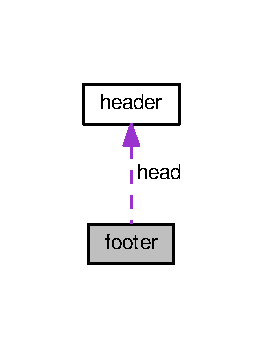
\includegraphics[width=128pt]{structfooter__coll__graph}
\end{center}
\end{figure}
\subsection*{Data Fields}
\begin{DoxyCompactItemize}
\item 
\hyperlink{structheader}{header} \hyperlink{structfooter_acae33dac61c9505ff5b850f88d32dd0b}{head}
\end{DoxyCompactItemize}


\subsection{Detailed Description}


Definition at line 16 of file heap.\+h.



\subsection{Field Documentation}
\index{footer@{footer}!head@{head}}
\index{head@{head}!footer@{footer}}
\subsubsection[{\texorpdfstring{head}{head}}]{\setlength{\rightskip}{0pt plus 5cm}{\bf header} footer\+::head}\hypertarget{structfooter_acae33dac61c9505ff5b850f88d32dd0b}{}\label{structfooter_acae33dac61c9505ff5b850f88d32dd0b}


Definition at line 17 of file heap.\+h.



The documentation for this struct was generated from the following file\+:\begin{DoxyCompactItemize}
\item 
/home/loudish/mpx-\/spring2017-\/modestus/mpx\+\_\+core/include/mem/\hyperlink{heap_8h}{heap.\+h}\end{DoxyCompactItemize}

\hypertarget{structgdt__descriptor__struct}{}\section{gdt\+\_\+descriptor\+\_\+struct Struct Reference}
\label{structgdt__descriptor__struct}\index{gdt\+\_\+descriptor\+\_\+struct@{gdt\+\_\+descriptor\+\_\+struct}}


{\ttfamily \#include $<$tables.\+h$>$}

\subsection*{Data Fields}
\begin{DoxyCompactItemize}
\item 
\hyperlink{system_8h_a863d9497073aad2b991aeab2211d87af}{u16int} \hyperlink{structgdt__descriptor__struct_a3c8ae013805dd982b25f0d62e3cdee0e}{limit}
\item 
\hyperlink{system_8h_a757de76cafbcddaac0d1632902fe4cb8}{u32int} \hyperlink{structgdt__descriptor__struct_aa47407e7b435c214d0cdd22cb66f0e71}{base}
\end{DoxyCompactItemize}


\subsection{Detailed Description}


Definition at line 23 of file tables.\+h.



\subsection{Field Documentation}
\index{gdt\+\_\+descriptor\+\_\+struct@{gdt\+\_\+descriptor\+\_\+struct}!base@{base}}
\index{base@{base}!gdt\+\_\+descriptor\+\_\+struct@{gdt\+\_\+descriptor\+\_\+struct}}
\subsubsection[{\texorpdfstring{base}{base}}]{\setlength{\rightskip}{0pt plus 5cm}{\bf u32int} gdt\+\_\+descriptor\+\_\+struct\+::base}\hypertarget{structgdt__descriptor__struct_aa47407e7b435c214d0cdd22cb66f0e71}{}\label{structgdt__descriptor__struct_aa47407e7b435c214d0cdd22cb66f0e71}


Definition at line 26 of file tables.\+h.

\index{gdt\+\_\+descriptor\+\_\+struct@{gdt\+\_\+descriptor\+\_\+struct}!limit@{limit}}
\index{limit@{limit}!gdt\+\_\+descriptor\+\_\+struct@{gdt\+\_\+descriptor\+\_\+struct}}
\subsubsection[{\texorpdfstring{limit}{limit}}]{\setlength{\rightskip}{0pt plus 5cm}{\bf u16int} gdt\+\_\+descriptor\+\_\+struct\+::limit}\hypertarget{structgdt__descriptor__struct_a3c8ae013805dd982b25f0d62e3cdee0e}{}\label{structgdt__descriptor__struct_a3c8ae013805dd982b25f0d62e3cdee0e}


Definition at line 25 of file tables.\+h.



The documentation for this struct was generated from the following file\+:\begin{DoxyCompactItemize}
\item 
/home/loudish/mpx-\/spring2017-\/modestus/mpx\+\_\+core/include/core/\hyperlink{tables_8h}{tables.\+h}\end{DoxyCompactItemize}

\hypertarget{structgdt__entry__struct}{}\section{gdt\+\_\+entry\+\_\+struct Struct Reference}
\label{structgdt__entry__struct}\index{gdt\+\_\+entry\+\_\+struct@{gdt\+\_\+entry\+\_\+struct}}


{\ttfamily \#include $<$tables.\+h$>$}

\subsection*{Data Fields}
\begin{DoxyCompactItemize}
\item 
\hyperlink{system_8h_a863d9497073aad2b991aeab2211d87af}{u16int} \hyperlink{structgdt__entry__struct_ada721fbdc3e8d3feae3b07d4b82a37bd}{limit\+\_\+low}
\item 
\hyperlink{system_8h_a863d9497073aad2b991aeab2211d87af}{u16int} \hyperlink{structgdt__entry__struct_a90f05cd7f227a34e977a639843a23275}{base\+\_\+low}
\item 
\hyperlink{system_8h_a1026e682ffdadc1701c42cd44ce9efcf}{u8int} \hyperlink{structgdt__entry__struct_a0369f1e190c433425c5b0f40c2070715}{base\+\_\+mid}
\item 
\hyperlink{system_8h_a1026e682ffdadc1701c42cd44ce9efcf}{u8int} \hyperlink{structgdt__entry__struct_a7457cb21f29e919a8ea62fc0110ac238}{access}
\item 
\hyperlink{system_8h_a1026e682ffdadc1701c42cd44ce9efcf}{u8int} \hyperlink{structgdt__entry__struct_afac75bdf53080168c8899c442862410a}{flags}
\item 
\hyperlink{system_8h_a1026e682ffdadc1701c42cd44ce9efcf}{u8int} \hyperlink{structgdt__entry__struct_aa03c14867c293012449a3b18a07f45f2}{base\+\_\+high}
\end{DoxyCompactItemize}


\subsection{Detailed Description}


Definition at line 30 of file tables.\+h.



\subsection{Field Documentation}
\index{gdt\+\_\+entry\+\_\+struct@{gdt\+\_\+entry\+\_\+struct}!access@{access}}
\index{access@{access}!gdt\+\_\+entry\+\_\+struct@{gdt\+\_\+entry\+\_\+struct}}
\subsubsection[{\texorpdfstring{access}{access}}]{\setlength{\rightskip}{0pt plus 5cm}{\bf u8int} gdt\+\_\+entry\+\_\+struct\+::access}\hypertarget{structgdt__entry__struct_a7457cb21f29e919a8ea62fc0110ac238}{}\label{structgdt__entry__struct_a7457cb21f29e919a8ea62fc0110ac238}


Definition at line 35 of file tables.\+h.

\index{gdt\+\_\+entry\+\_\+struct@{gdt\+\_\+entry\+\_\+struct}!base\+\_\+high@{base\+\_\+high}}
\index{base\+\_\+high@{base\+\_\+high}!gdt\+\_\+entry\+\_\+struct@{gdt\+\_\+entry\+\_\+struct}}
\subsubsection[{\texorpdfstring{base\+\_\+high}{base_high}}]{\setlength{\rightskip}{0pt plus 5cm}{\bf u8int} gdt\+\_\+entry\+\_\+struct\+::base\+\_\+high}\hypertarget{structgdt__entry__struct_aa03c14867c293012449a3b18a07f45f2}{}\label{structgdt__entry__struct_aa03c14867c293012449a3b18a07f45f2}


Definition at line 37 of file tables.\+h.

\index{gdt\+\_\+entry\+\_\+struct@{gdt\+\_\+entry\+\_\+struct}!base\+\_\+low@{base\+\_\+low}}
\index{base\+\_\+low@{base\+\_\+low}!gdt\+\_\+entry\+\_\+struct@{gdt\+\_\+entry\+\_\+struct}}
\subsubsection[{\texorpdfstring{base\+\_\+low}{base_low}}]{\setlength{\rightskip}{0pt plus 5cm}{\bf u16int} gdt\+\_\+entry\+\_\+struct\+::base\+\_\+low}\hypertarget{structgdt__entry__struct_a90f05cd7f227a34e977a639843a23275}{}\label{structgdt__entry__struct_a90f05cd7f227a34e977a639843a23275}


Definition at line 33 of file tables.\+h.

\index{gdt\+\_\+entry\+\_\+struct@{gdt\+\_\+entry\+\_\+struct}!base\+\_\+mid@{base\+\_\+mid}}
\index{base\+\_\+mid@{base\+\_\+mid}!gdt\+\_\+entry\+\_\+struct@{gdt\+\_\+entry\+\_\+struct}}
\subsubsection[{\texorpdfstring{base\+\_\+mid}{base_mid}}]{\setlength{\rightskip}{0pt plus 5cm}{\bf u8int} gdt\+\_\+entry\+\_\+struct\+::base\+\_\+mid}\hypertarget{structgdt__entry__struct_a0369f1e190c433425c5b0f40c2070715}{}\label{structgdt__entry__struct_a0369f1e190c433425c5b0f40c2070715}


Definition at line 34 of file tables.\+h.

\index{gdt\+\_\+entry\+\_\+struct@{gdt\+\_\+entry\+\_\+struct}!flags@{flags}}
\index{flags@{flags}!gdt\+\_\+entry\+\_\+struct@{gdt\+\_\+entry\+\_\+struct}}
\subsubsection[{\texorpdfstring{flags}{flags}}]{\setlength{\rightskip}{0pt plus 5cm}{\bf u8int} gdt\+\_\+entry\+\_\+struct\+::flags}\hypertarget{structgdt__entry__struct_afac75bdf53080168c8899c442862410a}{}\label{structgdt__entry__struct_afac75bdf53080168c8899c442862410a}


Definition at line 36 of file tables.\+h.

\index{gdt\+\_\+entry\+\_\+struct@{gdt\+\_\+entry\+\_\+struct}!limit\+\_\+low@{limit\+\_\+low}}
\index{limit\+\_\+low@{limit\+\_\+low}!gdt\+\_\+entry\+\_\+struct@{gdt\+\_\+entry\+\_\+struct}}
\subsubsection[{\texorpdfstring{limit\+\_\+low}{limit_low}}]{\setlength{\rightskip}{0pt plus 5cm}{\bf u16int} gdt\+\_\+entry\+\_\+struct\+::limit\+\_\+low}\hypertarget{structgdt__entry__struct_ada721fbdc3e8d3feae3b07d4b82a37bd}{}\label{structgdt__entry__struct_ada721fbdc3e8d3feae3b07d4b82a37bd}


Definition at line 32 of file tables.\+h.



The documentation for this struct was generated from the following file\+:\begin{DoxyCompactItemize}
\item 
/home/loudish/mpx-\/spring2017-\/modestus/mpx\+\_\+core/include/core/\hyperlink{tables_8h}{tables.\+h}\end{DoxyCompactItemize}

\hypertarget{structheader}{}\section{header Struct Reference}
\label{structheader}\index{header@{header}}


{\ttfamily \#include $<$heap.\+h$>$}

\subsection*{Data Fields}
\begin{DoxyCompactItemize}
\item 
int \hyperlink{structheader_af8cc659f702446226bc2ebabba437d5d}{size}
\item 
int \hyperlink{structheader_aec42bcd6139d12f84d54b5e6a149b276}{index\+\_\+id}
\end{DoxyCompactItemize}


\subsection{Detailed Description}


Definition at line 11 of file heap.\+h.



\subsection{Field Documentation}
\index{header@{header}!index\+\_\+id@{index\+\_\+id}}
\index{index\+\_\+id@{index\+\_\+id}!header@{header}}
\subsubsection[{\texorpdfstring{index\+\_\+id}{index_id}}]{\setlength{\rightskip}{0pt plus 5cm}int header\+::index\+\_\+id}\hypertarget{structheader_aec42bcd6139d12f84d54b5e6a149b276}{}\label{structheader_aec42bcd6139d12f84d54b5e6a149b276}


Definition at line 13 of file heap.\+h.

\index{header@{header}!size@{size}}
\index{size@{size}!header@{header}}
\subsubsection[{\texorpdfstring{size}{size}}]{\setlength{\rightskip}{0pt plus 5cm}int header\+::size}\hypertarget{structheader_af8cc659f702446226bc2ebabba437d5d}{}\label{structheader_af8cc659f702446226bc2ebabba437d5d}


Definition at line 12 of file heap.\+h.



The documentation for this struct was generated from the following file\+:\begin{DoxyCompactItemize}
\item 
/home/loudish/mpx-\/spring2017-\/modestus/mpx\+\_\+core/include/mem/\hyperlink{heap_8h}{heap.\+h}\end{DoxyCompactItemize}

\hypertarget{structheap}{}\section{heap Struct Reference}
\label{structheap}\index{heap@{heap}}


{\ttfamily \#include $<$heap.\+h$>$}



Collaboration diagram for heap\+:\nopagebreak
\begin{figure}[H]
\begin{center}
\leavevmode
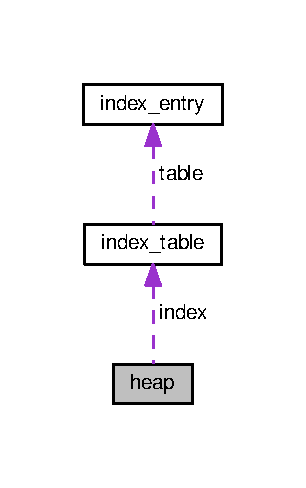
\includegraphics[width=147pt]{structheap__coll__graph}
\end{center}
\end{figure}
\subsection*{Data Fields}
\begin{DoxyCompactItemize}
\item 
\hyperlink{structindex__table}{index\+\_\+table} \hyperlink{structheap_a8fe6ce2a8b45088990071e9b1d35add2}{index}
\item 
\hyperlink{system_8h_a757de76cafbcddaac0d1632902fe4cb8}{u32int} \hyperlink{structheap_a744634662f1ffdb4d85632e68c063e51}{base}
\item 
\hyperlink{system_8h_a757de76cafbcddaac0d1632902fe4cb8}{u32int} \hyperlink{structheap_ad2e0262828735d6e437facbfce37d6b0}{max\+\_\+size}
\item 
\hyperlink{system_8h_a757de76cafbcddaac0d1632902fe4cb8}{u32int} \hyperlink{structheap_a7b4422774c5ca7ac8ed5ddfe95f5c8ec}{min\+\_\+size}
\end{DoxyCompactItemize}


\subsection{Detailed Description}


Definition at line 33 of file heap.\+h.



\subsection{Field Documentation}
\index{heap@{heap}!base@{base}}
\index{base@{base}!heap@{heap}}
\subsubsection[{\texorpdfstring{base}{base}}]{\setlength{\rightskip}{0pt plus 5cm}{\bf u32int} heap\+::base}\hypertarget{structheap_a744634662f1ffdb4d85632e68c063e51}{}\label{structheap_a744634662f1ffdb4d85632e68c063e51}


Definition at line 35 of file heap.\+h.

\index{heap@{heap}!index@{index}}
\index{index@{index}!heap@{heap}}
\subsubsection[{\texorpdfstring{index}{index}}]{\setlength{\rightskip}{0pt plus 5cm}{\bf index\+\_\+table} heap\+::index}\hypertarget{structheap_a8fe6ce2a8b45088990071e9b1d35add2}{}\label{structheap_a8fe6ce2a8b45088990071e9b1d35add2}


Definition at line 34 of file heap.\+h.

\index{heap@{heap}!max\+\_\+size@{max\+\_\+size}}
\index{max\+\_\+size@{max\+\_\+size}!heap@{heap}}
\subsubsection[{\texorpdfstring{max\+\_\+size}{max_size}}]{\setlength{\rightskip}{0pt plus 5cm}{\bf u32int} heap\+::max\+\_\+size}\hypertarget{structheap_ad2e0262828735d6e437facbfce37d6b0}{}\label{structheap_ad2e0262828735d6e437facbfce37d6b0}


Definition at line 36 of file heap.\+h.

\index{heap@{heap}!min\+\_\+size@{min\+\_\+size}}
\index{min\+\_\+size@{min\+\_\+size}!heap@{heap}}
\subsubsection[{\texorpdfstring{min\+\_\+size}{min_size}}]{\setlength{\rightskip}{0pt plus 5cm}{\bf u32int} heap\+::min\+\_\+size}\hypertarget{structheap_a7b4422774c5ca7ac8ed5ddfe95f5c8ec}{}\label{structheap_a7b4422774c5ca7ac8ed5ddfe95f5c8ec}


Definition at line 37 of file heap.\+h.



The documentation for this struct was generated from the following file\+:\begin{DoxyCompactItemize}
\item 
/home/loudish/mpx-\/spring2017-\/modestus/mpx\+\_\+core/include/mem/\hyperlink{heap_8h}{heap.\+h}\end{DoxyCompactItemize}

\hypertarget{structidt__entry__struct}{}\section{idt\+\_\+entry\+\_\+struct Struct Reference}
\label{structidt__entry__struct}\index{idt\+\_\+entry\+\_\+struct@{idt\+\_\+entry\+\_\+struct}}


{\ttfamily \#include $<$tables.\+h$>$}

\subsection*{Data Fields}
\begin{DoxyCompactItemize}
\item 
\hyperlink{system_8h_a863d9497073aad2b991aeab2211d87af}{u16int} \hyperlink{structidt__entry__struct_aefa75d6bfe07f1f544393b4dbccb3e76}{base\+\_\+low}
\item 
\hyperlink{system_8h_a863d9497073aad2b991aeab2211d87af}{u16int} \hyperlink{structidt__entry__struct_a85254c7df6a612f4a4b3bb470ff3370c}{sselect}
\item 
\hyperlink{system_8h_a1026e682ffdadc1701c42cd44ce9efcf}{u8int} \hyperlink{structidt__entry__struct_a0d33c8509ae77d42e680d8d11b4c8035}{zero}
\item 
\hyperlink{system_8h_a1026e682ffdadc1701c42cd44ce9efcf}{u8int} \hyperlink{structidt__entry__struct_a46c92bd8f07d5ff4e379a07b293c46af}{flags}
\item 
\hyperlink{system_8h_a863d9497073aad2b991aeab2211d87af}{u16int} \hyperlink{structidt__entry__struct_a1c6a29cae5ea9a832cf4261aaa5b43d0}{base\+\_\+high}
\end{DoxyCompactItemize}


\subsection{Detailed Description}


Definition at line 6 of file tables.\+h.



\subsection{Field Documentation}
\index{idt\+\_\+entry\+\_\+struct@{idt\+\_\+entry\+\_\+struct}!base\+\_\+high@{base\+\_\+high}}
\index{base\+\_\+high@{base\+\_\+high}!idt\+\_\+entry\+\_\+struct@{idt\+\_\+entry\+\_\+struct}}
\subsubsection[{\texorpdfstring{base\+\_\+high}{base_high}}]{\setlength{\rightskip}{0pt plus 5cm}{\bf u16int} idt\+\_\+entry\+\_\+struct\+::base\+\_\+high}\hypertarget{structidt__entry__struct_a1c6a29cae5ea9a832cf4261aaa5b43d0}{}\label{structidt__entry__struct_a1c6a29cae5ea9a832cf4261aaa5b43d0}


Definition at line 12 of file tables.\+h.

\index{idt\+\_\+entry\+\_\+struct@{idt\+\_\+entry\+\_\+struct}!base\+\_\+low@{base\+\_\+low}}
\index{base\+\_\+low@{base\+\_\+low}!idt\+\_\+entry\+\_\+struct@{idt\+\_\+entry\+\_\+struct}}
\subsubsection[{\texorpdfstring{base\+\_\+low}{base_low}}]{\setlength{\rightskip}{0pt plus 5cm}{\bf u16int} idt\+\_\+entry\+\_\+struct\+::base\+\_\+low}\hypertarget{structidt__entry__struct_aefa75d6bfe07f1f544393b4dbccb3e76}{}\label{structidt__entry__struct_aefa75d6bfe07f1f544393b4dbccb3e76}


Definition at line 8 of file tables.\+h.

\index{idt\+\_\+entry\+\_\+struct@{idt\+\_\+entry\+\_\+struct}!flags@{flags}}
\index{flags@{flags}!idt\+\_\+entry\+\_\+struct@{idt\+\_\+entry\+\_\+struct}}
\subsubsection[{\texorpdfstring{flags}{flags}}]{\setlength{\rightskip}{0pt plus 5cm}{\bf u8int} idt\+\_\+entry\+\_\+struct\+::flags}\hypertarget{structidt__entry__struct_a46c92bd8f07d5ff4e379a07b293c46af}{}\label{structidt__entry__struct_a46c92bd8f07d5ff4e379a07b293c46af}


Definition at line 11 of file tables.\+h.

\index{idt\+\_\+entry\+\_\+struct@{idt\+\_\+entry\+\_\+struct}!sselect@{sselect}}
\index{sselect@{sselect}!idt\+\_\+entry\+\_\+struct@{idt\+\_\+entry\+\_\+struct}}
\subsubsection[{\texorpdfstring{sselect}{sselect}}]{\setlength{\rightskip}{0pt plus 5cm}{\bf u16int} idt\+\_\+entry\+\_\+struct\+::sselect}\hypertarget{structidt__entry__struct_a85254c7df6a612f4a4b3bb470ff3370c}{}\label{structidt__entry__struct_a85254c7df6a612f4a4b3bb470ff3370c}


Definition at line 9 of file tables.\+h.

\index{idt\+\_\+entry\+\_\+struct@{idt\+\_\+entry\+\_\+struct}!zero@{zero}}
\index{zero@{zero}!idt\+\_\+entry\+\_\+struct@{idt\+\_\+entry\+\_\+struct}}
\subsubsection[{\texorpdfstring{zero}{zero}}]{\setlength{\rightskip}{0pt plus 5cm}{\bf u8int} idt\+\_\+entry\+\_\+struct\+::zero}\hypertarget{structidt__entry__struct_a0d33c8509ae77d42e680d8d11b4c8035}{}\label{structidt__entry__struct_a0d33c8509ae77d42e680d8d11b4c8035}


Definition at line 10 of file tables.\+h.



The documentation for this struct was generated from the following file\+:\begin{DoxyCompactItemize}
\item 
/home/loudish/mpx-\/spring2017-\/modestus/mpx\+\_\+core/include/core/\hyperlink{tables_8h}{tables.\+h}\end{DoxyCompactItemize}

\hypertarget{structidt__struct}{}\section{idt\+\_\+struct Struct Reference}
\label{structidt__struct}\index{idt\+\_\+struct@{idt\+\_\+struct}}


{\ttfamily \#include $<$tables.\+h$>$}

\subsection*{Data Fields}
\begin{DoxyCompactItemize}
\item 
\hyperlink{system_8h_a863d9497073aad2b991aeab2211d87af}{u16int} \hyperlink{structidt__struct_aa75e2805e21db1a33816af778263d712}{limit}
\item 
\hyperlink{system_8h_a757de76cafbcddaac0d1632902fe4cb8}{u32int} \hyperlink{structidt__struct_a1a91fe2ab44ad8dfbad0f6d07ec789ea}{base}
\end{DoxyCompactItemize}


\subsection{Detailed Description}


Definition at line 16 of file tables.\+h.



\subsection{Field Documentation}
\index{idt\+\_\+struct@{idt\+\_\+struct}!base@{base}}
\index{base@{base}!idt\+\_\+struct@{idt\+\_\+struct}}
\subsubsection[{\texorpdfstring{base}{base}}]{\setlength{\rightskip}{0pt plus 5cm}{\bf u32int} idt\+\_\+struct\+::base}\hypertarget{structidt__struct_a1a91fe2ab44ad8dfbad0f6d07ec789ea}{}\label{structidt__struct_a1a91fe2ab44ad8dfbad0f6d07ec789ea}


Definition at line 19 of file tables.\+h.

\index{idt\+\_\+struct@{idt\+\_\+struct}!limit@{limit}}
\index{limit@{limit}!idt\+\_\+struct@{idt\+\_\+struct}}
\subsubsection[{\texorpdfstring{limit}{limit}}]{\setlength{\rightskip}{0pt plus 5cm}{\bf u16int} idt\+\_\+struct\+::limit}\hypertarget{structidt__struct_aa75e2805e21db1a33816af778263d712}{}\label{structidt__struct_aa75e2805e21db1a33816af778263d712}


Definition at line 18 of file tables.\+h.



The documentation for this struct was generated from the following file\+:\begin{DoxyCompactItemize}
\item 
/home/loudish/mpx-\/spring2017-\/modestus/mpx\+\_\+core/include/core/\hyperlink{tables_8h}{tables.\+h}\end{DoxyCompactItemize}

\hypertarget{structindex__entry}{}\section{index\+\_\+entry Struct Reference}
\label{structindex__entry}\index{index\+\_\+entry@{index\+\_\+entry}}


{\ttfamily \#include $<$heap.\+h$>$}

\subsection*{Data Fields}
\begin{DoxyCompactItemize}
\item 
int \hyperlink{structindex__entry_a2b0247aae5c7f9884f8eef1ee121adb0}{size}
\item 
int \hyperlink{structindex__entry_afdbdffb4bd17e4ab003b94be3d5bade7}{empty}
\item 
\hyperlink{system_8h_a757de76cafbcddaac0d1632902fe4cb8}{u32int} \hyperlink{structindex__entry_a0a8d4dc0595b5f2ef42e7080c5221c1f}{block}
\end{DoxyCompactItemize}


\subsection{Detailed Description}


Definition at line 20 of file heap.\+h.



\subsection{Field Documentation}
\index{index\+\_\+entry@{index\+\_\+entry}!block@{block}}
\index{block@{block}!index\+\_\+entry@{index\+\_\+entry}}
\subsubsection[{\texorpdfstring{block}{block}}]{\setlength{\rightskip}{0pt plus 5cm}{\bf u32int} index\+\_\+entry\+::block}\hypertarget{structindex__entry_a0a8d4dc0595b5f2ef42e7080c5221c1f}{}\label{structindex__entry_a0a8d4dc0595b5f2ef42e7080c5221c1f}


Definition at line 23 of file heap.\+h.

\index{index\+\_\+entry@{index\+\_\+entry}!empty@{empty}}
\index{empty@{empty}!index\+\_\+entry@{index\+\_\+entry}}
\subsubsection[{\texorpdfstring{empty}{empty}}]{\setlength{\rightskip}{0pt plus 5cm}int index\+\_\+entry\+::empty}\hypertarget{structindex__entry_afdbdffb4bd17e4ab003b94be3d5bade7}{}\label{structindex__entry_afdbdffb4bd17e4ab003b94be3d5bade7}


Definition at line 22 of file heap.\+h.

\index{index\+\_\+entry@{index\+\_\+entry}!size@{size}}
\index{size@{size}!index\+\_\+entry@{index\+\_\+entry}}
\subsubsection[{\texorpdfstring{size}{size}}]{\setlength{\rightskip}{0pt plus 5cm}int index\+\_\+entry\+::size}\hypertarget{structindex__entry_a2b0247aae5c7f9884f8eef1ee121adb0}{}\label{structindex__entry_a2b0247aae5c7f9884f8eef1ee121adb0}


Definition at line 21 of file heap.\+h.



The documentation for this struct was generated from the following file\+:\begin{DoxyCompactItemize}
\item 
/home/loudish/mpx-\/spring2017-\/modestus/mpx\+\_\+core/include/mem/\hyperlink{heap_8h}{heap.\+h}\end{DoxyCompactItemize}

\hypertarget{structindex__table}{}\section{index\+\_\+table Struct Reference}
\label{structindex__table}\index{index\+\_\+table@{index\+\_\+table}}


{\ttfamily \#include $<$heap.\+h$>$}



Collaboration diagram for index\+\_\+table\+:\nopagebreak
\begin{figure}[H]
\begin{center}
\leavevmode
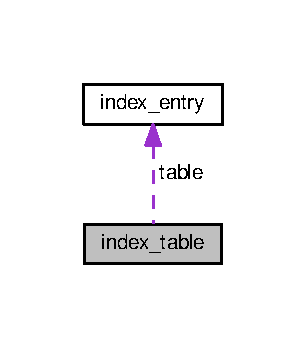
\includegraphics[width=147pt]{structindex__table__coll__graph}
\end{center}
\end{figure}
\subsection*{Data Fields}
\begin{DoxyCompactItemize}
\item 
\hyperlink{structindex__entry}{index\+\_\+entry} \hyperlink{structindex__table_ae69e0312bad59289ac303989d06c565d}{table} \mbox{[}\hyperlink{heap_8h_a032503e76d6f69bc67e99e909c8125da}{T\+A\+B\+L\+E\+\_\+\+S\+I\+ZE}\mbox{]}
\item 
int \hyperlink{structindex__table_a6e0e8e27a6a47e8ae2078b6fa447087f}{id}
\end{DoxyCompactItemize}


\subsection{Detailed Description}


Definition at line 27 of file heap.\+h.



\subsection{Field Documentation}
\index{index\+\_\+table@{index\+\_\+table}!id@{id}}
\index{id@{id}!index\+\_\+table@{index\+\_\+table}}
\subsubsection[{\texorpdfstring{id}{id}}]{\setlength{\rightskip}{0pt plus 5cm}int index\+\_\+table\+::id}\hypertarget{structindex__table_a6e0e8e27a6a47e8ae2078b6fa447087f}{}\label{structindex__table_a6e0e8e27a6a47e8ae2078b6fa447087f}


Definition at line 29 of file heap.\+h.

\index{index\+\_\+table@{index\+\_\+table}!table@{table}}
\index{table@{table}!index\+\_\+table@{index\+\_\+table}}
\subsubsection[{\texorpdfstring{table}{table}}]{\setlength{\rightskip}{0pt plus 5cm}{\bf index\+\_\+entry} index\+\_\+table\+::table\mbox{[}{\bf T\+A\+B\+L\+E\+\_\+\+S\+I\+ZE}\mbox{]}}\hypertarget{structindex__table_ae69e0312bad59289ac303989d06c565d}{}\label{structindex__table_ae69e0312bad59289ac303989d06c565d}


Definition at line 28 of file heap.\+h.



The documentation for this struct was generated from the following file\+:\begin{DoxyCompactItemize}
\item 
/home/loudish/mpx-\/spring2017-\/modestus/mpx\+\_\+core/include/mem/\hyperlink{heap_8h}{heap.\+h}\end{DoxyCompactItemize}

\hypertarget{structlinked_list__t}{}\section{linked\+List\+\_\+t Struct Reference}
\label{structlinked_list__t}\index{linked\+List\+\_\+t@{linked\+List\+\_\+t}}


typedef of linked list (see \hyperlink{structs__ll}{s\+\_\+ll}).  




{\ttfamily \#include $<$linked\+\_\+list$>$}



\subsection{Detailed Description}
typedef of linked list (see \hyperlink{structs__ll}{s\+\_\+ll}). 

\begin{DoxySeeAlso}{See also}
\hyperlink{structs__ll}{s\+\_\+ll} 

\hyperlink{linked__list_8h}{linked\+\_\+list.\+h} 
\end{DoxySeeAlso}


The documentation for this struct was generated from the following file\+:\begin{DoxyCompactItemize}
\item 
/home/loudish/mpx-\/spring2017-\/modestus/mpx\+\_\+core/include/\hyperlink{linked__list_8h}{linked\+\_\+list.\+h}\end{DoxyCompactItemize}

\hypertarget{structs__ll}{}\section{linked\+List\+\_\+t Struct Reference}
\label{structs__ll}\index{linked\+List\+\_\+t@{linked\+List\+\_\+t}}


struct definition for the linked list  




{\ttfamily \#include $<$linked\+\_\+list$>$}



Collaboration diagram for linked\+List\+\_\+t\+:\nopagebreak
\begin{figure}[H]
\begin{center}
\leavevmode
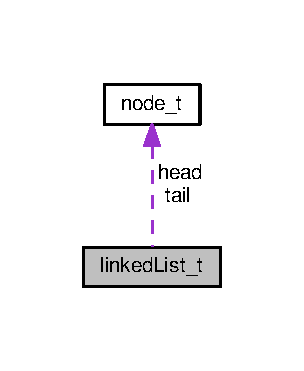
\includegraphics[width=146pt]{structs__ll__coll__graph}
\end{center}
\end{figure}
\subsection*{Data Fields}
\begin{DoxyCompactItemize}
\item 
\hyperlink{structnode__t}{node\+\_\+t} \hyperlink{structs__ll_a0056de8ffd1d9af11ed1a8bb771ae227}{head}
\item 
\hyperlink{structnode__t}{node\+\_\+t} \hyperlink{structs__ll_a3253fe5f72d8914dd8331e74aba9982e}{tail}
\item 
int($\ast$ \hyperlink{structs__ll_ac22c97ea79a7ec45eb27584f2f91295c}{search\+Comp\+Func} )(void $\ast$, void $\ast$)
\item 
int($\ast$ \hyperlink{structs__ll_accf6a1a7fe14f0693107a00a47b86d0d}{insert\+Comp\+Func} )(void $\ast$, void $\ast$)
\item 
int($\ast$ \hyperlink{structs__ll_a3cf5521a73fc3474e83aef51c777bb7f}{free\+Node\+Func} )(\hyperlink{structnode__t}{node\+\_\+t} $\ast$node\+To\+Free)
\item 
void($\ast$ \hyperlink{structs__ll_ad3b310fea19fca7898583a8c0eb87449}{print\+Node\+Func} )(void $\ast$)
\item 
\hyperlink{system_8h_a7c94ea6f8948649f8d181ae55911eeaf}{size\+\_\+t} \hyperlink{structs__ll_abeb40a7e7b4c71ba09151cde4005c201}{length}
\end{DoxyCompactItemize}


\subsection{Detailed Description}
struct definition for the linked list 

\begin{DoxySeeAlso}{See also}
\hyperlink{linked__list_8h}{linked\+\_\+list.\+h} 
\end{DoxySeeAlso}


Definition at line 62 of file linked\+\_\+list.\+h.



\subsection{Field Documentation}
\index{s\+\_\+ll@{s\+\_\+ll}!free\+Node\+Func@{free\+Node\+Func}}
\index{free\+Node\+Func@{free\+Node\+Func}!s\+\_\+ll@{s\+\_\+ll}}
\subsubsection[{\texorpdfstring{free\+Node\+Func}{freeNodeFunc}}]{\setlength{\rightskip}{0pt plus 5cm}int($\ast$ linked\+List\+\_\+t\+::free\+Node\+Func) ({\bf node\+\_\+t} $\ast$node\+To\+Free)}\hypertarget{structs__ll_a3cf5521a73fc3474e83aef51c777bb7f}{}\label{structs__ll_a3cf5521a73fc3474e83aef51c777bb7f}
\begin{DoxySeeAlso}{See also}
\hyperlink{linked__list_8c_a45d030386936adffa3eb5586ce93d131}{set\+Insert\+Comparison\+Function} 
\end{DoxySeeAlso}


Definition at line 68 of file linked\+\_\+list.\+h.

\index{s\+\_\+ll@{s\+\_\+ll}!head@{head}}
\index{head@{head}!s\+\_\+ll@{s\+\_\+ll}}
\subsubsection[{\texorpdfstring{head}{head}}]{\setlength{\rightskip}{0pt plus 5cm}{\bf node\+\_\+t} linked\+List\+\_\+t\+::head}\hypertarget{structs__ll_a0056de8ffd1d9af11ed1a8bb771ae227}{}\label{structs__ll_a0056de8ffd1d9af11ed1a8bb771ae227}


Definition at line 64 of file linked\+\_\+list.\+h.

\index{s\+\_\+ll@{s\+\_\+ll}!insert\+Comp\+Func@{insert\+Comp\+Func}}
\index{insert\+Comp\+Func@{insert\+Comp\+Func}!s\+\_\+ll@{s\+\_\+ll}}
\subsubsection[{\texorpdfstring{insert\+Comp\+Func}{insertCompFunc}}]{\setlength{\rightskip}{0pt plus 5cm}int($\ast$ linked\+List\+\_\+t\+::insert\+Comp\+Func) (void $\ast$, void $\ast$)}\hypertarget{structs__ll_accf6a1a7fe14f0693107a00a47b86d0d}{}\label{structs__ll_accf6a1a7fe14f0693107a00a47b86d0d}
\begin{DoxySeeAlso}{See also}
\hyperlink{linked__list_8c_a12e5138ac02af0f6b42ff2f1b29c610a}{set\+Search\+Comparison\+Function} 
\end{DoxySeeAlso}


Definition at line 67 of file linked\+\_\+list.\+h.

\index{s\+\_\+ll@{s\+\_\+ll}!length@{length}}
\index{length@{length}!s\+\_\+ll@{s\+\_\+ll}}
\subsubsection[{\texorpdfstring{length}{length}}]{\setlength{\rightskip}{0pt plus 5cm}{\bf size\+\_\+t} linked\+List\+\_\+t\+::length}\hypertarget{structs__ll_abeb40a7e7b4c71ba09151cde4005c201}{}\label{structs__ll_abeb40a7e7b4c71ba09151cde4005c201}
\begin{DoxySeeAlso}{See also}
\hyperlink{group___r2_gafc8969d7969f61c928a01f4c302e669b}{set\+Print\+Function} 
\end{DoxySeeAlso}


Definition at line 70 of file linked\+\_\+list.\+h.

\index{s\+\_\+ll@{s\+\_\+ll}!print\+Node\+Func@{print\+Node\+Func}}
\index{print\+Node\+Func@{print\+Node\+Func}!s\+\_\+ll@{s\+\_\+ll}}
\subsubsection[{\texorpdfstring{print\+Node\+Func}{printNodeFunc}}]{\setlength{\rightskip}{0pt plus 5cm}void($\ast$ linked\+List\+\_\+t\+::print\+Node\+Func) (void $\ast$)}\hypertarget{structs__ll_ad3b310fea19fca7898583a8c0eb87449}{}\label{structs__ll_ad3b310fea19fca7898583a8c0eb87449}
\begin{DoxySeeAlso}{See also}
\hyperlink{linked__list_8c_a3b6f817f74d12d2cf4a35405f447c73d}{set\+Free\+Function} 
\end{DoxySeeAlso}


Definition at line 69 of file linked\+\_\+list.\+h.

\index{s\+\_\+ll@{s\+\_\+ll}!search\+Comp\+Func@{search\+Comp\+Func}}
\index{search\+Comp\+Func@{search\+Comp\+Func}!s\+\_\+ll@{s\+\_\+ll}}
\subsubsection[{\texorpdfstring{search\+Comp\+Func}{searchCompFunc}}]{\setlength{\rightskip}{0pt plus 5cm}int($\ast$ linked\+List\+\_\+t\+::search\+Comp\+Func) (void $\ast$, void $\ast$)}\hypertarget{structs__ll_ac22c97ea79a7ec45eb27584f2f91295c}{}\label{structs__ll_ac22c97ea79a7ec45eb27584f2f91295c}


Definition at line 66 of file linked\+\_\+list.\+h.

\index{s\+\_\+ll@{s\+\_\+ll}!tail@{tail}}
\index{tail@{tail}!s\+\_\+ll@{s\+\_\+ll}}
\subsubsection[{\texorpdfstring{tail}{tail}}]{\setlength{\rightskip}{0pt plus 5cm}{\bf node\+\_\+t} linked\+List\+\_\+t\+::tail}\hypertarget{structs__ll_a3253fe5f72d8914dd8331e74aba9982e}{}\label{structs__ll_a3253fe5f72d8914dd8331e74aba9982e}


Definition at line 65 of file linked\+\_\+list.\+h.



The documentation for this struct was generated from the following file\+:\begin{DoxyCompactItemize}
\item 
/home/loudish/mpx-\/spring2017-\/modestus/mpx\+\_\+core/include/\hyperlink{linked__list_8h}{linked\+\_\+list.\+h}\end{DoxyCompactItemize}

\hypertarget{structnode__t}{}\section{node\+\_\+t Struct Reference}
\label{structnode__t}\index{node\+\_\+t@{node\+\_\+t}}


typedef of linked list node (see \hyperlink{structs__ll__node}{s\+\_\+ll\+\_\+node}).  




{\ttfamily \#include $<$linked\+\_\+list$>$}



\subsection{Detailed Description}
typedef of linked list node (see \hyperlink{structs__ll__node}{s\+\_\+ll\+\_\+node}). 

\begin{DoxySeeAlso}{See also}
\hyperlink{structs__ll__node}{s\+\_\+ll\+\_\+node} 

\hyperlink{linked__list_8h}{linked\+\_\+list.\+h} 
\end{DoxySeeAlso}


The documentation for this struct was generated from the following file\+:\begin{DoxyCompactItemize}
\item 
/home/loudish/mpx-\/spring2017-\/modestus/mpx\+\_\+core/include/\hyperlink{linked__list_8h}{linked\+\_\+list.\+h}\end{DoxyCompactItemize}

\hypertarget{structs__ll__node}{}\section{node\+\_\+t Struct Reference}
\label{structs__ll__node}\index{node\+\_\+t@{node\+\_\+t}}


struct for a node of the linked list  




{\ttfamily \#include $<$linked\+\_\+list$>$}



Collaboration diagram for node\+\_\+t\+:\nopagebreak
\begin{figure}[H]
\begin{center}
\leavevmode
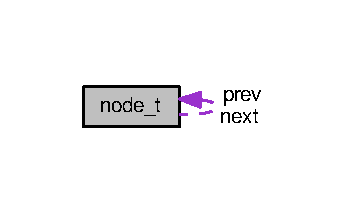
\includegraphics[width=166pt]{structs__ll__node__coll__graph}
\end{center}
\end{figure}
\subsection*{Data Fields}
\begin{DoxyCompactItemize}
\item 
void $\ast$ \hyperlink{structs__ll__node_aa69340d9d81a183ddfbfec74a7524966}{data}
\item 
\hyperlink{structnode__t}{node\+\_\+t} $\ast$ \hyperlink{structs__ll__node_a3eaaa938f4adef906b28c0afcaf511d6}{next}
\item 
\hyperlink{structnode__t}{node\+\_\+t} $\ast$ \hyperlink{structs__ll__node_a19e812d499f3cd75491d7ab5b1d08e6c}{prev}
\end{DoxyCompactItemize}


\subsection{Detailed Description}
struct for a node of the linked list 

\begin{DoxySeeAlso}{See also}
\hyperlink{structs__ll}{s\+\_\+ll} 

\hyperlink{linked__list_8h}{linked\+\_\+list.\+h} 
\end{DoxySeeAlso}


Definition at line 46 of file linked\+\_\+list.\+h.



\subsection{Field Documentation}
\index{s\+\_\+ll\+\_\+node@{s\+\_\+ll\+\_\+node}!data@{data}}
\index{data@{data}!s\+\_\+ll\+\_\+node@{s\+\_\+ll\+\_\+node}}
\subsubsection[{\texorpdfstring{data}{data}}]{\setlength{\rightskip}{0pt plus 5cm}void$\ast$ node\+\_\+t\+::data}\hypertarget{structs__ll__node_aa69340d9d81a183ddfbfec74a7524966}{}\label{structs__ll__node_aa69340d9d81a183ddfbfec74a7524966}


Definition at line 48 of file linked\+\_\+list.\+h.

\index{s\+\_\+ll\+\_\+node@{s\+\_\+ll\+\_\+node}!next@{next}}
\index{next@{next}!s\+\_\+ll\+\_\+node@{s\+\_\+ll\+\_\+node}}
\subsubsection[{\texorpdfstring{next}{next}}]{\setlength{\rightskip}{0pt plus 5cm}{\bf node\+\_\+t}$\ast$ node\+\_\+t\+::next}\hypertarget{structs__ll__node_a3eaaa938f4adef906b28c0afcaf511d6}{}\label{structs__ll__node_a3eaaa938f4adef906b28c0afcaf511d6}


Definition at line 49 of file linked\+\_\+list.\+h.

\index{s\+\_\+ll\+\_\+node@{s\+\_\+ll\+\_\+node}!prev@{prev}}
\index{prev@{prev}!s\+\_\+ll\+\_\+node@{s\+\_\+ll\+\_\+node}}
\subsubsection[{\texorpdfstring{prev}{prev}}]{\setlength{\rightskip}{0pt plus 5cm}{\bf node\+\_\+t}$\ast$ node\+\_\+t\+::prev}\hypertarget{structs__ll__node_a19e812d499f3cd75491d7ab5b1d08e6c}{}\label{structs__ll__node_a19e812d499f3cd75491d7ab5b1d08e6c}


Definition at line 50 of file linked\+\_\+list.\+h.



The documentation for this struct was generated from the following file\+:\begin{DoxyCompactItemize}
\item 
/home/loudish/mpx-\/spring2017-\/modestus/mpx\+\_\+core/include/\hyperlink{linked__list_8h}{linked\+\_\+list.\+h}\end{DoxyCompactItemize}

\hypertarget{structpage__dir}{}\section{page\+\_\+dir Struct Reference}
\label{structpage__dir}\index{page\+\_\+dir@{page\+\_\+dir}}


{\ttfamily \#include $<$paging.\+h$>$}



Collaboration diagram for page\+\_\+dir\+:\nopagebreak
\begin{figure}[H]
\begin{center}
\leavevmode
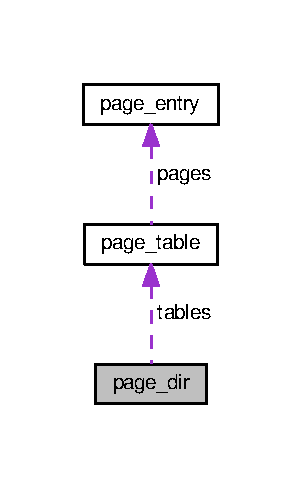
\includegraphics[width=145pt]{structpage__dir__coll__graph}
\end{center}
\end{figure}
\subsection*{Data Fields}
\begin{DoxyCompactItemize}
\item 
\hyperlink{structpage__table}{page\+\_\+table} $\ast$ \hyperlink{structpage__dir_ac89434e3fccabfe9481ea77fdda82faf}{tables} \mbox{[}1024\mbox{]}
\item 
\hyperlink{system_8h_a757de76cafbcddaac0d1632902fe4cb8}{u32int} \hyperlink{structpage__dir_a7336b695acaf516613dda626129129d0}{tables\+\_\+phys} \mbox{[}1024\mbox{]}
\end{DoxyCompactItemize}


\subsection{Detailed Description}


Definition at line 34 of file paging.\+h.



\subsection{Field Documentation}
\index{page\+\_\+dir@{page\+\_\+dir}!tables@{tables}}
\index{tables@{tables}!page\+\_\+dir@{page\+\_\+dir}}
\subsubsection[{\texorpdfstring{tables}{tables}}]{\setlength{\rightskip}{0pt plus 5cm}{\bf page\+\_\+table}$\ast$ page\+\_\+dir\+::tables\mbox{[}1024\mbox{]}}\hypertarget{structpage__dir_ac89434e3fccabfe9481ea77fdda82faf}{}\label{structpage__dir_ac89434e3fccabfe9481ea77fdda82faf}


Definition at line 35 of file paging.\+h.



Referenced by get\+\_\+page().

\index{page\+\_\+dir@{page\+\_\+dir}!tables\+\_\+phys@{tables\+\_\+phys}}
\index{tables\+\_\+phys@{tables\+\_\+phys}!page\+\_\+dir@{page\+\_\+dir}}
\subsubsection[{\texorpdfstring{tables\+\_\+phys}{tables_phys}}]{\setlength{\rightskip}{0pt plus 5cm}{\bf u32int} page\+\_\+dir\+::tables\+\_\+phys\mbox{[}1024\mbox{]}}\hypertarget{structpage__dir_a7336b695acaf516613dda626129129d0}{}\label{structpage__dir_a7336b695acaf516613dda626129129d0}


Definition at line 36 of file paging.\+h.



Referenced by get\+\_\+page(), and load\+\_\+page\+\_\+dir().



The documentation for this struct was generated from the following file\+:\begin{DoxyCompactItemize}
\item 
/home/loudish/mpx-\/spring2017-\/modestus/mpx\+\_\+core/include/mem/\hyperlink{paging_8h}{paging.\+h}\end{DoxyCompactItemize}

\hypertarget{structpage__entry}{}\section{page\+\_\+entry Struct Reference}
\label{structpage__entry}\index{page\+\_\+entry@{page\+\_\+entry}}


{\ttfamily \#include $<$paging.\+h$>$}

\subsection*{Data Fields}
\begin{DoxyCompactItemize}
\item 
\hyperlink{system_8h_a757de76cafbcddaac0d1632902fe4cb8}{u32int} \hyperlink{structpage__entry_a34148a94af9bfabbb8c4f00f9865dfee}{present}\+: 1
\item 
\hyperlink{system_8h_a757de76cafbcddaac0d1632902fe4cb8}{u32int} \hyperlink{structpage__entry_a2ea8d7684fe45772b6acba70d46e41d9}{writeable}\+: 1
\item 
\hyperlink{system_8h_a757de76cafbcddaac0d1632902fe4cb8}{u32int} \hyperlink{structpage__entry_a2beafd3900a1f36f09af9c35a9a14f18}{usermode}\+: 1
\item 
\hyperlink{system_8h_a757de76cafbcddaac0d1632902fe4cb8}{u32int} \hyperlink{structpage__entry_a8b4097e0cee08d028182b11bd1f73f92}{accessed}\+: 1
\item 
\hyperlink{system_8h_a757de76cafbcddaac0d1632902fe4cb8}{u32int} \hyperlink{structpage__entry_ab3b5e22c6146f227a26bdec64e63f4b0}{dirty}\+: 1
\item 
\hyperlink{system_8h_a757de76cafbcddaac0d1632902fe4cb8}{u32int} \hyperlink{structpage__entry_af6d963f09b01571b107e6f505050c0e5}{reserved}\+: 7
\item 
\hyperlink{system_8h_a757de76cafbcddaac0d1632902fe4cb8}{u32int} \hyperlink{structpage__entry_a68a6dc54a7ab6f7fb1a068476190bf67}{frameaddr}\+: 20
\end{DoxyCompactItemize}


\subsection{Detailed Description}


Definition at line 12 of file paging.\+h.



\subsection{Field Documentation}
\index{page\+\_\+entry@{page\+\_\+entry}!accessed@{accessed}}
\index{accessed@{accessed}!page\+\_\+entry@{page\+\_\+entry}}
\subsubsection[{\texorpdfstring{accessed}{accessed}}]{\setlength{\rightskip}{0pt plus 5cm}{\bf u32int} page\+\_\+entry\+::accessed}\hypertarget{structpage__entry_a8b4097e0cee08d028182b11bd1f73f92}{}\label{structpage__entry_a8b4097e0cee08d028182b11bd1f73f92}


Definition at line 16 of file paging.\+h.

\index{page\+\_\+entry@{page\+\_\+entry}!dirty@{dirty}}
\index{dirty@{dirty}!page\+\_\+entry@{page\+\_\+entry}}
\subsubsection[{\texorpdfstring{dirty}{dirty}}]{\setlength{\rightskip}{0pt plus 5cm}{\bf u32int} page\+\_\+entry\+::dirty}\hypertarget{structpage__entry_ab3b5e22c6146f227a26bdec64e63f4b0}{}\label{structpage__entry_ab3b5e22c6146f227a26bdec64e63f4b0}


Definition at line 17 of file paging.\+h.

\index{page\+\_\+entry@{page\+\_\+entry}!frameaddr@{frameaddr}}
\index{frameaddr@{frameaddr}!page\+\_\+entry@{page\+\_\+entry}}
\subsubsection[{\texorpdfstring{frameaddr}{frameaddr}}]{\setlength{\rightskip}{0pt plus 5cm}{\bf u32int} page\+\_\+entry\+::frameaddr}\hypertarget{structpage__entry_a68a6dc54a7ab6f7fb1a068476190bf67}{}\label{structpage__entry_a68a6dc54a7ab6f7fb1a068476190bf67}


Definition at line 19 of file paging.\+h.



Referenced by \+\_\+kmalloc(), and new\+\_\+frame().

\index{page\+\_\+entry@{page\+\_\+entry}!present@{present}}
\index{present@{present}!page\+\_\+entry@{page\+\_\+entry}}
\subsubsection[{\texorpdfstring{present}{present}}]{\setlength{\rightskip}{0pt plus 5cm}{\bf u32int} page\+\_\+entry\+::present}\hypertarget{structpage__entry_a34148a94af9bfabbb8c4f00f9865dfee}{}\label{structpage__entry_a34148a94af9bfabbb8c4f00f9865dfee}


Definition at line 13 of file paging.\+h.



Referenced by new\+\_\+frame().

\index{page\+\_\+entry@{page\+\_\+entry}!reserved@{reserved}}
\index{reserved@{reserved}!page\+\_\+entry@{page\+\_\+entry}}
\subsubsection[{\texorpdfstring{reserved}{reserved}}]{\setlength{\rightskip}{0pt plus 5cm}{\bf u32int} page\+\_\+entry\+::reserved}\hypertarget{structpage__entry_af6d963f09b01571b107e6f505050c0e5}{}\label{structpage__entry_af6d963f09b01571b107e6f505050c0e5}


Definition at line 18 of file paging.\+h.

\index{page\+\_\+entry@{page\+\_\+entry}!usermode@{usermode}}
\index{usermode@{usermode}!page\+\_\+entry@{page\+\_\+entry}}
\subsubsection[{\texorpdfstring{usermode}{usermode}}]{\setlength{\rightskip}{0pt plus 5cm}{\bf u32int} page\+\_\+entry\+::usermode}\hypertarget{structpage__entry_a2beafd3900a1f36f09af9c35a9a14f18}{}\label{structpage__entry_a2beafd3900a1f36f09af9c35a9a14f18}


Definition at line 15 of file paging.\+h.



Referenced by new\+\_\+frame().

\index{page\+\_\+entry@{page\+\_\+entry}!writeable@{writeable}}
\index{writeable@{writeable}!page\+\_\+entry@{page\+\_\+entry}}
\subsubsection[{\texorpdfstring{writeable}{writeable}}]{\setlength{\rightskip}{0pt plus 5cm}{\bf u32int} page\+\_\+entry\+::writeable}\hypertarget{structpage__entry_a2ea8d7684fe45772b6acba70d46e41d9}{}\label{structpage__entry_a2ea8d7684fe45772b6acba70d46e41d9}


Definition at line 14 of file paging.\+h.



Referenced by new\+\_\+frame().



The documentation for this struct was generated from the following file\+:\begin{DoxyCompactItemize}
\item 
/home/loudish/mpx-\/spring2017-\/modestus/mpx\+\_\+core/include/mem/\hyperlink{paging_8h}{paging.\+h}\end{DoxyCompactItemize}

\hypertarget{structpage__table}{}\section{page\+\_\+table Struct Reference}
\label{structpage__table}\index{page\+\_\+table@{page\+\_\+table}}


{\ttfamily \#include $<$paging.\+h$>$}



Collaboration diagram for page\+\_\+table\+:\nopagebreak
\begin{figure}[H]
\begin{center}
\leavevmode
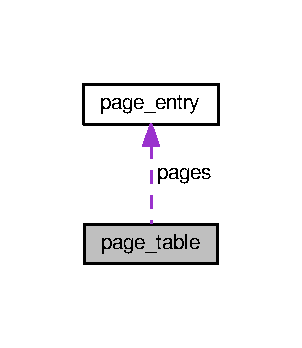
\includegraphics[width=145pt]{structpage__table__coll__graph}
\end{center}
\end{figure}
\subsection*{Data Fields}
\begin{DoxyCompactItemize}
\item 
\hyperlink{structpage__entry}{page\+\_\+entry} \hyperlink{structpage__table_aa066e0fa847ce2fafb6a2feddfa340ff}{pages} \mbox{[}1024\mbox{]}
\end{DoxyCompactItemize}


\subsection{Detailed Description}


Definition at line 26 of file paging.\+h.



\subsection{Field Documentation}
\index{page\+\_\+table@{page\+\_\+table}!pages@{pages}}
\index{pages@{pages}!page\+\_\+table@{page\+\_\+table}}
\subsubsection[{\texorpdfstring{pages}{pages}}]{\setlength{\rightskip}{0pt plus 5cm}{\bf page\+\_\+entry} page\+\_\+table\+::pages\mbox{[}1024\mbox{]}}\hypertarget{structpage__table_aa066e0fa847ce2fafb6a2feddfa340ff}{}\label{structpage__table_aa066e0fa847ce2fafb6a2feddfa340ff}


Definition at line 27 of file paging.\+h.



Referenced by get\+\_\+page().



The documentation for this struct was generated from the following file\+:\begin{DoxyCompactItemize}
\item 
/home/loudish/mpx-\/spring2017-\/modestus/mpx\+\_\+core/include/mem/\hyperlink{paging_8h}{paging.\+h}\end{DoxyCompactItemize}

\hypertarget{structparam}{}\section{param Struct Reference}
\label{structparam}\index{param@{param}}


{\ttfamily \#include $<$mpx\+\_\+supt.\+h$>$}

\subsection*{Data Fields}
\begin{DoxyCompactItemize}
\item 
int \hyperlink{structparam_a81c8b24055c2908ebe480598aba6044c}{op\+\_\+code}
\item 
int \hyperlink{structparam_a44a7285b02749114186a9f9971941bcb}{device\+\_\+id}
\end{DoxyCompactItemize}


\subsection{Detailed Description}


Definition at line 18 of file mpx\+\_\+supt.\+h.



\subsection{Field Documentation}
\index{param@{param}!device\+\_\+id@{device\+\_\+id}}
\index{device\+\_\+id@{device\+\_\+id}!param@{param}}
\subsubsection[{\texorpdfstring{device\+\_\+id}{device_id}}]{\setlength{\rightskip}{0pt plus 5cm}int param\+::device\+\_\+id}\hypertarget{structparam_a44a7285b02749114186a9f9971941bcb}{}\label{structparam_a44a7285b02749114186a9f9971941bcb}


Definition at line 20 of file mpx\+\_\+supt.\+h.

\index{param@{param}!op\+\_\+code@{op\+\_\+code}}
\index{op\+\_\+code@{op\+\_\+code}!param@{param}}
\subsubsection[{\texorpdfstring{op\+\_\+code}{op_code}}]{\setlength{\rightskip}{0pt plus 5cm}int param\+::op\+\_\+code}\hypertarget{structparam_a81c8b24055c2908ebe480598aba6044c}{}\label{structparam_a81c8b24055c2908ebe480598aba6044c}


Definition at line 19 of file mpx\+\_\+supt.\+h.



Referenced by sys\+\_\+req().



The documentation for this struct was generated from the following file\+:\begin{DoxyCompactItemize}
\item 
/home/loudish/mpx-\/spring2017-\/modestus/mpx\+\_\+core/include/core/\hyperlink{include_2core_2mpx__supt_8h}{mpx\+\_\+supt.\+h}\end{DoxyCompactItemize}

\hypertarget{structpcb__t}{}\section{pcb\+\_\+t Struct Reference}
\label{structpcb__t}\index{pcb\+\_\+t@{pcb\+\_\+t}}


typedef for \hyperlink{structpcb__t}{pcb\+\_\+t} struct  




{\ttfamily \#include $<$pcb$>$}



\subsection{Detailed Description}
typedef for \hyperlink{structpcb__t}{pcb\+\_\+t} struct 

\begin{DoxySeeAlso}{See also}
pcb\+\_\+struct\+\_\+t 
\end{DoxySeeAlso}


The documentation for this struct was generated from the following file\+:\begin{DoxyCompactItemize}
\item 
/home/loudish/mpx-\/spring2017-\/modestus/mpx\+\_\+core/include/core/\hyperlink{pcb_8h}{pcb.\+h}\end{DoxyCompactItemize}

\hypertarget{structs__pcb__stuct}{}\section{pcb\+\_\+t Struct Reference}
\label{structs__pcb__stuct}\index{pcb\+\_\+t@{pcb\+\_\+t}}


defines the properties of a process control block  




{\ttfamily \#include $<$pcb.\+h$>$}



Collaboration diagram for pcb\+\_\+t\+:\nopagebreak
\begin{figure}[H]
\begin{center}
\leavevmode
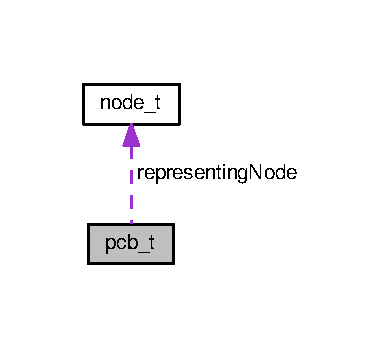
\includegraphics[width=183pt]{structs__pcb__stuct__coll__graph}
\end{center}
\end{figure}
\subsection*{Data Fields}
\begin{DoxyCompactItemize}
\item 
char \hyperlink{structs__pcb__stuct_a35c285b13db8c228686d0f8a6757df55}{name} \mbox{[}\hyperlink{pcb_8h_acd2dea966e4e5b760451b4fcc66f6cce}{P\+R\+O\+C\+E\+S\+S\+\_\+\+M\+A\+X\+\_\+\+N\+A\+M\+E\+\_\+\+L\+E\+N\+G\+TH}\mbox{]}
\item 
\hyperlink{pcb_8h_a679b474107b599ed5e2597c8863176dc}{P\+I\+D\+\_\+t} \hyperlink{structs__pcb__stuct_adb2bb17e9c8a673c566b6ca4abae4c3d}{P\+ID}
\item 
\hyperlink{system_8h_a7c94ea6f8948649f8d181ae55911eeaf}{size\+\_\+t} \hyperlink{structs__pcb__stuct_a55fc1faff03a8b63cf31bb2bfa23bdb3}{priority}
\item 
\hyperlink{pcb_8h_a8461d6c03c00b03bad59b5a29d27b902}{e\+\_\+\+P\+R\+O\+C\+E\+S\+S\+\_\+\+S\+T\+A\+T\+E\+\_\+t} \hyperlink{structs__pcb__stuct_a55061533a89faf41941be8e04f51166c}{process\+State}
\item 
\hyperlink{pcb_8h_ab3268ce0bdfc94e5757917d42c73d9f1}{e\+\_\+\+P\+R\+O\+C\+E\+S\+S\+\_\+\+C\+L\+A\+S\+S\+\_\+t} \hyperlink{structs__pcb__stuct_a3b2308e186f613a782a1da4a798ef73b}{process\+Class}
\item 
\hyperlink{system_8h_a7c94ea6f8948649f8d181ae55911eeaf}{size\+\_\+t} \hyperlink{structs__pcb__stuct_a54d339e4c45de597429888e4654c03c8}{context} \mbox{[}\hyperlink{pcb_8h_abb5f1eb47c3ac477582ecc49dc8990ee}{P\+R\+O\+C\+E\+S\+S\+\_\+\+C\+O\+N\+T\+E\+X\+T\+\_\+\+S\+I\+ZE}\mbox{]}
\item 
\hyperlink{pcb_8h_aeac19486a8c4d8375298127cee4305b1}{program\+Ptr\+\_\+t} $\ast$ \hyperlink{structs__pcb__stuct_aa3a3020774ef77f1de4de8dd23d78743}{program\+Start}
\item 
\hyperlink{system_8h_a7c94ea6f8948649f8d181ae55911eeaf}{size\+\_\+t} \hyperlink{structs__pcb__stuct_a18647991a99249b0a51f30ee6004a81c}{program\+Size}
\item 
\hyperlink{pcb_8h_a4f8494f06fbe4ad011320128964be020}{program\+Data\+Ptr\+\_\+t} $\ast$ \hyperlink{structs__pcb__stuct_ac5d905bfc91bb5364487b48fe06a7fc2}{data\+Start}
\item 
\hyperlink{system_8h_a7c94ea6f8948649f8d181ae55911eeaf}{size\+\_\+t} \hyperlink{structs__pcb__stuct_aaaf251e1893020160fb154a5e341f604}{data\+Size}
\item 
\hyperlink{pcb_8h_a39f696168968032d4df0637fad2ad52c}{process\+Stack\+\_\+t} $\ast$ \hyperlink{structs__pcb__stuct_aec0fa5de5c09ee7db1da3b953af71321}{stack\+Bottom}
\item 
\hyperlink{pcb_8h_a39f696168968032d4df0637fad2ad52c}{process\+Stack\+\_\+t} $\ast$ \hyperlink{structs__pcb__stuct_a3fd35f3889ce588dc9af9b0c74fd2db9}{stack\+Base}
\item 
\hyperlink{pcb_8h_a39f696168968032d4df0637fad2ad52c}{process\+Stack\+\_\+t} $\ast$ \hyperlink{structs__pcb__stuct_a8ea780f48f7f2a4f9e337abaf510896e}{stack\+Top}
\item 
\hyperlink{structnode__t}{node\+\_\+t} $\ast$ \hyperlink{structs__pcb__stuct_a56fe193ec1b8061c850d79247bccb98d}{representing\+Node}
\end{DoxyCompactItemize}


\subsection{Detailed Description}
defines the properties of a process control block 

Definition at line 87 of file pcb.\+h.



\subsection{Field Documentation}
\index{s\+\_\+pcb\+\_\+stuct@{s\+\_\+pcb\+\_\+stuct}!context@{context}}
\index{context@{context}!s\+\_\+pcb\+\_\+stuct@{s\+\_\+pcb\+\_\+stuct}}
\subsubsection[{\texorpdfstring{context}{context}}]{\setlength{\rightskip}{0pt plus 5cm}{\bf size\+\_\+t} pcb\+\_\+t\+::context\mbox{[}{\bf P\+R\+O\+C\+E\+S\+S\+\_\+\+C\+O\+N\+T\+E\+X\+T\+\_\+\+S\+I\+ZE}\mbox{]}}\hypertarget{structs__pcb__stuct_a54d339e4c45de597429888e4654c03c8}{}\label{structs__pcb__stuct_a54d339e4c45de597429888e4654c03c8}


Definition at line 96 of file pcb.\+h.

\index{s\+\_\+pcb\+\_\+stuct@{s\+\_\+pcb\+\_\+stuct}!data\+Size@{data\+Size}}
\index{data\+Size@{data\+Size}!s\+\_\+pcb\+\_\+stuct@{s\+\_\+pcb\+\_\+stuct}}
\subsubsection[{\texorpdfstring{data\+Size}{dataSize}}]{\setlength{\rightskip}{0pt plus 5cm}{\bf size\+\_\+t} pcb\+\_\+t\+::data\+Size}\hypertarget{structs__pcb__stuct_aaaf251e1893020160fb154a5e341f604}{}\label{structs__pcb__stuct_aaaf251e1893020160fb154a5e341f604}


Definition at line 104 of file pcb.\+h.

\index{s\+\_\+pcb\+\_\+stuct@{s\+\_\+pcb\+\_\+stuct}!data\+Start@{data\+Start}}
\index{data\+Start@{data\+Start}!s\+\_\+pcb\+\_\+stuct@{s\+\_\+pcb\+\_\+stuct}}
\subsubsection[{\texorpdfstring{data\+Start}{dataStart}}]{\setlength{\rightskip}{0pt plus 5cm}{\bf program\+Data\+Ptr\+\_\+t}$\ast$ pcb\+\_\+t\+::data\+Start}\hypertarget{structs__pcb__stuct_ac5d905bfc91bb5364487b48fe06a7fc2}{}\label{structs__pcb__stuct_ac5d905bfc91bb5364487b48fe06a7fc2}


Definition at line 103 of file pcb.\+h.

\index{s\+\_\+pcb\+\_\+stuct@{s\+\_\+pcb\+\_\+stuct}!name@{name}}
\index{name@{name}!s\+\_\+pcb\+\_\+stuct@{s\+\_\+pcb\+\_\+stuct}}
\subsubsection[{\texorpdfstring{name}{name}}]{\setlength{\rightskip}{0pt plus 5cm}char pcb\+\_\+t\+::name\mbox{[}{\bf P\+R\+O\+C\+E\+S\+S\+\_\+\+M\+A\+X\+\_\+\+N\+A\+M\+E\+\_\+\+L\+E\+N\+G\+TH}\mbox{]}}\hypertarget{structs__pcb__stuct_a35c285b13db8c228686d0f8a6757df55}{}\label{structs__pcb__stuct_a35c285b13db8c228686d0f8a6757df55}


Definition at line 89 of file pcb.\+h.

\index{s\+\_\+pcb\+\_\+stuct@{s\+\_\+pcb\+\_\+stuct}!P\+ID@{P\+ID}}
\index{P\+ID@{P\+ID}!s\+\_\+pcb\+\_\+stuct@{s\+\_\+pcb\+\_\+stuct}}
\subsubsection[{\texorpdfstring{P\+ID}{PID}}]{\setlength{\rightskip}{0pt plus 5cm}{\bf P\+I\+D\+\_\+t} pcb\+\_\+t\+::\+P\+ID}\hypertarget{structs__pcb__stuct_adb2bb17e9c8a673c566b6ca4abae4c3d}{}\label{structs__pcb__stuct_adb2bb17e9c8a673c566b6ca4abae4c3d}


Definition at line 90 of file pcb.\+h.

\index{s\+\_\+pcb\+\_\+stuct@{s\+\_\+pcb\+\_\+stuct}!priority@{priority}}
\index{priority@{priority}!s\+\_\+pcb\+\_\+stuct@{s\+\_\+pcb\+\_\+stuct}}
\subsubsection[{\texorpdfstring{priority}{priority}}]{\setlength{\rightskip}{0pt plus 5cm}{\bf size\+\_\+t} pcb\+\_\+t\+::priority}\hypertarget{structs__pcb__stuct_a55fc1faff03a8b63cf31bb2bfa23bdb3}{}\label{structs__pcb__stuct_a55fc1faff03a8b63cf31bb2bfa23bdb3}


Definition at line 91 of file pcb.\+h.

\index{s\+\_\+pcb\+\_\+stuct@{s\+\_\+pcb\+\_\+stuct}!process\+Class@{process\+Class}}
\index{process\+Class@{process\+Class}!s\+\_\+pcb\+\_\+stuct@{s\+\_\+pcb\+\_\+stuct}}
\subsubsection[{\texorpdfstring{process\+Class}{processClass}}]{\setlength{\rightskip}{0pt plus 5cm}{\bf e\+\_\+\+P\+R\+O\+C\+E\+S\+S\+\_\+\+C\+L\+A\+S\+S\+\_\+t} pcb\+\_\+t\+::process\+Class}\hypertarget{structs__pcb__stuct_a3b2308e186f613a782a1da4a798ef73b}{}\label{structs__pcb__stuct_a3b2308e186f613a782a1da4a798ef73b}


Definition at line 94 of file pcb.\+h.

\index{s\+\_\+pcb\+\_\+stuct@{s\+\_\+pcb\+\_\+stuct}!process\+State@{process\+State}}
\index{process\+State@{process\+State}!s\+\_\+pcb\+\_\+stuct@{s\+\_\+pcb\+\_\+stuct}}
\subsubsection[{\texorpdfstring{process\+State}{processState}}]{\setlength{\rightskip}{0pt plus 5cm}{\bf e\+\_\+\+P\+R\+O\+C\+E\+S\+S\+\_\+\+S\+T\+A\+T\+E\+\_\+t} pcb\+\_\+t\+::process\+State}\hypertarget{structs__pcb__stuct_a55061533a89faf41941be8e04f51166c}{}\label{structs__pcb__stuct_a55061533a89faf41941be8e04f51166c}


Definition at line 93 of file pcb.\+h.

\index{s\+\_\+pcb\+\_\+stuct@{s\+\_\+pcb\+\_\+stuct}!program\+Size@{program\+Size}}
\index{program\+Size@{program\+Size}!s\+\_\+pcb\+\_\+stuct@{s\+\_\+pcb\+\_\+stuct}}
\subsubsection[{\texorpdfstring{program\+Size}{programSize}}]{\setlength{\rightskip}{0pt plus 5cm}{\bf size\+\_\+t} pcb\+\_\+t\+::program\+Size}\hypertarget{structs__pcb__stuct_a18647991a99249b0a51f30ee6004a81c}{}\label{structs__pcb__stuct_a18647991a99249b0a51f30ee6004a81c}


Definition at line 101 of file pcb.\+h.

\index{s\+\_\+pcb\+\_\+stuct@{s\+\_\+pcb\+\_\+stuct}!program\+Start@{program\+Start}}
\index{program\+Start@{program\+Start}!s\+\_\+pcb\+\_\+stuct@{s\+\_\+pcb\+\_\+stuct}}
\subsubsection[{\texorpdfstring{program\+Start}{programStart}}]{\setlength{\rightskip}{0pt plus 5cm}{\bf program\+Ptr\+\_\+t}$\ast$ pcb\+\_\+t\+::program\+Start}\hypertarget{structs__pcb__stuct_aa3a3020774ef77f1de4de8dd23d78743}{}\label{structs__pcb__stuct_aa3a3020774ef77f1de4de8dd23d78743}


Definition at line 100 of file pcb.\+h.

\index{s\+\_\+pcb\+\_\+stuct@{s\+\_\+pcb\+\_\+stuct}!representing\+Node@{representing\+Node}}
\index{representing\+Node@{representing\+Node}!s\+\_\+pcb\+\_\+stuct@{s\+\_\+pcb\+\_\+stuct}}
\subsubsection[{\texorpdfstring{representing\+Node}{representingNode}}]{\setlength{\rightskip}{0pt plus 5cm}{\bf node\+\_\+t}$\ast$ pcb\+\_\+t\+::representing\+Node}\hypertarget{structs__pcb__stuct_a56fe193ec1b8061c850d79247bccb98d}{}\label{structs__pcb__stuct_a56fe193ec1b8061c850d79247bccb98d}


Definition at line 110 of file pcb.\+h.

\index{s\+\_\+pcb\+\_\+stuct@{s\+\_\+pcb\+\_\+stuct}!stack\+Base@{stack\+Base}}
\index{stack\+Base@{stack\+Base}!s\+\_\+pcb\+\_\+stuct@{s\+\_\+pcb\+\_\+stuct}}
\subsubsection[{\texorpdfstring{stack\+Base}{stackBase}}]{\setlength{\rightskip}{0pt plus 5cm}{\bf process\+Stack\+\_\+t}$\ast$ pcb\+\_\+t\+::stack\+Base}\hypertarget{structs__pcb__stuct_a3fd35f3889ce588dc9af9b0c74fd2db9}{}\label{structs__pcb__stuct_a3fd35f3889ce588dc9af9b0c74fd2db9}


Definition at line 107 of file pcb.\+h.

\index{s\+\_\+pcb\+\_\+stuct@{s\+\_\+pcb\+\_\+stuct}!stack\+Bottom@{stack\+Bottom}}
\index{stack\+Bottom@{stack\+Bottom}!s\+\_\+pcb\+\_\+stuct@{s\+\_\+pcb\+\_\+stuct}}
\subsubsection[{\texorpdfstring{stack\+Bottom}{stackBottom}}]{\setlength{\rightskip}{0pt plus 5cm}{\bf process\+Stack\+\_\+t}$\ast$ pcb\+\_\+t\+::stack\+Bottom}\hypertarget{structs__pcb__stuct_aec0fa5de5c09ee7db1da3b953af71321}{}\label{structs__pcb__stuct_aec0fa5de5c09ee7db1da3b953af71321}


Definition at line 106 of file pcb.\+h.

\index{s\+\_\+pcb\+\_\+stuct@{s\+\_\+pcb\+\_\+stuct}!stack\+Top@{stack\+Top}}
\index{stack\+Top@{stack\+Top}!s\+\_\+pcb\+\_\+stuct@{s\+\_\+pcb\+\_\+stuct}}
\subsubsection[{\texorpdfstring{stack\+Top}{stackTop}}]{\setlength{\rightskip}{0pt plus 5cm}{\bf process\+Stack\+\_\+t}$\ast$ pcb\+\_\+t\+::stack\+Top}\hypertarget{structs__pcb__stuct_a8ea780f48f7f2a4f9e337abaf510896e}{}\label{structs__pcb__stuct_a8ea780f48f7f2a4f9e337abaf510896e}


Definition at line 108 of file pcb.\+h.



The documentation for this struct was generated from the following file\+:\begin{DoxyCompactItemize}
\item 
/home/loudish/mpx-\/spring2017-\/modestus/mpx\+\_\+core/include/core/\hyperlink{pcb_8h}{pcb.\+h}\end{DoxyCompactItemize}

\hypertarget{structpcb_queue__t}{}\section{pcb\+Queue\+\_\+t Struct Reference}
\label{structpcb_queue__t}\index{pcb\+Queue\+\_\+t@{pcb\+Queue\+\_\+t}}


typedef for \hyperlink{structpcb_queue__t}{pcb\+Queue\+\_\+t} struct  




{\ttfamily \#include $<$pcb$>$}



\subsection{Detailed Description}
typedef for \hyperlink{structpcb_queue__t}{pcb\+Queue\+\_\+t} struct 

\begin{DoxySeeAlso}{See also}
s\+\_\+pcb\+\_\+list 
\end{DoxySeeAlso}


The documentation for this struct was generated from the following file\+:\begin{DoxyCompactItemize}
\item 
/home/loudish/mpx-\/spring2017-\/modestus/mpx\+\_\+core/include/core/\hyperlink{pcb_8h}{pcb.\+h}\end{DoxyCompactItemize}

\chapter{File Documentation}
\hypertarget{arg__list_8h}{}\section{/home/loudish/mpx-\/spring2017-\/modestus/mpx\+\_\+core/include/arg\+\_\+list.h File Reference}
\label{arg__list_8h}\index{/home/loudish/mpx-\/spring2017-\/modestus/mpx\+\_\+core/include/arg\+\_\+list.\+h@{/home/loudish/mpx-\/spring2017-\/modestus/mpx\+\_\+core/include/arg\+\_\+list.\+h}}
This graph shows which files directly or indirectly include this file\+:\nopagebreak
\begin{figure}[H]
\begin{center}
\leavevmode
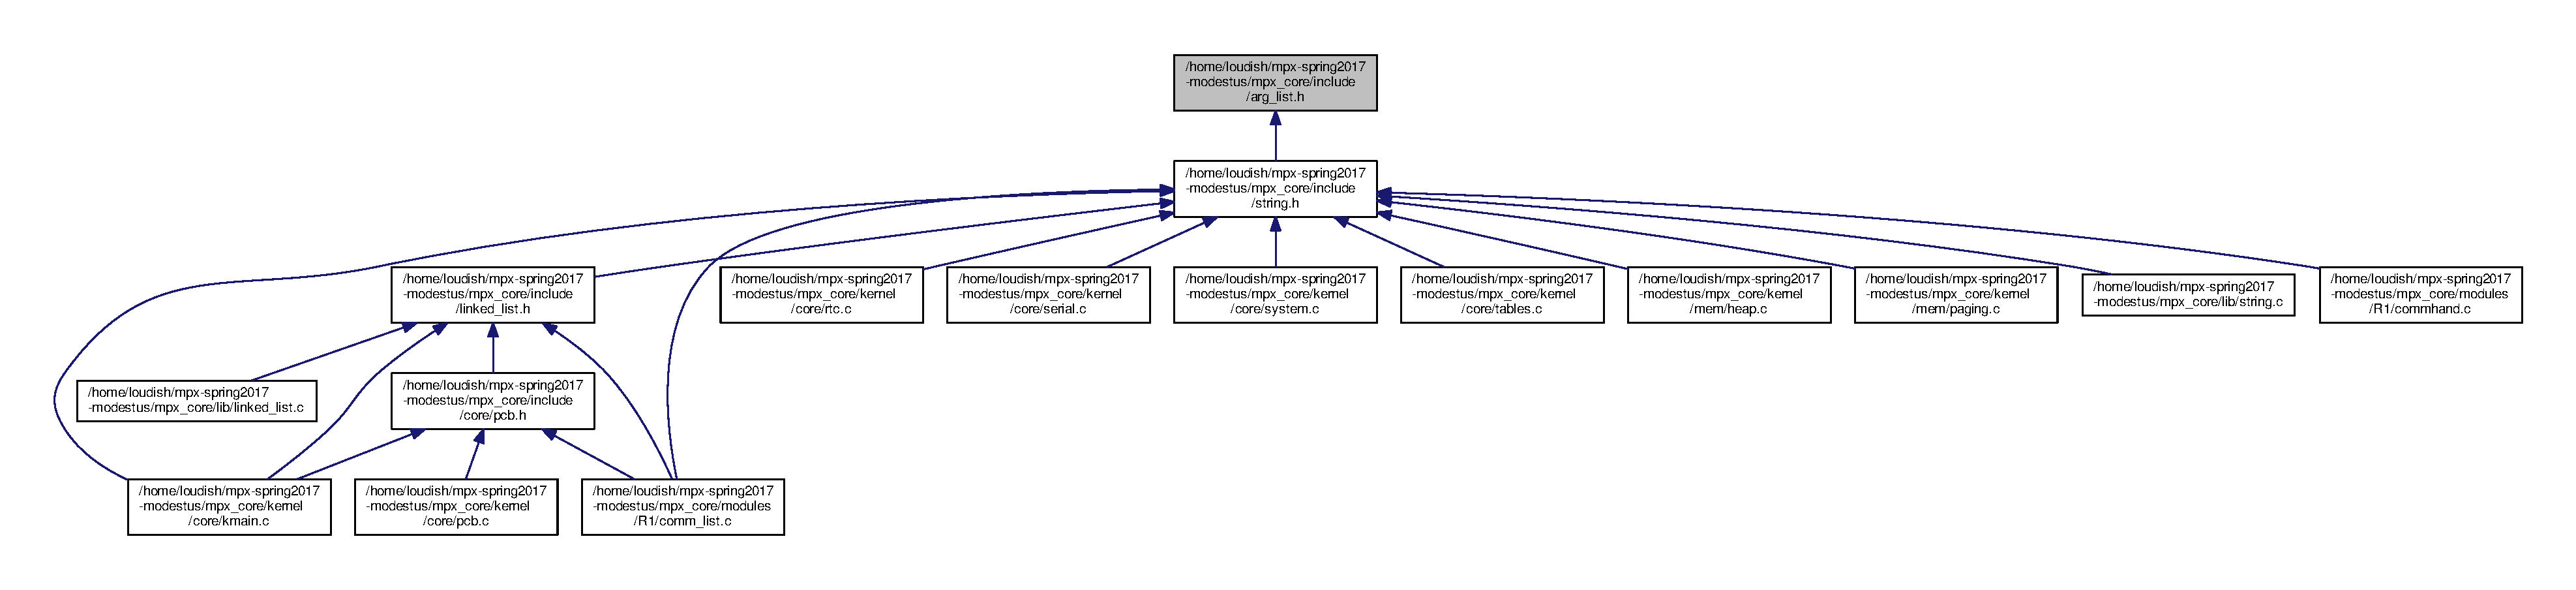
\includegraphics[width=350pt]{arg__list_8h__dep__incl}
\end{center}
\end{figure}
\subsection*{Macros}
\begin{DoxyCompactItemize}
\item 
\#define \hyperlink{arg__list_8h_abb821de0a9df92f33d827f2008093ddc}{arg\+\_\+list}~unsigned char$\ast$
\item 
\#define \hyperlink{arg__list_8h_a65f99a627ef400f9d875acca35dbac69}{init\+\_\+arg\+\_\+list}(arg\+List,  arg\+Before\+Ellipses)
\begin{DoxyCompactList}\small\item\em implemented in macro because there are no templates in C \end{DoxyCompactList}\end{DoxyCompactItemize}


\subsection{Macro Definition Documentation}
\index{arg\+\_\+list.\+h@{arg\+\_\+list.\+h}!arg\+\_\+list@{arg\+\_\+list}}
\index{arg\+\_\+list@{arg\+\_\+list}!arg\+\_\+list.\+h@{arg\+\_\+list.\+h}}
\subsubsection[{\texorpdfstring{arg\+\_\+list}{arg_list}}]{\setlength{\rightskip}{0pt plus 5cm}\#define arg\+\_\+list~unsigned char$\ast$}\hypertarget{arg__list_8h_abb821de0a9df92f33d827f2008093ddc}{}\label{arg__list_8h_abb821de0a9df92f33d827f2008093ddc}
arg\+\_\+list maintatins a pointer to the current argument on the stack 

Definition at line 19 of file arg\+\_\+list.\+h.



Referenced by \+\_\+\+\_\+attribute\+\_\+\+\_\+().

\index{arg\+\_\+list.\+h@{arg\+\_\+list.\+h}!init\+\_\+arg\+\_\+list@{init\+\_\+arg\+\_\+list}}
\index{init\+\_\+arg\+\_\+list@{init\+\_\+arg\+\_\+list}!arg\+\_\+list.\+h@{arg\+\_\+list.\+h}}
\subsubsection[{\texorpdfstring{init\+\_\+arg\+\_\+list}{init_arg_list}}]{\setlength{\rightskip}{0pt plus 5cm}\#define init\+\_\+arg\+\_\+list(
\begin{DoxyParamCaption}
\item[{}]{arg\+List, }
\item[{}]{arg\+Before\+Ellipses}
\end{DoxyParamCaption}
)}\hypertarget{arg__list_8h_a65f99a627ef400f9d875acca35dbac69}{}\label{arg__list_8h_a65f99a627ef400f9d875acca35dbac69}
{\bfseries Value\+:}
\begin{DoxyCode}
\{ \(\backslash\)
        argList = (\textcolor{keywordtype}{unsigned} \textcolor{keywordtype}{char}*)&argBeforeEllipses; \(\backslash\)
    \} \(\backslash\)
\end{DoxyCode}


implemented in macro because there are no templates in C 

input args are an arg\+\_\+list, and the last argument of a variadic function 

Definition at line 25 of file arg\+\_\+list.\+h.



Referenced by \+\_\+\+\_\+attribute\+\_\+\+\_\+().


\hypertarget{comm__vars_8h}{}\section{/home/loudish/mpx-\/spring2017-\/modestus/mpx\+\_\+core/include/comm\+\_\+vars.h File Reference}
\label{comm__vars_8h}\index{/home/loudish/mpx-\/spring2017-\/modestus/mpx\+\_\+core/include/comm\+\_\+vars.\+h@{/home/loudish/mpx-\/spring2017-\/modestus/mpx\+\_\+core/include/comm\+\_\+vars.\+h}}
This graph shows which files directly or indirectly include this file\+:\nopagebreak
\begin{figure}[H]
\begin{center}
\leavevmode
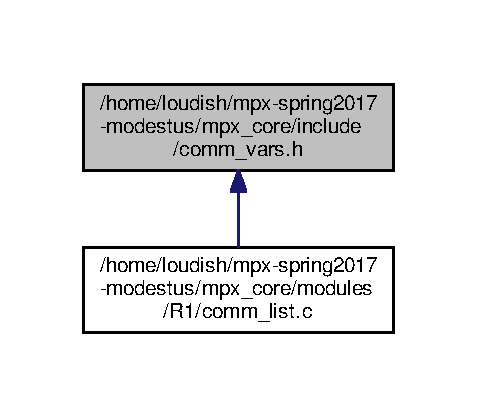
\includegraphics[width=229pt]{comm__vars_8h__dep__incl}
\end{center}
\end{figure}
\subsection*{Macros}
\begin{DoxyCompactItemize}
\item 
\#define \hyperlink{comm__vars_8h_a1c6d5de492ac61ad29aec7aa9a436bbf}{V\+E\+R\+S\+I\+ON}~\char`\"{}R1\char`\"{}
\item 
\#define \hyperlink{comm__vars_8h_adc0c870b429ed41ab22e23dbba9e6af1}{I\+M\+P\+R\+O\+P\+E\+R\+\_\+\+C\+O\+M\+M\+A\+ND}~\char`\"{}That is not a proper command.  Type \textquotesingle{}\hyperlink{comm__list_8h_a97ee70a8770dc30d06c744b24eb2fcfc}{help}\textquotesingle{} to see a list of commands.\char`\"{}
\item 
\#define \hyperlink{comm__vars_8h_ac5f4cf1c989af592617184f7a7e5c372}{U\+N\+K\+N\+O\+W\+N\+\_\+\+C\+O\+M\+M\+A\+ND}~\char`\"{}U\+N\+K\+O\+WN C\+O\+M\+M\+A\+ND, type \textquotesingle{}\hyperlink{comm__list_8h_a97ee70a8770dc30d06c744b24eb2fcfc}{help}\textquotesingle{} to see a list of commands and arguments.\char`\"{}
\item 
\#define \hyperlink{comm__vars_8h_a3d75ee5ce40f6fc7b3182661c2e11fde}{E\+X\+T\+R\+A\+\_\+\+P\+A\+R\+A\+M\+E\+T\+E\+RS}~\char`\"{}Extra parameter found\+: \char`\"{}
\end{DoxyCompactItemize}


\subsection{Macro Definition Documentation}
\index{comm\+\_\+vars.\+h@{comm\+\_\+vars.\+h}!E\+X\+T\+R\+A\+\_\+\+P\+A\+R\+A\+M\+E\+T\+E\+RS@{E\+X\+T\+R\+A\+\_\+\+P\+A\+R\+A\+M\+E\+T\+E\+RS}}
\index{E\+X\+T\+R\+A\+\_\+\+P\+A\+R\+A\+M\+E\+T\+E\+RS@{E\+X\+T\+R\+A\+\_\+\+P\+A\+R\+A\+M\+E\+T\+E\+RS}!comm\+\_\+vars.\+h@{comm\+\_\+vars.\+h}}
\subsubsection[{\texorpdfstring{E\+X\+T\+R\+A\+\_\+\+P\+A\+R\+A\+M\+E\+T\+E\+RS}{EXTRA_PARAMETERS}}]{\setlength{\rightskip}{0pt plus 5cm}\#define E\+X\+T\+R\+A\+\_\+\+P\+A\+R\+A\+M\+E\+T\+E\+RS~\char`\"{}Extra parameter found\+: \char`\"{}}\hypertarget{comm__vars_8h_a3d75ee5ce40f6fc7b3182661c2e11fde}{}\label{comm__vars_8h_a3d75ee5ce40f6fc7b3182661c2e11fde}


Definition at line 4 of file comm\+\_\+vars.\+h.



Referenced by pcb\+Func().

\index{comm\+\_\+vars.\+h@{comm\+\_\+vars.\+h}!I\+M\+P\+R\+O\+P\+E\+R\+\_\+\+C\+O\+M\+M\+A\+ND@{I\+M\+P\+R\+O\+P\+E\+R\+\_\+\+C\+O\+M\+M\+A\+ND}}
\index{I\+M\+P\+R\+O\+P\+E\+R\+\_\+\+C\+O\+M\+M\+A\+ND@{I\+M\+P\+R\+O\+P\+E\+R\+\_\+\+C\+O\+M\+M\+A\+ND}!comm\+\_\+vars.\+h@{comm\+\_\+vars.\+h}}
\subsubsection[{\texorpdfstring{I\+M\+P\+R\+O\+P\+E\+R\+\_\+\+C\+O\+M\+M\+A\+ND}{IMPROPER_COMMAND}}]{\setlength{\rightskip}{0pt plus 5cm}\#define I\+M\+P\+R\+O\+P\+E\+R\+\_\+\+C\+O\+M\+M\+A\+ND~\char`\"{}That is not a proper command.  Type \textquotesingle{}{\bf help}\textquotesingle{} to see a list of commands.\char`\"{}}\hypertarget{comm__vars_8h_adc0c870b429ed41ab22e23dbba9e6af1}{}\label{comm__vars_8h_adc0c870b429ed41ab22e23dbba9e6af1}


Definition at line 2 of file comm\+\_\+vars.\+h.



Referenced by help\+Func(), set\+Date(), and set\+Time().

\index{comm\+\_\+vars.\+h@{comm\+\_\+vars.\+h}!U\+N\+K\+N\+O\+W\+N\+\_\+\+C\+O\+M\+M\+A\+ND@{U\+N\+K\+N\+O\+W\+N\+\_\+\+C\+O\+M\+M\+A\+ND}}
\index{U\+N\+K\+N\+O\+W\+N\+\_\+\+C\+O\+M\+M\+A\+ND@{U\+N\+K\+N\+O\+W\+N\+\_\+\+C\+O\+M\+M\+A\+ND}!comm\+\_\+vars.\+h@{comm\+\_\+vars.\+h}}
\subsubsection[{\texorpdfstring{U\+N\+K\+N\+O\+W\+N\+\_\+\+C\+O\+M\+M\+A\+ND}{UNKNOWN_COMMAND}}]{\setlength{\rightskip}{0pt plus 5cm}\#define U\+N\+K\+N\+O\+W\+N\+\_\+\+C\+O\+M\+M\+A\+ND~\char`\"{}U\+N\+K\+O\+WN C\+O\+M\+M\+A\+ND, type \textquotesingle{}{\bf help}\textquotesingle{} to see a list of commands and arguments.\char`\"{}}\hypertarget{comm__vars_8h_ac5f4cf1c989af592617184f7a7e5c372}{}\label{comm__vars_8h_ac5f4cf1c989af592617184f7a7e5c372}


Definition at line 3 of file comm\+\_\+vars.\+h.

\index{comm\+\_\+vars.\+h@{comm\+\_\+vars.\+h}!V\+E\+R\+S\+I\+ON@{V\+E\+R\+S\+I\+ON}}
\index{V\+E\+R\+S\+I\+ON@{V\+E\+R\+S\+I\+ON}!comm\+\_\+vars.\+h@{comm\+\_\+vars.\+h}}
\subsubsection[{\texorpdfstring{V\+E\+R\+S\+I\+ON}{VERSION}}]{\setlength{\rightskip}{0pt plus 5cm}\#define V\+E\+R\+S\+I\+ON~\char`\"{}R1\char`\"{}}\hypertarget{comm__vars_8h_a1c6d5de492ac61ad29aec7aa9a436bbf}{}\label{comm__vars_8h_a1c6d5de492ac61ad29aec7aa9a436bbf}


Definition at line 1 of file comm\+\_\+vars.\+h.



Referenced by version().


\hypertarget{anim_8h}{}\section{/home/loudish/mpx-\/spring2017-\/modestus/mpx\+\_\+core/include/core/anim.h File Reference}
\label{anim_8h}\index{/home/loudish/mpx-\/spring2017-\/modestus/mpx\+\_\+core/include/core/anim.\+h@{/home/loudish/mpx-\/spring2017-\/modestus/mpx\+\_\+core/include/core/anim.\+h}}
This graph shows which files directly or indirectly include this file\+:\nopagebreak
\begin{figure}[H]
\begin{center}
\leavevmode
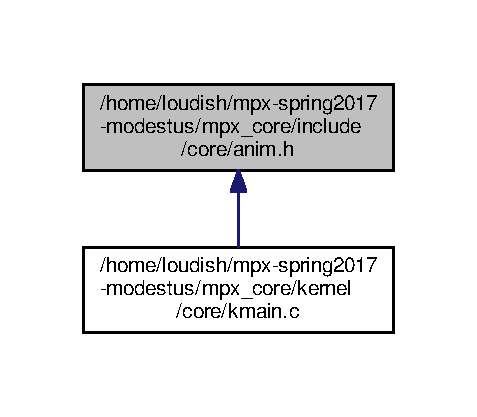
\includegraphics[width=229pt]{anim_8h__dep__incl}
\end{center}
\end{figure}
\subsection*{Functions}
\begin{DoxyCompactItemize}
\item 
void \hyperlink{anim_8h_a5bf31d96ce4c2c86dfab5440a835c457}{start\+\_\+up\+\_\+anim} (void)
\item 
void \hyperlink{anim_8h_accd23e11967f6634e7885688e395b964}{busy\+\_\+wait} (void)
\item 
void \hyperlink{anim_8h_abc40cd622f423abf44084c8f8595f57f}{clear\+\_\+screen} (void)
\end{DoxyCompactItemize}


\subsection{Function Documentation}
\index{anim.\+h@{anim.\+h}!busy\+\_\+wait@{busy\+\_\+wait}}
\index{busy\+\_\+wait@{busy\+\_\+wait}!anim.\+h@{anim.\+h}}
\subsubsection[{\texorpdfstring{busy\+\_\+wait(void)}{busy_wait(void)}}]{\setlength{\rightskip}{0pt plus 5cm}void busy\+\_\+wait (
\begin{DoxyParamCaption}
\item[{void}]{}
\end{DoxyParamCaption}
)}\hypertarget{anim_8h_accd23e11967f6634e7885688e395b964}{}\label{anim_8h_accd23e11967f6634e7885688e395b964}
R\+E-\/\+W\+R\+I\+TE T\+H\+IS SO T\+H\+AT IS IS M\+O\+RE E\+F\+F\+I\+C\+I\+E\+NT R\+U\+N\+N\+I\+NG 9999999 A\+SM C\+A\+L\+LS TO W\+A\+IT IS D\+U\+MB I\+N\+T\+E\+R\+R\+U\+P\+TS OR C\+H\+E\+CK T\+I\+ME W\+O\+U\+LD BE B\+E\+T\+T\+ER 

Definition at line 10 of file anim.\+c.



Referenced by start\+\_\+up\+\_\+anim().


\begin{DoxyCode}
10                  \{
11     \textcolor{keywordtype}{int} i = 0;
12     \textcolor{keywordflow}{for} (; i < 9999999; i++) \{
13         \textcolor{keyword}{asm} \textcolor{keyword}{volatile}(\textcolor{stringliteral}{"nop"});
14     \}
15 \}
\end{DoxyCode}
\index{anim.\+h@{anim.\+h}!clear\+\_\+screen@{clear\+\_\+screen}}
\index{clear\+\_\+screen@{clear\+\_\+screen}!anim.\+h@{anim.\+h}}
\subsubsection[{\texorpdfstring{clear\+\_\+screen(void)}{clear_screen(void)}}]{\setlength{\rightskip}{0pt plus 5cm}void clear\+\_\+screen (
\begin{DoxyParamCaption}
\item[{void}]{}
\end{DoxyParamCaption}
)}\hypertarget{anim_8h_abc40cd622f423abf44084c8f8595f57f}{}\label{anim_8h_abc40cd622f423abf44084c8f8595f57f}


Definition at line 17 of file anim.\+c.



References serial\+\_\+println().



Referenced by start\+\_\+up\+\_\+anim().


\begin{DoxyCode}
17                     \{
18     \hyperlink{serial_8h_a3514f7abff236a4e00a6c46021ce5e22}{serial\_println}(\textcolor{stringliteral}{"\(\backslash\)033[2J"});
19 \}
\end{DoxyCode}
\index{anim.\+h@{anim.\+h}!start\+\_\+up\+\_\+anim@{start\+\_\+up\+\_\+anim}}
\index{start\+\_\+up\+\_\+anim@{start\+\_\+up\+\_\+anim}!anim.\+h@{anim.\+h}}
\subsubsection[{\texorpdfstring{start\+\_\+up\+\_\+anim(void)}{start_up_anim(void)}}]{\setlength{\rightskip}{0pt plus 5cm}void start\+\_\+up\+\_\+anim (
\begin{DoxyParamCaption}
\item[{void}]{}
\end{DoxyParamCaption}
)}\hypertarget{anim_8h_a5bf31d96ce4c2c86dfab5440a835c457}{}\label{anim_8h_a5bf31d96ce4c2c86dfab5440a835c457}


Definition at line 21 of file anim.\+c.



References busy\+\_\+wait(), clear\+\_\+screen(), and serial\+\_\+println().



Referenced by kmain().


\begin{DoxyCode}
21                      \{
22     \hyperlink{serial_8h_a3514f7abff236a4e00a6c46021ce5e22}{serial\_println}(\textcolor{stringliteral}{"                 .------------.                                        "})
      ;
23     \hyperlink{serial_8h_a3514f7abff236a4e00a6c46021ce5e22}{serial\_println}(\textcolor{stringliteral}{"             .--'  o     . .   `--.                                "});
24     \hyperlink{serial_8h_a3514f7abff236a4e00a6c46021ce5e22}{serial\_println}(\textcolor{stringliteral}{"          .-'   .    O   .       . `-.                             "});
25     \hyperlink{serial_8h_a3514f7abff236a4e00a6c46021ce5e22}{serial\_println}(\textcolor{stringliteral}{"       .-'@   @@@@@@@   .  @@@@@      `-.                          "});
26     \hyperlink{serial_8h_a3514f7abff236a4e00a6c46021ce5e22}{serial\_println}(\textcolor{stringliteral}{"      /@@@  @@@@@@@@@@@   @@@@@@@   .    \(\backslash\)\(\backslash\)                        "});
27     \hyperlink{serial_8h_a3514f7abff236a4e00a6c46021ce5e22}{serial\_println}(\textcolor{stringliteral}{"    ./    o @@@@@@@@@@@   @@@@@@@       . \(\backslash\)\(\backslash\).                      "});
28     \hyperlink{serial_8h_a3514f7abff236a4e00a6c46021ce5e22}{serial\_println}(\textcolor{stringliteral}{"   /@@  o   @@@@@@@@@@@.   @@@@@@@   O      \(\backslash\)\(\backslash\)                     "});
29     \hyperlink{serial_8h_a3514f7abff236a4e00a6c46021ce5e22}{serial\_println}(\textcolor{stringliteral}{"  /@@@@   .   @@@@@@@o    @@@@@@@@@@     @@@ \(\backslash\)\(\backslash\)                    "});
30     \hyperlink{serial_8h_a3514f7abff236a4e00a6c46021ce5e22}{serial\_println}(\textcolor{stringliteral}{"  |@@@@@               . @@@@@@@@@@@@@ o @@@@|                     "});
31     \hyperlink{serial_8h_a3514f7abff236a4e00a6c46021ce5e22}{serial\_println}(\textcolor{stringliteral}{" /@@@@@  O  `.-./  .      @@@@@@@@@@@@    @@  \(\backslash\)\(\backslash\)                   "});
32     \hyperlink{serial_8h_a3514f7abff236a4e00a6c46021ce5e22}{serial\_println}(\textcolor{stringliteral}{" | @@@@    --`-'       o     @@@@@@@@ @@@@    |                   "});
33     \hyperlink{serial_8h_a3514f7abff236a4e00a6c46021ce5e22}{serial\_println}(\textcolor{stringliteral}{" |@ @@@        `    o      .  @@   . @@@@@@@  |                    "});
34     \hyperlink{serial_8h_a3514f7abff236a4e00a6c46021ce5e22}{serial\_println}(\textcolor{stringliteral}{" |       @@  @         .-.     @@@   @@@@@@@  |                   "});
35     \hyperlink{serial_8h_a3514f7abff236a4e00a6c46021ce5e22}{serial\_println}(\textcolor{stringliteral}{" \(\backslash\)\(\backslash\)  . @        @@@     `-'   . @@@@   @@@@  o /                   "});
36     \hyperlink{serial_8h_a3514f7abff236a4e00a6c46021ce5e22}{serial\_println}(\textcolor{stringliteral}{"  |      @@   @@@@@ .           @@   .       |                     "});
37     \hyperlink{serial_8h_a3514f7abff236a4e00a6c46021ce5e22}{serial\_println}(\textcolor{stringliteral}{"  \(\backslash\)\(\backslash\)     @@@@  @\(\backslash\)\(\backslash\)@@    /  .  O    .     o   . /                   "});
38     \hyperlink{serial_8h_a3514f7abff236a4e00a6c46021ce5e22}{serial\_println}(\textcolor{stringliteral}{"   \(\backslash\)\(\backslash\)  o  @@     \(\backslash\)\(\backslash\) \(\backslash\)\(\backslash\)  /         .    .       /                   "});
39     \hyperlink{serial_8h_a3514f7abff236a4e00a6c46021ce5e22}{serial\_println}(\textcolor{stringliteral}{"    `\(\backslash\)\(\backslash\)     .    .\(\backslash\)\(\backslash\).-.\_\_\_   .      .   .-. /'                     "});
40     \hyperlink{serial_8h_a3514f7abff236a4e00a6c46021ce5e22}{serial\_println}(\textcolor{stringliteral}{"      \(\backslash\)\(\backslash\)           `-'                `-' /                        "});
41     \hyperlink{serial_8h_a3514f7abff236a4e00a6c46021ce5e22}{serial\_println}(\textcolor{stringliteral}{"       `-.   o   / |     o    O   .   .-'                          "});
42     \hyperlink{serial_8h_a3514f7abff236a4e00a6c46021ce5e22}{serial\_println}(\textcolor{stringliteral}{"          `-.   /     .       .    .-'                             "});
43     \hyperlink{serial_8h_a3514f7abff236a4e00a6c46021ce5e22}{serial\_println}(\textcolor{stringliteral}{"             `--.       .      .--'                                "});
44     \hyperlink{serial_8h_a3514f7abff236a4e00a6c46021ce5e22}{serial\_println}(\textcolor{stringliteral}{"                 `------------'                                        "})
      ;
45     
46     \hyperlink{anim_8c_a251b758efbc88876a3f556ccc47fe40f}{busy\_wait}();
47     \hyperlink{anim_8c_a4953d1edcbbfc7e420c423ded1d5621a}{clear\_screen}();
48 
49     \hyperlink{serial_8h_a3514f7abff236a4e00a6c46021ce5e22}{serial\_println}(\textcolor{stringliteral}{"                  ------------.    "});
50     \hyperlink{serial_8h_a3514f7abff236a4e00a6c46021ce5e22}{serial\_println}(\textcolor{stringliteral}{"              --'  o     . .   `--.    "});
51     \hyperlink{serial_8h_a3514f7abff236a4e00a6c46021ce5e22}{serial\_println}(\textcolor{stringliteral}{"           -'   .    O   .       . `-.     "});
52     \hyperlink{serial_8h_a3514f7abff236a4e00a6c46021ce5e22}{serial\_println}(\textcolor{stringliteral}{"         '@   @@@@@@@   .  @@@@@      `-.  "});
53     \hyperlink{serial_8h_a3514f7abff236a4e00a6c46021ce5e22}{serial\_println}(\textcolor{stringliteral}{"        @@  @@@@@@@@@@@   @@@@@@@   .    \(\backslash\)\(\backslash\)    "});
54     \hyperlink{serial_8h_a3514f7abff236a4e00a6c46021ce5e22}{serial\_println}(\textcolor{stringliteral}{"          o @@@@@@@@@@@   @@@@@@@       . \(\backslash\)\(\backslash\).  "});
55     \hyperlink{serial_8h_a3514f7abff236a4e00a6c46021ce5e22}{serial\_println}(\textcolor{stringliteral}{"        o   @@@@@@@@@@@.   @@@@@@@   O      \(\backslash\)\(\backslash\)     "});
56     \hyperlink{serial_8h_a3514f7abff236a4e00a6c46021ce5e22}{serial\_println}(\textcolor{stringliteral}{"     @@   .   @@@@@@@o    @@@@@@@@@@     @@@ \(\backslash\)\(\backslash\)    "});
57     \hyperlink{serial_8h_a3514f7abff236a4e00a6c46021ce5e22}{serial\_println}(\textcolor{stringliteral}{"    @@@@               . @@@@@@@@@@@@@ o @@@@|     "});
58     \hyperlink{serial_8h_a3514f7abff236a4e00a6c46021ce5e22}{serial\_println}(\textcolor{stringliteral}{"    @@@  O  `.-./  .      @@@@@@@@@@@@    @@  \(\backslash\)\(\backslash\) "});
59     \hyperlink{serial_8h_a3514f7abff236a4e00a6c46021ce5e22}{serial\_println}(\textcolor{stringliteral}{"    @@@    --`-'       o     @@@@@@@@ @@@@    |    "});
60     \hyperlink{serial_8h_a3514f7abff236a4e00a6c46021ce5e22}{serial\_println}(\textcolor{stringliteral}{"    @@@        `    o      .  @@   . @@@@@@@  |    "});
61     \hyperlink{serial_8h_a3514f7abff236a4e00a6c46021ce5e22}{serial\_println}(\textcolor{stringliteral}{"         @@  @         .-.     @@@   @@@@@@@  |    "});
62     \hyperlink{serial_8h_a3514f7abff236a4e00a6c46021ce5e22}{serial\_println}(\textcolor{stringliteral}{"    . @        @@@     `-'   . @@@@   @@@@  o /    "});
63     \hyperlink{serial_8h_a3514f7abff236a4e00a6c46021ce5e22}{serial\_println}(\textcolor{stringliteral}{"         @@   @@@@@ .           @@   .       |     "});
64     \hyperlink{serial_8h_a3514f7abff236a4e00a6c46021ce5e22}{serial\_println}(\textcolor{stringliteral}{"        @@@@  @\(\backslash\)\(\backslash\)@@    /  .  O    .     o   . /    "});
65     \hyperlink{serial_8h_a3514f7abff236a4e00a6c46021ce5e22}{serial\_println}(\textcolor{stringliteral}{"      o  @@     \(\backslash\)\(\backslash\) \(\backslash\)\(\backslash\)  /         .    .       /    "});
66     \hyperlink{serial_8h_a3514f7abff236a4e00a6c46021ce5e22}{serial\_println}(\textcolor{stringliteral}{"           .    .\(\backslash\)\(\backslash\).-.\_\_\_   .      .   .-. /'  "});
67     \hyperlink{serial_8h_a3514f7abff236a4e00a6c46021ce5e22}{serial\_println}(\textcolor{stringliteral}{"                  `-'                `-' /     "});
68     \hyperlink{serial_8h_a3514f7abff236a4e00a6c46021ce5e22}{serial\_println}(\textcolor{stringliteral}{"         .   o   / |     o    O   .   .-'  "});
69     \hyperlink{serial_8h_a3514f7abff236a4e00a6c46021ce5e22}{serial\_println}(\textcolor{stringliteral}{"           -.   /     .       .    .-'     "});
70     \hyperlink{serial_8h_a3514f7abff236a4e00a6c46021ce5e22}{serial\_println}(\textcolor{stringliteral}{"              --.       .      .--'    "});
71     \hyperlink{serial_8h_a3514f7abff236a4e00a6c46021ce5e22}{serial\_println}(\textcolor{stringliteral}{"                  ------------'          "});
72 
73     \hyperlink{anim_8c_a251b758efbc88876a3f556ccc47fe40f}{busy\_wait}();
74     \hyperlink{anim_8c_a4953d1edcbbfc7e420c423ded1d5621a}{clear\_screen}();
75 
76     \hyperlink{serial_8h_a3514f7abff236a4e00a6c46021ce5e22}{serial\_println}(\textcolor{stringliteral}{"                    ----------.    "});
77     \hyperlink{serial_8h_a3514f7abff236a4e00a6c46021ce5e22}{serial\_println}(\textcolor{stringliteral}{"                   o     . .   `--.    "});
78     \hyperlink{serial_8h_a3514f7abff236a4e00a6c46021ce5e22}{serial\_println}(\textcolor{stringliteral}{"                .    O   .       . `-.     "});
79     \hyperlink{serial_8h_a3514f7abff236a4e00a6c46021ce5e22}{serial\_println}(\textcolor{stringliteral}{"              @@@@@@@   .  @@@@@      `-.  "});
80     \hyperlink{serial_8h_a3514f7abff236a4e00a6c46021ce5e22}{serial\_println}(\textcolor{stringliteral}{"             @@@@@@@@@@   @@@@@@@   .    \(\backslash\)\(\backslash\)    "});
81     \hyperlink{serial_8h_a3514f7abff236a4e00a6c46021ce5e22}{serial\_println}(\textcolor{stringliteral}{"            @@@@@@@@@@@   @@@@@@@       . \(\backslash\)\(\backslash\).  "});
82     \hyperlink{serial_8h_a3514f7abff236a4e00a6c46021ce5e22}{serial\_println}(\textcolor{stringliteral}{"            @@@@@@@@@@@.   @@@@@@@   O      \(\backslash\)\(\backslash\)     "});
83     \hyperlink{serial_8h_a3514f7abff236a4e00a6c46021ce5e22}{serial\_println}(\textcolor{stringliteral}{"              @@@@@@@o    @@@@@@@@@@     @@@ \(\backslash\)\(\backslash\)    "});
84     \hyperlink{serial_8h_a3514f7abff236a4e00a6c46021ce5e22}{serial\_println}(\textcolor{stringliteral}{"                       . @@@@@@@@@@@@@ o @@@@|     "});
85     \hyperlink{serial_8h_a3514f7abff236a4e00a6c46021ce5e22}{serial\_println}(\textcolor{stringliteral}{"            `.-./  .      @@@@@@@@@@@@    @@  \(\backslash\)\(\backslash\) "});
86     \hyperlink{serial_8h_a3514f7abff236a4e00a6c46021ce5e22}{serial\_println}(\textcolor{stringliteral}{"           --`-'       o     @@@@@@@@ @@@@    |    "});
87     \hyperlink{serial_8h_a3514f7abff236a4e00a6c46021ce5e22}{serial\_println}(\textcolor{stringliteral}{"               `    o      .  @@   . @@@@@@@  |    "});
88     \hyperlink{serial_8h_a3514f7abff236a4e00a6c46021ce5e22}{serial\_println}(\textcolor{stringliteral}{"          @  @         .-.     @@@   @@@@@@@  |    "});
89     \hyperlink{serial_8h_a3514f7abff236a4e00a6c46021ce5e22}{serial\_println}(\textcolor{stringliteral}{"               @@@     `-'   . @@@@   @@@@  o /    "});
90     \hyperlink{serial_8h_a3514f7abff236a4e00a6c46021ce5e22}{serial\_println}(\textcolor{stringliteral}{"              @@@@@ .           @@   .       |     "});
91     \hyperlink{serial_8h_a3514f7abff236a4e00a6c46021ce5e22}{serial\_println}(\textcolor{stringliteral}{"           @  @\(\backslash\)\(\backslash\)@@    /  .  O    .     o   . /    "});
92     \hyperlink{serial_8h_a3514f7abff236a4e00a6c46021ce5e22}{serial\_println}(\textcolor{stringliteral}{"                \(\backslash\)\(\backslash\) \(\backslash\)\(\backslash\)  /         .    .       /    "});
93     \hyperlink{serial_8h_a3514f7abff236a4e00a6c46021ce5e22}{serial\_println}(\textcolor{stringliteral}{"                .\(\backslash\)\(\backslash\).-.\_\_\_   .      .   .-. /'  "});
94     \hyperlink{serial_8h_a3514f7abff236a4e00a6c46021ce5e22}{serial\_println}(\textcolor{stringliteral}{"                  `-'                `-' /     "});
95     \hyperlink{serial_8h_a3514f7abff236a4e00a6c46021ce5e22}{serial\_println}(\textcolor{stringliteral}{"                 / |     o    O   .   .-'  "});
96     \hyperlink{serial_8h_a3514f7abff236a4e00a6c46021ce5e22}{serial\_println}(\textcolor{stringliteral}{"                /     .       .    .-'     "});
97     \hyperlink{serial_8h_a3514f7abff236a4e00a6c46021ce5e22}{serial\_println}(\textcolor{stringliteral}{"                        .      .--'    "});
98     \hyperlink{serial_8h_a3514f7abff236a4e00a6c46021ce5e22}{serial\_println}(\textcolor{stringliteral}{"                    ----------'          "});
99     
100     \hyperlink{anim_8c_a251b758efbc88876a3f556ccc47fe40f}{busy\_wait}();
101     \hyperlink{anim_8c_a4953d1edcbbfc7e420c423ded1d5621a}{clear\_screen}();
102 
103     \hyperlink{serial_8h_a3514f7abff236a4e00a6c46021ce5e22}{serial\_println}(\textcolor{stringliteral}{"                       -------.    "});
104     \hyperlink{serial_8h_a3514f7abff236a4e00a6c46021ce5e22}{serial\_println}(\textcolor{stringliteral}{"                         . .   `--.    "});
105     \hyperlink{serial_8h_a3514f7abff236a4e00a6c46021ce5e22}{serial\_println}(\textcolor{stringliteral}{"                         .       . `-.     "});
106     \hyperlink{serial_8h_a3514f7abff236a4e00a6c46021ce5e22}{serial\_println}(\textcolor{stringliteral}{"                        .  @@@@@      `-.  "});
107     \hyperlink{serial_8h_a3514f7abff236a4e00a6c46021ce5e22}{serial\_println}(\textcolor{stringliteral}{"                     @@   @@@@@@@   .    \(\backslash\)\(\backslash\)    "});
108     \hyperlink{serial_8h_a3514f7abff236a4e00a6c46021ce5e22}{serial\_println}(\textcolor{stringliteral}{"                     @@   @@@@@@@       . \(\backslash\)\(\backslash\).  "});
109     \hyperlink{serial_8h_a3514f7abff236a4e00a6c46021ce5e22}{serial\_println}(\textcolor{stringliteral}{"                    @@@.   @@@@@@@   O      \(\backslash\)\(\backslash\)     "});
110     \hyperlink{serial_8h_a3514f7abff236a4e00a6c46021ce5e22}{serial\_println}(\textcolor{stringliteral}{"                    @o    @@@@@@@@@@     @@@ \(\backslash\)\(\backslash\)    "});
111     \hyperlink{serial_8h_a3514f7abff236a4e00a6c46021ce5e22}{serial\_println}(\textcolor{stringliteral}{"                       . @@@@@@@@@@@@@ o @@@@|     "});
112     \hyperlink{serial_8h_a3514f7abff236a4e00a6c46021ce5e22}{serial\_println}(\textcolor{stringliteral}{"                          @@@@@@@@@@@@    @@  \(\backslash\)\(\backslash\)   "});
113     \hyperlink{serial_8h_a3514f7abff236a4e00a6c46021ce5e22}{serial\_println}(\textcolor{stringliteral}{"                       o     @@@@@@@@ @@@@    |    "});
114     \hyperlink{serial_8h_a3514f7abff236a4e00a6c46021ce5e22}{serial\_println}(\textcolor{stringliteral}{"                    o      .  @@   . @@@@@@@  |        "});
115     \hyperlink{serial_8h_a3514f7abff236a4e00a6c46021ce5e22}{serial\_println}(\textcolor{stringliteral}{"                       .-.     @@@   @@@@@@@  |    "});
116     \hyperlink{serial_8h_a3514f7abff236a4e00a6c46021ce5e22}{serial\_println}(\textcolor{stringliteral}{"                       `-'   . @@@@   @@@@  o /    "});
117     \hyperlink{serial_8h_a3514f7abff236a4e00a6c46021ce5e22}{serial\_println}(\textcolor{stringliteral}{"                    .           @@   .       |     "});
118     \hyperlink{serial_8h_a3514f7abff236a4e00a6c46021ce5e22}{serial\_println}(\textcolor{stringliteral}{"                      /  .  O    .     o   . /     "});
119     \hyperlink{serial_8h_a3514f7abff236a4e00a6c46021ce5e22}{serial\_println}(\textcolor{stringliteral}{"                     /         .    .       /  "});
120     \hyperlink{serial_8h_a3514f7abff236a4e00a6c46021ce5e22}{serial\_println}(\textcolor{stringliteral}{"                     \_\_\_   .      .   .-. /'   "});
121     \hyperlink{serial_8h_a3514f7abff236a4e00a6c46021ce5e22}{serial\_println}(\textcolor{stringliteral}{"                                     `-' /     "});
122     \hyperlink{serial_8h_a3514f7abff236a4e00a6c46021ce5e22}{serial\_println}(\textcolor{stringliteral}{"                         o    O   .   .-'  "});
123     \hyperlink{serial_8h_a3514f7abff236a4e00a6c46021ce5e22}{serial\_println}(\textcolor{stringliteral}{"                      .       .    .-'     "});
124     \hyperlink{serial_8h_a3514f7abff236a4e00a6c46021ce5e22}{serial\_println}(\textcolor{stringliteral}{"                        .      .--'    "});
125     \hyperlink{serial_8h_a3514f7abff236a4e00a6c46021ce5e22}{serial\_println}(\textcolor{stringliteral}{"                       -------'          "});
126 
127     \hyperlink{anim_8c_a251b758efbc88876a3f556ccc47fe40f}{busy\_wait}();
128     \hyperlink{anim_8c_a4953d1edcbbfc7e420c423ded1d5621a}{clear\_screen}();
129     
130     \hyperlink{serial_8h_a3514f7abff236a4e00a6c46021ce5e22}{serial\_println}(\textcolor{stringliteral}{"                         -----.    "});
131     \hyperlink{serial_8h_a3514f7abff236a4e00a6c46021ce5e22}{serial\_println}(\textcolor{stringliteral}{"                           .   `--.    "});
132     \hyperlink{serial_8h_a3514f7abff236a4e00a6c46021ce5e22}{serial\_println}(\textcolor{stringliteral}{"                                 . `-.     "});
133     \hyperlink{serial_8h_a3514f7abff236a4e00a6c46021ce5e22}{serial\_println}(\textcolor{stringliteral}{"                            @@@@      `-.  "});
134     \hyperlink{serial_8h_a3514f7abff236a4e00a6c46021ce5e22}{serial\_println}(\textcolor{stringliteral}{"                            @@@@@   .    \(\backslash\)\(\backslash\)    "});
135     \hyperlink{serial_8h_a3514f7abff236a4e00a6c46021ce5e22}{serial\_println}(\textcolor{stringliteral}{"                             @@@@       . \(\backslash\)\(\backslash\).  "});
136     \hyperlink{serial_8h_a3514f7abff236a4e00a6c46021ce5e22}{serial\_println}(\textcolor{stringliteral}{"                             @@@@@   O      \(\backslash\)\(\backslash\)     "});
137     \hyperlink{serial_8h_a3514f7abff236a4e00a6c46021ce5e22}{serial\_println}(\textcolor{stringliteral}{"                             @@@@@@@     @@@ \(\backslash\)\(\backslash\)    "});
138     \hyperlink{serial_8h_a3514f7abff236a4e00a6c46021ce5e22}{serial\_println}(\textcolor{stringliteral}{"                             @@@@@@@@@ o @@@@|     "});
139     \hyperlink{serial_8h_a3514f7abff236a4e00a6c46021ce5e22}{serial\_println}(\textcolor{stringliteral}{"                             @@@@@@@@@    @@  \(\backslash\)\(\backslash\) "});
140     \hyperlink{serial_8h_a3514f7abff236a4e00a6c46021ce5e22}{serial\_println}(\textcolor{stringliteral}{"                             @@@@@@@@ @@@@    |    "});
141     \hyperlink{serial_8h_a3514f7abff236a4e00a6c46021ce5e22}{serial\_println}(\textcolor{stringliteral}{"                              @@   . @@@@@@@  |    "});
142     \hyperlink{serial_8h_a3514f7abff236a4e00a6c46021ce5e22}{serial\_println}(\textcolor{stringliteral}{"                               @@@   @@@@@@@  |    "});
143     \hyperlink{serial_8h_a3514f7abff236a4e00a6c46021ce5e22}{serial\_println}(\textcolor{stringliteral}{"                             . @@@@   @@@@  o /    "});
144     \hyperlink{serial_8h_a3514f7abff236a4e00a6c46021ce5e22}{serial\_println}(\textcolor{stringliteral}{"                                @@   .       |     "});
145     \hyperlink{serial_8h_a3514f7abff236a4e00a6c46021ce5e22}{serial\_println}(\textcolor{stringliteral}{"                                 .     o   . /     "});
146     \hyperlink{serial_8h_a3514f7abff236a4e00a6c46021ce5e22}{serial\_println}(\textcolor{stringliteral}{"                               .    .       /  "});
147     \hyperlink{serial_8h_a3514f7abff236a4e00a6c46021ce5e22}{serial\_println}(\textcolor{stringliteral}{"                                  .   .-. /'   "});
148     \hyperlink{serial_8h_a3514f7abff236a4e00a6c46021ce5e22}{serial\_println}(\textcolor{stringliteral}{"                                     `-' /     "});
149     \hyperlink{serial_8h_a3514f7abff236a4e00a6c46021ce5e22}{serial\_println}(\textcolor{stringliteral}{"                              O   .   .-'  "});
150     \hyperlink{serial_8h_a3514f7abff236a4e00a6c46021ce5e22}{serial\_println}(\textcolor{stringliteral}{"                              .    .-'     "});
151     \hyperlink{serial_8h_a3514f7abff236a4e00a6c46021ce5e22}{serial\_println}(\textcolor{stringliteral}{"                               .--'    "});
152     \hyperlink{serial_8h_a3514f7abff236a4e00a6c46021ce5e22}{serial\_println}(\textcolor{stringliteral}{"                         -----'          "});
153 
154     \hyperlink{anim_8c_a251b758efbc88876a3f556ccc47fe40f}{busy\_wait}();
155     \hyperlink{anim_8c_a4953d1edcbbfc7e420c423ded1d5621a}{clear\_screen}();
156 
157     \hyperlink{serial_8h_a3514f7abff236a4e00a6c46021ce5e22}{serial\_println}(\textcolor{stringliteral}{"                           ---.    "});
158     \hyperlink{serial_8h_a3514f7abff236a4e00a6c46021ce5e22}{serial\_println}(\textcolor{stringliteral}{"                               `--.    "});
159     \hyperlink{serial_8h_a3514f7abff236a4e00a6c46021ce5e22}{serial\_println}(\textcolor{stringliteral}{"                                 . `-.     "});
160     \hyperlink{serial_8h_a3514f7abff236a4e00a6c46021ce5e22}{serial\_println}(\textcolor{stringliteral}{"                                      `-.  "});
161     \hyperlink{serial_8h_a3514f7abff236a4e00a6c46021ce5e22}{serial\_println}(\textcolor{stringliteral}{"                                    .    \(\backslash\)\(\backslash\)    "});
162     \hyperlink{serial_8h_a3514f7abff236a4e00a6c46021ce5e22}{serial\_println}(\textcolor{stringliteral}{"                                        . \(\backslash\)\(\backslash\).  "});
163     \hyperlink{serial_8h_a3514f7abff236a4e00a6c46021ce5e22}{serial\_println}(\textcolor{stringliteral}{"                                     O      \(\backslash\)\(\backslash\)     "});
164     \hyperlink{serial_8h_a3514f7abff236a4e00a6c46021ce5e22}{serial\_println}(\textcolor{stringliteral}{"                                         @@@ \(\backslash\)\(\backslash\)    "});
165     \hyperlink{serial_8h_a3514f7abff236a4e00a6c46021ce5e22}{serial\_println}(\textcolor{stringliteral}{"                                       o @@@@|        "});
166     \hyperlink{serial_8h_a3514f7abff236a4e00a6c46021ce5e22}{serial\_println}(\textcolor{stringliteral}{"                                          @@  \(\backslash\)\(\backslash\)   "});
167     \hyperlink{serial_8h_a3514f7abff236a4e00a6c46021ce5e22}{serial\_println}(\textcolor{stringliteral}{"                                      @@@@    |    "});
168     \hyperlink{serial_8h_a3514f7abff236a4e00a6c46021ce5e22}{serial\_println}(\textcolor{stringliteral}{"                                      @@@@@@  |    "});
169     \hyperlink{serial_8h_a3514f7abff236a4e00a6c46021ce5e22}{serial\_println}(\textcolor{stringliteral}{"                                      @@@@@@  |    "});
170     \hyperlink{serial_8h_a3514f7abff236a4e00a6c46021ce5e22}{serial\_println}(\textcolor{stringliteral}{"                                      @@@@  o /    "});
171     \hyperlink{serial_8h_a3514f7abff236a4e00a6c46021ce5e22}{serial\_println}(\textcolor{stringliteral}{"                                             |     "});
172     \hyperlink{serial_8h_a3514f7abff236a4e00a6c46021ce5e22}{serial\_println}(\textcolor{stringliteral}{"                                       o   . /     "});
173     \hyperlink{serial_8h_a3514f7abff236a4e00a6c46021ce5e22}{serial\_println}(\textcolor{stringliteral}{"                                            /  "});
174     \hyperlink{serial_8h_a3514f7abff236a4e00a6c46021ce5e22}{serial\_println}(\textcolor{stringliteral}{"                                      .-. /'   "});
175     \hyperlink{serial_8h_a3514f7abff236a4e00a6c46021ce5e22}{serial\_println}(\textcolor{stringliteral}{"                                     `-' /     "});
176     \hyperlink{serial_8h_a3514f7abff236a4e00a6c46021ce5e22}{serial\_println}(\textcolor{stringliteral}{"                                  .   .-'  "});
177     \hyperlink{serial_8h_a3514f7abff236a4e00a6c46021ce5e22}{serial\_println}(\textcolor{stringliteral}{"                                   .-'     "});
178     \hyperlink{serial_8h_a3514f7abff236a4e00a6c46021ce5e22}{serial\_println}(\textcolor{stringliteral}{"                               .--'    "});
179     \hyperlink{serial_8h_a3514f7abff236a4e00a6c46021ce5e22}{serial\_println}(\textcolor{stringliteral}{"                           ---'          "});
180 
181     \hyperlink{anim_8c_a251b758efbc88876a3f556ccc47fe40f}{busy\_wait}();
182     \hyperlink{anim_8c_a4953d1edcbbfc7e420c423ded1d5621a}{clear\_screen}();
183 
184     \hyperlink{serial_8h_a3514f7abff236a4e00a6c46021ce5e22}{serial\_println}(\textcolor{stringliteral}{"                             -.    "});
185     \hyperlink{serial_8h_a3514f7abff236a4e00a6c46021ce5e22}{serial\_println}(\textcolor{stringliteral}{"                                 -.    "});
186     \hyperlink{serial_8h_a3514f7abff236a4e00a6c46021ce5e22}{serial\_println}(\textcolor{stringliteral}{"                                    -.     "});
187     \hyperlink{serial_8h_a3514f7abff236a4e00a6c46021ce5e22}{serial\_println}(\textcolor{stringliteral}{"                                      `-.  "});
188     \hyperlink{serial_8h_a3514f7abff236a4e00a6c46021ce5e22}{serial\_println}(\textcolor{stringliteral}{"                                         \(\backslash\)\(\backslash\)    "});
189     \hyperlink{serial_8h_a3514f7abff236a4e00a6c46021ce5e22}{serial\_println}(\textcolor{stringliteral}{"                                          \(\backslash\)\(\backslash\).  "});
190     \hyperlink{serial_8h_a3514f7abff236a4e00a6c46021ce5e22}{serial\_println}(\textcolor{stringliteral}{"                                            \(\backslash\)\(\backslash\)     "});
191     \hyperlink{serial_8h_a3514f7abff236a4e00a6c46021ce5e22}{serial\_println}(\textcolor{stringliteral}{"                                           @ \(\backslash\)\(\backslash\)    "});
192     \hyperlink{serial_8h_a3514f7abff236a4e00a6c46021ce5e22}{serial\_println}(\textcolor{stringliteral}{"                                           @@|     "});
193     \hyperlink{serial_8h_a3514f7abff236a4e00a6c46021ce5e22}{serial\_println}(\textcolor{stringliteral}{"                                              \(\backslash\)\(\backslash\)        "});
194     \hyperlink{serial_8h_a3514f7abff236a4e00a6c46021ce5e22}{serial\_println}(\textcolor{stringliteral}{"                                              |    "});
195     \hyperlink{serial_8h_a3514f7abff236a4e00a6c46021ce5e22}{serial\_println}(\textcolor{stringliteral}{"                                              |    "});
196     \hyperlink{serial_8h_a3514f7abff236a4e00a6c46021ce5e22}{serial\_println}(\textcolor{stringliteral}{"                                              |    "});
197     \hyperlink{serial_8h_a3514f7abff236a4e00a6c46021ce5e22}{serial\_println}(\textcolor{stringliteral}{"                                            o /    "});
198     \hyperlink{serial_8h_a3514f7abff236a4e00a6c46021ce5e22}{serial\_println}(\textcolor{stringliteral}{"                                             |     "});
199     \hyperlink{serial_8h_a3514f7abff236a4e00a6c46021ce5e22}{serial\_println}(\textcolor{stringliteral}{"                                           . /     "});
200     \hyperlink{serial_8h_a3514f7abff236a4e00a6c46021ce5e22}{serial\_println}(\textcolor{stringliteral}{"                                            /  "});
201     \hyperlink{serial_8h_a3514f7abff236a4e00a6c46021ce5e22}{serial\_println}(\textcolor{stringliteral}{"                                          /'   "});
202     \hyperlink{serial_8h_a3514f7abff236a4e00a6c46021ce5e22}{serial\_println}(\textcolor{stringliteral}{"                                         /     "});
203     \hyperlink{serial_8h_a3514f7abff236a4e00a6c46021ce5e22}{serial\_println}(\textcolor{stringliteral}{"                                      .-'  "});
204     \hyperlink{serial_8h_a3514f7abff236a4e00a6c46021ce5e22}{serial\_println}(\textcolor{stringliteral}{"                                    -'     "});
205     \hyperlink{serial_8h_a3514f7abff236a4e00a6c46021ce5e22}{serial\_println}(\textcolor{stringliteral}{"                                 -'    "});
206     \hyperlink{serial_8h_a3514f7abff236a4e00a6c46021ce5e22}{serial\_println}(\textcolor{stringliteral}{"                             -'          "});
207 
208     \hyperlink{anim_8c_a251b758efbc88876a3f556ccc47fe40f}{busy\_wait}();
209     \hyperlink{anim_8c_a4953d1edcbbfc7e420c423ded1d5621a}{clear\_screen}();
210 
211     \hyperlink{serial_8h_a3514f7abff236a4e00a6c46021ce5e22}{serial\_println}(\textcolor{stringliteral}{"                  .    "});
212     \hyperlink{serial_8h_a3514f7abff236a4e00a6c46021ce5e22}{serial\_println}(\textcolor{stringliteral}{"             .     "});
213     \hyperlink{serial_8h_a3514f7abff236a4e00a6c46021ce5e22}{serial\_println}(\textcolor{stringliteral}{"          .    "});
214     \hyperlink{serial_8h_a3514f7abff236a4e00a6c46021ce5e22}{serial\_println}(\textcolor{stringliteral}{"       .-  "});
215     \hyperlink{serial_8h_a3514f7abff236a4e00a6c46021ce5e22}{serial\_println}(\textcolor{stringliteral}{"      /    "});
216     \hyperlink{serial_8h_a3514f7abff236a4e00a6c46021ce5e22}{serial\_println}(\textcolor{stringliteral}{"    .  "});
217     \hyperlink{serial_8h_a3514f7abff236a4e00a6c46021ce5e22}{serial\_println}(\textcolor{stringliteral}{"   /   "});
218     \hyperlink{serial_8h_a3514f7abff236a4e00a6c46021ce5e22}{serial\_println}(\textcolor{stringliteral}{"  /    "});
219     \hyperlink{serial_8h_a3514f7abff236a4e00a6c46021ce5e22}{serial\_println}(\textcolor{stringliteral}{"  |    "});
220     \hyperlink{serial_8h_a3514f7abff236a4e00a6c46021ce5e22}{serial\_println}(\textcolor{stringliteral}{" /          "});
221     \hyperlink{serial_8h_a3514f7abff236a4e00a6c46021ce5e22}{serial\_println}(\textcolor{stringliteral}{" |     "});
222     \hyperlink{serial_8h_a3514f7abff236a4e00a6c46021ce5e22}{serial\_println}(\textcolor{stringliteral}{" |     "});
223     \hyperlink{serial_8h_a3514f7abff236a4e00a6c46021ce5e22}{serial\_println}(\textcolor{stringliteral}{" |     "});
224     \hyperlink{serial_8h_a3514f7abff236a4e00a6c46021ce5e22}{serial\_println}(\textcolor{stringliteral}{" \(\backslash\)\(\backslash\)    "});
225     \hyperlink{serial_8h_a3514f7abff236a4e00a6c46021ce5e22}{serial\_println}(\textcolor{stringliteral}{"  |    "});
226     \hyperlink{serial_8h_a3514f7abff236a4e00a6c46021ce5e22}{serial\_println}(\textcolor{stringliteral}{"  \(\backslash\)\(\backslash\)   "});
227     \hyperlink{serial_8h_a3514f7abff236a4e00a6c46021ce5e22}{serial\_println}(\textcolor{stringliteral}{"   \(\backslash\)\(\backslash\)  "});
228     \hyperlink{serial_8h_a3514f7abff236a4e00a6c46021ce5e22}{serial\_println}(\textcolor{stringliteral}{"    `  "});
229     \hyperlink{serial_8h_a3514f7abff236a4e00a6c46021ce5e22}{serial\_println}(\textcolor{stringliteral}{"      \(\backslash\)\(\backslash\)   "});
230     \hyperlink{serial_8h_a3514f7abff236a4e00a6c46021ce5e22}{serial\_println}(\textcolor{stringliteral}{"       `-  "});
231     \hyperlink{serial_8h_a3514f7abff236a4e00a6c46021ce5e22}{serial\_println}(\textcolor{stringliteral}{"          `    "});
232     \hyperlink{serial_8h_a3514f7abff236a4e00a6c46021ce5e22}{serial\_println}(\textcolor{stringliteral}{"             `     "});
233     \hyperlink{serial_8h_a3514f7abff236a4e00a6c46021ce5e22}{serial\_println}(\textcolor{stringliteral}{"                 ` "});
234 
235     \hyperlink{anim_8c_a251b758efbc88876a3f556ccc47fe40f}{busy\_wait}();
236     \hyperlink{anim_8c_a4953d1edcbbfc7e420c423ded1d5621a}{clear\_screen}();
237 
238     \hyperlink{serial_8h_a3514f7abff236a4e00a6c46021ce5e22}{serial\_println}(\textcolor{stringliteral}{"                 .-    "});
239     \hyperlink{serial_8h_a3514f7abff236a4e00a6c46021ce5e22}{serial\_println}(\textcolor{stringliteral}{"             .-    "});
240     \hyperlink{serial_8h_a3514f7abff236a4e00a6c46021ce5e22}{serial\_println}(\textcolor{stringliteral}{"          .-   "});
241     \hyperlink{serial_8h_a3514f7abff236a4e00a6c46021ce5e22}{serial\_println}(\textcolor{stringliteral}{"       .-'@    "});
242     \hyperlink{serial_8h_a3514f7abff236a4e00a6c46021ce5e22}{serial\_println}(\textcolor{stringliteral}{"      /@@  "});
243     \hyperlink{serial_8h_a3514f7abff236a4e00a6c46021ce5e22}{serial\_println}(\textcolor{stringliteral}{"    ./     "});
244     \hyperlink{serial_8h_a3514f7abff236a4e00a6c46021ce5e22}{serial\_println}(\textcolor{stringliteral}{"   /@@     "});
245     \hyperlink{serial_8h_a3514f7abff236a4e00a6c46021ce5e22}{serial\_println}(\textcolor{stringliteral}{"  /@@@     "});
246     \hyperlink{serial_8h_a3514f7abff236a4e00a6c46021ce5e22}{serial\_println}(\textcolor{stringliteral}{"  |@@@     "});
247     \hyperlink{serial_8h_a3514f7abff236a4e00a6c46021ce5e22}{serial\_println}(\textcolor{stringliteral}{" /@@@   "});
248     \hyperlink{serial_8h_a3514f7abff236a4e00a6c46021ce5e22}{serial\_println}(\textcolor{stringliteral}{" | @@  "});
249     \hyperlink{serial_8h_a3514f7abff236a4e00a6c46021ce5e22}{serial\_println}(\textcolor{stringliteral}{" |@ @       "});
250     \hyperlink{serial_8h_a3514f7abff236a4e00a6c46021ce5e22}{serial\_println}(\textcolor{stringliteral}{" |     "});
251     \hyperlink{serial_8h_a3514f7abff236a4e00a6c46021ce5e22}{serial\_println}(\textcolor{stringliteral}{" \(\backslash\)\(\backslash\)  .     "});
252     \hyperlink{serial_8h_a3514f7abff236a4e00a6c46021ce5e22}{serial\_println}(\textcolor{stringliteral}{"  |        "});
253     \hyperlink{serial_8h_a3514f7abff236a4e00a6c46021ce5e22}{serial\_println}(\textcolor{stringliteral}{"  \(\backslash\)\(\backslash\)       "});
254     \hyperlink{serial_8h_a3514f7abff236a4e00a6c46021ce5e22}{serial\_println}(\textcolor{stringliteral}{"   \(\backslash\)\(\backslash\)  o   "});
255     \hyperlink{serial_8h_a3514f7abff236a4e00a6c46021ce5e22}{serial\_println}(\textcolor{stringliteral}{"    `\(\backslash\)\(\backslash\)    "});
256     \hyperlink{serial_8h_a3514f7abff236a4e00a6c46021ce5e22}{serial\_println}(\textcolor{stringliteral}{"      \(\backslash\)\(\backslash\)       "});
257     \hyperlink{serial_8h_a3514f7abff236a4e00a6c46021ce5e22}{serial\_println}(\textcolor{stringliteral}{"       `-.     "});
258     \hyperlink{serial_8h_a3514f7abff236a4e00a6c46021ce5e22}{serial\_println}(\textcolor{stringliteral}{"          `-   "});
259     \hyperlink{serial_8h_a3514f7abff236a4e00a6c46021ce5e22}{serial\_println}(\textcolor{stringliteral}{"             `-    "});
260     \hyperlink{serial_8h_a3514f7abff236a4e00a6c46021ce5e22}{serial\_println}(\textcolor{stringliteral}{"                 `-   "});
261 
262     \hyperlink{anim_8c_a251b758efbc88876a3f556ccc47fe40f}{busy\_wait}();
263     \hyperlink{anim_8c_a4953d1edcbbfc7e420c423ded1d5621a}{clear\_screen}();
264 
265     \hyperlink{serial_8h_a3514f7abff236a4e00a6c46021ce5e22}{serial\_println}(\textcolor{stringliteral}{"                 .---  "});
266     \hyperlink{serial_8h_a3514f7abff236a4e00a6c46021ce5e22}{serial\_println}(\textcolor{stringliteral}{"             .--'      "});
267     \hyperlink{serial_8h_a3514f7abff236a4e00a6c46021ce5e22}{serial\_println}(\textcolor{stringliteral}{"          .-'      "});
268     \hyperlink{serial_8h_a3514f7abff236a4e00a6c46021ce5e22}{serial\_println}(\textcolor{stringliteral}{"       .-'@   @    "});
269     \hyperlink{serial_8h_a3514f7abff236a4e00a6c46021ce5e22}{serial\_println}(\textcolor{stringliteral}{"      /@@@  @@     "});
270     \hyperlink{serial_8h_a3514f7abff236a4e00a6c46021ce5e22}{serial\_println}(\textcolor{stringliteral}{"    ./    o @  "});
271     \hyperlink{serial_8h_a3514f7abff236a4e00a6c46021ce5e22}{serial\_println}(\textcolor{stringliteral}{"   /@@  o   @  "});
272     \hyperlink{serial_8h_a3514f7abff236a4e00a6c46021ce5e22}{serial\_println}(\textcolor{stringliteral}{"  /@@@@   .    "});
273     \hyperlink{serial_8h_a3514f7abff236a4e00a6c46021ce5e22}{serial\_println}(\textcolor{stringliteral}{"  |@@@@@       "});
274     \hyperlink{serial_8h_a3514f7abff236a4e00a6c46021ce5e22}{serial\_println}(\textcolor{stringliteral}{" /@@@@@  O      "});
275     \hyperlink{serial_8h_a3514f7abff236a4e00a6c46021ce5e22}{serial\_println}(\textcolor{stringliteral}{" | @@@@        "});
276     \hyperlink{serial_8h_a3514f7abff236a4e00a6c46021ce5e22}{serial\_println}(\textcolor{stringliteral}{" |@ @@@             "});
277     \hyperlink{serial_8h_a3514f7abff236a4e00a6c46021ce5e22}{serial\_println}(\textcolor{stringliteral}{" |       @@    "});
278     \hyperlink{serial_8h_a3514f7abff236a4e00a6c46021ce5e22}{serial\_println}(\textcolor{stringliteral}{" \(\backslash\)\(\backslash\)  . @       "});
279     \hyperlink{serial_8h_a3514f7abff236a4e00a6c46021ce5e22}{serial\_println}(\textcolor{stringliteral}{"  |      @@    "});
280     \hyperlink{serial_8h_a3514f7abff236a4e00a6c46021ce5e22}{serial\_println}(\textcolor{stringliteral}{"  \(\backslash\)\(\backslash\)     @@@@  "});
281     \hyperlink{serial_8h_a3514f7abff236a4e00a6c46021ce5e22}{serial\_println}(\textcolor{stringliteral}{"   \(\backslash\)\(\backslash\)  o  @@       "});
282     \hyperlink{serial_8h_a3514f7abff236a4e00a6c46021ce5e22}{serial\_println}(\textcolor{stringliteral}{"    `\(\backslash\)\(\backslash\)     .      "});
283     \hyperlink{serial_8h_a3514f7abff236a4e00a6c46021ce5e22}{serial\_println}(\textcolor{stringliteral}{"      \(\backslash\)\(\backslash\)           "});
284     \hyperlink{serial_8h_a3514f7abff236a4e00a6c46021ce5e22}{serial\_println}(\textcolor{stringliteral}{"       `-.   o     "});
285     \hyperlink{serial_8h_a3514f7abff236a4e00a6c46021ce5e22}{serial\_println}(\textcolor{stringliteral}{"          `-.      "});
286     \hyperlink{serial_8h_a3514f7abff236a4e00a6c46021ce5e22}{serial\_println}(\textcolor{stringliteral}{"             `--.      "});
287     \hyperlink{serial_8h_a3514f7abff236a4e00a6c46021ce5e22}{serial\_println}(\textcolor{stringliteral}{"                 `---  "});
288 
289     \hyperlink{anim_8c_a251b758efbc88876a3f556ccc47fe40f}{busy\_wait}();
290     \hyperlink{anim_8c_a4953d1edcbbfc7e420c423ded1d5621a}{clear\_screen}();
291 
292     \hyperlink{serial_8h_a3514f7abff236a4e00a6c46021ce5e22}{serial\_println}(\textcolor{stringliteral}{"                 .-----    "});
293     \hyperlink{serial_8h_a3514f7abff236a4e00a6c46021ce5e22}{serial\_println}(\textcolor{stringliteral}{"             .--'  o       "});
294     \hyperlink{serial_8h_a3514f7abff236a4e00a6c46021ce5e22}{serial\_println}(\textcolor{stringliteral}{"          .-'   .    O     "});
295     \hyperlink{serial_8h_a3514f7abff236a4e00a6c46021ce5e22}{serial\_println}(\textcolor{stringliteral}{"       .-'@   @@@@@@@  "});
296     \hyperlink{serial_8h_a3514f7abff236a4e00a6c46021ce5e22}{serial\_println}(\textcolor{stringliteral}{"      /@@@  @@@@@@@@@  "});
297     \hyperlink{serial_8h_a3514f7abff236a4e00a6c46021ce5e22}{serial\_println}(\textcolor{stringliteral}{"    ./    o @@@@@@@@   "});
298     \hyperlink{serial_8h_a3514f7abff236a4e00a6c46021ce5e22}{serial\_println}(\textcolor{stringliteral}{"   /@@  o   @@@@@@@@   "});
299     \hyperlink{serial_8h_a3514f7abff236a4e00a6c46021ce5e22}{serial\_println}(\textcolor{stringliteral}{"  /@@@@   .   @@@@@@   "});
300     \hyperlink{serial_8h_a3514f7abff236a4e00a6c46021ce5e22}{serial\_println}(\textcolor{stringliteral}{"  |@@@@@               "});
301     \hyperlink{serial_8h_a3514f7abff236a4e00a6c46021ce5e22}{serial\_println}(\textcolor{stringliteral}{" /@@@@@  O  `.-./  .    "});
302     \hyperlink{serial_8h_a3514f7abff236a4e00a6c46021ce5e22}{serial\_println}(\textcolor{stringliteral}{" | @@@@    --`-'       "});
303     \hyperlink{serial_8h_a3514f7abff236a4e00a6c46021ce5e22}{serial\_println}(\textcolor{stringliteral}{" |@ @@@        `            "});
304     \hyperlink{serial_8h_a3514f7abff236a4e00a6c46021ce5e22}{serial\_println}(\textcolor{stringliteral}{" |       @@  @         "});
305     \hyperlink{serial_8h_a3514f7abff236a4e00a6c46021ce5e22}{serial\_println}(\textcolor{stringliteral}{" \(\backslash\)\(\backslash\)  . @        @@@    "});
306     \hyperlink{serial_8h_a3514f7abff236a4e00a6c46021ce5e22}{serial\_println}(\textcolor{stringliteral}{"  |      @@   @@@@@    "});
307     \hyperlink{serial_8h_a3514f7abff236a4e00a6c46021ce5e22}{serial\_println}(\textcolor{stringliteral}{"  \(\backslash\)\(\backslash\)     @@@@  @\(\backslash\)\(\backslash\)@@       "});
308     \hyperlink{serial_8h_a3514f7abff236a4e00a6c46021ce5e22}{serial\_println}(\textcolor{stringliteral}{"   \(\backslash\)\(\backslash\)  o  @@     \(\backslash\)\(\backslash\) \(\backslash\)\(\backslash\)     "});
309     \hyperlink{serial_8h_a3514f7abff236a4e00a6c46021ce5e22}{serial\_println}(\textcolor{stringliteral}{"    `\(\backslash\)\(\backslash\)     .    .\(\backslash\)\(\backslash\).-     "});
310     \hyperlink{serial_8h_a3514f7abff236a4e00a6c46021ce5e22}{serial\_println}(\textcolor{stringliteral}{"      \(\backslash\)\(\backslash\)           `-'     "});
311     \hyperlink{serial_8h_a3514f7abff236a4e00a6c46021ce5e22}{serial\_println}(\textcolor{stringliteral}{"       `-.   o   / |   "});
312     \hyperlink{serial_8h_a3514f7abff236a4e00a6c46021ce5e22}{serial\_println}(\textcolor{stringliteral}{"          `-.   /          "});
313     \hyperlink{serial_8h_a3514f7abff236a4e00a6c46021ce5e22}{serial\_println}(\textcolor{stringliteral}{"             `--.          "});
314     \hyperlink{serial_8h_a3514f7abff236a4e00a6c46021ce5e22}{serial\_println}(\textcolor{stringliteral}{"                 `-----  "});
315 
316     \hyperlink{anim_8c_a251b758efbc88876a3f556ccc47fe40f}{busy\_wait}();
317     \hyperlink{anim_8c_a4953d1edcbbfc7e420c423ded1d5621a}{clear\_screen}();
318 
319     \hyperlink{serial_8h_a3514f7abff236a4e00a6c46021ce5e22}{serial\_println}(\textcolor{stringliteral}{"                 .---------    "});
320     \hyperlink{serial_8h_a3514f7abff236a4e00a6c46021ce5e22}{serial\_println}(\textcolor{stringliteral}{"             .--'  o     . .       "});
321     \hyperlink{serial_8h_a3514f7abff236a4e00a6c46021ce5e22}{serial\_println}(\textcolor{stringliteral}{"          .-'   .    O   .         "});
322     \hyperlink{serial_8h_a3514f7abff236a4e00a6c46021ce5e22}{serial\_println}(\textcolor{stringliteral}{"       .-'@   @@@@@@@   .  @@@@@   "});
323     \hyperlink{serial_8h_a3514f7abff236a4e00a6c46021ce5e22}{serial\_println}(\textcolor{stringliteral}{"      /@@@  @@@@@@@@@@@   @@@@@@@  "});
324     \hyperlink{serial_8h_a3514f7abff236a4e00a6c46021ce5e22}{serial\_println}(\textcolor{stringliteral}{"    ./    o @@@@@@@@@@@   @@@@@@@      "});
325     \hyperlink{serial_8h_a3514f7abff236a4e00a6c46021ce5e22}{serial\_println}(\textcolor{stringliteral}{"   /@@  o   @@@@@@@@@@@.   @@@@@@@     "});
326     \hyperlink{serial_8h_a3514f7abff236a4e00a6c46021ce5e22}{serial\_println}(\textcolor{stringliteral}{"  /@@@@   .   @@@@@@@o    @@@@@@@@@    "});
327     \hyperlink{serial_8h_a3514f7abff236a4e00a6c46021ce5e22}{serial\_println}(\textcolor{stringliteral}{"  |@@@@@               . @@@@@@@@@@    "});
328     \hyperlink{serial_8h_a3514f7abff236a4e00a6c46021ce5e22}{serial\_println}(\textcolor{stringliteral}{" /@@@@@  O  `.-./  .      @@@@@@@@@        "});
329     \hyperlink{serial_8h_a3514f7abff236a4e00a6c46021ce5e22}{serial\_println}(\textcolor{stringliteral}{" | @@@@    --`-'       o     @@@@@@    "});
330     \hyperlink{serial_8h_a3514f7abff236a4e00a6c46021ce5e22}{serial\_println}(\textcolor{stringliteral}{" |@ @@@        `    o      .  @@        "});
331     \hyperlink{serial_8h_a3514f7abff236a4e00a6c46021ce5e22}{serial\_println}(\textcolor{stringliteral}{" |       @@  @         .-.     @@@     "});
332     \hyperlink{serial_8h_a3514f7abff236a4e00a6c46021ce5e22}{serial\_println}(\textcolor{stringliteral}{" \(\backslash\)\(\backslash\)  . @        @@@     `-'   . @@@@   "});
333     \hyperlink{serial_8h_a3514f7abff236a4e00a6c46021ce5e22}{serial\_println}(\textcolor{stringliteral}{"  |      @@   @@@@@ .           @@     "});
334     \hyperlink{serial_8h_a3514f7abff236a4e00a6c46021ce5e22}{serial\_println}(\textcolor{stringliteral}{"  \(\backslash\)\(\backslash\)     @@@@  @\(\backslash\)\(\backslash\)@@    /  .  O    .   "});
335     \hyperlink{serial_8h_a3514f7abff236a4e00a6c46021ce5e22}{serial\_println}(\textcolor{stringliteral}{"   \(\backslash\)\(\backslash\)  o  @@     \(\backslash\)\(\backslash\) \(\backslash\)\(\backslash\)  /         .    "});
336     \hyperlink{serial_8h_a3514f7abff236a4e00a6c46021ce5e22}{serial\_println}(\textcolor{stringliteral}{"    `\(\backslash\)\(\backslash\)     .    .\(\backslash\)\(\backslash\).-.\_\_\_   .         "});
337     \hyperlink{serial_8h_a3514f7abff236a4e00a6c46021ce5e22}{serial\_println}(\textcolor{stringliteral}{"      \(\backslash\)\(\backslash\)           `-'                 "});
338     \hyperlink{serial_8h_a3514f7abff236a4e00a6c46021ce5e22}{serial\_println}(\textcolor{stringliteral}{"       `-.   o   / |     o    O    "});
339     \hyperlink{serial_8h_a3514f7abff236a4e00a6c46021ce5e22}{serial\_println}(\textcolor{stringliteral}{"          `-.   /     .       .    "});
340     \hyperlink{serial_8h_a3514f7abff236a4e00a6c46021ce5e22}{serial\_println}(\textcolor{stringliteral}{"             `--.       .          "});
341     \hyperlink{serial_8h_a3514f7abff236a4e00a6c46021ce5e22}{serial\_println}(\textcolor{stringliteral}{"                 `---------   "});
342     
343     \hyperlink{anim_8c_a251b758efbc88876a3f556ccc47fe40f}{busy\_wait}();
344     \hyperlink{anim_8c_a4953d1edcbbfc7e420c423ded1d5621a}{clear\_screen}();
345 
346     \hyperlink{serial_8h_a3514f7abff236a4e00a6c46021ce5e22}{serial\_println}(\textcolor{stringliteral}{"                 .-----------  "});
347     \hyperlink{serial_8h_a3514f7abff236a4e00a6c46021ce5e22}{serial\_println}(\textcolor{stringliteral}{"             .--'  o     . .   `-  "});
348     \hyperlink{serial_8h_a3514f7abff236a4e00a6c46021ce5e22}{serial\_println}(\textcolor{stringliteral}{"          .-'   .    O   .       .     "});
349     \hyperlink{serial_8h_a3514f7abff236a4e00a6c46021ce5e22}{serial\_println}(\textcolor{stringliteral}{"       .-'@   @@@@@@@   .  @@@@@       "});
350     \hyperlink{serial_8h_a3514f7abff236a4e00a6c46021ce5e22}{serial\_println}(\textcolor{stringliteral}{"      /@@@  @@@@@@@@@@@   @@@@@@@   .      "});
351     \hyperlink{serial_8h_a3514f7abff236a4e00a6c46021ce5e22}{serial\_println}(\textcolor{stringliteral}{"    ./    o @@@@@@@@@@@   @@@@@@@          "});
352     \hyperlink{serial_8h_a3514f7abff236a4e00a6c46021ce5e22}{serial\_println}(\textcolor{stringliteral}{"   /@@  o   @@@@@@@@@@@.   @@@@@@@   O     "});
353     \hyperlink{serial_8h_a3514f7abff236a4e00a6c46021ce5e22}{serial\_println}(\textcolor{stringliteral}{"  /@@@@   .   @@@@@@@o    @@@@@@@@@@       "});
354     \hyperlink{serial_8h_a3514f7abff236a4e00a6c46021ce5e22}{serial\_println}(\textcolor{stringliteral}{"  |@@@@@               . @@@@@@@@@@@@@ o   "});
355     \hyperlink{serial_8h_a3514f7abff236a4e00a6c46021ce5e22}{serial\_println}(\textcolor{stringliteral}{" /@@@@@  O  `.-./  .      @@@@@@@@@@@@             "});
356     \hyperlink{serial_8h_a3514f7abff236a4e00a6c46021ce5e22}{serial\_println}(\textcolor{stringliteral}{" | @@@@    --`-'       o     @@@@@@@@ @@@@     "});
357     \hyperlink{serial_8h_a3514f7abff236a4e00a6c46021ce5e22}{serial\_println}(\textcolor{stringliteral}{" |@ @@@        `    o      .  @@   . @@@@@      "});
358     \hyperlink{serial_8h_a3514f7abff236a4e00a6c46021ce5e22}{serial\_println}(\textcolor{stringliteral}{" |       @@  @         .-.     @@@   @@@@@     "});
359     \hyperlink{serial_8h_a3514f7abff236a4e00a6c46021ce5e22}{serial\_println}(\textcolor{stringliteral}{" \(\backslash\)\(\backslash\)  . @        @@@     `-'   . @@@@   @@@@    "});
360     \hyperlink{serial_8h_a3514f7abff236a4e00a6c46021ce5e22}{serial\_println}(\textcolor{stringliteral}{"  |      @@   @@@@@ .           @@   .     "});
361     \hyperlink{serial_8h_a3514f7abff236a4e00a6c46021ce5e22}{serial\_println}(\textcolor{stringliteral}{"  \(\backslash\)\(\backslash\)     @@@@  @\(\backslash\)\(\backslash\)@@    /  .  O    .     o     "});
362     \hyperlink{serial_8h_a3514f7abff236a4e00a6c46021ce5e22}{serial\_println}(\textcolor{stringliteral}{"   \(\backslash\)\(\backslash\)  o  @@     \(\backslash\)\(\backslash\) \(\backslash\)\(\backslash\)  /         .    .       "});
363     \hyperlink{serial_8h_a3514f7abff236a4e00a6c46021ce5e22}{serial\_println}(\textcolor{stringliteral}{"    `\(\backslash\)\(\backslash\)     .    .\(\backslash\)\(\backslash\).-.\_\_\_   .      .   .  "});
364     \hyperlink{serial_8h_a3514f7abff236a4e00a6c46021ce5e22}{serial\_println}(\textcolor{stringliteral}{"      \(\backslash\)\(\backslash\)           `-'                `    "});
365     \hyperlink{serial_8h_a3514f7abff236a4e00a6c46021ce5e22}{serial\_println}(\textcolor{stringliteral}{"       `-.   o   / |     o    O   .    "});
366     \hyperlink{serial_8h_a3514f7abff236a4e00a6c46021ce5e22}{serial\_println}(\textcolor{stringliteral}{"          `-.   /     .       .        "});
367     \hyperlink{serial_8h_a3514f7abff236a4e00a6c46021ce5e22}{serial\_println}(\textcolor{stringliteral}{"             `--.       .      .-  "});
368     \hyperlink{serial_8h_a3514f7abff236a4e00a6c46021ce5e22}{serial\_println}(\textcolor{stringliteral}{"                 `-----------          "});
369 
370     \hyperlink{anim_8c_a251b758efbc88876a3f556ccc47fe40f}{busy\_wait}();
371     \hyperlink{anim_8c_a4953d1edcbbfc7e420c423ded1d5621a}{clear\_screen}();
372 
373     \hyperlink{serial_8h_a3514f7abff236a4e00a6c46021ce5e22}{serial\_println}(\textcolor{stringliteral}{"                 .------------     "});
374     \hyperlink{serial_8h_a3514f7abff236a4e00a6c46021ce5e22}{serial\_println}(\textcolor{stringliteral}{"             .--'  o     . .   `--.    "});
375     \hyperlink{serial_8h_a3514f7abff236a4e00a6c46021ce5e22}{serial\_println}(\textcolor{stringliteral}{"          .-'   .    O   .       . `-.     "});
376     \hyperlink{serial_8h_a3514f7abff236a4e00a6c46021ce5e22}{serial\_println}(\textcolor{stringliteral}{"       .-'@   @@@@@@@   .  @@@@@      `-   "});
377     \hyperlink{serial_8h_a3514f7abff236a4e00a6c46021ce5e22}{serial\_println}(\textcolor{stringliteral}{"      /@@@  @@@@@@@@@@@   @@@@@@@   .    \(\backslash\)\(\backslash\)    "});
378     \hyperlink{serial_8h_a3514f7abff236a4e00a6c46021ce5e22}{serial\_println}(\textcolor{stringliteral}{"    ./    o @@@@@@@@@@@   @@@@@@@       . \(\backslash\)\(\backslash\)   "});
379     \hyperlink{serial_8h_a3514f7abff236a4e00a6c46021ce5e22}{serial\_println}(\textcolor{stringliteral}{"   /@@  o   @@@@@@@@@@@.   @@@@@@@   O         "});
380     \hyperlink{serial_8h_a3514f7abff236a4e00a6c46021ce5e22}{serial\_println}(\textcolor{stringliteral}{"  /@@@@   .   @@@@@@@o    @@@@@@@@@@     @@@   "});
381     \hyperlink{serial_8h_a3514f7abff236a4e00a6c46021ce5e22}{serial\_println}(\textcolor{stringliteral}{"  |@@@@@               . @@@@@@@@@@@@@ o @@@@  "});
382     \hyperlink{serial_8h_a3514f7abff236a4e00a6c46021ce5e22}{serial\_println}(\textcolor{stringliteral}{" /@@@@@  O  `.-./  .      @@@@@@@@@@@@    @@       "});
383     \hyperlink{serial_8h_a3514f7abff236a4e00a6c46021ce5e22}{serial\_println}(\textcolor{stringliteral}{" | @@@@    --`-'       o     @@@@@@@@ @@@@         "});
384     \hyperlink{serial_8h_a3514f7abff236a4e00a6c46021ce5e22}{serial\_println}(\textcolor{stringliteral}{" |@ @@@        `    o      .  @@   . @@@@@@@       "});
385     \hyperlink{serial_8h_a3514f7abff236a4e00a6c46021ce5e22}{serial\_println}(\textcolor{stringliteral}{" |       @@  @         .-.     @@@   @@@@@@@       "});
386     \hyperlink{serial_8h_a3514f7abff236a4e00a6c46021ce5e22}{serial\_println}(\textcolor{stringliteral}{" \(\backslash\)\(\backslash\)  . @        @@@     `-'   . @@@@   @@@@  o     "});
387     \hyperlink{serial_8h_a3514f7abff236a4e00a6c46021ce5e22}{serial\_println}(\textcolor{stringliteral}{"  |      @@   @@@@@ .           @@   .         "});
388     \hyperlink{serial_8h_a3514f7abff236a4e00a6c46021ce5e22}{serial\_println}(\textcolor{stringliteral}{"  \(\backslash\)\(\backslash\)     @@@@  @\(\backslash\)\(\backslash\)@@    /  .  O    .     o   .     "});
389     \hyperlink{serial_8h_a3514f7abff236a4e00a6c46021ce5e22}{serial\_println}(\textcolor{stringliteral}{"   \(\backslash\)\(\backslash\)  o  @@     \(\backslash\)\(\backslash\) \(\backslash\)\(\backslash\)  /         .    .           "});
390     \hyperlink{serial_8h_a3514f7abff236a4e00a6c46021ce5e22}{serial\_println}(\textcolor{stringliteral}{"    `\(\backslash\)\(\backslash\)     .    .\(\backslash\)\(\backslash\).-.\_\_\_   .      .   .-. /  "});
391     \hyperlink{serial_8h_a3514f7abff236a4e00a6c46021ce5e22}{serial\_println}(\textcolor{stringliteral}{"      \(\backslash\)\(\backslash\)           `-'                `-' /    "});
392     \hyperlink{serial_8h_a3514f7abff236a4e00a6c46021ce5e22}{serial\_println}(\textcolor{stringliteral}{"       `-.   o   / |     o    O   .   .-   "});
393     \hyperlink{serial_8h_a3514f7abff236a4e00a6c46021ce5e22}{serial\_println}(\textcolor{stringliteral}{"          `-.   /     .       .    .-'     "});
394     \hyperlink{serial_8h_a3514f7abff236a4e00a6c46021ce5e22}{serial\_println}(\textcolor{stringliteral}{"             `--.       .      .--'    "});
395     \hyperlink{serial_8h_a3514f7abff236a4e00a6c46021ce5e22}{serial\_println}(\textcolor{stringliteral}{"                 `------------             "});
396 
397     \hyperlink{anim_8c_a251b758efbc88876a3f556ccc47fe40f}{busy\_wait}();
398     \hyperlink{anim_8c_a4953d1edcbbfc7e420c423ded1d5621a}{clear\_screen}();
399 
400     \hyperlink{serial_8h_a3514f7abff236a4e00a6c46021ce5e22}{serial\_println}(\textcolor{stringliteral}{"                 .------------.                                        "})
      ;
401     \hyperlink{serial_8h_a3514f7abff236a4e00a6c46021ce5e22}{serial\_println}(\textcolor{stringliteral}{"             .--'  o     . .   `--.                                "});
402     \hyperlink{serial_8h_a3514f7abff236a4e00a6c46021ce5e22}{serial\_println}(\textcolor{stringliteral}{"          .-'   .    O   .       . `-.                             "});
403     \hyperlink{serial_8h_a3514f7abff236a4e00a6c46021ce5e22}{serial\_println}(\textcolor{stringliteral}{"       .-'@   @@@@@@@   .  @@@@@      `-.                          "});
404     \hyperlink{serial_8h_a3514f7abff236a4e00a6c46021ce5e22}{serial\_println}(\textcolor{stringliteral}{"      /@@@  @@@@@@@@@@@   @@@@@@@   .    \(\backslash\)\(\backslash\)                        "});
405     \hyperlink{serial_8h_a3514f7abff236a4e00a6c46021ce5e22}{serial\_println}(\textcolor{stringliteral}{"    ./    o @@@@@@@@@@@   @@@@@@@       . \(\backslash\)\(\backslash\).                      "});
406     \hyperlink{serial_8h_a3514f7abff236a4e00a6c46021ce5e22}{serial\_println}(\textcolor{stringliteral}{"   /@@  o   @@@@@@@@@@@.   @@@@@@@   O      \(\backslash\)\(\backslash\)                     "});
407     \hyperlink{serial_8h_a3514f7abff236a4e00a6c46021ce5e22}{serial\_println}(\textcolor{stringliteral}{"  /@@@@   .   @@@@@@@o    @@@@@@@@@@     @@@ \(\backslash\)\(\backslash\)                    "});
408     \hyperlink{serial_8h_a3514f7abff236a4e00a6c46021ce5e22}{serial\_println}(\textcolor{stringliteral}{"  |@@@@@               . @@@@@@@@@@@@@ o @@@@|                     "});
409     \hyperlink{serial_8h_a3514f7abff236a4e00a6c46021ce5e22}{serial\_println}(\textcolor{stringliteral}{" /@@@@@  O  `.-./  .      @@@@@@@@@@@@    @@  \(\backslash\)\(\backslash\)                   "});
410     \hyperlink{serial_8h_a3514f7abff236a4e00a6c46021ce5e22}{serial\_println}(\textcolor{stringliteral}{" | @@@@    --`-'       o     @@@@@@@@ @@@@    |                   "});
411     \hyperlink{serial_8h_a3514f7abff236a4e00a6c46021ce5e22}{serial\_println}(\textcolor{stringliteral}{" |@ @@@        `    o      .  @@   . @@@@@@@  |   \(\backslash\)033[3m\(\backslash\)033[4mFull Moon
       OS\(\backslash\)033[0m"});
412     \hyperlink{serial_8h_a3514f7abff236a4e00a6c46021ce5e22}{serial\_println}(\textcolor{stringliteral}{" |       @@  @         .-.     @@@   @@@@@@@  |   Version: R1  "});
413     \hyperlink{serial_8h_a3514f7abff236a4e00a6c46021ce5e22}{serial\_println}(\textcolor{stringliteral}{" \(\backslash\)\(\backslash\)  . @        @@@     `-'   . @@@@   @@@@  o /                   "});
414     \hyperlink{serial_8h_a3514f7abff236a4e00a6c46021ce5e22}{serial\_println}(\textcolor{stringliteral}{"  |      @@   @@@@@ .           @@   .       |                     "});
415     \hyperlink{serial_8h_a3514f7abff236a4e00a6c46021ce5e22}{serial\_println}(\textcolor{stringliteral}{"  \(\backslash\)\(\backslash\)     @@@@  @\(\backslash\)\(\backslash\)@@    /  .  O    .     o   . /                   "});
416     \hyperlink{serial_8h_a3514f7abff236a4e00a6c46021ce5e22}{serial\_println}(\textcolor{stringliteral}{"   \(\backslash\)\(\backslash\)  o  @@     \(\backslash\)\(\backslash\) \(\backslash\)\(\backslash\)  /         .    .       /                   "});
417     \hyperlink{serial_8h_a3514f7abff236a4e00a6c46021ce5e22}{serial\_println}(\textcolor{stringliteral}{"    `\(\backslash\)\(\backslash\)     .    .\(\backslash\)\(\backslash\).-.\_\_\_   .      .   .-. /'                     "});
418     \hyperlink{serial_8h_a3514f7abff236a4e00a6c46021ce5e22}{serial\_println}(\textcolor{stringliteral}{"      \(\backslash\)\(\backslash\)           `-'                `-' /                        "});
419     \hyperlink{serial_8h_a3514f7abff236a4e00a6c46021ce5e22}{serial\_println}(\textcolor{stringliteral}{"       `-.   o   / |     o    O   .   .-'                          "});
420     \hyperlink{serial_8h_a3514f7abff236a4e00a6c46021ce5e22}{serial\_println}(\textcolor{stringliteral}{"          `-.   /     .       .    .-'                             "});
421     \hyperlink{serial_8h_a3514f7abff236a4e00a6c46021ce5e22}{serial\_println}(\textcolor{stringliteral}{"             `--.       .      .--'                                "});
422     \hyperlink{serial_8h_a3514f7abff236a4e00a6c46021ce5e22}{serial\_println}(\textcolor{stringliteral}{"                 `------------'                                        "})
      ;
423 \}
\end{DoxyCode}

\hypertarget{asm_8h}{}\section{/home/loudish/mpx-\/spring2017-\/modestus/mpx\+\_\+core/include/core/asm.h File Reference}
\label{asm_8h}\index{/home/loudish/mpx-\/spring2017-\/modestus/mpx\+\_\+core/include/core/asm.\+h@{/home/loudish/mpx-\/spring2017-\/modestus/mpx\+\_\+core/include/core/asm.\+h}}
{\ttfamily \#include $<$system.\+h$>$}\\*
{\ttfamily \#include $<$tables.\+h$>$}\\*
Include dependency graph for asm.\+h\+:\nopagebreak
\begin{figure}[H]
\begin{center}
\leavevmode
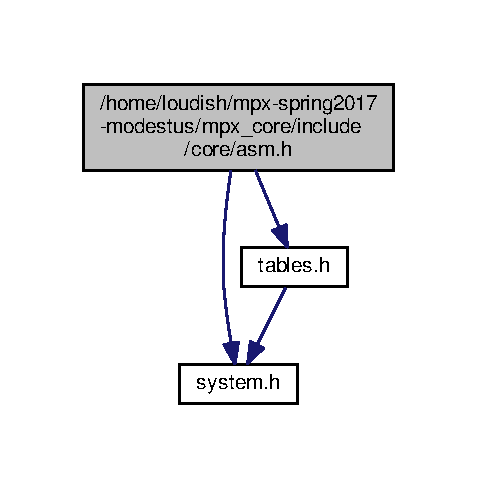
\includegraphics[width=229pt]{asm_8h__incl}
\end{center}
\end{figure}

\hypertarget{commhand_8h}{}\section{/home/loudish/mpx-\/spring2017-\/modestus/mpx\+\_\+core/include/core/commhand.h File Reference}
\label{commhand_8h}\index{/home/loudish/mpx-\/spring2017-\/modestus/mpx\+\_\+core/include/core/commhand.\+h@{/home/loudish/mpx-\/spring2017-\/modestus/mpx\+\_\+core/include/core/commhand.\+h}}
This graph shows which files directly or indirectly include this file\+:\nopagebreak
\begin{figure}[H]
\begin{center}
\leavevmode
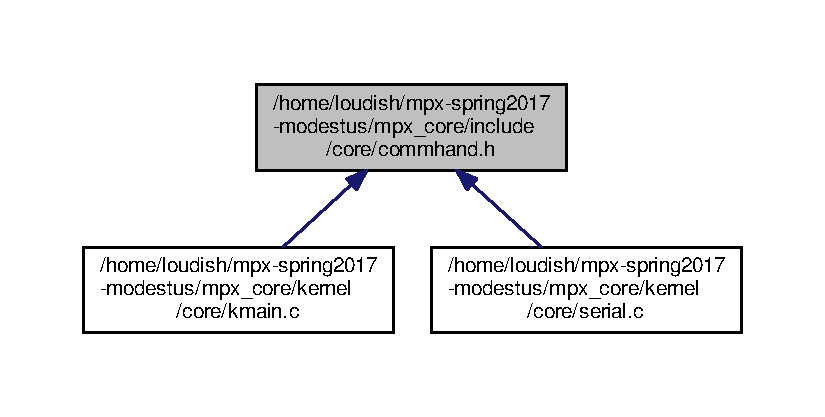
\includegraphics[width=350pt]{commhand_8h__dep__incl}
\end{center}
\end{figure}
\subsection*{Functions}
\begin{DoxyCompactItemize}
\item 
void \hyperlink{commhand_8h_a5f6c259a5d805f1a24d35f36cb9207d3}{init\+\_\+commhand} (void)
\begin{DoxyCompactList}\small\item\em init\+\_\+commhand Starts input loop and waits for shutdown code \end{DoxyCompactList}\item 
char $\ast$ \hyperlink{commhand_8h_a5788474718b834e6c093a1223044c610}{get\+\_\+hist\+\_\+up} (void)
\end{DoxyCompactItemize}


\subsection{Function Documentation}
\index{commhand.\+h@{commhand.\+h}!get\+\_\+hist\+\_\+up@{get\+\_\+hist\+\_\+up}}
\index{get\+\_\+hist\+\_\+up@{get\+\_\+hist\+\_\+up}!commhand.\+h@{commhand.\+h}}
\subsubsection[{\texorpdfstring{get\+\_\+hist\+\_\+up(void)}{get_hist_up(void)}}]{\setlength{\rightskip}{0pt plus 5cm}char$\ast$ get\+\_\+hist\+\_\+up (
\begin{DoxyParamCaption}
\item[{void}]{}
\end{DoxyParamCaption}
)}\hypertarget{commhand_8h_a5788474718b834e6c093a1223044c610}{}\label{commhand_8h_a5788474718b834e6c093a1223044c610}


Definition at line 162 of file commhand.\+c.



References comm\+\_\+hist, and hist\+\_\+i.


\begin{DoxyCode}
162                     \{
163     \hyperlink{commhand_8c_addd367ad6cf3ffe96855b76b451d02d5}{hist\_i}--;
164     \textcolor{keywordflow}{return} \hyperlink{commhand_8c_a3d3b206df340b640d0fca3a5c7436dfe}{comm\_hist}[\hyperlink{commhand_8c_addd367ad6cf3ffe96855b76b451d02d5}{hist\_i}];
165 \}
\end{DoxyCode}
\index{commhand.\+h@{commhand.\+h}!init\+\_\+commhand@{init\+\_\+commhand}}
\index{init\+\_\+commhand@{init\+\_\+commhand}!commhand.\+h@{commhand.\+h}}
\subsubsection[{\texorpdfstring{init\+\_\+commhand(void)}{init_commhand(void)}}]{\setlength{\rightskip}{0pt plus 5cm}void init\+\_\+commhand (
\begin{DoxyParamCaption}
\item[{void}]{}
\end{DoxyParamCaption}
)}\hypertarget{commhand_8h_a5f6c259a5d805f1a24d35f36cb9207d3}{}\label{commhand_8h_a5f6c259a5d805f1a24d35f36cb9207d3}


init\+\_\+commhand Starts input loop and waits for shutdown code 



Definition at line 193 of file commhand.\+c.



References cmd\+Array, exec\+\_\+comm(), in\+\_\+string, init\+Cmd\+Array(), M\+A\+X\+\_\+\+L\+E\+N\+G\+TH, P\+R\+O\+M\+PT, serial\+\_\+poll(), serial\+\_\+print(), shutdown, and strcpy().



Referenced by kmain().


\begin{DoxyCode}
193                          \{
194     \hyperlink{commhand_8c_a95b7dfd9ea5945e05a5e443355de389e}{initCmdArray}(\hyperlink{commhand_8c_a5582c68677f88e6cacb6b1a2086f34c1}{cmdArray});
195 
196     \textcolor{keywordflow}{while}(!\hyperlink{commhand_8c_a5161d377a61befc3f8103e794d5cb582}{shutdown}) \{
197         \hyperlink{serial_8h_a995827efcd4dcfb780c9fbb9645410a4}{serial\_print}(\hyperlink{input_8h_accdbea14ea06c15e271784368bd993e8}{PROMPT});
198         \textcolor{keywordtype}{char} \hyperlink{commhand_8c_a304f731e770f19e932c39d189c8cb56f}{in\_string}[\hyperlink{input_8h_a7a9a231e30b47bc0345749c8bd1e5077}{MAX\_LENGTH}];
199         \hyperlink{string_8h_a1eb9cae61e6a6282c28dbc298ef7297e}{strcpy}(in\_string, \hyperlink{serial_8h_a4b7cdfe478986c0d41a54f2c4a683136}{serial\_poll}(in\_string));
200         \hyperlink{commhand_8c_aeac60d828269ea566f8d5481017467ba}{exec\_comm}(in\_string);
201     \}
202 \}
\end{DoxyCode}

\hypertarget{interrupts_8h}{}\section{/home/loudish/mpx-\/spring2017-\/modestus/mpx\+\_\+core/include/core/interrupts.h File Reference}
\label{interrupts_8h}\index{/home/loudish/mpx-\/spring2017-\/modestus/mpx\+\_\+core/include/core/interrupts.\+h@{/home/loudish/mpx-\/spring2017-\/modestus/mpx\+\_\+core/include/core/interrupts.\+h}}
This graph shows which files directly or indirectly include this file\+:\nopagebreak
\begin{figure}[H]
\begin{center}
\leavevmode
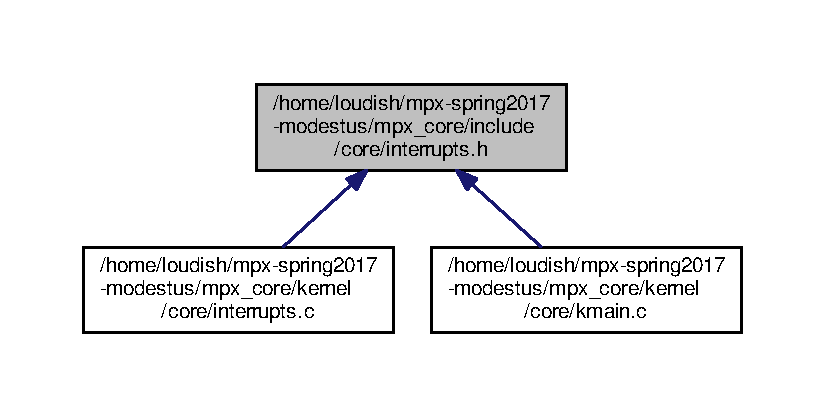
\includegraphics[width=350pt]{interrupts_8h__dep__incl}
\end{center}
\end{figure}
\subsection*{Functions}
\begin{DoxyCompactItemize}
\item 
void \hyperlink{interrupts_8h_ad17d9a8aa78440af8fc40d3fd55dbad8}{init\+\_\+irq} (void)
\item 
void \hyperlink{interrupts_8h_afbc0dbef6f15e2df21b38724ea38c483}{init\+\_\+pic} (void)
\end{DoxyCompactItemize}


\subsection{Function Documentation}
\index{interrupts.\+h@{interrupts.\+h}!init\+\_\+irq@{init\+\_\+irq}}
\index{init\+\_\+irq@{init\+\_\+irq}!interrupts.\+h@{interrupts.\+h}}
\subsubsection[{\texorpdfstring{init\+\_\+irq(void)}{init_irq(void)}}]{\setlength{\rightskip}{0pt plus 5cm}void init\+\_\+irq (
\begin{DoxyParamCaption}
\item[{void}]{}
\end{DoxyParamCaption}
)}\hypertarget{interrupts_8h_ad17d9a8aa78440af8fc40d3fd55dbad8}{}\label{interrupts_8h_ad17d9a8aa78440af8fc40d3fd55dbad8}


Definition at line 66 of file interrupts.\+c.



References bounds(), breakpoint(), coprocessor(), coprocessor\+\_\+segment(), debug(), device\+\_\+not\+\_\+available(), divide\+\_\+error(), double\+\_\+fault(), general\+\_\+protection(), idt\+\_\+set\+\_\+gate(), invalid\+\_\+op(), invalid\+\_\+tss(), nmi(), overflow(), page\+\_\+fault(), reserved(), rtc\+\_\+isr(), segment\+\_\+not\+\_\+present(), and stack\+\_\+segment().



Referenced by kmain().


\begin{DoxyCode}
67 \{  
68   \textcolor{keywordtype}{int} i;
69 
70   \textcolor{comment}{// Necessary interrupt handlers for protected mode}
71   \hyperlink{system_8h_a757de76cafbcddaac0d1632902fe4cb8}{u32int} isrs[17] = \{
72     (\hyperlink{system_8h_a757de76cafbcddaac0d1632902fe4cb8}{u32int})\hyperlink{interrupts_8c_a779cbe32e1a5f1dc8fa9b7191f116b28}{divide\_error},
73     (\hyperlink{system_8h_a757de76cafbcddaac0d1632902fe4cb8}{u32int})\hyperlink{interrupts_8c_a0d0105433f9c65c14928027b3f0966b7}{debug},
74     (\hyperlink{system_8h_a757de76cafbcddaac0d1632902fe4cb8}{u32int})\hyperlink{interrupts_8c_aa42d18df06cf68f8c05fded5344c4c7e}{nmi},
75     (\hyperlink{system_8h_a757de76cafbcddaac0d1632902fe4cb8}{u32int})\hyperlink{interrupts_8c_a874043e2396dd8ce20ec7af3ea1e2a86}{breakpoint},
76     (\hyperlink{system_8h_a757de76cafbcddaac0d1632902fe4cb8}{u32int})\hyperlink{interrupts_8c_a810f078a27a6781a7406c74985ecb761}{overflow},
77     (\hyperlink{system_8h_a757de76cafbcddaac0d1632902fe4cb8}{u32int})\hyperlink{interrupts_8c_a96724d36ad85f9a02231d8e6fe0434df}{bounds},
78     (\hyperlink{system_8h_a757de76cafbcddaac0d1632902fe4cb8}{u32int})\hyperlink{interrupts_8c_a422d8af60b69cc11dbcbb9d89c69756b}{invalid\_op},
79     (\hyperlink{system_8h_a757de76cafbcddaac0d1632902fe4cb8}{u32int})\hyperlink{interrupts_8c_abe88cd1dcc26cb58ee785c714e016f72}{device\_not\_available},
80     (\hyperlink{system_8h_a757de76cafbcddaac0d1632902fe4cb8}{u32int})\hyperlink{interrupts_8c_ae2b9f5b44e05e0c53f8eaaa98396d627}{double\_fault},
81     (\hyperlink{system_8h_a757de76cafbcddaac0d1632902fe4cb8}{u32int})\hyperlink{interrupts_8c_a1d688a0a370977c03fa98884a6e771e9}{coprocessor\_segment},
82     (\hyperlink{system_8h_a757de76cafbcddaac0d1632902fe4cb8}{u32int})\hyperlink{interrupts_8c_a972be67f6a5432cc8eab8d27755fb00f}{invalid\_tss},
83     (\hyperlink{system_8h_a757de76cafbcddaac0d1632902fe4cb8}{u32int})\hyperlink{interrupts_8c_af1748d9ea65ba652bc92074ab6570d8e}{segment\_not\_present},
84     (\hyperlink{system_8h_a757de76cafbcddaac0d1632902fe4cb8}{u32int})\hyperlink{interrupts_8c_a1ccc3198890318741629a03bb88bee6f}{stack\_segment},
85     (\hyperlink{system_8h_a757de76cafbcddaac0d1632902fe4cb8}{u32int})\hyperlink{interrupts_8c_a10777dd6c3a040471676741bbb8dda46}{general\_protection},
86     (\hyperlink{system_8h_a757de76cafbcddaac0d1632902fe4cb8}{u32int})\hyperlink{interrupts_8c_ab3800dd0177baaef4da00494edfb32d9}{page\_fault},
87     (\hyperlink{system_8h_a757de76cafbcddaac0d1632902fe4cb8}{u32int})\hyperlink{interrupts_8c_ad686e3fee8ec8346a6d8e98d970a02dd}{reserved},
88     (\hyperlink{system_8h_a757de76cafbcddaac0d1632902fe4cb8}{u32int})\hyperlink{interrupts_8c_a5c538c7b7a55e3c981780b599fcb1de7}{coprocessor}
89   \};
90 
91   \textcolor{comment}{// Install handlers; 0x08=sel, 0x8e=flags}
92   for(i=0; i<32; i++)\{
93     \textcolor{keywordflow}{if} (i<17) \hyperlink{tables_8h_a9eca3fe1465f8d7d383551d804853139}{idt\_set\_gate}(i, isrs[i], 0x08, 0x8e);
94     \textcolor{keywordflow}{else} \hyperlink{tables_8h_a9eca3fe1465f8d7d383551d804853139}{idt\_set\_gate}(i, (\hyperlink{system_8h_a757de76cafbcddaac0d1632902fe4cb8}{u32int})reserved, 0x08, 0x8e);
95   \}
96   \textcolor{comment}{// Ignore interrupts from the real time clock}
97   \hyperlink{tables_8h_a9eca3fe1465f8d7d383551d804853139}{idt\_set\_gate}(0x08, (\hyperlink{system_8h_a757de76cafbcddaac0d1632902fe4cb8}{u32int})\hyperlink{interrupts_8c_a52f2615cebbdeab188085a03c913fcf9}{rtc\_isr}, 0x08, 0x8e);
98 \}
\end{DoxyCode}
\index{interrupts.\+h@{interrupts.\+h}!init\+\_\+pic@{init\+\_\+pic}}
\index{init\+\_\+pic@{init\+\_\+pic}!interrupts.\+h@{interrupts.\+h}}
\subsubsection[{\texorpdfstring{init\+\_\+pic(void)}{init_pic(void)}}]{\setlength{\rightskip}{0pt plus 5cm}void init\+\_\+pic (
\begin{DoxyParamCaption}
\item[{void}]{}
\end{DoxyParamCaption}
)}\hypertarget{interrupts_8h_afbc0dbef6f15e2df21b38724ea38c483}{}\label{interrupts_8h_afbc0dbef6f15e2df21b38724ea38c483}


Definition at line 106 of file interrupts.\+c.



References I\+C\+W1, I\+C\+W4, io\+\_\+wait, outb, P\+I\+C1, and P\+I\+C2.



Referenced by kmain().


\begin{DoxyCode}
107 \{
108   \hyperlink{io_8h_a0e661d36f40638a36550a534076f155b}{outb}(\hyperlink{interrupts_8c_a6b115109e4a0d3c5fb6252d091e86bfe}{PIC1},\hyperlink{interrupts_8c_ac56445256ce58f14f3c61af0cbf0cdad}{ICW1});   \textcolor{comment}{//send initialization code words 1 to PIC1}
109   \hyperlink{interrupts_8c_aeae4190ed25d0648577e1c742fd8a78d}{io\_wait}();
110   \hyperlink{io_8h_a0e661d36f40638a36550a534076f155b}{outb}(\hyperlink{interrupts_8c_ac90003f52c8d736193efc954ece08e58}{PIC2},\hyperlink{interrupts_8c_ac56445256ce58f14f3c61af0cbf0cdad}{ICW1});   \textcolor{comment}{//send icw1 to PIC2}
111   \hyperlink{interrupts_8c_aeae4190ed25d0648577e1c742fd8a78d}{io\_wait}();
112   \hyperlink{io_8h_a0e661d36f40638a36550a534076f155b}{outb}(\hyperlink{interrupts_8c_a6b115109e4a0d3c5fb6252d091e86bfe}{PIC1}+1,0x20); \textcolor{comment}{//icw2: remap irq0 to 32}
113   \hyperlink{interrupts_8c_aeae4190ed25d0648577e1c742fd8a78d}{io\_wait}();
114   \hyperlink{io_8h_a0e661d36f40638a36550a534076f155b}{outb}(\hyperlink{interrupts_8c_ac90003f52c8d736193efc954ece08e58}{PIC2}+1,0x28); \textcolor{comment}{//icw2: remap irq8 to 40}
115   \hyperlink{interrupts_8c_aeae4190ed25d0648577e1c742fd8a78d}{io\_wait}();
116   \hyperlink{io_8h_a0e661d36f40638a36550a534076f155b}{outb}(\hyperlink{interrupts_8c_a6b115109e4a0d3c5fb6252d091e86bfe}{PIC1}+1,4);    \textcolor{comment}{//icw3}
117   \hyperlink{interrupts_8c_aeae4190ed25d0648577e1c742fd8a78d}{io\_wait}();
118   \hyperlink{io_8h_a0e661d36f40638a36550a534076f155b}{outb}(\hyperlink{interrupts_8c_ac90003f52c8d736193efc954ece08e58}{PIC2}+1,2);    \textcolor{comment}{//icw3}
119   \hyperlink{interrupts_8c_aeae4190ed25d0648577e1c742fd8a78d}{io\_wait}();
120   \hyperlink{io_8h_a0e661d36f40638a36550a534076f155b}{outb}(\hyperlink{interrupts_8c_a6b115109e4a0d3c5fb6252d091e86bfe}{PIC1}+1,\hyperlink{interrupts_8c_a7945f331ddf94a0e0e938f825bc4d43c}{ICW4}); \textcolor{comment}{//icw4: 80x86, automatic handling}
121   \hyperlink{interrupts_8c_aeae4190ed25d0648577e1c742fd8a78d}{io\_wait}();
122   \hyperlink{io_8h_a0e661d36f40638a36550a534076f155b}{outb}(\hyperlink{interrupts_8c_ac90003f52c8d736193efc954ece08e58}{PIC2}+1,\hyperlink{interrupts_8c_a7945f331ddf94a0e0e938f825bc4d43c}{ICW4}); \textcolor{comment}{//icw4: 80x86, automatic handling}
123   \hyperlink{interrupts_8c_aeae4190ed25d0648577e1c742fd8a78d}{io\_wait}();
124   \hyperlink{io_8h_a0e661d36f40638a36550a534076f155b}{outb}(\hyperlink{interrupts_8c_a6b115109e4a0d3c5fb6252d091e86bfe}{PIC1}+1,0xFF); \textcolor{comment}{//disable irqs for PIC1}
125   \hyperlink{interrupts_8c_aeae4190ed25d0648577e1c742fd8a78d}{io\_wait}();
126   \hyperlink{io_8h_a0e661d36f40638a36550a534076f155b}{outb}(\hyperlink{interrupts_8c_ac90003f52c8d736193efc954ece08e58}{PIC2}+1,0xFF); \textcolor{comment}{//disable irqs for PIC2}
127 \}
\end{DoxyCode}

\hypertarget{io_8h}{}\section{/home/loudish/mpx-\/spring2017-\/modestus/mpx\+\_\+core/include/core/io.h File Reference}
\label{io_8h}\index{/home/loudish/mpx-\/spring2017-\/modestus/mpx\+\_\+core/include/core/io.\+h@{/home/loudish/mpx-\/spring2017-\/modestus/mpx\+\_\+core/include/core/io.\+h}}
This graph shows which files directly or indirectly include this file\+:\nopagebreak
\begin{figure}[H]
\begin{center}
\leavevmode
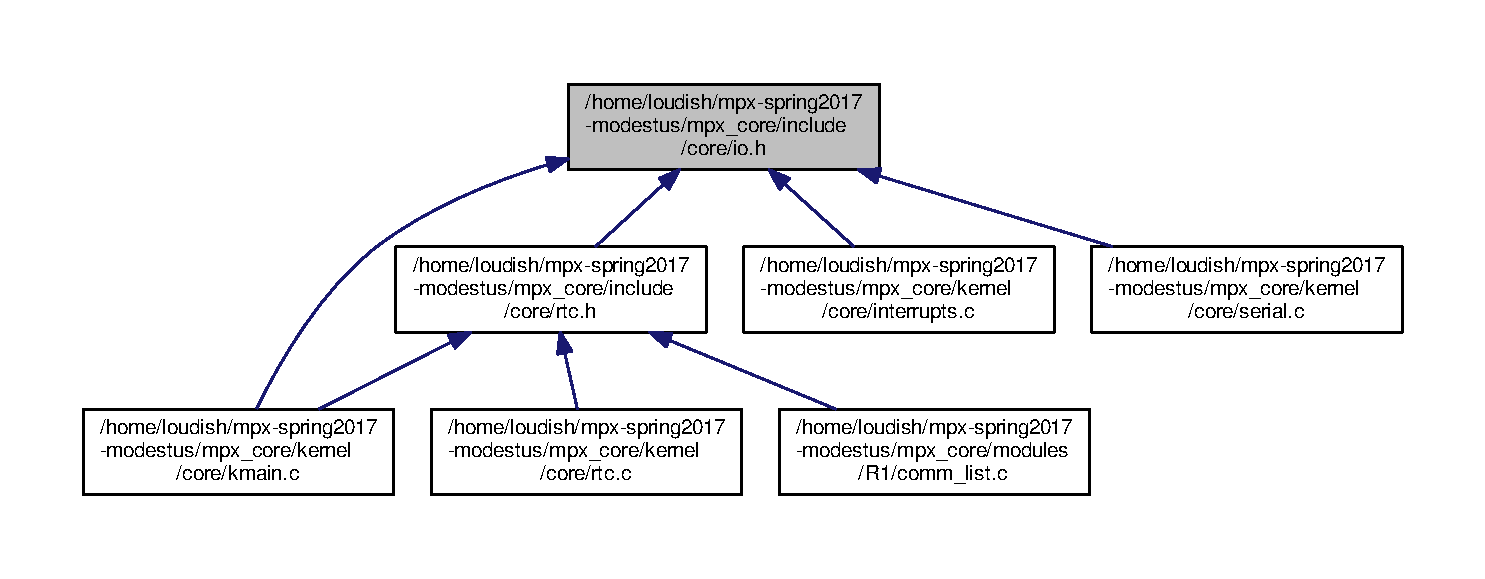
\includegraphics[width=350pt]{io_8h__dep__incl}
\end{center}
\end{figure}
\subsection*{Macros}
\begin{DoxyCompactItemize}
\item 
\#define \hyperlink{io_8h_a0e661d36f40638a36550a534076f155b}{outb}(port,  data)~\hyperlink{system_8h_a71921cebf4610b0dbb2b7a0daaf3fedf}{asm} \hyperlink{system_8h_af55a5e48555be7d32ad73e76cf5d4db0}{volatile} (\char`\"{}outb \%\%al,\%\%dx\char`\"{} \+: \+: \char`\"{}a\char`\"{} (data), \char`\"{}d\char`\"{} (port))
\item 
\#define \hyperlink{io_8h_ad6488a48837d179b1833e2f48dac9665}{inb}(port)
\end{DoxyCompactItemize}


\subsection{Macro Definition Documentation}
\index{io.\+h@{io.\+h}!inb@{inb}}
\index{inb@{inb}!io.\+h@{io.\+h}}
\subsubsection[{\texorpdfstring{inb}{inb}}]{\setlength{\rightskip}{0pt plus 5cm}\#define inb(
\begin{DoxyParamCaption}
\item[{}]{port}
\end{DoxyParamCaption}
)}\hypertarget{io_8h_ad6488a48837d179b1833e2f48dac9665}{}\label{io_8h_ad6488a48837d179b1833e2f48dac9665}
{\bfseries Value\+:}
\begin{DoxyCode}
(\{                      \(\backslash\)
      unsigned \textcolor{keywordtype}{char} r;                      \hyperlink{system_8h_a71921cebf4610b0dbb2b7a0daaf3fedf}{\(\backslash\)}
\hyperlink{system_8h_a71921cebf4610b0dbb2b7a0daaf3fedf}{      asm} \textcolor{keyword}{volatile} (\textcolor{stringliteral}{"inb %%dx,%%al"}: \textcolor{stringliteral}{"=a"} (r): \textcolor{stringliteral}{"d"} (port));    \(\backslash\)
      r;                            \(\backslash\)
    \})
\end{DoxyCode}


Definition at line 15 of file io.\+h.



Referenced by do\+\_\+isr(), get\+\_\+date(), get\+\_\+time(), init\+\_\+serial(), and serial\+\_\+poll().

\index{io.\+h@{io.\+h}!outb@{outb}}
\index{outb@{outb}!io.\+h@{io.\+h}}
\subsubsection[{\texorpdfstring{outb}{outb}}]{\setlength{\rightskip}{0pt plus 5cm}\#define outb(
\begin{DoxyParamCaption}
\item[{}]{port, }
\item[{}]{data}
\end{DoxyParamCaption}
)~{\bf asm} {\bf volatile} (\char`\"{}outb \%\%al,\%\%dx\char`\"{} \+: \+: \char`\"{}a\char`\"{} (data), \char`\"{}d\char`\"{} (port))}\hypertarget{io_8h_a0e661d36f40638a36550a534076f155b}{}\label{io_8h_a0e661d36f40638a36550a534076f155b}


Definition at line 8 of file io.\+h.



Referenced by do\+\_\+isr(), get\+\_\+date(), get\+\_\+time(), init\+\_\+pic(), init\+\_\+serial(), serial\+\_\+print(), serial\+\_\+println(), set\+\_\+date(), and set\+\_\+time().


\hypertarget{include_2core_2mpx__supt_8h}{}\section{/home/loudish/mpx-\/spring2017-\/modestus/mpx\+\_\+core/include/core/mpx\+\_\+supt.h File Reference}
\label{include_2core_2mpx__supt_8h}\index{/home/loudish/mpx-\/spring2017-\/modestus/mpx\+\_\+core/include/core/mpx\+\_\+supt.\+h@{/home/loudish/mpx-\/spring2017-\/modestus/mpx\+\_\+core/include/core/mpx\+\_\+supt.\+h}}
{\ttfamily \#include $<$system.\+h$>$}\\*
Include dependency graph for mpx\+\_\+supt.\+h\+:\nopagebreak
\begin{figure}[H]
\begin{center}
\leavevmode
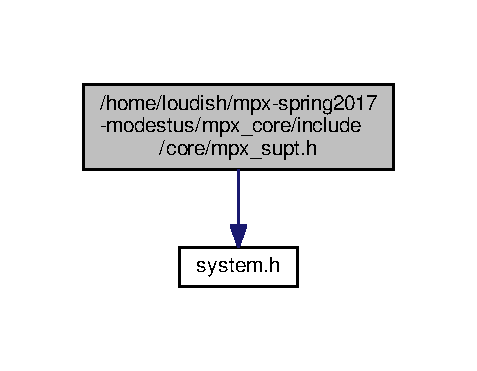
\includegraphics[width=229pt]{include_2core_2mpx__supt_8h__incl}
\end{center}
\end{figure}
This graph shows which files directly or indirectly include this file\+:\nopagebreak
\begin{figure}[H]
\begin{center}
\leavevmode
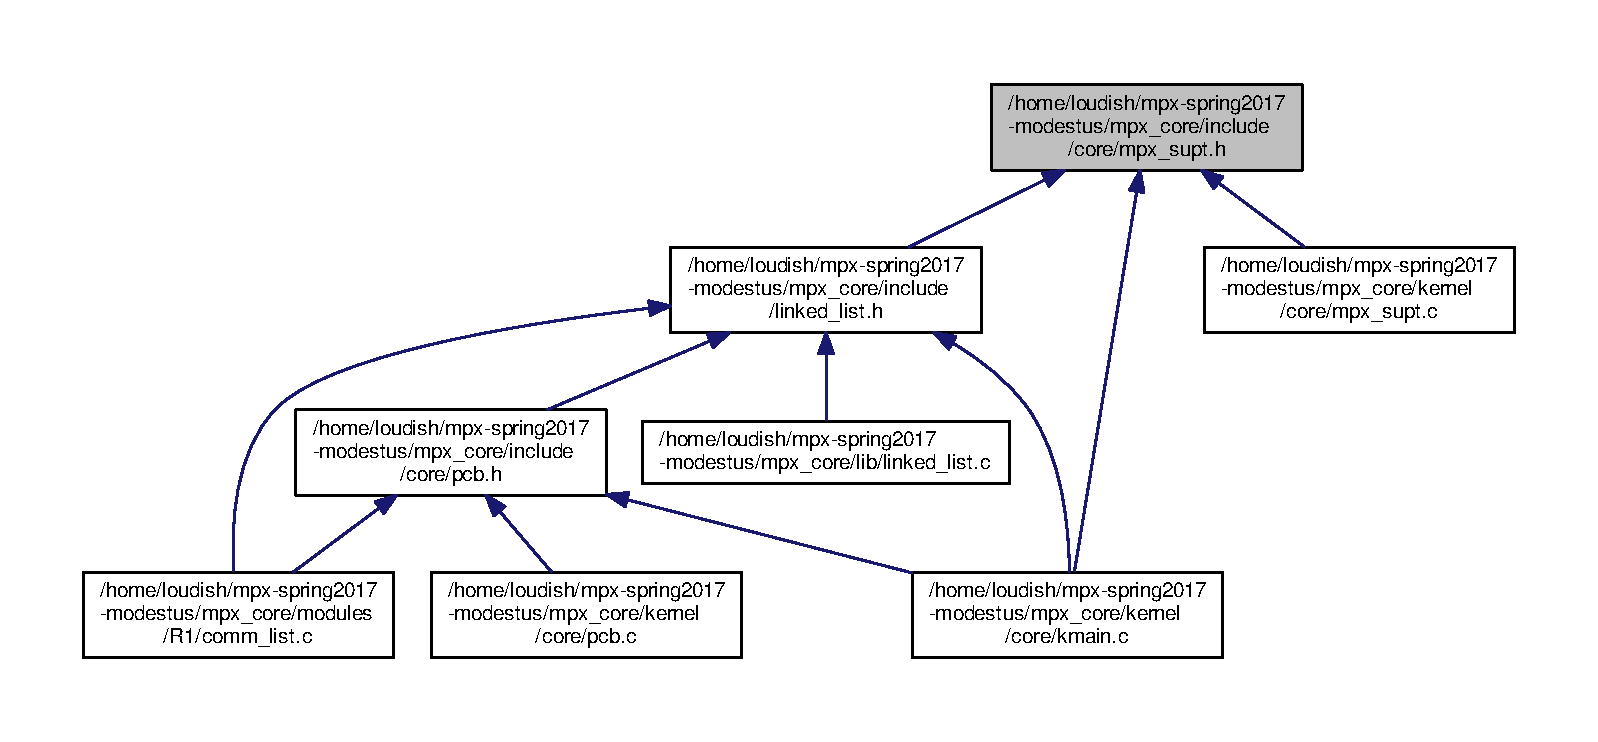
\includegraphics[width=350pt]{include_2core_2mpx__supt_8h__dep__incl}
\end{center}
\end{figure}
\subsection*{Data Structures}
\begin{DoxyCompactItemize}
\item 
struct \hyperlink{structparam}{param}
\end{DoxyCompactItemize}
\subsection*{Macros}
\begin{DoxyCompactItemize}
\item 
\#define \hyperlink{include_2core_2mpx__supt_8h_ad111e603bbebe5d87f6bc39264ce4733}{E\+X\+IT}~0
\item 
\#define \hyperlink{include_2core_2mpx__supt_8h_a9c21a7caee326d7803b94ae1952b27ca}{I\+D\+LE}~1
\item 
\#define \hyperlink{include_2core_2mpx__supt_8h_ada74e7db007a68e763f20c17f2985356}{R\+E\+AD}~2
\item 
\#define \hyperlink{include_2core_2mpx__supt_8h_aa10f470e996d0f51210d24f442d25e1e}{W\+R\+I\+TE}~3
\item 
\#define \hyperlink{include_2core_2mpx__supt_8h_a9d88621bfb79cb860b9ea2b5abb1c7f0}{M\+O\+D\+U\+L\+E\+\_\+\+R1}~0
\item 
\#define \hyperlink{include_2core_2mpx__supt_8h_a177f46669733cd706e9476485dfd961b}{M\+O\+D\+U\+L\+E\+\_\+\+R2}~1
\item 
\#define \hyperlink{include_2core_2mpx__supt_8h_afe0ac8d1ebddd519bed41c8d8e79fad0}{M\+O\+D\+U\+L\+E\+\_\+\+R3}~2
\item 
\#define \hyperlink{include_2core_2mpx__supt_8h_a05541487bcf6e840b918f0a6ef097024}{M\+O\+D\+U\+L\+E\+\_\+\+R4}~4
\item 
\#define \hyperlink{include_2core_2mpx__supt_8h_a68745bb3b58fd02dcee2cad3b2331def}{M\+O\+D\+U\+L\+E\+\_\+\+R5}~8
\end{DoxyCompactItemize}
\subsection*{Functions}
\begin{DoxyCompactItemize}
\item 
int \hyperlink{include_2core_2mpx__supt_8h_afb6ff5e2e9bdde9d8971a497b6fe38ae}{sys\+\_\+req} (int op\+\_\+code)
\item 
void \hyperlink{include_2core_2mpx__supt_8h_a53332c6a3107a4feed6e2e79690a6ffa}{mpx\+\_\+init} (int cur\+\_\+mod)
\item 
void \hyperlink{include_2core_2mpx__supt_8h_a4a28bb188c9fed51228c46980b20e605}{sys\+\_\+set\+\_\+malloc} (\hyperlink{system_8h_a757de76cafbcddaac0d1632902fe4cb8}{u32int}($\ast$func)(\hyperlink{system_8h_a757de76cafbcddaac0d1632902fe4cb8}{u32int}))
\item 
void \hyperlink{include_2core_2mpx__supt_8h_a2463d934fa39601c275a3ade8afd18bc}{sys\+\_\+set\+\_\+free} (int($\ast$func)(void $\ast$))
\item 
void $\ast$ \hyperlink{include_2core_2mpx__supt_8h_a61adad2abba0a3a225c2290b3de1fe93}{sys\+\_\+alloc\+\_\+mem} (\hyperlink{system_8h_a757de76cafbcddaac0d1632902fe4cb8}{u32int} size)
\item 
int \hyperlink{include_2core_2mpx__supt_8h_a950663d39dbb073c9dff9cf3b5d3392c}{sys\+\_\+free\+\_\+mem} (void $\ast$ptr)
\item 
void \hyperlink{include_2core_2mpx__supt_8h_a83abbeda22fc5e6c2b35523b64199c1c}{idle} ()
\end{DoxyCompactItemize}


\subsection{Macro Definition Documentation}
\index{include/core/mpx\+\_\+supt.\+h@{include/core/mpx\+\_\+supt.\+h}!E\+X\+IT@{E\+X\+IT}}
\index{E\+X\+IT@{E\+X\+IT}!include/core/mpx\+\_\+supt.\+h@{include/core/mpx\+\_\+supt.\+h}}
\subsubsection[{\texorpdfstring{E\+X\+IT}{EXIT}}]{\setlength{\rightskip}{0pt plus 5cm}\#define E\+X\+IT~0}\hypertarget{include_2core_2mpx__supt_8h_ad111e603bbebe5d87f6bc39264ce4733}{}\label{include_2core_2mpx__supt_8h_ad111e603bbebe5d87f6bc39264ce4733}


Definition at line 6 of file mpx\+\_\+supt.\+h.

\index{include/core/mpx\+\_\+supt.\+h@{include/core/mpx\+\_\+supt.\+h}!I\+D\+LE@{I\+D\+LE}}
\index{I\+D\+LE@{I\+D\+LE}!include/core/mpx\+\_\+supt.\+h@{include/core/mpx\+\_\+supt.\+h}}
\subsubsection[{\texorpdfstring{I\+D\+LE}{IDLE}}]{\setlength{\rightskip}{0pt plus 5cm}\#define I\+D\+LE~1}\hypertarget{include_2core_2mpx__supt_8h_a9c21a7caee326d7803b94ae1952b27ca}{}\label{include_2core_2mpx__supt_8h_a9c21a7caee326d7803b94ae1952b27ca}


Definition at line 7 of file mpx\+\_\+supt.\+h.



Referenced by idle().

\index{include/core/mpx\+\_\+supt.\+h@{include/core/mpx\+\_\+supt.\+h}!M\+O\+D\+U\+L\+E\+\_\+\+R1@{M\+O\+D\+U\+L\+E\+\_\+\+R1}}
\index{M\+O\+D\+U\+L\+E\+\_\+\+R1@{M\+O\+D\+U\+L\+E\+\_\+\+R1}!include/core/mpx\+\_\+supt.\+h@{include/core/mpx\+\_\+supt.\+h}}
\subsubsection[{\texorpdfstring{M\+O\+D\+U\+L\+E\+\_\+\+R1}{MODULE_R1}}]{\setlength{\rightskip}{0pt plus 5cm}\#define M\+O\+D\+U\+L\+E\+\_\+\+R1~0}\hypertarget{include_2core_2mpx__supt_8h_a9d88621bfb79cb860b9ea2b5abb1c7f0}{}\label{include_2core_2mpx__supt_8h_a9d88621bfb79cb860b9ea2b5abb1c7f0}


Definition at line 11 of file mpx\+\_\+supt.\+h.

\index{include/core/mpx\+\_\+supt.\+h@{include/core/mpx\+\_\+supt.\+h}!M\+O\+D\+U\+L\+E\+\_\+\+R2@{M\+O\+D\+U\+L\+E\+\_\+\+R2}}
\index{M\+O\+D\+U\+L\+E\+\_\+\+R2@{M\+O\+D\+U\+L\+E\+\_\+\+R2}!include/core/mpx\+\_\+supt.\+h@{include/core/mpx\+\_\+supt.\+h}}
\subsubsection[{\texorpdfstring{M\+O\+D\+U\+L\+E\+\_\+\+R2}{MODULE_R2}}]{\setlength{\rightskip}{0pt plus 5cm}\#define M\+O\+D\+U\+L\+E\+\_\+\+R2~1}\hypertarget{include_2core_2mpx__supt_8h_a177f46669733cd706e9476485dfd961b}{}\label{include_2core_2mpx__supt_8h_a177f46669733cd706e9476485dfd961b}


Definition at line 12 of file mpx\+\_\+supt.\+h.

\index{include/core/mpx\+\_\+supt.\+h@{include/core/mpx\+\_\+supt.\+h}!M\+O\+D\+U\+L\+E\+\_\+\+R3@{M\+O\+D\+U\+L\+E\+\_\+\+R3}}
\index{M\+O\+D\+U\+L\+E\+\_\+\+R3@{M\+O\+D\+U\+L\+E\+\_\+\+R3}!include/core/mpx\+\_\+supt.\+h@{include/core/mpx\+\_\+supt.\+h}}
\subsubsection[{\texorpdfstring{M\+O\+D\+U\+L\+E\+\_\+\+R3}{MODULE_R3}}]{\setlength{\rightskip}{0pt plus 5cm}\#define M\+O\+D\+U\+L\+E\+\_\+\+R3~2}\hypertarget{include_2core_2mpx__supt_8h_afe0ac8d1ebddd519bed41c8d8e79fad0}{}\label{include_2core_2mpx__supt_8h_afe0ac8d1ebddd519bed41c8d8e79fad0}


Definition at line 13 of file mpx\+\_\+supt.\+h.

\index{include/core/mpx\+\_\+supt.\+h@{include/core/mpx\+\_\+supt.\+h}!M\+O\+D\+U\+L\+E\+\_\+\+R4@{M\+O\+D\+U\+L\+E\+\_\+\+R4}}
\index{M\+O\+D\+U\+L\+E\+\_\+\+R4@{M\+O\+D\+U\+L\+E\+\_\+\+R4}!include/core/mpx\+\_\+supt.\+h@{include/core/mpx\+\_\+supt.\+h}}
\subsubsection[{\texorpdfstring{M\+O\+D\+U\+L\+E\+\_\+\+R4}{MODULE_R4}}]{\setlength{\rightskip}{0pt plus 5cm}\#define M\+O\+D\+U\+L\+E\+\_\+\+R4~4}\hypertarget{include_2core_2mpx__supt_8h_a05541487bcf6e840b918f0a6ef097024}{}\label{include_2core_2mpx__supt_8h_a05541487bcf6e840b918f0a6ef097024}


Definition at line 14 of file mpx\+\_\+supt.\+h.

\index{include/core/mpx\+\_\+supt.\+h@{include/core/mpx\+\_\+supt.\+h}!M\+O\+D\+U\+L\+E\+\_\+\+R5@{M\+O\+D\+U\+L\+E\+\_\+\+R5}}
\index{M\+O\+D\+U\+L\+E\+\_\+\+R5@{M\+O\+D\+U\+L\+E\+\_\+\+R5}!include/core/mpx\+\_\+supt.\+h@{include/core/mpx\+\_\+supt.\+h}}
\subsubsection[{\texorpdfstring{M\+O\+D\+U\+L\+E\+\_\+\+R5}{MODULE_R5}}]{\setlength{\rightskip}{0pt plus 5cm}\#define M\+O\+D\+U\+L\+E\+\_\+\+R5~8}\hypertarget{include_2core_2mpx__supt_8h_a68745bb3b58fd02dcee2cad3b2331def}{}\label{include_2core_2mpx__supt_8h_a68745bb3b58fd02dcee2cad3b2331def}


Definition at line 15 of file mpx\+\_\+supt.\+h.



Referenced by sys\+\_\+alloc\+\_\+mem(), and sys\+\_\+free\+\_\+mem().

\index{include/core/mpx\+\_\+supt.\+h@{include/core/mpx\+\_\+supt.\+h}!R\+E\+AD@{R\+E\+AD}}
\index{R\+E\+AD@{R\+E\+AD}!include/core/mpx\+\_\+supt.\+h@{include/core/mpx\+\_\+supt.\+h}}
\subsubsection[{\texorpdfstring{R\+E\+AD}{READ}}]{\setlength{\rightskip}{0pt plus 5cm}\#define R\+E\+AD~2}\hypertarget{include_2core_2mpx__supt_8h_ada74e7db007a68e763f20c17f2985356}{}\label{include_2core_2mpx__supt_8h_ada74e7db007a68e763f20c17f2985356}


Definition at line 8 of file mpx\+\_\+supt.\+h.

\index{include/core/mpx\+\_\+supt.\+h@{include/core/mpx\+\_\+supt.\+h}!W\+R\+I\+TE@{W\+R\+I\+TE}}
\index{W\+R\+I\+TE@{W\+R\+I\+TE}!include/core/mpx\+\_\+supt.\+h@{include/core/mpx\+\_\+supt.\+h}}
\subsubsection[{\texorpdfstring{W\+R\+I\+TE}{WRITE}}]{\setlength{\rightskip}{0pt plus 5cm}\#define W\+R\+I\+TE~3}\hypertarget{include_2core_2mpx__supt_8h_aa10f470e996d0f51210d24f442d25e1e}{}\label{include_2core_2mpx__supt_8h_aa10f470e996d0f51210d24f442d25e1e}


Definition at line 9 of file mpx\+\_\+supt.\+h.



\subsection{Function Documentation}
\index{include/core/mpx\+\_\+supt.\+h@{include/core/mpx\+\_\+supt.\+h}!idle@{idle}}
\index{idle@{idle}!include/core/mpx\+\_\+supt.\+h@{include/core/mpx\+\_\+supt.\+h}}
\subsubsection[{\texorpdfstring{idle()}{idle()}}]{\setlength{\rightskip}{0pt plus 5cm}void idle (
\begin{DoxyParamCaption}
{}
\end{DoxyParamCaption}
)}\hypertarget{include_2core_2mpx__supt_8h_a83abbeda22fc5e6c2b35523b64199c1c}{}\label{include_2core_2mpx__supt_8h_a83abbeda22fc5e6c2b35523b64199c1c}


Definition at line 47 of file mpx\+\_\+supt.\+c.


\begin{DoxyCode}
48 \{
49   \textcolor{keywordflow}{while}(1)\{
50     \hyperlink{kernel_2core_2mpx__supt_8c_afb6ff5e2e9bdde9d8971a497b6fe38ae}{sys\_req}(\hyperlink{include_2core_2mpx__supt_8h_a9c21a7caee326d7803b94ae1952b27ca}{IDLE});
51   \}
52 \}
\end{DoxyCode}
\index{include/core/mpx\+\_\+supt.\+h@{include/core/mpx\+\_\+supt.\+h}!mpx\+\_\+init@{mpx\+\_\+init}}
\index{mpx\+\_\+init@{mpx\+\_\+init}!include/core/mpx\+\_\+supt.\+h@{include/core/mpx\+\_\+supt.\+h}}
\subsubsection[{\texorpdfstring{mpx\+\_\+init(int cur\+\_\+mod)}{mpx_init(int cur_mod)}}]{\setlength{\rightskip}{0pt plus 5cm}void mpx\+\_\+init (
\begin{DoxyParamCaption}
\item[{int}]{cur\+\_\+mod}
\end{DoxyParamCaption}
)}\hypertarget{include_2core_2mpx__supt_8h_a53332c6a3107a4feed6e2e79690a6ffa}{}\label{include_2core_2mpx__supt_8h_a53332c6a3107a4feed6e2e79690a6ffa}


Definition at line 16 of file mpx\+\_\+supt.\+c.


\begin{DoxyCode}
17 \{
18   \hyperlink{kernel_2core_2mpx__supt_8c_a3d19c725b7f9f45e9da97a79ca6a4737}{current\_module} = cur\_mod;
19 \}
\end{DoxyCode}
\index{include/core/mpx\+\_\+supt.\+h@{include/core/mpx\+\_\+supt.\+h}!sys\+\_\+alloc\+\_\+mem@{sys\+\_\+alloc\+\_\+mem}}
\index{sys\+\_\+alloc\+\_\+mem@{sys\+\_\+alloc\+\_\+mem}!include/core/mpx\+\_\+supt.\+h@{include/core/mpx\+\_\+supt.\+h}}
\subsubsection[{\texorpdfstring{sys\+\_\+alloc\+\_\+mem(u32int size)}{sys_alloc_mem(u32int size)}}]{\setlength{\rightskip}{0pt plus 5cm}void$\ast$ sys\+\_\+alloc\+\_\+mem (
\begin{DoxyParamCaption}
\item[{{\bf u32int}}]{size}
\end{DoxyParamCaption}
)}\hypertarget{include_2core_2mpx__supt_8h_a61adad2abba0a3a225c2290b3de1fe93}{}\label{include_2core_2mpx__supt_8h_a61adad2abba0a3a225c2290b3de1fe93}


Definition at line 31 of file mpx\+\_\+supt.\+c.



Referenced by allocate\+P\+C\+B(), and make\+New\+Node().


\begin{DoxyCode}
32 \{
33   \textcolor{keywordflow}{if} (\hyperlink{kernel_2core_2mpx__supt_8c_a3d19c725b7f9f45e9da97a79ca6a4737}{current\_module} < \hyperlink{include_2core_2mpx__supt_8h_a68745bb3b58fd02dcee2cad3b2331def}{MODULE\_R5})
34     \textcolor{keywordflow}{return} (\textcolor{keywordtype}{void} *) \hyperlink{heap_8h_a15d6a52c5c080c8c7ffc73e336d8e574}{kmalloc}(size);
35   \textcolor{keywordflow}{else}
36     \textcolor{keywordflow}{return} (\textcolor{keywordtype}{void} *) (*student\_malloc)(size);
37 \}
\end{DoxyCode}
\index{include/core/mpx\+\_\+supt.\+h@{include/core/mpx\+\_\+supt.\+h}!sys\+\_\+free\+\_\+mem@{sys\+\_\+free\+\_\+mem}}
\index{sys\+\_\+free\+\_\+mem@{sys\+\_\+free\+\_\+mem}!include/core/mpx\+\_\+supt.\+h@{include/core/mpx\+\_\+supt.\+h}}
\subsubsection[{\texorpdfstring{sys\+\_\+free\+\_\+mem(void $\ast$ptr)}{sys_free_mem(void *ptr)}}]{\setlength{\rightskip}{0pt plus 5cm}int sys\+\_\+free\+\_\+mem (
\begin{DoxyParamCaption}
\item[{void $\ast$}]{ptr}
\end{DoxyParamCaption}
)}\hypertarget{include_2core_2mpx__supt_8h_a950663d39dbb073c9dff9cf3b5d3392c}{}\label{include_2core_2mpx__supt_8h_a950663d39dbb073c9dff9cf3b5d3392c}


Definition at line 39 of file mpx\+\_\+supt.\+c.



Referenced by free\+P\+C\+B().


\begin{DoxyCode}
40 \{
41   \textcolor{keywordflow}{if} (\hyperlink{kernel_2core_2mpx__supt_8c_a3d19c725b7f9f45e9da97a79ca6a4737}{current\_module} >= \hyperlink{include_2core_2mpx__supt_8h_a68745bb3b58fd02dcee2cad3b2331def}{MODULE\_R5})
42     \textcolor{keywordflow}{return} (*\hyperlink{kernel_2core_2mpx__supt_8c_a19c47c02b0338bc13716d98305bb8a34}{student\_free})(ptr);
43   \textcolor{comment}{// otherwise we don't free anything}
44   \textcolor{keywordflow}{return} -1;
45 \}
\end{DoxyCode}
\index{include/core/mpx\+\_\+supt.\+h@{include/core/mpx\+\_\+supt.\+h}!sys\+\_\+req@{sys\+\_\+req}}
\index{sys\+\_\+req@{sys\+\_\+req}!include/core/mpx\+\_\+supt.\+h@{include/core/mpx\+\_\+supt.\+h}}
\subsubsection[{\texorpdfstring{sys\+\_\+req(int op\+\_\+code)}{sys_req(int op_code)}}]{\setlength{\rightskip}{0pt plus 5cm}int sys\+\_\+req (
\begin{DoxyParamCaption}
\item[{int}]{op\+\_\+code}
\end{DoxyParamCaption}
)}\hypertarget{include_2core_2mpx__supt_8h_afb6ff5e2e9bdde9d8971a497b6fe38ae}{}\label{include_2core_2mpx__supt_8h_afb6ff5e2e9bdde9d8971a497b6fe38ae}


Definition at line 9 of file mpx\+\_\+supt.\+c.


\begin{DoxyCode}
10 \{
11   \hyperlink{kernel_2core_2mpx__supt_8c_a3b4b77494d0fad58939896ddc5290c99}{params}.\hyperlink{structparam_a81c8b24055c2908ebe480598aba6044c}{op\_code} = op\_code;
12   \textcolor{keyword}{asm} \textcolor{keyword}{volatile} (\textcolor{stringliteral}{"int $60"});
13   \textcolor{keywordflow}{return} 0;
14 \}
\end{DoxyCode}
\index{include/core/mpx\+\_\+supt.\+h@{include/core/mpx\+\_\+supt.\+h}!sys\+\_\+set\+\_\+free@{sys\+\_\+set\+\_\+free}}
\index{sys\+\_\+set\+\_\+free@{sys\+\_\+set\+\_\+free}!include/core/mpx\+\_\+supt.\+h@{include/core/mpx\+\_\+supt.\+h}}
\subsubsection[{\texorpdfstring{sys\+\_\+set\+\_\+free(int($\ast$func)(void $\ast$))}{sys_set_free(int(*func)(void *))}}]{\setlength{\rightskip}{0pt plus 5cm}void sys\+\_\+set\+\_\+free (
\begin{DoxyParamCaption}
\item[{int($\ast$)(void $\ast$)}]{func}
\end{DoxyParamCaption}
)}\hypertarget{include_2core_2mpx__supt_8h_a2463d934fa39601c275a3ade8afd18bc}{}\label{include_2core_2mpx__supt_8h_a2463d934fa39601c275a3ade8afd18bc}


Definition at line 26 of file mpx\+\_\+supt.\+c.


\begin{DoxyCode}
27 \{
28   \hyperlink{kernel_2core_2mpx__supt_8c_a19c47c02b0338bc13716d98305bb8a34}{student\_free} = func;
29 \}
\end{DoxyCode}
\index{include/core/mpx\+\_\+supt.\+h@{include/core/mpx\+\_\+supt.\+h}!sys\+\_\+set\+\_\+malloc@{sys\+\_\+set\+\_\+malloc}}
\index{sys\+\_\+set\+\_\+malloc@{sys\+\_\+set\+\_\+malloc}!include/core/mpx\+\_\+supt.\+h@{include/core/mpx\+\_\+supt.\+h}}
\subsubsection[{\texorpdfstring{sys\+\_\+set\+\_\+malloc(u32int($\ast$func)(u32int))}{sys_set_malloc(u32int(*func)(u32int))}}]{\setlength{\rightskip}{0pt plus 5cm}void sys\+\_\+set\+\_\+malloc (
\begin{DoxyParamCaption}
\item[{{\bf u32int}($\ast$)({\bf u32int})}]{func}
\end{DoxyParamCaption}
)}\hypertarget{include_2core_2mpx__supt_8h_a4a28bb188c9fed51228c46980b20e605}{}\label{include_2core_2mpx__supt_8h_a4a28bb188c9fed51228c46980b20e605}


Definition at line 21 of file mpx\+\_\+supt.\+c.


\begin{DoxyCode}
22 \{
23   \hyperlink{kernel_2core_2mpx__supt_8c_a421e2b48efb5facc71d16979252710e2}{student\_malloc} = func;
24 \}
\end{DoxyCode}

\hypertarget{modules_2mpx__supt_8h}{}\section{/home/loudish/mpx-\/spring2017-\/modestus/mpx\+\_\+core/modules/mpx\+\_\+supt.h File Reference}
\label{modules_2mpx__supt_8h}\index{/home/loudish/mpx-\/spring2017-\/modestus/mpx\+\_\+core/modules/mpx\+\_\+supt.\+h@{/home/loudish/mpx-\/spring2017-\/modestus/mpx\+\_\+core/modules/mpx\+\_\+supt.\+h}}
{\ttfamily \#include $<$system.\+h$>$}\\*
Include dependency graph for mpx\+\_\+supt.\+h\+:\nopagebreak
\begin{figure}[H]
\begin{center}
\leavevmode
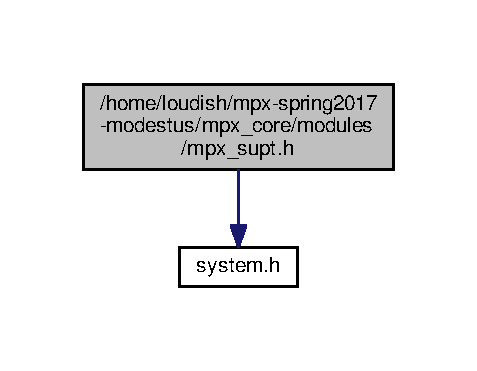
\includegraphics[width=229pt]{modules_2mpx__supt_8h__incl}
\end{center}
\end{figure}
This graph shows which files directly or indirectly include this file\+:\nopagebreak
\begin{figure}[H]
\begin{center}
\leavevmode
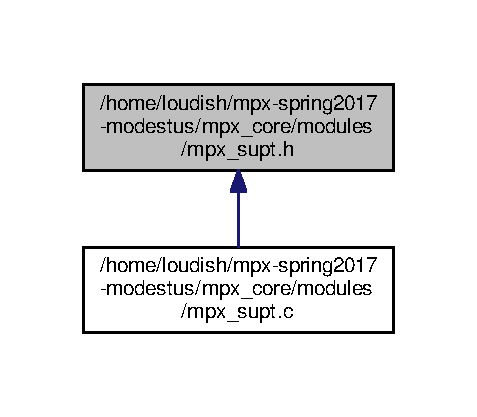
\includegraphics[width=229pt]{modules_2mpx__supt_8h__dep__incl}
\end{center}
\end{figure}
\subsection*{Data Structures}
\begin{DoxyCompactItemize}
\item 
struct \hyperlink{structparam}{param}
\end{DoxyCompactItemize}
\subsection*{Macros}
\begin{DoxyCompactItemize}
\item 
\#define \hyperlink{modules_2mpx__supt_8h_ad111e603bbebe5d87f6bc39264ce4733}{E\+X\+IT}~0
\item 
\#define \hyperlink{modules_2mpx__supt_8h_a9c21a7caee326d7803b94ae1952b27ca}{I\+D\+LE}~1
\item 
\#define \hyperlink{modules_2mpx__supt_8h_ada74e7db007a68e763f20c17f2985356}{R\+E\+AD}~2
\item 
\#define \hyperlink{modules_2mpx__supt_8h_aa10f470e996d0f51210d24f442d25e1e}{W\+R\+I\+TE}~3
\item 
\#define \hyperlink{modules_2mpx__supt_8h_a9d88621bfb79cb860b9ea2b5abb1c7f0}{M\+O\+D\+U\+L\+E\+\_\+\+R1}~0
\item 
\#define \hyperlink{modules_2mpx__supt_8h_a177f46669733cd706e9476485dfd961b}{M\+O\+D\+U\+L\+E\+\_\+\+R2}~1
\item 
\#define \hyperlink{modules_2mpx__supt_8h_afe0ac8d1ebddd519bed41c8d8e79fad0}{M\+O\+D\+U\+L\+E\+\_\+\+R3}~2
\item 
\#define \hyperlink{modules_2mpx__supt_8h_a05541487bcf6e840b918f0a6ef097024}{M\+O\+D\+U\+L\+E\+\_\+\+R4}~4
\item 
\#define \hyperlink{modules_2mpx__supt_8h_a68745bb3b58fd02dcee2cad3b2331def}{M\+O\+D\+U\+L\+E\+\_\+\+R5}~8
\end{DoxyCompactItemize}
\subsection*{Functions}
\begin{DoxyCompactItemize}
\item 
int \hyperlink{modules_2mpx__supt_8h_afb6ff5e2e9bdde9d8971a497b6fe38ae}{sys\+\_\+req} (int op\+\_\+code)
\item 
void \hyperlink{modules_2mpx__supt_8h_a53332c6a3107a4feed6e2e79690a6ffa}{mpx\+\_\+init} (int cur\+\_\+mod)
\item 
void \hyperlink{modules_2mpx__supt_8h_a4a28bb188c9fed51228c46980b20e605}{sys\+\_\+set\+\_\+malloc} (\hyperlink{system_8h_a757de76cafbcddaac0d1632902fe4cb8}{u32int}($\ast$func)(\hyperlink{system_8h_a757de76cafbcddaac0d1632902fe4cb8}{u32int}))
\item 
void \hyperlink{modules_2mpx__supt_8h_a2463d934fa39601c275a3ade8afd18bc}{sys\+\_\+set\+\_\+free} (int($\ast$func)(void $\ast$))
\item 
void $\ast$ \hyperlink{modules_2mpx__supt_8h_a61adad2abba0a3a225c2290b3de1fe93}{sys\+\_\+alloc\+\_\+mem} (\hyperlink{system_8h_a757de76cafbcddaac0d1632902fe4cb8}{u32int} size)
\item 
int \hyperlink{modules_2mpx__supt_8h_a950663d39dbb073c9dff9cf3b5d3392c}{sys\+\_\+free\+\_\+mem} (void $\ast$ptr)
\item 
void \hyperlink{modules_2mpx__supt_8h_a83abbeda22fc5e6c2b35523b64199c1c}{idle} ()
\end{DoxyCompactItemize}


\subsection{Macro Definition Documentation}
\index{modules/mpx\+\_\+supt.\+h@{modules/mpx\+\_\+supt.\+h}!E\+X\+IT@{E\+X\+IT}}
\index{E\+X\+IT@{E\+X\+IT}!modules/mpx\+\_\+supt.\+h@{modules/mpx\+\_\+supt.\+h}}
\subsubsection[{\texorpdfstring{E\+X\+IT}{EXIT}}]{\setlength{\rightskip}{0pt plus 5cm}\#define E\+X\+IT~0}\hypertarget{modules_2mpx__supt_8h_ad111e603bbebe5d87f6bc39264ce4733}{}\label{modules_2mpx__supt_8h_ad111e603bbebe5d87f6bc39264ce4733}


Definition at line 6 of file mpx\+\_\+supt.\+h.

\index{modules/mpx\+\_\+supt.\+h@{modules/mpx\+\_\+supt.\+h}!I\+D\+LE@{I\+D\+LE}}
\index{I\+D\+LE@{I\+D\+LE}!modules/mpx\+\_\+supt.\+h@{modules/mpx\+\_\+supt.\+h}}
\subsubsection[{\texorpdfstring{I\+D\+LE}{IDLE}}]{\setlength{\rightskip}{0pt plus 5cm}\#define I\+D\+LE~1}\hypertarget{modules_2mpx__supt_8h_a9c21a7caee326d7803b94ae1952b27ca}{}\label{modules_2mpx__supt_8h_a9c21a7caee326d7803b94ae1952b27ca}


Definition at line 7 of file mpx\+\_\+supt.\+h.

\index{modules/mpx\+\_\+supt.\+h@{modules/mpx\+\_\+supt.\+h}!M\+O\+D\+U\+L\+E\+\_\+\+R1@{M\+O\+D\+U\+L\+E\+\_\+\+R1}}
\index{M\+O\+D\+U\+L\+E\+\_\+\+R1@{M\+O\+D\+U\+L\+E\+\_\+\+R1}!modules/mpx\+\_\+supt.\+h@{modules/mpx\+\_\+supt.\+h}}
\subsubsection[{\texorpdfstring{M\+O\+D\+U\+L\+E\+\_\+\+R1}{MODULE_R1}}]{\setlength{\rightskip}{0pt plus 5cm}\#define M\+O\+D\+U\+L\+E\+\_\+\+R1~0}\hypertarget{modules_2mpx__supt_8h_a9d88621bfb79cb860b9ea2b5abb1c7f0}{}\label{modules_2mpx__supt_8h_a9d88621bfb79cb860b9ea2b5abb1c7f0}


Definition at line 11 of file mpx\+\_\+supt.\+h.

\index{modules/mpx\+\_\+supt.\+h@{modules/mpx\+\_\+supt.\+h}!M\+O\+D\+U\+L\+E\+\_\+\+R2@{M\+O\+D\+U\+L\+E\+\_\+\+R2}}
\index{M\+O\+D\+U\+L\+E\+\_\+\+R2@{M\+O\+D\+U\+L\+E\+\_\+\+R2}!modules/mpx\+\_\+supt.\+h@{modules/mpx\+\_\+supt.\+h}}
\subsubsection[{\texorpdfstring{M\+O\+D\+U\+L\+E\+\_\+\+R2}{MODULE_R2}}]{\setlength{\rightskip}{0pt plus 5cm}\#define M\+O\+D\+U\+L\+E\+\_\+\+R2~1}\hypertarget{modules_2mpx__supt_8h_a177f46669733cd706e9476485dfd961b}{}\label{modules_2mpx__supt_8h_a177f46669733cd706e9476485dfd961b}


Definition at line 12 of file mpx\+\_\+supt.\+h.

\index{modules/mpx\+\_\+supt.\+h@{modules/mpx\+\_\+supt.\+h}!M\+O\+D\+U\+L\+E\+\_\+\+R3@{M\+O\+D\+U\+L\+E\+\_\+\+R3}}
\index{M\+O\+D\+U\+L\+E\+\_\+\+R3@{M\+O\+D\+U\+L\+E\+\_\+\+R3}!modules/mpx\+\_\+supt.\+h@{modules/mpx\+\_\+supt.\+h}}
\subsubsection[{\texorpdfstring{M\+O\+D\+U\+L\+E\+\_\+\+R3}{MODULE_R3}}]{\setlength{\rightskip}{0pt plus 5cm}\#define M\+O\+D\+U\+L\+E\+\_\+\+R3~2}\hypertarget{modules_2mpx__supt_8h_afe0ac8d1ebddd519bed41c8d8e79fad0}{}\label{modules_2mpx__supt_8h_afe0ac8d1ebddd519bed41c8d8e79fad0}


Definition at line 13 of file mpx\+\_\+supt.\+h.

\index{modules/mpx\+\_\+supt.\+h@{modules/mpx\+\_\+supt.\+h}!M\+O\+D\+U\+L\+E\+\_\+\+R4@{M\+O\+D\+U\+L\+E\+\_\+\+R4}}
\index{M\+O\+D\+U\+L\+E\+\_\+\+R4@{M\+O\+D\+U\+L\+E\+\_\+\+R4}!modules/mpx\+\_\+supt.\+h@{modules/mpx\+\_\+supt.\+h}}
\subsubsection[{\texorpdfstring{M\+O\+D\+U\+L\+E\+\_\+\+R4}{MODULE_R4}}]{\setlength{\rightskip}{0pt plus 5cm}\#define M\+O\+D\+U\+L\+E\+\_\+\+R4~4}\hypertarget{modules_2mpx__supt_8h_a05541487bcf6e840b918f0a6ef097024}{}\label{modules_2mpx__supt_8h_a05541487bcf6e840b918f0a6ef097024}


Definition at line 14 of file mpx\+\_\+supt.\+h.

\index{modules/mpx\+\_\+supt.\+h@{modules/mpx\+\_\+supt.\+h}!M\+O\+D\+U\+L\+E\+\_\+\+R5@{M\+O\+D\+U\+L\+E\+\_\+\+R5}}
\index{M\+O\+D\+U\+L\+E\+\_\+\+R5@{M\+O\+D\+U\+L\+E\+\_\+\+R5}!modules/mpx\+\_\+supt.\+h@{modules/mpx\+\_\+supt.\+h}}
\subsubsection[{\texorpdfstring{M\+O\+D\+U\+L\+E\+\_\+\+R5}{MODULE_R5}}]{\setlength{\rightskip}{0pt plus 5cm}\#define M\+O\+D\+U\+L\+E\+\_\+\+R5~8}\hypertarget{modules_2mpx__supt_8h_a68745bb3b58fd02dcee2cad3b2331def}{}\label{modules_2mpx__supt_8h_a68745bb3b58fd02dcee2cad3b2331def}


Definition at line 15 of file mpx\+\_\+supt.\+h.

\index{modules/mpx\+\_\+supt.\+h@{modules/mpx\+\_\+supt.\+h}!R\+E\+AD@{R\+E\+AD}}
\index{R\+E\+AD@{R\+E\+AD}!modules/mpx\+\_\+supt.\+h@{modules/mpx\+\_\+supt.\+h}}
\subsubsection[{\texorpdfstring{R\+E\+AD}{READ}}]{\setlength{\rightskip}{0pt plus 5cm}\#define R\+E\+AD~2}\hypertarget{modules_2mpx__supt_8h_ada74e7db007a68e763f20c17f2985356}{}\label{modules_2mpx__supt_8h_ada74e7db007a68e763f20c17f2985356}


Definition at line 8 of file mpx\+\_\+supt.\+h.

\index{modules/mpx\+\_\+supt.\+h@{modules/mpx\+\_\+supt.\+h}!W\+R\+I\+TE@{W\+R\+I\+TE}}
\index{W\+R\+I\+TE@{W\+R\+I\+TE}!modules/mpx\+\_\+supt.\+h@{modules/mpx\+\_\+supt.\+h}}
\subsubsection[{\texorpdfstring{W\+R\+I\+TE}{WRITE}}]{\setlength{\rightskip}{0pt plus 5cm}\#define W\+R\+I\+TE~3}\hypertarget{modules_2mpx__supt_8h_aa10f470e996d0f51210d24f442d25e1e}{}\label{modules_2mpx__supt_8h_aa10f470e996d0f51210d24f442d25e1e}


Definition at line 9 of file mpx\+\_\+supt.\+h.



\subsection{Function Documentation}
\index{modules/mpx\+\_\+supt.\+h@{modules/mpx\+\_\+supt.\+h}!idle@{idle}}
\index{idle@{idle}!modules/mpx\+\_\+supt.\+h@{modules/mpx\+\_\+supt.\+h}}
\subsubsection[{\texorpdfstring{idle()}{idle()}}]{\setlength{\rightskip}{0pt plus 5cm}void idle (
\begin{DoxyParamCaption}
{}
\end{DoxyParamCaption}
)}\hypertarget{modules_2mpx__supt_8h_a83abbeda22fc5e6c2b35523b64199c1c}{}\label{modules_2mpx__supt_8h_a83abbeda22fc5e6c2b35523b64199c1c}


Definition at line 47 of file mpx\+\_\+supt.\+c.



References I\+D\+LE, and sys\+\_\+req().


\begin{DoxyCode}
48 \{
49   \textcolor{keywordflow}{while}(1)\{
50     \hyperlink{kernel_2core_2mpx__supt_8c_afb6ff5e2e9bdde9d8971a497b6fe38ae}{sys\_req}(\hyperlink{include_2core_2mpx__supt_8h_a9c21a7caee326d7803b94ae1952b27ca}{IDLE});
51   \}
52 \}
\end{DoxyCode}
\index{modules/mpx\+\_\+supt.\+h@{modules/mpx\+\_\+supt.\+h}!mpx\+\_\+init@{mpx\+\_\+init}}
\index{mpx\+\_\+init@{mpx\+\_\+init}!modules/mpx\+\_\+supt.\+h@{modules/mpx\+\_\+supt.\+h}}
\subsubsection[{\texorpdfstring{mpx\+\_\+init(int cur\+\_\+mod)}{mpx_init(int cur_mod)}}]{\setlength{\rightskip}{0pt plus 5cm}void mpx\+\_\+init (
\begin{DoxyParamCaption}
\item[{int}]{cur\+\_\+mod}
\end{DoxyParamCaption}
)}\hypertarget{modules_2mpx__supt_8h_a53332c6a3107a4feed6e2e79690a6ffa}{}\label{modules_2mpx__supt_8h_a53332c6a3107a4feed6e2e79690a6ffa}


Definition at line 16 of file mpx\+\_\+supt.\+c.



References current\+\_\+module.


\begin{DoxyCode}
17 \{
18   \hyperlink{kernel_2core_2mpx__supt_8c_a3d19c725b7f9f45e9da97a79ca6a4737}{current\_module} = cur\_mod;
19 \}
\end{DoxyCode}
\index{modules/mpx\+\_\+supt.\+h@{modules/mpx\+\_\+supt.\+h}!sys\+\_\+alloc\+\_\+mem@{sys\+\_\+alloc\+\_\+mem}}
\index{sys\+\_\+alloc\+\_\+mem@{sys\+\_\+alloc\+\_\+mem}!modules/mpx\+\_\+supt.\+h@{modules/mpx\+\_\+supt.\+h}}
\subsubsection[{\texorpdfstring{sys\+\_\+alloc\+\_\+mem(u32int size)}{sys_alloc_mem(u32int size)}}]{\setlength{\rightskip}{0pt plus 5cm}void$\ast$ sys\+\_\+alloc\+\_\+mem (
\begin{DoxyParamCaption}
\item[{{\bf u32int}}]{size}
\end{DoxyParamCaption}
)}\hypertarget{modules_2mpx__supt_8h_a61adad2abba0a3a225c2290b3de1fe93}{}\label{modules_2mpx__supt_8h_a61adad2abba0a3a225c2290b3de1fe93}


Definition at line 31 of file mpx\+\_\+supt.\+c.



References current\+\_\+module, kmalloc(), and M\+O\+D\+U\+L\+E\+\_\+\+R5.


\begin{DoxyCode}
32 \{
33   \textcolor{keywordflow}{if} (\hyperlink{kernel_2core_2mpx__supt_8c_a3d19c725b7f9f45e9da97a79ca6a4737}{current\_module} < \hyperlink{include_2core_2mpx__supt_8h_a68745bb3b58fd02dcee2cad3b2331def}{MODULE\_R5})
34     \textcolor{keywordflow}{return} (\textcolor{keywordtype}{void} *) \hyperlink{heap_8h_a15d6a52c5c080c8c7ffc73e336d8e574}{kmalloc}(size);
35   \textcolor{keywordflow}{else}
36     \textcolor{keywordflow}{return} (\textcolor{keywordtype}{void} *) (*student\_malloc)(size);
37 \}
\end{DoxyCode}
\index{modules/mpx\+\_\+supt.\+h@{modules/mpx\+\_\+supt.\+h}!sys\+\_\+free\+\_\+mem@{sys\+\_\+free\+\_\+mem}}
\index{sys\+\_\+free\+\_\+mem@{sys\+\_\+free\+\_\+mem}!modules/mpx\+\_\+supt.\+h@{modules/mpx\+\_\+supt.\+h}}
\subsubsection[{\texorpdfstring{sys\+\_\+free\+\_\+mem(void $\ast$ptr)}{sys_free_mem(void *ptr)}}]{\setlength{\rightskip}{0pt plus 5cm}int sys\+\_\+free\+\_\+mem (
\begin{DoxyParamCaption}
\item[{void $\ast$}]{ptr}
\end{DoxyParamCaption}
)}\hypertarget{modules_2mpx__supt_8h_a950663d39dbb073c9dff9cf3b5d3392c}{}\label{modules_2mpx__supt_8h_a950663d39dbb073c9dff9cf3b5d3392c}


Definition at line 39 of file mpx\+\_\+supt.\+c.



References current\+\_\+module, M\+O\+D\+U\+L\+E\+\_\+\+R5, and student\+\_\+free.


\begin{DoxyCode}
40 \{
41   \textcolor{keywordflow}{if} (\hyperlink{kernel_2core_2mpx__supt_8c_a3d19c725b7f9f45e9da97a79ca6a4737}{current\_module} >= \hyperlink{include_2core_2mpx__supt_8h_a68745bb3b58fd02dcee2cad3b2331def}{MODULE\_R5})
42     \textcolor{keywordflow}{return} (*\hyperlink{kernel_2core_2mpx__supt_8c_a19c47c02b0338bc13716d98305bb8a34}{student\_free})(ptr);
43   \textcolor{comment}{// otherwise we don't free anything}
44   \textcolor{keywordflow}{return} -1;
45 \}
\end{DoxyCode}
\index{modules/mpx\+\_\+supt.\+h@{modules/mpx\+\_\+supt.\+h}!sys\+\_\+req@{sys\+\_\+req}}
\index{sys\+\_\+req@{sys\+\_\+req}!modules/mpx\+\_\+supt.\+h@{modules/mpx\+\_\+supt.\+h}}
\subsubsection[{\texorpdfstring{sys\+\_\+req(int op\+\_\+code)}{sys_req(int op_code)}}]{\setlength{\rightskip}{0pt plus 5cm}int sys\+\_\+req (
\begin{DoxyParamCaption}
\item[{int}]{op\+\_\+code}
\end{DoxyParamCaption}
)}\hypertarget{modules_2mpx__supt_8h_afb6ff5e2e9bdde9d8971a497b6fe38ae}{}\label{modules_2mpx__supt_8h_afb6ff5e2e9bdde9d8971a497b6fe38ae}


Definition at line 9 of file mpx\+\_\+supt.\+c.



References param\+::op\+\_\+code.



Referenced by idle().


\begin{DoxyCode}
10 \{
11   \hyperlink{kernel_2core_2mpx__supt_8c_a3b4b77494d0fad58939896ddc5290c99}{params}.\hyperlink{structparam_a81c8b24055c2908ebe480598aba6044c}{op\_code} = op\_code;
12   \textcolor{keyword}{asm} \textcolor{keyword}{volatile} (\textcolor{stringliteral}{"int $60"});
13   \textcolor{keywordflow}{return} 0;
14 \}
\end{DoxyCode}
\index{modules/mpx\+\_\+supt.\+h@{modules/mpx\+\_\+supt.\+h}!sys\+\_\+set\+\_\+free@{sys\+\_\+set\+\_\+free}}
\index{sys\+\_\+set\+\_\+free@{sys\+\_\+set\+\_\+free}!modules/mpx\+\_\+supt.\+h@{modules/mpx\+\_\+supt.\+h}}
\subsubsection[{\texorpdfstring{sys\+\_\+set\+\_\+free(int($\ast$func)(void $\ast$))}{sys_set_free(int(*func)(void *))}}]{\setlength{\rightskip}{0pt plus 5cm}void sys\+\_\+set\+\_\+free (
\begin{DoxyParamCaption}
\item[{int($\ast$)(void $\ast$)}]{func}
\end{DoxyParamCaption}
)}\hypertarget{modules_2mpx__supt_8h_a2463d934fa39601c275a3ade8afd18bc}{}\label{modules_2mpx__supt_8h_a2463d934fa39601c275a3ade8afd18bc}


Definition at line 26 of file mpx\+\_\+supt.\+c.



References student\+\_\+free.


\begin{DoxyCode}
27 \{
28   \hyperlink{kernel_2core_2mpx__supt_8c_a19c47c02b0338bc13716d98305bb8a34}{student\_free} = func;
29 \}
\end{DoxyCode}
\index{modules/mpx\+\_\+supt.\+h@{modules/mpx\+\_\+supt.\+h}!sys\+\_\+set\+\_\+malloc@{sys\+\_\+set\+\_\+malloc}}
\index{sys\+\_\+set\+\_\+malloc@{sys\+\_\+set\+\_\+malloc}!modules/mpx\+\_\+supt.\+h@{modules/mpx\+\_\+supt.\+h}}
\subsubsection[{\texorpdfstring{sys\+\_\+set\+\_\+malloc(u32int($\ast$func)(u32int))}{sys_set_malloc(u32int(*func)(u32int))}}]{\setlength{\rightskip}{0pt plus 5cm}void sys\+\_\+set\+\_\+malloc (
\begin{DoxyParamCaption}
\item[{{\bf u32int}($\ast$)({\bf u32int})}]{func}
\end{DoxyParamCaption}
)}\hypertarget{modules_2mpx__supt_8h_a4a28bb188c9fed51228c46980b20e605}{}\label{modules_2mpx__supt_8h_a4a28bb188c9fed51228c46980b20e605}


Definition at line 21 of file mpx\+\_\+supt.\+c.



References student\+\_\+malloc.


\begin{DoxyCode}
22 \{
23   \hyperlink{kernel_2core_2mpx__supt_8c_a421e2b48efb5facc71d16979252710e2}{student\_malloc} = func;
24 \}
\end{DoxyCode}

\hypertarget{pcb_8h}{}\section{/home/loudish/mpx-\/spring2017-\/modestus/mpx\+\_\+core/include/core/pcb.h File Reference}
\label{pcb_8h}\index{/home/loudish/mpx-\/spring2017-\/modestus/mpx\+\_\+core/include/core/pcb.\+h@{/home/loudish/mpx-\/spring2017-\/modestus/mpx\+\_\+core/include/core/pcb.\+h}}
{\ttfamily \#include $<$system.\+h$>$}\\*
{\ttfamily \#include $<$linked\+\_\+list.\+h$>$}\\*
Include dependency graph for pcb.\+h\+:\nopagebreak
\begin{figure}[H]
\begin{center}
\leavevmode
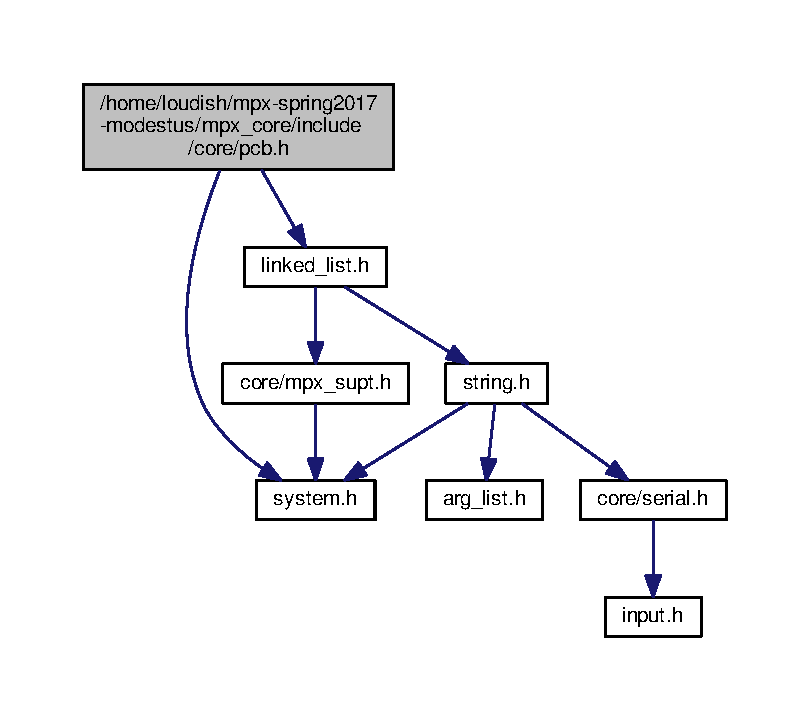
\includegraphics[width=350pt]{pcb_8h__incl}
\end{center}
\end{figure}
This graph shows which files directly or indirectly include this file\+:\nopagebreak
\begin{figure}[H]
\begin{center}
\leavevmode
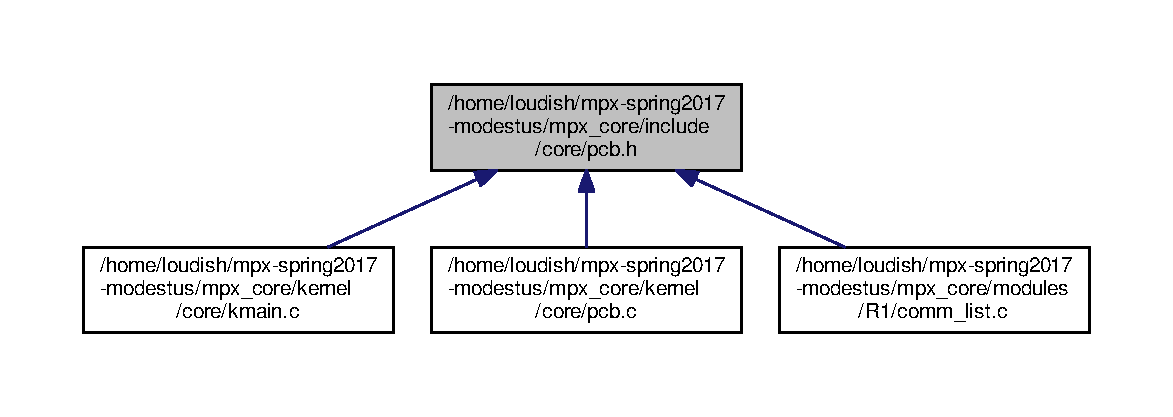
\includegraphics[width=350pt]{pcb_8h__dep__incl}
\end{center}
\end{figure}
\subsection*{Data Structures}
\begin{DoxyCompactItemize}
\item 
struct \hyperlink{structs__pcb__stuct}{pcb\+\_\+t}
\begin{DoxyCompactList}\small\item\em defines the properties of a process control block \end{DoxyCompactList}\end{DoxyCompactItemize}
\subsection*{Macros}
\begin{DoxyCompactItemize}
\item 
\#define \hyperlink{pcb_8h_abb5f1eb47c3ac477582ecc49dc8990ee}{P\+R\+O\+C\+E\+S\+S\+\_\+\+C\+O\+N\+T\+E\+X\+T\+\_\+\+S\+I\+ZE}~(32)
\item 
\#define \hyperlink{pcb_8h_a2dbc13416ed2817701a94e30698cdee3}{P\+R\+O\+C\+E\+S\+S\+\_\+\+S\+T\+A\+C\+K\+\_\+\+S\+I\+ZE}~(1024)
\item 
\#define \hyperlink{pcb_8h_afeaa4736820787d9a22e121d670b9243}{P\+C\+B\+\_\+\+Q\+U\+E\+U\+E\+\_\+\+M\+A\+X\+\_\+\+S\+I\+ZE}~(128)
\item 
\#define \hyperlink{pcb_8h_acd2dea966e4e5b760451b4fcc66f6cce}{P\+R\+O\+C\+E\+S\+S\+\_\+\+M\+A\+X\+\_\+\+N\+A\+M\+E\+\_\+\+L\+E\+N\+G\+TH}~(20)
\end{DoxyCompactItemize}
\subsection*{Typedefs}
\begin{DoxyCompactItemize}
\item 
typedef struct s\+\_\+pcb\+\_\+list \hyperlink{pcb_8h_a58ab885c30f079e61039b7480a7dbfed}{pcb\+Queue\+\_\+t}
\item 
typedef \hyperlink{system_8h_a7c94ea6f8948649f8d181ae55911eeaf}{size\+\_\+t} \hyperlink{pcb_8h_a679b474107b599ed5e2597c8863176dc}{P\+I\+D\+\_\+t}
\begin{DoxyCompactList}\small\item\em P\+I\+D\+\_\+t a type that defines a process operating ID. \end{DoxyCompactList}\item 
typedef \hyperlink{system_8h_a7c94ea6f8948649f8d181ae55911eeaf}{size\+\_\+t} \hyperlink{pcb_8h_aade1badcda6beffd30258586dcad6550}{process\+Priority\+\_\+t}
\begin{DoxyCompactList}\small\item\em process\+Priority\+\_\+t defines a process priority to the system \end{DoxyCompactList}\item 
typedef \hyperlink{system_8h_aba7bc1797add20fe3efdf37ced1182c5}{uint8\+\_\+t} \hyperlink{pcb_8h_aeac19486a8c4d8375298127cee4305b1}{program\+Ptr\+\_\+t}
\begin{DoxyCompactList}\small\item\em program\+Ptr\+\_\+t a pointer to a process\textquotesingle{}s code \end{DoxyCompactList}\item 
typedef \hyperlink{system_8h_aba7bc1797add20fe3efdf37ced1182c5}{uint8\+\_\+t} \hyperlink{pcb_8h_a4f8494f06fbe4ad011320128964be020}{program\+Data\+Ptr\+\_\+t}
\begin{DoxyCompactList}\small\item\em program\+Data\+Ptr\+\_\+t a pointer to a process\textquotesingle{}s data \end{DoxyCompactList}\item 
typedef \hyperlink{system_8h_aba7bc1797add20fe3efdf37ced1182c5}{uint8\+\_\+t} \hyperlink{pcb_8h_a39f696168968032d4df0637fad2ad52c}{process\+Stack\+\_\+t}
\begin{DoxyCompactList}\small\item\em process\+Stack\+\_\+t a pointer to someplace in a process\textquotesingle{}s stack \end{DoxyCompactList}\end{DoxyCompactItemize}
\subsection*{Enumerations}
\begin{DoxyCompactItemize}
\item 
enum \hyperlink{pcb_8h_a7e8c3ee6ff86c6b9d8fd0d2418cc2f8e}{e\+\_\+\+P\+C\+B\+\_\+\+E\+R\+R\+O\+R\+\_\+\+C\+O\+D\+E\+\_\+t} \{ \\*
\hyperlink{pcb_8h_a7e8c3ee6ff86c6b9d8fd0d2418cc2f8eac7f69f7c9e5aea9b8f54cf02870e2bf8}{S\+U\+C\+C\+E\+SS} = 0, 
\hyperlink{pcb_8h_a7e8c3ee6ff86c6b9d8fd0d2418cc2f8ea2fd6f336d08340583bd620a7f5694c90}{E\+R\+R\+OR}, 
\hyperlink{pcb_8h_a7e8c3ee6ff86c6b9d8fd0d2418cc2f8ea5284a4c6f172bebecf5482934910df8c}{E\+R\+R\+O\+R\+\_\+\+P\+C\+B\+\_\+\+N\+O\+T\+\_\+\+F\+O\+U\+ND}, 
\hyperlink{pcb_8h_a7e8c3ee6ff86c6b9d8fd0d2418cc2f8ead49c8157f91ba1ece3849d6d865882a4}{E\+R\+R\+O\+R\+\_\+\+N\+A\+M\+E\+\_\+\+I\+N\+V\+A\+L\+ID}, 
\\*
\hyperlink{pcb_8h_a7e8c3ee6ff86c6b9d8fd0d2418cc2f8ea5a16825b1ce3ee2cb0190cc641921707}{E\+R\+R\+O\+R\+\_\+\+P\+R\+I\+O\+R\+I\+T\+Y\+\_\+\+I\+N\+V\+A\+L\+ID}, 
\hyperlink{pcb_8h_a7e8c3ee6ff86c6b9d8fd0d2418cc2f8ea4190d07ec89ae80f99bfa6b6ffeb692b}{E\+R\+R\+O\+R\+\_\+\+F\+R\+E\+E\+I\+N\+G\+\_\+\+N\+O\+DE}, 
\hyperlink{pcb_8h_a7e8c3ee6ff86c6b9d8fd0d2418cc2f8eae6a47d920115451b70673d54b9d9c164}{E\+R\+R\+O\+R\+\_\+\+F\+R\+E\+E\+I\+N\+G\+\_\+\+S\+T\+A\+CK}, 
\hyperlink{pcb_8h_a7e8c3ee6ff86c6b9d8fd0d2418cc2f8ea65a2fd434138761a45062d90d7381f64}{E\+R\+R\+O\+R\+\_\+\+F\+R\+E\+E\+I\+N\+G\+\_\+\+P\+CB}, 
\\*
\hyperlink{pcb_8h_a7e8c3ee6ff86c6b9d8fd0d2418cc2f8ea2df915668ce49c55a81cd75b8aaa4564}{E\+R\+R\+O\+R\+\_\+\+R\+E\+M\+O\+V\+I\+N\+G\+\_\+\+P\+CB}, 
\hyperlink{pcb_8h_a7e8c3ee6ff86c6b9d8fd0d2418cc2f8ea5f917cfb598da5d3c968757ba14a8ad4}{E\+R\+R\+O\+R\+\_\+\+S\+T\+A\+T\+E\+\_\+\+I\+N\+V\+A\+L\+ID}
 \}\begin{DoxyCompactList}\small\item\em The e\+\_\+\+P\+C\+B\+\_\+\+E\+R\+R\+O\+R\+\_\+\+C\+O\+D\+E\+\_\+t enum defines the return status of functions working with P\+C\+Bs. \end{DoxyCompactList}
\item 
enum \hyperlink{pcb_8h_a8461d6c03c00b03bad59b5a29d27b902}{e\+\_\+\+P\+R\+O\+C\+E\+S\+S\+\_\+\+S\+T\+A\+T\+E\+\_\+t} \{ \\*
\hyperlink{pcb_8h_a8461d6c03c00b03bad59b5a29d27b902a7116db6906963fd0720c4a85be250cf4}{I\+N\+I\+T\+I\+AL}, 
\hyperlink{pcb_8h_a8461d6c03c00b03bad59b5a29d27b902a6564f2f3e15be06b670547bbcaaf0798}{R\+E\+A\+DY}, 
\hyperlink{pcb_8h_a8461d6c03c00b03bad59b5a29d27b902a1061be6c3fb88d32829cba6f6b2be304}{R\+U\+N\+N\+I\+NG}, 
\hyperlink{pcb_8h_a8461d6c03c00b03bad59b5a29d27b902a376c1b6a3f75d283a2efacf737438d61}{B\+L\+O\+C\+K\+ED}, 
\\*
\hyperlink{pcb_8h_a8461d6c03c00b03bad59b5a29d27b902a81cc2296827c731236176fea80701294}{S\+U\+S\+P\+E\+N\+D\+E\+D\+\_\+\+R\+E\+A\+DY}, 
\hyperlink{pcb_8h_a8461d6c03c00b03bad59b5a29d27b902aa4d91165aaa967e74157a23c02725bc7}{S\+U\+S\+P\+E\+N\+D\+E\+D\+\_\+\+B\+L\+O\+C\+K\+ED}, 
\hyperlink{pcb_8h_a8461d6c03c00b03bad59b5a29d27b902a9b2989c4ac8a0f9a7f46528384eaa5c7}{T\+E\+R\+M\+I\+N\+AL}, 
\hyperlink{pcb_8h_a8461d6c03c00b03bad59b5a29d27b902a786a8e9401b8091f65b2afbd342c90f5}{S\+T\+A\+T\+E\+\_\+\+U\+N\+K\+N\+O\+WN}
 \}\begin{DoxyCompactList}\small\item\em The P\+R\+O\+C\+E\+S\+S\+\_\+\+S\+T\+A\+T\+E\+\_\+t enum defines the possible operating states of a process. \end{DoxyCompactList}
\item 
enum \hyperlink{pcb_8h_ab3268ce0bdfc94e5757917d42c73d9f1}{e\+\_\+\+P\+R\+O\+C\+E\+S\+S\+\_\+\+C\+L\+A\+S\+S\+\_\+t} \{ \hyperlink{pcb_8h_ab3268ce0bdfc94e5757917d42c73d9f1a57cc238145ec1361c72c327674c0d754}{S\+Y\+S\+T\+EM}, 
\hyperlink{pcb_8h_ab3268ce0bdfc94e5757917d42c73d9f1a0c6b23d6f956b23100dec45357ff8dc0}{U\+S\+E\+R\+\_\+\+A\+PP}, 
\hyperlink{pcb_8h_ab3268ce0bdfc94e5757917d42c73d9f1a614fd08f9a6cd84e97785eb2c551dafe}{C\+L\+A\+S\+S\+\_\+\+U\+N\+K\+N\+O\+WN}
 \}\begin{DoxyCompactList}\small\item\em The P\+R\+O\+C\+E\+S\+S\+\_\+\+C\+L\+A\+S\+S\+\_\+t enum defines the operating class of the process. \end{DoxyCompactList}
\end{DoxyCompactItemize}
\subsection*{Functions}
\begin{DoxyCompactItemize}
\item 
\hyperlink{structpcb__t}{pcb\+\_\+t} $\ast$ \hyperlink{pcb_8h_a5c2a9f7bca10a6d45287ce6834b7167c}{allocate\+P\+CB} (void)
\begin{DoxyCompactList}\small\item\em allocate\+P\+CB allocate new memory for a \hyperlink{structpcb__t}{pcb\+\_\+t} \end{DoxyCompactList}\item 
\hyperlink{pcb_8h_a7e8c3ee6ff86c6b9d8fd0d2418cc2f8e}{e\+\_\+\+P\+C\+B\+\_\+\+E\+R\+R\+O\+R\+\_\+\+C\+O\+D\+E\+\_\+t} \hyperlink{pcb_8h_aa2fdf62a032353fbef2792502860709b}{free\+P\+CB} (\hyperlink{structpcb__t}{pcb\+\_\+t} $\ast$pcb\+To\+Free)
\begin{DoxyCompactList}\small\item\em free\+P\+CB free all associated memory with the P\+CB, including the stack and other pointers \end{DoxyCompactList}\item 
\hyperlink{structpcb__t}{pcb\+\_\+t} $\ast$ \hyperlink{pcb_8h_a9928a07bb6f59213464656fdab142e70}{setup\+P\+CB} (const char $\ast$process\+Name, \hyperlink{pcb_8h_ab3268ce0bdfc94e5757917d42c73d9f1}{e\+\_\+\+P\+R\+O\+C\+E\+S\+S\+\_\+\+C\+L\+A\+S\+S\+\_\+t} process\+Class, \hyperlink{pcb_8h_aade1badcda6beffd30258586dcad6550}{process\+Priority\+\_\+t} process\+Priority)
\begin{DoxyCompactList}\small\item\em setup\+P\+CB calls allocate\+P\+CB, initializes the P\+CB with the arguments and sets it state to ready \end{DoxyCompactList}\item 
\hyperlink{structpcb__t}{pcb\+\_\+t} $\ast$ \hyperlink{pcb_8h_a3ddbd6b7d5425cfb586dabc05862e9b1}{find\+P\+CB} (const char $\ast$process\+Name)
\begin{DoxyCompactList}\small\item\em find\+P\+CB will search all queues for the P\+CB with the input name \end{DoxyCompactList}\item 
void \hyperlink{pcb_8h_aa1e16d4087c6b2a5acf3aff5a3f339ee}{insert\+P\+CB} (\hyperlink{structpcb__t}{pcb\+\_\+t} $\ast$pcb\+To\+Insert)
\begin{DoxyCompactList}\small\item\em insert\+P\+CB insert the P\+CB into the queue represented by the process state, following each queue\textquotesingle{}s rules \end{DoxyCompactList}\item 
\hyperlink{pcb_8h_a7e8c3ee6ff86c6b9d8fd0d2418cc2f8e}{e\+\_\+\+P\+C\+B\+\_\+\+E\+R\+R\+O\+R\+\_\+\+C\+O\+D\+E\+\_\+t} \hyperlink{pcb_8h_aa7ccac95996427cc60aaee4eec35caf4}{remove\+P\+CB} (\hyperlink{structpcb__t}{pcb\+\_\+t} $\ast$pcb\+To\+Remove)
\begin{DoxyCompactList}\small\item\em remove\+P\+CB remove the input P\+CB from its associated queue \end{DoxyCompactList}\item 
\hyperlink{pcb_8h_a8461d6c03c00b03bad59b5a29d27b902}{e\+\_\+\+P\+R\+O\+C\+E\+S\+S\+\_\+\+S\+T\+A\+T\+E\+\_\+t} \hyperlink{group___r2_gae34a580c5336a0d5f2a0589f41f25fa2}{get\+State} (const char $\ast$name)
\begin{DoxyCompactList}\small\item\em get\+State gets the current state of the process \end{DoxyCompactList}\item 
int \hyperlink{pcb_8h_a8c657cc0a82e51f22c2b601cc961169e}{pcb\+Search\+Func} (void $\ast$pcb, void $\ast$name\+To\+Find)
\begin{DoxyCompactList}\small\item\em pcb\+Search\+Func pcb search function for linked list. All pcb linked\+Lists use this function for searching See \hyperlink{linked__list_8c_a12e5138ac02af0f6b42ff2f1b29c610a}{Linked List documentation} for a description of a list search function \end{DoxyCompactList}\item 
int \hyperlink{pcb_8h_ac5785e5f577e5f50d2de01aa0683c275}{priority\+Insert\+Func} (void $\ast$pcb1, void $\ast$pcb2)
\begin{DoxyCompactList}\small\item\em priority\+Insert\+Func function that inserts pcbs into new pcb queues ordered by the pcbs\textquotesingle{} priority. See \hyperlink{linked__list_8c_a45d030386936adffa3eb5586ce93d131}{Linked List documentation} for a better description of a list insert function. \end{DoxyCompactList}\item 
int \hyperlink{pcb_8h_a30717aca6066b99d5d73c6fda5b438e6}{fifo\+Insert\+Func} (void $\ast$pcb1, void $\ast$pcb2)
\begin{DoxyCompactList}\small\item\em priority\+Insert\+Func function that inserts pcbs into new pcb queues ordered by the sequence of arrival. See \hyperlink{linked__list_8c_a45d030386936adffa3eb5586ce93d131}{Linked List documentation} for a better description of a list insert function. \end{DoxyCompactList}\item 
void \hyperlink{pcb_8h_a8649777d644ec839c0d02d966f068f45}{init\+P\+C\+B\+Queues} (void)
\begin{DoxyCompactList}\small\item\em init\+P\+C\+B\+Queues initlize the queues for each process queue. This function calls the list init function and sets the function pointers for each list \end{DoxyCompactList}\item 
void \hyperlink{pcb_8h_adc4d10af06448eb7a046bacfc2918ea2}{pcb\+Test} (void)
\begin{DoxyCompactList}\small\item\em pcb\+Test a simple test case function to show pcb queue functionality \end{DoxyCompactList}\item 
\hyperlink{pcb_8h_a7e8c3ee6ff86c6b9d8fd0d2418cc2f8e}{e\+\_\+\+P\+C\+B\+\_\+\+E\+R\+R\+O\+R\+\_\+\+C\+O\+D\+E\+\_\+t} \hyperlink{group___r2_ga83a5983d76f08725aadc23bf47930436}{change\+Process\+State} (const char $\ast$name, \hyperlink{pcb_8h_a8461d6c03c00b03bad59b5a29d27b902}{e\+\_\+\+P\+R\+O\+C\+E\+S\+S\+\_\+\+S\+T\+A\+T\+E\+\_\+t} state)
\begin{DoxyCompactList}\small\item\em change\+Process\+State changes the state of the process being called \end{DoxyCompactList}\item 
int \hyperlink{group___r2_ga1e42e70128de8086a07dbcd97e000942}{is\+Suspended} (\hyperlink{pcb_8h_a8461d6c03c00b03bad59b5a29d27b902}{e\+\_\+\+P\+R\+O\+C\+E\+S\+S\+\_\+\+S\+T\+A\+T\+E\+\_\+t} state)
\begin{DoxyCompactList}\small\item\em is\+Suspended gets the suspension status of the process \end{DoxyCompactList}\item 
const char $\ast$ \hyperlink{group___r2_ga834927e89e94c123a0ec5322b11b0161}{error\+To\+String} (\hyperlink{pcb_8h_a7e8c3ee6ff86c6b9d8fd0d2418cc2f8e}{e\+\_\+\+P\+C\+B\+\_\+\+E\+R\+R\+O\+R\+\_\+\+C\+O\+D\+E\+\_\+t} error)
\begin{DoxyCompactList}\small\item\em error\+To\+String creates a string form of the error passed in \end{DoxyCompactList}\item 
const char $\ast$ \hyperlink{group___r2_gac38459f8731293f12b7fb0170c923471}{class\+To\+String} (\hyperlink{pcb_8h_ab3268ce0bdfc94e5757917d42c73d9f1}{e\+\_\+\+P\+R\+O\+C\+E\+S\+S\+\_\+\+C\+L\+A\+S\+S\+\_\+t} process\+Class)
\begin{DoxyCompactList}\small\item\em class\+To\+String creates a string form of the class passed in \end{DoxyCompactList}\item 
const char $\ast$ \hyperlink{group___r2_ga8667e4228a987f7d43e598f9855e9a52}{state\+To\+String} (\hyperlink{pcb_8h_a8461d6c03c00b03bad59b5a29d27b902}{e\+\_\+\+P\+R\+O\+C\+E\+S\+S\+\_\+\+S\+T\+A\+T\+E\+\_\+t} state)
\begin{DoxyCompactList}\small\item\em state\+To\+String creates a string form of the state passed in \end{DoxyCompactList}\item 
\hyperlink{pcb_8h_ab3268ce0bdfc94e5757917d42c73d9f1}{e\+\_\+\+P\+R\+O\+C\+E\+S\+S\+\_\+\+C\+L\+A\+S\+S\+\_\+t} \hyperlink{group___r2_gae81b3dd13059be0733193c53681ca440}{string\+To\+Class} (const char $\ast$stringified\+Class)
\begin{DoxyCompactList}\small\item\em string\+To\+Class returns the enum representation of a string \end{DoxyCompactList}\item 
void \hyperlink{group___r2_ga819c31d0b376ca33ed371253585f9f80}{print\+P\+C\+B\+Func} (void $\ast$pcb)
\begin{DoxyCompactList}\small\item\em print\+P\+C\+B\+Func prints the status of a process \end{DoxyCompactList}\end{DoxyCompactItemize}
\subsection*{Variables}
\begin{DoxyCompactItemize}
\item 
\hyperlink{structlinked_list__t}{linked\+List\+\_\+t} \hyperlink{pcb_8h_a7b1bca867586a0a58222b805dbe3be28}{ready\+Queue}
\item 
\hyperlink{structlinked_list__t}{linked\+List\+\_\+t} \hyperlink{pcb_8h_aa3eb63b40a5cf1eb03b494f7ddd1af2a}{blocked\+Queue}
\item 
\hyperlink{structlinked_list__t}{linked\+List\+\_\+t} \hyperlink{pcb_8h_a95c66b02e576aabe04df3fdc9e981fc3}{suspended\+Ready\+Queue}
\item 
\hyperlink{structlinked_list__t}{linked\+List\+\_\+t} \hyperlink{pcb_8h_ae83c9a71ab217215db8dfe3eb9c94e8e}{suspended\+Blocked\+Queue}
\item 
\hyperlink{structlinked_list__t}{linked\+List\+\_\+t} \hyperlink{pcb_8h_a6d936c9220673197cf184738a19b64c9}{total\+Process\+List}
\end{DoxyCompactItemize}


\subsection{Macro Definition Documentation}
\index{pcb.\+h@{pcb.\+h}!P\+C\+B\+\_\+\+Q\+U\+E\+U\+E\+\_\+\+M\+A\+X\+\_\+\+S\+I\+ZE@{P\+C\+B\+\_\+\+Q\+U\+E\+U\+E\+\_\+\+M\+A\+X\+\_\+\+S\+I\+ZE}}
\index{P\+C\+B\+\_\+\+Q\+U\+E\+U\+E\+\_\+\+M\+A\+X\+\_\+\+S\+I\+ZE@{P\+C\+B\+\_\+\+Q\+U\+E\+U\+E\+\_\+\+M\+A\+X\+\_\+\+S\+I\+ZE}!pcb.\+h@{pcb.\+h}}
\subsubsection[{\texorpdfstring{P\+C\+B\+\_\+\+Q\+U\+E\+U\+E\+\_\+\+M\+A\+X\+\_\+\+S\+I\+ZE}{PCB_QUEUE_MAX_SIZE}}]{\setlength{\rightskip}{0pt plus 5cm}\#define P\+C\+B\+\_\+\+Q\+U\+E\+U\+E\+\_\+\+M\+A\+X\+\_\+\+S\+I\+ZE~(128)}\hypertarget{pcb_8h_afeaa4736820787d9a22e121d670b9243}{}\label{pcb_8h_afeaa4736820787d9a22e121d670b9243}


Definition at line 18 of file pcb.\+h.

\index{pcb.\+h@{pcb.\+h}!P\+R\+O\+C\+E\+S\+S\+\_\+\+C\+O\+N\+T\+E\+X\+T\+\_\+\+S\+I\+ZE@{P\+R\+O\+C\+E\+S\+S\+\_\+\+C\+O\+N\+T\+E\+X\+T\+\_\+\+S\+I\+ZE}}
\index{P\+R\+O\+C\+E\+S\+S\+\_\+\+C\+O\+N\+T\+E\+X\+T\+\_\+\+S\+I\+ZE@{P\+R\+O\+C\+E\+S\+S\+\_\+\+C\+O\+N\+T\+E\+X\+T\+\_\+\+S\+I\+ZE}!pcb.\+h@{pcb.\+h}}
\subsubsection[{\texorpdfstring{P\+R\+O\+C\+E\+S\+S\+\_\+\+C\+O\+N\+T\+E\+X\+T\+\_\+\+S\+I\+ZE}{PROCESS_CONTEXT_SIZE}}]{\setlength{\rightskip}{0pt plus 5cm}\#define P\+R\+O\+C\+E\+S\+S\+\_\+\+C\+O\+N\+T\+E\+X\+T\+\_\+\+S\+I\+ZE~(32)}\hypertarget{pcb_8h_abb5f1eb47c3ac477582ecc49dc8990ee}{}\label{pcb_8h_abb5f1eb47c3ac477582ecc49dc8990ee}


Definition at line 16 of file pcb.\+h.

\index{pcb.\+h@{pcb.\+h}!P\+R\+O\+C\+E\+S\+S\+\_\+\+M\+A\+X\+\_\+\+N\+A\+M\+E\+\_\+\+L\+E\+N\+G\+TH@{P\+R\+O\+C\+E\+S\+S\+\_\+\+M\+A\+X\+\_\+\+N\+A\+M\+E\+\_\+\+L\+E\+N\+G\+TH}}
\index{P\+R\+O\+C\+E\+S\+S\+\_\+\+M\+A\+X\+\_\+\+N\+A\+M\+E\+\_\+\+L\+E\+N\+G\+TH@{P\+R\+O\+C\+E\+S\+S\+\_\+\+M\+A\+X\+\_\+\+N\+A\+M\+E\+\_\+\+L\+E\+N\+G\+TH}!pcb.\+h@{pcb.\+h}}
\subsubsection[{\texorpdfstring{P\+R\+O\+C\+E\+S\+S\+\_\+\+M\+A\+X\+\_\+\+N\+A\+M\+E\+\_\+\+L\+E\+N\+G\+TH}{PROCESS_MAX_NAME_LENGTH}}]{\setlength{\rightskip}{0pt plus 5cm}\#define P\+R\+O\+C\+E\+S\+S\+\_\+\+M\+A\+X\+\_\+\+N\+A\+M\+E\+\_\+\+L\+E\+N\+G\+TH~(20)}\hypertarget{pcb_8h_acd2dea966e4e5b760451b4fcc66f6cce}{}\label{pcb_8h_acd2dea966e4e5b760451b4fcc66f6cce}


Definition at line 19 of file pcb.\+h.



Referenced by setup\+P\+C\+B().

\index{pcb.\+h@{pcb.\+h}!P\+R\+O\+C\+E\+S\+S\+\_\+\+S\+T\+A\+C\+K\+\_\+\+S\+I\+ZE@{P\+R\+O\+C\+E\+S\+S\+\_\+\+S\+T\+A\+C\+K\+\_\+\+S\+I\+ZE}}
\index{P\+R\+O\+C\+E\+S\+S\+\_\+\+S\+T\+A\+C\+K\+\_\+\+S\+I\+ZE@{P\+R\+O\+C\+E\+S\+S\+\_\+\+S\+T\+A\+C\+K\+\_\+\+S\+I\+ZE}!pcb.\+h@{pcb.\+h}}
\subsubsection[{\texorpdfstring{P\+R\+O\+C\+E\+S\+S\+\_\+\+S\+T\+A\+C\+K\+\_\+\+S\+I\+ZE}{PROCESS_STACK_SIZE}}]{\setlength{\rightskip}{0pt plus 5cm}\#define P\+R\+O\+C\+E\+S\+S\+\_\+\+S\+T\+A\+C\+K\+\_\+\+S\+I\+ZE~(1024)}\hypertarget{pcb_8h_a2dbc13416ed2817701a94e30698cdee3}{}\label{pcb_8h_a2dbc13416ed2817701a94e30698cdee3}


Definition at line 17 of file pcb.\+h.



\subsection{Typedef Documentation}
\index{pcb.\+h@{pcb.\+h}!pcb\+Queue\+\_\+t@{pcb\+Queue\+\_\+t}}
\index{pcb\+Queue\+\_\+t@{pcb\+Queue\+\_\+t}!pcb.\+h@{pcb.\+h}}
\subsubsection[{\texorpdfstring{pcb\+Queue\+\_\+t}{pcbQueue_t}}]{\setlength{\rightskip}{0pt plus 5cm}typedef struct s\+\_\+pcb\+\_\+list {\bf pcb\+Queue\+\_\+t}}\hypertarget{pcb_8h_a58ab885c30f079e61039b7480a7dbfed}{}\label{pcb_8h_a58ab885c30f079e61039b7480a7dbfed}


Definition at line 57 of file pcb.\+h.

\index{pcb.\+h@{pcb.\+h}!P\+I\+D\+\_\+t@{P\+I\+D\+\_\+t}}
\index{P\+I\+D\+\_\+t@{P\+I\+D\+\_\+t}!pcb.\+h@{pcb.\+h}}
\subsubsection[{\texorpdfstring{P\+I\+D\+\_\+t}{PID_t}}]{\setlength{\rightskip}{0pt plus 5cm}typedef {\bf size\+\_\+t} {\bf P\+I\+D\+\_\+t}}\hypertarget{pcb_8h_a679b474107b599ed5e2597c8863176dc}{}\label{pcb_8h_a679b474107b599ed5e2597c8863176dc}


P\+I\+D\+\_\+t a type that defines a process operating ID. 



Definition at line 62 of file pcb.\+h.

\index{pcb.\+h@{pcb.\+h}!process\+Priority\+\_\+t@{process\+Priority\+\_\+t}}
\index{process\+Priority\+\_\+t@{process\+Priority\+\_\+t}!pcb.\+h@{pcb.\+h}}
\subsubsection[{\texorpdfstring{process\+Priority\+\_\+t}{processPriority_t}}]{\setlength{\rightskip}{0pt plus 5cm}typedef {\bf size\+\_\+t} {\bf process\+Priority\+\_\+t}}\hypertarget{pcb_8h_aade1badcda6beffd30258586dcad6550}{}\label{pcb_8h_aade1badcda6beffd30258586dcad6550}


process\+Priority\+\_\+t defines a process priority to the system 



Definition at line 67 of file pcb.\+h.

\index{pcb.\+h@{pcb.\+h}!process\+Stack\+\_\+t@{process\+Stack\+\_\+t}}
\index{process\+Stack\+\_\+t@{process\+Stack\+\_\+t}!pcb.\+h@{pcb.\+h}}
\subsubsection[{\texorpdfstring{process\+Stack\+\_\+t}{processStack_t}}]{\setlength{\rightskip}{0pt plus 5cm}typedef {\bf uint8\+\_\+t} {\bf process\+Stack\+\_\+t}}\hypertarget{pcb_8h_a39f696168968032d4df0637fad2ad52c}{}\label{pcb_8h_a39f696168968032d4df0637fad2ad52c}


process\+Stack\+\_\+t a pointer to someplace in a process\textquotesingle{}s stack 



Definition at line 82 of file pcb.\+h.

\index{pcb.\+h@{pcb.\+h}!program\+Data\+Ptr\+\_\+t@{program\+Data\+Ptr\+\_\+t}}
\index{program\+Data\+Ptr\+\_\+t@{program\+Data\+Ptr\+\_\+t}!pcb.\+h@{pcb.\+h}}
\subsubsection[{\texorpdfstring{program\+Data\+Ptr\+\_\+t}{programDataPtr_t}}]{\setlength{\rightskip}{0pt plus 5cm}typedef {\bf uint8\+\_\+t} {\bf program\+Data\+Ptr\+\_\+t}}\hypertarget{pcb_8h_a4f8494f06fbe4ad011320128964be020}{}\label{pcb_8h_a4f8494f06fbe4ad011320128964be020}


program\+Data\+Ptr\+\_\+t a pointer to a process\textquotesingle{}s data 



Definition at line 77 of file pcb.\+h.

\index{pcb.\+h@{pcb.\+h}!program\+Ptr\+\_\+t@{program\+Ptr\+\_\+t}}
\index{program\+Ptr\+\_\+t@{program\+Ptr\+\_\+t}!pcb.\+h@{pcb.\+h}}
\subsubsection[{\texorpdfstring{program\+Ptr\+\_\+t}{programPtr_t}}]{\setlength{\rightskip}{0pt plus 5cm}typedef {\bf uint8\+\_\+t} {\bf program\+Ptr\+\_\+t}}\hypertarget{pcb_8h_aeac19486a8c4d8375298127cee4305b1}{}\label{pcb_8h_aeac19486a8c4d8375298127cee4305b1}


program\+Ptr\+\_\+t a pointer to a process\textquotesingle{}s code 



Definition at line 72 of file pcb.\+h.



\subsection{Enumeration Type Documentation}
\index{pcb.\+h@{pcb.\+h}!e\+\_\+\+P\+C\+B\+\_\+\+E\+R\+R\+O\+R\+\_\+\+C\+O\+D\+E\+\_\+t@{e\+\_\+\+P\+C\+B\+\_\+\+E\+R\+R\+O\+R\+\_\+\+C\+O\+D\+E\+\_\+t}}
\index{e\+\_\+\+P\+C\+B\+\_\+\+E\+R\+R\+O\+R\+\_\+\+C\+O\+D\+E\+\_\+t@{e\+\_\+\+P\+C\+B\+\_\+\+E\+R\+R\+O\+R\+\_\+\+C\+O\+D\+E\+\_\+t}!pcb.\+h@{pcb.\+h}}
\subsubsection[{\texorpdfstring{e\+\_\+\+P\+C\+B\+\_\+\+E\+R\+R\+O\+R\+\_\+\+C\+O\+D\+E\+\_\+t}{e_PCB_ERROR_CODE_t}}]{\setlength{\rightskip}{0pt plus 5cm}enum {\bf e\+\_\+\+P\+C\+B\+\_\+\+E\+R\+R\+O\+R\+\_\+\+C\+O\+D\+E\+\_\+t}}\hypertarget{pcb_8h_a7e8c3ee6ff86c6b9d8fd0d2418cc2f8e}{}\label{pcb_8h_a7e8c3ee6ff86c6b9d8fd0d2418cc2f8e}


The e\+\_\+\+P\+C\+B\+\_\+\+E\+R\+R\+O\+R\+\_\+\+C\+O\+D\+E\+\_\+t enum defines the return status of functions working with P\+C\+Bs. 

\begin{Desc}
\item[Enumerator]\par
\begin{description}
\index{S\+U\+C\+C\+E\+SS@{S\+U\+C\+C\+E\+SS}!pcb.\+h@{pcb.\+h}}\index{pcb.\+h@{pcb.\+h}!S\+U\+C\+C\+E\+SS@{S\+U\+C\+C\+E\+SS}}\item[{\em 
S\+U\+C\+C\+E\+SS\hypertarget{pcb_8h_a7e8c3ee6ff86c6b9d8fd0d2418cc2f8eac7f69f7c9e5aea9b8f54cf02870e2bf8}{}\label{pcb_8h_a7e8c3ee6ff86c6b9d8fd0d2418cc2f8eac7f69f7c9e5aea9b8f54cf02870e2bf8}
}]\index{E\+R\+R\+OR@{E\+R\+R\+OR}!pcb.\+h@{pcb.\+h}}\index{pcb.\+h@{pcb.\+h}!E\+R\+R\+OR@{E\+R\+R\+OR}}\item[{\em 
E\+R\+R\+OR\hypertarget{pcb_8h_a7e8c3ee6ff86c6b9d8fd0d2418cc2f8ea2fd6f336d08340583bd620a7f5694c90}{}\label{pcb_8h_a7e8c3ee6ff86c6b9d8fd0d2418cc2f8ea2fd6f336d08340583bd620a7f5694c90}
}]\index{E\+R\+R\+O\+R\+\_\+\+P\+C\+B\+\_\+\+N\+O\+T\+\_\+\+F\+O\+U\+ND@{E\+R\+R\+O\+R\+\_\+\+P\+C\+B\+\_\+\+N\+O\+T\+\_\+\+F\+O\+U\+ND}!pcb.\+h@{pcb.\+h}}\index{pcb.\+h@{pcb.\+h}!E\+R\+R\+O\+R\+\_\+\+P\+C\+B\+\_\+\+N\+O\+T\+\_\+\+F\+O\+U\+ND@{E\+R\+R\+O\+R\+\_\+\+P\+C\+B\+\_\+\+N\+O\+T\+\_\+\+F\+O\+U\+ND}}\item[{\em 
E\+R\+R\+O\+R\+\_\+\+P\+C\+B\+\_\+\+N\+O\+T\+\_\+\+F\+O\+U\+ND\hypertarget{pcb_8h_a7e8c3ee6ff86c6b9d8fd0d2418cc2f8ea5284a4c6f172bebecf5482934910df8c}{}\label{pcb_8h_a7e8c3ee6ff86c6b9d8fd0d2418cc2f8ea5284a4c6f172bebecf5482934910df8c}
}]\index{E\+R\+R\+O\+R\+\_\+\+N\+A\+M\+E\+\_\+\+I\+N\+V\+A\+L\+ID@{E\+R\+R\+O\+R\+\_\+\+N\+A\+M\+E\+\_\+\+I\+N\+V\+A\+L\+ID}!pcb.\+h@{pcb.\+h}}\index{pcb.\+h@{pcb.\+h}!E\+R\+R\+O\+R\+\_\+\+N\+A\+M\+E\+\_\+\+I\+N\+V\+A\+L\+ID@{E\+R\+R\+O\+R\+\_\+\+N\+A\+M\+E\+\_\+\+I\+N\+V\+A\+L\+ID}}\item[{\em 
E\+R\+R\+O\+R\+\_\+\+N\+A\+M\+E\+\_\+\+I\+N\+V\+A\+L\+ID\hypertarget{pcb_8h_a7e8c3ee6ff86c6b9d8fd0d2418cc2f8ead49c8157f91ba1ece3849d6d865882a4}{}\label{pcb_8h_a7e8c3ee6ff86c6b9d8fd0d2418cc2f8ead49c8157f91ba1ece3849d6d865882a4}
}]\index{E\+R\+R\+O\+R\+\_\+\+P\+R\+I\+O\+R\+I\+T\+Y\+\_\+\+I\+N\+V\+A\+L\+ID@{E\+R\+R\+O\+R\+\_\+\+P\+R\+I\+O\+R\+I\+T\+Y\+\_\+\+I\+N\+V\+A\+L\+ID}!pcb.\+h@{pcb.\+h}}\index{pcb.\+h@{pcb.\+h}!E\+R\+R\+O\+R\+\_\+\+P\+R\+I\+O\+R\+I\+T\+Y\+\_\+\+I\+N\+V\+A\+L\+ID@{E\+R\+R\+O\+R\+\_\+\+P\+R\+I\+O\+R\+I\+T\+Y\+\_\+\+I\+N\+V\+A\+L\+ID}}\item[{\em 
E\+R\+R\+O\+R\+\_\+\+P\+R\+I\+O\+R\+I\+T\+Y\+\_\+\+I\+N\+V\+A\+L\+ID\hypertarget{pcb_8h_a7e8c3ee6ff86c6b9d8fd0d2418cc2f8ea5a16825b1ce3ee2cb0190cc641921707}{}\label{pcb_8h_a7e8c3ee6ff86c6b9d8fd0d2418cc2f8ea5a16825b1ce3ee2cb0190cc641921707}
}]\index{E\+R\+R\+O\+R\+\_\+\+F\+R\+E\+E\+I\+N\+G\+\_\+\+N\+O\+DE@{E\+R\+R\+O\+R\+\_\+\+F\+R\+E\+E\+I\+N\+G\+\_\+\+N\+O\+DE}!pcb.\+h@{pcb.\+h}}\index{pcb.\+h@{pcb.\+h}!E\+R\+R\+O\+R\+\_\+\+F\+R\+E\+E\+I\+N\+G\+\_\+\+N\+O\+DE@{E\+R\+R\+O\+R\+\_\+\+F\+R\+E\+E\+I\+N\+G\+\_\+\+N\+O\+DE}}\item[{\em 
E\+R\+R\+O\+R\+\_\+\+F\+R\+E\+E\+I\+N\+G\+\_\+\+N\+O\+DE\hypertarget{pcb_8h_a7e8c3ee6ff86c6b9d8fd0d2418cc2f8ea4190d07ec89ae80f99bfa6b6ffeb692b}{}\label{pcb_8h_a7e8c3ee6ff86c6b9d8fd0d2418cc2f8ea4190d07ec89ae80f99bfa6b6ffeb692b}
}]\index{E\+R\+R\+O\+R\+\_\+\+F\+R\+E\+E\+I\+N\+G\+\_\+\+S\+T\+A\+CK@{E\+R\+R\+O\+R\+\_\+\+F\+R\+E\+E\+I\+N\+G\+\_\+\+S\+T\+A\+CK}!pcb.\+h@{pcb.\+h}}\index{pcb.\+h@{pcb.\+h}!E\+R\+R\+O\+R\+\_\+\+F\+R\+E\+E\+I\+N\+G\+\_\+\+S\+T\+A\+CK@{E\+R\+R\+O\+R\+\_\+\+F\+R\+E\+E\+I\+N\+G\+\_\+\+S\+T\+A\+CK}}\item[{\em 
E\+R\+R\+O\+R\+\_\+\+F\+R\+E\+E\+I\+N\+G\+\_\+\+S\+T\+A\+CK\hypertarget{pcb_8h_a7e8c3ee6ff86c6b9d8fd0d2418cc2f8eae6a47d920115451b70673d54b9d9c164}{}\label{pcb_8h_a7e8c3ee6ff86c6b9d8fd0d2418cc2f8eae6a47d920115451b70673d54b9d9c164}
}]\index{E\+R\+R\+O\+R\+\_\+\+F\+R\+E\+E\+I\+N\+G\+\_\+\+P\+CB@{E\+R\+R\+O\+R\+\_\+\+F\+R\+E\+E\+I\+N\+G\+\_\+\+P\+CB}!pcb.\+h@{pcb.\+h}}\index{pcb.\+h@{pcb.\+h}!E\+R\+R\+O\+R\+\_\+\+F\+R\+E\+E\+I\+N\+G\+\_\+\+P\+CB@{E\+R\+R\+O\+R\+\_\+\+F\+R\+E\+E\+I\+N\+G\+\_\+\+P\+CB}}\item[{\em 
E\+R\+R\+O\+R\+\_\+\+F\+R\+E\+E\+I\+N\+G\+\_\+\+P\+CB\hypertarget{pcb_8h_a7e8c3ee6ff86c6b9d8fd0d2418cc2f8ea65a2fd434138761a45062d90d7381f64}{}\label{pcb_8h_a7e8c3ee6ff86c6b9d8fd0d2418cc2f8ea65a2fd434138761a45062d90d7381f64}
}]\index{E\+R\+R\+O\+R\+\_\+\+R\+E\+M\+O\+V\+I\+N\+G\+\_\+\+P\+CB@{E\+R\+R\+O\+R\+\_\+\+R\+E\+M\+O\+V\+I\+N\+G\+\_\+\+P\+CB}!pcb.\+h@{pcb.\+h}}\index{pcb.\+h@{pcb.\+h}!E\+R\+R\+O\+R\+\_\+\+R\+E\+M\+O\+V\+I\+N\+G\+\_\+\+P\+CB@{E\+R\+R\+O\+R\+\_\+\+R\+E\+M\+O\+V\+I\+N\+G\+\_\+\+P\+CB}}\item[{\em 
E\+R\+R\+O\+R\+\_\+\+R\+E\+M\+O\+V\+I\+N\+G\+\_\+\+P\+CB\hypertarget{pcb_8h_a7e8c3ee6ff86c6b9d8fd0d2418cc2f8ea2df915668ce49c55a81cd75b8aaa4564}{}\label{pcb_8h_a7e8c3ee6ff86c6b9d8fd0d2418cc2f8ea2df915668ce49c55a81cd75b8aaa4564}
}]\index{E\+R\+R\+O\+R\+\_\+\+S\+T\+A\+T\+E\+\_\+\+I\+N\+V\+A\+L\+ID@{E\+R\+R\+O\+R\+\_\+\+S\+T\+A\+T\+E\+\_\+\+I\+N\+V\+A\+L\+ID}!pcb.\+h@{pcb.\+h}}\index{pcb.\+h@{pcb.\+h}!E\+R\+R\+O\+R\+\_\+\+S\+T\+A\+T\+E\+\_\+\+I\+N\+V\+A\+L\+ID@{E\+R\+R\+O\+R\+\_\+\+S\+T\+A\+T\+E\+\_\+\+I\+N\+V\+A\+L\+ID}}\item[{\em 
E\+R\+R\+O\+R\+\_\+\+S\+T\+A\+T\+E\+\_\+\+I\+N\+V\+A\+L\+ID\hypertarget{pcb_8h_a7e8c3ee6ff86c6b9d8fd0d2418cc2f8ea5f917cfb598da5d3c968757ba14a8ad4}{}\label{pcb_8h_a7e8c3ee6ff86c6b9d8fd0d2418cc2f8ea5f917cfb598da5d3c968757ba14a8ad4}
}]\end{description}
\end{Desc}


Definition at line 31 of file pcb.\+h.


\begin{DoxyCode}
31              \{\hyperlink{pcb_8h_a7e8c3ee6ff86c6b9d8fd0d2418cc2f8eac7f69f7c9e5aea9b8f54cf02870e2bf8}{SUCCESS} = 0, \hyperlink{pcb_8h_a7e8c3ee6ff86c6b9d8fd0d2418cc2f8ea2fd6f336d08340583bd620a7f5694c90}{ERROR}, \hyperlink{pcb_8h_a7e8c3ee6ff86c6b9d8fd0d2418cc2f8ea5284a4c6f172bebecf5482934910df8c}{ERROR\_PCB\_NOT\_FOUND}, 
      \hyperlink{pcb_8h_a7e8c3ee6ff86c6b9d8fd0d2418cc2f8ead49c8157f91ba1ece3849d6d865882a4}{ERROR\_NAME\_INVALID}, \hyperlink{pcb_8h_a7e8c3ee6ff86c6b9d8fd0d2418cc2f8ea5a16825b1ce3ee2cb0190cc641921707}{ERROR\_PRIORITY\_INVALID},
32                             \hyperlink{pcb_8h_a7e8c3ee6ff86c6b9d8fd0d2418cc2f8ea4190d07ec89ae80f99bfa6b6ffeb692b}{ERROR\_FREEING\_NODE}, 
      \hyperlink{pcb_8h_a7e8c3ee6ff86c6b9d8fd0d2418cc2f8eae6a47d920115451b70673d54b9d9c164}{ERROR\_FREEING\_STACK}, \hyperlink{pcb_8h_a7e8c3ee6ff86c6b9d8fd0d2418cc2f8ea65a2fd434138761a45062d90d7381f64}{ERROR\_FREEING\_PCB}, 
      \hyperlink{pcb_8h_a7e8c3ee6ff86c6b9d8fd0d2418cc2f8ea2df915668ce49c55a81cd75b8aaa4564}{ERROR\_REMOVING\_PCB}, \hyperlink{pcb_8h_a7e8c3ee6ff86c6b9d8fd0d2418cc2f8ea5f917cfb598da5d3c968757ba14a8ad4}{ERROR\_STATE\_INVALID}\}
\end{DoxyCode}
\index{pcb.\+h@{pcb.\+h}!e\+\_\+\+P\+R\+O\+C\+E\+S\+S\+\_\+\+C\+L\+A\+S\+S\+\_\+t@{e\+\_\+\+P\+R\+O\+C\+E\+S\+S\+\_\+\+C\+L\+A\+S\+S\+\_\+t}}
\index{e\+\_\+\+P\+R\+O\+C\+E\+S\+S\+\_\+\+C\+L\+A\+S\+S\+\_\+t@{e\+\_\+\+P\+R\+O\+C\+E\+S\+S\+\_\+\+C\+L\+A\+S\+S\+\_\+t}!pcb.\+h@{pcb.\+h}}
\subsubsection[{\texorpdfstring{e\+\_\+\+P\+R\+O\+C\+E\+S\+S\+\_\+\+C\+L\+A\+S\+S\+\_\+t}{e_PROCESS_CLASS_t}}]{\setlength{\rightskip}{0pt plus 5cm}enum {\bf e\+\_\+\+P\+R\+O\+C\+E\+S\+S\+\_\+\+C\+L\+A\+S\+S\+\_\+t}}\hypertarget{pcb_8h_ab3268ce0bdfc94e5757917d42c73d9f1}{}\label{pcb_8h_ab3268ce0bdfc94e5757917d42c73d9f1}


The P\+R\+O\+C\+E\+S\+S\+\_\+\+C\+L\+A\+S\+S\+\_\+t enum defines the operating class of the process. 

\begin{Desc}
\item[Enumerator]\par
\begin{description}
\index{S\+Y\+S\+T\+EM@{S\+Y\+S\+T\+EM}!pcb.\+h@{pcb.\+h}}\index{pcb.\+h@{pcb.\+h}!S\+Y\+S\+T\+EM@{S\+Y\+S\+T\+EM}}\item[{\em 
S\+Y\+S\+T\+EM\hypertarget{pcb_8h_ab3268ce0bdfc94e5757917d42c73d9f1a57cc238145ec1361c72c327674c0d754}{}\label{pcb_8h_ab3268ce0bdfc94e5757917d42c73d9f1a57cc238145ec1361c72c327674c0d754}
}]\index{U\+S\+E\+R\+\_\+\+A\+PP@{U\+S\+E\+R\+\_\+\+A\+PP}!pcb.\+h@{pcb.\+h}}\index{pcb.\+h@{pcb.\+h}!U\+S\+E\+R\+\_\+\+A\+PP@{U\+S\+E\+R\+\_\+\+A\+PP}}\item[{\em 
U\+S\+E\+R\+\_\+\+A\+PP\hypertarget{pcb_8h_ab3268ce0bdfc94e5757917d42c73d9f1a0c6b23d6f956b23100dec45357ff8dc0}{}\label{pcb_8h_ab3268ce0bdfc94e5757917d42c73d9f1a0c6b23d6f956b23100dec45357ff8dc0}
}]\index{C\+L\+A\+S\+S\+\_\+\+U\+N\+K\+N\+O\+WN@{C\+L\+A\+S\+S\+\_\+\+U\+N\+K\+N\+O\+WN}!pcb.\+h@{pcb.\+h}}\index{pcb.\+h@{pcb.\+h}!C\+L\+A\+S\+S\+\_\+\+U\+N\+K\+N\+O\+WN@{C\+L\+A\+S\+S\+\_\+\+U\+N\+K\+N\+O\+WN}}\item[{\em 
C\+L\+A\+S\+S\+\_\+\+U\+N\+K\+N\+O\+WN\hypertarget{pcb_8h_ab3268ce0bdfc94e5757917d42c73d9f1a614fd08f9a6cd84e97785eb2c551dafe}{}\label{pcb_8h_ab3268ce0bdfc94e5757917d42c73d9f1a614fd08f9a6cd84e97785eb2c551dafe}
}]\end{description}
\end{Desc}


Definition at line 43 of file pcb.\+h.


\begin{DoxyCode}
43 \{\hyperlink{pcb_8h_ab3268ce0bdfc94e5757917d42c73d9f1a57cc238145ec1361c72c327674c0d754}{SYSTEM}, \hyperlink{pcb_8h_ab3268ce0bdfc94e5757917d42c73d9f1a0c6b23d6f956b23100dec45357ff8dc0}{USER\_APP}, \hyperlink{pcb_8h_ab3268ce0bdfc94e5757917d42c73d9f1a614fd08f9a6cd84e97785eb2c551dafe}{CLASS\_UNKNOWN}\} \hyperlink{pcb_8h_ab3268ce0bdfc94e5757917d42c73d9f1}{e\_PROCESS\_CLASS\_t};
\end{DoxyCode}
\index{pcb.\+h@{pcb.\+h}!e\+\_\+\+P\+R\+O\+C\+E\+S\+S\+\_\+\+S\+T\+A\+T\+E\+\_\+t@{e\+\_\+\+P\+R\+O\+C\+E\+S\+S\+\_\+\+S\+T\+A\+T\+E\+\_\+t}}
\index{e\+\_\+\+P\+R\+O\+C\+E\+S\+S\+\_\+\+S\+T\+A\+T\+E\+\_\+t@{e\+\_\+\+P\+R\+O\+C\+E\+S\+S\+\_\+\+S\+T\+A\+T\+E\+\_\+t}!pcb.\+h@{pcb.\+h}}
\subsubsection[{\texorpdfstring{e\+\_\+\+P\+R\+O\+C\+E\+S\+S\+\_\+\+S\+T\+A\+T\+E\+\_\+t}{e_PROCESS_STATE_t}}]{\setlength{\rightskip}{0pt plus 5cm}enum {\bf e\+\_\+\+P\+R\+O\+C\+E\+S\+S\+\_\+\+S\+T\+A\+T\+E\+\_\+t}}\hypertarget{pcb_8h_a8461d6c03c00b03bad59b5a29d27b902}{}\label{pcb_8h_a8461d6c03c00b03bad59b5a29d27b902}


The P\+R\+O\+C\+E\+S\+S\+\_\+\+S\+T\+A\+T\+E\+\_\+t enum defines the possible operating states of a process. 

\begin{Desc}
\item[Enumerator]\par
\begin{description}
\index{I\+N\+I\+T\+I\+AL@{I\+N\+I\+T\+I\+AL}!pcb.\+h@{pcb.\+h}}\index{pcb.\+h@{pcb.\+h}!I\+N\+I\+T\+I\+AL@{I\+N\+I\+T\+I\+AL}}\item[{\em 
I\+N\+I\+T\+I\+AL\hypertarget{pcb_8h_a8461d6c03c00b03bad59b5a29d27b902a7116db6906963fd0720c4a85be250cf4}{}\label{pcb_8h_a8461d6c03c00b03bad59b5a29d27b902a7116db6906963fd0720c4a85be250cf4}
}]\index{R\+E\+A\+DY@{R\+E\+A\+DY}!pcb.\+h@{pcb.\+h}}\index{pcb.\+h@{pcb.\+h}!R\+E\+A\+DY@{R\+E\+A\+DY}}\item[{\em 
R\+E\+A\+DY\hypertarget{pcb_8h_a8461d6c03c00b03bad59b5a29d27b902a6564f2f3e15be06b670547bbcaaf0798}{}\label{pcb_8h_a8461d6c03c00b03bad59b5a29d27b902a6564f2f3e15be06b670547bbcaaf0798}
}]\index{R\+U\+N\+N\+I\+NG@{R\+U\+N\+N\+I\+NG}!pcb.\+h@{pcb.\+h}}\index{pcb.\+h@{pcb.\+h}!R\+U\+N\+N\+I\+NG@{R\+U\+N\+N\+I\+NG}}\item[{\em 
R\+U\+N\+N\+I\+NG\hypertarget{pcb_8h_a8461d6c03c00b03bad59b5a29d27b902a1061be6c3fb88d32829cba6f6b2be304}{}\label{pcb_8h_a8461d6c03c00b03bad59b5a29d27b902a1061be6c3fb88d32829cba6f6b2be304}
}]\index{B\+L\+O\+C\+K\+ED@{B\+L\+O\+C\+K\+ED}!pcb.\+h@{pcb.\+h}}\index{pcb.\+h@{pcb.\+h}!B\+L\+O\+C\+K\+ED@{B\+L\+O\+C\+K\+ED}}\item[{\em 
B\+L\+O\+C\+K\+ED\hypertarget{pcb_8h_a8461d6c03c00b03bad59b5a29d27b902a376c1b6a3f75d283a2efacf737438d61}{}\label{pcb_8h_a8461d6c03c00b03bad59b5a29d27b902a376c1b6a3f75d283a2efacf737438d61}
}]\index{S\+U\+S\+P\+E\+N\+D\+E\+D\+\_\+\+R\+E\+A\+DY@{S\+U\+S\+P\+E\+N\+D\+E\+D\+\_\+\+R\+E\+A\+DY}!pcb.\+h@{pcb.\+h}}\index{pcb.\+h@{pcb.\+h}!S\+U\+S\+P\+E\+N\+D\+E\+D\+\_\+\+R\+E\+A\+DY@{S\+U\+S\+P\+E\+N\+D\+E\+D\+\_\+\+R\+E\+A\+DY}}\item[{\em 
S\+U\+S\+P\+E\+N\+D\+E\+D\+\_\+\+R\+E\+A\+DY\hypertarget{pcb_8h_a8461d6c03c00b03bad59b5a29d27b902a81cc2296827c731236176fea80701294}{}\label{pcb_8h_a8461d6c03c00b03bad59b5a29d27b902a81cc2296827c731236176fea80701294}
}]\index{S\+U\+S\+P\+E\+N\+D\+E\+D\+\_\+\+B\+L\+O\+C\+K\+ED@{S\+U\+S\+P\+E\+N\+D\+E\+D\+\_\+\+B\+L\+O\+C\+K\+ED}!pcb.\+h@{pcb.\+h}}\index{pcb.\+h@{pcb.\+h}!S\+U\+S\+P\+E\+N\+D\+E\+D\+\_\+\+B\+L\+O\+C\+K\+ED@{S\+U\+S\+P\+E\+N\+D\+E\+D\+\_\+\+B\+L\+O\+C\+K\+ED}}\item[{\em 
S\+U\+S\+P\+E\+N\+D\+E\+D\+\_\+\+B\+L\+O\+C\+K\+ED\hypertarget{pcb_8h_a8461d6c03c00b03bad59b5a29d27b902aa4d91165aaa967e74157a23c02725bc7}{}\label{pcb_8h_a8461d6c03c00b03bad59b5a29d27b902aa4d91165aaa967e74157a23c02725bc7}
}]\index{T\+E\+R\+M\+I\+N\+AL@{T\+E\+R\+M\+I\+N\+AL}!pcb.\+h@{pcb.\+h}}\index{pcb.\+h@{pcb.\+h}!T\+E\+R\+M\+I\+N\+AL@{T\+E\+R\+M\+I\+N\+AL}}\item[{\em 
T\+E\+R\+M\+I\+N\+AL\hypertarget{pcb_8h_a8461d6c03c00b03bad59b5a29d27b902a9b2989c4ac8a0f9a7f46528384eaa5c7}{}\label{pcb_8h_a8461d6c03c00b03bad59b5a29d27b902a9b2989c4ac8a0f9a7f46528384eaa5c7}
}]\index{S\+T\+A\+T\+E\+\_\+\+U\+N\+K\+N\+O\+WN@{S\+T\+A\+T\+E\+\_\+\+U\+N\+K\+N\+O\+WN}!pcb.\+h@{pcb.\+h}}\index{pcb.\+h@{pcb.\+h}!S\+T\+A\+T\+E\+\_\+\+U\+N\+K\+N\+O\+WN@{S\+T\+A\+T\+E\+\_\+\+U\+N\+K\+N\+O\+WN}}\item[{\em 
S\+T\+A\+T\+E\+\_\+\+U\+N\+K\+N\+O\+WN\hypertarget{pcb_8h_a8461d6c03c00b03bad59b5a29d27b902a786a8e9401b8091f65b2afbd342c90f5}{}\label{pcb_8h_a8461d6c03c00b03bad59b5a29d27b902a786a8e9401b8091f65b2afbd342c90f5}
}]\end{description}
\end{Desc}


Definition at line 38 of file pcb.\+h.


\begin{DoxyCode}
38 \{\hyperlink{pcb_8h_a8461d6c03c00b03bad59b5a29d27b902a7116db6906963fd0720c4a85be250cf4}{INITIAL}, \hyperlink{pcb_8h_a8461d6c03c00b03bad59b5a29d27b902a6564f2f3e15be06b670547bbcaaf0798}{READY}, \hyperlink{pcb_8h_a8461d6c03c00b03bad59b5a29d27b902a1061be6c3fb88d32829cba6f6b2be304}{RUNNING}, \hyperlink{pcb_8h_a8461d6c03c00b03bad59b5a29d27b902a376c1b6a3f75d283a2efacf737438d61}{BLOCKED}, \hyperlink{pcb_8h_a8461d6c03c00b03bad59b5a29d27b902a81cc2296827c731236176fea80701294}{SUSPENDED\_READY}, 
      \hyperlink{pcb_8h_a8461d6c03c00b03bad59b5a29d27b902aa4d91165aaa967e74157a23c02725bc7}{SUSPENDED\_BLOCKED}, \hyperlink{pcb_8h_a8461d6c03c00b03bad59b5a29d27b902a9b2989c4ac8a0f9a7f46528384eaa5c7}{TERMINAL}, \hyperlink{pcb_8h_a8461d6c03c00b03bad59b5a29d27b902a786a8e9401b8091f65b2afbd342c90f5}{STATE\_UNKNOWN}\} 
      \hyperlink{pcb_8h_a8461d6c03c00b03bad59b5a29d27b902}{e\_PROCESS\_STATE\_t};
\end{DoxyCode}


\subsection{Function Documentation}
\index{pcb.\+h@{pcb.\+h}!allocate\+P\+CB@{allocate\+P\+CB}}
\index{allocate\+P\+CB@{allocate\+P\+CB}!pcb.\+h@{pcb.\+h}}
\subsubsection[{\texorpdfstring{allocate\+P\+C\+B(void)}{allocatePCB(void)}}]{\setlength{\rightskip}{0pt plus 5cm}{\bf pcb\+\_\+t}$\ast$ allocate\+P\+CB (
\begin{DoxyParamCaption}
\item[{void}]{}
\end{DoxyParamCaption}
)}\hypertarget{pcb_8h_a5c2a9f7bca10a6d45287ce6834b7167c}{}\label{pcb_8h_a5c2a9f7bca10a6d45287ce6834b7167c}


allocate\+P\+CB allocate new memory for a \hyperlink{structpcb__t}{pcb\+\_\+t} 

\begin{DoxyReturn}{Returns}
null if error, else pointer to \hyperlink{structpcb__t}{pcb\+\_\+t} 
\end{DoxyReturn}


Definition at line 10 of file pcb.\+c.



References make\+New\+Node(), and sys\+\_\+alloc\+\_\+mem().



Referenced by setup\+P\+C\+B().


\begin{DoxyCode}
11 \{
12     \hyperlink{structpcb__t}{pcb\_t}* temp = (\hyperlink{structpcb__t}{pcb\_t}*)\hyperlink{include_2core_2mpx__supt_8h_a61adad2abba0a3a225c2290b3de1fe93}{sys\_alloc\_mem}(\textcolor{keyword}{sizeof}(\hyperlink{structpcb__t}{pcb\_t}));
13     temp->representingNode = \hyperlink{linked__list_8h_a042e8aa38eb81453dd7e81ade7d38b5b}{makeNewNode}(0, (\textcolor{keywordtype}{void}*)temp);
14     \textcolor{keywordflow}{return} temp;
15 \}
\end{DoxyCode}
\index{pcb.\+h@{pcb.\+h}!fifo\+Insert\+Func@{fifo\+Insert\+Func}}
\index{fifo\+Insert\+Func@{fifo\+Insert\+Func}!pcb.\+h@{pcb.\+h}}
\subsubsection[{\texorpdfstring{fifo\+Insert\+Func(void $\ast$pcb1, void $\ast$pcb2)}{fifoInsertFunc(void *pcb1, void *pcb2)}}]{\setlength{\rightskip}{0pt plus 5cm}int fifo\+Insert\+Func (
\begin{DoxyParamCaption}
\item[{void $\ast$}]{pcb1, }
\item[{void $\ast$}]{pcb2}
\end{DoxyParamCaption}
)}\hypertarget{pcb_8h_a30717aca6066b99d5d73c6fda5b438e6}{}\label{pcb_8h_a30717aca6066b99d5d73c6fda5b438e6}


priority\+Insert\+Func function that inserts pcbs into new pcb queues ordered by the sequence of arrival. See \hyperlink{linked__list_8c_a45d030386936adffa3eb5586ce93d131}{Linked List documentation} for a better description of a list insert function. 


\begin{DoxyParams}{Parameters}
{\em pcb1} & void$\ast$ to a pcb to compare with \\
\hline
{\em pcb2} & void$\ast$ to the pcb to insert \\
\hline
\end{DoxyParams}
\begin{DoxyReturn}{Returns}
see \hyperlink{linked__list_8c_a45d030386936adffa3eb5586ce93d131}{Linked List documentation} for a description on the returned value 
\end{DoxyReturn}


Definition at line 166 of file pcb.\+c.


\begin{DoxyCode}
167 \{
168     (void)pcb1; (void)pcb2;
169     \textcolor{keywordflow}{return} -1;
170 \}
\end{DoxyCode}
\index{pcb.\+h@{pcb.\+h}!find\+P\+CB@{find\+P\+CB}}
\index{find\+P\+CB@{find\+P\+CB}!pcb.\+h@{pcb.\+h}}
\subsubsection[{\texorpdfstring{find\+P\+C\+B(const char $\ast$process\+Name)}{findPCB(const char *processName)}}]{\setlength{\rightskip}{0pt plus 5cm}{\bf pcb\+\_\+t}$\ast$ find\+P\+CB (
\begin{DoxyParamCaption}
\item[{const char $\ast$}]{process\+Name}
\end{DoxyParamCaption}
)}\hypertarget{pcb_8h_a3ddbd6b7d5425cfb586dabc05862e9b1}{}\label{pcb_8h_a3ddbd6b7d5425cfb586dabc05862e9b1}


find\+P\+CB will search all queues for the P\+CB with the input name 


\begin{DoxyParams}{Parameters}
{\em process\+Name} & the name of the P\+CB searching for \\
\hline
\end{DoxyParams}
\begin{DoxyReturn}{Returns}
null if P\+CB not found, otherwise returns pointer to \hyperlink{structpcb__t}{pcb\+\_\+t} represented by name 
\end{DoxyReturn}


Definition at line 87 of file pcb.\+c.



References search\+List().



Referenced by change\+Process\+State(), delete\+P\+C\+B(), get\+State(), set\+Priority(), and show\+P\+C\+B().


\begin{DoxyCode}
88 \{
89     \hyperlink{structnode__t}{node\_t}* temp;
90     temp = \hyperlink{linked__list_8h_a75ff37d4b2282fa64cb59415e17f8ee5}{searchList}(&\hyperlink{pcb_8c_a7b1bca867586a0a58222b805dbe3be28}{readyQueue},(\textcolor{keywordtype}{void}*) processName);
91     \textcolor{keywordflow}{if}(temp)
92     \{
93         \textcolor{keywordflow}{return} (\hyperlink{structpcb__t}{pcb\_t}*)(temp->data);
94     \}
95 
96     temp = \hyperlink{linked__list_8h_a75ff37d4b2282fa64cb59415e17f8ee5}{searchList}(&\hyperlink{pcb_8c_aa3eb63b40a5cf1eb03b494f7ddd1af2a}{blockedQueue},(\textcolor{keywordtype}{void}*) processName);
97     \textcolor{keywordflow}{if}(temp)
98     \{
99         \textcolor{keywordflow}{return} (\hyperlink{structpcb__t}{pcb\_t}*)(temp->data);
100     \}
101 
102     temp = \hyperlink{linked__list_8h_a75ff37d4b2282fa64cb59415e17f8ee5}{searchList}(&\hyperlink{pcb_8c_a95c66b02e576aabe04df3fdc9e981fc3}{suspendedReadyQueue},(\textcolor{keywordtype}{void}*) processName);
103     \textcolor{keywordflow}{if}(temp)
104     \{
105         \textcolor{keywordflow}{return} (\hyperlink{structpcb__t}{pcb\_t}*)(temp->data);
106     \}
107 
108     temp = \hyperlink{linked__list_8h_a75ff37d4b2282fa64cb59415e17f8ee5}{searchList}(&\hyperlink{pcb_8c_ae83c9a71ab217215db8dfe3eb9c94e8e}{suspendedBlockedQueue},(\textcolor{keywordtype}{void}*) processName);
109     \textcolor{keywordflow}{if}(temp)
110     \{
111         \textcolor{keywordflow}{return} (\hyperlink{structpcb__t}{pcb\_t}*)(temp->data);
112     \}
113 
114     \textcolor{keywordflow}{return} 0;
115 \}
\end{DoxyCode}
\index{pcb.\+h@{pcb.\+h}!free\+P\+CB@{free\+P\+CB}}
\index{free\+P\+CB@{free\+P\+CB}!pcb.\+h@{pcb.\+h}}
\subsubsection[{\texorpdfstring{free\+P\+C\+B(pcb\+\_\+t $\ast$pcb\+To\+Free)}{freePCB(pcb_t *pcbToFree)}}]{\setlength{\rightskip}{0pt plus 5cm}{\bf e\+\_\+\+P\+C\+B\+\_\+\+E\+R\+R\+O\+R\+\_\+\+C\+O\+D\+E\+\_\+t} free\+P\+CB (
\begin{DoxyParamCaption}
\item[{{\bf pcb\+\_\+t} $\ast$}]{pcb\+To\+Free}
\end{DoxyParamCaption}
)}\hypertarget{pcb_8h_aa2fdf62a032353fbef2792502860709b}{}\label{pcb_8h_aa2fdf62a032353fbef2792502860709b}


free\+P\+CB free all associated memory with the P\+CB, including the stack and other pointers 


\begin{DoxyParams}{Parameters}
{\em pcb\+To\+Free} & pointer to P\+CB to free \\
\hline
\end{DoxyParams}
\begin{DoxyReturn}{Returns}
P\+C\+B\+\_\+\+E\+R\+R\+O\+R\+\_\+\+C\+O\+D\+E\+\_\+t describing result 
\end{DoxyReturn}


Definition at line 17 of file pcb.\+c.



References E\+R\+R\+O\+R\+\_\+\+F\+R\+E\+E\+I\+N\+G\+\_\+\+N\+O\+DE, E\+R\+R\+O\+R\+\_\+\+F\+R\+E\+E\+I\+N\+G\+\_\+\+P\+CB, E\+R\+R\+O\+R\+\_\+\+F\+R\+E\+E\+I\+N\+G\+\_\+\+S\+T\+A\+CK, E\+R\+R\+O\+R\+\_\+\+R\+E\+M\+O\+V\+I\+N\+G\+\_\+\+P\+CB, remove\+P\+C\+B(), S\+T\+A\+T\+E\+\_\+\+U\+N\+K\+N\+O\+WN, S\+U\+C\+C\+E\+SS, and sys\+\_\+free\+\_\+mem().


\begin{DoxyCode}
18 \{
19     \textcolor{keywordtype}{int} result = 0;
20     \textcolor{keywordflow}{if}(pcbToFree)
21     \{
22         \textcolor{keywordflow}{if}(pcbToFree->processState != \hyperlink{pcb_8h_a8461d6c03c00b03bad59b5a29d27b902a786a8e9401b8091f65b2afbd342c90f5}{STATE\_UNKNOWN})
23         \{
24             result = \hyperlink{pcb_8c_aa7ccac95996427cc60aaee4eec35caf4}{removePCB}(pcbToFree);
25             \textcolor{keywordflow}{if}(!result)
26             \{
27                 \textcolor{keywordflow}{return} \hyperlink{pcb_8h_a7e8c3ee6ff86c6b9d8fd0d2418cc2f8ea2df915668ce49c55a81cd75b8aaa4564}{ERROR\_REMOVING\_PCB};
28             \}
29         \}
30         \textcolor{keywordflow}{if}(pcbToFree->representingNode)
31         \{
32             result = \hyperlink{include_2core_2mpx__supt_8h_a950663d39dbb073c9dff9cf3b5d3392c}{sys\_free\_mem}(pcbToFree->representingNode);
33             \textcolor{keywordflow}{if}(!result)
34             \{
35                 \textcolor{keywordflow}{return} \hyperlink{pcb_8h_a7e8c3ee6ff86c6b9d8fd0d2418cc2f8ea4190d07ec89ae80f99bfa6b6ffeb692b}{ERROR\_FREEING\_NODE};
36             \}
37         \}
38         \textcolor{keywordflow}{if}(pcbToFree->stackBottom)
39         \{
40             result = \hyperlink{include_2core_2mpx__supt_8h_a950663d39dbb073c9dff9cf3b5d3392c}{sys\_free\_mem}(pcbToFree->stackBottom);
41             \textcolor{keywordflow}{if}(!result)
42             \{
43                 \textcolor{keywordflow}{return} \hyperlink{pcb_8h_a7e8c3ee6ff86c6b9d8fd0d2418cc2f8eae6a47d920115451b70673d54b9d9c164}{ERROR\_FREEING\_STACK};
44             \}
45         \}
46 
47         result = \hyperlink{include_2core_2mpx__supt_8h_a950663d39dbb073c9dff9cf3b5d3392c}{sys\_free\_mem}(pcbToFree);
48     \}
49 
50     \textcolor{keywordflow}{if}(!result)
51     \{
52         \textcolor{keywordflow}{return} \hyperlink{pcb_8h_a7e8c3ee6ff86c6b9d8fd0d2418cc2f8ea65a2fd434138761a45062d90d7381f64}{ERROR\_FREEING\_PCB};
53     \}
54 
55     \textcolor{keywordflow}{return} \hyperlink{pcb_8h_a7e8c3ee6ff86c6b9d8fd0d2418cc2f8eac7f69f7c9e5aea9b8f54cf02870e2bf8}{SUCCESS};
56 \}
\end{DoxyCode}
\index{pcb.\+h@{pcb.\+h}!init\+P\+C\+B\+Queues@{init\+P\+C\+B\+Queues}}
\index{init\+P\+C\+B\+Queues@{init\+P\+C\+B\+Queues}!pcb.\+h@{pcb.\+h}}
\subsubsection[{\texorpdfstring{init\+P\+C\+B\+Queues(void)}{initPCBQueues(void)}}]{\setlength{\rightskip}{0pt plus 5cm}void init\+P\+C\+B\+Queues (
\begin{DoxyParamCaption}
\item[{void}]{}
\end{DoxyParamCaption}
)}\hypertarget{pcb_8h_a8649777d644ec839c0d02d966f068f45}{}\label{pcb_8h_a8649777d644ec839c0d02d966f068f45}


init\+P\+C\+B\+Queues initlize the queues for each process queue. This function calls the list init function and sets the function pointers for each list 



Definition at line 188 of file pcb.\+c.



References init\+Linked\+List(), pcb\+Search\+Func(), print\+P\+C\+B\+Func(), priority\+Insert\+Func(), set\+Insert\+Comparison\+Function(), set\+Print\+Function(), and set\+Search\+Comparison\+Function().



Referenced by kmain().


\begin{DoxyCode}
189 \{
190     \hyperlink{linked__list_8h_a88e42961d952fbe5abb7e8cb26c916cc}{initLinkedList}(&\hyperlink{pcb_8c_a7b1bca867586a0a58222b805dbe3be28}{readyQueue});
191     \hyperlink{linked__list_8h_a88e42961d952fbe5abb7e8cb26c916cc}{initLinkedList}(&\hyperlink{pcb_8c_aa3eb63b40a5cf1eb03b494f7ddd1af2a}{blockedQueue});
192     \hyperlink{linked__list_8h_a88e42961d952fbe5abb7e8cb26c916cc}{initLinkedList}(&\hyperlink{pcb_8c_a95c66b02e576aabe04df3fdc9e981fc3}{suspendedReadyQueue});
193     \hyperlink{linked__list_8h_a88e42961d952fbe5abb7e8cb26c916cc}{initLinkedList}(&\hyperlink{pcb_8c_ae83c9a71ab217215db8dfe3eb9c94e8e}{suspendedBlockedQueue});
194     \hyperlink{linked__list_8h_a88e42961d952fbe5abb7e8cb26c916cc}{initLinkedList}(&\hyperlink{pcb_8c_a6d936c9220673197cf184738a19b64c9}{totalProcessList});
195 
196     \hyperlink{linked__list_8h_a12e5138ac02af0f6b42ff2f1b29c610a}{setSearchComparisonFunction}(&\hyperlink{pcb_8c_a7b1bca867586a0a58222b805dbe3be28}{readyQueue}, &
      \hyperlink{pcb_8c_a8c657cc0a82e51f22c2b601cc961169e}{pcbSearchFunc});
197     \hyperlink{linked__list_8h_a12e5138ac02af0f6b42ff2f1b29c610a}{setSearchComparisonFunction}(&\hyperlink{pcb_8c_aa3eb63b40a5cf1eb03b494f7ddd1af2a}{blockedQueue}, &
      \hyperlink{pcb_8c_a8c657cc0a82e51f22c2b601cc961169e}{pcbSearchFunc});
198     \hyperlink{linked__list_8h_a12e5138ac02af0f6b42ff2f1b29c610a}{setSearchComparisonFunction}(&\hyperlink{pcb_8c_a95c66b02e576aabe04df3fdc9e981fc3}{suspendedReadyQueue}, &
      \hyperlink{pcb_8c_a8c657cc0a82e51f22c2b601cc961169e}{pcbSearchFunc});
199     \hyperlink{linked__list_8h_a12e5138ac02af0f6b42ff2f1b29c610a}{setSearchComparisonFunction}(&
      \hyperlink{pcb_8c_ae83c9a71ab217215db8dfe3eb9c94e8e}{suspendedBlockedQueue}, &\hyperlink{pcb_8c_a8c657cc0a82e51f22c2b601cc961169e}{pcbSearchFunc});
200     \hyperlink{linked__list_8h_a12e5138ac02af0f6b42ff2f1b29c610a}{setSearchComparisonFunction}(&\hyperlink{pcb_8c_a6d936c9220673197cf184738a19b64c9}{totalProcessList}, &
      \hyperlink{pcb_8c_a8c657cc0a82e51f22c2b601cc961169e}{pcbSearchFunc});
201 
202     \hyperlink{group___r2_gafc8969d7969f61c928a01f4c302e669b}{setPrintFunction}(&\hyperlink{pcb_8c_a7b1bca867586a0a58222b805dbe3be28}{readyQueue}, &\hyperlink{group___r2_ga819c31d0b376ca33ed371253585f9f80}{printPCBFunc});
203     \hyperlink{group___r2_gafc8969d7969f61c928a01f4c302e669b}{setPrintFunction}(&\hyperlink{pcb_8c_aa3eb63b40a5cf1eb03b494f7ddd1af2a}{blockedQueue}, &\hyperlink{group___r2_ga819c31d0b376ca33ed371253585f9f80}{printPCBFunc});
204     \hyperlink{group___r2_gafc8969d7969f61c928a01f4c302e669b}{setPrintFunction}(&\hyperlink{pcb_8c_a95c66b02e576aabe04df3fdc9e981fc3}{suspendedReadyQueue}, &
      \hyperlink{group___r2_ga819c31d0b376ca33ed371253585f9f80}{printPCBFunc});
205     \hyperlink{group___r2_gafc8969d7969f61c928a01f4c302e669b}{setPrintFunction}(&\hyperlink{pcb_8c_ae83c9a71ab217215db8dfe3eb9c94e8e}{suspendedBlockedQueue}, &
      \hyperlink{group___r2_ga819c31d0b376ca33ed371253585f9f80}{printPCBFunc});
206     \hyperlink{group___r2_gafc8969d7969f61c928a01f4c302e669b}{setPrintFunction}(&\hyperlink{pcb_8c_a6d936c9220673197cf184738a19b64c9}{totalProcessList}, &
      \hyperlink{group___r2_ga819c31d0b376ca33ed371253585f9f80}{printPCBFunc});
207 
208     \hyperlink{linked__list_8h_a45d030386936adffa3eb5586ce93d131}{setInsertComparisonFunction}(&\hyperlink{pcb_8c_a7b1bca867586a0a58222b805dbe3be28}{readyQueue}, &
      \hyperlink{pcb_8c_ac5785e5f577e5f50d2de01aa0683c275}{priorityInsertFunc});
209 \}
\end{DoxyCode}
\index{pcb.\+h@{pcb.\+h}!insert\+P\+CB@{insert\+P\+CB}}
\index{insert\+P\+CB@{insert\+P\+CB}!pcb.\+h@{pcb.\+h}}
\subsubsection[{\texorpdfstring{insert\+P\+C\+B(pcb\+\_\+t $\ast$pcb\+To\+Insert)}{insertPCB(pcb_t *pcbToInsert)}}]{\setlength{\rightskip}{0pt plus 5cm}void insert\+P\+CB (
\begin{DoxyParamCaption}
\item[{{\bf pcb\+\_\+t} $\ast$}]{pcb\+To\+Insert}
\end{DoxyParamCaption}
)}\hypertarget{pcb_8h_aa1e16d4087c6b2a5acf3aff5a3f339ee}{}\label{pcb_8h_aa1e16d4087c6b2a5acf3aff5a3f339ee}


insert\+P\+CB insert the P\+CB into the queue represented by the process state, following each queue\textquotesingle{}s rules 


\begin{DoxyParams}{Parameters}
{\em pcb\+To\+Insert} & pointer to \hyperlink{structpcb__t}{pcb\+\_\+t} to insert \\
\hline
\end{DoxyParams}


Definition at line 117 of file pcb.\+c.



References B\+L\+O\+C\+K\+ED, insert\+Node(), R\+E\+A\+DY, S\+U\+S\+P\+E\+N\+D\+E\+D\+\_\+\+B\+L\+O\+C\+K\+ED, and S\+U\+S\+P\+E\+N\+D\+E\+D\+\_\+\+R\+E\+A\+DY.



Referenced by change\+Process\+State().


\begin{DoxyCode}
118 \{
119     \textcolor{keywordflow}{if}(pcbToInsert->processState == \hyperlink{pcb_8h_a8461d6c03c00b03bad59b5a29d27b902a6564f2f3e15be06b670547bbcaaf0798}{READY})
120     \{
121         (void)\hyperlink{linked__list_8h_a40b9cae4db9ce33443e541191e75f540}{insertNode}(&\hyperlink{pcb_8c_a7b1bca867586a0a58222b805dbe3be28}{readyQueue},pcbToInsert->representingNode);
122         \textcolor{keywordflow}{return};
123     \}
124     \textcolor{keywordflow}{if}(pcbToInsert->processState == \hyperlink{pcb_8h_a8461d6c03c00b03bad59b5a29d27b902a376c1b6a3f75d283a2efacf737438d61}{BLOCKED})
125     \{
126         (void)\hyperlink{linked__list_8h_a40b9cae4db9ce33443e541191e75f540}{insertNode}(&\hyperlink{pcb_8c_aa3eb63b40a5cf1eb03b494f7ddd1af2a}{blockedQueue},pcbToInsert->representingNode);
127         \textcolor{keywordflow}{return};
128     \}
129     \textcolor{keywordflow}{if}(pcbToInsert->processState == \hyperlink{pcb_8h_a8461d6c03c00b03bad59b5a29d27b902a81cc2296827c731236176fea80701294}{SUSPENDED\_READY})
130     \{
131         (void)\hyperlink{linked__list_8h_a40b9cae4db9ce33443e541191e75f540}{insertNode}(&\hyperlink{pcb_8c_a95c66b02e576aabe04df3fdc9e981fc3}{suspendedReadyQueue},pcbToInsert->representingNode);
132         \textcolor{keywordflow}{return};
133     \}
134     \textcolor{keywordflow}{if}(pcbToInsert->processState == \hyperlink{pcb_8h_a8461d6c03c00b03bad59b5a29d27b902aa4d91165aaa967e74157a23c02725bc7}{SUSPENDED\_BLOCKED})
135     \{
136         (void)\hyperlink{linked__list_8h_a40b9cae4db9ce33443e541191e75f540}{insertNode}(&\hyperlink{pcb_8c_ae83c9a71ab217215db8dfe3eb9c94e8e}{suspendedBlockedQueue},pcbToInsert->
      representingNode);
137         \textcolor{keywordflow}{return};
138     \}
139 \}
\end{DoxyCode}
\index{pcb.\+h@{pcb.\+h}!pcb\+Search\+Func@{pcb\+Search\+Func}}
\index{pcb\+Search\+Func@{pcb\+Search\+Func}!pcb.\+h@{pcb.\+h}}
\subsubsection[{\texorpdfstring{pcb\+Search\+Func(void $\ast$pcb, void $\ast$name\+To\+Find)}{pcbSearchFunc(void *pcb, void *nameToFind)}}]{\setlength{\rightskip}{0pt plus 5cm}int pcb\+Search\+Func (
\begin{DoxyParamCaption}
\item[{void $\ast$}]{pcb, }
\item[{void $\ast$}]{name\+To\+Find}
\end{DoxyParamCaption}
)}\hypertarget{pcb_8h_a8c657cc0a82e51f22c2b601cc961169e}{}\label{pcb_8h_a8c657cc0a82e51f22c2b601cc961169e}


pcb\+Search\+Func pcb search function for linked list. All pcb linked\+Lists use this function for searching See \hyperlink{linked__list_8c_a12e5138ac02af0f6b42ff2f1b29c610a}{Linked List documentation} for a description of a list search function 


\begin{DoxyParams}{Parameters}
{\em pcb} & void$\ast$ to pcb structure \\
\hline
{\em name\+To\+Find} & void$\ast$ to (const char$\ast$) \\
\hline
\end{DoxyParams}
\begin{DoxyReturn}{Returns}
0 if the name of the pcb matches name\+To\+Find 
\end{DoxyReturn}


Definition at line 177 of file pcb.\+c.



References strcmp().



Referenced by init\+P\+C\+B\+Queues().


\begin{DoxyCode}
178 \{
179     \textcolor{keywordflow}{return} \hyperlink{string_8h_a11bd144d7d44914099a3aeddf1c8567d}{strcmp}(((\hyperlink{structpcb__t}{pcb\_t}*)pcb)->name, (\textcolor{keywordtype}{char}*)nameToFind);
180 \}
\end{DoxyCode}
\index{pcb.\+h@{pcb.\+h}!pcb\+Test@{pcb\+Test}}
\index{pcb\+Test@{pcb\+Test}!pcb.\+h@{pcb.\+h}}
\subsubsection[{\texorpdfstring{pcb\+Test(void)}{pcbTest(void)}}]{\setlength{\rightskip}{0pt plus 5cm}void pcb\+Test (
\begin{DoxyParamCaption}
\item[{void}]{}
\end{DoxyParamCaption}
)}\hypertarget{pcb_8h_adc4d10af06448eb7a046bacfc2918ea2}{}\label{pcb_8h_adc4d10af06448eb7a046bacfc2918ea2}


pcb\+Test a simple test case function to show pcb queue functionality 



Definition at line 211 of file pcb.\+c.



References printf, print\+List(), setup\+P\+C\+B(), sprintf(), and S\+Y\+S\+T\+EM.



Referenced by kmain().


\begin{DoxyCode}
212 \{
213     \hyperlink{string_8h_a0f459d16901ef591acaafa4b67fd4be5}{printf}(\textcolor{stringliteral}{"%s"},\textcolor{stringliteral}{"PCB Queue Test\(\backslash\)r\(\backslash\)n\(\backslash\)r\(\backslash\)n"});
214     \textcolor{keywordtype}{int} i;
215     \textcolor{keywordflow}{for}( i = 0; i < 30; i++)
216     \{
217         \textcolor{keywordtype}{char} name[20];
218         \hyperlink{string_8h_ae9cac82f3293a00d8ec8705a3fc5cf64}{sprintf}(name, 20, \textcolor{stringliteral}{"Proc %d"}, i);
219         \hyperlink{pcb_8c_a9928a07bb6f59213464656fdab142e70}{setupPCB}(name, \hyperlink{pcb_8h_ab3268ce0bdfc94e5757917d42c73d9f1a57cc238145ec1361c72c327674c0d754}{SYSTEM}, i/3);
220     \}
221     \hyperlink{string_8h_a0f459d16901ef591acaafa4b67fd4be5}{printf}(\textcolor{stringliteral}{"Ready Queue Contents%s"},\textcolor{stringliteral}{"\(\backslash\)r\(\backslash\)n"});
222     \hyperlink{linked__list_8h_a9bbec3837a303ae4bbc5eafb23ead2d5}{printList}(&\hyperlink{pcb_8c_a7b1bca867586a0a58222b805dbe3be28}{readyQueue});
223 \}
\end{DoxyCode}
\index{pcb.\+h@{pcb.\+h}!priority\+Insert\+Func@{priority\+Insert\+Func}}
\index{priority\+Insert\+Func@{priority\+Insert\+Func}!pcb.\+h@{pcb.\+h}}
\subsubsection[{\texorpdfstring{priority\+Insert\+Func(void $\ast$pcb1, void $\ast$pcb2)}{priorityInsertFunc(void *pcb1, void *pcb2)}}]{\setlength{\rightskip}{0pt plus 5cm}int priority\+Insert\+Func (
\begin{DoxyParamCaption}
\item[{void $\ast$}]{pcb1, }
\item[{void $\ast$}]{pcb2}
\end{DoxyParamCaption}
)}\hypertarget{pcb_8h_ac5785e5f577e5f50d2de01aa0683c275}{}\label{pcb_8h_ac5785e5f577e5f50d2de01aa0683c275}


priority\+Insert\+Func function that inserts pcbs into new pcb queues ordered by the pcbs\textquotesingle{} priority. See \hyperlink{linked__list_8c_a45d030386936adffa3eb5586ce93d131}{Linked List documentation} for a better description of a list insert function. 


\begin{DoxyParams}{Parameters}
{\em pcb1} & void$\ast$ to a pcb to compare with \\
\hline
{\em pcb2} & void$\ast$ to the pcb to insert \\
\hline
\end{DoxyParams}
\begin{DoxyReturn}{Returns}
see \hyperlink{linked__list_8c_a45d030386936adffa3eb5586ce93d131}{Linked List documentation} for a description on the returned value 
\end{DoxyReturn}


Definition at line 172 of file pcb.\+c.



Referenced by init\+P\+C\+B\+Queues().


\begin{DoxyCode}
173 \{
174     \textcolor{keywordflow}{return} ((\hyperlink{structpcb__t}{pcb\_t}*)pcb2)->priority - ((\hyperlink{structpcb__t}{pcb\_t}*)pcb1)->priority;
175 \}
\end{DoxyCode}
\index{pcb.\+h@{pcb.\+h}!remove\+P\+CB@{remove\+P\+CB}}
\index{remove\+P\+CB@{remove\+P\+CB}!pcb.\+h@{pcb.\+h}}
\subsubsection[{\texorpdfstring{remove\+P\+C\+B(pcb\+\_\+t $\ast$pcb\+To\+Remove)}{removePCB(pcb_t *pcbToRemove)}}]{\setlength{\rightskip}{0pt plus 5cm}{\bf e\+\_\+\+P\+C\+B\+\_\+\+E\+R\+R\+O\+R\+\_\+\+C\+O\+D\+E\+\_\+t} remove\+P\+CB (
\begin{DoxyParamCaption}
\item[{{\bf pcb\+\_\+t} $\ast$}]{pcb\+To\+Remove}
\end{DoxyParamCaption}
)}\hypertarget{pcb_8h_aa7ccac95996427cc60aaee4eec35caf4}{}\label{pcb_8h_aa7ccac95996427cc60aaee4eec35caf4}


remove\+P\+CB remove the input P\+CB from its associated queue 


\begin{DoxyParams}{Parameters}
{\em pcb\+To\+Remove} & pointer to \hyperlink{structpcb__t}{pcb\+\_\+t} \\
\hline
\end{DoxyParams}
\begin{DoxyReturn}{Returns}
P\+C\+B\+\_\+\+E\+R\+R\+O\+R\+\_\+\+C\+O\+D\+E\+\_\+t value that describes result 
\end{DoxyReturn}


Definition at line 141 of file pcb.\+c.



References remove\+Node(), and S\+U\+C\+C\+E\+SS.



Referenced by change\+Process\+State(), delete\+P\+C\+B(), and free\+P\+C\+B().


\begin{DoxyCode}
142 \{
143     (void)\hyperlink{linked__list_8h_ad225d0f3d9e1b59a58117ba0bc491189}{removeNode}(pcbToRemove->representingNode);
144     \textcolor{keywordflow}{return} \hyperlink{pcb_8h_a7e8c3ee6ff86c6b9d8fd0d2418cc2f8eac7f69f7c9e5aea9b8f54cf02870e2bf8}{SUCCESS};
145 \}
\end{DoxyCode}
\index{pcb.\+h@{pcb.\+h}!setup\+P\+CB@{setup\+P\+CB}}
\index{setup\+P\+CB@{setup\+P\+CB}!pcb.\+h@{pcb.\+h}}
\subsubsection[{\texorpdfstring{setup\+P\+C\+B(const char $\ast$process\+Name, e\+\_\+\+P\+R\+O\+C\+E\+S\+S\+\_\+\+C\+L\+A\+S\+S\+\_\+t process\+Class, process\+Priority\+\_\+t process\+Priority)}{setupPCB(const char *processName, e_PROCESS_CLASS_t processClass, processPriority_t processPriority)}}]{\setlength{\rightskip}{0pt plus 5cm}{\bf pcb\+\_\+t}$\ast$ setup\+P\+CB (
\begin{DoxyParamCaption}
\item[{const char $\ast$}]{process\+Name, }
\item[{{\bf e\+\_\+\+P\+R\+O\+C\+E\+S\+S\+\_\+\+C\+L\+A\+S\+S\+\_\+t}}]{process\+Class, }
\item[{{\bf process\+Priority\+\_\+t}}]{process\+Priority}
\end{DoxyParamCaption}
)}\hypertarget{pcb_8h_a9928a07bb6f59213464656fdab142e70}{}\label{pcb_8h_a9928a07bb6f59213464656fdab142e70}


setup\+P\+CB calls allocate\+P\+CB, initializes the P\+CB with the arguments and sets it state to ready 


\begin{DoxyParams}{Parameters}
{\em process\+Name} & the name of the new process \\
\hline
{\em process\+Class} & the class of the new process \\
\hline
{\em process\+Priority} & the priority of the new process, must be between 0-\/9 \\
\hline
\end{DoxyParams}
\begin{DoxyReturn}{Returns}
null if error, pointer to new P\+CB otherwise 
\end{DoxyReturn}
\begin{DoxyRefDesc}{Todo}
\item[\hyperlink{todo__todo000001}{Todo}]C\+H\+E\+CK IF C\+O\+N\+F\+L\+I\+C\+T\+I\+NG P\+R\+O\+C\+E\+SS N\+A\+M\+ES \end{DoxyRefDesc}


Definition at line 58 of file pcb.\+c.



References allocate\+P\+C\+B(), insert\+Node(), P\+R\+O\+C\+E\+S\+S\+\_\+\+M\+A\+X\+\_\+\+N\+A\+M\+E\+\_\+\+L\+E\+N\+G\+TH, R\+E\+A\+DY, strcpy(), strlen(), S\+Y\+S\+T\+EM, and U\+S\+E\+R\+\_\+\+A\+PP.



Referenced by create\+P\+C\+B(), and pcb\+Test().


\begin{DoxyCode}
59 \{
60     \textcolor{keywordtype}{int} lengthOfName = \hyperlink{string_8h_a2dee044e4e667b5b789b493abd21cfa4}{strlen}(processName);
61     \textcolor{keywordflow}{if}(lengthOfName > \hyperlink{pcb_8h_acd2dea966e4e5b760451b4fcc66f6cce}{PROCESS\_MAX\_NAME\_LENGTH}
62                     || lengthOfName <= 0 || (processPriority > 9)
63                     || ((processClass != \hyperlink{pcb_8h_ab3268ce0bdfc94e5757917d42c73d9f1a57cc238145ec1361c72c327674c0d754}{SYSTEM}) && (processClass != 
      \hyperlink{pcb_8h_ab3268ce0bdfc94e5757917d42c73d9f1a0c6b23d6f956b23100dec45357ff8dc0}{USER\_APP})) )
64     \{
65         \textcolor{keywordflow}{return} 0;
69     \}
70 
71     \hyperlink{structpcb__t}{pcb\_t}* newPCB = \hyperlink{pcb_8c_a5c2a9f7bca10a6d45287ce6834b7167c}{allocatePCB}();
72 
73     \textcolor{keywordflow}{if}(!newPCB) \{ \textcolor{keywordflow}{return} 0; \}
74 
75     \hyperlink{string_8h_a1eb9cae61e6a6282c28dbc298ef7297e}{strcpy}(newPCB->name, processName);
76     newPCB->processClass = processClass;
77     newPCB->priority = processPriority;
78     newPCB->processState = \hyperlink{pcb_8h_a8461d6c03c00b03bad59b5a29d27b902a6564f2f3e15be06b670547bbcaaf0798}{READY};
79     newPCB->stackBottom = 0;
80 
81     \hyperlink{linked__list_8h_a40b9cae4db9ce33443e541191e75f540}{insertNode}(&\hyperlink{pcb_8c_a7b1bca867586a0a58222b805dbe3be28}{readyQueue}, newPCB->representingNode);
82     \hyperlink{linked__list_8h_a40b9cae4db9ce33443e541191e75f540}{insertNode}(&\hyperlink{pcb_8c_a6d936c9220673197cf184738a19b64c9}{totalProcessList}, newPCB->representingNode);
83 
84     \textcolor{keywordflow}{return} newPCB;
85 \}
\end{DoxyCode}


\subsection{Variable Documentation}
\index{pcb.\+h@{pcb.\+h}!blocked\+Queue@{blocked\+Queue}}
\index{blocked\+Queue@{blocked\+Queue}!pcb.\+h@{pcb.\+h}}
\subsubsection[{\texorpdfstring{blocked\+Queue}{blockedQueue}}]{\setlength{\rightskip}{0pt plus 5cm}{\bf linked\+List\+\_\+t} blocked\+Queue}\hypertarget{pcb_8h_aa3eb63b40a5cf1eb03b494f7ddd1af2a}{}\label{pcb_8h_aa3eb63b40a5cf1eb03b494f7ddd1af2a}


Definition at line 4 of file pcb.\+c.



Referenced by show\+All\+Processes(), and show\+Blocked\+Processes().

\index{pcb.\+h@{pcb.\+h}!ready\+Queue@{ready\+Queue}}
\index{ready\+Queue@{ready\+Queue}!pcb.\+h@{pcb.\+h}}
\subsubsection[{\texorpdfstring{ready\+Queue}{readyQueue}}]{\setlength{\rightskip}{0pt plus 5cm}{\bf linked\+List\+\_\+t} ready\+Queue}\hypertarget{pcb_8h_a7b1bca867586a0a58222b805dbe3be28}{}\label{pcb_8h_a7b1bca867586a0a58222b805dbe3be28}


Definition at line 3 of file pcb.\+c.



Referenced by show\+All\+Processes(), and show\+Ready\+Processes().

\index{pcb.\+h@{pcb.\+h}!suspended\+Blocked\+Queue@{suspended\+Blocked\+Queue}}
\index{suspended\+Blocked\+Queue@{suspended\+Blocked\+Queue}!pcb.\+h@{pcb.\+h}}
\subsubsection[{\texorpdfstring{suspended\+Blocked\+Queue}{suspendedBlockedQueue}}]{\setlength{\rightskip}{0pt plus 5cm}{\bf linked\+List\+\_\+t} suspended\+Blocked\+Queue}\hypertarget{pcb_8h_ae83c9a71ab217215db8dfe3eb9c94e8e}{}\label{pcb_8h_ae83c9a71ab217215db8dfe3eb9c94e8e}


Definition at line 6 of file pcb.\+c.



Referenced by show\+All\+Processes().

\index{pcb.\+h@{pcb.\+h}!suspended\+Ready\+Queue@{suspended\+Ready\+Queue}}
\index{suspended\+Ready\+Queue@{suspended\+Ready\+Queue}!pcb.\+h@{pcb.\+h}}
\subsubsection[{\texorpdfstring{suspended\+Ready\+Queue}{suspendedReadyQueue}}]{\setlength{\rightskip}{0pt plus 5cm}{\bf linked\+List\+\_\+t} suspended\+Ready\+Queue}\hypertarget{pcb_8h_a95c66b02e576aabe04df3fdc9e981fc3}{}\label{pcb_8h_a95c66b02e576aabe04df3fdc9e981fc3}


Definition at line 5 of file pcb.\+c.



Referenced by show\+All\+Processes().

\index{pcb.\+h@{pcb.\+h}!total\+Process\+List@{total\+Process\+List}}
\index{total\+Process\+List@{total\+Process\+List}!pcb.\+h@{pcb.\+h}}
\subsubsection[{\texorpdfstring{total\+Process\+List}{totalProcessList}}]{\setlength{\rightskip}{0pt plus 5cm}{\bf linked\+List\+\_\+t} total\+Process\+List}\hypertarget{pcb_8h_a6d936c9220673197cf184738a19b64c9}{}\label{pcb_8h_a6d936c9220673197cf184738a19b64c9}


Definition at line 7 of file pcb.\+c.


\hypertarget{rtc_8h}{}\section{/home/loudish/mpx-\/spring2017-\/modestus/mpx\+\_\+core/include/core/rtc.h File Reference}
\label{rtc_8h}\index{/home/loudish/mpx-\/spring2017-\/modestus/mpx\+\_\+core/include/core/rtc.\+h@{/home/loudish/mpx-\/spring2017-\/modestus/mpx\+\_\+core/include/core/rtc.\+h}}
{\ttfamily \#include $<$core/io.\+h$>$}\\*
{\ttfamily \#include $<$system.\+h$>$}\\*
Include dependency graph for rtc.\+h\+:\nopagebreak
\begin{figure}[H]
\begin{center}
\leavevmode
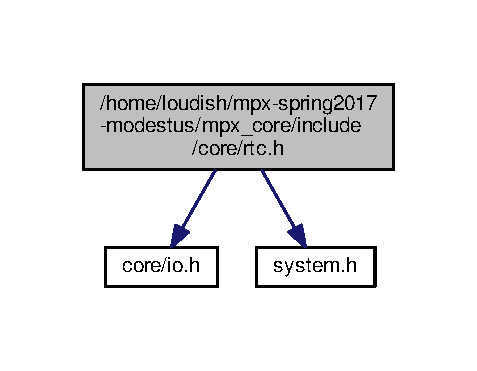
\includegraphics[width=229pt]{rtc_8h__incl}
\end{center}
\end{figure}
This graph shows which files directly or indirectly include this file\+:\nopagebreak
\begin{figure}[H]
\begin{center}
\leavevmode
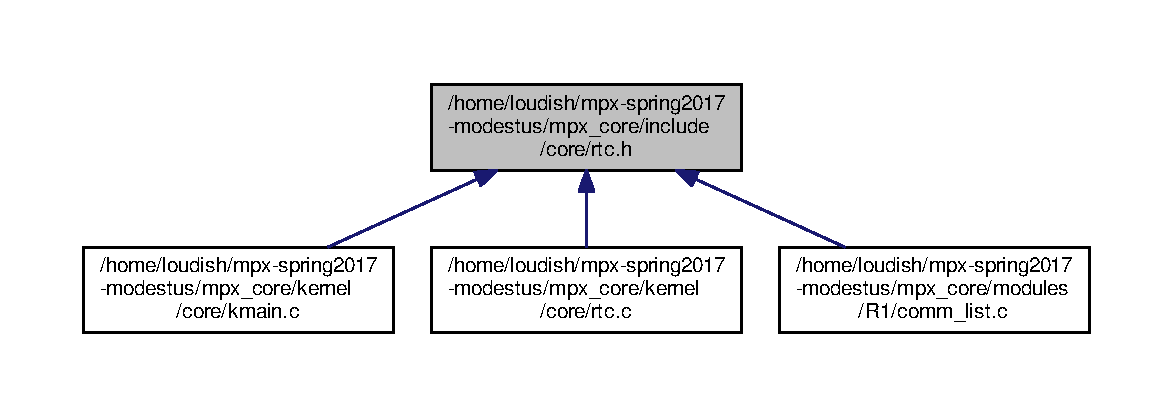
\includegraphics[width=350pt]{rtc_8h__dep__incl}
\end{center}
\end{figure}
\subsection*{Macros}
\begin{DoxyCompactItemize}
\item 
\#define \hyperlink{rtc_8h_a52aed4f0dce6c69eec85228a1fc15e2c}{R\+T\+C\+\_\+\+I\+N\+D\+E\+X\+\_\+\+R\+EG}~0x70
\item 
\#define \hyperlink{rtc_8h_a2f258a00c59c3f347c8d2d4a75471ce0}{R\+T\+C\+\_\+\+D\+A\+T\+A\+\_\+\+R\+EG}~0x71
\item 
\#define \hyperlink{rtc_8h_ad5172920660b0cc3a01124769f769da8}{S\+E\+C\+O\+N\+D\+S\+\_\+\+I\+N\+D\+EX}~0x00
\item 
\#define \hyperlink{rtc_8h_afb7672d6cea1669acd4f76d74ca28459}{M\+I\+N\+U\+T\+E\+S\+\_\+\+I\+N\+D\+EX}~0x02
\item 
\#define \hyperlink{rtc_8h_a58095ff2a9d2a6b458d6ef46fa9d4f68}{H\+O\+U\+R\+S\+\_\+\+I\+N\+D\+EX}~0x04
\item 
\#define \hyperlink{rtc_8h_a3524da1819943d5a94067c1c9e8aa5cc}{D\+A\+Y\+\_\+\+O\+F\+\_\+\+M\+O\+N\+T\+H\+\_\+\+I\+N\+D\+EX}~0x07
\item 
\#define \hyperlink{rtc_8h_a69a2fa993700fb8058ec48611ebbf5c8}{M\+O\+N\+T\+H\+S\+\_\+\+I\+N\+D\+EX}~0x08
\item 
\#define \hyperlink{rtc_8h_a940c790a06a199a1e2136bea0058799e}{Y\+E\+A\+R\+\_\+\+I\+N\+D\+EX}~0x09
\end{DoxyCompactItemize}
\subsection*{Functions}
\begin{DoxyCompactItemize}
\item 
void \hyperlink{rtc_8h_a35fa24488cb7eb077e8dc995729202cf}{get\+\_\+time} (int $\ast$hours, int $\ast$minutes, int $\ast$seconds)
\begin{DoxyCompactList}\small\item\em get\+\_\+time this function will retrieve the system time and place it in three pointers. Military time \end{DoxyCompactList}\item 
void \hyperlink{rtc_8h_a9f75815e4f89e0ff7065999f43867e92}{set\+\_\+time} (int hours, int minutes, int seconds)
\begin{DoxyCompactList}\small\item\em set\+\_\+time sets the R\+TC time. Military time \end{DoxyCompactList}\item 
void \hyperlink{rtc_8h_ab43f56447c49f42bb4baee3e59e2d1f9}{get\+\_\+date} (int $\ast$day, int $\ast$month, int $\ast$year)
\begin{DoxyCompactList}\small\item\em get\+\_\+date this function will retrieve the system date and place in three pointers \end{DoxyCompactList}\item 
void \hyperlink{rtc_8h_a7903b907981d739e3d156a964255d45e}{set\+\_\+date} (int day, int month, int year)
\begin{DoxyCompactList}\small\item\em set\+\_\+date sets the R\+TC Date \end{DoxyCompactList}\end{DoxyCompactItemize}


\subsection{Macro Definition Documentation}
\index{rtc.\+h@{rtc.\+h}!D\+A\+Y\+\_\+\+O\+F\+\_\+\+M\+O\+N\+T\+H\+\_\+\+I\+N\+D\+EX@{D\+A\+Y\+\_\+\+O\+F\+\_\+\+M\+O\+N\+T\+H\+\_\+\+I\+N\+D\+EX}}
\index{D\+A\+Y\+\_\+\+O\+F\+\_\+\+M\+O\+N\+T\+H\+\_\+\+I\+N\+D\+EX@{D\+A\+Y\+\_\+\+O\+F\+\_\+\+M\+O\+N\+T\+H\+\_\+\+I\+N\+D\+EX}!rtc.\+h@{rtc.\+h}}
\subsubsection[{\texorpdfstring{D\+A\+Y\+\_\+\+O\+F\+\_\+\+M\+O\+N\+T\+H\+\_\+\+I\+N\+D\+EX}{DAY_OF_MONTH_INDEX}}]{\setlength{\rightskip}{0pt plus 5cm}\#define D\+A\+Y\+\_\+\+O\+F\+\_\+\+M\+O\+N\+T\+H\+\_\+\+I\+N\+D\+EX~0x07}\hypertarget{rtc_8h_a3524da1819943d5a94067c1c9e8aa5cc}{}\label{rtc_8h_a3524da1819943d5a94067c1c9e8aa5cc}


Definition at line 13 of file rtc.\+h.



Referenced by get\+\_\+date(), and set\+\_\+date().

\index{rtc.\+h@{rtc.\+h}!H\+O\+U\+R\+S\+\_\+\+I\+N\+D\+EX@{H\+O\+U\+R\+S\+\_\+\+I\+N\+D\+EX}}
\index{H\+O\+U\+R\+S\+\_\+\+I\+N\+D\+EX@{H\+O\+U\+R\+S\+\_\+\+I\+N\+D\+EX}!rtc.\+h@{rtc.\+h}}
\subsubsection[{\texorpdfstring{H\+O\+U\+R\+S\+\_\+\+I\+N\+D\+EX}{HOURS_INDEX}}]{\setlength{\rightskip}{0pt plus 5cm}\#define H\+O\+U\+R\+S\+\_\+\+I\+N\+D\+EX~0x04}\hypertarget{rtc_8h_a58095ff2a9d2a6b458d6ef46fa9d4f68}{}\label{rtc_8h_a58095ff2a9d2a6b458d6ef46fa9d4f68}


Definition at line 12 of file rtc.\+h.



Referenced by get\+\_\+time(), and set\+\_\+time().

\index{rtc.\+h@{rtc.\+h}!M\+I\+N\+U\+T\+E\+S\+\_\+\+I\+N\+D\+EX@{M\+I\+N\+U\+T\+E\+S\+\_\+\+I\+N\+D\+EX}}
\index{M\+I\+N\+U\+T\+E\+S\+\_\+\+I\+N\+D\+EX@{M\+I\+N\+U\+T\+E\+S\+\_\+\+I\+N\+D\+EX}!rtc.\+h@{rtc.\+h}}
\subsubsection[{\texorpdfstring{M\+I\+N\+U\+T\+E\+S\+\_\+\+I\+N\+D\+EX}{MINUTES_INDEX}}]{\setlength{\rightskip}{0pt plus 5cm}\#define M\+I\+N\+U\+T\+E\+S\+\_\+\+I\+N\+D\+EX~0x02}\hypertarget{rtc_8h_afb7672d6cea1669acd4f76d74ca28459}{}\label{rtc_8h_afb7672d6cea1669acd4f76d74ca28459}


Definition at line 11 of file rtc.\+h.



Referenced by get\+\_\+time(), and set\+\_\+time().

\index{rtc.\+h@{rtc.\+h}!M\+O\+N\+T\+H\+S\+\_\+\+I\+N\+D\+EX@{M\+O\+N\+T\+H\+S\+\_\+\+I\+N\+D\+EX}}
\index{M\+O\+N\+T\+H\+S\+\_\+\+I\+N\+D\+EX@{M\+O\+N\+T\+H\+S\+\_\+\+I\+N\+D\+EX}!rtc.\+h@{rtc.\+h}}
\subsubsection[{\texorpdfstring{M\+O\+N\+T\+H\+S\+\_\+\+I\+N\+D\+EX}{MONTHS_INDEX}}]{\setlength{\rightskip}{0pt plus 5cm}\#define M\+O\+N\+T\+H\+S\+\_\+\+I\+N\+D\+EX~0x08}\hypertarget{rtc_8h_a69a2fa993700fb8058ec48611ebbf5c8}{}\label{rtc_8h_a69a2fa993700fb8058ec48611ebbf5c8}


Definition at line 14 of file rtc.\+h.



Referenced by get\+\_\+date(), and set\+\_\+date().

\index{rtc.\+h@{rtc.\+h}!R\+T\+C\+\_\+\+D\+A\+T\+A\+\_\+\+R\+EG@{R\+T\+C\+\_\+\+D\+A\+T\+A\+\_\+\+R\+EG}}
\index{R\+T\+C\+\_\+\+D\+A\+T\+A\+\_\+\+R\+EG@{R\+T\+C\+\_\+\+D\+A\+T\+A\+\_\+\+R\+EG}!rtc.\+h@{rtc.\+h}}
\subsubsection[{\texorpdfstring{R\+T\+C\+\_\+\+D\+A\+T\+A\+\_\+\+R\+EG}{RTC_DATA_REG}}]{\setlength{\rightskip}{0pt plus 5cm}\#define R\+T\+C\+\_\+\+D\+A\+T\+A\+\_\+\+R\+EG~0x71}\hypertarget{rtc_8h_a2f258a00c59c3f347c8d2d4a75471ce0}{}\label{rtc_8h_a2f258a00c59c3f347c8d2d4a75471ce0}


Definition at line 8 of file rtc.\+h.



Referenced by set\+\_\+date(), and set\+\_\+time().

\index{rtc.\+h@{rtc.\+h}!R\+T\+C\+\_\+\+I\+N\+D\+E\+X\+\_\+\+R\+EG@{R\+T\+C\+\_\+\+I\+N\+D\+E\+X\+\_\+\+R\+EG}}
\index{R\+T\+C\+\_\+\+I\+N\+D\+E\+X\+\_\+\+R\+EG@{R\+T\+C\+\_\+\+I\+N\+D\+E\+X\+\_\+\+R\+EG}!rtc.\+h@{rtc.\+h}}
\subsubsection[{\texorpdfstring{R\+T\+C\+\_\+\+I\+N\+D\+E\+X\+\_\+\+R\+EG}{RTC_INDEX_REG}}]{\setlength{\rightskip}{0pt plus 5cm}\#define R\+T\+C\+\_\+\+I\+N\+D\+E\+X\+\_\+\+R\+EG~0x70}\hypertarget{rtc_8h_a52aed4f0dce6c69eec85228a1fc15e2c}{}\label{rtc_8h_a52aed4f0dce6c69eec85228a1fc15e2c}


Definition at line 7 of file rtc.\+h.



Referenced by get\+\_\+date(), get\+\_\+time(), set\+\_\+date(), and set\+\_\+time().

\index{rtc.\+h@{rtc.\+h}!S\+E\+C\+O\+N\+D\+S\+\_\+\+I\+N\+D\+EX@{S\+E\+C\+O\+N\+D\+S\+\_\+\+I\+N\+D\+EX}}
\index{S\+E\+C\+O\+N\+D\+S\+\_\+\+I\+N\+D\+EX@{S\+E\+C\+O\+N\+D\+S\+\_\+\+I\+N\+D\+EX}!rtc.\+h@{rtc.\+h}}
\subsubsection[{\texorpdfstring{S\+E\+C\+O\+N\+D\+S\+\_\+\+I\+N\+D\+EX}{SECONDS_INDEX}}]{\setlength{\rightskip}{0pt plus 5cm}\#define S\+E\+C\+O\+N\+D\+S\+\_\+\+I\+N\+D\+EX~0x00}\hypertarget{rtc_8h_ad5172920660b0cc3a01124769f769da8}{}\label{rtc_8h_ad5172920660b0cc3a01124769f769da8}


Definition at line 10 of file rtc.\+h.



Referenced by get\+\_\+time(), and set\+\_\+time().

\index{rtc.\+h@{rtc.\+h}!Y\+E\+A\+R\+\_\+\+I\+N\+D\+EX@{Y\+E\+A\+R\+\_\+\+I\+N\+D\+EX}}
\index{Y\+E\+A\+R\+\_\+\+I\+N\+D\+EX@{Y\+E\+A\+R\+\_\+\+I\+N\+D\+EX}!rtc.\+h@{rtc.\+h}}
\subsubsection[{\texorpdfstring{Y\+E\+A\+R\+\_\+\+I\+N\+D\+EX}{YEAR_INDEX}}]{\setlength{\rightskip}{0pt plus 5cm}\#define Y\+E\+A\+R\+\_\+\+I\+N\+D\+EX~0x09}\hypertarget{rtc_8h_a940c790a06a199a1e2136bea0058799e}{}\label{rtc_8h_a940c790a06a199a1e2136bea0058799e}


Definition at line 15 of file rtc.\+h.



Referenced by get\+\_\+date(), and set\+\_\+date().



\subsection{Function Documentation}
\index{rtc.\+h@{rtc.\+h}!get\+\_\+date@{get\+\_\+date}}
\index{get\+\_\+date@{get\+\_\+date}!rtc.\+h@{rtc.\+h}}
\subsubsection[{\texorpdfstring{get\+\_\+date(int $\ast$day, int $\ast$month, int $\ast$year)}{get_date(int *day, int *month, int *year)}}]{\setlength{\rightskip}{0pt plus 5cm}void get\+\_\+date (
\begin{DoxyParamCaption}
\item[{int $\ast$}]{day, }
\item[{int $\ast$}]{month, }
\item[{int $\ast$}]{year}
\end{DoxyParamCaption}
)}\hypertarget{rtc_8h_ab43f56447c49f42bb4baee3e59e2d1f9}{}\label{rtc_8h_ab43f56447c49f42bb4baee3e59e2d1f9}


get\+\_\+date this function will retrieve the system date and place in three pointers 


\begin{DoxyParams}{Parameters}
{\em day} & pointer to int where the current day will be stored, U\+TC Time zone \\
\hline
{\em months} & pointer to int where the current month will be stored, U\+TC Time zone \\
\hline
{\em year} & pointer to int where the current year will be stored, U\+TC Time zone \\
\hline
\end{DoxyParams}


Definition at line 56 of file rtc.\+c.



References D\+A\+Y\+\_\+\+O\+F\+\_\+\+M\+O\+N\+T\+H\+\_\+\+I\+N\+D\+EX, inb, M\+O\+N\+T\+H\+S\+\_\+\+I\+N\+D\+EX, outb, R\+T\+C\+\_\+\+I\+N\+D\+E\+X\+\_\+\+R\+EG, and Y\+E\+A\+R\+\_\+\+I\+N\+D\+EX.



Referenced by get\+Date(), and kmain().


\begin{DoxyCode}
57 \{
58     \textcolor{keywordtype}{char} temp = 0;
59     \hyperlink{io_8h_a0e661d36f40638a36550a534076f155b}{outb}(\hyperlink{rtc_8h_a52aed4f0dce6c69eec85228a1fc15e2c}{RTC\_INDEX\_REG}, \hyperlink{rtc_8h_a3524da1819943d5a94067c1c9e8aa5cc}{DAY\_OF\_MONTH\_INDEX});
60     temp = \hyperlink{io_8h_ad6488a48837d179b1833e2f48dac9665}{inb}(0x71);
61     *day = ((temp & 0xf0) >>4 ) *10 + (temp & 0x0f);
62 
63     \hyperlink{io_8h_a0e661d36f40638a36550a534076f155b}{outb}(\hyperlink{rtc_8h_a52aed4f0dce6c69eec85228a1fc15e2c}{RTC\_INDEX\_REG}, \hyperlink{rtc_8h_a69a2fa993700fb8058ec48611ebbf5c8}{MONTHS\_INDEX});
64     temp = \hyperlink{io_8h_ad6488a48837d179b1833e2f48dac9665}{inb}(0x71);
65     *month = ((temp & 0xf0) >>4 ) *10 + (temp & 0x0f);
66 
67     \hyperlink{io_8h_a0e661d36f40638a36550a534076f155b}{outb}(\hyperlink{rtc_8h_a52aed4f0dce6c69eec85228a1fc15e2c}{RTC\_INDEX\_REG}, \hyperlink{rtc_8h_a940c790a06a199a1e2136bea0058799e}{YEAR\_INDEX});
68     temp = \hyperlink{io_8h_ad6488a48837d179b1833e2f48dac9665}{inb}(0x71);
69     *year = ((temp & 0xf0) >>4 ) *10 + (temp & 0x0f);
70 \}
\end{DoxyCode}
\index{rtc.\+h@{rtc.\+h}!get\+\_\+time@{get\+\_\+time}}
\index{get\+\_\+time@{get\+\_\+time}!rtc.\+h@{rtc.\+h}}
\subsubsection[{\texorpdfstring{get\+\_\+time(int $\ast$hours, int $\ast$minutes, int $\ast$seconds)}{get_time(int *hours, int *minutes, int *seconds)}}]{\setlength{\rightskip}{0pt plus 5cm}void get\+\_\+time (
\begin{DoxyParamCaption}
\item[{int $\ast$}]{hours, }
\item[{int $\ast$}]{minutes, }
\item[{int $\ast$}]{seconds}
\end{DoxyParamCaption}
)}\hypertarget{rtc_8h_a35fa24488cb7eb077e8dc995729202cf}{}\label{rtc_8h_a35fa24488cb7eb077e8dc995729202cf}


get\+\_\+time this function will retrieve the system time and place it in three pointers. Military time 


\begin{DoxyParams}{Parameters}
{\em hours} & pointer to int where the current hours will be stored, in U\+TC timezone \\
\hline
{\em minutes} & pointer to int where the current minutes will be stored, in U\+TC timezone \\
\hline
{\em seconds} & pointer to int where the current seconds will be stored, in U\+TC timezone\\
\hline
\end{DoxyParams}
get\+\_\+time this function will retrieve the system time and place it in three pointers. Military time


\begin{DoxyParams}{Parameters}
{\em hours} & pointer to int where the current hours will be stored, in U\+TC timezone \\
\hline
{\em minutes} & pointer to int where the current minutes will be stored, in U\+TC timezone \\
\hline
{\em seconds} & pointer to int where the current seconds will be stored, in U\+TC timezone \\
\hline
\end{DoxyParams}


Definition at line 10 of file rtc.\+c.



References H\+O\+U\+R\+S\+\_\+\+I\+N\+D\+EX, inb, M\+I\+N\+U\+T\+E\+S\+\_\+\+I\+N\+D\+EX, outb, R\+T\+C\+\_\+\+I\+N\+D\+E\+X\+\_\+\+R\+EG, and S\+E\+C\+O\+N\+D\+S\+\_\+\+I\+N\+D\+EX.



Referenced by get\+Time(), and kmain().


\begin{DoxyCode}
11 \{
12     \textcolor{keywordtype}{char} temp = 0;
13     \hyperlink{io_8h_a0e661d36f40638a36550a534076f155b}{outb}(\hyperlink{rtc_8h_a52aed4f0dce6c69eec85228a1fc15e2c}{RTC\_INDEX\_REG}, \hyperlink{rtc_8h_ad5172920660b0cc3a01124769f769da8}{SECONDS\_INDEX});
14     temp = \hyperlink{io_8h_ad6488a48837d179b1833e2f48dac9665}{inb}(0x71);
15     *seconds = ((temp & 0xf0) >>4 ) *10 + (temp & 0x0f);
16 
17     \hyperlink{io_8h_a0e661d36f40638a36550a534076f155b}{outb}(\hyperlink{rtc_8h_a52aed4f0dce6c69eec85228a1fc15e2c}{RTC\_INDEX\_REG}, \hyperlink{rtc_8h_afb7672d6cea1669acd4f76d74ca28459}{MINUTES\_INDEX});
18     temp = \hyperlink{io_8h_ad6488a48837d179b1833e2f48dac9665}{inb}(0x71);
19     *minutes = ((temp & 0xf0) >>4 ) *10 + (temp & 0x0f);
20 
21     \hyperlink{io_8h_a0e661d36f40638a36550a534076f155b}{outb}(\hyperlink{rtc_8h_a52aed4f0dce6c69eec85228a1fc15e2c}{RTC\_INDEX\_REG}, \hyperlink{rtc_8h_a58095ff2a9d2a6b458d6ef46fa9d4f68}{HOURS\_INDEX});
22     temp = \hyperlink{io_8h_ad6488a48837d179b1833e2f48dac9665}{inb}(0x71);
23     *hours = ((temp & 0xf0) >>4 ) *10 + (temp & 0x0f);
24 \}
\end{DoxyCode}
\index{rtc.\+h@{rtc.\+h}!set\+\_\+date@{set\+\_\+date}}
\index{set\+\_\+date@{set\+\_\+date}!rtc.\+h@{rtc.\+h}}
\subsubsection[{\texorpdfstring{set\+\_\+date(int day, int month, int year)}{set_date(int day, int month, int year)}}]{\setlength{\rightskip}{0pt plus 5cm}void set\+\_\+date (
\begin{DoxyParamCaption}
\item[{int}]{day, }
\item[{int}]{month, }
\item[{int}]{year}
\end{DoxyParamCaption}
)}\hypertarget{rtc_8h_a7903b907981d739e3d156a964255d45e}{}\label{rtc_8h_a7903b907981d739e3d156a964255d45e}


set\+\_\+date sets the R\+TC Date 


\begin{DoxyParams}{Parameters}
{\em day} & the day to set the clock to, must be valid for the month. U\+TC Time zone \\
\hline
{\em month} & the month to set the clock to, must be between 1 and 12. U\+TC Time zone \\
\hline
{\em year} & the year to set the clock to, must be less than 100. U\+TC Time zone \\
\hline
\end{DoxyParams}


Definition at line 79 of file rtc.\+c.



References cli, D\+A\+Y\+\_\+\+O\+F\+\_\+\+M\+O\+N\+T\+H\+\_\+\+I\+N\+D\+EX, M\+O\+N\+T\+H\+S\+\_\+\+I\+N\+D\+EX, outb, R\+T\+C\+\_\+\+D\+A\+T\+A\+\_\+\+R\+EG, R\+T\+C\+\_\+\+I\+N\+D\+E\+X\+\_\+\+R\+EG, sti, and Y\+E\+A\+R\+\_\+\+I\+N\+D\+EX.



Referenced by set\+Date().


\begin{DoxyCode}
80 \{
81     \hyperlink{system_8h_ac5d15f274bc9b1e96230f3d3c60fd1f8}{sti}();
82 
83     \hyperlink{io_8h_a0e661d36f40638a36550a534076f155b}{outb}(\hyperlink{rtc_8h_a52aed4f0dce6c69eec85228a1fc15e2c}{RTC\_INDEX\_REG}, \hyperlink{rtc_8h_a3524da1819943d5a94067c1c9e8aa5cc}{DAY\_OF\_MONTH\_INDEX});
84     \hyperlink{io_8h_a0e661d36f40638a36550a534076f155b}{outb}(\hyperlink{rtc_8h_a2f258a00c59c3f347c8d2d4a75471ce0}{RTC\_DATA\_REG}, ((day/10)<<4)|(day%10));
85 
86     \hyperlink{io_8h_a0e661d36f40638a36550a534076f155b}{outb}(\hyperlink{rtc_8h_a52aed4f0dce6c69eec85228a1fc15e2c}{RTC\_INDEX\_REG}, \hyperlink{rtc_8h_a69a2fa993700fb8058ec48611ebbf5c8}{MONTHS\_INDEX});
87     \hyperlink{io_8h_a0e661d36f40638a36550a534076f155b}{outb}(\hyperlink{rtc_8h_a2f258a00c59c3f347c8d2d4a75471ce0}{RTC\_DATA\_REG}, ((month/10)<<4)|(month%10));
88 
89     \hyperlink{io_8h_a0e661d36f40638a36550a534076f155b}{outb}(\hyperlink{rtc_8h_a52aed4f0dce6c69eec85228a1fc15e2c}{RTC\_INDEX\_REG}, \hyperlink{rtc_8h_a940c790a06a199a1e2136bea0058799e}{YEAR\_INDEX});
90     \hyperlink{io_8h_a0e661d36f40638a36550a534076f155b}{outb}(\hyperlink{rtc_8h_a2f258a00c59c3f347c8d2d4a75471ce0}{RTC\_DATA\_REG}, (((year-(year/100)*100)/10)<<4)|(year%10) );
91 
92     \hyperlink{system_8h_a68c330e94fe121eba993e5a5973c3162}{cli}();
93 \}
\end{DoxyCode}
\index{rtc.\+h@{rtc.\+h}!set\+\_\+time@{set\+\_\+time}}
\index{set\+\_\+time@{set\+\_\+time}!rtc.\+h@{rtc.\+h}}
\subsubsection[{\texorpdfstring{set\+\_\+time(int hours, int minutes, int seconds)}{set_time(int hours, int minutes, int seconds)}}]{\setlength{\rightskip}{0pt plus 5cm}void set\+\_\+time (
\begin{DoxyParamCaption}
\item[{int}]{hours, }
\item[{int}]{minutes, }
\item[{int}]{seconds}
\end{DoxyParamCaption}
)}\hypertarget{rtc_8h_a9f75815e4f89e0ff7065999f43867e92}{}\label{rtc_8h_a9f75815e4f89e0ff7065999f43867e92}


set\+\_\+time sets the R\+TC time. Military time 


\begin{DoxyParams}{Parameters}
{\em hours} & the hours to set the clock to, must be less than 24. In U\+TC Time zone \\
\hline
{\em minutes} & the minutes to set the clock to, must be less than 60. In U\+TC Time zone \\
\hline
{\em seconds} & the seconds to set the clock to, must be less than 60. In U\+TC Time zone\\
\hline
\end{DoxyParams}
set\+\_\+time sets the R\+TC time. Military time


\begin{DoxyParams}{Parameters}
{\em hours} & the hours to set the clock to, must be less than 24. In U\+TC Time zone \\
\hline
{\em minutes} & the minutes to set the clock to, must be less than 60. In U\+TC Time zone \\
\hline
{\em seconds} & the seconds to set the clock to, must be less than 60. In U\+TC Time zone \\
\hline
\end{DoxyParams}


Definition at line 33 of file rtc.\+c.



References cli, H\+O\+U\+R\+S\+\_\+\+I\+N\+D\+EX, M\+I\+N\+U\+T\+E\+S\+\_\+\+I\+N\+D\+EX, outb, R\+T\+C\+\_\+\+D\+A\+T\+A\+\_\+\+R\+EG, R\+T\+C\+\_\+\+I\+N\+D\+E\+X\+\_\+\+R\+EG, S\+E\+C\+O\+N\+D\+S\+\_\+\+I\+N\+D\+EX, and sti.



Referenced by set\+Time().


\begin{DoxyCode}
34 \{
35     \hyperlink{system_8h_ac5d15f274bc9b1e96230f3d3c60fd1f8}{sti}();
36 
37     \hyperlink{io_8h_a0e661d36f40638a36550a534076f155b}{outb}(\hyperlink{rtc_8h_a52aed4f0dce6c69eec85228a1fc15e2c}{RTC\_INDEX\_REG}, \hyperlink{rtc_8h_a58095ff2a9d2a6b458d6ef46fa9d4f68}{HOURS\_INDEX});
38     \hyperlink{io_8h_a0e661d36f40638a36550a534076f155b}{outb}(\hyperlink{rtc_8h_a2f258a00c59c3f347c8d2d4a75471ce0}{RTC\_DATA\_REG}, ((hours/10)<<4)|(hours%10) );
39 
40     \hyperlink{io_8h_a0e661d36f40638a36550a534076f155b}{outb}(\hyperlink{rtc_8h_a52aed4f0dce6c69eec85228a1fc15e2c}{RTC\_INDEX\_REG}, \hyperlink{rtc_8h_afb7672d6cea1669acd4f76d74ca28459}{MINUTES\_INDEX});
41     \hyperlink{io_8h_a0e661d36f40638a36550a534076f155b}{outb}(\hyperlink{rtc_8h_a2f258a00c59c3f347c8d2d4a75471ce0}{RTC\_DATA\_REG}, ((minutes/10)<<4)|(minutes%10) );
42 
43     \hyperlink{io_8h_a0e661d36f40638a36550a534076f155b}{outb}(\hyperlink{rtc_8h_a52aed4f0dce6c69eec85228a1fc15e2c}{RTC\_INDEX\_REG}, \hyperlink{rtc_8h_ad5172920660b0cc3a01124769f769da8}{SECONDS\_INDEX});
44     \hyperlink{io_8h_a0e661d36f40638a36550a534076f155b}{outb}(\hyperlink{rtc_8h_a2f258a00c59c3f347c8d2d4a75471ce0}{RTC\_DATA\_REG}, ((seconds/10)<<4)|(seconds%10) );
45 
46     \hyperlink{system_8h_a68c330e94fe121eba993e5a5973c3162}{cli}();
47 \}
\end{DoxyCode}

\hypertarget{serial_8h}{}\section{/home/loudish/mpx-\/spring2017-\/modestus/mpx\+\_\+core/include/core/serial.h File Reference}
\label{serial_8h}\index{/home/loudish/mpx-\/spring2017-\/modestus/mpx\+\_\+core/include/core/serial.\+h@{/home/loudish/mpx-\/spring2017-\/modestus/mpx\+\_\+core/include/core/serial.\+h}}
{\ttfamily \#include $<$input.\+h$>$}\\*
Include dependency graph for serial.\+h\+:\nopagebreak
\begin{figure}[H]
\begin{center}
\leavevmode
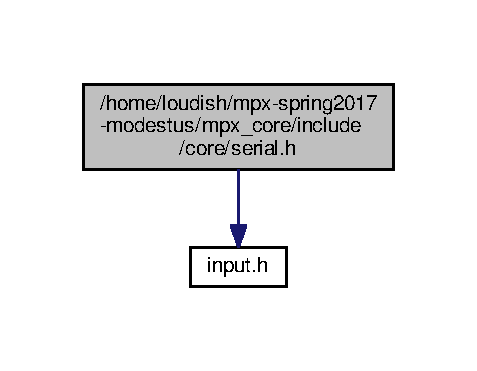
\includegraphics[width=229pt]{serial_8h__incl}
\end{center}
\end{figure}
This graph shows which files directly or indirectly include this file\+:\nopagebreak
\begin{figure}[H]
\begin{center}
\leavevmode
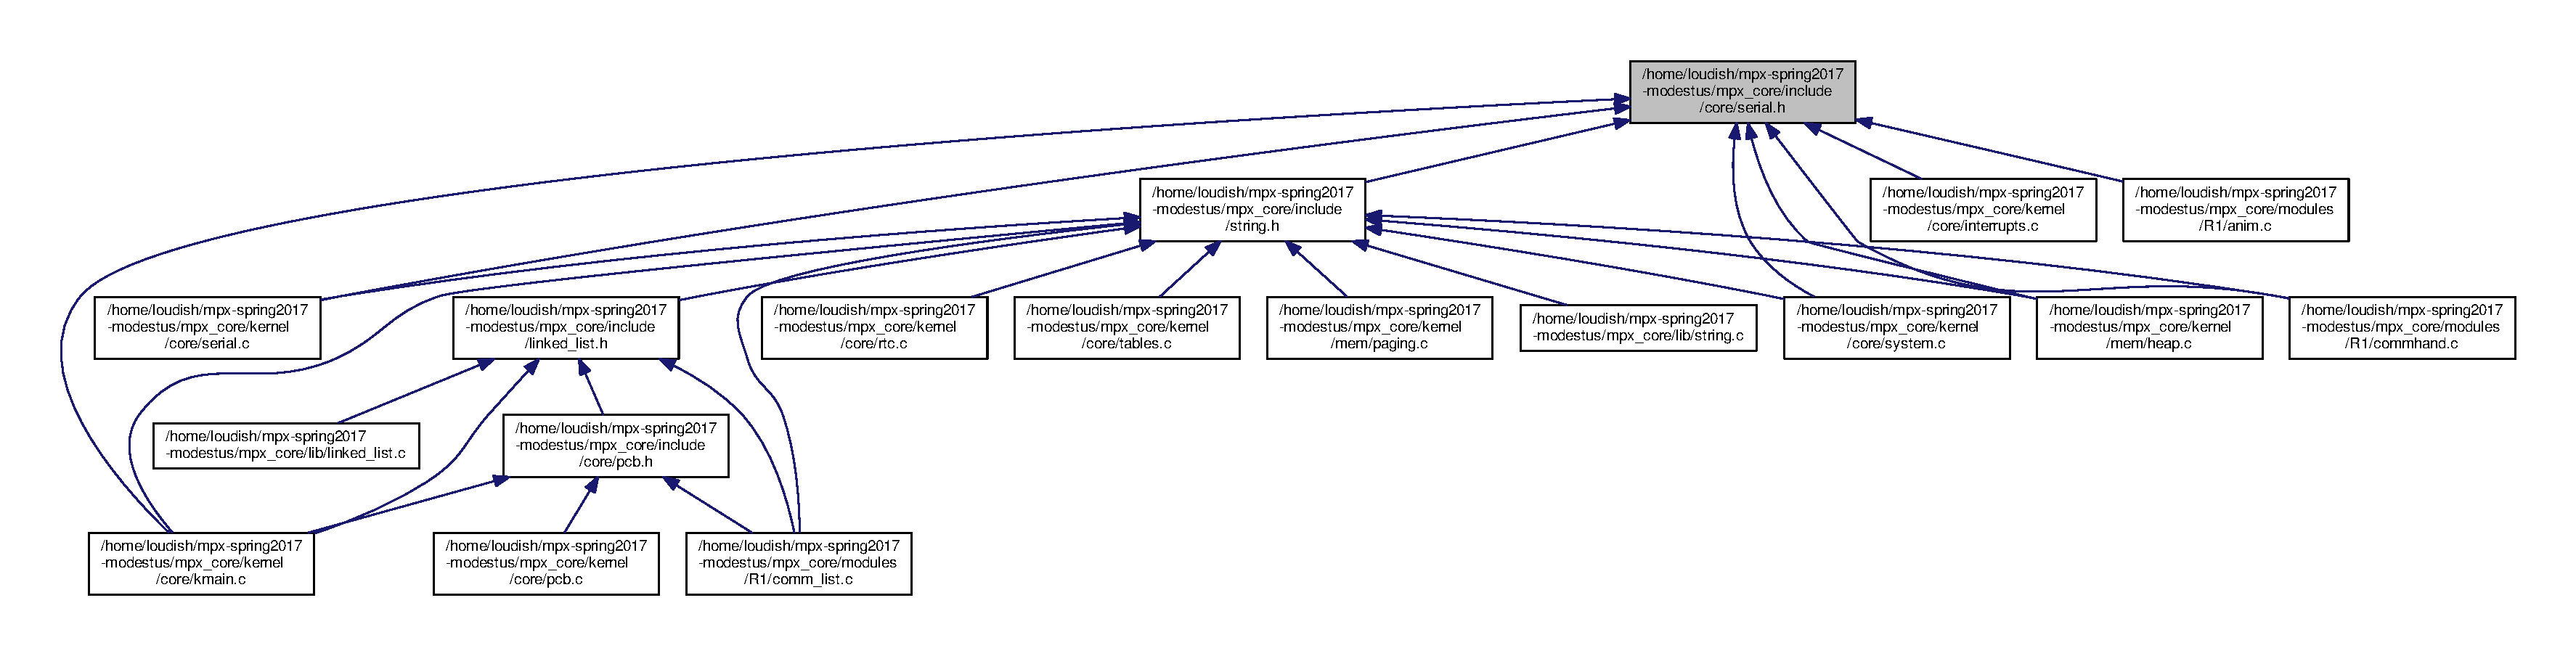
\includegraphics[width=350pt]{serial_8h__dep__incl}
\end{center}
\end{figure}
\subsection*{Macros}
\begin{DoxyCompactItemize}
\item 
\#define \hyperlink{serial_8h_a00dbb3ab1c59e14699be9393693e2248}{C\+O\+M1}~0x3f8
\item 
\#define \hyperlink{serial_8h_a435e02f194c24c9b0e00d7cd27a1704e}{C\+O\+M2}~0x2f8
\item 
\#define \hyperlink{serial_8h_abbed02672431595364c5dd35809303a6}{C\+O\+M3}~0x3e8
\item 
\#define \hyperlink{serial_8h_a595cabb01568ba641574d24546d99c6b}{C\+O\+M4}~0x2e8
\end{DoxyCompactItemize}
\subsection*{Functions}
\begin{DoxyCompactItemize}
\item 
int \hyperlink{serial_8h_a7078c07ff8b2c48780558549a8f7cf90}{init\+\_\+serial} (int device)
\item 
int \hyperlink{serial_8h_a3514f7abff236a4e00a6c46021ce5e22}{serial\+\_\+println} (const char $\ast$msg)
\item 
int \hyperlink{serial_8h_a995827efcd4dcfb780c9fbb9645410a4}{serial\+\_\+print} (const char $\ast$msg)
\item 
int \hyperlink{serial_8h_ae97b87ee1f57c687e7fca6f9958e03ef}{set\+\_\+serial\+\_\+out} (int device)
\item 
int \hyperlink{serial_8h_a3f4008da5feabfb7e086f6673a81104b}{set\+\_\+serial\+\_\+in} (int device)
\item 
char $\ast$ \hyperlink{serial_8h_a4b7cdfe478986c0d41a54f2c4a683136}{serial\+\_\+poll} (char \hyperlink{commhand_8c_a304f731e770f19e932c39d189c8cb56f}{in\+\_\+string}\mbox{[}\hyperlink{input_8h_a7a9a231e30b47bc0345749c8bd1e5077}{M\+A\+X\+\_\+\+L\+E\+N\+G\+TH}\mbox{]})
\end{DoxyCompactItemize}


\subsection{Macro Definition Documentation}
\index{serial.\+h@{serial.\+h}!C\+O\+M1@{C\+O\+M1}}
\index{C\+O\+M1@{C\+O\+M1}!serial.\+h@{serial.\+h}}
\subsubsection[{\texorpdfstring{C\+O\+M1}{COM1}}]{\setlength{\rightskip}{0pt plus 5cm}\#define C\+O\+M1~0x3f8}\hypertarget{serial_8h_a00dbb3ab1c59e14699be9393693e2248}{}\label{serial_8h_a00dbb3ab1c59e14699be9393693e2248}


Definition at line 6 of file serial.\+h.



Referenced by kmain(), and serial\+\_\+poll().

\index{serial.\+h@{serial.\+h}!C\+O\+M2@{C\+O\+M2}}
\index{C\+O\+M2@{C\+O\+M2}!serial.\+h@{serial.\+h}}
\subsubsection[{\texorpdfstring{C\+O\+M2}{COM2}}]{\setlength{\rightskip}{0pt plus 5cm}\#define C\+O\+M2~0x2f8}\hypertarget{serial_8h_a435e02f194c24c9b0e00d7cd27a1704e}{}\label{serial_8h_a435e02f194c24c9b0e00d7cd27a1704e}


Definition at line 7 of file serial.\+h.



Referenced by do\+\_\+isr().

\index{serial.\+h@{serial.\+h}!C\+O\+M3@{C\+O\+M3}}
\index{C\+O\+M3@{C\+O\+M3}!serial.\+h@{serial.\+h}}
\subsubsection[{\texorpdfstring{C\+O\+M3}{COM3}}]{\setlength{\rightskip}{0pt plus 5cm}\#define C\+O\+M3~0x3e8}\hypertarget{serial_8h_abbed02672431595364c5dd35809303a6}{}\label{serial_8h_abbed02672431595364c5dd35809303a6}


Definition at line 8 of file serial.\+h.

\index{serial.\+h@{serial.\+h}!C\+O\+M4@{C\+O\+M4}}
\index{C\+O\+M4@{C\+O\+M4}!serial.\+h@{serial.\+h}}
\subsubsection[{\texorpdfstring{C\+O\+M4}{COM4}}]{\setlength{\rightskip}{0pt plus 5cm}\#define C\+O\+M4~0x2e8}\hypertarget{serial_8h_a595cabb01568ba641574d24546d99c6b}{}\label{serial_8h_a595cabb01568ba641574d24546d99c6b}


Definition at line 9 of file serial.\+h.



\subsection{Function Documentation}
\index{serial.\+h@{serial.\+h}!init\+\_\+serial@{init\+\_\+serial}}
\index{init\+\_\+serial@{init\+\_\+serial}!serial.\+h@{serial.\+h}}
\subsubsection[{\texorpdfstring{init\+\_\+serial(int device)}{init_serial(int device)}}]{\setlength{\rightskip}{0pt plus 5cm}int init\+\_\+serial (
\begin{DoxyParamCaption}
\item[{int}]{device}
\end{DoxyParamCaption}
)}\hypertarget{serial_8h_a7078c07ff8b2c48780558549a8f7cf90}{}\label{serial_8h_a7078c07ff8b2c48780558549a8f7cf90}


Definition at line 26 of file serial.\+c.



References inb, N\+O\+\_\+\+E\+R\+R\+OR, and outb.


\begin{DoxyCode}
27 \{
28   \hyperlink{io_8h_a0e661d36f40638a36550a534076f155b}{outb}(device + 1, 0x00); \textcolor{comment}{//disable interrupts}
29   \hyperlink{io_8h_a0e661d36f40638a36550a534076f155b}{outb}(device + 3, 0x80); \textcolor{comment}{//set line control register}
30   \hyperlink{io_8h_a0e661d36f40638a36550a534076f155b}{outb}(device + 0, 115200/9600); \textcolor{comment}{//set bsd least sig bit}
31   \hyperlink{io_8h_a0e661d36f40638a36550a534076f155b}{outb}(device + 1, 0x00); \textcolor{comment}{//brd most significant bit}
32   \hyperlink{io_8h_a0e661d36f40638a36550a534076f155b}{outb}(device + 3, 0x03); \textcolor{comment}{//lock divisor; 8bits, no parity, one stop}
33   \hyperlink{io_8h_a0e661d36f40638a36550a534076f155b}{outb}(device + 2, 0xC7); \textcolor{comment}{//enable fifo, clear, 14byte threshold}
34   \hyperlink{io_8h_a0e661d36f40638a36550a534076f155b}{outb}(device + 4, 0x0B); \textcolor{comment}{//enable interrupts, rts/dsr set}
35   (void)\hyperlink{io_8h_ad6488a48837d179b1833e2f48dac9665}{inb}(device);      \textcolor{comment}{//read bit to reset port}
36   \textcolor{keywordflow}{return} \hyperlink{serial_8c_a258bb72419ef143530a2f8f55e7d57af}{NO\_ERROR};
37 \}
\end{DoxyCode}
\index{serial.\+h@{serial.\+h}!serial\+\_\+poll@{serial\+\_\+poll}}
\index{serial\+\_\+poll@{serial\+\_\+poll}!serial.\+h@{serial.\+h}}
\subsubsection[{\texorpdfstring{serial\+\_\+poll(char in\+\_\+string[M\+A\+X\+\_\+\+L\+E\+N\+G\+TH])}{serial_poll(char in_string[MAX_LENGTH])}}]{\setlength{\rightskip}{0pt plus 5cm}char$\ast$ serial\+\_\+poll (
\begin{DoxyParamCaption}
\item[{char}]{in\+\_\+string\mbox{[}\+M\+A\+X\+\_\+\+L\+E\+N\+G\+T\+H\mbox{]}}
\end{DoxyParamCaption}
)}\hypertarget{serial_8h_a4b7cdfe478986c0d41a54f2c4a683136}{}\label{serial_8h_a4b7cdfe478986c0d41a54f2c4a683136}


Definition at line 114 of file serial.\+c.



References B\+A\+C\+K\+S\+P\+A\+CE, clear\+\_\+buff(), C\+O\+M1, D\+E\+L\+E\+TE, E\+SC, in\+\_\+string, inb, N\+E\+W\+\_\+\+L\+I\+NE, R\+E\+T\+U\+RN, return\+\_\+cursor(), serial\+\_\+print(), and strcpy().



Referenced by init\+\_\+commhand().


\begin{DoxyCode}
114                                               \{
115     \textcolor{comment}{//in\_char is the character read from the register}
116     \textcolor{comment}{//out\_char is that character with a null terminator appended on the end}
117     \textcolor{comment}{//length is the current size of the input}
118     \textcolor{comment}{//cursor\_loc is the current location of the cursor in the input}
119     \textcolor{keywordtype}{char} in\_char;
120     \textcolor{keywordtype}{char} out\_char[2];
121     out\_char[1] = \textcolor{charliteral}{'\(\backslash\)0'};
122     \textcolor{keywordtype}{int} length = 0;
123     \textcolor{keywordtype}{int} cursor\_loc = 0;
124 
125     \textcolor{comment}{//polling for user input}
126     \textcolor{keywordflow}{while} (1) \{
127 
128         \textcolor{keywordflow}{if} (\hyperlink{io_8h_ad6488a48837d179b1833e2f48dac9665}{inb}(\hyperlink{serial_8h_a00dbb3ab1c59e14699be9393693e2248}{COM1}+5)&1) \{
129             \textcolor{comment}{//the character is read from the register}
130             in\_char = \hyperlink{io_8h_ad6488a48837d179b1833e2f48dac9665}{inb}(\hyperlink{serial_8h_a00dbb3ab1c59e14699be9393693e2248}{COM1});
131             out\_char[0] = in\_char;
132 
133             \textcolor{keywordflow}{if} (in\_char == \hyperlink{input_8h_a629568514359445d2fbda71d70eeb1ce}{BACKSPACE}) \{
134                 \textcolor{keywordflow}{if} (length != 0) \{
135                     \textcolor{keywordflow}{if} (cursor\_loc == length)
136                     \{
137                         cursor\_loc--;
138                         \hyperlink{commhand_8c_a304f731e770f19e932c39d189c8cb56f}{in\_string}[cursor\_loc] = \textcolor{charliteral}{'\(\backslash\)0'};
139                         \hyperlink{serial_8c_a337da5154672f3b359cf70d7b78f0c0d}{clear\_buff}();
140                         \hyperlink{serial_8c_a995827efcd4dcfb780c9fbb9645410a4}{serial\_print}(\hyperlink{commhand_8c_a304f731e770f19e932c39d189c8cb56f}{in\_string});
141                         length--;
142                         \hyperlink{serial_8c_a8f0293a95ba79d7dafe198c2cb75549f}{return\_cursor}(cursor\_loc, length);
143 
144                     \}
145                     \textcolor{keywordflow}{else}
146                     \{
147                         cursor\_loc--;
148                         \hyperlink{string_8h_a1eb9cae61e6a6282c28dbc298ef7297e}{strcpy}(&\hyperlink{commhand_8c_a304f731e770f19e932c39d189c8cb56f}{in\_string}[cursor\_loc], &\hyperlink{commhand_8c_a304f731e770f19e932c39d189c8cb56f}{in\_string}[cursor\_loc + 1]);
149                         \hyperlink{commhand_8c_a304f731e770f19e932c39d189c8cb56f}{in\_string}[length - 1] = \textcolor{charliteral}{'\(\backslash\)0'};
150                         \hyperlink{serial_8c_a337da5154672f3b359cf70d7b78f0c0d}{clear\_buff}();
151                         \hyperlink{serial_8c_a995827efcd4dcfb780c9fbb9645410a4}{serial\_print}(\hyperlink{commhand_8c_a304f731e770f19e932c39d189c8cb56f}{in\_string});
152                         length--;
153                         \hyperlink{serial_8c_a8f0293a95ba79d7dafe198c2cb75549f}{return\_cursor}(cursor\_loc, length);
154                     \}
155                 \}
156             \} \textcolor{keywordflow}{else} \textcolor{keywordflow}{if} (in\_char == \hyperlink{input_8h_abbbe5949f3c1f72e439924f8cf503509}{DELETE}) \{
157             \} \textcolor{keywordflow}{else} \textcolor{keywordflow}{if} (in\_char == \hyperlink{input_8h_a6a0e6b80dd3d5ca395cf58151749f5e2}{RETURN} || in\_char == \hyperlink{input_8h_a7b99dc1e1c86b4897498c2d436ead1b5}{NEW\_LINE}) \{
158                     
159                 \textcolor{keywordflow}{return} \hyperlink{commhand_8c_a304f731e770f19e932c39d189c8cb56f}{in\_string};
160             \} \textcolor{keywordflow}{else} \textcolor{keywordflow}{if} (in\_char == \hyperlink{input_8h_a4af1b6159e447ba72652bb7fcdfa726e}{ESC}) \{
161                 \textcolor{comment}{//buffer through ansi escape keys ([)}
162                 in\_char = \hyperlink{io_8h_ad6488a48837d179b1833e2f48dac9665}{inb}(\hyperlink{serial_8h_a00dbb3ab1c59e14699be9393693e2248}{COM1});
163                 in\_char = \hyperlink{io_8h_ad6488a48837d179b1833e2f48dac9665}{inb}(\hyperlink{serial_8h_a00dbb3ab1c59e14699be9393693e2248}{COM1});
164 
165                 \textcolor{keywordflow}{if} (in\_char == \textcolor{charliteral}{'A'}) \{           \textcolor{comment}{//UP}
166                     \hyperlink{serial_8c_a337da5154672f3b359cf70d7b78f0c0d}{clear\_buff}();
167                     \hyperlink{commhand_8c_a304f731e770f19e932c39d189c8cb56f}{in\_string}[0] = \textcolor{charliteral}{'\(\backslash\)0'};
168                     cursor\_loc = 0;
169                     length = 0;
170                     \textcolor{comment}{//go backwards in command history}
171                 \} \textcolor{keywordflow}{else} \textcolor{keywordflow}{if} (in\_char == \textcolor{charliteral}{'B'}) \{    \textcolor{comment}{//DOWN}
172                     \hyperlink{serial_8c_a337da5154672f3b359cf70d7b78f0c0d}{clear\_buff}();
173                     \hyperlink{commhand_8c_a304f731e770f19e932c39d189c8cb56f}{in\_string}[0] = \textcolor{charliteral}{'\(\backslash\)0'};
174                     cursor\_loc = 0;
175                     length = 0;
176                     \textcolor{comment}{//go forward in command history}
177                 \} \textcolor{keywordflow}{else} \textcolor{keywordflow}{if} (in\_char == \textcolor{charliteral}{'C'}) \{    \textcolor{comment}{//RIGHT}
178                     \textcolor{keywordflow}{if} (cursor\_loc < length) \{
179                         \hyperlink{serial_8c_a995827efcd4dcfb780c9fbb9645410a4}{serial\_print}(\textcolor{stringliteral}{"\(\backslash\)033[C"}); 
180                         cursor\_loc++;
181                     \}
182                 \} \textcolor{keywordflow}{else} \textcolor{keywordflow}{if} (in\_char == \textcolor{charliteral}{'D'}) \{    \textcolor{comment}{//LEFT}
183                     \textcolor{keywordflow}{if} (cursor\_loc > 0) \{
184                         \hyperlink{serial_8c_a995827efcd4dcfb780c9fbb9645410a4}{serial\_print}(\textcolor{stringliteral}{"\(\backslash\)033[D"});
185                         cursor\_loc--;
186                     \}   
187                 \} \textcolor{keywordflow}{else} \textcolor{keywordflow}{if} (in\_char == \textcolor{charliteral}{'3'}) \{  \textcolor{comment}{//DEL}
188                     \hyperlink{string_8h_a1eb9cae61e6a6282c28dbc298ef7297e}{strcpy}(&\hyperlink{commhand_8c_a304f731e770f19e932c39d189c8cb56f}{in\_string}[cursor\_loc], &\hyperlink{commhand_8c_a304f731e770f19e932c39d189c8cb56f}{in\_string}[cursor\_loc + 1]);
189                     \hyperlink{commhand_8c_a304f731e770f19e932c39d189c8cb56f}{in\_string}[length] = \textcolor{charliteral}{'\(\backslash\)0'};
190                     \hyperlink{serial_8c_a337da5154672f3b359cf70d7b78f0c0d}{clear\_buff}();
191                     \hyperlink{serial_8c_a995827efcd4dcfb780c9fbb9645410a4}{serial\_print}(\hyperlink{commhand_8c_a304f731e770f19e932c39d189c8cb56f}{in\_string});
192                     length--;
193                     \hyperlink{serial_8c_a8f0293a95ba79d7dafe198c2cb75549f}{return\_cursor}(cursor\_loc, length);
194                 \}
195 
196             \} \textcolor{keywordflow}{else} \{
197                 \textcolor{keywordflow}{if} (length < \hyperlink{input_8h_a7a9a231e30b47bc0345749c8bd1e5077}{MAX\_LENGTH} - 1) \{
198                     \textcolor{keywordflow}{if} (length == cursor\_loc) \{
199                         \hyperlink{commhand_8c_a304f731e770f19e932c39d189c8cb56f}{in\_string}[length] = in\_char;
200                         \hyperlink{commhand_8c_a304f731e770f19e932c39d189c8cb56f}{in\_string}[length + 1] = \textcolor{charliteral}{'\(\backslash\)0'};
201                         \hyperlink{serial_8c_a995827efcd4dcfb780c9fbb9645410a4}{serial\_print}(out\_char);
202                         cursor\_loc++;
203                         length++;
204                     \}
205                     \textcolor{keywordflow}{else} \{
206                         \textcolor{keywordtype}{int} i = length;
207                         \hyperlink{commhand_8c_a304f731e770f19e932c39d189c8cb56f}{in\_string}[length+1] = \textcolor{charliteral}{'\(\backslash\)0'};
208                         \textcolor{keywordflow}{for} (; i >= cursor\_loc; i--) \{
209                             \hyperlink{commhand_8c_a304f731e770f19e932c39d189c8cb56f}{in\_string}[i + 1] = \hyperlink{commhand_8c_a304f731e770f19e932c39d189c8cb56f}{in\_string}[i]; 
210                         \}
211                         \hyperlink{commhand_8c_a304f731e770f19e932c39d189c8cb56f}{in\_string}[cursor\_loc] = in\_char;
212                         length++;
213                         cursor\_loc++;
214                         \hyperlink{serial_8c_a337da5154672f3b359cf70d7b78f0c0d}{clear\_buff}();
215                         \hyperlink{serial_8c_a995827efcd4dcfb780c9fbb9645410a4}{serial\_print}(\hyperlink{commhand_8c_a304f731e770f19e932c39d189c8cb56f}{in\_string});
216                         \hyperlink{serial_8c_a8f0293a95ba79d7dafe198c2cb75549f}{return\_cursor}(cursor\_loc, length);
217                     \}
218                 \}
219             \}
220         \}
221     \}
222     \textcolor{keywordflow}{return} \hyperlink{commhand_8c_a304f731e770f19e932c39d189c8cb56f}{in\_string};
223 \}
\end{DoxyCode}
\index{serial.\+h@{serial.\+h}!serial\+\_\+print@{serial\+\_\+print}}
\index{serial\+\_\+print@{serial\+\_\+print}!serial.\+h@{serial.\+h}}
\subsubsection[{\texorpdfstring{serial\+\_\+print(const char $\ast$msg)}{serial_print(const char *msg)}}]{\setlength{\rightskip}{0pt plus 5cm}int serial\+\_\+print (
\begin{DoxyParamCaption}
\item[{const char $\ast$}]{msg}
\end{DoxyParamCaption}
)}\hypertarget{serial_8h_a995827efcd4dcfb780c9fbb9645410a4}{}\label{serial_8h_a995827efcd4dcfb780c9fbb9645410a4}


Definition at line 59 of file serial.\+c.



References N\+O\+\_\+\+E\+R\+R\+OR, outb, and serial\+\_\+port\+\_\+out.



Referenced by clear\+\_\+buff(), do\+\_\+isr(), get\+Time(), init\+\_\+commhand(), pcb\+Func(), return\+\_\+cursor(), serial\+\_\+poll(), and version().


\begin{DoxyCode}
60 \{
61   \textcolor{keywordtype}{int} i;
62   \textcolor{keywordflow}{for}(i=0; *(i+msg)!=\textcolor{charliteral}{'\(\backslash\)0'}; i++)\{
63     \hyperlink{io_8h_a0e661d36f40638a36550a534076f155b}{outb}(\hyperlink{serial_8c_adbb2c18b0aaab5c1927a6f674768a710}{serial\_port\_out},*(i+msg));
64   \}
65   \textcolor{keywordflow}{if} (*msg == \textcolor{charliteral}{'\(\backslash\)r'}) \hyperlink{io_8h_a0e661d36f40638a36550a534076f155b}{outb}(\hyperlink{serial_8c_adbb2c18b0aaab5c1927a6f674768a710}{serial\_port\_out},\textcolor{charliteral}{'\(\backslash\)n'});
66   \textcolor{keywordflow}{return} \hyperlink{serial_8c_a258bb72419ef143530a2f8f55e7d57af}{NO\_ERROR};
67 \}
\end{DoxyCode}
\index{serial.\+h@{serial.\+h}!serial\+\_\+println@{serial\+\_\+println}}
\index{serial\+\_\+println@{serial\+\_\+println}!serial.\+h@{serial.\+h}}
\subsubsection[{\texorpdfstring{serial\+\_\+println(const char $\ast$msg)}{serial_println(const char *msg)}}]{\setlength{\rightskip}{0pt plus 5cm}int serial\+\_\+println (
\begin{DoxyParamCaption}
\item[{const char $\ast$}]{msg}
\end{DoxyParamCaption}
)}\hypertarget{serial_8h_a3514f7abff236a4e00a6c46021ce5e22}{}\label{serial_8h_a3514f7abff236a4e00a6c46021ce5e22}


Definition at line 44 of file serial.\+c.



References N\+O\+\_\+\+E\+R\+R\+OR, outb, and serial\+\_\+port\+\_\+out.



Referenced by alloc(), clear\+\_\+screen(), date(), do\+\_\+isr(), do\+\_\+reserved(), exec\+\_\+comm(), help(), help\+Create\+P\+C\+B(), help\+Date(), help\+Func(), help\+Get\+Date(), help\+Get\+Time(), help\+Get\+Version(), help\+Resume\+P\+C\+B(), help\+Set\+Date(), help\+Set\+Priority(), help\+Set\+Time(), help\+Show\+All\+Processes(), help\+Show\+Blocked\+Processes(), help\+Show\+P\+C\+B(), help\+Show\+Ready\+Processes(), help\+Shutdown(), help\+Suspend\+P\+C\+B(), help\+Time(), help\+Version(), klogv(), pcb\+Func(), set\+Date(), set\+Time(), shutdown\+Func(), start\+\_\+up\+\_\+anim(), time(), and version().


\begin{DoxyCode}
45 \{
46   \textcolor{keywordtype}{int} i;
47   \textcolor{keywordflow}{for}(i=0; *(i+msg)!=\textcolor{charliteral}{'\(\backslash\)0'}; i++)\{
48     \hyperlink{io_8h_a0e661d36f40638a36550a534076f155b}{outb}(\hyperlink{serial_8c_adbb2c18b0aaab5c1927a6f674768a710}{serial\_port\_out},*(i+msg));
49   \}
50   \hyperlink{io_8h_a0e661d36f40638a36550a534076f155b}{outb}(\hyperlink{serial_8c_adbb2c18b0aaab5c1927a6f674768a710}{serial\_port\_out},\textcolor{charliteral}{'\(\backslash\)r'});
51   \hyperlink{io_8h_a0e661d36f40638a36550a534076f155b}{outb}(\hyperlink{serial_8c_adbb2c18b0aaab5c1927a6f674768a710}{serial\_port\_out},\textcolor{charliteral}{'\(\backslash\)n'});  
52   \textcolor{keywordflow}{return} \hyperlink{serial_8c_a258bb72419ef143530a2f8f55e7d57af}{NO\_ERROR};
53 \}
\end{DoxyCode}
\index{serial.\+h@{serial.\+h}!set\+\_\+serial\+\_\+in@{set\+\_\+serial\+\_\+in}}
\index{set\+\_\+serial\+\_\+in@{set\+\_\+serial\+\_\+in}!serial.\+h@{serial.\+h}}
\subsubsection[{\texorpdfstring{set\+\_\+serial\+\_\+in(int device)}{set_serial_in(int device)}}]{\setlength{\rightskip}{0pt plus 5cm}int set\+\_\+serial\+\_\+in (
\begin{DoxyParamCaption}
\item[{int}]{device}
\end{DoxyParamCaption}
)}\hypertarget{serial_8h_a3f4008da5feabfb7e086f6673a81104b}{}\label{serial_8h_a3f4008da5feabfb7e086f6673a81104b}


Definition at line 87 of file serial.\+c.



References N\+O\+\_\+\+E\+R\+R\+OR, and serial\+\_\+port\+\_\+in.



Referenced by kmain().


\begin{DoxyCode}
88 \{
89   \hyperlink{serial_8c_a1a756238531fc5bf1096f89dc18e835e}{serial\_port\_in} = device;
90   \textcolor{keywordflow}{return} \hyperlink{serial_8c_a258bb72419ef143530a2f8f55e7d57af}{NO\_ERROR};
91 \}
\end{DoxyCode}
\index{serial.\+h@{serial.\+h}!set\+\_\+serial\+\_\+out@{set\+\_\+serial\+\_\+out}}
\index{set\+\_\+serial\+\_\+out@{set\+\_\+serial\+\_\+out}!serial.\+h@{serial.\+h}}
\subsubsection[{\texorpdfstring{set\+\_\+serial\+\_\+out(int device)}{set_serial_out(int device)}}]{\setlength{\rightskip}{0pt plus 5cm}int set\+\_\+serial\+\_\+out (
\begin{DoxyParamCaption}
\item[{int}]{device}
\end{DoxyParamCaption}
)}\hypertarget{serial_8h_ae97b87ee1f57c687e7fca6f9958e03ef}{}\label{serial_8h_ae97b87ee1f57c687e7fca6f9958e03ef}


Definition at line 75 of file serial.\+c.



References N\+O\+\_\+\+E\+R\+R\+OR, and serial\+\_\+port\+\_\+out.



Referenced by kmain().


\begin{DoxyCode}
76 \{
77   \hyperlink{serial_8c_adbb2c18b0aaab5c1927a6f674768a710}{serial\_port\_out} = device;
78   \textcolor{keywordflow}{return} \hyperlink{serial_8c_a258bb72419ef143530a2f8f55e7d57af}{NO\_ERROR};
79 \}
\end{DoxyCode}

\hypertarget{tables_8h}{}\section{/home/loudish/mpx-\/spring2017-\/modestus/mpx\+\_\+core/include/core/tables.h File Reference}
\label{tables_8h}\index{/home/loudish/mpx-\/spring2017-\/modestus/mpx\+\_\+core/include/core/tables.\+h@{/home/loudish/mpx-\/spring2017-\/modestus/mpx\+\_\+core/include/core/tables.\+h}}
{\ttfamily \#include \char`\"{}system.\+h\char`\"{}}\\*
Include dependency graph for tables.\+h\+:\nopagebreak
\begin{figure}[H]
\begin{center}
\leavevmode
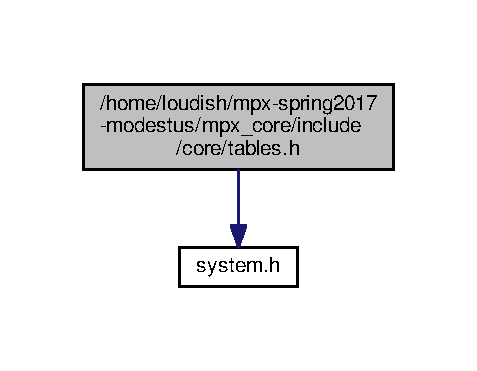
\includegraphics[width=229pt]{tables_8h__incl}
\end{center}
\end{figure}
This graph shows which files directly or indirectly include this file\+:\nopagebreak
\begin{figure}[H]
\begin{center}
\leavevmode
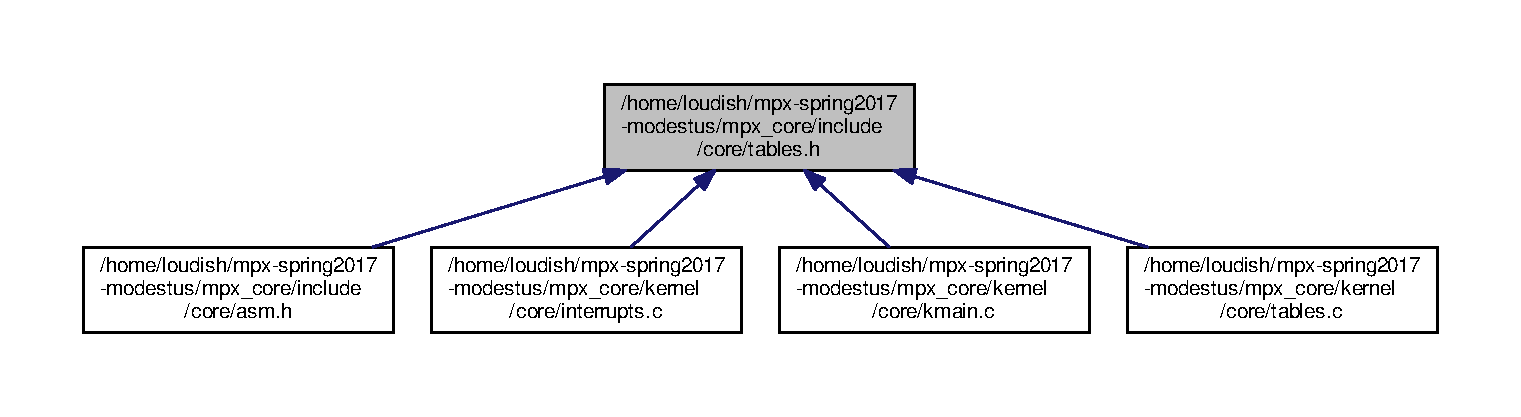
\includegraphics[width=350pt]{tables_8h__dep__incl}
\end{center}
\end{figure}
\subsection*{Data Structures}
\begin{DoxyCompactItemize}
\item 
struct \hyperlink{structidt__entry__struct}{idt\+\_\+entry\+\_\+struct}
\item 
struct \hyperlink{structidt__struct}{idt\+\_\+struct}
\item 
struct \hyperlink{structgdt__descriptor__struct}{gdt\+\_\+descriptor\+\_\+struct}
\item 
struct \hyperlink{structgdt__entry__struct}{gdt\+\_\+entry\+\_\+struct}
\end{DoxyCompactItemize}
\subsection*{Functions}
\begin{DoxyCompactItemize}
\item 
struct \hyperlink{structidt__entry__struct}{idt\+\_\+entry\+\_\+struct} \hyperlink{tables_8h_ad1929ba5e546bde910d88a7c08dc507b}{\+\_\+\+\_\+attribute\+\_\+\+\_\+} ((packed)) idt\+\_\+entry
\item 
void \hyperlink{tables_8h_a9eca3fe1465f8d7d383551d804853139}{idt\+\_\+set\+\_\+gate} (\hyperlink{system_8h_a1026e682ffdadc1701c42cd44ce9efcf}{u8int} idx, \hyperlink{system_8h_a757de76cafbcddaac0d1632902fe4cb8}{u32int} \hyperlink{tables_8h_ab5763c2b18c825c8b8fba44b2e60ddc1}{base}, \hyperlink{system_8h_a863d9497073aad2b991aeab2211d87af}{u16int} sel, \hyperlink{system_8h_a1026e682ffdadc1701c42cd44ce9efcf}{u8int} \hyperlink{tables_8h_a138dda98fcd4738346af61bcca8cf4b4}{flags})
\item 
void \hyperlink{tables_8h_a0b5aee548c88c40ecb07741be1be2e27}{gdt\+\_\+init\+\_\+entry} (int idx, \hyperlink{system_8h_a757de76cafbcddaac0d1632902fe4cb8}{u32int} \hyperlink{tables_8h_ab5763c2b18c825c8b8fba44b2e60ddc1}{base}, \hyperlink{system_8h_a757de76cafbcddaac0d1632902fe4cb8}{u32int} \hyperlink{tables_8h_a68fd3b4f6c14a331ca9b226cbf122e13}{limit}, \hyperlink{system_8h_a1026e682ffdadc1701c42cd44ce9efcf}{u8int} \hyperlink{tables_8h_a360a726ac0b61d9e4e1be3ad34f80244}{access}, \hyperlink{system_8h_a1026e682ffdadc1701c42cd44ce9efcf}{u8int} \hyperlink{tables_8h_a138dda98fcd4738346af61bcca8cf4b4}{flags})
\item 
void \hyperlink{tables_8h_a35fe413107af682030ab7a4b6dff19b8}{init\+\_\+idt} ()
\item 
void \hyperlink{tables_8h_a86bb50044169930202cc403376ef40c3}{init\+\_\+gdt} ()
\end{DoxyCompactItemize}
\subsection*{Variables}
\begin{DoxyCompactItemize}
\item 
\hyperlink{system_8h_a863d9497073aad2b991aeab2211d87af}{u16int} \hyperlink{tables_8h_a0a776dced2c26f16298425cde39f8364}{base\+\_\+low}
\item 
\hyperlink{system_8h_a863d9497073aad2b991aeab2211d87af}{u16int} \hyperlink{tables_8h_ab3f34507900160b4a9b309b4ed039e07}{sselect}
\item 
\hyperlink{system_8h_a1026e682ffdadc1701c42cd44ce9efcf}{u8int} \hyperlink{tables_8h_a94515e42687e7508877c09da81f86860}{zero}
\item 
\hyperlink{system_8h_a1026e682ffdadc1701c42cd44ce9efcf}{u8int} \hyperlink{tables_8h_a138dda98fcd4738346af61bcca8cf4b4}{flags}
\item 
\hyperlink{system_8h_a863d9497073aad2b991aeab2211d87af}{u16int} \hyperlink{tables_8h_a706c81b840522a69ab6e6e941630d5e4}{base\+\_\+high}
\item 
\hyperlink{system_8h_a863d9497073aad2b991aeab2211d87af}{u16int} \hyperlink{tables_8h_a68fd3b4f6c14a331ca9b226cbf122e13}{limit}
\item 
\hyperlink{system_8h_a757de76cafbcddaac0d1632902fe4cb8}{u32int} \hyperlink{tables_8h_ab5763c2b18c825c8b8fba44b2e60ddc1}{base}
\item 
\hyperlink{system_8h_a863d9497073aad2b991aeab2211d87af}{u16int} \hyperlink{tables_8h_af9013229edfb91d4820f66b8df890ce3}{limit\+\_\+low}
\item 
\hyperlink{system_8h_a1026e682ffdadc1701c42cd44ce9efcf}{u8int} \hyperlink{tables_8h_a35c709a004babd09046db9f667ba0646}{base\+\_\+mid}
\item 
\hyperlink{system_8h_a1026e682ffdadc1701c42cd44ce9efcf}{u8int} \hyperlink{tables_8h_a360a726ac0b61d9e4e1be3ad34f80244}{access}
\end{DoxyCompactItemize}


\subsection{Function Documentation}
\index{tables.\+h@{tables.\+h}!\+\_\+\+\_\+attribute\+\_\+\+\_\+@{\+\_\+\+\_\+attribute\+\_\+\+\_\+}}
\index{\+\_\+\+\_\+attribute\+\_\+\+\_\+@{\+\_\+\+\_\+attribute\+\_\+\+\_\+}!tables.\+h@{tables.\+h}}
\subsubsection[{\texorpdfstring{\+\_\+\+\_\+attribute\+\_\+\+\_\+((packed)) idt\+\_\+entry}{__attribute__((packed)) idt_entry}}]{\setlength{\rightskip}{0pt plus 5cm}struct {\bf idt\+\_\+entry\+\_\+struct} \+\_\+\+\_\+attribute\+\_\+\+\_\+ (
\begin{DoxyParamCaption}
\item[{(packed)}]{}
\end{DoxyParamCaption}
)}\hypertarget{tables_8h_ad1929ba5e546bde910d88a7c08dc507b}{}\label{tables_8h_ad1929ba5e546bde910d88a7c08dc507b}
\index{tables.\+h@{tables.\+h}!gdt\+\_\+init\+\_\+entry@{gdt\+\_\+init\+\_\+entry}}
\index{gdt\+\_\+init\+\_\+entry@{gdt\+\_\+init\+\_\+entry}!tables.\+h@{tables.\+h}}
\subsubsection[{\texorpdfstring{gdt\+\_\+init\+\_\+entry(int idx, u32int base, u32int limit, u8int access, u8int flags)}{gdt_init_entry(int idx, u32int base, u32int limit, u8int access, u8int flags)}}]{\setlength{\rightskip}{0pt plus 5cm}void gdt\+\_\+init\+\_\+entry (
\begin{DoxyParamCaption}
\item[{int}]{idx, }
\item[{{\bf u32int}}]{base, }
\item[{{\bf u32int}}]{limit, }
\item[{{\bf u8int}}]{access, }
\item[{{\bf u8int}}]{flags}
\end{DoxyParamCaption}
)}\hypertarget{tables_8h_a0b5aee548c88c40ecb07741be1be2e27}{}\label{tables_8h_a0b5aee548c88c40ecb07741be1be2e27}


Definition at line 57 of file tables.\+c.



References access, and gdt\+\_\+entries.



Referenced by init\+\_\+gdt().


\begin{DoxyCode}
59 \{
60   gdt\_entry *new\_entry = &\hyperlink{tables_8c_ac64ff6d00454e0b88d43b55536418288}{gdt\_entries}[idx];
61   new\_entry->base\_low  = (\hyperlink{tables_8h_ab5763c2b18c825c8b8fba44b2e60ddc1}{base} & 0xFFFF);
62   new\_entry->base\_mid  = (\hyperlink{tables_8h_ab5763c2b18c825c8b8fba44b2e60ddc1}{base} >> 16) & 0xFF;
63   new\_entry->base\_high = (\hyperlink{tables_8h_ab5763c2b18c825c8b8fba44b2e60ddc1}{base} >> 24) & 0xFF;
64   new\_entry->limit\_low = (\hyperlink{tables_8h_a68fd3b4f6c14a331ca9b226cbf122e13}{limit} & 0xFFFF);
65   new\_entry->flags  = (\hyperlink{tables_8h_a68fd3b4f6c14a331ca9b226cbf122e13}{limit} >> 16) & 0xFF;
66   new\_entry->flags |= \hyperlink{tables_8h_a138dda98fcd4738346af61bcca8cf4b4}{flags} & 0xF0;
67   new\_entry->access = \hyperlink{tables_8h_a360a726ac0b61d9e4e1be3ad34f80244}{access};
68 \}
\end{DoxyCode}
\index{tables.\+h@{tables.\+h}!idt\+\_\+set\+\_\+gate@{idt\+\_\+set\+\_\+gate}}
\index{idt\+\_\+set\+\_\+gate@{idt\+\_\+set\+\_\+gate}!tables.\+h@{tables.\+h}}
\subsubsection[{\texorpdfstring{idt\+\_\+set\+\_\+gate(u8int idx, u32int base, u16int sel, u8int flags)}{idt_set_gate(u8int idx, u32int base, u16int sel, u8int flags)}}]{\setlength{\rightskip}{0pt plus 5cm}void idt\+\_\+set\+\_\+gate (
\begin{DoxyParamCaption}
\item[{{\bf u8int}}]{idx, }
\item[{{\bf u32int}}]{base, }
\item[{{\bf u16int}}]{sel, }
\item[{{\bf u8int}}]{flags}
\end{DoxyParamCaption}
)}\hypertarget{tables_8h_a9eca3fe1465f8d7d383551d804853139}{}\label{tables_8h_a9eca3fe1465f8d7d383551d804853139}


Definition at line 27 of file tables.\+c.



References flags, and idt\+\_\+entries.



Referenced by init\+\_\+irq().


\begin{DoxyCode}
29 \{
30   idt\_entry *new\_entry = &\hyperlink{tables_8c_a3c386c59636822ce451be20cc1433a55}{idt\_entries}[idx];
31   new\_entry->base\_low  = (\hyperlink{tables_8h_ab5763c2b18c825c8b8fba44b2e60ddc1}{base} &  0xFFFF);
32   new\_entry->base\_high = (\hyperlink{tables_8h_ab5763c2b18c825c8b8fba44b2e60ddc1}{base} >> 16) & 0xFFFF;
33   new\_entry->sselect   = sel;
34   new\_entry->zero = 0;
35   new\_entry->flags = \hyperlink{tables_8h_a138dda98fcd4738346af61bcca8cf4b4}{flags};
36 \}
\end{DoxyCode}
\index{tables.\+h@{tables.\+h}!init\+\_\+gdt@{init\+\_\+gdt}}
\index{init\+\_\+gdt@{init\+\_\+gdt}!tables.\+h@{tables.\+h}}
\subsubsection[{\texorpdfstring{init\+\_\+gdt()}{init_gdt()}}]{\setlength{\rightskip}{0pt plus 5cm}void init\+\_\+gdt (
\begin{DoxyParamCaption}
{}
\end{DoxyParamCaption}
)}\hypertarget{tables_8h_a86bb50044169930202cc403376ef40c3}{}\label{tables_8h_a86bb50044169930202cc403376ef40c3}


Definition at line 75 of file tables.\+c.



References gdt\+\_\+entries, gdt\+\_\+init\+\_\+entry(), gdt\+\_\+ptr, limit, and write\+\_\+gdt\+\_\+ptr().



Referenced by kmain().


\begin{DoxyCode}
76 \{
77   \hyperlink{tables_8c_aedb4641b02b4a269294e53be7c9b280e}{gdt\_ptr}.limit = 5 * \textcolor{keyword}{sizeof}(gdt\_entry) - 1;
78   \hyperlink{tables_8c_aedb4641b02b4a269294e53be7c9b280e}{gdt\_ptr}.base  = (\hyperlink{system_8h_a757de76cafbcddaac0d1632902fe4cb8}{u32int}) \hyperlink{tables_8c_ac64ff6d00454e0b88d43b55536418288}{gdt\_entries};
79 
80   \hyperlink{system_8h_a757de76cafbcddaac0d1632902fe4cb8}{u32int} \hyperlink{tables_8h_a68fd3b4f6c14a331ca9b226cbf122e13}{limit} = 0xFFFFFFFF;
81   \hyperlink{tables_8c_a0b5aee548c88c40ecb07741be1be2e27}{gdt\_init\_entry}(0, 0, 0, 0, 0);           \textcolor{comment}{//required null segment}
82   \hyperlink{tables_8c_a0b5aee548c88c40ecb07741be1be2e27}{gdt\_init\_entry}(1, 0, limit, 0x9A, 0xCF); \textcolor{comment}{//code segment}
83   \hyperlink{tables_8c_a0b5aee548c88c40ecb07741be1be2e27}{gdt\_init\_entry}(2, 0, limit, 0x92, 0xCF); \textcolor{comment}{//data segment}
84   \hyperlink{tables_8c_a0b5aee548c88c40ecb07741be1be2e27}{gdt\_init\_entry}(3, 0, limit, 0xFA, 0xCF); \textcolor{comment}{//user mode code segment}
85   \hyperlink{tables_8c_a0b5aee548c88c40ecb07741be1be2e27}{gdt\_init\_entry}(4, 0, limit, 0xF2, 0xCF); \textcolor{comment}{//user mode data segment}
86 
87   \hyperlink{tables_8c_ab603373c64fb0a6d51482121d0800be4}{write\_gdt\_ptr}((\hyperlink{system_8h_a757de76cafbcddaac0d1632902fe4cb8}{u32int}) &\hyperlink{tables_8c_aedb4641b02b4a269294e53be7c9b280e}{gdt\_ptr}, \textcolor{keyword}{sizeof}(gdt\_ptr));
88 \}
\end{DoxyCode}
\index{tables.\+h@{tables.\+h}!init\+\_\+idt@{init\+\_\+idt}}
\index{init\+\_\+idt@{init\+\_\+idt}!tables.\+h@{tables.\+h}}
\subsubsection[{\texorpdfstring{init\+\_\+idt()}{init_idt()}}]{\setlength{\rightskip}{0pt plus 5cm}void init\+\_\+idt (
\begin{DoxyParamCaption}
{}
\end{DoxyParamCaption}
)}\hypertarget{tables_8h_a35fe413107af682030ab7a4b6dff19b8}{}\label{tables_8h_a35fe413107af682030ab7a4b6dff19b8}


Definition at line 43 of file tables.\+c.



References idt\+\_\+entries, idt\+\_\+ptr, memset(), and write\+\_\+idt\+\_\+ptr().



Referenced by kmain().


\begin{DoxyCode}
44 \{
45   \hyperlink{tables_8c_a76f617adbc46449bbc39e7b46504b7c4}{idt\_ptr}.limit = 256*\textcolor{keyword}{sizeof}(idt\_descriptor) - 1;
46   \hyperlink{tables_8c_a76f617adbc46449bbc39e7b46504b7c4}{idt\_ptr}.base  = (\hyperlink{system_8h_a757de76cafbcddaac0d1632902fe4cb8}{u32int})\hyperlink{tables_8c_a3c386c59636822ce451be20cc1433a55}{idt\_entries};
47   \hyperlink{string_8h_ace6ee45c30e71865e6eb635200379db9}{memset}(\hyperlink{tables_8c_a3c386c59636822ce451be20cc1433a55}{idt\_entries}, 0, 256*\textcolor{keyword}{sizeof}(idt\_descriptor));
48   
49   \hyperlink{tables_8c_a77fec66a455d3275b67be5c3d7868555}{write\_idt\_ptr}((\hyperlink{system_8h_a757de76cafbcddaac0d1632902fe4cb8}{u32int})&\hyperlink{tables_8c_a76f617adbc46449bbc39e7b46504b7c4}{idt\_ptr});
50 \}
\end{DoxyCode}


\subsection{Variable Documentation}
\index{tables.\+h@{tables.\+h}!access@{access}}
\index{access@{access}!tables.\+h@{tables.\+h}}
\subsubsection[{\texorpdfstring{access}{access}}]{\setlength{\rightskip}{0pt plus 5cm}{\bf u8int} access}\hypertarget{tables_8h_a360a726ac0b61d9e4e1be3ad34f80244}{}\label{tables_8h_a360a726ac0b61d9e4e1be3ad34f80244}


Definition at line 55 of file tables.\+h.



Referenced by gdt\+\_\+init\+\_\+entry().

\index{tables.\+h@{tables.\+h}!base@{base}}
\index{base@{base}!tables.\+h@{tables.\+h}}
\subsubsection[{\texorpdfstring{base}{base}}]{\setlength{\rightskip}{0pt plus 5cm}{\bf u32int} base}\hypertarget{tables_8h_ab5763c2b18c825c8b8fba44b2e60ddc1}{}\label{tables_8h_ab5763c2b18c825c8b8fba44b2e60ddc1}


Definition at line 53 of file tables.\+h.



Referenced by alloc().

\index{tables.\+h@{tables.\+h}!base\+\_\+high@{base\+\_\+high}}
\index{base\+\_\+high@{base\+\_\+high}!tables.\+h@{tables.\+h}}
\subsubsection[{\texorpdfstring{base\+\_\+high}{base_high}}]{\setlength{\rightskip}{0pt plus 5cm}{\bf u8int} base\+\_\+high}\hypertarget{tables_8h_a706c81b840522a69ab6e6e941630d5e4}{}\label{tables_8h_a706c81b840522a69ab6e6e941630d5e4}


Definition at line 56 of file tables.\+h.

\index{tables.\+h@{tables.\+h}!base\+\_\+low@{base\+\_\+low}}
\index{base\+\_\+low@{base\+\_\+low}!tables.\+h@{tables.\+h}}
\subsubsection[{\texorpdfstring{base\+\_\+low}{base_low}}]{\setlength{\rightskip}{0pt plus 5cm}{\bf u16int} base\+\_\+low}\hypertarget{tables_8h_a0a776dced2c26f16298425cde39f8364}{}\label{tables_8h_a0a776dced2c26f16298425cde39f8364}


Definition at line 52 of file tables.\+h.

\index{tables.\+h@{tables.\+h}!base\+\_\+mid@{base\+\_\+mid}}
\index{base\+\_\+mid@{base\+\_\+mid}!tables.\+h@{tables.\+h}}
\subsubsection[{\texorpdfstring{base\+\_\+mid}{base_mid}}]{\setlength{\rightskip}{0pt plus 5cm}{\bf u8int} base\+\_\+mid}\hypertarget{tables_8h_a35c709a004babd09046db9f667ba0646}{}\label{tables_8h_a35c709a004babd09046db9f667ba0646}


Definition at line 54 of file tables.\+h.

\index{tables.\+h@{tables.\+h}!flags@{flags}}
\index{flags@{flags}!tables.\+h@{tables.\+h}}
\subsubsection[{\texorpdfstring{flags}{flags}}]{\setlength{\rightskip}{0pt plus 5cm}{\bf u8int} flags}\hypertarget{tables_8h_a138dda98fcd4738346af61bcca8cf4b4}{}\label{tables_8h_a138dda98fcd4738346af61bcca8cf4b4}


Definition at line 55 of file tables.\+h.



Referenced by idt\+\_\+set\+\_\+gate().

\index{tables.\+h@{tables.\+h}!limit@{limit}}
\index{limit@{limit}!tables.\+h@{tables.\+h}}
\subsubsection[{\texorpdfstring{limit}{limit}}]{\setlength{\rightskip}{0pt plus 5cm}{\bf u16int} limit}\hypertarget{tables_8h_a68fd3b4f6c14a331ca9b226cbf122e13}{}\label{tables_8h_a68fd3b4f6c14a331ca9b226cbf122e13}


Definition at line 52 of file tables.\+h.



Referenced by init\+\_\+gdt().

\index{tables.\+h@{tables.\+h}!limit\+\_\+low@{limit\+\_\+low}}
\index{limit\+\_\+low@{limit\+\_\+low}!tables.\+h@{tables.\+h}}
\subsubsection[{\texorpdfstring{limit\+\_\+low}{limit_low}}]{\setlength{\rightskip}{0pt plus 5cm}{\bf u16int} limit\+\_\+low}\hypertarget{tables_8h_af9013229edfb91d4820f66b8df890ce3}{}\label{tables_8h_af9013229edfb91d4820f66b8df890ce3}


Definition at line 52 of file tables.\+h.

\index{tables.\+h@{tables.\+h}!sselect@{sselect}}
\index{sselect@{sselect}!tables.\+h@{tables.\+h}}
\subsubsection[{\texorpdfstring{sselect}{sselect}}]{\setlength{\rightskip}{0pt plus 5cm}{\bf u16int} sselect}\hypertarget{tables_8h_ab3f34507900160b4a9b309b4ed039e07}{}\label{tables_8h_ab3f34507900160b4a9b309b4ed039e07}


Definition at line 53 of file tables.\+h.

\index{tables.\+h@{tables.\+h}!zero@{zero}}
\index{zero@{zero}!tables.\+h@{tables.\+h}}
\subsubsection[{\texorpdfstring{zero}{zero}}]{\setlength{\rightskip}{0pt plus 5cm}{\bf u8int} zero}\hypertarget{tables_8h_a94515e42687e7508877c09da81f86860}{}\label{tables_8h_a94515e42687e7508877c09da81f86860}


Definition at line 54 of file tables.\+h.


\hypertarget{input_8h}{}\section{/home/loudish/mpx-\/spring2017-\/modestus/mpx\+\_\+core/include/input.h File Reference}
\label{input_8h}\index{/home/loudish/mpx-\/spring2017-\/modestus/mpx\+\_\+core/include/input.\+h@{/home/loudish/mpx-\/spring2017-\/modestus/mpx\+\_\+core/include/input.\+h}}
This graph shows which files directly or indirectly include this file\+:\nopagebreak
\begin{figure}[H]
\begin{center}
\leavevmode
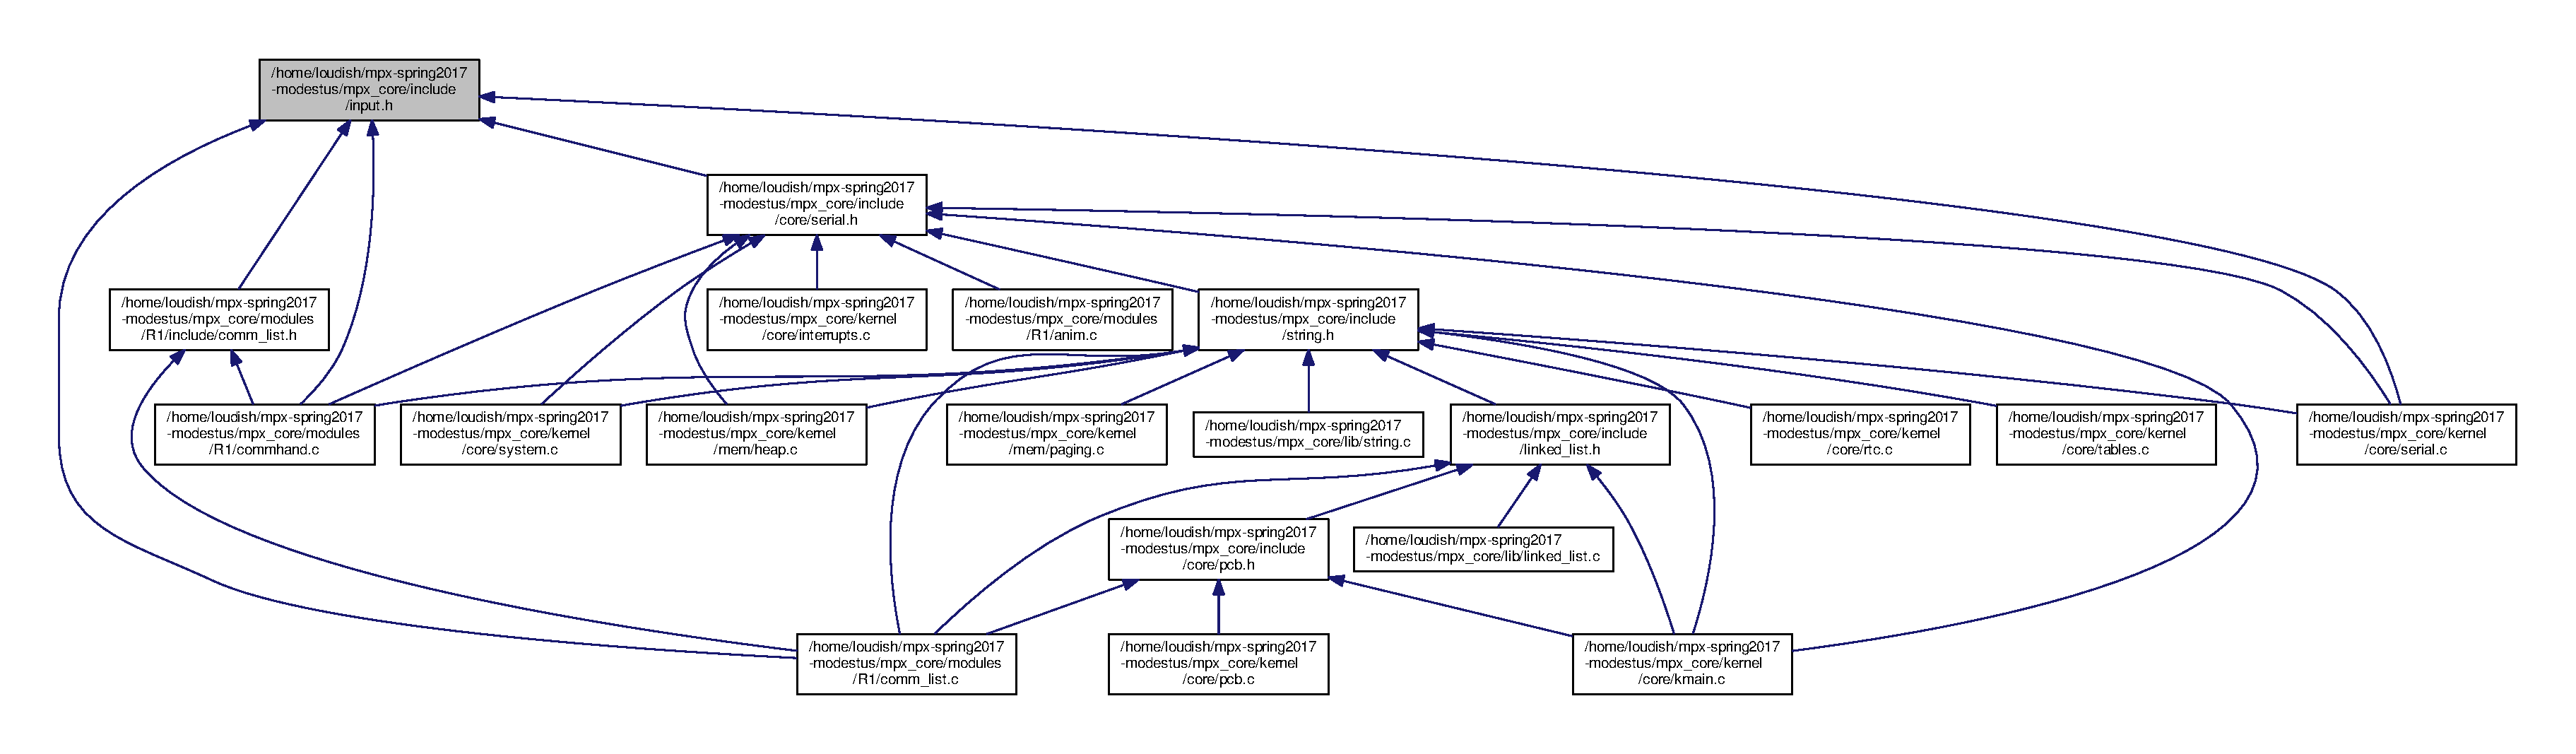
\includegraphics[width=350pt]{input_8h__dep__incl}
\end{center}
\end{figure}
\subsection*{Macros}
\begin{DoxyCompactItemize}
\item 
\#define \hyperlink{input_8h_a1d5dab30b404fab91608086105afc78c}{M\+A\+X\+\_\+\+B\+U\+F\+F\+ER}~128
\item 
\#define \hyperlink{input_8h_a7a9a231e30b47bc0345749c8bd1e5077}{M\+A\+X\+\_\+\+L\+E\+N\+G\+TH}~128
\item 
\#define \hyperlink{input_8h_accdbea14ea06c15e271784368bd993e8}{P\+R\+O\+M\+PT}~\char`\"{}$>$ \char`\"{}
\item 
\#define \hyperlink{input_8h_a629568514359445d2fbda71d70eeb1ce}{B\+A\+C\+K\+S\+P\+A\+CE}~\textquotesingle{}\textbackslash{}177\textquotesingle{}
\item 
\#define \hyperlink{input_8h_abbbe5949f3c1f72e439924f8cf503509}{D\+E\+L\+E\+TE}~\textquotesingle{}\textbackslash{}176\textquotesingle{}
\item 
\#define \hyperlink{input_8h_a4af1b6159e447ba72652bb7fcdfa726e}{E\+SC}~\textquotesingle{}\textbackslash{}033\textquotesingle{}
\item 
\#define \hyperlink{input_8h_a1965eaca47dbf3f87acdafc2208f04eb}{UP}~\textquotesingle{}A\textquotesingle{}
\item 
\#define \hyperlink{input_8h_a4193cd1c8c2e6ebd0e056fa2364a663f}{D\+O\+WN}~\textquotesingle{}B\textquotesingle{}
\item 
\#define \hyperlink{input_8h_a437ef08681e7210d6678427030446a54}{L\+E\+FT}~\textquotesingle{}C\textquotesingle{}
\item 
\#define \hyperlink{input_8h_a80fb826a684cf3f0d306b22aa100ddac}{R\+I\+G\+HT}~\textquotesingle{}D\textquotesingle{}
\item 
\#define \hyperlink{input_8h_a6a0e6b80dd3d5ca395cf58151749f5e2}{R\+E\+T\+U\+RN}~\textquotesingle{}\textbackslash{}r\textquotesingle{}
\item 
\#define \hyperlink{input_8h_a7b99dc1e1c86b4897498c2d436ead1b5}{N\+E\+W\+\_\+\+L\+I\+NE}~\textquotesingle{}\textbackslash{}n\textquotesingle{}
\end{DoxyCompactItemize}


\subsection{Macro Definition Documentation}
\index{input.\+h@{input.\+h}!B\+A\+C\+K\+S\+P\+A\+CE@{B\+A\+C\+K\+S\+P\+A\+CE}}
\index{B\+A\+C\+K\+S\+P\+A\+CE@{B\+A\+C\+K\+S\+P\+A\+CE}!input.\+h@{input.\+h}}
\subsubsection[{\texorpdfstring{B\+A\+C\+K\+S\+P\+A\+CE}{BACKSPACE}}]{\setlength{\rightskip}{0pt plus 5cm}\#define B\+A\+C\+K\+S\+P\+A\+CE~\textquotesingle{}\textbackslash{}177\textquotesingle{}}\hypertarget{input_8h_a629568514359445d2fbda71d70eeb1ce}{}\label{input_8h_a629568514359445d2fbda71d70eeb1ce}


Definition at line 8 of file input.\+h.



Referenced by serial\+\_\+poll().

\index{input.\+h@{input.\+h}!D\+E\+L\+E\+TE@{D\+E\+L\+E\+TE}}
\index{D\+E\+L\+E\+TE@{D\+E\+L\+E\+TE}!input.\+h@{input.\+h}}
\subsubsection[{\texorpdfstring{D\+E\+L\+E\+TE}{DELETE}}]{\setlength{\rightskip}{0pt plus 5cm}\#define D\+E\+L\+E\+TE~\textquotesingle{}\textbackslash{}176\textquotesingle{}}\hypertarget{input_8h_abbbe5949f3c1f72e439924f8cf503509}{}\label{input_8h_abbbe5949f3c1f72e439924f8cf503509}


Definition at line 9 of file input.\+h.



Referenced by serial\+\_\+poll().

\index{input.\+h@{input.\+h}!D\+O\+WN@{D\+O\+WN}}
\index{D\+O\+WN@{D\+O\+WN}!input.\+h@{input.\+h}}
\subsubsection[{\texorpdfstring{D\+O\+WN}{DOWN}}]{\setlength{\rightskip}{0pt plus 5cm}\#define D\+O\+WN~\textquotesingle{}B\textquotesingle{}}\hypertarget{input_8h_a4193cd1c8c2e6ebd0e056fa2364a663f}{}\label{input_8h_a4193cd1c8c2e6ebd0e056fa2364a663f}


Definition at line 12 of file input.\+h.

\index{input.\+h@{input.\+h}!E\+SC@{E\+SC}}
\index{E\+SC@{E\+SC}!input.\+h@{input.\+h}}
\subsubsection[{\texorpdfstring{E\+SC}{ESC}}]{\setlength{\rightskip}{0pt plus 5cm}\#define E\+SC~\textquotesingle{}\textbackslash{}033\textquotesingle{}}\hypertarget{input_8h_a4af1b6159e447ba72652bb7fcdfa726e}{}\label{input_8h_a4af1b6159e447ba72652bb7fcdfa726e}


Definition at line 10 of file input.\+h.



Referenced by serial\+\_\+poll().

\index{input.\+h@{input.\+h}!L\+E\+FT@{L\+E\+FT}}
\index{L\+E\+FT@{L\+E\+FT}!input.\+h@{input.\+h}}
\subsubsection[{\texorpdfstring{L\+E\+FT}{LEFT}}]{\setlength{\rightskip}{0pt plus 5cm}\#define L\+E\+FT~\textquotesingle{}C\textquotesingle{}}\hypertarget{input_8h_a437ef08681e7210d6678427030446a54}{}\label{input_8h_a437ef08681e7210d6678427030446a54}


Definition at line 13 of file input.\+h.

\index{input.\+h@{input.\+h}!M\+A\+X\+\_\+\+B\+U\+F\+F\+ER@{M\+A\+X\+\_\+\+B\+U\+F\+F\+ER}}
\index{M\+A\+X\+\_\+\+B\+U\+F\+F\+ER@{M\+A\+X\+\_\+\+B\+U\+F\+F\+ER}!input.\+h@{input.\+h}}
\subsubsection[{\texorpdfstring{M\+A\+X\+\_\+\+B\+U\+F\+F\+ER}{MAX_BUFFER}}]{\setlength{\rightskip}{0pt plus 5cm}\#define M\+A\+X\+\_\+\+B\+U\+F\+F\+ER~128}\hypertarget{input_8h_a1d5dab30b404fab91608086105afc78c}{}\label{input_8h_a1d5dab30b404fab91608086105afc78c}


Definition at line 5 of file input.\+h.

\index{input.\+h@{input.\+h}!M\+A\+X\+\_\+\+L\+E\+N\+G\+TH@{M\+A\+X\+\_\+\+L\+E\+N\+G\+TH}}
\index{M\+A\+X\+\_\+\+L\+E\+N\+G\+TH@{M\+A\+X\+\_\+\+L\+E\+N\+G\+TH}!input.\+h@{input.\+h}}
\subsubsection[{\texorpdfstring{M\+A\+X\+\_\+\+L\+E\+N\+G\+TH}{MAX_LENGTH}}]{\setlength{\rightskip}{0pt plus 5cm}\#define M\+A\+X\+\_\+\+L\+E\+N\+G\+TH~128}\hypertarget{input_8h_a7a9a231e30b47bc0345749c8bd1e5077}{}\label{input_8h_a7a9a231e30b47bc0345749c8bd1e5077}


Definition at line 6 of file input.\+h.



Referenced by exec\+\_\+comm(), and init\+\_\+commhand().

\index{input.\+h@{input.\+h}!N\+E\+W\+\_\+\+L\+I\+NE@{N\+E\+W\+\_\+\+L\+I\+NE}}
\index{N\+E\+W\+\_\+\+L\+I\+NE@{N\+E\+W\+\_\+\+L\+I\+NE}!input.\+h@{input.\+h}}
\subsubsection[{\texorpdfstring{N\+E\+W\+\_\+\+L\+I\+NE}{NEW_LINE}}]{\setlength{\rightskip}{0pt plus 5cm}\#define N\+E\+W\+\_\+\+L\+I\+NE~\textquotesingle{}\textbackslash{}n\textquotesingle{}}\hypertarget{input_8h_a7b99dc1e1c86b4897498c2d436ead1b5}{}\label{input_8h_a7b99dc1e1c86b4897498c2d436ead1b5}


Definition at line 16 of file input.\+h.



Referenced by serial\+\_\+poll().

\index{input.\+h@{input.\+h}!P\+R\+O\+M\+PT@{P\+R\+O\+M\+PT}}
\index{P\+R\+O\+M\+PT@{P\+R\+O\+M\+PT}!input.\+h@{input.\+h}}
\subsubsection[{\texorpdfstring{P\+R\+O\+M\+PT}{PROMPT}}]{\setlength{\rightskip}{0pt plus 5cm}\#define P\+R\+O\+M\+PT~\char`\"{}$>$ \char`\"{}}\hypertarget{input_8h_accdbea14ea06c15e271784368bd993e8}{}\label{input_8h_accdbea14ea06c15e271784368bd993e8}


Definition at line 7 of file input.\+h.



Referenced by init\+\_\+commhand().

\index{input.\+h@{input.\+h}!R\+E\+T\+U\+RN@{R\+E\+T\+U\+RN}}
\index{R\+E\+T\+U\+RN@{R\+E\+T\+U\+RN}!input.\+h@{input.\+h}}
\subsubsection[{\texorpdfstring{R\+E\+T\+U\+RN}{RETURN}}]{\setlength{\rightskip}{0pt plus 5cm}\#define R\+E\+T\+U\+RN~\textquotesingle{}\textbackslash{}r\textquotesingle{}}\hypertarget{input_8h_a6a0e6b80dd3d5ca395cf58151749f5e2}{}\label{input_8h_a6a0e6b80dd3d5ca395cf58151749f5e2}


Definition at line 15 of file input.\+h.



Referenced by serial\+\_\+poll().

\index{input.\+h@{input.\+h}!R\+I\+G\+HT@{R\+I\+G\+HT}}
\index{R\+I\+G\+HT@{R\+I\+G\+HT}!input.\+h@{input.\+h}}
\subsubsection[{\texorpdfstring{R\+I\+G\+HT}{RIGHT}}]{\setlength{\rightskip}{0pt plus 5cm}\#define R\+I\+G\+HT~\textquotesingle{}D\textquotesingle{}}\hypertarget{input_8h_a80fb826a684cf3f0d306b22aa100ddac}{}\label{input_8h_a80fb826a684cf3f0d306b22aa100ddac}


Definition at line 14 of file input.\+h.

\index{input.\+h@{input.\+h}!UP@{UP}}
\index{UP@{UP}!input.\+h@{input.\+h}}
\subsubsection[{\texorpdfstring{UP}{UP}}]{\setlength{\rightskip}{0pt plus 5cm}\#define UP~\textquotesingle{}A\textquotesingle{}}\hypertarget{input_8h_a1965eaca47dbf3f87acdafc2208f04eb}{}\label{input_8h_a1965eaca47dbf3f87acdafc2208f04eb}


Definition at line 11 of file input.\+h.


\hypertarget{linked__list_8h}{}\section{/home/loudish/mpx-\/spring2017-\/modestus/mpx\+\_\+core/include/linked\+\_\+list.h File Reference}
\label{linked__list_8h}\index{/home/loudish/mpx-\/spring2017-\/modestus/mpx\+\_\+core/include/linked\+\_\+list.\+h@{/home/loudish/mpx-\/spring2017-\/modestus/mpx\+\_\+core/include/linked\+\_\+list.\+h}}
{\ttfamily \#include \char`\"{}string.\+h\char`\"{}}\\*
{\ttfamily \#include $<$core/mpx\+\_\+supt.\+h$>$}\\*
Include dependency graph for linked\+\_\+list.\+h\+:\nopagebreak
\begin{figure}[H]
\begin{center}
\leavevmode
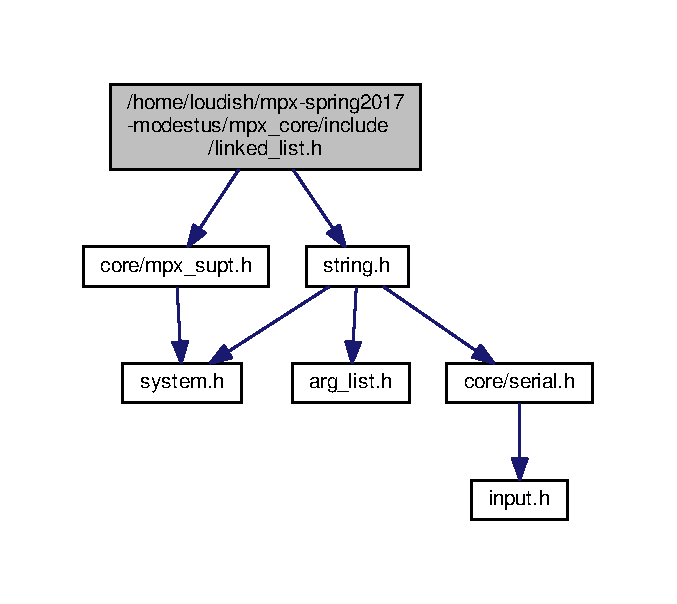
\includegraphics[width=325pt]{linked__list_8h__incl}
\end{center}
\end{figure}
This graph shows which files directly or indirectly include this file\+:\nopagebreak
\begin{figure}[H]
\begin{center}
\leavevmode
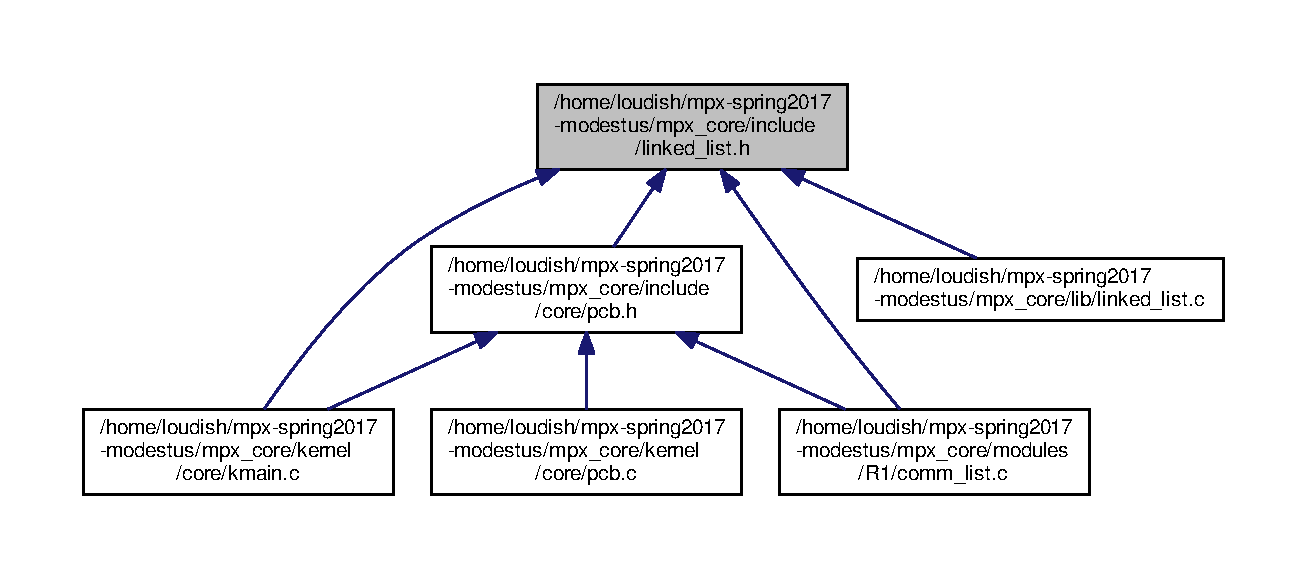
\includegraphics[width=350pt]{linked__list_8h__dep__incl}
\end{center}
\end{figure}
\subsection*{Data Structures}
\begin{DoxyCompactItemize}
\item 
struct \hyperlink{structs__ll__node}{node\+\_\+t}
\begin{DoxyCompactList}\small\item\em struct for a node of the linked list \end{DoxyCompactList}\item 
struct \hyperlink{structs__ll}{linked\+List\+\_\+t}
\begin{DoxyCompactList}\small\item\em struct definition for the linked list \end{DoxyCompactList}\end{DoxyCompactItemize}
\subsection*{Macros}
\begin{DoxyCompactItemize}
\item 
\#define \hyperlink{linked__list_8h_a4bdabb4388c831c1f8c4d31e67801e74}{M\+A\+X\+\_\+\+N\+U\+M\+\_\+\+O\+F\+\_\+\+L\+L\+\_\+\+N\+O\+D\+ES}~256
\item 
\#define \hyperlink{linked__list_8h_a33fa4884df656ed557638b8bd9585a7e}{V\+A\+R\+I\+A\+B\+L\+E\+\_\+\+L\+L\+\_\+\+L\+E\+N\+G\+TH}(L\+I\+S\+T\+\_\+\+L\+E\+N\+G\+TH)
\end{DoxyCompactItemize}
\subsection*{Functions}
\begin{DoxyCompactItemize}
\item 
void \hyperlink{linked__list_8h_a88e42961d952fbe5abb7e8cb26c916cc}{init\+Linked\+List} (\hyperlink{structlinked_list__t}{linked\+List\+\_\+t} $\ast$list)
\begin{DoxyCompactList}\small\item\em initilize list and the optional array that backs the list \end{DoxyCompactList}\item 
\hyperlink{structnode__t}{node\+\_\+t} $\ast$ \hyperlink{linked__list_8h_a20871a48a5ca68065f74200de139228b}{insert\+After\+Node} (\hyperlink{structnode__t}{node\+\_\+t} $\ast$preceeding\+Node, \hyperlink{structnode__t}{node\+\_\+t} $\ast$new\+Node)
\begin{DoxyCompactList}\small\item\em insert a node into the parent list of the preceeding\+Node after preceeding\+Node \end{DoxyCompactList}\item 
\hyperlink{structnode__t}{node\+\_\+t} $\ast$ \hyperlink{linked__list_8h_a04df23f8eb8508551930249bad9f159a}{insert\+Before\+Node} (\hyperlink{structnode__t}{node\+\_\+t} $\ast$node\+To\+Follow, \hyperlink{structnode__t}{node\+\_\+t} $\ast$new\+Node)
\begin{DoxyCompactList}\small\item\em insert a node into the parent list of the node\+To\+Follow before node\+To\+Follow \end{DoxyCompactList}\item 
\hyperlink{structnode__t}{node\+\_\+t} $\ast$ \hyperlink{linked__list_8h_a40b9cae4db9ce33443e541191e75f540}{insert\+Node} (\hyperlink{structlinked_list__t}{linked\+List\+\_\+t} $\ast$list, \hyperlink{structnode__t}{node\+\_\+t} $\ast$new\+Node)
\begin{DoxyCompactList}\small\item\em Will insert the node into the list. This function will attempt to call the list\textquotesingle{}s \hyperlink{linked__list_8c_a45d030386936adffa3eb5586ce93d131}{insert comparison} function if defined. The function will insert the new node into the list after this function returns $>$ 0. If the \hyperlink{linked__list_8c_a45d030386936adffa3eb5586ce93d131}{insert comparison} function is not defined for this list, the inserting function will placed the new node at the end of the list before the tail. \end{DoxyCompactList}\item 
\hyperlink{structnode__t}{node\+\_\+t} $\ast$ \hyperlink{linked__list_8h_a042e8aa38eb81453dd7e81ade7d38b5b}{make\+New\+Node} (\hyperlink{structlinked_list__t}{linked\+List\+\_\+t} $\ast$list, void $\ast$data)
\begin{DoxyCompactList}\small\item\em get new node, allocate a new node or find an unused node from the list\textquotesingle{}s pool \end{DoxyCompactList}\item 
\hyperlink{structnode__t}{node\+\_\+t} $\ast$ \hyperlink{linked__list_8h_a1573ed6fa569b80577b596e78cd90b4a}{move\+Node\+To\+New\+List} (\hyperlink{structnode__t}{node\+\_\+t} $\ast$node\+To\+Move, \hyperlink{structlinked_list__t}{linked\+List\+\_\+t} $\ast$new\+List)
\begin{DoxyCompactList}\small\item\em If a node needs to move lists and lists are array backed, instead of just moving preceeding and suceeding pointers of the node, the node actaully needs to move backing arrays so one list\textquotesingle{}s nodes are not the only ones being consumed. The equivalent process will be to execute the parent list\textquotesingle{}s remove\+Node funcion, execute the make\+New\+Node function on the new\+List, copy all structure members to the new node, and return the new node. The list of node\+To\+Move free\+Node\+Func will be called with node\+To\+Mov as the argument. If the lists are not array backed, the function simply removes the node from its containing list and calls insert\+Node on the new list. \end{DoxyCompactList}\item 
void \hyperlink{linked__list_8h_a3b6f817f74d12d2cf4a35405f447c73d}{set\+Free\+Function} (\hyperlink{structlinked_list__t}{linked\+List\+\_\+t} $\ast$list, int($\ast$new\+Free\+Func)(\hyperlink{structnode__t}{node\+\_\+t} $\ast$))
\begin{DoxyCompactList}\small\item\em sets the function whose job it is to free the node\textquotesingle{}s memory \end{DoxyCompactList}\item 
void \hyperlink{linked__list_8h_a45d030386936adffa3eb5586ce93d131}{set\+Insert\+Comparison\+Function} (\hyperlink{structlinked_list__t}{linked\+List\+\_\+t} $\ast$list, int($\ast$new\+Comp\+Func)(void $\ast$, void $\ast$))
\begin{DoxyCompactList}\small\item\em takes in a function pointer and sets the library shared comparison pointer \end{DoxyCompactList}\item 
void \hyperlink{group___r2_gafc8969d7969f61c928a01f4c302e669b}{set\+Print\+Function} (\hyperlink{structlinked_list__t}{linked\+List\+\_\+t} $\ast$list, void($\ast$new\+Print\+Func)(void $\ast$))
\begin{DoxyCompactList}\small\item\em sets the function whose job it is to print the list to the screen. \end{DoxyCompactList}\item 
void \hyperlink{linked__list_8h_a12e5138ac02af0f6b42ff2f1b29c610a}{set\+Search\+Comparison\+Function} (\hyperlink{structlinked_list__t}{linked\+List\+\_\+t} $\ast$list, int($\ast$new\+Search\+Func)(void $\ast$, void $\ast$))
\begin{DoxyCompactList}\small\item\em sets the function whose job it is to compare the input data with the data in the list. the first void parameter will always be the data contained in the list, the second will be the data passed to the search function. \end{DoxyCompactList}\item 
\hyperlink{structnode__t}{node\+\_\+t} $\ast$ \hyperlink{linked__list_8h_ad225d0f3d9e1b59a58117ba0bc491189}{remove\+Node} (\hyperlink{structnode__t}{node\+\_\+t} $\ast$node\+To\+Remove)
\begin{DoxyCompactList}\small\item\em will remove the node from the list. the list hierarchy will change to reflect the missing node. \end{DoxyCompactList}\item 
\hyperlink{structnode__t}{node\+\_\+t} $\ast$ \hyperlink{linked__list_8h_a75ff37d4b2282fa64cb59415e17f8ee5}{search\+List} (\hyperlink{structlinked_list__t}{linked\+List\+\_\+t} $\ast$list\+To\+Search, void $\ast$data)
\begin{DoxyCompactList}\small\item\em goes through the list using the list\textquotesingle{}s comparison function to find the node which matches the data. if the search function is undefined for this list, the function returns null immedietly. \end{DoxyCompactList}\item 
void \hyperlink{linked__list_8h_a9bbec3837a303ae4bbc5eafb23ead2d5}{print\+List} (\hyperlink{structlinked_list__t}{linked\+List\+\_\+t} $\ast$list)
\begin{DoxyCompactList}\small\item\em test function to show list functionality. uses const char$\ast$ as test data \end{DoxyCompactList}\item 
void \hyperlink{linked__list_8h_a0a60ac1fe6e5055de61277ac9703b13e}{list\+Test} ()
\begin{DoxyCompactList}\small\item\em test the linked\+\_\+list class with const char$\ast$ data and output to screen the results of the test \end{DoxyCompactList}\end{DoxyCompactItemize}
\subsection*{Variables}
\begin{DoxyCompactItemize}
\item 
struct \hyperlink{structs__ll__node}{s\+\_\+ll\+\_\+node} \hyperlink{linked__list_8h_aaa4b117a86b9205e66f2cde318c1f01e}{\+\_\+\+\_\+attribute\+\_\+\+\_\+}
\end{DoxyCompactItemize}


\subsection{Detailed Description}
This module provides a generic linked list that can be array backed or use dynamic allocation 

\subsection{Macro Definition Documentation}
\index{linked\+\_\+list.\+h@{linked\+\_\+list.\+h}!M\+A\+X\+\_\+\+N\+U\+M\+\_\+\+O\+F\+\_\+\+L\+L\+\_\+\+N\+O\+D\+ES@{M\+A\+X\+\_\+\+N\+U\+M\+\_\+\+O\+F\+\_\+\+L\+L\+\_\+\+N\+O\+D\+ES}}
\index{M\+A\+X\+\_\+\+N\+U\+M\+\_\+\+O\+F\+\_\+\+L\+L\+\_\+\+N\+O\+D\+ES@{M\+A\+X\+\_\+\+N\+U\+M\+\_\+\+O\+F\+\_\+\+L\+L\+\_\+\+N\+O\+D\+ES}!linked\+\_\+list.\+h@{linked\+\_\+list.\+h}}
\subsubsection[{\texorpdfstring{M\+A\+X\+\_\+\+N\+U\+M\+\_\+\+O\+F\+\_\+\+L\+L\+\_\+\+N\+O\+D\+ES}{MAX_NUM_OF_LL_NODES}}]{\setlength{\rightskip}{0pt plus 5cm}\#define M\+A\+X\+\_\+\+N\+U\+M\+\_\+\+O\+F\+\_\+\+L\+L\+\_\+\+N\+O\+D\+ES~256}\hypertarget{linked__list_8h_a4bdabb4388c831c1f8c4d31e67801e74}{}\label{linked__list_8h_a4bdabb4388c831c1f8c4d31e67801e74}


Definition at line 22 of file linked\+\_\+list.\+h.



Referenced by init\+Linked\+List(), and make\+New\+Node().

\index{linked\+\_\+list.\+h@{linked\+\_\+list.\+h}!V\+A\+R\+I\+A\+B\+L\+E\+\_\+\+L\+L\+\_\+\+L\+E\+N\+G\+TH@{V\+A\+R\+I\+A\+B\+L\+E\+\_\+\+L\+L\+\_\+\+L\+E\+N\+G\+TH}}
\index{V\+A\+R\+I\+A\+B\+L\+E\+\_\+\+L\+L\+\_\+\+L\+E\+N\+G\+TH@{V\+A\+R\+I\+A\+B\+L\+E\+\_\+\+L\+L\+\_\+\+L\+E\+N\+G\+TH}!linked\+\_\+list.\+h@{linked\+\_\+list.\+h}}
\subsubsection[{\texorpdfstring{V\+A\+R\+I\+A\+B\+L\+E\+\_\+\+L\+L\+\_\+\+L\+E\+N\+G\+TH}{VARIABLE_LL_LENGTH}}]{\setlength{\rightskip}{0pt plus 5cm}\#define V\+A\+R\+I\+A\+B\+L\+E\+\_\+\+L\+L\+\_\+\+L\+E\+N\+G\+TH(
\begin{DoxyParamCaption}
\item[{}]{L\+I\+S\+T\+\_\+\+L\+E\+N\+G\+TH}
\end{DoxyParamCaption}
)}\hypertarget{linked__list_8h_a33fa4884df656ed557638b8bd9585a7e}{}\label{linked__list_8h_a33fa4884df656ed557638b8bd9585a7e}
{\bfseries Value\+:}
\begin{DoxyCode}
\{ \(\backslash\)
    typedef \textcolor{keyword}{struct }s\_ll\_##LIST\_LENGTH##\_t linkedList\_##LIST\_LENGTH##\_t \(\backslash\)
    struct s\_ll\_##LIST\_LENGTH##\_t \(\backslash\)
    \{ \(\backslash\)
        node\_t head; \(\backslash\)
        node\_t tail; \(\backslash\)
        int (*searchCompFunc)(\textcolor{keywordtype}{void}*, \textcolor{keywordtype}{void}*); \(\backslash\)
        int (*comparisonFunc)(\textcolor{keywordtype}{void}*, \textcolor{keywordtype}{void}*); \(\backslash\)
        int (*freeNodeFunc)(\hyperlink{structnode__t}{node\_t} *nodeToFree); \(\backslash\)
        void (*\hyperlink{linked__list_8h_a9bbec3837a303ae4bbc5eafb23ead2d5}{printList})(\textcolor{keywordtype}{void}*); \hyperlink{system_8h_a7c94ea6f8948649f8d181ae55911eeaf}{\(\backslash\)}
\hyperlink{system_8h_a7c94ea6f8948649f8d181ae55911eeaf}{        size\_t} length; \(\backslash\)
        unsigned \textcolor{keywordtype}{int} numNodesInUse; \(\backslash\)
        node\_t backingArray[LIST\_LENGTH]; \(\backslash\)
    \}; \(\backslash\)
\}
\end{DoxyCode}
defines a macro that will generate a new type that has a different array backing size, new type has the name linked\+List\+\_\+$<$list\+\_\+length$>$\+\_\+t 

Definition at line 81 of file linked\+\_\+list.\+h.



\subsection{Function Documentation}
\index{linked\+\_\+list.\+h@{linked\+\_\+list.\+h}!init\+Linked\+List@{init\+Linked\+List}}
\index{init\+Linked\+List@{init\+Linked\+List}!linked\+\_\+list.\+h@{linked\+\_\+list.\+h}}
\subsubsection[{\texorpdfstring{init\+Linked\+List(linked\+List\+\_\+t $\ast$list)}{initLinkedList(linkedList_t *list)}}]{\setlength{\rightskip}{0pt plus 5cm}void init\+Linked\+List (
\begin{DoxyParamCaption}
\item[{{\bf linked\+List\+\_\+t} $\ast$}]{list}
\end{DoxyParamCaption}
)}\hypertarget{linked__list_8h_a88e42961d952fbe5abb7e8cb26c916cc}{}\label{linked__list_8h_a88e42961d952fbe5abb7e8cb26c916cc}


initilize list and the optional array that backs the list 


\begin{DoxyParams}{Parameters}
{\em list} & pointer to list \\
\hline
\end{DoxyParams}


Definition at line 3 of file linked\+\_\+list.\+c.



References M\+A\+X\+\_\+\+N\+U\+M\+\_\+\+O\+F\+\_\+\+L\+L\+\_\+\+N\+O\+D\+ES.



Referenced by init\+P\+C\+B\+Queues(), and list\+Test().


\begin{DoxyCode}
4 \{
5 \textcolor{preprocessor}{#ifdef LL\_IS\_ARRAY\_BACKED}
6     \textcolor{keywordtype}{int} i;
7     \textcolor{keywordflow}{for}(i=0; i < \hyperlink{linked__list_8h_a4bdabb4388c831c1f8c4d31e67801e74}{MAX\_NUM\_OF\_LL\_NODES}; i++)
8     \{
9         list->backingArray[i].data=0;
10         list->backingArray[i].inUse=0;
11         list->backingArray[i].next=0;
12         list->backingArray[i].prev=0;
13         list->backingArray[i].parentList = list;
14     \}
15 
16     list->head.parentList = list;
17     list->head.inUse=1;
18 
19     list->tail.parentList = list;
20     list->tail.inUse=1;
21 \textcolor{preprocessor}{#endif}
22 
23     list->head.data=0;
24     list->head.next =
25         list->head.prev = &list->tail;
26 
27     list->tail.data=0;
28     list->tail.next =
29         list->tail.prev = &list->head;
30 
31     list->length = 0;
32     list->insertCompFunc = 0;
33     list->freeNodeFunc = 0;
34     list->searchCompFunc = 0;
35 \}
\end{DoxyCode}
\index{linked\+\_\+list.\+h@{linked\+\_\+list.\+h}!insert\+After\+Node@{insert\+After\+Node}}
\index{insert\+After\+Node@{insert\+After\+Node}!linked\+\_\+list.\+h@{linked\+\_\+list.\+h}}
\subsubsection[{\texorpdfstring{insert\+After\+Node(node\+\_\+t $\ast$preceeding\+Node, node\+\_\+t $\ast$new\+Node)}{insertAfterNode(node_t *preceedingNode, node_t *newNode)}}]{\setlength{\rightskip}{0pt plus 5cm}{\bf node\+\_\+t}$\ast$ insert\+After\+Node (
\begin{DoxyParamCaption}
\item[{{\bf node\+\_\+t} $\ast$}]{preceeding\+Node, }
\item[{{\bf node\+\_\+t} $\ast$}]{new\+Node}
\end{DoxyParamCaption}
)}\hypertarget{linked__list_8h_a20871a48a5ca68065f74200de139228b}{}\label{linked__list_8h_a20871a48a5ca68065f74200de139228b}


insert a node into the parent list of the preceeding\+Node after preceeding\+Node 


\begin{DoxyParams}{Parameters}
{\em preceeding\+Node} & node to insert the new node afterwards \\
\hline
{\em new\+Node} & the new node to insert. if the list is array backed, the new\+Node will be copied to the list\textquotesingle{}s node pool if it currently does not reside there \\
\hline
\end{DoxyParams}
\begin{DoxyReturn}{Returns}
pointer to node inserted in the parent list of preceeding\+Node, null if insertion failed 
\end{DoxyReturn}


Definition at line 78 of file linked\+\_\+list.\+c.



References move\+Node\+To\+New\+List().


\begin{DoxyCode}
79 \{
80 \textcolor{preprocessor}{#ifdef LL\_IS\_ARRAY\_BACKED}
81     \textcolor{keywordflow}{if}(preceedingNode->parentList != newNode->parentList)
82     \{
83         \textcolor{comment}{//if the node to insert is not apart of the list to insert after, the function moveNodeToNewList
       makes a}
84             \textcolor{comment}{//new node in the parent list of the preceedingNode and recursively calls this function with
       the newly moved node}
85         \textcolor{keywordflow}{return} \hyperlink{linked__list_8c_a20871a48a5ca68065f74200de139228b}{insertAfterNode}(preceedingNode,
86                             \hyperlink{linked__list_8c_a1573ed6fa569b80577b596e78cd90b4a}{moveNodeToNewList}(newNode, preceedingNode->parentList));
87     \}
88 \textcolor{preprocessor}{#endif}
89 
90     newNode->next = preceedingNode->next;
91     newNode->prev = preceedingNode;
92 
93     newNode->next->prev = newNode;
94     newNode->prev->next = newNode;
95 
96     \textcolor{keywordflow}{return} newNode;
97 \}
\end{DoxyCode}
\index{linked\+\_\+list.\+h@{linked\+\_\+list.\+h}!insert\+Before\+Node@{insert\+Before\+Node}}
\index{insert\+Before\+Node@{insert\+Before\+Node}!linked\+\_\+list.\+h@{linked\+\_\+list.\+h}}
\subsubsection[{\texorpdfstring{insert\+Before\+Node(node\+\_\+t $\ast$node\+To\+Follow, node\+\_\+t $\ast$new\+Node)}{insertBeforeNode(node_t *nodeToFollow, node_t *newNode)}}]{\setlength{\rightskip}{0pt plus 5cm}{\bf node\+\_\+t}$\ast$ insert\+Before\+Node (
\begin{DoxyParamCaption}
\item[{{\bf node\+\_\+t} $\ast$}]{node\+To\+Follow, }
\item[{{\bf node\+\_\+t} $\ast$}]{new\+Node}
\end{DoxyParamCaption}
)}\hypertarget{linked__list_8h_a04df23f8eb8508551930249bad9f159a}{}\label{linked__list_8h_a04df23f8eb8508551930249bad9f159a}


insert a node into the parent list of the node\+To\+Follow before node\+To\+Follow 


\begin{DoxyParams}{Parameters}
{\em node\+To\+Follow} & node to insert the new\+Node before \\
\hline
{\em new\+Node} & the new node to insert. if the list is array backed, the new\+Node will be copied to the list\textquotesingle{}s node pool if it currently does not reside there \\
\hline
\end{DoxyParams}
\begin{DoxyReturn}{Returns}
pointer to node inserted in the parent list of node\+To\+Follow, null if insertion failed 
\end{DoxyReturn}


Definition at line 99 of file linked\+\_\+list.\+c.



References move\+Node\+To\+New\+List().



Referenced by insert\+Node().


\begin{DoxyCode}
100 \{
101 \textcolor{preprocessor}{#ifdef LL\_IS\_ARRAY\_BACKED}
102     \textcolor{keywordflow}{if}(nodeToFollow->parentList != newNode->parentList)
103     \{
104         \textcolor{comment}{//if the node to insert is not apart of the list to insert after, the function moveNodeToNewList
       makes a}
105             \textcolor{comment}{//new node in the parent list of the preceedingNode and recursively calls this function with
       the newly moved node}
106         \textcolor{keywordflow}{return} \hyperlink{linked__list_8c_a04df23f8eb8508551930249bad9f159a}{insertBeforeNode}(nodeToFollow,
107                             \hyperlink{linked__list_8c_a1573ed6fa569b80577b596e78cd90b4a}{moveNodeToNewList}(newNode, nodeToFollow->parentList));
108     \}
109 \textcolor{preprocessor}{#endif}
110 
111     newNode->next = nodeToFollow;
112     newNode->prev = nodeToFollow->prev;
113 
114     newNode->next->prev = newNode;
115     newNode->prev->next = newNode;
116 
117     \textcolor{keywordflow}{return} newNode;
118 \}
\end{DoxyCode}
\index{linked\+\_\+list.\+h@{linked\+\_\+list.\+h}!insert\+Node@{insert\+Node}}
\index{insert\+Node@{insert\+Node}!linked\+\_\+list.\+h@{linked\+\_\+list.\+h}}
\subsubsection[{\texorpdfstring{insert\+Node(linked\+List\+\_\+t $\ast$list, node\+\_\+t $\ast$new\+Node)}{insertNode(linkedList_t *list, node_t *newNode)}}]{\setlength{\rightskip}{0pt plus 5cm}{\bf node\+\_\+t}$\ast$ insert\+Node (
\begin{DoxyParamCaption}
\item[{{\bf linked\+List\+\_\+t} $\ast$}]{list, }
\item[{{\bf node\+\_\+t} $\ast$}]{new\+Node}
\end{DoxyParamCaption}
)}\hypertarget{linked__list_8h_a40b9cae4db9ce33443e541191e75f540}{}\label{linked__list_8h_a40b9cae4db9ce33443e541191e75f540}


Will insert the node into the list. This function will attempt to call the list\textquotesingle{}s \hyperlink{linked__list_8c_a45d030386936adffa3eb5586ce93d131}{insert comparison} function if defined. The function will insert the new node into the list after this function returns $>$ 0. If the \hyperlink{linked__list_8c_a45d030386936adffa3eb5586ce93d131}{insert comparison} function is not defined for this list, the inserting function will placed the new node at the end of the list before the tail. 


\begin{DoxyParams}{Parameters}
{\em list} & list to place the node \\
\hline
{\em new\+Node} & the new node to insert. if the list is array backed, the new\+Node will be copied to the list\textquotesingle{}s node pool if it currently does not reside there \\
\hline
\end{DoxyParams}
\begin{DoxyReturn}{Returns}
pointer to the node in the new list, or null if inserting failed. 
\end{DoxyReturn}


Definition at line 173 of file linked\+\_\+list.\+c.



References insert\+Before\+Node(), and move\+Node\+To\+New\+List().



Referenced by insert\+P\+C\+B(), list\+Test(), move\+Node\+To\+New\+List(), and setup\+P\+C\+B().


\begin{DoxyCode}
174 \{
175     \textcolor{comment}{//if newNode is not valid, do not insert any node}
176     \textcolor{keywordflow}{if}(!newNode)
177     \{
178         \textcolor{keywordflow}{return} 0;
179     \}
180 
181 \textcolor{preprocessor}{#ifdef LL\_IS\_ARRAY\_BACKED}
182     \textcolor{keywordflow}{if}(newNode->parentList != list)
183     \{
184         \textcolor{comment}{//if the node to insert is not apart of the list to insert after, the function moveNodeToNewList
       makes a}
185             \textcolor{comment}{//new node in the parent list of the preceedingNode and recursively calls this function with
       the newly moved node}
186         \textcolor{keywordflow}{return} \hyperlink{linked__list_8c_a40b9cae4db9ce33443e541191e75f540}{insertNode}(list, \hyperlink{linked__list_8c_a1573ed6fa569b80577b596e78cd90b4a}{moveNodeToNewList}(newNode, list));
187     \}
188 \textcolor{preprocessor}{#endif}
189 
190     \textcolor{keywordflow}{if}(list->insertCompFunc)
191     \{
192         \hyperlink{structnode__t}{node\_t} * itNode = list->head.next;
193         \textcolor{keywordflow}{for}(; itNode != &(list->tail); itNode = itNode->next)
194         \{
195             \textcolor{keywordtype}{int} result = ((*(list->insertCompFunc))(itNode->data, newNode->data));
196             \textcolor{keywordflow}{if}(result > 0)
197             \{
198                 list->length++;
199                 \textcolor{keywordflow}{return} \hyperlink{linked__list_8c_a04df23f8eb8508551930249bad9f159a}{insertBeforeNode}(itNode, newNode);
200             \}
201         \}
202     \}
203     \textcolor{keywordflow}{return} \hyperlink{linked__list_8c_a04df23f8eb8508551930249bad9f159a}{insertBeforeNode}(&(list->tail), newNode);
204 \}
\end{DoxyCode}
\index{linked\+\_\+list.\+h@{linked\+\_\+list.\+h}!list\+Test@{list\+Test}}
\index{list\+Test@{list\+Test}!linked\+\_\+list.\+h@{linked\+\_\+list.\+h}}
\subsubsection[{\texorpdfstring{list\+Test()}{listTest()}}]{\setlength{\rightskip}{0pt plus 5cm}void list\+Test (
\begin{DoxyParamCaption}
{}
\end{DoxyParamCaption}
)}\hypertarget{linked__list_8h_a0a60ac1fe6e5055de61277ac9703b13e}{}\label{linked__list_8h_a0a60ac1fe6e5055de61277ac9703b13e}


test the linked\+\_\+list class with const char$\ast$ data and output to screen the results of the test 



Definition at line 249 of file linked\+\_\+list.\+c.



References comp\+Function(), init\+Linked\+List(), insert\+Node(), make\+New\+Node(), printf, print\+List(), searchcomp\+Function(), search\+List(), set\+Insert\+Comparison\+Function(), set\+Print\+Function(), set\+Search\+Comparison\+Function(), and test\+Print\+Func().



Referenced by kmain().


\begin{DoxyCode}
250 \{
251     \hyperlink{structlinked_list__t}{linkedList\_t} list1;
252     \hyperlink{structlinked_list__t}{linkedList\_t} list2;
253 
254     \hyperlink{linked__list_8c_a88e42961d952fbe5abb7e8cb26c916cc}{initLinkedList}(&list1);
255     \hyperlink{linked__list_8c_a88e42961d952fbe5abb7e8cb26c916cc}{initLinkedList}(&list2);
256 
257     \hyperlink{linked__list_8c_a45d030386936adffa3eb5586ce93d131}{setInsertComparisonFunction}(&list1, &\hyperlink{linked__list_8c_aa034eb9ccc5e7790304204b1cb0ed60f}{compFunction});
258     \hyperlink{linked__list_8c_a12e5138ac02af0f6b42ff2f1b29c610a}{setSearchComparisonFunction}(&list1, &
      \hyperlink{linked__list_8c_aec835b94f0f2d661880b5e2f75cefada}{searchcompFunction});
259     \hyperlink{group___r2_gafc8969d7969f61c928a01f4c302e669b}{setPrintFunction}(&list1, &\hyperlink{linked__list_8c_abce3e0a671a927747db173dea67b2afc}{testPrintFunc});
260 
261     \hyperlink{linked__list_8c_a40b9cae4db9ce33443e541191e75f540}{insertNode}(&list1, \hyperlink{linked__list_8c_a042e8aa38eb81453dd7e81ade7d38b5b}{makeNewNode}(&list2, (\textcolor{keywordtype}{void}*)\textcolor{stringliteral}{"test3"}));
262     \hyperlink{linked__list_8c_a40b9cae4db9ce33443e541191e75f540}{insertNode}(&list1, \hyperlink{linked__list_8c_a042e8aa38eb81453dd7e81ade7d38b5b}{makeNewNode}(&list2, (\textcolor{keywordtype}{void}*)\textcolor{stringliteral}{"test1"}));
263     \hyperlink{linked__list_8c_a40b9cae4db9ce33443e541191e75f540}{insertNode}(&list1, \hyperlink{linked__list_8c_a042e8aa38eb81453dd7e81ade7d38b5b}{makeNewNode}(&list2, (\textcolor{keywordtype}{void}*)\textcolor{stringliteral}{"test5"}));
264     \hyperlink{linked__list_8c_a40b9cae4db9ce33443e541191e75f540}{insertNode}(&list1, \hyperlink{linked__list_8c_a042e8aa38eb81453dd7e81ade7d38b5b}{makeNewNode}(&list2, (\textcolor{keywordtype}{void}*)\textcolor{stringliteral}{"test2"}));
265     \hyperlink{linked__list_8c_a40b9cae4db9ce33443e541191e75f540}{insertNode}(&list1, \hyperlink{linked__list_8c_a042e8aa38eb81453dd7e81ade7d38b5b}{makeNewNode}(&list2, (\textcolor{keywordtype}{void}*)\textcolor{stringliteral}{"test7"}));
266     \hyperlink{linked__list_8c_a40b9cae4db9ce33443e541191e75f540}{insertNode}(&list1, \hyperlink{linked__list_8c_a042e8aa38eb81453dd7e81ade7d38b5b}{makeNewNode}(&list2, (\textcolor{keywordtype}{void}*)\textcolor{stringliteral}{"test4"}));
267     \hyperlink{linked__list_8c_a40b9cae4db9ce33443e541191e75f540}{insertNode}(&list1, \hyperlink{linked__list_8c_a042e8aa38eb81453dd7e81ade7d38b5b}{makeNewNode}(&list2, (\textcolor{keywordtype}{void}*)\textcolor{stringliteral}{"test8"}));
268     \hyperlink{linked__list_8c_a40b9cae4db9ce33443e541191e75f540}{insertNode}(&list1, \hyperlink{linked__list_8c_a042e8aa38eb81453dd7e81ade7d38b5b}{makeNewNode}(&list2, (\textcolor{keywordtype}{void}*)\textcolor{stringliteral}{"test3"}));
269 
270 
271    \textcolor{comment}{// node\_t * nodeFound = searchList(&list1, (void*)"test3");}
272 
273     \hyperlink{structnode__t}{node\_t} * nodeFound = \hyperlink{linked__list_8c_a75ff37d4b2282fa64cb59415e17f8ee5}{searchList}(&list1, (\textcolor{keywordtype}{void}*)\textcolor{stringliteral}{"test5"});
274     \hyperlink{string_8h_a0f459d16901ef591acaafa4b67fd4be5}{printf}(\textcolor{stringliteral}{"looking for node whose data is: %s\(\backslash\)r\(\backslash\)nsearch return: %d\(\backslash\)r\(\backslash\)n"}, \textcolor{stringliteral}{"test5"}, (\textcolor{keywordtype}{int})nodeFound);
275 
276     \textcolor{keywordflow}{if}(nodeFound)
277     \{
278         \hyperlink{string_8h_a0f459d16901ef591acaafa4b67fd4be5}{printf}(\textcolor{stringliteral}{"found node:: data string = %s\(\backslash\)r\(\backslash\)n"}, (\textcolor{keyword}{const} \textcolor{keywordtype}{char}*)nodeFound->data);
279     \}
280 
281     \hyperlink{linked__list_8c_a9bbec3837a303ae4bbc5eafb23ead2d5}{printList}(&list1);
282 \}
\end{DoxyCode}
\index{linked\+\_\+list.\+h@{linked\+\_\+list.\+h}!make\+New\+Node@{make\+New\+Node}}
\index{make\+New\+Node@{make\+New\+Node}!linked\+\_\+list.\+h@{linked\+\_\+list.\+h}}
\subsubsection[{\texorpdfstring{make\+New\+Node(linked\+List\+\_\+t $\ast$list, void $\ast$data)}{makeNewNode(linkedList_t *list, void *data)}}]{\setlength{\rightskip}{0pt plus 5cm}{\bf node\+\_\+t}$\ast$ make\+New\+Node (
\begin{DoxyParamCaption}
\item[{{\bf linked\+List\+\_\+t} $\ast$}]{list, }
\item[{void $\ast$}]{data}
\end{DoxyParamCaption}
)}\hypertarget{linked__list_8h_a042e8aa38eb81453dd7e81ade7d38b5b}{}\label{linked__list_8h_a042e8aa38eb81453dd7e81ade7d38b5b}


get new node, allocate a new node or find an unused node from the list\textquotesingle{}s pool 


\begin{DoxyParams}{Parameters}
{\em list} & to find an unused node from. This argument is ignored if the list is dynamically allocated \\
\hline
{\em data} & pointer to the data the new node should contain, the pointer must be valid obviously \\
\hline
\end{DoxyParams}
\begin{DoxyReturn}{Returns}
pointer to new node, null if no new node could be found or created 
\end{DoxyReturn}


Definition at line 37 of file linked\+\_\+list.\+c.



References M\+A\+X\+\_\+\+N\+U\+M\+\_\+\+O\+F\+\_\+\+L\+L\+\_\+\+N\+O\+D\+ES, and sys\+\_\+alloc\+\_\+mem().



Referenced by allocate\+P\+C\+B(), list\+Test(), and move\+Node\+To\+New\+List().


\begin{DoxyCode}
38 \{
39 \textcolor{preprocessor}{#ifdef LL\_IS\_ARRAY\_BACKED}
40     \textcolor{keywordtype}{int} i;
41     \textcolor{keywordflow}{for}(i=0; i < \hyperlink{linked__list_8h_a4bdabb4388c831c1f8c4d31e67801e74}{MAX\_NUM\_OF\_LL\_NODES}; i++)
42     \{
43         \textcolor{keywordflow}{if}(!list->backingArray[i].inUse)
44         \{
45             list->backingArray[i].inUse = 1;
46             list->numNodesInUse++;
47             list->backingArray[i].data = data;
48             \textcolor{keywordflow}{return} &(list->backingArray[i]);
49         \}
50     \}
51     \textcolor{keywordflow}{return} 0;
52 \textcolor{preprocessor}{#else}
53     (void)list;
54     \hyperlink{structnode__t}{node\_t} * newNode = \hyperlink{include_2core_2mpx__supt_8h_a61adad2abba0a3a225c2290b3de1fe93}{sys\_alloc\_mem}(\textcolor{keyword}{sizeof}(\hyperlink{structnode__t}{node\_t}));
55     newNode->data = data;
56     newNode->next=0;
57     newNode->prev=0;
58     \textcolor{keywordflow}{return} newNode;
59 
60 \textcolor{preprocessor}{#endif}
61 \}
\end{DoxyCode}
\index{linked\+\_\+list.\+h@{linked\+\_\+list.\+h}!move\+Node\+To\+New\+List@{move\+Node\+To\+New\+List}}
\index{move\+Node\+To\+New\+List@{move\+Node\+To\+New\+List}!linked\+\_\+list.\+h@{linked\+\_\+list.\+h}}
\subsubsection[{\texorpdfstring{move\+Node\+To\+New\+List(node\+\_\+t $\ast$node\+To\+Move, linked\+List\+\_\+t $\ast$new\+List)}{moveNodeToNewList(node_t *nodeToMove, linkedList_t *newList)}}]{\setlength{\rightskip}{0pt plus 5cm}{\bf node\+\_\+t}$\ast$ move\+Node\+To\+New\+List (
\begin{DoxyParamCaption}
\item[{{\bf node\+\_\+t} $\ast$}]{node\+To\+Move, }
\item[{{\bf linked\+List\+\_\+t} $\ast$}]{new\+List}
\end{DoxyParamCaption}
)}\hypertarget{linked__list_8h_a1573ed6fa569b80577b596e78cd90b4a}{}\label{linked__list_8h_a1573ed6fa569b80577b596e78cd90b4a}


If a node needs to move lists and lists are array backed, instead of just moving preceeding and suceeding pointers of the node, the node actaully needs to move backing arrays so one list\textquotesingle{}s nodes are not the only ones being consumed. The equivalent process will be to execute the parent list\textquotesingle{}s remove\+Node funcion, execute the make\+New\+Node function on the new\+List, copy all structure members to the new node, and return the new node. The list of node\+To\+Move free\+Node\+Func will be called with node\+To\+Mov as the argument. If the lists are not array backed, the function simply removes the node from its containing list and calls insert\+Node on the new list. 


\begin{DoxyParams}{Parameters}
{\em node\+To\+Move} & the node to move, this pointer is no longer guarenteed to be valid. Stop using this pointer, \\
\hline
{\em new\+List} & the list to move the node to, this will be the node\textquotesingle{}s new parent list \\
\hline
\end{DoxyParams}
\begin{DoxyReturn}{Returns}
the pointer of param node\+To\+Move will no longer be valid, the pointer to the node in the new list will be returned on sucess. Null on failure and node\+To\+Move will remain valid 
\end{DoxyReturn}


Definition at line 132 of file linked\+\_\+list.\+c.



References insert\+Node(), make\+New\+Node(), and remove\+Node().



Referenced by insert\+After\+Node(), insert\+Before\+Node(), and insert\+Node().


\begin{DoxyCode}
133 \{
134 \textcolor{preprocessor}{#ifdef LL\_IS\_ARRAY\_BACKED}
135     \hyperlink{structnode__t}{node\_t} *  newNodeInList = \hyperlink{linked__list_8c_a042e8aa38eb81453dd7e81ade7d38b5b}{makeNewNode}(newList, nodeToMove->data);
136     \textcolor{keywordflow}{if}(!newNodeInList)
137     \{
138         \textcolor{keywordflow}{return} 0;
139     \}
140 
141     \hyperlink{linked__list_8c_ad225d0f3d9e1b59a58117ba0bc491189}{removeNode}(nodeToMove);
142 
143     \textcolor{keywordflow}{if}(nodeToMove->parentList->freeNodeFunc)
144     \{
145         (*(nodeToMove->parentList->freeNodeFunc))(nodeToMove);
146     \}
147     \textcolor{keywordflow}{return} newNodeInList;
148 \textcolor{preprocessor}{#else}
149     \hyperlink{structnode__t}{node\_t}* removedNode = \hyperlink{linked__list_8c_ad225d0f3d9e1b59a58117ba0bc491189}{removeNode}(nodeToMove);
150     \textcolor{keywordflow}{return} \hyperlink{linked__list_8c_a40b9cae4db9ce33443e541191e75f540}{insertNode}(newList, removedNode);
151 \textcolor{preprocessor}{#endif}
152 \}
\end{DoxyCode}
\index{linked\+\_\+list.\+h@{linked\+\_\+list.\+h}!print\+List@{print\+List}}
\index{print\+List@{print\+List}!linked\+\_\+list.\+h@{linked\+\_\+list.\+h}}
\subsubsection[{\texorpdfstring{print\+List(linked\+List\+\_\+t $\ast$list)}{printList(linkedList_t *list)}}]{\setlength{\rightskip}{0pt plus 5cm}void print\+List (
\begin{DoxyParamCaption}
\item[{{\bf linked\+List\+\_\+t} $\ast$}]{list}
\end{DoxyParamCaption}
)}\hypertarget{linked__list_8h_a9bbec3837a303ae4bbc5eafb23ead2d5}{}\label{linked__list_8h_a9bbec3837a303ae4bbc5eafb23ead2d5}


test function to show list functionality. uses const char$\ast$ as test data 


\begin{DoxyParams}{Parameters}
{\em list} & list to print the nodes of \\
\hline
\end{DoxyParams}


Definition at line 211 of file linked\+\_\+list.\+c.



References printf.



Referenced by list\+Test(), pcb\+Test(), show\+All\+Processes(), show\+Blocked\+Processes(), and show\+Ready\+Processes().


\begin{DoxyCode}
212 \{
213     \textcolor{keywordflow}{if}(list->printNodeFunc)
214     \{
215         \hyperlink{structnode__t}{node\_t} * itNode = list->head.next;
216         \textcolor{keywordflow}{if}(itNode == &(list->tail))
217         \{
218             \hyperlink{string_8h_a0f459d16901ef591acaafa4b67fd4be5}{printf}(\textcolor{stringliteral}{"%s"},\textcolor{stringliteral}{"<List is Empty>\(\backslash\)r\(\backslash\)n"});
219         \}
220         \textcolor{keywordflow}{for}(; itNode != &(list->tail); itNode = itNode->next)
221         \{
222             list->printNodeFunc(itNode->data);
223         \}
224     \}\textcolor{keywordflow}{else}
225     \{
226         \hyperlink{string_8h_a0f459d16901ef591acaafa4b67fd4be5}{printf}(\textcolor{stringliteral}{"No Search Function provided for List!%s\(\backslash\)r\(\backslash\)n"},\textcolor{stringliteral}{" "});
227     \}
228 \}
\end{DoxyCode}
\index{linked\+\_\+list.\+h@{linked\+\_\+list.\+h}!remove\+Node@{remove\+Node}}
\index{remove\+Node@{remove\+Node}!linked\+\_\+list.\+h@{linked\+\_\+list.\+h}}
\subsubsection[{\texorpdfstring{remove\+Node(node\+\_\+t $\ast$node\+To\+Remove)}{removeNode(node_t *nodeToRemove)}}]{\setlength{\rightskip}{0pt plus 5cm}{\bf node\+\_\+t}$\ast$ remove\+Node (
\begin{DoxyParamCaption}
\item[{{\bf node\+\_\+t} $\ast$}]{node\+To\+Remove}
\end{DoxyParamCaption}
)}\hypertarget{linked__list_8h_ad225d0f3d9e1b59a58117ba0bc491189}{}\label{linked__list_8h_ad225d0f3d9e1b59a58117ba0bc491189}


will remove the node from the list. the list hierarchy will change to reflect the missing node. 


\begin{DoxyParams}{Parameters}
{\em node\+To\+Remove} & pointer to the node to remove \\
\hline
\end{DoxyParams}
\begin{DoxyReturn}{Returns}
pointer to the removed node 
\end{DoxyReturn}


Definition at line 120 of file linked\+\_\+list.\+c.



Referenced by move\+Node\+To\+New\+List(), and remove\+P\+C\+B().


\begin{DoxyCode}
121 \{
122     \textcolor{keywordflow}{if}(nodeToRemove)
123     \{
124         \textcolor{keywordflow}{if}(nodeToRemove->prev)\{nodeToRemove->prev->next = nodeToRemove->next;\}
125         \textcolor{keywordflow}{if}(nodeToRemove->next)\{nodeToRemove->next->prev = nodeToRemove->prev;\}
126         nodeToRemove->next = 0;
127         nodeToRemove->prev = 0;
128     \}
129     \textcolor{keywordflow}{return} nodeToRemove;
130 \}
\end{DoxyCode}
\index{linked\+\_\+list.\+h@{linked\+\_\+list.\+h}!search\+List@{search\+List}}
\index{search\+List@{search\+List}!linked\+\_\+list.\+h@{linked\+\_\+list.\+h}}
\subsubsection[{\texorpdfstring{search\+List(linked\+List\+\_\+t $\ast$list\+To\+Search, void $\ast$data)}{searchList(linkedList_t *listToSearch, void *data)}}]{\setlength{\rightskip}{0pt plus 5cm}{\bf node\+\_\+t}$\ast$ search\+List (
\begin{DoxyParamCaption}
\item[{{\bf linked\+List\+\_\+t} $\ast$}]{list\+To\+Search, }
\item[{void $\ast$}]{data}
\end{DoxyParamCaption}
)}\hypertarget{linked__list_8h_a75ff37d4b2282fa64cb59415e17f8ee5}{}\label{linked__list_8h_a75ff37d4b2282fa64cb59415e17f8ee5}


goes through the list using the list\textquotesingle{}s comparison function to find the node which matches the data. if the search function is undefined for this list, the function returns null immedietly. 


\begin{DoxyParams}{Parameters}
{\em list\+To\+Search} & the list to search \\
\hline
{\em data} & valid pointer to data that can be dereferenced. this pointer will be the second argument to the list\textquotesingle{}s \hyperlink{linked__list_8c_a12e5138ac02af0f6b42ff2f1b29c610a}{search comparison} function \\
\hline
\end{DoxyParams}
\begin{DoxyReturn}{Returns}
null if not found, else pointer to the node that matches. 
\end{DoxyReturn}


Definition at line 154 of file linked\+\_\+list.\+c.



Referenced by find\+P\+C\+B(), and list\+Test().


\begin{DoxyCode}
155 \{
156     int (*compFunctCpy)(\textcolor{keywordtype}{void}*,\textcolor{keywordtype}{void}*)  = (listToSearch->searchCompFunc) ?
157                                             listToSearch->searchCompFunc :
158                                                 listToSearch->insertCompFunc;
159     \textcolor{keywordflow}{if}(compFunctCpy)
160     \{
161         \hyperlink{structnode__t}{node\_t} * itNode = listToSearch->head.next;
162         \textcolor{keywordflow}{for}(; itNode != &(listToSearch->tail); itNode = itNode->next)
163         \{
164             \textcolor{keywordflow}{if}(!(*(compFunctCpy))(itNode->data, data))
165             \{
166                 \textcolor{keywordflow}{return} itNode;
167             \}
168         \}
169     \}
170     \textcolor{keywordflow}{return} 0;
171 \}
\end{DoxyCode}
\index{linked\+\_\+list.\+h@{linked\+\_\+list.\+h}!set\+Free\+Function@{set\+Free\+Function}}
\index{set\+Free\+Function@{set\+Free\+Function}!linked\+\_\+list.\+h@{linked\+\_\+list.\+h}}
\subsubsection[{\texorpdfstring{set\+Free\+Function(linked\+List\+\_\+t $\ast$list, int($\ast$new\+Free\+Func)(node\+\_\+t $\ast$))}{setFreeFunction(linkedList_t *list, int(*newFreeFunc)(node_t *))}}]{\setlength{\rightskip}{0pt plus 5cm}void set\+Free\+Function (
\begin{DoxyParamCaption}
\item[{{\bf linked\+List\+\_\+t} $\ast$}]{list, }
\item[{int($\ast$)({\bf node\+\_\+t} $\ast$)}]{new\+Free\+Func}
\end{DoxyParamCaption}
)}\hypertarget{linked__list_8h_a3b6f817f74d12d2cf4a35405f447c73d}{}\label{linked__list_8h_a3b6f817f74d12d2cf4a35405f447c73d}


sets the function whose job it is to free the node\textquotesingle{}s memory 


\begin{DoxyParams}{Parameters}
{\em list} & the list to set the function pointer for \\
\hline
{\em new\+Free\+Func} & the job of this function should be to free the memory with the node once it the list no longer needs it. This can be literally through free() or by other means. \\
\hline
\end{DoxyParams}


Definition at line 68 of file linked\+\_\+list.\+c.


\begin{DoxyCode}
69 \{
70     list->freeNodeFunc = newFreeFunc;
71 \}
\end{DoxyCode}
\index{linked\+\_\+list.\+h@{linked\+\_\+list.\+h}!set\+Insert\+Comparison\+Function@{set\+Insert\+Comparison\+Function}}
\index{set\+Insert\+Comparison\+Function@{set\+Insert\+Comparison\+Function}!linked\+\_\+list.\+h@{linked\+\_\+list.\+h}}
\subsubsection[{\texorpdfstring{set\+Insert\+Comparison\+Function(linked\+List\+\_\+t $\ast$list, int($\ast$new\+Comp\+Func)(void $\ast$, void $\ast$))}{setInsertComparisonFunction(linkedList_t *list, int(*newCompFunc)(void *, void *))}}]{\setlength{\rightskip}{0pt plus 5cm}void set\+Insert\+Comparison\+Function (
\begin{DoxyParamCaption}
\item[{{\bf linked\+List\+\_\+t} $\ast$}]{list, }
\item[{int($\ast$)(void $\ast$, void $\ast$)}]{new\+Comp\+Func}
\end{DoxyParamCaption}
)}\hypertarget{linked__list_8h_a45d030386936adffa3eb5586ce93d131}{}\label{linked__list_8h_a45d030386936adffa3eb5586ce93d131}


takes in a function pointer and sets the library shared comparison pointer 


\begin{DoxyParams}{Parameters}
{\em list} & the list to set the function pointer for \\
\hline
{\em new\+Comp\+Func} & pointer to function whose job is to define the comparison of the data stored in the node this function should return 0 if the comparison succeeds. The function should return $<$ 0 if the data to compare comes after the data in the node. The function should return $>$ 0 if the data to compare comes before the data in the node. The first void argument is guarenteed to be the data from the list to compare against. The second void argument is the data in the node passed to the \hyperlink{linked__list_8c_a40b9cae4db9ce33443e541191e75f540}{insert\+Node} function \\
\hline
\end{DoxyParams}


Definition at line 63 of file linked\+\_\+list.\+c.



Referenced by init\+P\+C\+B\+Queues(), and list\+Test().


\begin{DoxyCode}
64 \{
65     list->insertCompFunc = newCompFunc;
66 \}
\end{DoxyCode}
\index{linked\+\_\+list.\+h@{linked\+\_\+list.\+h}!set\+Search\+Comparison\+Function@{set\+Search\+Comparison\+Function}}
\index{set\+Search\+Comparison\+Function@{set\+Search\+Comparison\+Function}!linked\+\_\+list.\+h@{linked\+\_\+list.\+h}}
\subsubsection[{\texorpdfstring{set\+Search\+Comparison\+Function(linked\+List\+\_\+t $\ast$list, int($\ast$new\+Search\+Func)(void $\ast$, void $\ast$))}{setSearchComparisonFunction(linkedList_t *list, int(*newSearchFunc)(void *, void *))}}]{\setlength{\rightskip}{0pt plus 5cm}void set\+Search\+Comparison\+Function (
\begin{DoxyParamCaption}
\item[{{\bf linked\+List\+\_\+t} $\ast$}]{list, }
\item[{int($\ast$)(void $\ast$, void $\ast$)}]{new\+Search\+Func}
\end{DoxyParamCaption}
)}\hypertarget{linked__list_8h_a12e5138ac02af0f6b42ff2f1b29c610a}{}\label{linked__list_8h_a12e5138ac02af0f6b42ff2f1b29c610a}


sets the function whose job it is to compare the input data with the data in the list. the first void parameter will always be the data contained in the list, the second will be the data passed to the search function. 


\begin{DoxyParams}{Parameters}
{\em list} & to set the search function for \\
\hline
{\em new\+Seach\+Func} & pointer to function whose job is to define the comparison of the data stored in the node this function should return 0 if the comparison succeeds. The function should return $<$ 0 if the data to compare comes after the data in the node. The function should return $>$ 0 if the data to compare comes before the data in the node. The first void argument is guarenteed to be the data from the list to compare against. The second void argument is the data passed to the \hyperlink{linked__list_8c_a75ff37d4b2282fa64cb59415e17f8ee5}{search\+List} function \\
\hline
\end{DoxyParams}


Definition at line 73 of file linked\+\_\+list.\+c.



Referenced by init\+P\+C\+B\+Queues(), and list\+Test().


\begin{DoxyCode}
74 \{
75     list->searchCompFunc = newSearchFunc;
76 \}
\end{DoxyCode}


\subsection{Variable Documentation}
\index{linked\+\_\+list.\+h@{linked\+\_\+list.\+h}!\+\_\+\+\_\+attribute\+\_\+\+\_\+@{\+\_\+\+\_\+attribute\+\_\+\+\_\+}}
\index{\+\_\+\+\_\+attribute\+\_\+\+\_\+@{\+\_\+\+\_\+attribute\+\_\+\+\_\+}!linked\+\_\+list.\+h@{linked\+\_\+list.\+h}}
\subsubsection[{\texorpdfstring{\+\_\+\+\_\+attribute\+\_\+\+\_\+}{__attribute__}}]{\setlength{\rightskip}{0pt plus 5cm}struct {\bf gdt\+\_\+entry\+\_\+struct} \+\_\+\+\_\+attribute\+\_\+\+\_\+}\hypertarget{linked__list_8h_aaa4b117a86b9205e66f2cde318c1f01e}{}\label{linked__list_8h_aaa4b117a86b9205e66f2cde318c1f01e}

\hypertarget{heap_8h}{}\section{/home/loudish/mpx-\/spring2017-\/modestus/mpx\+\_\+core/include/mem/heap.h File Reference}
\label{heap_8h}\index{/home/loudish/mpx-\/spring2017-\/modestus/mpx\+\_\+core/include/mem/heap.\+h@{/home/loudish/mpx-\/spring2017-\/modestus/mpx\+\_\+core/include/mem/heap.\+h}}
This graph shows which files directly or indirectly include this file\+:\nopagebreak
\begin{figure}[H]
\begin{center}
\leavevmode
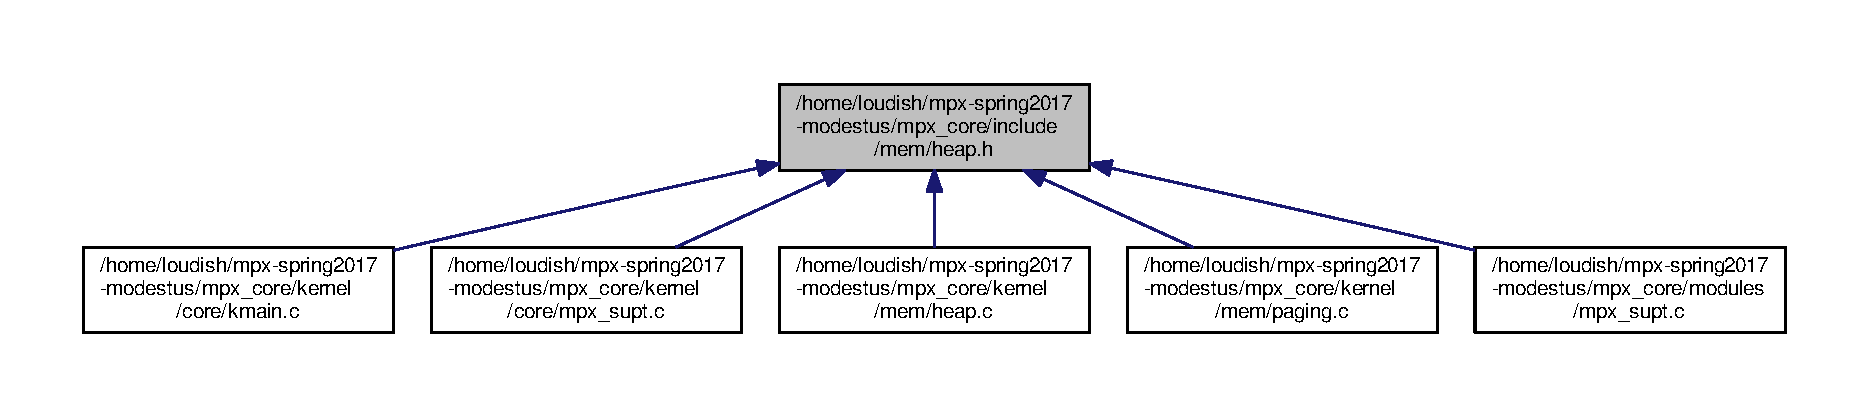
\includegraphics[width=350pt]{heap_8h__dep__incl}
\end{center}
\end{figure}
\subsection*{Data Structures}
\begin{DoxyCompactItemize}
\item 
struct \hyperlink{structheader}{header}
\item 
struct \hyperlink{structfooter}{footer}
\item 
struct \hyperlink{structindex__entry}{index\+\_\+entry}
\item 
struct \hyperlink{structindex__table}{index\+\_\+table}
\item 
struct \hyperlink{structheap}{heap}
\end{DoxyCompactItemize}
\subsection*{Macros}
\begin{DoxyCompactItemize}
\item 
\#define \hyperlink{heap_8h_a032503e76d6f69bc67e99e909c8125da}{T\+A\+B\+L\+E\+\_\+\+S\+I\+ZE}~0x1000
\item 
\#define \hyperlink{heap_8h_a15073b9742f7e29d8174509197eb4ab9}{K\+H\+E\+A\+P\+\_\+\+B\+A\+SE}~0x\+D000000
\item 
\#define \hyperlink{heap_8h_aee52619f74498ad224eb8e4354b89e40}{K\+H\+E\+A\+P\+\_\+\+M\+IN}~0x10000
\item 
\#define \hyperlink{heap_8h_a0f2696767a10e6efffc64e9b459c4ea6}{K\+H\+E\+A\+P\+\_\+\+S\+I\+ZE}~0x1000000
\end{DoxyCompactItemize}
\subsection*{Functions}
\begin{DoxyCompactItemize}
\item 
\hyperlink{system_8h_a757de76cafbcddaac0d1632902fe4cb8}{u32int} \hyperlink{heap_8h_a9bfb8053c2382598ef5b2175f475d49a}{\+\_\+kmalloc} (\hyperlink{system_8h_a757de76cafbcddaac0d1632902fe4cb8}{u32int} size, int align, \hyperlink{system_8h_a757de76cafbcddaac0d1632902fe4cb8}{u32int} $\ast$phys\+\_\+addr)
\item 
\hyperlink{system_8h_a757de76cafbcddaac0d1632902fe4cb8}{u32int} \hyperlink{heap_8h_a15d6a52c5c080c8c7ffc73e336d8e574}{kmalloc} (\hyperlink{system_8h_a757de76cafbcddaac0d1632902fe4cb8}{u32int} size)
\item 
\hyperlink{system_8h_a757de76cafbcddaac0d1632902fe4cb8}{u32int} \hyperlink{heap_8h_aa2a6fb2aa05727dc1e7d72cbc108e63c}{kfree} ()
\item 
void \hyperlink{heap_8h_a755a69ff831b6e23a808dcf4b9944854}{init\+\_\+kheap} ()
\item 
\hyperlink{system_8h_a757de76cafbcddaac0d1632902fe4cb8}{u32int} \hyperlink{heap_8h_a2b1d5a9ba11695605f74fc10cd719af5}{alloc} (\hyperlink{system_8h_a757de76cafbcddaac0d1632902fe4cb8}{u32int} size, \hyperlink{structheap}{heap} $\ast$hp, int align)
\item 
\hyperlink{structheap}{heap} $\ast$ \hyperlink{heap_8h_a686135c02695aef4208f93d4549a15d0}{make\+\_\+heap} (\hyperlink{system_8h_a757de76cafbcddaac0d1632902fe4cb8}{u32int} \hyperlink{tables_8h_ab5763c2b18c825c8b8fba44b2e60ddc1}{base}, \hyperlink{system_8h_a757de76cafbcddaac0d1632902fe4cb8}{u32int} max, \hyperlink{system_8h_a757de76cafbcddaac0d1632902fe4cb8}{u32int} min)
\end{DoxyCompactItemize}


\subsection{Macro Definition Documentation}
\index{heap.\+h@{heap.\+h}!K\+H\+E\+A\+P\+\_\+\+B\+A\+SE@{K\+H\+E\+A\+P\+\_\+\+B\+A\+SE}}
\index{K\+H\+E\+A\+P\+\_\+\+B\+A\+SE@{K\+H\+E\+A\+P\+\_\+\+B\+A\+SE}!heap.\+h@{heap.\+h}}
\subsubsection[{\texorpdfstring{K\+H\+E\+A\+P\+\_\+\+B\+A\+SE}{KHEAP_BASE}}]{\setlength{\rightskip}{0pt plus 5cm}\#define K\+H\+E\+A\+P\+\_\+\+B\+A\+SE~0x\+D000000}\hypertarget{heap_8h_a15073b9742f7e29d8174509197eb4ab9}{}\label{heap_8h_a15073b9742f7e29d8174509197eb4ab9}


Definition at line 6 of file heap.\+h.



Referenced by alloc(), and init\+\_\+paging().

\index{heap.\+h@{heap.\+h}!K\+H\+E\+A\+P\+\_\+\+M\+IN@{K\+H\+E\+A\+P\+\_\+\+M\+IN}}
\index{K\+H\+E\+A\+P\+\_\+\+M\+IN@{K\+H\+E\+A\+P\+\_\+\+M\+IN}!heap.\+h@{heap.\+h}}
\subsubsection[{\texorpdfstring{K\+H\+E\+A\+P\+\_\+\+M\+IN}{KHEAP_MIN}}]{\setlength{\rightskip}{0pt plus 5cm}\#define K\+H\+E\+A\+P\+\_\+\+M\+IN~0x10000}\hypertarget{heap_8h_aee52619f74498ad224eb8e4354b89e40}{}\label{heap_8h_aee52619f74498ad224eb8e4354b89e40}


Definition at line 7 of file heap.\+h.



Referenced by alloc(), and init\+\_\+paging().

\index{heap.\+h@{heap.\+h}!K\+H\+E\+A\+P\+\_\+\+S\+I\+ZE@{K\+H\+E\+A\+P\+\_\+\+S\+I\+ZE}}
\index{K\+H\+E\+A\+P\+\_\+\+S\+I\+ZE@{K\+H\+E\+A\+P\+\_\+\+S\+I\+ZE}!heap.\+h@{heap.\+h}}
\subsubsection[{\texorpdfstring{K\+H\+E\+A\+P\+\_\+\+S\+I\+ZE}{KHEAP_SIZE}}]{\setlength{\rightskip}{0pt plus 5cm}\#define K\+H\+E\+A\+P\+\_\+\+S\+I\+ZE~0x1000000}\hypertarget{heap_8h_a0f2696767a10e6efffc64e9b459c4ea6}{}\label{heap_8h_a0f2696767a10e6efffc64e9b459c4ea6}


Definition at line 8 of file heap.\+h.



Referenced by init\+\_\+paging().

\index{heap.\+h@{heap.\+h}!T\+A\+B\+L\+E\+\_\+\+S\+I\+ZE@{T\+A\+B\+L\+E\+\_\+\+S\+I\+ZE}}
\index{T\+A\+B\+L\+E\+\_\+\+S\+I\+ZE@{T\+A\+B\+L\+E\+\_\+\+S\+I\+ZE}!heap.\+h@{heap.\+h}}
\subsubsection[{\texorpdfstring{T\+A\+B\+L\+E\+\_\+\+S\+I\+ZE}{TABLE_SIZE}}]{\setlength{\rightskip}{0pt plus 5cm}\#define T\+A\+B\+L\+E\+\_\+\+S\+I\+ZE~0x1000}\hypertarget{heap_8h_a032503e76d6f69bc67e99e909c8125da}{}\label{heap_8h_a032503e76d6f69bc67e99e909c8125da}


Definition at line 5 of file heap.\+h.



\subsection{Function Documentation}
\index{heap.\+h@{heap.\+h}!\+\_\+kmalloc@{\+\_\+kmalloc}}
\index{\+\_\+kmalloc@{\+\_\+kmalloc}!heap.\+h@{heap.\+h}}
\subsubsection[{\texorpdfstring{\+\_\+kmalloc(u32int size, int align, u32int $\ast$phys\+\_\+addr)}{_kmalloc(u32int size, int align, u32int *phys_addr)}}]{\setlength{\rightskip}{0pt plus 5cm}{\bf u32int} \+\_\+kmalloc (
\begin{DoxyParamCaption}
\item[{{\bf u32int}}]{size, }
\item[{int}]{align, }
\item[{{\bf u32int} $\ast$}]{phys\+\_\+addr}
\end{DoxyParamCaption}
)}\hypertarget{heap_8h_a9bfb8053c2382598ef5b2175f475d49a}{}\label{heap_8h_a9bfb8053c2382598ef5b2175f475d49a}


Definition at line 24 of file heap.\+c.



References alloc(), page\+\_\+entry\+::frameaddr, get\+\_\+page(), and phys\+\_\+alloc\+\_\+addr.



Referenced by get\+\_\+page(), init\+\_\+paging(), and kmalloc().


\begin{DoxyCode}
25 \{
26   \hyperlink{system_8h_a757de76cafbcddaac0d1632902fe4cb8}{u32int} *addr;
27 
28   \textcolor{comment}{// Allocate on the kernel heap if one has been created}
29   \textcolor{keywordflow}{if} (\hyperlink{heap_8c_a61825456a33b09780a5493c95adcae8a}{kheap} != 0)\{
30     addr = (\hyperlink{system_8h_a757de76cafbcddaac0d1632902fe4cb8}{u32int}*)\hyperlink{heap_8c_a06dae34c7e7c73d518de00212a7c92da}{alloc}(size, \hyperlink{heap_8c_a61825456a33b09780a5493c95adcae8a}{kheap}, page\_align);
31     \textcolor{keywordflow}{if} (phys\_addr)\{
32       \hyperlink{structpage__entry}{page\_entry} *page = \hyperlink{paging_8h_a69b165b3d1adf3aeaae126ca7a5aac3e}{get\_page}((\hyperlink{system_8h_a757de76cafbcddaac0d1632902fe4cb8}{u32int})addr, \hyperlink{heap_8c_a61ce943ba80d9dfab89a826cae9ddc4a}{kdir}, 0);
33       *phys\_addr = (page->\hyperlink{structpage__entry_a68a6dc54a7ab6f7fb1a068476190bf67}{frameaddr}*0x1000) + ((\hyperlink{system_8h_a757de76cafbcddaac0d1632902fe4cb8}{u32int})addr & 0xFFF);
34     \}
35     \textcolor{keywordflow}{return} (\hyperlink{system_8h_a757de76cafbcddaac0d1632902fe4cb8}{u32int})addr;
36   \}
37   \textcolor{comment}{// Else, allocate directly from physical memory}
38   \textcolor{keywordflow}{else} \{
39     \textcolor{keywordflow}{if} (page\_align && (\hyperlink{heap_8c_a6dfa4ef84e115e891b3679e4932b5c49}{phys\_alloc\_addr} & 0xFFFFF000))\{
40       \hyperlink{heap_8c_a6dfa4ef84e115e891b3679e4932b5c49}{phys\_alloc\_addr} &= 0xFFFFF000;
41       \hyperlink{heap_8c_a6dfa4ef84e115e891b3679e4932b5c49}{phys\_alloc\_addr} += 0x1000;
42     \}
43     addr = (\hyperlink{system_8h_a757de76cafbcddaac0d1632902fe4cb8}{u32int}*)\hyperlink{heap_8c_a6dfa4ef84e115e891b3679e4932b5c49}{phys\_alloc\_addr};
44     \textcolor{keywordflow}{if} (phys\_addr)\{
45       *phys\_addr = \hyperlink{heap_8c_a6dfa4ef84e115e891b3679e4932b5c49}{phys\_alloc\_addr};
46     \}
47     \hyperlink{heap_8c_a6dfa4ef84e115e891b3679e4932b5c49}{phys\_alloc\_addr} += size;
48     \textcolor{keywordflow}{return} (\hyperlink{system_8h_a757de76cafbcddaac0d1632902fe4cb8}{u32int})addr;
49   \}
50 \}
\end{DoxyCode}
\index{heap.\+h@{heap.\+h}!alloc@{alloc}}
\index{alloc@{alloc}!heap.\+h@{heap.\+h}}
\subsubsection[{\texorpdfstring{alloc(u32int size, heap $\ast$hp, int align)}{alloc(u32int size, heap *hp, int align)}}]{\setlength{\rightskip}{0pt plus 5cm}{\bf u32int} alloc (
\begin{DoxyParamCaption}
\item[{{\bf u32int}}]{size, }
\item[{{\bf heap} $\ast$}]{hp, }
\item[{int}]{align}
\end{DoxyParamCaption}
)}\hypertarget{heap_8h_a2b1d5a9ba11695605f74fc10cd719af5}{}\label{heap_8h_a2b1d5a9ba11695605f74fc10cd719af5}


Definition at line 57 of file heap.\+c.



References base, K\+H\+E\+A\+P\+\_\+\+B\+A\+SE, K\+H\+E\+A\+P\+\_\+\+M\+IN, no\+\_\+warn, and serial\+\_\+println().



Referenced by \+\_\+kmalloc().


\begin{DoxyCode}
58 \{
59   \hyperlink{system_8h_ab3bb695e7817363c7bdb781f214e83a2}{no\_warn}(size||align||h);
60   \textcolor{keyword}{static} \hyperlink{system_8h_a757de76cafbcddaac0d1632902fe4cb8}{u32int} heap\_addr = \hyperlink{heap_8h_a15073b9742f7e29d8174509197eb4ab9}{KHEAP\_BASE};
61 
62   \hyperlink{system_8h_a757de76cafbcddaac0d1632902fe4cb8}{u32int} \hyperlink{tables_8h_ab5763c2b18c825c8b8fba44b2e60ddc1}{base} = heap\_addr;
63   heap\_addr += size;
64 
65   \textcolor{keywordflow}{if} (heap\_addr > \hyperlink{heap_8h_a15073b9742f7e29d8174509197eb4ab9}{KHEAP\_BASE} + \hyperlink{heap_8h_aee52619f74498ad224eb8e4354b89e40}{KHEAP\_MIN})
66     \hyperlink{serial_8h_a3514f7abff236a4e00a6c46021ce5e22}{serial\_println}(\textcolor{stringliteral}{"Heap is full!"});
67 
68   \textcolor{keywordflow}{return} \hyperlink{tables_8h_ab5763c2b18c825c8b8fba44b2e60ddc1}{base};
69 \}
\end{DoxyCode}
\index{heap.\+h@{heap.\+h}!init\+\_\+kheap@{init\+\_\+kheap}}
\index{init\+\_\+kheap@{init\+\_\+kheap}!heap.\+h@{heap.\+h}}
\subsubsection[{\texorpdfstring{init\+\_\+kheap()}{init_kheap()}}]{\setlength{\rightskip}{0pt plus 5cm}void init\+\_\+kheap (
\begin{DoxyParamCaption}
{}
\end{DoxyParamCaption}
)}\hypertarget{heap_8h_a755a69ff831b6e23a808dcf4b9944854}{}\label{heap_8h_a755a69ff831b6e23a808dcf4b9944854}
\index{heap.\+h@{heap.\+h}!kfree@{kfree}}
\index{kfree@{kfree}!heap.\+h@{heap.\+h}}
\subsubsection[{\texorpdfstring{kfree()}{kfree()}}]{\setlength{\rightskip}{0pt plus 5cm}{\bf u32int} kfree (
\begin{DoxyParamCaption}
{}
\end{DoxyParamCaption}
)}\hypertarget{heap_8h_aa2a6fb2aa05727dc1e7d72cbc108e63c}{}\label{heap_8h_aa2a6fb2aa05727dc1e7d72cbc108e63c}
\index{heap.\+h@{heap.\+h}!kmalloc@{kmalloc}}
\index{kmalloc@{kmalloc}!heap.\+h@{heap.\+h}}
\subsubsection[{\texorpdfstring{kmalloc(u32int size)}{kmalloc(u32int size)}}]{\setlength{\rightskip}{0pt plus 5cm}{\bf u32int} kmalloc (
\begin{DoxyParamCaption}
\item[{{\bf u32int}}]{size}
\end{DoxyParamCaption}
)}\hypertarget{heap_8h_a15d6a52c5c080c8c7ffc73e336d8e574}{}\label{heap_8h_a15d6a52c5c080c8c7ffc73e336d8e574}


Definition at line 52 of file heap.\+c.



References \+\_\+kmalloc().



Referenced by init\+\_\+paging(), make\+\_\+heap(), and sys\+\_\+alloc\+\_\+mem().


\begin{DoxyCode}
53 \{
54   \textcolor{keywordflow}{return} \hyperlink{heap_8c_a014b54e36b61f133f53dd509c461f35e}{\_kmalloc}(size,0,0);
55 \}
\end{DoxyCode}
\index{heap.\+h@{heap.\+h}!make\+\_\+heap@{make\+\_\+heap}}
\index{make\+\_\+heap@{make\+\_\+heap}!heap.\+h@{heap.\+h}}
\subsubsection[{\texorpdfstring{make\+\_\+heap(u32int base, u32int max, u32int min)}{make_heap(u32int base, u32int max, u32int min)}}]{\setlength{\rightskip}{0pt plus 5cm}{\bf heap}$\ast$ make\+\_\+heap (
\begin{DoxyParamCaption}
\item[{{\bf u32int}}]{base, }
\item[{{\bf u32int}}]{max, }
\item[{{\bf u32int}}]{min}
\end{DoxyParamCaption}
)}\hypertarget{heap_8h_a686135c02695aef4208f93d4549a15d0}{}\label{heap_8h_a686135c02695aef4208f93d4549a15d0}


Definition at line 71 of file heap.\+c.



References kmalloc(), and no\+\_\+warn.



Referenced by init\+\_\+paging().


\begin{DoxyCode}
72 \{  
73   \hyperlink{system_8h_ab3bb695e7817363c7bdb781f214e83a2}{no\_warn}(\hyperlink{tables_8h_ab5763c2b18c825c8b8fba44b2e60ddc1}{base}||max||min);
74   \textcolor{keywordflow}{return} (\hyperlink{structheap}{heap}*)\hyperlink{heap_8c_a15d6a52c5c080c8c7ffc73e336d8e574}{kmalloc}(\textcolor{keyword}{sizeof}(\hyperlink{structheap}{heap}));
75 \}
\end{DoxyCode}

\hypertarget{paging_8h}{}\section{/home/loudish/mpx-\/spring2017-\/modestus/mpx\+\_\+core/include/mem/paging.h File Reference}
\label{paging_8h}\index{/home/loudish/mpx-\/spring2017-\/modestus/mpx\+\_\+core/include/mem/paging.\+h@{/home/loudish/mpx-\/spring2017-\/modestus/mpx\+\_\+core/include/mem/paging.\+h}}
{\ttfamily \#include $<$system.\+h$>$}\\*
Include dependency graph for paging.\+h\+:\nopagebreak
\begin{figure}[H]
\begin{center}
\leavevmode
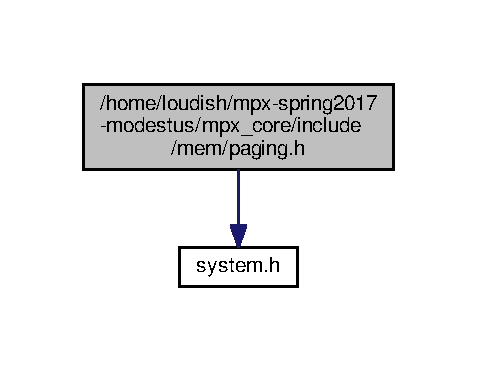
\includegraphics[width=229pt]{paging_8h__incl}
\end{center}
\end{figure}
This graph shows which files directly or indirectly include this file\+:\nopagebreak
\begin{figure}[H]
\begin{center}
\leavevmode
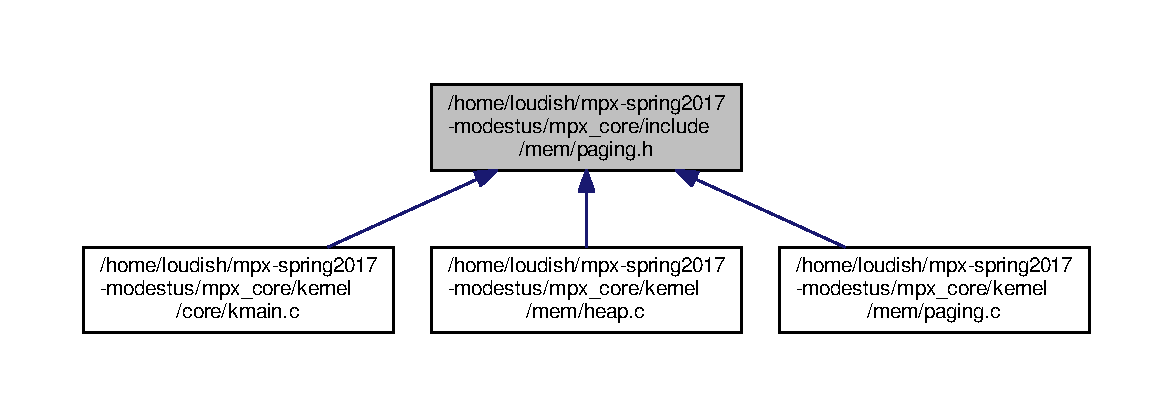
\includegraphics[width=350pt]{paging_8h__dep__incl}
\end{center}
\end{figure}
\subsection*{Data Structures}
\begin{DoxyCompactItemize}
\item 
struct \hyperlink{structpage__entry}{page\+\_\+entry}
\item 
struct \hyperlink{structpage__table}{page\+\_\+table}
\item 
struct \hyperlink{structpage__dir}{page\+\_\+dir}
\end{DoxyCompactItemize}
\subsection*{Macros}
\begin{DoxyCompactItemize}
\item 
\#define \hyperlink{paging_8h_a7d467c1d283fdfa1f2081ba1e0d01b6e}{P\+A\+G\+E\+\_\+\+S\+I\+ZE}~0x1000
\end{DoxyCompactItemize}
\subsection*{Functions}
\begin{DoxyCompactItemize}
\item 
void \hyperlink{paging_8h_a70101fc152ff58caafbe36ab391a9a68}{set\+\_\+bit} (\hyperlink{system_8h_a757de76cafbcddaac0d1632902fe4cb8}{u32int} addr)
\item 
void \hyperlink{paging_8h_adcef508c82c20a032508f871e79e1b92}{clear\+\_\+bit} (\hyperlink{system_8h_a757de76cafbcddaac0d1632902fe4cb8}{u32int} addr)
\item 
\hyperlink{system_8h_a757de76cafbcddaac0d1632902fe4cb8}{u32int} \hyperlink{paging_8h_a317b4797bc81f65bd01cfa190800ecdd}{get\+\_\+bit} (\hyperlink{system_8h_a757de76cafbcddaac0d1632902fe4cb8}{u32int} addr)
\item 
\hyperlink{system_8h_a757de76cafbcddaac0d1632902fe4cb8}{u32int} \hyperlink{paging_8h_acb3c25257061521382c7ba900c1c1ab4}{first\+\_\+free} ()
\item 
void \hyperlink{paging_8h_a919b727f386797a8b9d8eceb5c4e7313}{init\+\_\+paging} ()
\item 
void \hyperlink{paging_8h_a3affceba4cd194e1c516404c14abbe7c}{load\+\_\+page\+\_\+dir} (\hyperlink{structpage__dir}{page\+\_\+dir} $\ast$new\+\_\+page\+\_\+dir)
\item 
\hyperlink{structpage__entry}{page\+\_\+entry} $\ast$ \hyperlink{paging_8h_a69b165b3d1adf3aeaae126ca7a5aac3e}{get\+\_\+page} (\hyperlink{system_8h_a757de76cafbcddaac0d1632902fe4cb8}{u32int} addr, \hyperlink{structpage__dir}{page\+\_\+dir} $\ast$dir, int make\+\_\+table)
\item 
void \hyperlink{paging_8h_a04bce9da2c1d7c59f6efd8e4d9b54db7}{new\+\_\+frame} (\hyperlink{structpage__entry}{page\+\_\+entry} $\ast$page)
\end{DoxyCompactItemize}


\subsection{Macro Definition Documentation}
\index{paging.\+h@{paging.\+h}!P\+A\+G\+E\+\_\+\+S\+I\+ZE@{P\+A\+G\+E\+\_\+\+S\+I\+ZE}}
\index{P\+A\+G\+E\+\_\+\+S\+I\+ZE@{P\+A\+G\+E\+\_\+\+S\+I\+ZE}!paging.\+h@{paging.\+h}}
\subsubsection[{\texorpdfstring{P\+A\+G\+E\+\_\+\+S\+I\+ZE}{PAGE_SIZE}}]{\setlength{\rightskip}{0pt plus 5cm}\#define P\+A\+G\+E\+\_\+\+S\+I\+ZE~0x1000}\hypertarget{paging_8h_a7d467c1d283fdfa1f2081ba1e0d01b6e}{}\label{paging_8h_a7d467c1d283fdfa1f2081ba1e0d01b6e}


Definition at line 6 of file paging.\+h.



Referenced by init\+\_\+paging().



\subsection{Function Documentation}
\index{paging.\+h@{paging.\+h}!clear\+\_\+bit@{clear\+\_\+bit}}
\index{clear\+\_\+bit@{clear\+\_\+bit}!paging.\+h@{paging.\+h}}
\subsubsection[{\texorpdfstring{clear\+\_\+bit(u32int addr)}{clear_bit(u32int addr)}}]{\setlength{\rightskip}{0pt plus 5cm}void clear\+\_\+bit (
\begin{DoxyParamCaption}
\item[{{\bf u32int}}]{addr}
\end{DoxyParamCaption}
)}\hypertarget{paging_8h_adcef508c82c20a032508f871e79e1b92}{}\label{paging_8h_adcef508c82c20a032508f871e79e1b92}


Definition at line 44 of file paging.\+c.



References frames, and page\+\_\+size.


\begin{DoxyCode}
45 \{
46   \hyperlink{system_8h_a757de76cafbcddaac0d1632902fe4cb8}{u32int} frame  = addr/\hyperlink{paging_8c_a1cc472551ec40b65eef931fde01054e7}{page\_size};
47   \hyperlink{system_8h_a757de76cafbcddaac0d1632902fe4cb8}{u32int} index  = frame/32;
48   \hyperlink{system_8h_a757de76cafbcddaac0d1632902fe4cb8}{u32int} offset = frame%32;
49   \hyperlink{paging_8c_a76492529572a1a20a06076ac40d66b29}{frames}[index] &= ~(1 << offset);
50 \}
\end{DoxyCode}
\index{paging.\+h@{paging.\+h}!first\+\_\+free@{first\+\_\+free}}
\index{first\+\_\+free@{first\+\_\+free}!paging.\+h@{paging.\+h}}
\subsubsection[{\texorpdfstring{first\+\_\+free()}{first_free()}}]{\setlength{\rightskip}{0pt plus 5cm}{\bf u32int} first\+\_\+free (
\begin{DoxyParamCaption}
{}
\end{DoxyParamCaption}
)}\hypertarget{paging_8h_acb3c25257061521382c7ba900c1c1ab4}{}\label{paging_8h_acb3c25257061521382c7ba900c1c1ab4}
\index{paging.\+h@{paging.\+h}!get\+\_\+bit@{get\+\_\+bit}}
\index{get\+\_\+bit@{get\+\_\+bit}!paging.\+h@{paging.\+h}}
\subsubsection[{\texorpdfstring{get\+\_\+bit(u32int addr)}{get_bit(u32int addr)}}]{\setlength{\rightskip}{0pt plus 5cm}{\bf u32int} get\+\_\+bit (
\begin{DoxyParamCaption}
\item[{{\bf u32int}}]{addr}
\end{DoxyParamCaption}
)}\hypertarget{paging_8h_a317b4797bc81f65bd01cfa190800ecdd}{}\label{paging_8h_a317b4797bc81f65bd01cfa190800ecdd}


Definition at line 56 of file paging.\+c.



References frames, and page\+\_\+size.


\begin{DoxyCode}
57 \{
58   \hyperlink{system_8h_a757de76cafbcddaac0d1632902fe4cb8}{u32int} frame  = addr/\hyperlink{paging_8c_a1cc472551ec40b65eef931fde01054e7}{page\_size};
59   \hyperlink{system_8h_a757de76cafbcddaac0d1632902fe4cb8}{u32int} index  = frame/32;
60   \hyperlink{system_8h_a757de76cafbcddaac0d1632902fe4cb8}{u32int} offset = frame%32;
61   \textcolor{keywordflow}{return} (\hyperlink{paging_8c_a76492529572a1a20a06076ac40d66b29}{frames}[index] & (1 << offset));  
62 \}
\end{DoxyCode}
\index{paging.\+h@{paging.\+h}!get\+\_\+page@{get\+\_\+page}}
\index{get\+\_\+page@{get\+\_\+page}!paging.\+h@{paging.\+h}}
\subsubsection[{\texorpdfstring{get\+\_\+page(u32int addr, page\+\_\+dir $\ast$dir, int make\+\_\+table)}{get_page(u32int addr, page_dir *dir, int make_table)}}]{\setlength{\rightskip}{0pt plus 5cm}{\bf page\+\_\+entry}$\ast$ get\+\_\+page (
\begin{DoxyParamCaption}
\item[{{\bf u32int}}]{addr, }
\item[{{\bf page\+\_\+dir} $\ast$}]{dir, }
\item[{int}]{make\+\_\+table}
\end{DoxyParamCaption}
)}\hypertarget{paging_8h_a69b165b3d1adf3aeaae126ca7a5aac3e}{}\label{paging_8h_a69b165b3d1adf3aeaae126ca7a5aac3e}


Definition at line 85 of file paging.\+c.



References \+\_\+kmalloc(), page\+\_\+size, page\+\_\+table\+::pages, page\+\_\+dir\+::tables, and page\+\_\+dir\+::tables\+\_\+phys.



Referenced by \+\_\+kmalloc(), and init\+\_\+paging().


\begin{DoxyCode}
86 \{
87   \hyperlink{system_8h_a757de76cafbcddaac0d1632902fe4cb8}{u32int} phys\_addr;
88   \hyperlink{system_8h_a757de76cafbcddaac0d1632902fe4cb8}{u32int} index = addr / \hyperlink{paging_8c_a1cc472551ec40b65eef931fde01054e7}{page\_size} / 1024;
89   \hyperlink{system_8h_a757de76cafbcddaac0d1632902fe4cb8}{u32int} offset = addr / \hyperlink{paging_8c_a1cc472551ec40b65eef931fde01054e7}{page\_size} % 1024;
90   
91   \textcolor{comment}{//return it if it exists}
92   \textcolor{keywordflow}{if} (dir->\hyperlink{structpage__dir_ac89434e3fccabfe9481ea77fdda82faf}{tables}[index])
93     \textcolor{keywordflow}{return} &dir->\hyperlink{structpage__dir_ac89434e3fccabfe9481ea77fdda82faf}{tables}[index]->\hyperlink{structpage__table_aa066e0fa847ce2fafb6a2feddfa340ff}{pages}[offset];
94   
95   \textcolor{comment}{//create it}
96   \textcolor{keywordflow}{else} \textcolor{keywordflow}{if} (make\_table)\{
97     dir->\hyperlink{structpage__dir_ac89434e3fccabfe9481ea77fdda82faf}{tables}[index] = (\hyperlink{structpage__table}{page\_table}*)\hyperlink{heap_8h_a9bfb8053c2382598ef5b2175f475d49a}{\_kmalloc}(\textcolor{keyword}{sizeof}(
      \hyperlink{structpage__table}{page\_table}), 1, &phys\_addr);
98     dir->\hyperlink{structpage__dir_a7336b695acaf516613dda626129129d0}{tables\_phys}[index] = phys\_addr | 0x7; \textcolor{comment}{//enable present, writable}
99     \textcolor{keywordflow}{return} &dir->\hyperlink{structpage__dir_ac89434e3fccabfe9481ea77fdda82faf}{tables}[index]->\hyperlink{structpage__table_aa066e0fa847ce2fafb6a2feddfa340ff}{pages}[offset];
100   \}
101   \textcolor{keywordflow}{else} \textcolor{keywordflow}{return} 0;
102 \}
\end{DoxyCode}
\index{paging.\+h@{paging.\+h}!init\+\_\+paging@{init\+\_\+paging}}
\index{init\+\_\+paging@{init\+\_\+paging}!paging.\+h@{paging.\+h}}
\subsubsection[{\texorpdfstring{init\+\_\+paging()}{init_paging()}}]{\setlength{\rightskip}{0pt plus 5cm}void init\+\_\+paging (
\begin{DoxyParamCaption}
{}
\end{DoxyParamCaption}
)}\hypertarget{paging_8h_a919b727f386797a8b9d8eceb5c4e7313}{}\label{paging_8h_a919b727f386797a8b9d8eceb5c4e7313}


Definition at line 111 of file paging.\+c.



References \+\_\+kmalloc(), frames, get\+\_\+page(), K\+H\+E\+A\+P\+\_\+\+B\+A\+SE, K\+H\+E\+A\+P\+\_\+\+M\+IN, K\+H\+E\+A\+P\+\_\+\+S\+I\+ZE, kmalloc(), load\+\_\+page\+\_\+dir(), make\+\_\+heap(), mem\+\_\+size, memset(), new\+\_\+frame(), nframes, P\+A\+G\+E\+\_\+\+S\+I\+ZE, page\+\_\+size, and phys\+\_\+alloc\+\_\+addr.



Referenced by kmain().


\begin{DoxyCode}
112 \{
113   \textcolor{comment}{//create frame bitmap}
114   \hyperlink{paging_8c_abf36580d5618820f15388083c9313e60}{nframes} = (\hyperlink{system_8h_a757de76cafbcddaac0d1632902fe4cb8}{u32int})(\hyperlink{paging_8c_abf8475f59bfb67fac4b6b5a254dfe56d}{mem\_size}/\hyperlink{paging_8c_a1cc472551ec40b65eef931fde01054e7}{page\_size});
115   \hyperlink{paging_8c_a76492529572a1a20a06076ac40d66b29}{frames} = (\hyperlink{system_8h_a757de76cafbcddaac0d1632902fe4cb8}{u32int}*)\hyperlink{heap_8h_a15d6a52c5c080c8c7ffc73e336d8e574}{kmalloc}(\hyperlink{paging_8c_abf36580d5618820f15388083c9313e60}{nframes}/32);
116   \hyperlink{string_8h_ace6ee45c30e71865e6eb635200379db9}{memset}(\hyperlink{paging_8c_a76492529572a1a20a06076ac40d66b29}{frames}, 0, \hyperlink{paging_8c_abf36580d5618820f15388083c9313e60}{nframes}/32);
117 
118   \textcolor{comment}{//create kernel directory}
119   \hyperlink{paging_8c_a61ce943ba80d9dfab89a826cae9ddc4a}{kdir} = (\hyperlink{structpage__dir}{page\_dir}*)\hyperlink{heap_8h_a9bfb8053c2382598ef5b2175f475d49a}{\_kmalloc}(\textcolor{keyword}{sizeof}(\hyperlink{structpage__dir}{page\_dir}), 1, 0); \textcolor{comment}{//page aligned}
120   \hyperlink{string_8h_ace6ee45c30e71865e6eb635200379db9}{memset}(\hyperlink{paging_8c_a61ce943ba80d9dfab89a826cae9ddc4a}{kdir}, 0, \textcolor{keyword}{sizeof}(\hyperlink{structpage__dir}{page\_dir}));
121 
122   \textcolor{comment}{//get pages for kernel heap}
123   \hyperlink{system_8h_a757de76cafbcddaac0d1632902fe4cb8}{u32int} i = 0x0;
124   \textcolor{keywordflow}{for}(i=\hyperlink{heap_8h_a15073b9742f7e29d8174509197eb4ab9}{KHEAP\_BASE}; i<(\hyperlink{heap_8h_a15073b9742f7e29d8174509197eb4ab9}{KHEAP\_BASE}+\hyperlink{heap_8h_aee52619f74498ad224eb8e4354b89e40}{KHEAP\_MIN}); i+=1)\{
125     \hyperlink{paging_8c_a69b165b3d1adf3aeaae126ca7a5aac3e}{get\_page}(i,\hyperlink{paging_8c_a61ce943ba80d9dfab89a826cae9ddc4a}{kdir},1);
126   \}
127 
128   \textcolor{comment}{//perform identity mapping of used memory}
129   \textcolor{comment}{//note: placement\_addr gets incremented in get\_page,}
130   \textcolor{comment}{//so we're mapping the first frames as well}
131   i = 0x0;
132   \textcolor{keywordflow}{while} (i < (\hyperlink{paging_8c_a6dfa4ef84e115e891b3679e4932b5c49}{phys\_alloc\_addr}+0x10000))\{
133     \hyperlink{paging_8c_a04bce9da2c1d7c59f6efd8e4d9b54db7}{new\_frame}(\hyperlink{paging_8c_a69b165b3d1adf3aeaae126ca7a5aac3e}{get\_page}(i,\hyperlink{paging_8c_a61ce943ba80d9dfab89a826cae9ddc4a}{kdir},1));
134     i += \hyperlink{paging_8c_a1cc472551ec40b65eef931fde01054e7}{page\_size};
135   \}
136 
137   \textcolor{comment}{//allocate heap frames now that the placement addr has increased.}
138   \textcolor{comment}{//placement addr increases here for heap}
139   \textcolor{keywordflow}{for}(i=\hyperlink{heap_8h_a15073b9742f7e29d8174509197eb4ab9}{KHEAP\_BASE}; i<(\hyperlink{heap_8h_a15073b9742f7e29d8174509197eb4ab9}{KHEAP\_BASE}+\hyperlink{heap_8h_aee52619f74498ad224eb8e4354b89e40}{KHEAP\_MIN});i+=
      \hyperlink{paging_8h_a7d467c1d283fdfa1f2081ba1e0d01b6e}{PAGE\_SIZE})\{
140     \hyperlink{paging_8c_a04bce9da2c1d7c59f6efd8e4d9b54db7}{new\_frame}(\hyperlink{paging_8c_a69b165b3d1adf3aeaae126ca7a5aac3e}{get\_page}(i,\hyperlink{paging_8c_a61ce943ba80d9dfab89a826cae9ddc4a}{kdir},1));
141   \}
142 
143   \textcolor{comment}{//load the kernel page directory; enable paging}
144   \hyperlink{paging_8c_a31e6c585cbda542534f1b0fc83e40689}{load\_page\_dir}(\hyperlink{paging_8c_a61ce943ba80d9dfab89a826cae9ddc4a}{kdir});
145 
146   \textcolor{comment}{//setup the kernel heap}
147   \hyperlink{paging_8c_a61825456a33b09780a5493c95adcae8a}{kheap} = \hyperlink{heap_8h_a686135c02695aef4208f93d4549a15d0}{make\_heap}(\hyperlink{heap_8h_a15073b9742f7e29d8174509197eb4ab9}{KHEAP\_BASE}, \hyperlink{heap_8h_a0f2696767a10e6efffc64e9b459c4ea6}{KHEAP\_SIZE}, 
      \hyperlink{heap_8h_a15073b9742f7e29d8174509197eb4ab9}{KHEAP\_BASE}+\hyperlink{heap_8h_aee52619f74498ad224eb8e4354b89e40}{KHEAP\_MIN});
148 \}
\end{DoxyCode}
\index{paging.\+h@{paging.\+h}!load\+\_\+page\+\_\+dir@{load\+\_\+page\+\_\+dir}}
\index{load\+\_\+page\+\_\+dir@{load\+\_\+page\+\_\+dir}!paging.\+h@{paging.\+h}}
\subsubsection[{\texorpdfstring{load\+\_\+page\+\_\+dir(page\+\_\+dir $\ast$new\+\_\+page\+\_\+dir)}{load_page_dir(page_dir *new_page_dir)}}]{\setlength{\rightskip}{0pt plus 5cm}void load\+\_\+page\+\_\+dir (
\begin{DoxyParamCaption}
\item[{{\bf page\+\_\+dir} $\ast$}]{new\+\_\+page\+\_\+dir}
\end{DoxyParamCaption}
)}\hypertarget{paging_8h_a3affceba4cd194e1c516404c14abbe7c}{}\label{paging_8h_a3affceba4cd194e1c516404c14abbe7c}


Definition at line 158 of file paging.\+c.



References page\+\_\+dir\+::tables\+\_\+phys.



Referenced by init\+\_\+paging().


\begin{DoxyCode}
159 \{
160   \hyperlink{paging_8c_af7da380833e92d5c7d3c3db41484713b}{cdir} = new\_dir;
161   \textcolor{keyword}{asm} \textcolor{keyword}{volatile} (\textcolor{stringliteral}{"mov %0,%%cr3"}:: \textcolor{stringliteral}{"b"}(&\hyperlink{paging_8c_af7da380833e92d5c7d3c3db41484713b}{cdir}->\hyperlink{structpage__dir_a7336b695acaf516613dda626129129d0}{tables\_phys}[0]));
162   \hyperlink{system_8h_a757de76cafbcddaac0d1632902fe4cb8}{u32int} cr0;
163   \textcolor{keyword}{asm} \textcolor{keyword}{volatile} (\textcolor{stringliteral}{"mov %%cr0,%0"}: \textcolor{stringliteral}{"=b"}(cr0));
164   cr0 |= 0x80000000;
165   \textcolor{keyword}{asm} \textcolor{keyword}{volatile} (\textcolor{stringliteral}{"mov %0,%%cr0"}:: \textcolor{stringliteral}{"b"}(cr0));
166 \}
\end{DoxyCode}
\index{paging.\+h@{paging.\+h}!new\+\_\+frame@{new\+\_\+frame}}
\index{new\+\_\+frame@{new\+\_\+frame}!paging.\+h@{paging.\+h}}
\subsubsection[{\texorpdfstring{new\+\_\+frame(page\+\_\+entry $\ast$page)}{new_frame(page_entry *page)}}]{\setlength{\rightskip}{0pt plus 5cm}void new\+\_\+frame (
\begin{DoxyParamCaption}
\item[{{\bf page\+\_\+entry} $\ast$}]{page}
\end{DoxyParamCaption}
)}\hypertarget{paging_8h_a04bce9da2c1d7c59f6efd8e4d9b54db7}{}\label{paging_8h_a04bce9da2c1d7c59f6efd8e4d9b54db7}


Definition at line 173 of file paging.\+c.



References find\+\_\+free(), page\+\_\+entry\+::frameaddr, kpanic(), page\+\_\+size, page\+\_\+entry\+::present, set\+\_\+bit(), page\+\_\+entry\+::usermode, and page\+\_\+entry\+::writeable.



Referenced by init\+\_\+paging().


\begin{DoxyCode}
174 \{
175   \hyperlink{system_8h_a757de76cafbcddaac0d1632902fe4cb8}{u32int} index;
176   \textcolor{keywordflow}{if} (page->\hyperlink{structpage__entry_a68a6dc54a7ab6f7fb1a068476190bf67}{frameaddr} != 0) \textcolor{keywordflow}{return};
177   \textcolor{keywordflow}{if} ( (\hyperlink{system_8h_a757de76cafbcddaac0d1632902fe4cb8}{u32int})(-1) == (index=\hyperlink{paging_8c_abe201f9294ab23125146fff36fe95187}{find\_free}()) ) \hyperlink{system_8h_aff8473f901d828d76d3548130731c41d}{kpanic}(\textcolor{stringliteral}{"Out of memory"});
178   
179   \textcolor{comment}{//mark a frame as in-use}
180   \hyperlink{paging_8c_a70101fc152ff58caafbe36ab391a9a68}{set\_bit}(index*\hyperlink{paging_8c_a1cc472551ec40b65eef931fde01054e7}{page\_size});
181   page->\hyperlink{structpage__entry_a34148a94af9bfabbb8c4f00f9865dfee}{present}   = 1;
182   page->\hyperlink{structpage__entry_a68a6dc54a7ab6f7fb1a068476190bf67}{frameaddr} = index;
183   page->\hyperlink{structpage__entry_a2ea8d7684fe45772b6acba70d46e41d9}{writeable} = 1;
184   page->\hyperlink{structpage__entry_a2beafd3900a1f36f09af9c35a9a14f18}{usermode}  = 0;
185 \}
\end{DoxyCode}
\index{paging.\+h@{paging.\+h}!set\+\_\+bit@{set\+\_\+bit}}
\index{set\+\_\+bit@{set\+\_\+bit}!paging.\+h@{paging.\+h}}
\subsubsection[{\texorpdfstring{set\+\_\+bit(u32int addr)}{set_bit(u32int addr)}}]{\setlength{\rightskip}{0pt plus 5cm}void set\+\_\+bit (
\begin{DoxyParamCaption}
\item[{{\bf u32int}}]{addr}
\end{DoxyParamCaption}
)}\hypertarget{paging_8h_a70101fc152ff58caafbe36ab391a9a68}{}\label{paging_8h_a70101fc152ff58caafbe36ab391a9a68}


Definition at line 32 of file paging.\+c.



References frames, and page\+\_\+size.



Referenced by new\+\_\+frame().


\begin{DoxyCode}
33 \{
34   \hyperlink{system_8h_a757de76cafbcddaac0d1632902fe4cb8}{u32int} frame  = addr/\hyperlink{paging_8c_a1cc472551ec40b65eef931fde01054e7}{page\_size};
35   \hyperlink{system_8h_a757de76cafbcddaac0d1632902fe4cb8}{u32int} index  = frame/32;
36   \hyperlink{system_8h_a757de76cafbcddaac0d1632902fe4cb8}{u32int} offset = frame%32;
37   \hyperlink{paging_8c_a76492529572a1a20a06076ac40d66b29}{frames}[index] |= (1 << offset);
38 \}
\end{DoxyCode}

\hypertarget{string_8h}{}\section{/home/loudish/mpx-\/spring2017-\/modestus/mpx\+\_\+core/include/string.h File Reference}
\label{string_8h}\index{/home/loudish/mpx-\/spring2017-\/modestus/mpx\+\_\+core/include/string.\+h@{/home/loudish/mpx-\/spring2017-\/modestus/mpx\+\_\+core/include/string.\+h}}
{\ttfamily \#include $<$system.\+h$>$}\\*
{\ttfamily \#include $<$arg\+\_\+list.\+h$>$}\\*
{\ttfamily \#include $<$core/serial.\+h$>$}\\*
Include dependency graph for string.\+h\+:\nopagebreak
\begin{figure}[H]
\begin{center}
\leavevmode
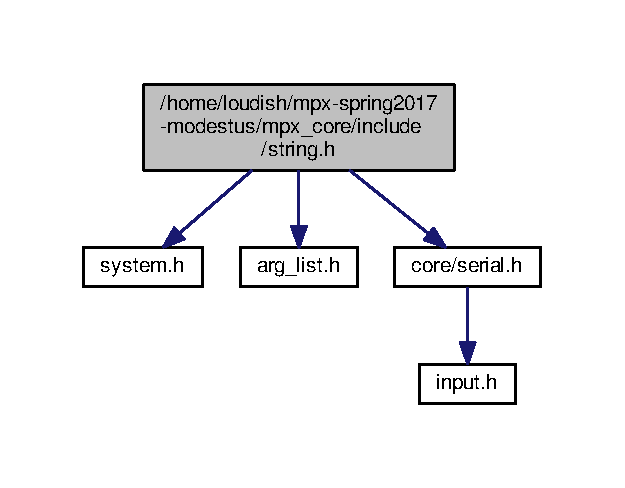
\includegraphics[width=300pt]{string_8h__incl}
\end{center}
\end{figure}
This graph shows which files directly or indirectly include this file\+:\nopagebreak
\begin{figure}[H]
\begin{center}
\leavevmode
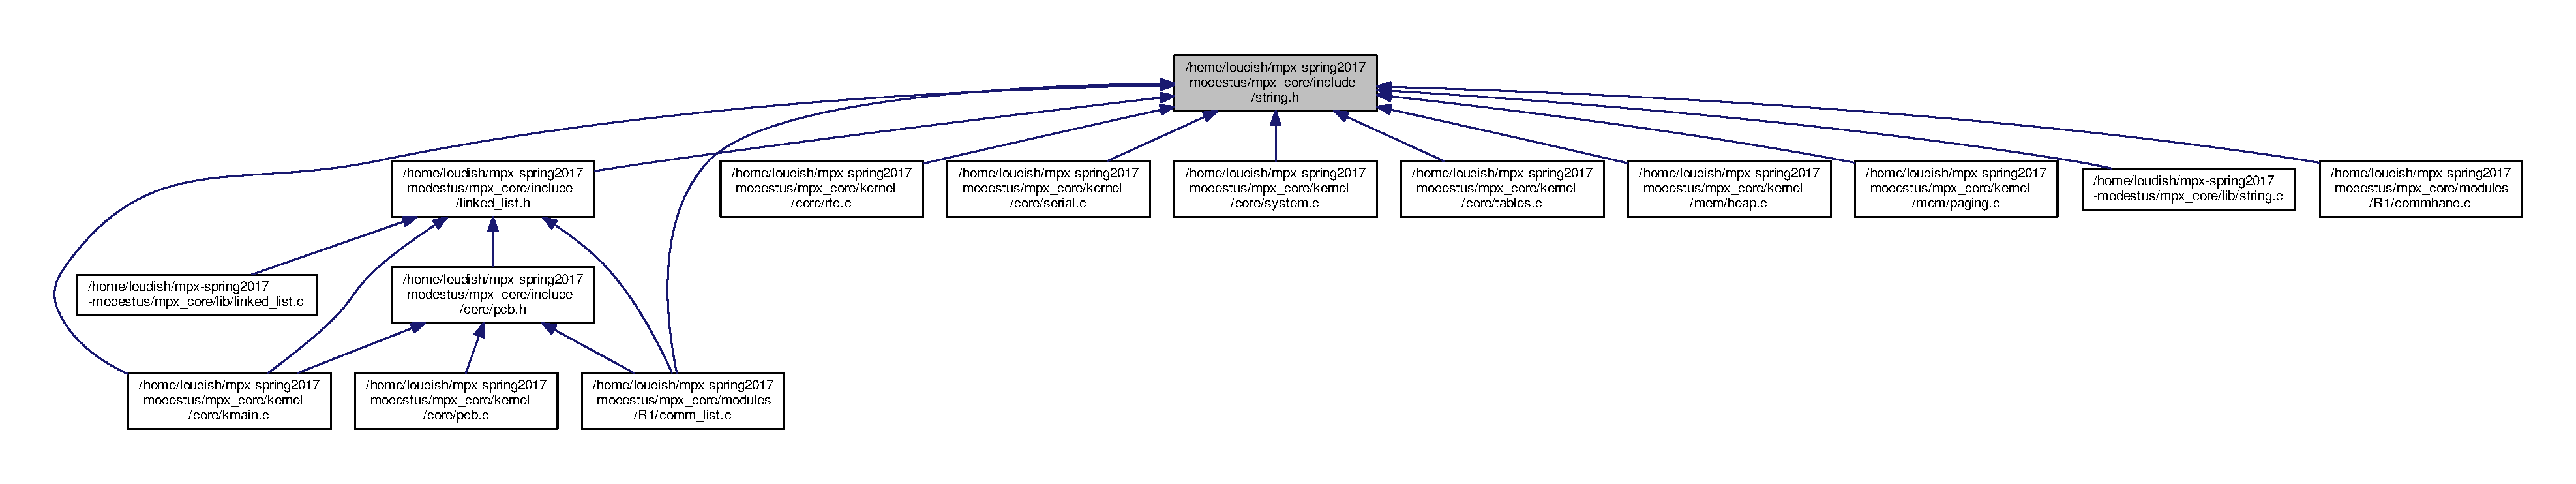
\includegraphics[width=350pt]{string_8h__dep__incl}
\end{center}
\end{figure}
\subsection*{Macros}
\begin{DoxyCompactItemize}
\item 
\#define \hyperlink{string_8h_a0f459d16901ef591acaafa4b67fd4be5}{printf}(format, ...)
\begin{DoxyCompactList}\small\item\em printf is simply a wrapper macro around sprintf with built in terminal print builtin needs to be a macro to pass on varidic function args. Uses the C Language B\+U\+I\+L\+T-\/\+IT macro to use marco varidic functionability. \end{DoxyCompactList}\end{DoxyCompactItemize}
\subsection*{Functions}
\begin{DoxyCompactItemize}
\item 
int \hyperlink{string_8h_a0f3d37d605e9e6d4fc1853ff9d4b91bf}{isspace} (const char $\ast$c)
\begin{DoxyCompactList}\small\item\em isspace Determines if a character is a whitespace. \end{DoxyCompactList}\item 
void $\ast$ \hyperlink{string_8h_ace6ee45c30e71865e6eb635200379db9}{memset} (void $\ast$s, int c, \hyperlink{system_8h_a7c94ea6f8948649f8d181ae55911eeaf}{size\+\_\+t} n)
\begin{DoxyCompactList}\small\item\em memset Set a region of memory. \end{DoxyCompactList}\item 
char $\ast$ \hyperlink{string_8h_a1eb9cae61e6a6282c28dbc298ef7297e}{strcpy} (char $\ast$s1, const char $\ast$s2)
\begin{DoxyCompactList}\small\item\em strcpy copies one string to another string \end{DoxyCompactList}\item 
char $\ast$ \hyperlink{string_8h_a8908188ae9fc2f05d993257ef001d553}{strcat} (char $\ast$s1, const char $\ast$s2)
\begin{DoxyCompactList}\small\item\em strcat concatenates the contents of one string onto another. \end{DoxyCompactList}\item 
int \hyperlink{string_8h_a2dee044e4e667b5b789b493abd21cfa4}{strlen} (const char $\ast$s)
\begin{DoxyCompactList}\small\item\em strlen returns the length of a string \end{DoxyCompactList}\item 
int \hyperlink{string_8h_a11bd144d7d44914099a3aeddf1c8567d}{strcmp} (const char $\ast$s1, const char $\ast$s2)
\begin{DoxyCompactList}\small\item\em strcmp compares two strings. \end{DoxyCompactList}\item 
char $\ast$ \hyperlink{string_8h_af1a867dcea42fc1215d0eddf19283ef3}{strtok} (char $\ast$s1, const char $\ast$s2)
\begin{DoxyCompactList}\small\item\em strtok Split string into tokens. \end{DoxyCompactList}\item 
int \hyperlink{string_8h_a30670a60464f77af17dfb353353d6df8}{atoi} (const char $\ast$s)
\begin{DoxyCompactList}\small\item\em atoi converts and A\+S\+C\+II string to an integer \end{DoxyCompactList}\item 
int \hyperlink{string_8h_a397a240a4a5dc802bd2ba2054d25ae15}{int\+ToS} (const int $\ast$const i, char $\ast$buf, int buf\+Length)
\begin{DoxyCompactList}\small\item\em int\+ToS converts a signed integer to string \end{DoxyCompactList}\item 
char \hyperlink{string_8h_aca5e96bcd4ba56fb4d7ac75160f2161c}{is\+\_\+conversion\+\_\+specifier} (char c)
\begin{DoxyCompactList}\small\item\em is\+\_\+conversion\+\_\+specifier checks to see if the character is one of the standard printf formats \end{DoxyCompactList}\item 
int \hyperlink{string_8h_a1153bdbe1c0758a66d46bdefa2eb755d}{isnum} (const char c)
\begin{DoxyCompactList}\small\item\em isnum inline helper function to check if a character is represents an ascii number \end{DoxyCompactList}\item 
int \hyperlink{string_8h_ae9cac82f3293a00d8ec8705a3fc5cf64}{sprintf} (char $\ast$str, int buf\+Length, const char $\ast$format,...) \hyperlink{string_8c_a4adae2826c898e6fded351cfebc561b4}{\+\_\+\+\_\+attribute\+\_\+\+\_\+}((format(\hyperlink{string_8h_a0f459d16901ef591acaafa4b67fd4be5}{printf}
\begin{DoxyCompactList}\small\item\em sprintf print with format to specified string buffer \end{DoxyCompactList}\end{DoxyCompactItemize}


\subsection{Macro Definition Documentation}
\index{string.\+h@{string.\+h}!printf@{printf}}
\index{printf@{printf}!string.\+h@{string.\+h}}
\subsubsection[{\texorpdfstring{printf}{printf}}]{\setlength{\rightskip}{0pt plus 5cm}\#define printf(
\begin{DoxyParamCaption}
\item[{}]{format, }
\item[{}]{...}
\end{DoxyParamCaption}
)}\hypertarget{string_8h_a0f459d16901ef591acaafa4b67fd4be5}{}\label{string_8h_a0f459d16901ef591acaafa4b67fd4be5}
{\bfseries Value\+:}
\begin{DoxyCode}
\{ \(\backslash\)
    char buf[500]; \hyperlink{string_8h_ae9cac82f3293a00d8ec8705a3fc5cf64}{\(\backslash\)}
\hyperlink{string_8h_ae9cac82f3293a00d8ec8705a3fc5cf64}{    sprintf}(buf, 500, format, \_\_VA\_ARGS\_\_); \hyperlink{serial_8h_a995827efcd4dcfb780c9fbb9645410a4}{\(\backslash\)}
\hyperlink{serial_8h_a995827efcd4dcfb780c9fbb9645410a4}{    serial\_print}(buf); \(\backslash\)
\} \(\backslash\)
\end{DoxyCode}


printf is simply a wrapper macro around sprintf with built in terminal print builtin needs to be a macro to pass on varidic function args. Uses the C Language B\+U\+I\+L\+T-\/\+IT macro to use marco varidic functionability. 



Definition at line 112 of file string.\+h.



Referenced by get\+Date(), kmain(), list\+Test(), pcb\+Func(), pcb\+Test(), print\+List(), print\+P\+C\+B\+Func(), set\+Date(), set\+Priority(), show\+All\+Processes(), show\+Blocked\+Processes(), show\+P\+C\+B(), show\+Ready\+Processes(), and test\+Print\+Func().



\subsection{Function Documentation}
\index{string.\+h@{string.\+h}!atoi@{atoi}}
\index{atoi@{atoi}!string.\+h@{string.\+h}}
\subsubsection[{\texorpdfstring{atoi(const char $\ast$s)}{atoi(const char *s)}}]{\setlength{\rightskip}{0pt plus 5cm}int atoi (
\begin{DoxyParamCaption}
\item[{const char $\ast$}]{s}
\end{DoxyParamCaption}
)}\hypertarget{string_8h_a30670a60464f77af17dfb353353d6df8}{}\label{string_8h_a30670a60464f77af17dfb353353d6df8}


atoi converts and A\+S\+C\+II string to an integer 


\begin{DoxyParams}{Parameters}
{\em s} & const char $\ast$s, character pointer to a string. \\
\hline
\end{DoxyParams}
\begin{DoxyReturn}{Returns}
the integer value of s. 
\end{DoxyReturn}


Definition at line 45 of file string.\+c.



Referenced by \+\_\+\+\_\+attribute\+\_\+\+\_\+(), kmain(), set\+Date(), and set\+Time().


\begin{DoxyCode}
46 \{
47     \textcolor{keywordtype}{int} num = 0;
48     \textcolor{keywordflow}{if}(!s)
49     \{
50         \textcolor{keywordflow}{return} 0;
51     \}
52 
53     \textcolor{keywordtype}{int} isNeg = ( *s == \textcolor{charliteral}{'-'});
54     \textcolor{keywordflow}{while}((*s >= \textcolor{charliteral}{'0'}) && (*s <= \textcolor{charliteral}{'9'} ))
55     \{
56         num = (num*10) + (*s - \textcolor{charliteral}{'0'});
57         s++;
58     \}
59     \textcolor{keywordflow}{if}(isNeg)
60     \{
61         num = num *(-1);
62     \}
63 
64     \textcolor{keywordflow}{return} num; \textcolor{comment}{// return integer}
65 \}
\end{DoxyCode}
\index{string.\+h@{string.\+h}!int\+ToS@{int\+ToS}}
\index{int\+ToS@{int\+ToS}!string.\+h@{string.\+h}}
\subsubsection[{\texorpdfstring{int\+To\+S(const int $\ast$const i, char $\ast$buf, int buf\+Length)}{intToS(const int *const i, char *buf, int bufLength)}}]{\setlength{\rightskip}{0pt plus 5cm}int int\+ToS (
\begin{DoxyParamCaption}
\item[{const int $\ast$const}]{i, }
\item[{char $\ast$}]{buf, }
\item[{int}]{buf\+Length}
\end{DoxyParamCaption}
)}\hypertarget{string_8h_a397a240a4a5dc802bd2ba2054d25ae15}{}\label{string_8h_a397a240a4a5dc802bd2ba2054d25ae15}


int\+ToS converts a signed integer to string 


\begin{DoxyParams}{Parameters}
{\em i} & integer to convert \\
\hline
{\em buf} & buf to place the converted string \\
\hline
{\em buf\+Length} & length of the buffer, string writing will not exceed this value \\
\hline
\end{DoxyParams}
\begin{DoxyReturn}{Returns}
num of characters written to buffer 
\end{DoxyReturn}


Definition at line 313 of file string.\+c.



References strlen().



Referenced by \+\_\+\+\_\+attribute\+\_\+\+\_\+().


\begin{DoxyCode}
314 \{
315     \textcolor{keywordflow}{if}(!buf)
316     \{ 
317         \textcolor{keywordflow}{return} 0; 
318     \}
319     
320     \textcolor{keywordtype}{int} cpy=*i;
321     \textcolor{keywordtype}{int} length = 1;
322     \textcolor{keywordflow}{if}(*i < 0)
323     \{ 
324         cpy*=-1;
325         length++;
326     \}
327     
328     \textcolor{keywordflow}{do}\{
329         length++;
330     \}\textcolor{keywordflow}{while}((cpy/=10)); \textcolor{comment}{//find total length of string}
331     
332     \textcolor{keywordflow}{if}(bufLength<length+1) \textcolor{comment}{//if the bufLength is less than the length+null term, return 0}
333     \{
334         \textcolor{keywordflow}{return} 0;
335     \}
336             
337     cpy=(*i<0)?(*i) * -1: *i;      \textcolor{comment}{//reset val copy}
338     length--;
339     buf[length]=\textcolor{charliteral}{'\(\backslash\)0'}; \textcolor{comment}{//insert null terminator at end of string}
340     length--;
341     \textcolor{keywordflow}{for}(; length >= 0; length--) \textcolor{comment}{//convert int to char and copy into buffer backwards}
342     \{
343         buf[length] = cpy%10 + \textcolor{charliteral}{'0'}; 
344         cpy/=10;
345     \}
346     \textcolor{keywordflow}{if}(*i<0)
347     \{
348         buf[0]=\textcolor{charliteral}{'-'};
349     \}
350     
351     \textcolor{keywordflow}{return} \hyperlink{string_8c_a2dee044e4e667b5b789b493abd21cfa4}{strlen}(buf);
352 \}
\end{DoxyCode}
\index{string.\+h@{string.\+h}!is\+\_\+conversion\+\_\+specifier@{is\+\_\+conversion\+\_\+specifier}}
\index{is\+\_\+conversion\+\_\+specifier@{is\+\_\+conversion\+\_\+specifier}!string.\+h@{string.\+h}}
\subsubsection[{\texorpdfstring{is\+\_\+conversion\+\_\+specifier(char c)}{is_conversion_specifier(char c)}}]{\setlength{\rightskip}{0pt plus 5cm}char is\+\_\+conversion\+\_\+specifier (
\begin{DoxyParamCaption}
\item[{char}]{c}
\end{DoxyParamCaption}
)}\hypertarget{string_8h_aca5e96bcd4ba56fb4d7ac75160f2161c}{}\label{string_8h_aca5e96bcd4ba56fb4d7ac75160f2161c}


is\+\_\+conversion\+\_\+specifier checks to see if the character is one of the standard printf formats 


\begin{DoxyParams}{Parameters}
{\em c} & character to check \\
\hline
\end{DoxyParams}
\begin{DoxyReturn}{Returns}
returns the character if the character is a format specifier, else returns 0 
\end{DoxyReturn}


Definition at line 359 of file string.\+c.



Referenced by \+\_\+\+\_\+attribute\+\_\+\+\_\+().


\begin{DoxyCode}
360 \{
361     \textcolor{keywordflow}{switch}(c)
362     \{
363         \textcolor{keywordflow}{case} \textcolor{charliteral}{'c'}: 
364         \textcolor{keywordflow}{case} \textcolor{charliteral}{'s'}: 
365         \textcolor{keywordflow}{case} \textcolor{charliteral}{'d'}: \textcolor{keywordflow}{case} \textcolor{charliteral}{'i'}: 
366         \textcolor{keywordflow}{case} \textcolor{charliteral}{'u'}: \textcolor{keywordflow}{case} \textcolor{charliteral}{'o'}: \textcolor{keywordflow}{case} \textcolor{charliteral}{'x'}: \textcolor{keywordflow}{case} \textcolor{charliteral}{'X'}: 
367         \textcolor{keywordflow}{case} \textcolor{charliteral}{'f'}: \textcolor{keywordflow}{case} \textcolor{charliteral}{'F'}: \textcolor{keywordflow}{case} \textcolor{charliteral}{'e'}: \textcolor{keywordflow}{case} \textcolor{charliteral}{'E'}: \textcolor{keywordflow}{case} \textcolor{charliteral}{'a'}: \textcolor{keywordflow}{case}\textcolor{charliteral}{'A'}: \textcolor{keywordflow}{case} \textcolor{charliteral}{'g'}: \textcolor{keywordflow}{case} \textcolor{charliteral}{'G'}:
368         \textcolor{keywordflow}{case} \textcolor{charliteral}{'p'}: 
369             \textcolor{keywordflow}{return} c; 
370         
371         \textcolor{keywordflow}{default}: \textcolor{keywordflow}{return} 0;
372     \}
373     \textcolor{keywordflow}{return} 0;
374 \}
\end{DoxyCode}
\index{string.\+h@{string.\+h}!isnum@{isnum}}
\index{isnum@{isnum}!string.\+h@{string.\+h}}
\subsubsection[{\texorpdfstring{isnum(const char c)}{isnum(const char c)}}]{\setlength{\rightskip}{0pt plus 5cm}int isnum (
\begin{DoxyParamCaption}
\item[{const char}]{c}
\end{DoxyParamCaption}
)\hspace{0.3cm}{\ttfamily [inline]}}\hypertarget{string_8h_a1153bdbe1c0758a66d46bdefa2eb755d}{}\label{string_8h_a1153bdbe1c0758a66d46bdefa2eb755d}


isnum inline helper function to check if a character is represents an ascii number 


\begin{DoxyParams}{Parameters}
{\em c} & character to check \\
\hline
\end{DoxyParams}
\begin{DoxyReturn}{Returns}
returns 1 if the character is an ascii number, else returns 0 
\end{DoxyReturn}


Definition at line 381 of file string.\+c.



Referenced by \+\_\+\+\_\+attribute\+\_\+\+\_\+().


\begin{DoxyCode}
382 \{
383    \textcolor{keywordflow}{return} ((c >= \textcolor{charliteral}{'0'}) && (c <= \textcolor{charliteral}{'9'}));
384 \}
\end{DoxyCode}
\index{string.\+h@{string.\+h}!isspace@{isspace}}
\index{isspace@{isspace}!string.\+h@{string.\+h}}
\subsubsection[{\texorpdfstring{isspace(const char $\ast$c)}{isspace(const char *c)}}]{\setlength{\rightskip}{0pt plus 5cm}int isspace (
\begin{DoxyParamCaption}
\item[{const char $\ast$}]{c}
\end{DoxyParamCaption}
)}\hypertarget{string_8h_a0f3d37d605e9e6d4fc1853ff9d4b91bf}{}\label{string_8h_a0f3d37d605e9e6d4fc1853ff9d4b91bf}


isspace Determines if a character is a whitespace. 


\begin{DoxyParams}{Parameters}
{\em c} & character to check. \\
\hline
\end{DoxyParams}
\begin{DoxyReturn}{Returns}
1 if it is a whitespace, 0 if it is not a whitespace. 
\end{DoxyReturn}


Definition at line 110 of file string.\+c.


\begin{DoxyCode}
111 \{
112   \textcolor{keywordflow}{if} (*c == \textcolor{charliteral}{' '}  ||
113       *c == \textcolor{charliteral}{'\(\backslash\)n'} ||
114       *c == \textcolor{charliteral}{'\(\backslash\)r'} ||
115       *c == \textcolor{charliteral}{'\(\backslash\)f'} ||
116       *c == \textcolor{charliteral}{'\(\backslash\)t'} ||
117       *c == \textcolor{charliteral}{'\(\backslash\)v'})\{
118     \textcolor{keywordflow}{return} 1;
119   \}
120   \textcolor{keywordflow}{return} 0;
121 \}
\end{DoxyCode}
\index{string.\+h@{string.\+h}!memset@{memset}}
\index{memset@{memset}!string.\+h@{string.\+h}}
\subsubsection[{\texorpdfstring{memset(void $\ast$s, int c, size\+\_\+t n)}{memset(void *s, int c, size_t n)}}]{\setlength{\rightskip}{0pt plus 5cm}void$\ast$ memset (
\begin{DoxyParamCaption}
\item[{void $\ast$}]{s, }
\item[{int}]{c, }
\item[{{\bf size\+\_\+t}}]{n}
\end{DoxyParamCaption}
)}\hypertarget{string_8h_ace6ee45c30e71865e6eb635200379db9}{}\label{string_8h_ace6ee45c30e71865e6eb635200379db9}


memset Set a region of memory. 


\begin{DoxyParams}{Parameters}
{\em s} & destination. \\
\hline
{\em c} & byte to write. \\
\hline
{\em n} & count. \\
\hline
\end{DoxyParams}
\begin{DoxyReturn}{Returns}
void. 
\end{DoxyReturn}


Definition at line 135 of file string.\+c.



Referenced by init\+\_\+idt(), and init\+\_\+paging().


\begin{DoxyCode}
136 \{
137   \textcolor{keywordtype}{unsigned} \textcolor{keywordtype}{char} *p = (\textcolor{keywordtype}{unsigned} \textcolor{keywordtype}{char} *) s;
138   \textcolor{keywordflow}{while}(n--)\{
139     *p++ = (\textcolor{keywordtype}{unsigned} char) c;
140   \}
141   \textcolor{keywordflow}{return} s;
142 \}
\end{DoxyCode}
\index{string.\+h@{string.\+h}!sprintf@{sprintf}}
\index{sprintf@{sprintf}!string.\+h@{string.\+h}}
\subsubsection[{\texorpdfstring{sprintf(char $\ast$str, int buf\+Length, const char $\ast$format,...) \+\_\+\+\_\+attribute\+\_\+\+\_\+((format(printf}{sprintf(char *str, int bufLength, const char *format,...) __attribute__((format(printf}}]{\setlength{\rightskip}{0pt plus 5cm}int sprintf (
\begin{DoxyParamCaption}
\item[{char $\ast$}]{str, }
\item[{int}]{buf\+Length, }
\item[{const char $\ast$}]{format, }
\item[{}]{...}
\end{DoxyParamCaption}
)}\hypertarget{string_8h_ae9cac82f3293a00d8ec8705a3fc5cf64}{}\label{string_8h_ae9cac82f3293a00d8ec8705a3fc5cf64}


sprintf print with format to specified string buffer 


\begin{DoxyParams}{Parameters}
{\em str} & a char $\ast$, place where the built string will be placed \\
\hline
{\em buf\+Length} & the size of the buffer of the char $\ast$, string writing will not exceed this value \\
\hline
{\em format} & a format string confirming to the std library format \\
\hline
{\em ...} & any number of parameters that will be printed according to the format. if wrong type is specified, behavior is undefined \\
\hline
\end{DoxyParams}
\begin{DoxyReturn}{Returns}
the number of characters placed in the output buffer 
\end{DoxyReturn}


Referenced by get\+Time(), kmain(), pcb\+Test(), and shutdown\+Func().

\index{string.\+h@{string.\+h}!strcat@{strcat}}
\index{strcat@{strcat}!string.\+h@{string.\+h}}
\subsubsection[{\texorpdfstring{strcat(char $\ast$s1, const char $\ast$s2)}{strcat(char *s1, const char *s2)}}]{\setlength{\rightskip}{0pt plus 5cm}char$\ast$ strcat (
\begin{DoxyParamCaption}
\item[{char $\ast$}]{s1, }
\item[{const char $\ast$}]{s2}
\end{DoxyParamCaption}
)}\hypertarget{string_8h_a8908188ae9fc2f05d993257ef001d553}{}\label{string_8h_a8908188ae9fc2f05d993257ef001d553}


strcat concatenates the contents of one string onto another. 


\begin{DoxyParams}{Parameters}
{\em s1} & destination string. \\
\hline
{\em s2} & source string. \\
\hline
\end{DoxyParams}
\begin{DoxyReturn}{Returns}
The combined string s1 and s2. 
\end{DoxyReturn}


Definition at line 97 of file string.\+c.



Referenced by klogv(), kmain(), and kpanic().


\begin{DoxyCode}
98 \{
99   \textcolor{keywordtype}{char} *rc = s1;
100   \textcolor{keywordflow}{if} (*s1) \textcolor{keywordflow}{while}(*++s1);
101   \textcolor{keywordflow}{while}( (*s1++ = *s2++) );
102   \textcolor{keywordflow}{return} rc;
103 \}
\end{DoxyCode}
\index{string.\+h@{string.\+h}!strcmp@{strcmp}}
\index{strcmp@{strcmp}!string.\+h@{string.\+h}}
\subsubsection[{\texorpdfstring{strcmp(const char $\ast$s1, const char $\ast$s2)}{strcmp(const char *s1, const char *s2)}}]{\setlength{\rightskip}{0pt plus 5cm}int strcmp (
\begin{DoxyParamCaption}
\item[{const char $\ast$}]{s1, }
\item[{const char $\ast$}]{s2}
\end{DoxyParamCaption}
)}\hypertarget{string_8h_a11bd144d7d44914099a3aeddf1c8567d}{}\label{string_8h_a11bd144d7d44914099a3aeddf1c8567d}


strcmp compares two strings. 


\begin{DoxyParams}{Parameters}
{\em s1} & string 1 to compare. \\
\hline
{\em s2} & string 2 to compare. \\
\hline
\end{DoxyParams}
\begin{DoxyReturn}{Returns}
if the two strings are equal. If they are equal it will return 0, otherwise will return a non-\/zero integer. 
\end{DoxyReturn}


Definition at line 73 of file string.\+c.



Referenced by date(), exec\+\_\+comm(), help\+Date(), help\+Func(), help\+Time(), is\+Empty(), pcb\+Func(), pcb\+Search\+Func(), searchcomp\+Function(), string\+To\+Class(), and time().


\begin{DoxyCode}
74 \{
75 
76   \textcolor{comment}{// Remarks:}
77   \textcolor{comment}{// 1) If we made it to the end of both strings (i. e. our pointer points to a}
78   \textcolor{comment}{//    '\(\backslash\)0' character), the function will return 0}
79   \textcolor{comment}{// 2) If we didn't make it to the end of both strings, the function will}
80   \textcolor{comment}{//    return the difference of the characters at the first index of}
81   \textcolor{comment}{//    indifference.}
82   \textcolor{keywordtype}{int} i = 0;
83   \textcolor{keywordflow}{for}(; (s1[i]) && (s2[i]) && (s1[i]==s2[i]); i++)
84   \{
85   \}
86   
87   \textcolor{keywordflow}{return} s1[i]-s2[i];
88 \}
\end{DoxyCode}
\index{string.\+h@{string.\+h}!strcpy@{strcpy}}
\index{strcpy@{strcpy}!string.\+h@{string.\+h}}
\subsubsection[{\texorpdfstring{strcpy(char $\ast$s1, const char $\ast$s2)}{strcpy(char *s1, const char *s2)}}]{\setlength{\rightskip}{0pt plus 5cm}char$\ast$ strcpy (
\begin{DoxyParamCaption}
\item[{char $\ast$}]{s1, }
\item[{const char $\ast$}]{s2}
\end{DoxyParamCaption}
)}\hypertarget{string_8h_a1eb9cae61e6a6282c28dbc298ef7297e}{}\label{string_8h_a1eb9cae61e6a6282c28dbc298ef7297e}


strcpy copies one string to another string 


\begin{DoxyParams}{Parameters}
{\em s1} & destination string. Character pointer to a string. \\
\hline
{\em s2} & source string. Character pointer to a string. \\
\hline
\end{DoxyParams}
\begin{DoxyReturn}{Returns}
return s1. 
\end{DoxyReturn}


Definition at line 26 of file string.\+c.



Referenced by \+\_\+\+\_\+attribute\+\_\+\+\_\+(), init\+\_\+commhand(), parse\+\_\+comm(), serial\+\_\+poll(), and setup\+P\+C\+B().


\begin{DoxyCode}
27 \{
28   \textcolor{keywordflow}{while}(*s2 != \textcolor{charliteral}{'\(\backslash\)0'}) \{
29       *s1 = *s2;
30       s1++;
31       s2++;
32    \}
33    \textcolor{keywordflow}{if}(*s2 == \textcolor{charliteral}{'\(\backslash\)0'}) \{
34       
35       *s1 = *s2;
36    \}
37   \textcolor{keywordflow}{return} s1; \textcolor{comment}{// return pointer to destination string}
38 \}
\end{DoxyCode}
\index{string.\+h@{string.\+h}!strlen@{strlen}}
\index{strlen@{strlen}!string.\+h@{string.\+h}}
\subsubsection[{\texorpdfstring{strlen(const char $\ast$s)}{strlen(const char *s)}}]{\setlength{\rightskip}{0pt plus 5cm}int strlen (
\begin{DoxyParamCaption}
\item[{const char $\ast$}]{s}
\end{DoxyParamCaption}
)}\hypertarget{string_8h_a2dee044e4e667b5b789b493abd21cfa4}{}\label{string_8h_a2dee044e4e667b5b789b493abd21cfa4}


strlen returns the length of a string 


\begin{DoxyParams}{Parameters}
{\em s} & character pointer to a string \\
\hline
\end{DoxyParams}
\begin{DoxyReturn}{Returns}
the length of the string 
\end{DoxyReturn}


Definition at line 10 of file string.\+c.



Referenced by \+\_\+\+\_\+attribute\+\_\+\+\_\+(), help\+Date(), help\+Time(), int\+To\+S(), set\+Date(), set\+Time(), and setup\+P\+C\+B().


\begin{DoxyCode}
11 \{
12    \textcolor{keywordtype}{int} length = 0;
13    \textcolor{keywordflow}{while}(s[length] != \textcolor{charliteral}{'\(\backslash\)0'}) \{
14     length++;
15    \}
16    length++;
17   \textcolor{keywordflow}{return} length; \textcolor{comment}{// return length of string}
18 \}
\end{DoxyCode}
\index{string.\+h@{string.\+h}!strtok@{strtok}}
\index{strtok@{strtok}!string.\+h@{string.\+h}}
\subsubsection[{\texorpdfstring{strtok(char $\ast$s1, const char $\ast$s2)}{strtok(char *s1, const char *s2)}}]{\setlength{\rightskip}{0pt plus 5cm}char$\ast$ strtok (
\begin{DoxyParamCaption}
\item[{char $\ast$}]{s1, }
\item[{const char $\ast$}]{s2}
\end{DoxyParamCaption}
)}\hypertarget{string_8h_af1a867dcea42fc1215d0eddf19283ef3}{}\label{string_8h_af1a867dcea42fc1215d0eddf19283ef3}


strtok Split string into tokens. 


\begin{DoxyParams}{Parameters}
{\em s1} & String to split \\
\hline
{\em s2} & Delimeter. \\
\hline
\end{DoxyParams}
\begin{DoxyReturn}{Returns}
String split into delimeters. 
\end{DoxyReturn}


Definition at line 150 of file string.\+c.



References N\+U\+LL.



Referenced by parse\+\_\+comm().


\begin{DoxyCode}
151 \{
152   \textcolor{keyword}{static} \textcolor{keywordtype}{char} *tok\_tmp = \hyperlink{system_8h_a070d2ce7b6bb7e5c05602aa8c308d0c4}{NULL};
153   \textcolor{keyword}{const} \textcolor{keywordtype}{char} *p = s2;
154 
155   \textcolor{comment}{//new string}
156   \textcolor{keywordflow}{if} (s1!=\hyperlink{system_8h_a070d2ce7b6bb7e5c05602aa8c308d0c4}{NULL})\{
157     tok\_tmp = s1;
158   \}
159   \textcolor{comment}{//old string cont'd}
160   \textcolor{keywordflow}{else} \{
161     \textcolor{keywordflow}{if} (tok\_tmp==\hyperlink{system_8h_a070d2ce7b6bb7e5c05602aa8c308d0c4}{NULL})\{
162       \textcolor{keywordflow}{return} \hyperlink{system_8h_a070d2ce7b6bb7e5c05602aa8c308d0c4}{NULL};
163     \}
164     s1 = tok\_tmp;
165   \}
166 
167   \textcolor{comment}{//skip leading s2 characters}
168   \textcolor{keywordflow}{while} ( *p && *s1 )\{
169     \textcolor{keywordflow}{if} (*s1==*p)\{
170       ++s1;
171       p = s2;
172       \textcolor{keywordflow}{continue};
173     \}
174     ++p;
175   \}
176 
177   \textcolor{comment}{//no more to parse}
178   \textcolor{keywordflow}{if} (!*s1)\{
179     \textcolor{keywordflow}{return} (tok\_tmp = \hyperlink{system_8h_a070d2ce7b6bb7e5c05602aa8c308d0c4}{NULL});
180   \}
181 
182   \textcolor{comment}{//skip non-s2 characters}
183   tok\_tmp = s1;
184   \textcolor{keywordflow}{while} (*tok\_tmp)\{
185     p = s2;
186     \textcolor{keywordflow}{while} (*p)\{
187       \textcolor{keywordflow}{if} (*tok\_tmp==*p++)\{
188     *tok\_tmp++ = \textcolor{charliteral}{'\(\backslash\)0'};
189     \textcolor{keywordflow}{return} s1;
190       \}
191     \}
192     ++tok\_tmp;
193   \}
194 
195   \textcolor{comment}{//end of string}
196   tok\_tmp = \hyperlink{system_8h_a070d2ce7b6bb7e5c05602aa8c308d0c4}{NULL};
197   \textcolor{keywordflow}{return} s1;
198 \}
\end{DoxyCode}

\hypertarget{system_8h}{}\section{/home/loudish/mpx-\/spring2017-\/modestus/mpx\+\_\+core/include/system.h File Reference}
\label{system_8h}\index{/home/loudish/mpx-\/spring2017-\/modestus/mpx\+\_\+core/include/system.\+h@{/home/loudish/mpx-\/spring2017-\/modestus/mpx\+\_\+core/include/system.\+h}}
This graph shows which files directly or indirectly include this file\+:\nopagebreak
\begin{figure}[H]
\begin{center}
\leavevmode
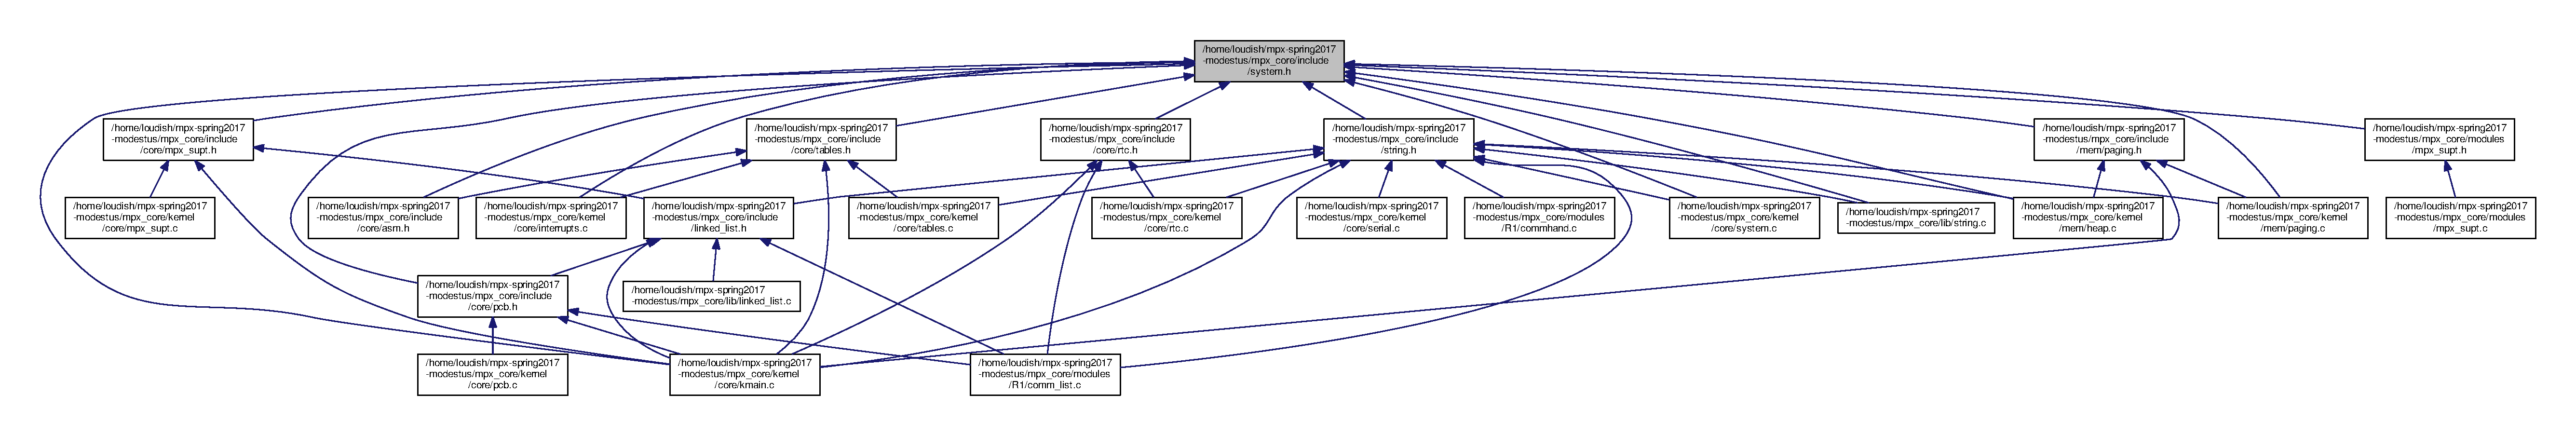
\includegraphics[width=350pt]{system_8h__dep__incl}
\end{center}
\end{figure}
\subsection*{Data Structures}
\begin{DoxyCompactItemize}
\item 
struct \hyperlink{structdate__time}{date\+\_\+time}
\end{DoxyCompactItemize}
\subsection*{Macros}
\begin{DoxyCompactItemize}
\item 
\#define \hyperlink{system_8h_a070d2ce7b6bb7e5c05602aa8c308d0c4}{N\+U\+LL}~0
\item 
\#define \hyperlink{system_8h_ab3bb695e7817363c7bdb781f214e83a2}{no\+\_\+warn}(p)~if (p) while (1) break
\item 
\#define \hyperlink{system_8h_a71921cebf4610b0dbb2b7a0daaf3fedf}{asm}~\+\_\+\+\_\+asm\+\_\+\+\_\+
\item 
\#define \hyperlink{system_8h_af55a5e48555be7d32ad73e76cf5d4db0}{volatile}~\+\_\+\+\_\+volatile\+\_\+\+\_\+
\item 
\#define \hyperlink{system_8h_ac5d15f274bc9b1e96230f3d3c60fd1f8}{sti}()~\hyperlink{system_8h_a71921cebf4610b0dbb2b7a0daaf3fedf}{asm} \hyperlink{system_8h_af55a5e48555be7d32ad73e76cf5d4db0}{volatile} (\char`\"{}sti\char`\"{}\+::)
\item 
\#define \hyperlink{system_8h_a68c330e94fe121eba993e5a5973c3162}{cli}()~\hyperlink{system_8h_a71921cebf4610b0dbb2b7a0daaf3fedf}{asm} \hyperlink{system_8h_af55a5e48555be7d32ad73e76cf5d4db0}{volatile} (\char`\"{}cli\char`\"{}\+::)
\item 
\#define \hyperlink{system_8h_a6c92c29fa8e83ab85e05543010e10d7c}{nop}()~\hyperlink{system_8h_a71921cebf4610b0dbb2b7a0daaf3fedf}{asm} \hyperlink{system_8h_af55a5e48555be7d32ad73e76cf5d4db0}{volatile} (\char`\"{}nop\char`\"{}\+::)
\item 
\#define \hyperlink{system_8h_a954b0134ce21d80f0efb22c77e821da3}{hlt}()~\hyperlink{system_8h_a71921cebf4610b0dbb2b7a0daaf3fedf}{asm} \hyperlink{system_8h_af55a5e48555be7d32ad73e76cf5d4db0}{volatile} (\char`\"{}hlt\char`\"{}\+::)
\item 
\#define \hyperlink{system_8h_a6eab829c77f5e1d2786863e18547b81b}{iret}()~\hyperlink{system_8h_a71921cebf4610b0dbb2b7a0daaf3fedf}{asm} \hyperlink{system_8h_af55a5e48555be7d32ad73e76cf5d4db0}{volatile} (\char`\"{}iret\char`\"{}\+::)
\item 
\#define \hyperlink{system_8h_aeb3dcf3cb65fb9b31c3d6b9ddb576071}{G\+D\+T\+\_\+\+C\+S\+\_\+\+ID}~0x01
\item 
\#define \hyperlink{system_8h_a90303dd4b4639f2e4106ced8d18fb4a1}{G\+D\+T\+\_\+\+D\+S\+\_\+\+ID}~0x02
\end{DoxyCompactItemize}
\subsection*{Typedefs}
\begin{DoxyCompactItemize}
\item 
typedef unsigned int \hyperlink{system_8h_a7c94ea6f8948649f8d181ae55911eeaf}{size\+\_\+t}
\item 
typedef unsigned char \hyperlink{system_8h_a1026e682ffdadc1701c42cd44ce9efcf}{u8int}
\item 
typedef unsigned short \hyperlink{system_8h_a863d9497073aad2b991aeab2211d87af}{u16int}
\item 
typedef unsigned long \hyperlink{system_8h_a757de76cafbcddaac0d1632902fe4cb8}{u32int}
\item 
typedef unsigned char \hyperlink{system_8h_aba7bc1797add20fe3efdf37ced1182c5}{uint8\+\_\+t}
\item 
typedef unsigned short \hyperlink{system_8h_a273cf69d639a59973b6019625df33e30}{uint16\+\_\+t}
\item 
typedef unsigned long \hyperlink{system_8h_a06896e8c53f721507066c079052171f8}{uint32\+\_\+t}
\end{DoxyCompactItemize}
\subsection*{Functions}
\begin{DoxyCompactItemize}
\item 
void \hyperlink{system_8h_abdb09834267dd4a2a0d07d43ca4d230d}{klogv} (const char $\ast$msg)
\item 
void \hyperlink{system_8h_aff8473f901d828d76d3548130731c41d}{kpanic} (const char $\ast$msg)
\end{DoxyCompactItemize}


\subsection{Macro Definition Documentation}
\index{system.\+h@{system.\+h}!asm@{asm}}
\index{asm@{asm}!system.\+h@{system.\+h}}
\subsubsection[{\texorpdfstring{asm}{asm}}]{\setlength{\rightskip}{0pt plus 5cm}\#define asm~\+\_\+\+\_\+asm\+\_\+\+\_\+}\hypertarget{system_8h_a71921cebf4610b0dbb2b7a0daaf3fedf}{}\label{system_8h_a71921cebf4610b0dbb2b7a0daaf3fedf}


Definition at line 11 of file system.\+h.

\index{system.\+h@{system.\+h}!cli@{cli}}
\index{cli@{cli}!system.\+h@{system.\+h}}
\subsubsection[{\texorpdfstring{cli}{cli}}]{\setlength{\rightskip}{0pt plus 5cm}\#define cli(
\begin{DoxyParamCaption}
{}
\end{DoxyParamCaption}
)~{\bf asm} {\bf volatile} (\char`\"{}cli\char`\"{}\+::)}\hypertarget{system_8h_a68c330e94fe121eba993e5a5973c3162}{}\label{system_8h_a68c330e94fe121eba993e5a5973c3162}


Definition at line 15 of file system.\+h.



Referenced by kmain(), kpanic(), set\+\_\+date(), and set\+\_\+time().

\index{system.\+h@{system.\+h}!G\+D\+T\+\_\+\+C\+S\+\_\+\+ID@{G\+D\+T\+\_\+\+C\+S\+\_\+\+ID}}
\index{G\+D\+T\+\_\+\+C\+S\+\_\+\+ID@{G\+D\+T\+\_\+\+C\+S\+\_\+\+ID}!system.\+h@{system.\+h}}
\subsubsection[{\texorpdfstring{G\+D\+T\+\_\+\+C\+S\+\_\+\+ID}{GDT_CS_ID}}]{\setlength{\rightskip}{0pt plus 5cm}\#define G\+D\+T\+\_\+\+C\+S\+\_\+\+ID~0x01}\hypertarget{system_8h_aeb3dcf3cb65fb9b31c3d6b9ddb576071}{}\label{system_8h_aeb3dcf3cb65fb9b31c3d6b9ddb576071}


Definition at line 20 of file system.\+h.

\index{system.\+h@{system.\+h}!G\+D\+T\+\_\+\+D\+S\+\_\+\+ID@{G\+D\+T\+\_\+\+D\+S\+\_\+\+ID}}
\index{G\+D\+T\+\_\+\+D\+S\+\_\+\+ID@{G\+D\+T\+\_\+\+D\+S\+\_\+\+ID}!system.\+h@{system.\+h}}
\subsubsection[{\texorpdfstring{G\+D\+T\+\_\+\+D\+S\+\_\+\+ID}{GDT_DS_ID}}]{\setlength{\rightskip}{0pt plus 5cm}\#define G\+D\+T\+\_\+\+D\+S\+\_\+\+ID~0x02}\hypertarget{system_8h_a90303dd4b4639f2e4106ced8d18fb4a1}{}\label{system_8h_a90303dd4b4639f2e4106ced8d18fb4a1}


Definition at line 21 of file system.\+h.

\index{system.\+h@{system.\+h}!hlt@{hlt}}
\index{hlt@{hlt}!system.\+h@{system.\+h}}
\subsubsection[{\texorpdfstring{hlt}{hlt}}]{\setlength{\rightskip}{0pt plus 5cm}\#define hlt(
\begin{DoxyParamCaption}
{}
\end{DoxyParamCaption}
)~{\bf asm} {\bf volatile} (\char`\"{}hlt\char`\"{}\+::)}\hypertarget{system_8h_a954b0134ce21d80f0efb22c77e821da3}{}\label{system_8h_a954b0134ce21d80f0efb22c77e821da3}


Definition at line 17 of file system.\+h.



Referenced by kmain(), and kpanic().

\index{system.\+h@{system.\+h}!iret@{iret}}
\index{iret@{iret}!system.\+h@{system.\+h}}
\subsubsection[{\texorpdfstring{iret}{iret}}]{\setlength{\rightskip}{0pt plus 5cm}\#define iret(
\begin{DoxyParamCaption}
{}
\end{DoxyParamCaption}
)~{\bf asm} {\bf volatile} (\char`\"{}iret\char`\"{}\+::)}\hypertarget{system_8h_a6eab829c77f5e1d2786863e18547b81b}{}\label{system_8h_a6eab829c77f5e1d2786863e18547b81b}


Definition at line 18 of file system.\+h.

\index{system.\+h@{system.\+h}!no\+\_\+warn@{no\+\_\+warn}}
\index{no\+\_\+warn@{no\+\_\+warn}!system.\+h@{system.\+h}}
\subsubsection[{\texorpdfstring{no\+\_\+warn}{no_warn}}]{\setlength{\rightskip}{0pt plus 5cm}\#define no\+\_\+warn(
\begin{DoxyParamCaption}
\item[{}]{p}
\end{DoxyParamCaption}
)~if (p) while (1) break}\hypertarget{system_8h_ab3bb695e7817363c7bdb781f214e83a2}{}\label{system_8h_ab3bb695e7817363c7bdb781f214e83a2}


Definition at line 7 of file system.\+h.



Referenced by alloc(), and make\+\_\+heap().

\index{system.\+h@{system.\+h}!nop@{nop}}
\index{nop@{nop}!system.\+h@{system.\+h}}
\subsubsection[{\texorpdfstring{nop}{nop}}]{\setlength{\rightskip}{0pt plus 5cm}\#define nop(
\begin{DoxyParamCaption}
{}
\end{DoxyParamCaption}
)~{\bf asm} {\bf volatile} (\char`\"{}nop\char`\"{}\+::)}\hypertarget{system_8h_a6c92c29fa8e83ab85e05543010e10d7c}{}\label{system_8h_a6c92c29fa8e83ab85e05543010e10d7c}


Definition at line 16 of file system.\+h.

\index{system.\+h@{system.\+h}!N\+U\+LL@{N\+U\+LL}}
\index{N\+U\+LL@{N\+U\+LL}!system.\+h@{system.\+h}}
\subsubsection[{\texorpdfstring{N\+U\+LL}{NULL}}]{\setlength{\rightskip}{0pt plus 5cm}\#define N\+U\+LL~0}\hypertarget{system_8h_a070d2ce7b6bb7e5c05602aa8c308d0c4}{}\label{system_8h_a070d2ce7b6bb7e5c05602aa8c308d0c4}


Definition at line 4 of file system.\+h.



Referenced by parse\+\_\+comm(), and strtok().

\index{system.\+h@{system.\+h}!sti@{sti}}
\index{sti@{sti}!system.\+h@{system.\+h}}
\subsubsection[{\texorpdfstring{sti}{sti}}]{\setlength{\rightskip}{0pt plus 5cm}\#define sti(
\begin{DoxyParamCaption}
{}
\end{DoxyParamCaption}
)~{\bf asm} {\bf volatile} (\char`\"{}sti\char`\"{}\+::)}\hypertarget{system_8h_ac5d15f274bc9b1e96230f3d3c60fd1f8}{}\label{system_8h_ac5d15f274bc9b1e96230f3d3c60fd1f8}


Definition at line 14 of file system.\+h.



Referenced by set\+\_\+date(), and set\+\_\+time().

\index{system.\+h@{system.\+h}!volatile@{volatile}}
\index{volatile@{volatile}!system.\+h@{system.\+h}}
\subsubsection[{\texorpdfstring{volatile}{volatile}}]{\setlength{\rightskip}{0pt plus 5cm}\#define volatile~\+\_\+\+\_\+volatile\+\_\+\+\_\+}\hypertarget{system_8h_af55a5e48555be7d32ad73e76cf5d4db0}{}\label{system_8h_af55a5e48555be7d32ad73e76cf5d4db0}


Definition at line 12 of file system.\+h.



\subsection{Typedef Documentation}
\index{system.\+h@{system.\+h}!size\+\_\+t@{size\+\_\+t}}
\index{size\+\_\+t@{size\+\_\+t}!system.\+h@{system.\+h}}
\subsubsection[{\texorpdfstring{size\+\_\+t}{size_t}}]{\setlength{\rightskip}{0pt plus 5cm}typedef unsigned int {\bf size\+\_\+t}}\hypertarget{system_8h_a7c94ea6f8948649f8d181ae55911eeaf}{}\label{system_8h_a7c94ea6f8948649f8d181ae55911eeaf}


Definition at line 24 of file system.\+h.

\index{system.\+h@{system.\+h}!u16int@{u16int}}
\index{u16int@{u16int}!system.\+h@{system.\+h}}
\subsubsection[{\texorpdfstring{u16int}{u16int}}]{\setlength{\rightskip}{0pt plus 5cm}typedef unsigned short {\bf u16int}}\hypertarget{system_8h_a863d9497073aad2b991aeab2211d87af}{}\label{system_8h_a863d9497073aad2b991aeab2211d87af}


Definition at line 26 of file system.\+h.

\index{system.\+h@{system.\+h}!u32int@{u32int}}
\index{u32int@{u32int}!system.\+h@{system.\+h}}
\subsubsection[{\texorpdfstring{u32int}{u32int}}]{\setlength{\rightskip}{0pt plus 5cm}typedef unsigned long {\bf u32int}}\hypertarget{system_8h_a757de76cafbcddaac0d1632902fe4cb8}{}\label{system_8h_a757de76cafbcddaac0d1632902fe4cb8}


Definition at line 27 of file system.\+h.

\index{system.\+h@{system.\+h}!u8int@{u8int}}
\index{u8int@{u8int}!system.\+h@{system.\+h}}
\subsubsection[{\texorpdfstring{u8int}{u8int}}]{\setlength{\rightskip}{0pt plus 5cm}typedef unsigned char {\bf u8int}}\hypertarget{system_8h_a1026e682ffdadc1701c42cd44ce9efcf}{}\label{system_8h_a1026e682ffdadc1701c42cd44ce9efcf}


Definition at line 25 of file system.\+h.

\index{system.\+h@{system.\+h}!uint16\+\_\+t@{uint16\+\_\+t}}
\index{uint16\+\_\+t@{uint16\+\_\+t}!system.\+h@{system.\+h}}
\subsubsection[{\texorpdfstring{uint16\+\_\+t}{uint16_t}}]{\setlength{\rightskip}{0pt plus 5cm}typedef unsigned short {\bf uint16\+\_\+t}}\hypertarget{system_8h_a273cf69d639a59973b6019625df33e30}{}\label{system_8h_a273cf69d639a59973b6019625df33e30}


Definition at line 30 of file system.\+h.

\index{system.\+h@{system.\+h}!uint32\+\_\+t@{uint32\+\_\+t}}
\index{uint32\+\_\+t@{uint32\+\_\+t}!system.\+h@{system.\+h}}
\subsubsection[{\texorpdfstring{uint32\+\_\+t}{uint32_t}}]{\setlength{\rightskip}{0pt plus 5cm}typedef unsigned long {\bf uint32\+\_\+t}}\hypertarget{system_8h_a06896e8c53f721507066c079052171f8}{}\label{system_8h_a06896e8c53f721507066c079052171f8}


Definition at line 31 of file system.\+h.

\index{system.\+h@{system.\+h}!uint8\+\_\+t@{uint8\+\_\+t}}
\index{uint8\+\_\+t@{uint8\+\_\+t}!system.\+h@{system.\+h}}
\subsubsection[{\texorpdfstring{uint8\+\_\+t}{uint8_t}}]{\setlength{\rightskip}{0pt plus 5cm}typedef unsigned char {\bf uint8\+\_\+t}}\hypertarget{system_8h_aba7bc1797add20fe3efdf37ced1182c5}{}\label{system_8h_aba7bc1797add20fe3efdf37ced1182c5}


Definition at line 29 of file system.\+h.



\subsection{Function Documentation}
\index{system.\+h@{system.\+h}!klogv@{klogv}}
\index{klogv@{klogv}!system.\+h@{system.\+h}}
\subsubsection[{\texorpdfstring{klogv(const char $\ast$msg)}{klogv(const char *msg)}}]{\setlength{\rightskip}{0pt plus 5cm}void klogv (
\begin{DoxyParamCaption}
\item[{const char $\ast$}]{msg}
\end{DoxyParamCaption}
)}\hypertarget{system_8h_abdb09834267dd4a2a0d07d43ca4d230d}{}\label{system_8h_abdb09834267dd4a2a0d07d43ca4d230d}


Definition at line 11 of file system.\+c.



References serial\+\_\+println(), and strcat().



Referenced by kmain(), and kpanic().


\begin{DoxyCode}
12 \{
13   \textcolor{keywordtype}{char} logmsg[64] = \{\textcolor{charliteral}{'\(\backslash\)0'}\}, prefix[] = \textcolor{stringliteral}{"klogv: "};
14   \hyperlink{string_8h_a8908188ae9fc2f05d993257ef001d553}{strcat}(logmsg, prefix);
15   \hyperlink{string_8h_a8908188ae9fc2f05d993257ef001d553}{strcat}(logmsg, msg);
16   \hyperlink{serial_8h_a3514f7abff236a4e00a6c46021ce5e22}{serial\_println}(logmsg);
17 \}
\end{DoxyCode}
\index{system.\+h@{system.\+h}!kpanic@{kpanic}}
\index{kpanic@{kpanic}!system.\+h@{system.\+h}}
\subsubsection[{\texorpdfstring{kpanic(const char $\ast$msg)}{kpanic(const char *msg)}}]{\setlength{\rightskip}{0pt plus 5cm}void kpanic (
\begin{DoxyParamCaption}
\item[{const char $\ast$}]{msg}
\end{DoxyParamCaption}
)}\hypertarget{system_8h_aff8473f901d828d76d3548130731c41d}{}\label{system_8h_aff8473f901d828d76d3548130731c41d}


Definition at line 24 of file system.\+c.



References cli, hlt, klogv(), and strcat().



Referenced by do\+\_\+bounds(), do\+\_\+breakpoint(), do\+\_\+coprocessor(), do\+\_\+coprocessor\+\_\+segment(), do\+\_\+debug(), do\+\_\+device\+\_\+not\+\_\+available(), do\+\_\+divide\+\_\+error(), do\+\_\+double\+\_\+fault(), do\+\_\+general\+\_\+protection(), do\+\_\+invalid\+\_\+op(), do\+\_\+invalid\+\_\+tss(), do\+\_\+nmi(), do\+\_\+overflow(), do\+\_\+page\+\_\+fault(), do\+\_\+segment\+\_\+not\+\_\+present(), do\+\_\+stack\+\_\+segment(), and new\+\_\+frame().


\begin{DoxyCode}
25 \{
26   \hyperlink{system_8h_a68c330e94fe121eba993e5a5973c3162}{cli}(); \textcolor{comment}{//disable interrupts}
27   \textcolor{keywordtype}{char} logmsg[64] = \{\textcolor{charliteral}{'\(\backslash\)0'}\}, prefix[] = \textcolor{stringliteral}{"Panic: "};
28   \hyperlink{string_8h_a8908188ae9fc2f05d993257ef001d553}{strcat}(logmsg, prefix);
29   \hyperlink{string_8h_a8908188ae9fc2f05d993257ef001d553}{strcat}(logmsg, msg);
30   \hyperlink{system_8c_abdb09834267dd4a2a0d07d43ca4d230d}{klogv}(logmsg);
31   \hyperlink{system_8h_a954b0134ce21d80f0efb22c77e821da3}{hlt}(); \textcolor{comment}{//halt}
32 \}
\end{DoxyCode}

\hypertarget{interrupts_8c}{}\section{/home/loudish/mpx-\/spring2017-\/modestus/mpx\+\_\+core/kernel/core/interrupts.c File Reference}
\label{interrupts_8c}\index{/home/loudish/mpx-\/spring2017-\/modestus/mpx\+\_\+core/kernel/core/interrupts.\+c@{/home/loudish/mpx-\/spring2017-\/modestus/mpx\+\_\+core/kernel/core/interrupts.\+c}}
{\ttfamily \#include $<$system.\+h$>$}\\*
{\ttfamily \#include $<$core/io.\+h$>$}\\*
{\ttfamily \#include $<$core/serial.\+h$>$}\\*
{\ttfamily \#include $<$core/tables.\+h$>$}\\*
{\ttfamily \#include $<$core/interrupts.\+h$>$}\\*
Include dependency graph for interrupts.\+c\+:\nopagebreak
\begin{figure}[H]
\begin{center}
\leavevmode
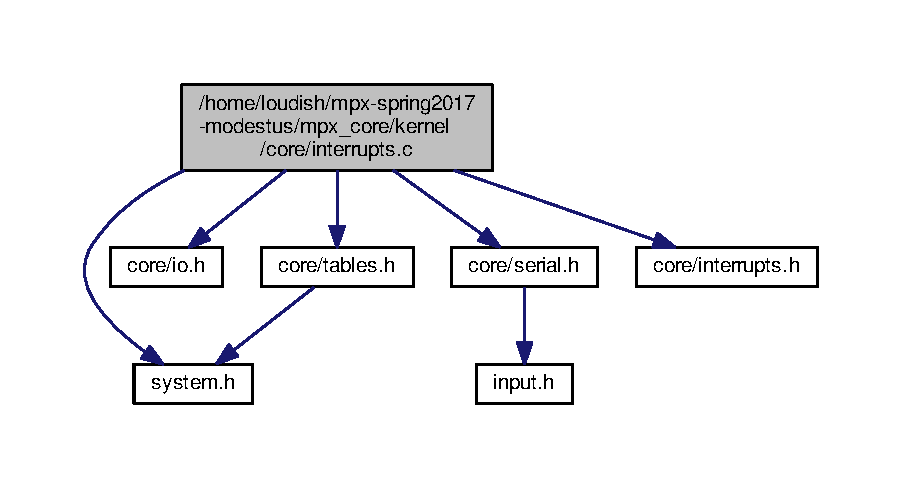
\includegraphics[width=350pt]{interrupts_8c__incl}
\end{center}
\end{figure}
\subsection*{Macros}
\begin{DoxyCompactItemize}
\item 
\#define \hyperlink{interrupts_8c_a6b115109e4a0d3c5fb6252d091e86bfe}{P\+I\+C1}~0x20
\item 
\#define \hyperlink{interrupts_8c_ac90003f52c8d736193efc954ece08e58}{P\+I\+C2}~0x\+A0
\item 
\#define \hyperlink{interrupts_8c_ac56445256ce58f14f3c61af0cbf0cdad}{I\+C\+W1}~0x11
\item 
\#define \hyperlink{interrupts_8c_a7945f331ddf94a0e0e938f825bc4d43c}{I\+C\+W4}~0x01
\item 
\#define \hyperlink{interrupts_8c_aeae4190ed25d0648577e1c742fd8a78d}{io\+\_\+wait}()~\hyperlink{system_8h_a71921cebf4610b0dbb2b7a0daaf3fedf}{asm} \hyperlink{system_8h_af55a5e48555be7d32ad73e76cf5d4db0}{volatile} (\char`\"{}outb \$0x80\char`\"{})
\end{DoxyCompactItemize}
\subsection*{Functions}
\begin{DoxyCompactItemize}
\item 
void \hyperlink{interrupts_8c_a779cbe32e1a5f1dc8fa9b7191f116b28}{divide\+\_\+error} ()
\item 
void \hyperlink{interrupts_8c_a0d0105433f9c65c14928027b3f0966b7}{debug} ()
\item 
void \hyperlink{interrupts_8c_aa42d18df06cf68f8c05fded5344c4c7e}{nmi} ()
\item 
void \hyperlink{interrupts_8c_a874043e2396dd8ce20ec7af3ea1e2a86}{breakpoint} ()
\item 
void \hyperlink{interrupts_8c_a810f078a27a6781a7406c74985ecb761}{overflow} ()
\item 
void \hyperlink{interrupts_8c_a96724d36ad85f9a02231d8e6fe0434df}{bounds} ()
\item 
void \hyperlink{interrupts_8c_a422d8af60b69cc11dbcbb9d89c69756b}{invalid\+\_\+op} ()
\item 
void \hyperlink{interrupts_8c_abe88cd1dcc26cb58ee785c714e016f72}{device\+\_\+not\+\_\+available} ()
\item 
void \hyperlink{interrupts_8c_ae2b9f5b44e05e0c53f8eaaa98396d627}{double\+\_\+fault} ()
\item 
void \hyperlink{interrupts_8c_a1d688a0a370977c03fa98884a6e771e9}{coprocessor\+\_\+segment} ()
\item 
void \hyperlink{interrupts_8c_a972be67f6a5432cc8eab8d27755fb00f}{invalid\+\_\+tss} ()
\item 
void \hyperlink{interrupts_8c_af1748d9ea65ba652bc92074ab6570d8e}{segment\+\_\+not\+\_\+present} ()
\item 
void \hyperlink{interrupts_8c_a1ccc3198890318741629a03bb88bee6f}{stack\+\_\+segment} ()
\item 
void \hyperlink{interrupts_8c_a10777dd6c3a040471676741bbb8dda46}{general\+\_\+protection} ()
\item 
void \hyperlink{interrupts_8c_ab3800dd0177baaef4da00494edfb32d9}{page\+\_\+fault} ()
\item 
void \hyperlink{interrupts_8c_ad686e3fee8ec8346a6d8e98d970a02dd}{reserved} ()
\item 
void \hyperlink{interrupts_8c_a5c538c7b7a55e3c981780b599fcb1de7}{coprocessor} ()
\item 
void \hyperlink{interrupts_8c_a52f2615cebbdeab188085a03c913fcf9}{rtc\+\_\+isr} ()
\item 
void \hyperlink{interrupts_8c_af88eb8e98d943aa0461c01de3cb53493}{isr0} ()
\item 
void \hyperlink{interrupts_8c_a1f9ba1353a3e7fcf94720c1c56ab3a96}{do\+\_\+isr} ()
\item 
void \hyperlink{interrupts_8c_ad17d9a8aa78440af8fc40d3fd55dbad8}{init\+\_\+irq} (void)
\item 
void \hyperlink{interrupts_8c_afbc0dbef6f15e2df21b38724ea38c483}{init\+\_\+pic} (void)
\item 
void \hyperlink{interrupts_8c_aab29cc64234c341b5d2efc6cc8f68714}{do\+\_\+divide\+\_\+error} ()
\item 
void \hyperlink{interrupts_8c_ac3cb74146ddcc548b98534fc275e6672}{do\+\_\+debug} ()
\item 
void \hyperlink{interrupts_8c_a32aec16299751a52f0a12f26043c0d7d}{do\+\_\+nmi} ()
\item 
void \hyperlink{interrupts_8c_a0ea01197b18487b9e94d20d83055d743}{do\+\_\+breakpoint} ()
\item 
void \hyperlink{interrupts_8c_a49e352bcfc8f4fadf35bd6a263bedebe}{do\+\_\+overflow} ()
\item 
void \hyperlink{interrupts_8c_a27f47460ebcce0c6a6af781bd6f9fb9f}{do\+\_\+bounds} ()
\item 
void \hyperlink{interrupts_8c_abed3b5d3250b216bc700d29085f5b0c9}{do\+\_\+invalid\+\_\+op} ()
\item 
void \hyperlink{interrupts_8c_a45efb1fd58094c1e71b1d2423f3971f6}{do\+\_\+device\+\_\+not\+\_\+available} ()
\item 
void \hyperlink{interrupts_8c_a1c92f7e610e78af13b2d9a2d962cc4e6}{do\+\_\+double\+\_\+fault} ()
\item 
void \hyperlink{interrupts_8c_af5be233a6560c8dcf2ac87eafbee7e0e}{do\+\_\+coprocessor\+\_\+segment} ()
\item 
void \hyperlink{interrupts_8c_a4470fee2d72940bf23ec1510c20582c3}{do\+\_\+invalid\+\_\+tss} ()
\item 
void \hyperlink{interrupts_8c_ac36f6e131887ab7f2e9e4f93858f8a34}{do\+\_\+segment\+\_\+not\+\_\+present} ()
\item 
void \hyperlink{interrupts_8c_a70282e61c45bf8c1b0ace8021977207d}{do\+\_\+stack\+\_\+segment} ()
\item 
void \hyperlink{interrupts_8c_a6b1e503d397160ae65963ef495a10dfd}{do\+\_\+general\+\_\+protection} ()
\item 
void \hyperlink{interrupts_8c_a70473c7f1d2679277751cb161e2d768d}{do\+\_\+page\+\_\+fault} ()
\item 
void \hyperlink{interrupts_8c_a3b448798302562f8ef16b8ee1de71ba7}{do\+\_\+reserved} ()
\item 
void \hyperlink{interrupts_8c_a8a3725c251a2cb8e346a847febf66ed2}{do\+\_\+coprocessor} ()
\end{DoxyCompactItemize}
\subsection*{Variables}
\begin{DoxyCompactItemize}
\item 
idt\+\_\+entry \hyperlink{interrupts_8c_a3c386c59636822ce451be20cc1433a55}{idt\+\_\+entries} \mbox{[}256\mbox{]}
\end{DoxyCompactItemize}


\subsection{Macro Definition Documentation}
\index{interrupts.\+c@{interrupts.\+c}!I\+C\+W1@{I\+C\+W1}}
\index{I\+C\+W1@{I\+C\+W1}!interrupts.\+c@{interrupts.\+c}}
\subsubsection[{\texorpdfstring{I\+C\+W1}{ICW1}}]{\setlength{\rightskip}{0pt plus 5cm}\#define I\+C\+W1~0x11}\hypertarget{interrupts_8c_ac56445256ce58f14f3c61af0cbf0cdad}{}\label{interrupts_8c_ac56445256ce58f14f3c61af0cbf0cdad}


Definition at line 20 of file interrupts.\+c.



Referenced by init\+\_\+pic().

\index{interrupts.\+c@{interrupts.\+c}!I\+C\+W4@{I\+C\+W4}}
\index{I\+C\+W4@{I\+C\+W4}!interrupts.\+c@{interrupts.\+c}}
\subsubsection[{\texorpdfstring{I\+C\+W4}{ICW4}}]{\setlength{\rightskip}{0pt plus 5cm}\#define I\+C\+W4~0x01}\hypertarget{interrupts_8c_a7945f331ddf94a0e0e938f825bc4d43c}{}\label{interrupts_8c_a7945f331ddf94a0e0e938f825bc4d43c}


Definition at line 21 of file interrupts.\+c.



Referenced by init\+\_\+pic().

\index{interrupts.\+c@{interrupts.\+c}!io\+\_\+wait@{io\+\_\+wait}}
\index{io\+\_\+wait@{io\+\_\+wait}!interrupts.\+c@{interrupts.\+c}}
\subsubsection[{\texorpdfstring{io\+\_\+wait}{io_wait}}]{\setlength{\rightskip}{0pt plus 5cm}\#define io\+\_\+wait(
\begin{DoxyParamCaption}
{}
\end{DoxyParamCaption}
)~{\bf asm} {\bf volatile} (\char`\"{}outb \$0x80\char`\"{})}\hypertarget{interrupts_8c_aeae4190ed25d0648577e1c742fd8a78d}{}\label{interrupts_8c_aeae4190ed25d0648577e1c742fd8a78d}


Definition at line 28 of file interrupts.\+c.



Referenced by init\+\_\+pic().

\index{interrupts.\+c@{interrupts.\+c}!P\+I\+C1@{P\+I\+C1}}
\index{P\+I\+C1@{P\+I\+C1}!interrupts.\+c@{interrupts.\+c}}
\subsubsection[{\texorpdfstring{P\+I\+C1}{PIC1}}]{\setlength{\rightskip}{0pt plus 5cm}\#define P\+I\+C1~0x20}\hypertarget{interrupts_8c_a6b115109e4a0d3c5fb6252d091e86bfe}{}\label{interrupts_8c_a6b115109e4a0d3c5fb6252d091e86bfe}


Definition at line 16 of file interrupts.\+c.



Referenced by init\+\_\+pic().

\index{interrupts.\+c@{interrupts.\+c}!P\+I\+C2@{P\+I\+C2}}
\index{P\+I\+C2@{P\+I\+C2}!interrupts.\+c@{interrupts.\+c}}
\subsubsection[{\texorpdfstring{P\+I\+C2}{PIC2}}]{\setlength{\rightskip}{0pt plus 5cm}\#define P\+I\+C2~0x\+A0}\hypertarget{interrupts_8c_ac90003f52c8d736193efc954ece08e58}{}\label{interrupts_8c_ac90003f52c8d736193efc954ece08e58}


Definition at line 17 of file interrupts.\+c.



Referenced by init\+\_\+pic().



\subsection{Function Documentation}
\index{interrupts.\+c@{interrupts.\+c}!bounds@{bounds}}
\index{bounds@{bounds}!interrupts.\+c@{interrupts.\+c}}
\subsubsection[{\texorpdfstring{bounds()}{bounds()}}]{\setlength{\rightskip}{0pt plus 5cm}void bounds (
\begin{DoxyParamCaption}
{}
\end{DoxyParamCaption}
)}\hypertarget{interrupts_8c_a96724d36ad85f9a02231d8e6fe0434df}{}\label{interrupts_8c_a96724d36ad85f9a02231d8e6fe0434df}


Referenced by init\+\_\+irq().

\index{interrupts.\+c@{interrupts.\+c}!breakpoint@{breakpoint}}
\index{breakpoint@{breakpoint}!interrupts.\+c@{interrupts.\+c}}
\subsubsection[{\texorpdfstring{breakpoint()}{breakpoint()}}]{\setlength{\rightskip}{0pt plus 5cm}void breakpoint (
\begin{DoxyParamCaption}
{}
\end{DoxyParamCaption}
)}\hypertarget{interrupts_8c_a874043e2396dd8ce20ec7af3ea1e2a86}{}\label{interrupts_8c_a874043e2396dd8ce20ec7af3ea1e2a86}


Referenced by init\+\_\+irq().

\index{interrupts.\+c@{interrupts.\+c}!coprocessor@{coprocessor}}
\index{coprocessor@{coprocessor}!interrupts.\+c@{interrupts.\+c}}
\subsubsection[{\texorpdfstring{coprocessor()}{coprocessor()}}]{\setlength{\rightskip}{0pt plus 5cm}void coprocessor (
\begin{DoxyParamCaption}
{}
\end{DoxyParamCaption}
)}\hypertarget{interrupts_8c_a5c538c7b7a55e3c981780b599fcb1de7}{}\label{interrupts_8c_a5c538c7b7a55e3c981780b599fcb1de7}


Referenced by init\+\_\+irq().

\index{interrupts.\+c@{interrupts.\+c}!coprocessor\+\_\+segment@{coprocessor\+\_\+segment}}
\index{coprocessor\+\_\+segment@{coprocessor\+\_\+segment}!interrupts.\+c@{interrupts.\+c}}
\subsubsection[{\texorpdfstring{coprocessor\+\_\+segment()}{coprocessor_segment()}}]{\setlength{\rightskip}{0pt plus 5cm}void coprocessor\+\_\+segment (
\begin{DoxyParamCaption}
{}
\end{DoxyParamCaption}
)}\hypertarget{interrupts_8c_a1d688a0a370977c03fa98884a6e771e9}{}\label{interrupts_8c_a1d688a0a370977c03fa98884a6e771e9}


Referenced by init\+\_\+irq().

\index{interrupts.\+c@{interrupts.\+c}!debug@{debug}}
\index{debug@{debug}!interrupts.\+c@{interrupts.\+c}}
\subsubsection[{\texorpdfstring{debug()}{debug()}}]{\setlength{\rightskip}{0pt plus 5cm}void debug (
\begin{DoxyParamCaption}
{}
\end{DoxyParamCaption}
)}\hypertarget{interrupts_8c_a0d0105433f9c65c14928027b3f0966b7}{}\label{interrupts_8c_a0d0105433f9c65c14928027b3f0966b7}


Referenced by init\+\_\+irq().

\index{interrupts.\+c@{interrupts.\+c}!device\+\_\+not\+\_\+available@{device\+\_\+not\+\_\+available}}
\index{device\+\_\+not\+\_\+available@{device\+\_\+not\+\_\+available}!interrupts.\+c@{interrupts.\+c}}
\subsubsection[{\texorpdfstring{device\+\_\+not\+\_\+available()}{device_not_available()}}]{\setlength{\rightskip}{0pt plus 5cm}void device\+\_\+not\+\_\+available (
\begin{DoxyParamCaption}
{}
\end{DoxyParamCaption}
)}\hypertarget{interrupts_8c_abe88cd1dcc26cb58ee785c714e016f72}{}\label{interrupts_8c_abe88cd1dcc26cb58ee785c714e016f72}


Referenced by init\+\_\+irq().

\index{interrupts.\+c@{interrupts.\+c}!divide\+\_\+error@{divide\+\_\+error}}
\index{divide\+\_\+error@{divide\+\_\+error}!interrupts.\+c@{interrupts.\+c}}
\subsubsection[{\texorpdfstring{divide\+\_\+error()}{divide_error()}}]{\setlength{\rightskip}{0pt plus 5cm}void divide\+\_\+error (
\begin{DoxyParamCaption}
{}
\end{DoxyParamCaption}
)}\hypertarget{interrupts_8c_a779cbe32e1a5f1dc8fa9b7191f116b28}{}\label{interrupts_8c_a779cbe32e1a5f1dc8fa9b7191f116b28}


Referenced by init\+\_\+irq().

\index{interrupts.\+c@{interrupts.\+c}!do\+\_\+bounds@{do\+\_\+bounds}}
\index{do\+\_\+bounds@{do\+\_\+bounds}!interrupts.\+c@{interrupts.\+c}}
\subsubsection[{\texorpdfstring{do\+\_\+bounds()}{do_bounds()}}]{\setlength{\rightskip}{0pt plus 5cm}void do\+\_\+bounds (
\begin{DoxyParamCaption}
{}
\end{DoxyParamCaption}
)}\hypertarget{interrupts_8c_a27f47460ebcce0c6a6af781bd6f9fb9f}{}\label{interrupts_8c_a27f47460ebcce0c6a6af781bd6f9fb9f}


Definition at line 149 of file interrupts.\+c.



References kpanic().


\begin{DoxyCode}
150 \{
151   \hyperlink{system_8h_aff8473f901d828d76d3548130731c41d}{kpanic}(\textcolor{stringliteral}{"Bounds error"});
152 \}
\end{DoxyCode}
\index{interrupts.\+c@{interrupts.\+c}!do\+\_\+breakpoint@{do\+\_\+breakpoint}}
\index{do\+\_\+breakpoint@{do\+\_\+breakpoint}!interrupts.\+c@{interrupts.\+c}}
\subsubsection[{\texorpdfstring{do\+\_\+breakpoint()}{do_breakpoint()}}]{\setlength{\rightskip}{0pt plus 5cm}void do\+\_\+breakpoint (
\begin{DoxyParamCaption}
{}
\end{DoxyParamCaption}
)}\hypertarget{interrupts_8c_a0ea01197b18487b9e94d20d83055d743}{}\label{interrupts_8c_a0ea01197b18487b9e94d20d83055d743}


Definition at line 141 of file interrupts.\+c.



References kpanic().


\begin{DoxyCode}
142 \{
143   \hyperlink{system_8h_aff8473f901d828d76d3548130731c41d}{kpanic}(\textcolor{stringliteral}{"Breakpoint"});
144 \}
\end{DoxyCode}
\index{interrupts.\+c@{interrupts.\+c}!do\+\_\+coprocessor@{do\+\_\+coprocessor}}
\index{do\+\_\+coprocessor@{do\+\_\+coprocessor}!interrupts.\+c@{interrupts.\+c}}
\subsubsection[{\texorpdfstring{do\+\_\+coprocessor()}{do_coprocessor()}}]{\setlength{\rightskip}{0pt plus 5cm}void do\+\_\+coprocessor (
\begin{DoxyParamCaption}
{}
\end{DoxyParamCaption}
)}\hypertarget{interrupts_8c_a8a3725c251a2cb8e346a847febf66ed2}{}\label{interrupts_8c_a8a3725c251a2cb8e346a847febf66ed2}


Definition at line 193 of file interrupts.\+c.



References kpanic().


\begin{DoxyCode}
194 \{
195   \hyperlink{system_8h_aff8473f901d828d76d3548130731c41d}{kpanic}(\textcolor{stringliteral}{"Coprocessor error"});
196 \}
\end{DoxyCode}
\index{interrupts.\+c@{interrupts.\+c}!do\+\_\+coprocessor\+\_\+segment@{do\+\_\+coprocessor\+\_\+segment}}
\index{do\+\_\+coprocessor\+\_\+segment@{do\+\_\+coprocessor\+\_\+segment}!interrupts.\+c@{interrupts.\+c}}
\subsubsection[{\texorpdfstring{do\+\_\+coprocessor\+\_\+segment()}{do_coprocessor_segment()}}]{\setlength{\rightskip}{0pt plus 5cm}void do\+\_\+coprocessor\+\_\+segment (
\begin{DoxyParamCaption}
{}
\end{DoxyParamCaption}
)}\hypertarget{interrupts_8c_af5be233a6560c8dcf2ac87eafbee7e0e}{}\label{interrupts_8c_af5be233a6560c8dcf2ac87eafbee7e0e}


Definition at line 165 of file interrupts.\+c.



References kpanic().


\begin{DoxyCode}
166 \{
167   \hyperlink{system_8h_aff8473f901d828d76d3548130731c41d}{kpanic}(\textcolor{stringliteral}{"Coprocessor segment error"});
168 \}
\end{DoxyCode}
\index{interrupts.\+c@{interrupts.\+c}!do\+\_\+debug@{do\+\_\+debug}}
\index{do\+\_\+debug@{do\+\_\+debug}!interrupts.\+c@{interrupts.\+c}}
\subsubsection[{\texorpdfstring{do\+\_\+debug()}{do_debug()}}]{\setlength{\rightskip}{0pt plus 5cm}void do\+\_\+debug (
\begin{DoxyParamCaption}
{}
\end{DoxyParamCaption}
)}\hypertarget{interrupts_8c_ac3cb74146ddcc548b98534fc275e6672}{}\label{interrupts_8c_ac3cb74146ddcc548b98534fc275e6672}


Definition at line 133 of file interrupts.\+c.



References kpanic().


\begin{DoxyCode}
134 \{
135   \hyperlink{system_8h_aff8473f901d828d76d3548130731c41d}{kpanic}(\textcolor{stringliteral}{"Debug"});
136 \}
\end{DoxyCode}
\index{interrupts.\+c@{interrupts.\+c}!do\+\_\+device\+\_\+not\+\_\+available@{do\+\_\+device\+\_\+not\+\_\+available}}
\index{do\+\_\+device\+\_\+not\+\_\+available@{do\+\_\+device\+\_\+not\+\_\+available}!interrupts.\+c@{interrupts.\+c}}
\subsubsection[{\texorpdfstring{do\+\_\+device\+\_\+not\+\_\+available()}{do_device_not_available()}}]{\setlength{\rightskip}{0pt plus 5cm}void do\+\_\+device\+\_\+not\+\_\+available (
\begin{DoxyParamCaption}
{}
\end{DoxyParamCaption}
)}\hypertarget{interrupts_8c_a45efb1fd58094c1e71b1d2423f3971f6}{}\label{interrupts_8c_a45efb1fd58094c1e71b1d2423f3971f6}


Definition at line 157 of file interrupts.\+c.



References kpanic().


\begin{DoxyCode}
158 \{
159   \hyperlink{system_8h_aff8473f901d828d76d3548130731c41d}{kpanic}(\textcolor{stringliteral}{"Device not available"});
160 \}
\end{DoxyCode}
\index{interrupts.\+c@{interrupts.\+c}!do\+\_\+divide\+\_\+error@{do\+\_\+divide\+\_\+error}}
\index{do\+\_\+divide\+\_\+error@{do\+\_\+divide\+\_\+error}!interrupts.\+c@{interrupts.\+c}}
\subsubsection[{\texorpdfstring{do\+\_\+divide\+\_\+error()}{do_divide_error()}}]{\setlength{\rightskip}{0pt plus 5cm}void do\+\_\+divide\+\_\+error (
\begin{DoxyParamCaption}
{}
\end{DoxyParamCaption}
)}\hypertarget{interrupts_8c_aab29cc64234c341b5d2efc6cc8f68714}{}\label{interrupts_8c_aab29cc64234c341b5d2efc6cc8f68714}


Definition at line 129 of file interrupts.\+c.



References kpanic().


\begin{DoxyCode}
130 \{
131   \hyperlink{system_8h_aff8473f901d828d76d3548130731c41d}{kpanic}(\textcolor{stringliteral}{"Division-by-zero"});
132 \}
\end{DoxyCode}
\index{interrupts.\+c@{interrupts.\+c}!do\+\_\+double\+\_\+fault@{do\+\_\+double\+\_\+fault}}
\index{do\+\_\+double\+\_\+fault@{do\+\_\+double\+\_\+fault}!interrupts.\+c@{interrupts.\+c}}
\subsubsection[{\texorpdfstring{do\+\_\+double\+\_\+fault()}{do_double_fault()}}]{\setlength{\rightskip}{0pt plus 5cm}void do\+\_\+double\+\_\+fault (
\begin{DoxyParamCaption}
{}
\end{DoxyParamCaption}
)}\hypertarget{interrupts_8c_a1c92f7e610e78af13b2d9a2d962cc4e6}{}\label{interrupts_8c_a1c92f7e610e78af13b2d9a2d962cc4e6}


Definition at line 161 of file interrupts.\+c.



References kpanic().


\begin{DoxyCode}
162 \{
163   \hyperlink{system_8h_aff8473f901d828d76d3548130731c41d}{kpanic}(\textcolor{stringliteral}{"Double fault"});
164 \}
\end{DoxyCode}
\index{interrupts.\+c@{interrupts.\+c}!do\+\_\+general\+\_\+protection@{do\+\_\+general\+\_\+protection}}
\index{do\+\_\+general\+\_\+protection@{do\+\_\+general\+\_\+protection}!interrupts.\+c@{interrupts.\+c}}
\subsubsection[{\texorpdfstring{do\+\_\+general\+\_\+protection()}{do_general_protection()}}]{\setlength{\rightskip}{0pt plus 5cm}void do\+\_\+general\+\_\+protection (
\begin{DoxyParamCaption}
{}
\end{DoxyParamCaption}
)}\hypertarget{interrupts_8c_a6b1e503d397160ae65963ef495a10dfd}{}\label{interrupts_8c_a6b1e503d397160ae65963ef495a10dfd}


Definition at line 181 of file interrupts.\+c.



References kpanic().


\begin{DoxyCode}
182 \{
183   \hyperlink{system_8h_aff8473f901d828d76d3548130731c41d}{kpanic}(\textcolor{stringliteral}{"General protection fault"});
184 \}
\end{DoxyCode}
\index{interrupts.\+c@{interrupts.\+c}!do\+\_\+invalid\+\_\+op@{do\+\_\+invalid\+\_\+op}}
\index{do\+\_\+invalid\+\_\+op@{do\+\_\+invalid\+\_\+op}!interrupts.\+c@{interrupts.\+c}}
\subsubsection[{\texorpdfstring{do\+\_\+invalid\+\_\+op()}{do_invalid_op()}}]{\setlength{\rightskip}{0pt plus 5cm}void do\+\_\+invalid\+\_\+op (
\begin{DoxyParamCaption}
{}
\end{DoxyParamCaption}
)}\hypertarget{interrupts_8c_abed3b5d3250b216bc700d29085f5b0c9}{}\label{interrupts_8c_abed3b5d3250b216bc700d29085f5b0c9}


Definition at line 153 of file interrupts.\+c.



References kpanic().


\begin{DoxyCode}
154 \{
155   \hyperlink{system_8h_aff8473f901d828d76d3548130731c41d}{kpanic}(\textcolor{stringliteral}{"Invalid operation"});
156 \}
\end{DoxyCode}
\index{interrupts.\+c@{interrupts.\+c}!do\+\_\+invalid\+\_\+tss@{do\+\_\+invalid\+\_\+tss}}
\index{do\+\_\+invalid\+\_\+tss@{do\+\_\+invalid\+\_\+tss}!interrupts.\+c@{interrupts.\+c}}
\subsubsection[{\texorpdfstring{do\+\_\+invalid\+\_\+tss()}{do_invalid_tss()}}]{\setlength{\rightskip}{0pt plus 5cm}void do\+\_\+invalid\+\_\+tss (
\begin{DoxyParamCaption}
{}
\end{DoxyParamCaption}
)}\hypertarget{interrupts_8c_a4470fee2d72940bf23ec1510c20582c3}{}\label{interrupts_8c_a4470fee2d72940bf23ec1510c20582c3}


Definition at line 169 of file interrupts.\+c.



References kpanic().


\begin{DoxyCode}
170 \{
171   \hyperlink{system_8h_aff8473f901d828d76d3548130731c41d}{kpanic}(\textcolor{stringliteral}{"Invalid TSS"});
172 \}
\end{DoxyCode}
\index{interrupts.\+c@{interrupts.\+c}!do\+\_\+isr@{do\+\_\+isr}}
\index{do\+\_\+isr@{do\+\_\+isr}!interrupts.\+c@{interrupts.\+c}}
\subsubsection[{\texorpdfstring{do\+\_\+isr()}{do_isr()}}]{\setlength{\rightskip}{0pt plus 5cm}void do\+\_\+isr (
\begin{DoxyParamCaption}
{}
\end{DoxyParamCaption}
)}\hypertarget{interrupts_8c_a1f9ba1353a3e7fcf94720c1c56ab3a96}{}\label{interrupts_8c_a1f9ba1353a3e7fcf94720c1c56ab3a96}


Definition at line 53 of file interrupts.\+c.



References C\+O\+M2, inb, outb, serial\+\_\+print(), and serial\+\_\+println().


\begin{DoxyCode}
54 \{
55   \textcolor{keywordtype}{char} in = \hyperlink{io_8h_ad6488a48837d179b1833e2f48dac9665}{inb}(\hyperlink{serial_8h_a435e02f194c24c9b0e00d7cd27a1704e}{COM2});
56   \hyperlink{serial_8h_a995827efcd4dcfb780c9fbb9645410a4}{serial\_print}(&in);
57   \hyperlink{serial_8h_a3514f7abff236a4e00a6c46021ce5e22}{serial\_println}(\textcolor{stringliteral}{"here"});
58   \hyperlink{io_8h_a0e661d36f40638a36550a534076f155b}{outb}(0x20,0x20); \textcolor{comment}{//EOI}
59 \}
\end{DoxyCode}
\index{interrupts.\+c@{interrupts.\+c}!do\+\_\+nmi@{do\+\_\+nmi}}
\index{do\+\_\+nmi@{do\+\_\+nmi}!interrupts.\+c@{interrupts.\+c}}
\subsubsection[{\texorpdfstring{do\+\_\+nmi()}{do_nmi()}}]{\setlength{\rightskip}{0pt plus 5cm}void do\+\_\+nmi (
\begin{DoxyParamCaption}
{}
\end{DoxyParamCaption}
)}\hypertarget{interrupts_8c_a32aec16299751a52f0a12f26043c0d7d}{}\label{interrupts_8c_a32aec16299751a52f0a12f26043c0d7d}


Definition at line 137 of file interrupts.\+c.



References kpanic().


\begin{DoxyCode}
138 \{
139   \hyperlink{system_8h_aff8473f901d828d76d3548130731c41d}{kpanic}(\textcolor{stringliteral}{"NMI"});
140 \}
\end{DoxyCode}
\index{interrupts.\+c@{interrupts.\+c}!do\+\_\+overflow@{do\+\_\+overflow}}
\index{do\+\_\+overflow@{do\+\_\+overflow}!interrupts.\+c@{interrupts.\+c}}
\subsubsection[{\texorpdfstring{do\+\_\+overflow()}{do_overflow()}}]{\setlength{\rightskip}{0pt plus 5cm}void do\+\_\+overflow (
\begin{DoxyParamCaption}
{}
\end{DoxyParamCaption}
)}\hypertarget{interrupts_8c_a49e352bcfc8f4fadf35bd6a263bedebe}{}\label{interrupts_8c_a49e352bcfc8f4fadf35bd6a263bedebe}


Definition at line 145 of file interrupts.\+c.



References kpanic().


\begin{DoxyCode}
146 \{
147   \hyperlink{system_8h_aff8473f901d828d76d3548130731c41d}{kpanic}(\textcolor{stringliteral}{"Overflow error"});
148 \}
\end{DoxyCode}
\index{interrupts.\+c@{interrupts.\+c}!do\+\_\+page\+\_\+fault@{do\+\_\+page\+\_\+fault}}
\index{do\+\_\+page\+\_\+fault@{do\+\_\+page\+\_\+fault}!interrupts.\+c@{interrupts.\+c}}
\subsubsection[{\texorpdfstring{do\+\_\+page\+\_\+fault()}{do_page_fault()}}]{\setlength{\rightskip}{0pt plus 5cm}void do\+\_\+page\+\_\+fault (
\begin{DoxyParamCaption}
{}
\end{DoxyParamCaption}
)}\hypertarget{interrupts_8c_a70473c7f1d2679277751cb161e2d768d}{}\label{interrupts_8c_a70473c7f1d2679277751cb161e2d768d}


Definition at line 185 of file interrupts.\+c.



References kpanic().


\begin{DoxyCode}
186 \{
187   \hyperlink{system_8h_aff8473f901d828d76d3548130731c41d}{kpanic}(\textcolor{stringliteral}{"Page Fault"});
188 \}
\end{DoxyCode}
\index{interrupts.\+c@{interrupts.\+c}!do\+\_\+reserved@{do\+\_\+reserved}}
\index{do\+\_\+reserved@{do\+\_\+reserved}!interrupts.\+c@{interrupts.\+c}}
\subsubsection[{\texorpdfstring{do\+\_\+reserved()}{do_reserved()}}]{\setlength{\rightskip}{0pt plus 5cm}void do\+\_\+reserved (
\begin{DoxyParamCaption}
{}
\end{DoxyParamCaption}
)}\hypertarget{interrupts_8c_a3b448798302562f8ef16b8ee1de71ba7}{}\label{interrupts_8c_a3b448798302562f8ef16b8ee1de71ba7}


Definition at line 189 of file interrupts.\+c.



References serial\+\_\+println().


\begin{DoxyCode}
190 \{
191   \hyperlink{serial_8h_a3514f7abff236a4e00a6c46021ce5e22}{serial\_println}(\textcolor{stringliteral}{"die: reserved"});
192 \}
\end{DoxyCode}
\index{interrupts.\+c@{interrupts.\+c}!do\+\_\+segment\+\_\+not\+\_\+present@{do\+\_\+segment\+\_\+not\+\_\+present}}
\index{do\+\_\+segment\+\_\+not\+\_\+present@{do\+\_\+segment\+\_\+not\+\_\+present}!interrupts.\+c@{interrupts.\+c}}
\subsubsection[{\texorpdfstring{do\+\_\+segment\+\_\+not\+\_\+present()}{do_segment_not_present()}}]{\setlength{\rightskip}{0pt plus 5cm}void do\+\_\+segment\+\_\+not\+\_\+present (
\begin{DoxyParamCaption}
{}
\end{DoxyParamCaption}
)}\hypertarget{interrupts_8c_ac36f6e131887ab7f2e9e4f93858f8a34}{}\label{interrupts_8c_ac36f6e131887ab7f2e9e4f93858f8a34}


Definition at line 173 of file interrupts.\+c.



References kpanic().


\begin{DoxyCode}
174 \{
175   \hyperlink{system_8h_aff8473f901d828d76d3548130731c41d}{kpanic}(\textcolor{stringliteral}{"Segment not present"});
176 \}
\end{DoxyCode}
\index{interrupts.\+c@{interrupts.\+c}!do\+\_\+stack\+\_\+segment@{do\+\_\+stack\+\_\+segment}}
\index{do\+\_\+stack\+\_\+segment@{do\+\_\+stack\+\_\+segment}!interrupts.\+c@{interrupts.\+c}}
\subsubsection[{\texorpdfstring{do\+\_\+stack\+\_\+segment()}{do_stack_segment()}}]{\setlength{\rightskip}{0pt plus 5cm}void do\+\_\+stack\+\_\+segment (
\begin{DoxyParamCaption}
{}
\end{DoxyParamCaption}
)}\hypertarget{interrupts_8c_a70282e61c45bf8c1b0ace8021977207d}{}\label{interrupts_8c_a70282e61c45bf8c1b0ace8021977207d}


Definition at line 177 of file interrupts.\+c.



References kpanic().


\begin{DoxyCode}
178 \{
179   \hyperlink{system_8h_aff8473f901d828d76d3548130731c41d}{kpanic}(\textcolor{stringliteral}{"Stack segment error"});
180 \}
\end{DoxyCode}
\index{interrupts.\+c@{interrupts.\+c}!double\+\_\+fault@{double\+\_\+fault}}
\index{double\+\_\+fault@{double\+\_\+fault}!interrupts.\+c@{interrupts.\+c}}
\subsubsection[{\texorpdfstring{double\+\_\+fault()}{double_fault()}}]{\setlength{\rightskip}{0pt plus 5cm}void double\+\_\+fault (
\begin{DoxyParamCaption}
{}
\end{DoxyParamCaption}
)}\hypertarget{interrupts_8c_ae2b9f5b44e05e0c53f8eaaa98396d627}{}\label{interrupts_8c_ae2b9f5b44e05e0c53f8eaaa98396d627}


Referenced by init\+\_\+irq().

\index{interrupts.\+c@{interrupts.\+c}!general\+\_\+protection@{general\+\_\+protection}}
\index{general\+\_\+protection@{general\+\_\+protection}!interrupts.\+c@{interrupts.\+c}}
\subsubsection[{\texorpdfstring{general\+\_\+protection()}{general_protection()}}]{\setlength{\rightskip}{0pt plus 5cm}void general\+\_\+protection (
\begin{DoxyParamCaption}
{}
\end{DoxyParamCaption}
)}\hypertarget{interrupts_8c_a10777dd6c3a040471676741bbb8dda46}{}\label{interrupts_8c_a10777dd6c3a040471676741bbb8dda46}


Referenced by init\+\_\+irq().

\index{interrupts.\+c@{interrupts.\+c}!init\+\_\+irq@{init\+\_\+irq}}
\index{init\+\_\+irq@{init\+\_\+irq}!interrupts.\+c@{interrupts.\+c}}
\subsubsection[{\texorpdfstring{init\+\_\+irq(void)}{init_irq(void)}}]{\setlength{\rightskip}{0pt plus 5cm}void init\+\_\+irq (
\begin{DoxyParamCaption}
\item[{void}]{}
\end{DoxyParamCaption}
)}\hypertarget{interrupts_8c_ad17d9a8aa78440af8fc40d3fd55dbad8}{}\label{interrupts_8c_ad17d9a8aa78440af8fc40d3fd55dbad8}


Definition at line 66 of file interrupts.\+c.



References bounds(), breakpoint(), coprocessor(), coprocessor\+\_\+segment(), debug(), device\+\_\+not\+\_\+available(), divide\+\_\+error(), double\+\_\+fault(), general\+\_\+protection(), idt\+\_\+set\+\_\+gate(), invalid\+\_\+op(), invalid\+\_\+tss(), nmi(), overflow(), page\+\_\+fault(), reserved(), rtc\+\_\+isr(), segment\+\_\+not\+\_\+present(), and stack\+\_\+segment().



Referenced by kmain().


\begin{DoxyCode}
67 \{  
68   \textcolor{keywordtype}{int} i;
69 
70   \textcolor{comment}{// Necessary interrupt handlers for protected mode}
71   \hyperlink{system_8h_a757de76cafbcddaac0d1632902fe4cb8}{u32int} isrs[17] = \{
72     (\hyperlink{system_8h_a757de76cafbcddaac0d1632902fe4cb8}{u32int})\hyperlink{interrupts_8c_a779cbe32e1a5f1dc8fa9b7191f116b28}{divide\_error},
73     (\hyperlink{system_8h_a757de76cafbcddaac0d1632902fe4cb8}{u32int})\hyperlink{interrupts_8c_a0d0105433f9c65c14928027b3f0966b7}{debug},
74     (\hyperlink{system_8h_a757de76cafbcddaac0d1632902fe4cb8}{u32int})\hyperlink{interrupts_8c_aa42d18df06cf68f8c05fded5344c4c7e}{nmi},
75     (\hyperlink{system_8h_a757de76cafbcddaac0d1632902fe4cb8}{u32int})\hyperlink{interrupts_8c_a874043e2396dd8ce20ec7af3ea1e2a86}{breakpoint},
76     (\hyperlink{system_8h_a757de76cafbcddaac0d1632902fe4cb8}{u32int})\hyperlink{interrupts_8c_a810f078a27a6781a7406c74985ecb761}{overflow},
77     (\hyperlink{system_8h_a757de76cafbcddaac0d1632902fe4cb8}{u32int})\hyperlink{interrupts_8c_a96724d36ad85f9a02231d8e6fe0434df}{bounds},
78     (\hyperlink{system_8h_a757de76cafbcddaac0d1632902fe4cb8}{u32int})\hyperlink{interrupts_8c_a422d8af60b69cc11dbcbb9d89c69756b}{invalid\_op},
79     (\hyperlink{system_8h_a757de76cafbcddaac0d1632902fe4cb8}{u32int})\hyperlink{interrupts_8c_abe88cd1dcc26cb58ee785c714e016f72}{device\_not\_available},
80     (\hyperlink{system_8h_a757de76cafbcddaac0d1632902fe4cb8}{u32int})\hyperlink{interrupts_8c_ae2b9f5b44e05e0c53f8eaaa98396d627}{double\_fault},
81     (\hyperlink{system_8h_a757de76cafbcddaac0d1632902fe4cb8}{u32int})\hyperlink{interrupts_8c_a1d688a0a370977c03fa98884a6e771e9}{coprocessor\_segment},
82     (\hyperlink{system_8h_a757de76cafbcddaac0d1632902fe4cb8}{u32int})\hyperlink{interrupts_8c_a972be67f6a5432cc8eab8d27755fb00f}{invalid\_tss},
83     (\hyperlink{system_8h_a757de76cafbcddaac0d1632902fe4cb8}{u32int})\hyperlink{interrupts_8c_af1748d9ea65ba652bc92074ab6570d8e}{segment\_not\_present},
84     (\hyperlink{system_8h_a757de76cafbcddaac0d1632902fe4cb8}{u32int})\hyperlink{interrupts_8c_a1ccc3198890318741629a03bb88bee6f}{stack\_segment},
85     (\hyperlink{system_8h_a757de76cafbcddaac0d1632902fe4cb8}{u32int})\hyperlink{interrupts_8c_a10777dd6c3a040471676741bbb8dda46}{general\_protection},
86     (\hyperlink{system_8h_a757de76cafbcddaac0d1632902fe4cb8}{u32int})\hyperlink{interrupts_8c_ab3800dd0177baaef4da00494edfb32d9}{page\_fault},
87     (\hyperlink{system_8h_a757de76cafbcddaac0d1632902fe4cb8}{u32int})\hyperlink{interrupts_8c_ad686e3fee8ec8346a6d8e98d970a02dd}{reserved},
88     (\hyperlink{system_8h_a757de76cafbcddaac0d1632902fe4cb8}{u32int})\hyperlink{interrupts_8c_a5c538c7b7a55e3c981780b599fcb1de7}{coprocessor}
89   \};
90 
91   \textcolor{comment}{// Install handlers; 0x08=sel, 0x8e=flags}
92   for(i=0; i<32; i++)\{
93     \textcolor{keywordflow}{if} (i<17) \hyperlink{tables_8h_a9eca3fe1465f8d7d383551d804853139}{idt\_set\_gate}(i, isrs[i], 0x08, 0x8e);
94     \textcolor{keywordflow}{else} \hyperlink{tables_8h_a9eca3fe1465f8d7d383551d804853139}{idt\_set\_gate}(i, (\hyperlink{system_8h_a757de76cafbcddaac0d1632902fe4cb8}{u32int})reserved, 0x08, 0x8e);
95   \}
96   \textcolor{comment}{// Ignore interrupts from the real time clock}
97   \hyperlink{tables_8h_a9eca3fe1465f8d7d383551d804853139}{idt\_set\_gate}(0x08, (\hyperlink{system_8h_a757de76cafbcddaac0d1632902fe4cb8}{u32int})\hyperlink{interrupts_8c_a52f2615cebbdeab188085a03c913fcf9}{rtc\_isr}, 0x08, 0x8e);
98 \}
\end{DoxyCode}
\index{interrupts.\+c@{interrupts.\+c}!init\+\_\+pic@{init\+\_\+pic}}
\index{init\+\_\+pic@{init\+\_\+pic}!interrupts.\+c@{interrupts.\+c}}
\subsubsection[{\texorpdfstring{init\+\_\+pic(void)}{init_pic(void)}}]{\setlength{\rightskip}{0pt plus 5cm}void init\+\_\+pic (
\begin{DoxyParamCaption}
\item[{void}]{}
\end{DoxyParamCaption}
)}\hypertarget{interrupts_8c_afbc0dbef6f15e2df21b38724ea38c483}{}\label{interrupts_8c_afbc0dbef6f15e2df21b38724ea38c483}


Definition at line 106 of file interrupts.\+c.



References I\+C\+W1, I\+C\+W4, io\+\_\+wait, outb, P\+I\+C1, and P\+I\+C2.



Referenced by kmain().


\begin{DoxyCode}
107 \{
108   \hyperlink{io_8h_a0e661d36f40638a36550a534076f155b}{outb}(\hyperlink{interrupts_8c_a6b115109e4a0d3c5fb6252d091e86bfe}{PIC1},\hyperlink{interrupts_8c_ac56445256ce58f14f3c61af0cbf0cdad}{ICW1});   \textcolor{comment}{//send initialization code words 1 to PIC1}
109   \hyperlink{interrupts_8c_aeae4190ed25d0648577e1c742fd8a78d}{io\_wait}();
110   \hyperlink{io_8h_a0e661d36f40638a36550a534076f155b}{outb}(\hyperlink{interrupts_8c_ac90003f52c8d736193efc954ece08e58}{PIC2},\hyperlink{interrupts_8c_ac56445256ce58f14f3c61af0cbf0cdad}{ICW1});   \textcolor{comment}{//send icw1 to PIC2}
111   \hyperlink{interrupts_8c_aeae4190ed25d0648577e1c742fd8a78d}{io\_wait}();
112   \hyperlink{io_8h_a0e661d36f40638a36550a534076f155b}{outb}(\hyperlink{interrupts_8c_a6b115109e4a0d3c5fb6252d091e86bfe}{PIC1}+1,0x20); \textcolor{comment}{//icw2: remap irq0 to 32}
113   \hyperlink{interrupts_8c_aeae4190ed25d0648577e1c742fd8a78d}{io\_wait}();
114   \hyperlink{io_8h_a0e661d36f40638a36550a534076f155b}{outb}(\hyperlink{interrupts_8c_ac90003f52c8d736193efc954ece08e58}{PIC2}+1,0x28); \textcolor{comment}{//icw2: remap irq8 to 40}
115   \hyperlink{interrupts_8c_aeae4190ed25d0648577e1c742fd8a78d}{io\_wait}();
116   \hyperlink{io_8h_a0e661d36f40638a36550a534076f155b}{outb}(\hyperlink{interrupts_8c_a6b115109e4a0d3c5fb6252d091e86bfe}{PIC1}+1,4);    \textcolor{comment}{//icw3}
117   \hyperlink{interrupts_8c_aeae4190ed25d0648577e1c742fd8a78d}{io\_wait}();
118   \hyperlink{io_8h_a0e661d36f40638a36550a534076f155b}{outb}(\hyperlink{interrupts_8c_ac90003f52c8d736193efc954ece08e58}{PIC2}+1,2);    \textcolor{comment}{//icw3}
119   \hyperlink{interrupts_8c_aeae4190ed25d0648577e1c742fd8a78d}{io\_wait}();
120   \hyperlink{io_8h_a0e661d36f40638a36550a534076f155b}{outb}(\hyperlink{interrupts_8c_a6b115109e4a0d3c5fb6252d091e86bfe}{PIC1}+1,\hyperlink{interrupts_8c_a7945f331ddf94a0e0e938f825bc4d43c}{ICW4}); \textcolor{comment}{//icw4: 80x86, automatic handling}
121   \hyperlink{interrupts_8c_aeae4190ed25d0648577e1c742fd8a78d}{io\_wait}();
122   \hyperlink{io_8h_a0e661d36f40638a36550a534076f155b}{outb}(\hyperlink{interrupts_8c_ac90003f52c8d736193efc954ece08e58}{PIC2}+1,\hyperlink{interrupts_8c_a7945f331ddf94a0e0e938f825bc4d43c}{ICW4}); \textcolor{comment}{//icw4: 80x86, automatic handling}
123   \hyperlink{interrupts_8c_aeae4190ed25d0648577e1c742fd8a78d}{io\_wait}();
124   \hyperlink{io_8h_a0e661d36f40638a36550a534076f155b}{outb}(\hyperlink{interrupts_8c_a6b115109e4a0d3c5fb6252d091e86bfe}{PIC1}+1,0xFF); \textcolor{comment}{//disable irqs for PIC1}
125   \hyperlink{interrupts_8c_aeae4190ed25d0648577e1c742fd8a78d}{io\_wait}();
126   \hyperlink{io_8h_a0e661d36f40638a36550a534076f155b}{outb}(\hyperlink{interrupts_8c_ac90003f52c8d736193efc954ece08e58}{PIC2}+1,0xFF); \textcolor{comment}{//disable irqs for PIC2}
127 \}
\end{DoxyCode}
\index{interrupts.\+c@{interrupts.\+c}!invalid\+\_\+op@{invalid\+\_\+op}}
\index{invalid\+\_\+op@{invalid\+\_\+op}!interrupts.\+c@{interrupts.\+c}}
\subsubsection[{\texorpdfstring{invalid\+\_\+op()}{invalid_op()}}]{\setlength{\rightskip}{0pt plus 5cm}void invalid\+\_\+op (
\begin{DoxyParamCaption}
{}
\end{DoxyParamCaption}
)}\hypertarget{interrupts_8c_a422d8af60b69cc11dbcbb9d89c69756b}{}\label{interrupts_8c_a422d8af60b69cc11dbcbb9d89c69756b}


Referenced by init\+\_\+irq().

\index{interrupts.\+c@{interrupts.\+c}!invalid\+\_\+tss@{invalid\+\_\+tss}}
\index{invalid\+\_\+tss@{invalid\+\_\+tss}!interrupts.\+c@{interrupts.\+c}}
\subsubsection[{\texorpdfstring{invalid\+\_\+tss()}{invalid_tss()}}]{\setlength{\rightskip}{0pt plus 5cm}void invalid\+\_\+tss (
\begin{DoxyParamCaption}
{}
\end{DoxyParamCaption}
)}\hypertarget{interrupts_8c_a972be67f6a5432cc8eab8d27755fb00f}{}\label{interrupts_8c_a972be67f6a5432cc8eab8d27755fb00f}


Referenced by init\+\_\+irq().

\index{interrupts.\+c@{interrupts.\+c}!isr0@{isr0}}
\index{isr0@{isr0}!interrupts.\+c@{interrupts.\+c}}
\subsubsection[{\texorpdfstring{isr0()}{isr0()}}]{\setlength{\rightskip}{0pt plus 5cm}void isr0 (
\begin{DoxyParamCaption}
{}
\end{DoxyParamCaption}
)}\hypertarget{interrupts_8c_af88eb8e98d943aa0461c01de3cb53493}{}\label{interrupts_8c_af88eb8e98d943aa0461c01de3cb53493}
\index{interrupts.\+c@{interrupts.\+c}!nmi@{nmi}}
\index{nmi@{nmi}!interrupts.\+c@{interrupts.\+c}}
\subsubsection[{\texorpdfstring{nmi()}{nmi()}}]{\setlength{\rightskip}{0pt plus 5cm}void nmi (
\begin{DoxyParamCaption}
{}
\end{DoxyParamCaption}
)}\hypertarget{interrupts_8c_aa42d18df06cf68f8c05fded5344c4c7e}{}\label{interrupts_8c_aa42d18df06cf68f8c05fded5344c4c7e}


Referenced by init\+\_\+irq().

\index{interrupts.\+c@{interrupts.\+c}!overflow@{overflow}}
\index{overflow@{overflow}!interrupts.\+c@{interrupts.\+c}}
\subsubsection[{\texorpdfstring{overflow()}{overflow()}}]{\setlength{\rightskip}{0pt plus 5cm}void overflow (
\begin{DoxyParamCaption}
{}
\end{DoxyParamCaption}
)}\hypertarget{interrupts_8c_a810f078a27a6781a7406c74985ecb761}{}\label{interrupts_8c_a810f078a27a6781a7406c74985ecb761}


Referenced by init\+\_\+irq().

\index{interrupts.\+c@{interrupts.\+c}!page\+\_\+fault@{page\+\_\+fault}}
\index{page\+\_\+fault@{page\+\_\+fault}!interrupts.\+c@{interrupts.\+c}}
\subsubsection[{\texorpdfstring{page\+\_\+fault()}{page_fault()}}]{\setlength{\rightskip}{0pt plus 5cm}void page\+\_\+fault (
\begin{DoxyParamCaption}
{}
\end{DoxyParamCaption}
)}\hypertarget{interrupts_8c_ab3800dd0177baaef4da00494edfb32d9}{}\label{interrupts_8c_ab3800dd0177baaef4da00494edfb32d9}


Referenced by init\+\_\+irq().

\index{interrupts.\+c@{interrupts.\+c}!reserved@{reserved}}
\index{reserved@{reserved}!interrupts.\+c@{interrupts.\+c}}
\subsubsection[{\texorpdfstring{reserved()}{reserved()}}]{\setlength{\rightskip}{0pt plus 5cm}void reserved (
\begin{DoxyParamCaption}
{}
\end{DoxyParamCaption}
)}\hypertarget{interrupts_8c_ad686e3fee8ec8346a6d8e98d970a02dd}{}\label{interrupts_8c_ad686e3fee8ec8346a6d8e98d970a02dd}


Referenced by init\+\_\+irq().

\index{interrupts.\+c@{interrupts.\+c}!rtc\+\_\+isr@{rtc\+\_\+isr}}
\index{rtc\+\_\+isr@{rtc\+\_\+isr}!interrupts.\+c@{interrupts.\+c}}
\subsubsection[{\texorpdfstring{rtc\+\_\+isr()}{rtc_isr()}}]{\setlength{\rightskip}{0pt plus 5cm}void rtc\+\_\+isr (
\begin{DoxyParamCaption}
{}
\end{DoxyParamCaption}
)}\hypertarget{interrupts_8c_a52f2615cebbdeab188085a03c913fcf9}{}\label{interrupts_8c_a52f2615cebbdeab188085a03c913fcf9}


Referenced by init\+\_\+irq().

\index{interrupts.\+c@{interrupts.\+c}!segment\+\_\+not\+\_\+present@{segment\+\_\+not\+\_\+present}}
\index{segment\+\_\+not\+\_\+present@{segment\+\_\+not\+\_\+present}!interrupts.\+c@{interrupts.\+c}}
\subsubsection[{\texorpdfstring{segment\+\_\+not\+\_\+present()}{segment_not_present()}}]{\setlength{\rightskip}{0pt plus 5cm}void segment\+\_\+not\+\_\+present (
\begin{DoxyParamCaption}
{}
\end{DoxyParamCaption}
)}\hypertarget{interrupts_8c_af1748d9ea65ba652bc92074ab6570d8e}{}\label{interrupts_8c_af1748d9ea65ba652bc92074ab6570d8e}


Referenced by init\+\_\+irq().

\index{interrupts.\+c@{interrupts.\+c}!stack\+\_\+segment@{stack\+\_\+segment}}
\index{stack\+\_\+segment@{stack\+\_\+segment}!interrupts.\+c@{interrupts.\+c}}
\subsubsection[{\texorpdfstring{stack\+\_\+segment()}{stack_segment()}}]{\setlength{\rightskip}{0pt plus 5cm}void stack\+\_\+segment (
\begin{DoxyParamCaption}
{}
\end{DoxyParamCaption}
)}\hypertarget{interrupts_8c_a1ccc3198890318741629a03bb88bee6f}{}\label{interrupts_8c_a1ccc3198890318741629a03bb88bee6f}


Referenced by init\+\_\+irq().



\subsection{Variable Documentation}
\index{interrupts.\+c@{interrupts.\+c}!idt\+\_\+entries@{idt\+\_\+entries}}
\index{idt\+\_\+entries@{idt\+\_\+entries}!interrupts.\+c@{interrupts.\+c}}
\subsubsection[{\texorpdfstring{idt\+\_\+entries}{idt_entries}}]{\setlength{\rightskip}{0pt plus 5cm}idt\+\_\+entry idt\+\_\+entries\mbox{[}256\mbox{]}}\hypertarget{interrupts_8c_a3c386c59636822ce451be20cc1433a55}{}\label{interrupts_8c_a3c386c59636822ce451be20cc1433a55}


Definition at line 17 of file tables.\+c.



Referenced by idt\+\_\+set\+\_\+gate(), and init\+\_\+idt().


\hypertarget{kmain_8c}{}\section{/home/loudish/mpx-\/spring2017-\/modestus/mpx\+\_\+core/kernel/core/kmain.c File Reference}
\label{kmain_8c}\index{/home/loudish/mpx-\/spring2017-\/modestus/mpx\+\_\+core/kernel/core/kmain.\+c@{/home/loudish/mpx-\/spring2017-\/modestus/mpx\+\_\+core/kernel/core/kmain.\+c}}
{\ttfamily \#include $<$stdint.\+h$>$}\\*
{\ttfamily \#include $<$string.\+h$>$}\\*
{\ttfamily \#include $<$system.\+h$>$}\\*
{\ttfamily \#include $<$core/rtc.\+h$>$}\\*
{\ttfamily \#include $<$core/io.\+h$>$}\\*
{\ttfamily \#include $<$core/serial.\+h$>$}\\*
{\ttfamily \#include $<$core/tables.\+h$>$}\\*
{\ttfamily \#include $<$core/interrupts.\+h$>$}\\*
{\ttfamily \#include $<$core/anim.\+h$>$}\\*
{\ttfamily \#include $<$mem/heap.\+h$>$}\\*
{\ttfamily \#include $<$mem/paging.\+h$>$}\\*
{\ttfamily \#include $<$core/commhand.\+h$>$}\\*
{\ttfamily \#include $<$core/pcb.\+h$>$}\\*
{\ttfamily \#include \char`\"{}linked\+\_\+list.\+h\char`\"{}}\\*
{\ttfamily \#include \char`\"{}core/mpx\+\_\+supt.\+h\char`\"{}}\\*
Include dependency graph for kmain.\+c\+:\nopagebreak
\begin{figure}[H]
\begin{center}
\leavevmode
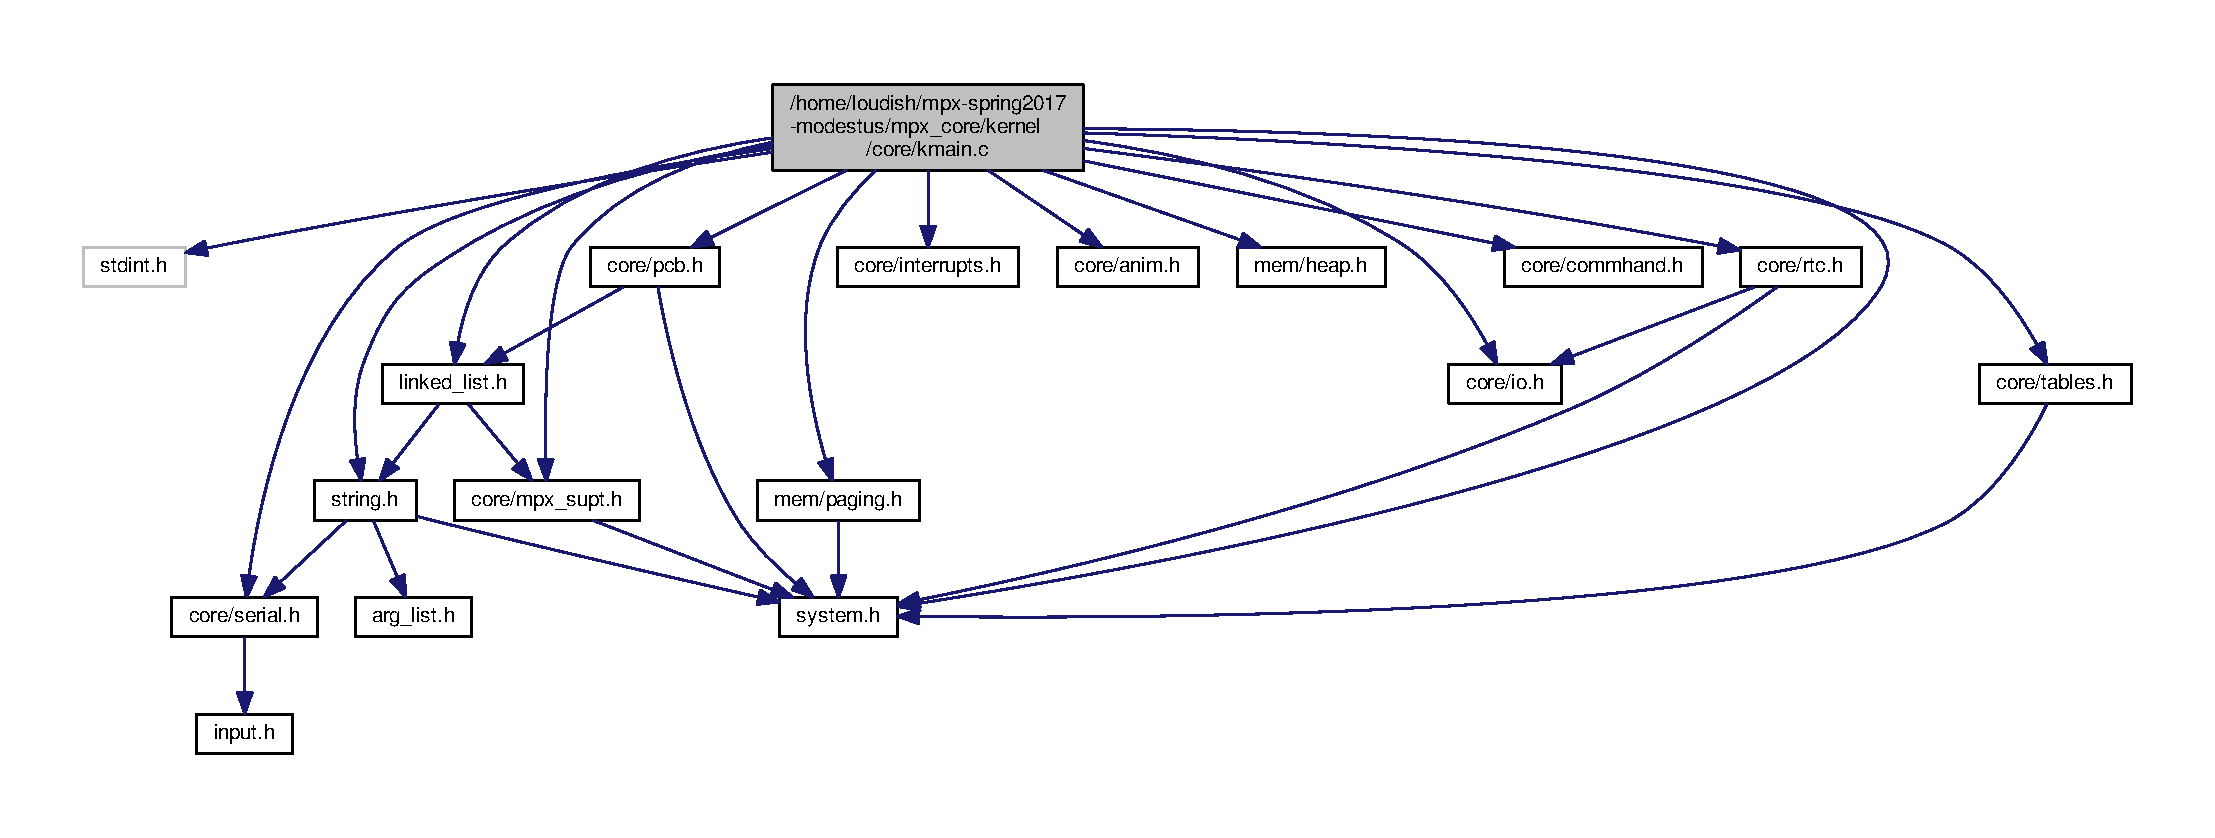
\includegraphics[width=350pt]{kmain_8c__incl}
\end{center}
\end{figure}
\subsection*{Functions}
\begin{DoxyCompactItemize}
\item 
void \hyperlink{kmain_8c_a406c20548822065e144564476378f8a1}{kmain} (void)
\end{DoxyCompactItemize}


\subsection{Function Documentation}
\index{kmain.\+c@{kmain.\+c}!kmain@{kmain}}
\index{kmain@{kmain}!kmain.\+c@{kmain.\+c}}
\subsubsection[{\texorpdfstring{kmain(void)}{kmain(void)}}]{\setlength{\rightskip}{0pt plus 5cm}void kmain (
\begin{DoxyParamCaption}
\item[{void}]{}
\end{DoxyParamCaption}
)}\hypertarget{kmain_8c_a406c20548822065e144564476378f8a1}{}\label{kmain_8c_a406c20548822065e144564476378f8a1}


Definition at line 29 of file kmain.\+c.



References atoi(), cli, C\+O\+M1, get\+\_\+date(), get\+\_\+time(), hlt, init\+\_\+commhand(), init\+\_\+gdt(), init\+\_\+idt(), init\+\_\+irq(), init\+\_\+paging(), init\+\_\+pic(), init\+P\+C\+B\+Queues(), klogv(), list\+Test(), pcb\+Test(), printf, set\+\_\+serial\+\_\+in(), set\+\_\+serial\+\_\+out(), sprintf(), start\+\_\+up\+\_\+anim(), and strcat().


\begin{DoxyCode}
30 \{
31    \textcolor{keyword}{extern} \hyperlink{system_8h_a06896e8c53f721507066c079052171f8}{uint32\_t} magic;
32    \textcolor{comment}{// Uncomment if you want to access the multiboot header}
33    \textcolor{comment}{// extern void *mbd;}
34    \textcolor{comment}{// char *boot\_loader\_name = (char*)((long*)mbd)[16];}
35 
36    \textcolor{comment}{// 0) Initialize Serial I/O and call mpx\_init}
37    \hyperlink{system_8h_abdb09834267dd4a2a0d07d43ca4d230d}{klogv}(\textcolor{stringliteral}{"Starting MPX boot sequence..."});
38    \hyperlink{system_8h_abdb09834267dd4a2a0d07d43ca4d230d}{klogv}(\textcolor{stringliteral}{"Initialized serial I/O on COM1 device..."});
39    
40 \textcolor{comment}{// nick was here 1/19/17 and added more text}
41 \textcolor{comment}{//Gio was also here on 1/20/2017}
42 
43    \textcolor{comment}{//Added: matt-g 1/17/17}
44    \hyperlink{serial_8h_ae97b87ee1f57c687e7fca6f9958e03ef}{set\_serial\_out}(\hyperlink{serial_8h_a00dbb3ab1c59e14699be9393693e2248}{COM1});
45    \hyperlink{serial_8h_a3f4008da5feabfb7e086f6673a81104b}{set\_serial\_in}(\hyperlink{serial_8h_a00dbb3ab1c59e14699be9393693e2248}{COM1}); 
46 
47     \hyperlink{anim_8h_a5bf31d96ce4c2c86dfab5440a835c457}{start\_up\_anim}();
48    
49    \textcolor{comment}{//added matt-g 1/25/17}
50     \textcolor{keywordtype}{char} buf[500];
51    \textcolor{keywordtype}{char} *testarr = (\textcolor{keywordtype}{char}*)buf;
52 
53    \textcolor{keyword}{const} \textcolor{keywordtype}{char}* toCpy = \textcolor{stringliteral}{"testetst"};
54    testarr=\hyperlink{string_8h_a8908188ae9fc2f05d993257ef001d553}{strcat}(testarr,toCpy);
55    \hyperlink{string_8h_a0f459d16901ef591acaafa4b67fd4be5}{printf}(\textcolor{stringliteral}{"-%s-%s %s %d %s %c %s"},\textcolor{stringliteral}{"testtest"},\textcolor{stringliteral}{"matt"},\textcolor{stringliteral}{"jesse"},-938,\textcolor{stringliteral}{"gio"},\textcolor{charliteral}{'l'},\textcolor{stringliteral}{"nick"});
56    \hyperlink{string_8h_a0f459d16901ef591acaafa4b67fd4be5}{printf}(\textcolor{stringliteral}{"atoi test: %d\(\backslash\)r\(\backslash\)n"}, \hyperlink{string_8h_a30670a60464f77af17dfb353353d6df8}{atoi}(\textcolor{stringliteral}{"12 4"}));
57    \textcolor{comment}{//klogv(testarr);}
58 
59    \textcolor{keywordtype}{int} seconds = 30, minutes=49, hours=5;
60    \hyperlink{rtc_8h_a35fa24488cb7eb077e8dc995729202cf}{get\_time}(&hours,&minutes,&seconds);
61    \hyperlink{string_8h_ae9cac82f3293a00d8ec8705a3fc5cf64}{sprintf}(&testarr[0], 500, \textcolor{stringliteral}{"Hours %d, Minutes %d, Seconds %d"}, hours, minutes, seconds);
62    \hyperlink{system_8h_abdb09834267dd4a2a0d07d43ca4d230d}{klogv}(testarr);
63 
64    \textcolor{keywordtype}{int} day=25, month=12, year=2016;
65    \hyperlink{rtc_8h_ab43f56447c49f42bb4baee3e59e2d1f9}{get\_date}(&day, &month, &year);
66    \hyperlink{string_8h_ae9cac82f3293a00d8ec8705a3fc5cf64}{sprintf}(&testarr[0], 500, \textcolor{stringliteral}{"Day %d, Month %d, Year %d"}, day, month, year);
67    \hyperlink{system_8h_abdb09834267dd4a2a0d07d43ca4d230d}{klogv}(testarr);
68 
69    \textcolor{comment}{// 1) Check that the boot was successful and correct when using grub}
70    \textcolor{comment}{// Comment this when booting the kernel directly using QEMU, etc.}
71    \textcolor{keywordflow}{if} ( magic != 0x2BADB002 )\{
72      \textcolor{comment}{//kpanic("Boot was not error free. Halting.");}
73    \}
74    
75    \textcolor{comment}{// 2) Descriptor Tables}
76    \hyperlink{system_8h_abdb09834267dd4a2a0d07d43ca4d230d}{klogv}(\textcolor{stringliteral}{"Initializing Global descriptor table..."});
77    \hyperlink{tables_8h_a86bb50044169930202cc403376ef40c3}{init\_gdt}(); \textcolor{comment}{//Added: matt-g 17/1/18}
78    
79    \hyperlink{system_8h_abdb09834267dd4a2a0d07d43ca4d230d}{klogv}(\textcolor{stringliteral}{"Initializing Interrupt Descriptor table.."});
80    \hyperlink{tables_8h_a35fe413107af682030ab7a4b6dff19b8}{init\_idt}();
81    
82    \hyperlink{system_8h_abdb09834267dd4a2a0d07d43ca4d230d}{klogv}(\textcolor{stringliteral}{"Initializing Programmable interrupt controller"});
83    \hyperlink{interrupts_8h_afbc0dbef6f15e2df21b38724ea38c483}{init\_pic}();
84    
85    \hyperlink{system_8h_abdb09834267dd4a2a0d07d43ca4d230d}{klogv}(\textcolor{stringliteral}{"Installing interrupts..."});
86    \hyperlink{interrupts_8h_ad17d9a8aa78440af8fc40d3fd55dbad8}{init\_irq}();
87    
88    \hyperlink{system_8h_abdb09834267dd4a2a0d07d43ca4d230d}{klogv}(\textcolor{stringliteral}{"Enabling interrupts."});
89    \hyperlink{system_8h_a68c330e94fe121eba993e5a5973c3162}{cli}();
90 
91    \textcolor{comment}{// 4) Virtual Memory}
92    \hyperlink{system_8h_abdb09834267dd4a2a0d07d43ca4d230d}{klogv}(\textcolor{stringliteral}{"Initializing virtual memory..."});
93    \hyperlink{paging_8h_a919b727f386797a8b9d8eceb5c4e7313}{init\_paging}();
94 
95    \hyperlink{system_8h_abdb09834267dd4a2a0d07d43ca4d230d}{klogv}(\textcolor{stringliteral}{"Initializing PCB Memory"});
96    \hyperlink{pcb_8h_a8649777d644ec839c0d02d966f068f45}{initPCBQueues}();
97 
98    \textcolor{comment}{// 5) Call Commhand}
99    \hyperlink{system_8h_abdb09834267dd4a2a0d07d43ca4d230d}{klogv}(\textcolor{stringliteral}{"Transferring control to commhand..."});
100 
101    \hyperlink{linked__list_8h_a0a60ac1fe6e5055de61277ac9703b13e}{listTest}();
102 
103    \hyperlink{string_8h_a0f459d16901ef591acaafa4b67fd4be5}{printf}(\textcolor{stringliteral}{"%s%s"},\textcolor{stringliteral}{"\(\backslash\)r\(\backslash\)n"},\textcolor{stringliteral}{"\(\backslash\)r\(\backslash\)n"});
104 
105    \hyperlink{pcb_8h_adc4d10af06448eb7a046bacfc2918ea2}{pcbTest}();
106 
107     \hyperlink{commhand_8h_a5f6c259a5d805f1a24d35f36cb9207d3}{init\_commhand}();
108 
109    \textcolor{comment}{// 11) System Shutdown}
110    \hyperlink{system_8h_abdb09834267dd4a2a0d07d43ca4d230d}{klogv}(\textcolor{stringliteral}{"Starting system shutdown procedure..."});
111    
112    \textcolor{comment}{/* Shutdown Procedure */}
113    \hyperlink{system_8h_abdb09834267dd4a2a0d07d43ca4d230d}{klogv}(\textcolor{stringliteral}{"Shutdown complete. You may now turn off the machine. (QEMU: C-a x)"});
114    \hyperlink{system_8h_a954b0134ce21d80f0efb22c77e821da3}{hlt}();
115 \}
\end{DoxyCode}

\hypertarget{kernel_2core_2mpx__supt_8c}{}\section{/home/loudish/mpx-\/spring2017-\/modestus/mpx\+\_\+core/kernel/core/mpx\+\_\+supt.c File Reference}
\label{kernel_2core_2mpx__supt_8c}\index{/home/loudish/mpx-\/spring2017-\/modestus/mpx\+\_\+core/kernel/core/mpx\+\_\+supt.\+c@{/home/loudish/mpx-\/spring2017-\/modestus/mpx\+\_\+core/kernel/core/mpx\+\_\+supt.\+c}}
{\ttfamily \#include $<$core/mpx\+\_\+supt.\+h$>$}\\*
{\ttfamily \#include $<$mem/heap.\+h$>$}\\*
Include dependency graph for mpx\+\_\+supt.\+c\+:\nopagebreak
\begin{figure}[H]
\begin{center}
\leavevmode
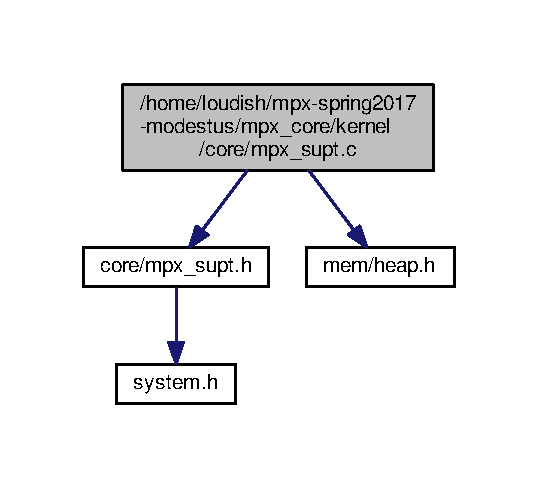
\includegraphics[width=258pt]{kernel_2core_2mpx__supt_8c__incl}
\end{center}
\end{figure}
\subsection*{Functions}
\begin{DoxyCompactItemize}
\item 
int \hyperlink{kernel_2core_2mpx__supt_8c_afb6ff5e2e9bdde9d8971a497b6fe38ae}{sys\+\_\+req} (int op\+\_\+code)
\item 
void \hyperlink{kernel_2core_2mpx__supt_8c_a53332c6a3107a4feed6e2e79690a6ffa}{mpx\+\_\+init} (int cur\+\_\+mod)
\item 
void \hyperlink{kernel_2core_2mpx__supt_8c_a4a28bb188c9fed51228c46980b20e605}{sys\+\_\+set\+\_\+malloc} (\hyperlink{system_8h_a757de76cafbcddaac0d1632902fe4cb8}{u32int}($\ast$func)(\hyperlink{system_8h_a757de76cafbcddaac0d1632902fe4cb8}{u32int}))
\item 
void \hyperlink{kernel_2core_2mpx__supt_8c_a2463d934fa39601c275a3ade8afd18bc}{sys\+\_\+set\+\_\+free} (int($\ast$func)(void $\ast$))
\item 
void $\ast$ \hyperlink{kernel_2core_2mpx__supt_8c_a61adad2abba0a3a225c2290b3de1fe93}{sys\+\_\+alloc\+\_\+mem} (\hyperlink{system_8h_a757de76cafbcddaac0d1632902fe4cb8}{u32int} size)
\item 
int \hyperlink{kernel_2core_2mpx__supt_8c_a950663d39dbb073c9dff9cf3b5d3392c}{sys\+\_\+free\+\_\+mem} (void $\ast$ptr)
\item 
void \hyperlink{kernel_2core_2mpx__supt_8c_a83abbeda22fc5e6c2b35523b64199c1c}{idle} ()
\end{DoxyCompactItemize}
\subsection*{Variables}
\begin{DoxyCompactItemize}
\item 
\hyperlink{structparam}{param} \hyperlink{kernel_2core_2mpx__supt_8c_a3b4b77494d0fad58939896ddc5290c99}{params}
\item 
int \hyperlink{kernel_2core_2mpx__supt_8c_a3d19c725b7f9f45e9da97a79ca6a4737}{current\+\_\+module} = -\/1
\item 
\hyperlink{system_8h_a757de76cafbcddaac0d1632902fe4cb8}{u32int}($\ast$ \hyperlink{kernel_2core_2mpx__supt_8c_a421e2b48efb5facc71d16979252710e2}{student\+\_\+malloc} )(\hyperlink{system_8h_a757de76cafbcddaac0d1632902fe4cb8}{u32int})
\item 
int($\ast$ \hyperlink{kernel_2core_2mpx__supt_8c_a19c47c02b0338bc13716d98305bb8a34}{student\+\_\+free} )(void $\ast$)
\end{DoxyCompactItemize}


\subsection{Function Documentation}
\index{kernel/core/mpx\+\_\+supt.\+c@{kernel/core/mpx\+\_\+supt.\+c}!idle@{idle}}
\index{idle@{idle}!kernel/core/mpx\+\_\+supt.\+c@{kernel/core/mpx\+\_\+supt.\+c}}
\subsubsection[{\texorpdfstring{idle()}{idle()}}]{\setlength{\rightskip}{0pt plus 5cm}void idle (
\begin{DoxyParamCaption}
{}
\end{DoxyParamCaption}
)}\hypertarget{kernel_2core_2mpx__supt_8c_a83abbeda22fc5e6c2b35523b64199c1c}{}\label{kernel_2core_2mpx__supt_8c_a83abbeda22fc5e6c2b35523b64199c1c}


Definition at line 47 of file mpx\+\_\+supt.\+c.


\begin{DoxyCode}
48 \{
49   \textcolor{keywordflow}{while}(1)\{
50     \hyperlink{kernel_2core_2mpx__supt_8c_afb6ff5e2e9bdde9d8971a497b6fe38ae}{sys\_req}(\hyperlink{include_2core_2mpx__supt_8h_a9c21a7caee326d7803b94ae1952b27ca}{IDLE});
51   \}
52 \}
\end{DoxyCode}
\index{kernel/core/mpx\+\_\+supt.\+c@{kernel/core/mpx\+\_\+supt.\+c}!mpx\+\_\+init@{mpx\+\_\+init}}
\index{mpx\+\_\+init@{mpx\+\_\+init}!kernel/core/mpx\+\_\+supt.\+c@{kernel/core/mpx\+\_\+supt.\+c}}
\subsubsection[{\texorpdfstring{mpx\+\_\+init(int cur\+\_\+mod)}{mpx_init(int cur_mod)}}]{\setlength{\rightskip}{0pt plus 5cm}void mpx\+\_\+init (
\begin{DoxyParamCaption}
\item[{int}]{cur\+\_\+mod}
\end{DoxyParamCaption}
)}\hypertarget{kernel_2core_2mpx__supt_8c_a53332c6a3107a4feed6e2e79690a6ffa}{}\label{kernel_2core_2mpx__supt_8c_a53332c6a3107a4feed6e2e79690a6ffa}


Definition at line 16 of file mpx\+\_\+supt.\+c.


\begin{DoxyCode}
17 \{
18   \hyperlink{kernel_2core_2mpx__supt_8c_a3d19c725b7f9f45e9da97a79ca6a4737}{current\_module} = cur\_mod;
19 \}
\end{DoxyCode}
\index{kernel/core/mpx\+\_\+supt.\+c@{kernel/core/mpx\+\_\+supt.\+c}!sys\+\_\+alloc\+\_\+mem@{sys\+\_\+alloc\+\_\+mem}}
\index{sys\+\_\+alloc\+\_\+mem@{sys\+\_\+alloc\+\_\+mem}!kernel/core/mpx\+\_\+supt.\+c@{kernel/core/mpx\+\_\+supt.\+c}}
\subsubsection[{\texorpdfstring{sys\+\_\+alloc\+\_\+mem(u32int size)}{sys_alloc_mem(u32int size)}}]{\setlength{\rightskip}{0pt plus 5cm}void$\ast$ sys\+\_\+alloc\+\_\+mem (
\begin{DoxyParamCaption}
\item[{{\bf u32int}}]{size}
\end{DoxyParamCaption}
)}\hypertarget{kernel_2core_2mpx__supt_8c_a61adad2abba0a3a225c2290b3de1fe93}{}\label{kernel_2core_2mpx__supt_8c_a61adad2abba0a3a225c2290b3de1fe93}


Definition at line 31 of file mpx\+\_\+supt.\+c.


\begin{DoxyCode}
32 \{
33   \textcolor{keywordflow}{if} (\hyperlink{kernel_2core_2mpx__supt_8c_a3d19c725b7f9f45e9da97a79ca6a4737}{current\_module} < \hyperlink{include_2core_2mpx__supt_8h_a68745bb3b58fd02dcee2cad3b2331def}{MODULE\_R5})
34     \textcolor{keywordflow}{return} (\textcolor{keywordtype}{void} *) \hyperlink{heap_8h_a15d6a52c5c080c8c7ffc73e336d8e574}{kmalloc}(size);
35   \textcolor{keywordflow}{else}
36     \textcolor{keywordflow}{return} (\textcolor{keywordtype}{void} *) (*student\_malloc)(size);
37 \}
\end{DoxyCode}
\index{kernel/core/mpx\+\_\+supt.\+c@{kernel/core/mpx\+\_\+supt.\+c}!sys\+\_\+free\+\_\+mem@{sys\+\_\+free\+\_\+mem}}
\index{sys\+\_\+free\+\_\+mem@{sys\+\_\+free\+\_\+mem}!kernel/core/mpx\+\_\+supt.\+c@{kernel/core/mpx\+\_\+supt.\+c}}
\subsubsection[{\texorpdfstring{sys\+\_\+free\+\_\+mem(void $\ast$ptr)}{sys_free_mem(void *ptr)}}]{\setlength{\rightskip}{0pt plus 5cm}int sys\+\_\+free\+\_\+mem (
\begin{DoxyParamCaption}
\item[{void $\ast$}]{ptr}
\end{DoxyParamCaption}
)}\hypertarget{kernel_2core_2mpx__supt_8c_a950663d39dbb073c9dff9cf3b5d3392c}{}\label{kernel_2core_2mpx__supt_8c_a950663d39dbb073c9dff9cf3b5d3392c}


Definition at line 39 of file mpx\+\_\+supt.\+c.


\begin{DoxyCode}
40 \{
41   \textcolor{keywordflow}{if} (\hyperlink{kernel_2core_2mpx__supt_8c_a3d19c725b7f9f45e9da97a79ca6a4737}{current\_module} >= \hyperlink{include_2core_2mpx__supt_8h_a68745bb3b58fd02dcee2cad3b2331def}{MODULE\_R5})
42     \textcolor{keywordflow}{return} (*\hyperlink{kernel_2core_2mpx__supt_8c_a19c47c02b0338bc13716d98305bb8a34}{student\_free})(ptr);
43   \textcolor{comment}{// otherwise we don't free anything}
44   \textcolor{keywordflow}{return} -1;
45 \}
\end{DoxyCode}
\index{kernel/core/mpx\+\_\+supt.\+c@{kernel/core/mpx\+\_\+supt.\+c}!sys\+\_\+req@{sys\+\_\+req}}
\index{sys\+\_\+req@{sys\+\_\+req}!kernel/core/mpx\+\_\+supt.\+c@{kernel/core/mpx\+\_\+supt.\+c}}
\subsubsection[{\texorpdfstring{sys\+\_\+req(int op\+\_\+code)}{sys_req(int op_code)}}]{\setlength{\rightskip}{0pt plus 5cm}int sys\+\_\+req (
\begin{DoxyParamCaption}
\item[{int}]{op\+\_\+code}
\end{DoxyParamCaption}
)}\hypertarget{kernel_2core_2mpx__supt_8c_afb6ff5e2e9bdde9d8971a497b6fe38ae}{}\label{kernel_2core_2mpx__supt_8c_afb6ff5e2e9bdde9d8971a497b6fe38ae}


Definition at line 9 of file mpx\+\_\+supt.\+c.



Referenced by idle().


\begin{DoxyCode}
10 \{
11   \hyperlink{kernel_2core_2mpx__supt_8c_a3b4b77494d0fad58939896ddc5290c99}{params}.\hyperlink{structparam_a81c8b24055c2908ebe480598aba6044c}{op\_code} = op\_code;
12   \textcolor{keyword}{asm} \textcolor{keyword}{volatile} (\textcolor{stringliteral}{"int $60"});
13   \textcolor{keywordflow}{return} 0;
14 \}
\end{DoxyCode}
\index{kernel/core/mpx\+\_\+supt.\+c@{kernel/core/mpx\+\_\+supt.\+c}!sys\+\_\+set\+\_\+free@{sys\+\_\+set\+\_\+free}}
\index{sys\+\_\+set\+\_\+free@{sys\+\_\+set\+\_\+free}!kernel/core/mpx\+\_\+supt.\+c@{kernel/core/mpx\+\_\+supt.\+c}}
\subsubsection[{\texorpdfstring{sys\+\_\+set\+\_\+free(int($\ast$func)(void $\ast$))}{sys_set_free(int(*func)(void *))}}]{\setlength{\rightskip}{0pt plus 5cm}void sys\+\_\+set\+\_\+free (
\begin{DoxyParamCaption}
\item[{int($\ast$)(void $\ast$)}]{func}
\end{DoxyParamCaption}
)}\hypertarget{kernel_2core_2mpx__supt_8c_a2463d934fa39601c275a3ade8afd18bc}{}\label{kernel_2core_2mpx__supt_8c_a2463d934fa39601c275a3ade8afd18bc}


Definition at line 26 of file mpx\+\_\+supt.\+c.


\begin{DoxyCode}
27 \{
28   \hyperlink{kernel_2core_2mpx__supt_8c_a19c47c02b0338bc13716d98305bb8a34}{student\_free} = func;
29 \}
\end{DoxyCode}
\index{kernel/core/mpx\+\_\+supt.\+c@{kernel/core/mpx\+\_\+supt.\+c}!sys\+\_\+set\+\_\+malloc@{sys\+\_\+set\+\_\+malloc}}
\index{sys\+\_\+set\+\_\+malloc@{sys\+\_\+set\+\_\+malloc}!kernel/core/mpx\+\_\+supt.\+c@{kernel/core/mpx\+\_\+supt.\+c}}
\subsubsection[{\texorpdfstring{sys\+\_\+set\+\_\+malloc(u32int($\ast$func)(u32int))}{sys_set_malloc(u32int(*func)(u32int))}}]{\setlength{\rightskip}{0pt plus 5cm}void sys\+\_\+set\+\_\+malloc (
\begin{DoxyParamCaption}
\item[{{\bf u32int}($\ast$)({\bf u32int})}]{func}
\end{DoxyParamCaption}
)}\hypertarget{kernel_2core_2mpx__supt_8c_a4a28bb188c9fed51228c46980b20e605}{}\label{kernel_2core_2mpx__supt_8c_a4a28bb188c9fed51228c46980b20e605}


Definition at line 21 of file mpx\+\_\+supt.\+c.


\begin{DoxyCode}
22 \{
23   \hyperlink{kernel_2core_2mpx__supt_8c_a421e2b48efb5facc71d16979252710e2}{student\_malloc} = func;
24 \}
\end{DoxyCode}


\subsection{Variable Documentation}
\index{kernel/core/mpx\+\_\+supt.\+c@{kernel/core/mpx\+\_\+supt.\+c}!current\+\_\+module@{current\+\_\+module}}
\index{current\+\_\+module@{current\+\_\+module}!kernel/core/mpx\+\_\+supt.\+c@{kernel/core/mpx\+\_\+supt.\+c}}
\subsubsection[{\texorpdfstring{current\+\_\+module}{current_module}}]{\setlength{\rightskip}{0pt plus 5cm}int current\+\_\+module = -\/1}\hypertarget{kernel_2core_2mpx__supt_8c_a3d19c725b7f9f45e9da97a79ca6a4737}{}\label{kernel_2core_2mpx__supt_8c_a3d19c725b7f9f45e9da97a79ca6a4737}


Definition at line 5 of file mpx\+\_\+supt.\+c.



Referenced by mpx\+\_\+init(), sys\+\_\+alloc\+\_\+mem(), and sys\+\_\+free\+\_\+mem().

\index{kernel/core/mpx\+\_\+supt.\+c@{kernel/core/mpx\+\_\+supt.\+c}!params@{params}}
\index{params@{params}!kernel/core/mpx\+\_\+supt.\+c@{kernel/core/mpx\+\_\+supt.\+c}}
\subsubsection[{\texorpdfstring{params}{params}}]{\setlength{\rightskip}{0pt plus 5cm}{\bf param} params}\hypertarget{kernel_2core_2mpx__supt_8c_a3b4b77494d0fad58939896ddc5290c99}{}\label{kernel_2core_2mpx__supt_8c_a3b4b77494d0fad58939896ddc5290c99}


Definition at line 4 of file mpx\+\_\+supt.\+c.

\index{kernel/core/mpx\+\_\+supt.\+c@{kernel/core/mpx\+\_\+supt.\+c}!student\+\_\+free@{student\+\_\+free}}
\index{student\+\_\+free@{student\+\_\+free}!kernel/core/mpx\+\_\+supt.\+c@{kernel/core/mpx\+\_\+supt.\+c}}
\subsubsection[{\texorpdfstring{student\+\_\+free}{student_free}}]{\setlength{\rightskip}{0pt plus 5cm}int($\ast$ student\+\_\+free) (void $\ast$)}\hypertarget{kernel_2core_2mpx__supt_8c_a19c47c02b0338bc13716d98305bb8a34}{}\label{kernel_2core_2mpx__supt_8c_a19c47c02b0338bc13716d98305bb8a34}


Definition at line 7 of file mpx\+\_\+supt.\+c.



Referenced by sys\+\_\+free\+\_\+mem(), and sys\+\_\+set\+\_\+free().

\index{kernel/core/mpx\+\_\+supt.\+c@{kernel/core/mpx\+\_\+supt.\+c}!student\+\_\+malloc@{student\+\_\+malloc}}
\index{student\+\_\+malloc@{student\+\_\+malloc}!kernel/core/mpx\+\_\+supt.\+c@{kernel/core/mpx\+\_\+supt.\+c}}
\subsubsection[{\texorpdfstring{student\+\_\+malloc}{student_malloc}}]{\setlength{\rightskip}{0pt plus 5cm}{\bf u32int}($\ast$ student\+\_\+malloc) ({\bf u32int})}\hypertarget{kernel_2core_2mpx__supt_8c_a421e2b48efb5facc71d16979252710e2}{}\label{kernel_2core_2mpx__supt_8c_a421e2b48efb5facc71d16979252710e2}


Definition at line 6 of file mpx\+\_\+supt.\+c.



Referenced by sys\+\_\+set\+\_\+malloc().


\hypertarget{modules_2mpx__supt_8c}{}\section{/home/loudish/mpx-\/spring2017-\/modestus/mpx\+\_\+core/modules/mpx\+\_\+supt.c File Reference}
\label{modules_2mpx__supt_8c}\index{/home/loudish/mpx-\/spring2017-\/modestus/mpx\+\_\+core/modules/mpx\+\_\+supt.\+c@{/home/loudish/mpx-\/spring2017-\/modestus/mpx\+\_\+core/modules/mpx\+\_\+supt.\+c}}
{\ttfamily \#include \char`\"{}mpx\+\_\+supt.\+h\char`\"{}}\\*
{\ttfamily \#include $<$mem/heap.\+h$>$}\\*
Include dependency graph for mpx\+\_\+supt.\+c\+:\nopagebreak
\begin{figure}[H]
\begin{center}
\leavevmode
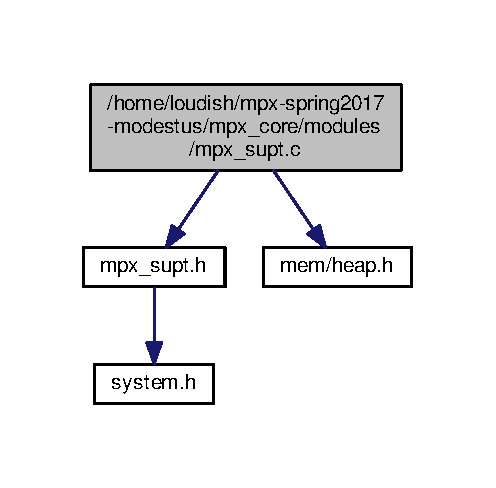
\includegraphics[width=238pt]{modules_2mpx__supt_8c__incl}
\end{center}
\end{figure}
\subsection*{Functions}
\begin{DoxyCompactItemize}
\item 
int \hyperlink{modules_2mpx__supt_8c_afb6ff5e2e9bdde9d8971a497b6fe38ae}{sys\+\_\+req} (int op\+\_\+code)
\item 
void \hyperlink{modules_2mpx__supt_8c_a53332c6a3107a4feed6e2e79690a6ffa}{mpx\+\_\+init} (int cur\+\_\+mod)
\item 
void \hyperlink{modules_2mpx__supt_8c_a4a28bb188c9fed51228c46980b20e605}{sys\+\_\+set\+\_\+malloc} (\hyperlink{system_8h_a757de76cafbcddaac0d1632902fe4cb8}{u32int}($\ast$func)(\hyperlink{system_8h_a757de76cafbcddaac0d1632902fe4cb8}{u32int}))
\item 
void \hyperlink{modules_2mpx__supt_8c_a2463d934fa39601c275a3ade8afd18bc}{sys\+\_\+set\+\_\+free} (int($\ast$func)(void $\ast$))
\item 
void $\ast$ \hyperlink{modules_2mpx__supt_8c_a61adad2abba0a3a225c2290b3de1fe93}{sys\+\_\+alloc\+\_\+mem} (\hyperlink{system_8h_a757de76cafbcddaac0d1632902fe4cb8}{u32int} size)
\item 
int \hyperlink{modules_2mpx__supt_8c_a950663d39dbb073c9dff9cf3b5d3392c}{sys\+\_\+free\+\_\+mem} (void $\ast$ptr)
\item 
void \hyperlink{modules_2mpx__supt_8c_a83abbeda22fc5e6c2b35523b64199c1c}{idle} ()
\end{DoxyCompactItemize}
\subsection*{Variables}
\begin{DoxyCompactItemize}
\item 
\hyperlink{structparam}{param} \hyperlink{modules_2mpx__supt_8c_a3b4b77494d0fad58939896ddc5290c99}{params}
\item 
int \hyperlink{modules_2mpx__supt_8c_a3d19c725b7f9f45e9da97a79ca6a4737}{current\+\_\+module} = -\/1
\item 
\hyperlink{system_8h_a757de76cafbcddaac0d1632902fe4cb8}{u32int}($\ast$ \hyperlink{modules_2mpx__supt_8c_a421e2b48efb5facc71d16979252710e2}{student\+\_\+malloc} )(\hyperlink{system_8h_a757de76cafbcddaac0d1632902fe4cb8}{u32int})
\item 
int($\ast$ \hyperlink{modules_2mpx__supt_8c_a19c47c02b0338bc13716d98305bb8a34}{student\+\_\+free} )(void $\ast$)
\end{DoxyCompactItemize}


\subsection{Function Documentation}
\index{modules/mpx\+\_\+supt.\+c@{modules/mpx\+\_\+supt.\+c}!idle@{idle}}
\index{idle@{idle}!modules/mpx\+\_\+supt.\+c@{modules/mpx\+\_\+supt.\+c}}
\subsubsection[{\texorpdfstring{idle()}{idle()}}]{\setlength{\rightskip}{0pt plus 5cm}void idle (
\begin{DoxyParamCaption}
{}
\end{DoxyParamCaption}
)}\hypertarget{modules_2mpx__supt_8c_a83abbeda22fc5e6c2b35523b64199c1c}{}\label{modules_2mpx__supt_8c_a83abbeda22fc5e6c2b35523b64199c1c}


Definition at line 47 of file mpx\+\_\+supt.\+c.



References I\+D\+LE, and sys\+\_\+req().


\begin{DoxyCode}
48 \{
49   \textcolor{keywordflow}{while}(1)\{
50     \hyperlink{kernel_2core_2mpx__supt_8c_afb6ff5e2e9bdde9d8971a497b6fe38ae}{sys\_req}(\hyperlink{include_2core_2mpx__supt_8h_a9c21a7caee326d7803b94ae1952b27ca}{IDLE});
51   \}
52 \}
\end{DoxyCode}
\index{modules/mpx\+\_\+supt.\+c@{modules/mpx\+\_\+supt.\+c}!mpx\+\_\+init@{mpx\+\_\+init}}
\index{mpx\+\_\+init@{mpx\+\_\+init}!modules/mpx\+\_\+supt.\+c@{modules/mpx\+\_\+supt.\+c}}
\subsubsection[{\texorpdfstring{mpx\+\_\+init(int cur\+\_\+mod)}{mpx_init(int cur_mod)}}]{\setlength{\rightskip}{0pt plus 5cm}void mpx\+\_\+init (
\begin{DoxyParamCaption}
\item[{int}]{cur\+\_\+mod}
\end{DoxyParamCaption}
)}\hypertarget{modules_2mpx__supt_8c_a53332c6a3107a4feed6e2e79690a6ffa}{}\label{modules_2mpx__supt_8c_a53332c6a3107a4feed6e2e79690a6ffa}


Definition at line 16 of file mpx\+\_\+supt.\+c.



References current\+\_\+module.


\begin{DoxyCode}
17 \{
18   \hyperlink{kernel_2core_2mpx__supt_8c_a3d19c725b7f9f45e9da97a79ca6a4737}{current\_module} = cur\_mod;
19 \}
\end{DoxyCode}
\index{modules/mpx\+\_\+supt.\+c@{modules/mpx\+\_\+supt.\+c}!sys\+\_\+alloc\+\_\+mem@{sys\+\_\+alloc\+\_\+mem}}
\index{sys\+\_\+alloc\+\_\+mem@{sys\+\_\+alloc\+\_\+mem}!modules/mpx\+\_\+supt.\+c@{modules/mpx\+\_\+supt.\+c}}
\subsubsection[{\texorpdfstring{sys\+\_\+alloc\+\_\+mem(u32int size)}{sys_alloc_mem(u32int size)}}]{\setlength{\rightskip}{0pt plus 5cm}void$\ast$ sys\+\_\+alloc\+\_\+mem (
\begin{DoxyParamCaption}
\item[{{\bf u32int}}]{size}
\end{DoxyParamCaption}
)}\hypertarget{modules_2mpx__supt_8c_a61adad2abba0a3a225c2290b3de1fe93}{}\label{modules_2mpx__supt_8c_a61adad2abba0a3a225c2290b3de1fe93}


Definition at line 31 of file mpx\+\_\+supt.\+c.



References current\+\_\+module, kmalloc(), and M\+O\+D\+U\+L\+E\+\_\+\+R5.



Referenced by allocate\+P\+C\+B(), and make\+New\+Node().


\begin{DoxyCode}
32 \{
33   \textcolor{keywordflow}{if} (\hyperlink{kernel_2core_2mpx__supt_8c_a3d19c725b7f9f45e9da97a79ca6a4737}{current\_module} < \hyperlink{include_2core_2mpx__supt_8h_a68745bb3b58fd02dcee2cad3b2331def}{MODULE\_R5})
34     \textcolor{keywordflow}{return} (\textcolor{keywordtype}{void} *) \hyperlink{heap_8h_a15d6a52c5c080c8c7ffc73e336d8e574}{kmalloc}(size);
35   \textcolor{keywordflow}{else}
36     \textcolor{keywordflow}{return} (\textcolor{keywordtype}{void} *) (*student\_malloc)(size);
37 \}
\end{DoxyCode}
\index{modules/mpx\+\_\+supt.\+c@{modules/mpx\+\_\+supt.\+c}!sys\+\_\+free\+\_\+mem@{sys\+\_\+free\+\_\+mem}}
\index{sys\+\_\+free\+\_\+mem@{sys\+\_\+free\+\_\+mem}!modules/mpx\+\_\+supt.\+c@{modules/mpx\+\_\+supt.\+c}}
\subsubsection[{\texorpdfstring{sys\+\_\+free\+\_\+mem(void $\ast$ptr)}{sys_free_mem(void *ptr)}}]{\setlength{\rightskip}{0pt plus 5cm}int sys\+\_\+free\+\_\+mem (
\begin{DoxyParamCaption}
\item[{void $\ast$}]{ptr}
\end{DoxyParamCaption}
)}\hypertarget{modules_2mpx__supt_8c_a950663d39dbb073c9dff9cf3b5d3392c}{}\label{modules_2mpx__supt_8c_a950663d39dbb073c9dff9cf3b5d3392c}


Definition at line 39 of file mpx\+\_\+supt.\+c.



References current\+\_\+module, M\+O\+D\+U\+L\+E\+\_\+\+R5, and student\+\_\+free.



Referenced by free\+P\+C\+B().


\begin{DoxyCode}
40 \{
41   \textcolor{keywordflow}{if} (\hyperlink{kernel_2core_2mpx__supt_8c_a3d19c725b7f9f45e9da97a79ca6a4737}{current\_module} >= \hyperlink{include_2core_2mpx__supt_8h_a68745bb3b58fd02dcee2cad3b2331def}{MODULE\_R5})
42     \textcolor{keywordflow}{return} (*\hyperlink{kernel_2core_2mpx__supt_8c_a19c47c02b0338bc13716d98305bb8a34}{student\_free})(ptr);
43   \textcolor{comment}{// otherwise we don't free anything}
44   \textcolor{keywordflow}{return} -1;
45 \}
\end{DoxyCode}
\index{modules/mpx\+\_\+supt.\+c@{modules/mpx\+\_\+supt.\+c}!sys\+\_\+req@{sys\+\_\+req}}
\index{sys\+\_\+req@{sys\+\_\+req}!modules/mpx\+\_\+supt.\+c@{modules/mpx\+\_\+supt.\+c}}
\subsubsection[{\texorpdfstring{sys\+\_\+req(int op\+\_\+code)}{sys_req(int op_code)}}]{\setlength{\rightskip}{0pt plus 5cm}int sys\+\_\+req (
\begin{DoxyParamCaption}
\item[{int}]{op\+\_\+code}
\end{DoxyParamCaption}
)}\hypertarget{modules_2mpx__supt_8c_afb6ff5e2e9bdde9d8971a497b6fe38ae}{}\label{modules_2mpx__supt_8c_afb6ff5e2e9bdde9d8971a497b6fe38ae}


Definition at line 9 of file mpx\+\_\+supt.\+c.



References param\+::op\+\_\+code.


\begin{DoxyCode}
10 \{
11   \hyperlink{kernel_2core_2mpx__supt_8c_a3b4b77494d0fad58939896ddc5290c99}{params}.\hyperlink{structparam_a81c8b24055c2908ebe480598aba6044c}{op\_code} = op\_code;
12   \textcolor{keyword}{asm} \textcolor{keyword}{volatile} (\textcolor{stringliteral}{"int $60"});
13   \textcolor{keywordflow}{return} 0;
14 \}
\end{DoxyCode}
\index{modules/mpx\+\_\+supt.\+c@{modules/mpx\+\_\+supt.\+c}!sys\+\_\+set\+\_\+free@{sys\+\_\+set\+\_\+free}}
\index{sys\+\_\+set\+\_\+free@{sys\+\_\+set\+\_\+free}!modules/mpx\+\_\+supt.\+c@{modules/mpx\+\_\+supt.\+c}}
\subsubsection[{\texorpdfstring{sys\+\_\+set\+\_\+free(int($\ast$func)(void $\ast$))}{sys_set_free(int(*func)(void *))}}]{\setlength{\rightskip}{0pt plus 5cm}void sys\+\_\+set\+\_\+free (
\begin{DoxyParamCaption}
\item[{int($\ast$)(void $\ast$)}]{func}
\end{DoxyParamCaption}
)}\hypertarget{modules_2mpx__supt_8c_a2463d934fa39601c275a3ade8afd18bc}{}\label{modules_2mpx__supt_8c_a2463d934fa39601c275a3ade8afd18bc}


Definition at line 26 of file mpx\+\_\+supt.\+c.



References student\+\_\+free.


\begin{DoxyCode}
27 \{
28   \hyperlink{kernel_2core_2mpx__supt_8c_a19c47c02b0338bc13716d98305bb8a34}{student\_free} = func;
29 \}
\end{DoxyCode}
\index{modules/mpx\+\_\+supt.\+c@{modules/mpx\+\_\+supt.\+c}!sys\+\_\+set\+\_\+malloc@{sys\+\_\+set\+\_\+malloc}}
\index{sys\+\_\+set\+\_\+malloc@{sys\+\_\+set\+\_\+malloc}!modules/mpx\+\_\+supt.\+c@{modules/mpx\+\_\+supt.\+c}}
\subsubsection[{\texorpdfstring{sys\+\_\+set\+\_\+malloc(u32int($\ast$func)(u32int))}{sys_set_malloc(u32int(*func)(u32int))}}]{\setlength{\rightskip}{0pt plus 5cm}void sys\+\_\+set\+\_\+malloc (
\begin{DoxyParamCaption}
\item[{{\bf u32int}($\ast$)({\bf u32int})}]{func}
\end{DoxyParamCaption}
)}\hypertarget{modules_2mpx__supt_8c_a4a28bb188c9fed51228c46980b20e605}{}\label{modules_2mpx__supt_8c_a4a28bb188c9fed51228c46980b20e605}


Definition at line 21 of file mpx\+\_\+supt.\+c.



References student\+\_\+malloc.


\begin{DoxyCode}
22 \{
23   \hyperlink{kernel_2core_2mpx__supt_8c_a421e2b48efb5facc71d16979252710e2}{student\_malloc} = func;
24 \}
\end{DoxyCode}


\subsection{Variable Documentation}
\index{modules/mpx\+\_\+supt.\+c@{modules/mpx\+\_\+supt.\+c}!current\+\_\+module@{current\+\_\+module}}
\index{current\+\_\+module@{current\+\_\+module}!modules/mpx\+\_\+supt.\+c@{modules/mpx\+\_\+supt.\+c}}
\subsubsection[{\texorpdfstring{current\+\_\+module}{current_module}}]{\setlength{\rightskip}{0pt plus 5cm}int current\+\_\+module = -\/1}\hypertarget{modules_2mpx__supt_8c_a3d19c725b7f9f45e9da97a79ca6a4737}{}\label{modules_2mpx__supt_8c_a3d19c725b7f9f45e9da97a79ca6a4737}


Definition at line 5 of file mpx\+\_\+supt.\+c.

\index{modules/mpx\+\_\+supt.\+c@{modules/mpx\+\_\+supt.\+c}!params@{params}}
\index{params@{params}!modules/mpx\+\_\+supt.\+c@{modules/mpx\+\_\+supt.\+c}}
\subsubsection[{\texorpdfstring{params}{params}}]{\setlength{\rightskip}{0pt plus 5cm}{\bf param} params}\hypertarget{modules_2mpx__supt_8c_a3b4b77494d0fad58939896ddc5290c99}{}\label{modules_2mpx__supt_8c_a3b4b77494d0fad58939896ddc5290c99}


Definition at line 4 of file mpx\+\_\+supt.\+c.

\index{modules/mpx\+\_\+supt.\+c@{modules/mpx\+\_\+supt.\+c}!student\+\_\+free@{student\+\_\+free}}
\index{student\+\_\+free@{student\+\_\+free}!modules/mpx\+\_\+supt.\+c@{modules/mpx\+\_\+supt.\+c}}
\subsubsection[{\texorpdfstring{student\+\_\+free}{student_free}}]{\setlength{\rightskip}{0pt plus 5cm}int($\ast$ student\+\_\+free) (void $\ast$)}\hypertarget{modules_2mpx__supt_8c_a19c47c02b0338bc13716d98305bb8a34}{}\label{modules_2mpx__supt_8c_a19c47c02b0338bc13716d98305bb8a34}


Definition at line 7 of file mpx\+\_\+supt.\+c.

\index{modules/mpx\+\_\+supt.\+c@{modules/mpx\+\_\+supt.\+c}!student\+\_\+malloc@{student\+\_\+malloc}}
\index{student\+\_\+malloc@{student\+\_\+malloc}!modules/mpx\+\_\+supt.\+c@{modules/mpx\+\_\+supt.\+c}}
\subsubsection[{\texorpdfstring{student\+\_\+malloc}{student_malloc}}]{\setlength{\rightskip}{0pt plus 5cm}{\bf u32int}($\ast$ student\+\_\+malloc) ({\bf u32int})}\hypertarget{modules_2mpx__supt_8c_a421e2b48efb5facc71d16979252710e2}{}\label{modules_2mpx__supt_8c_a421e2b48efb5facc71d16979252710e2}


Definition at line 6 of file mpx\+\_\+supt.\+c.


\hypertarget{pcb_8c}{}\section{/home/loudish/mpx-\/spring2017-\/modestus/mpx\+\_\+core/kernel/core/pcb.c File Reference}
\label{pcb_8c}\index{/home/loudish/mpx-\/spring2017-\/modestus/mpx\+\_\+core/kernel/core/pcb.\+c@{/home/loudish/mpx-\/spring2017-\/modestus/mpx\+\_\+core/kernel/core/pcb.\+c}}
{\ttfamily \#include $<$core/pcb.\+h$>$}\\*
Include dependency graph for pcb.\+c\+:\nopagebreak
\begin{figure}[H]
\begin{center}
\leavevmode
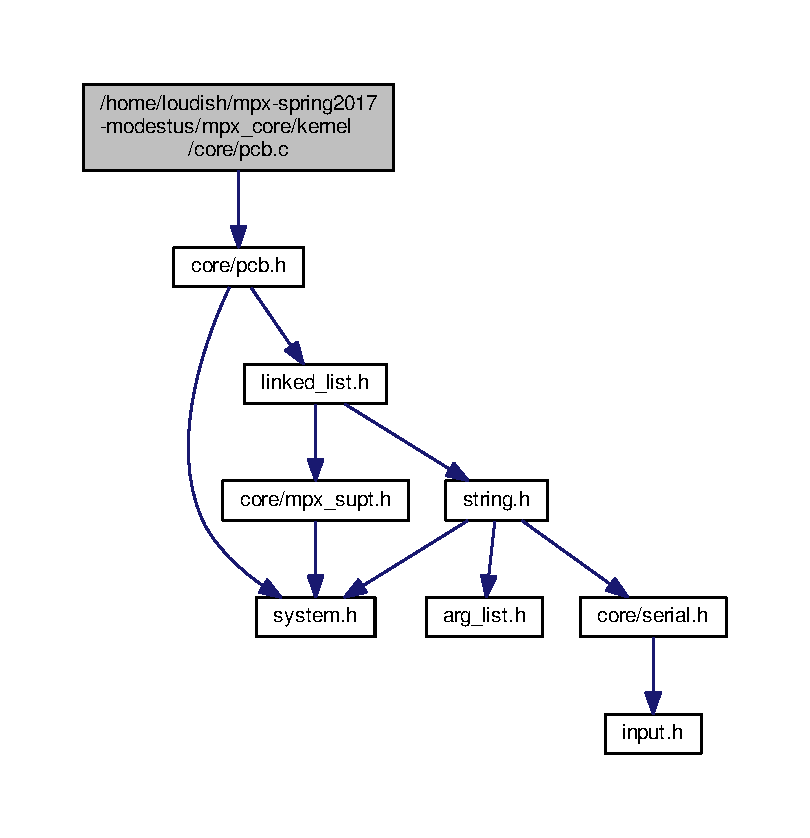
\includegraphics[width=350pt]{pcb_8c__incl}
\end{center}
\end{figure}
\subsection*{Functions}
\begin{DoxyCompactItemize}
\item 
\hyperlink{structpcb__t}{pcb\+\_\+t} $\ast$ \hyperlink{pcb_8c_a5c2a9f7bca10a6d45287ce6834b7167c}{allocate\+P\+CB} (void)
\begin{DoxyCompactList}\small\item\em allocate\+P\+CB allocate new memory for a \hyperlink{structpcb__t}{pcb\+\_\+t} \end{DoxyCompactList}\item 
\hyperlink{pcb_8h_a7e8c3ee6ff86c6b9d8fd0d2418cc2f8e}{e\+\_\+\+P\+C\+B\+\_\+\+E\+R\+R\+O\+R\+\_\+\+C\+O\+D\+E\+\_\+t} \hyperlink{pcb_8c_aa2fdf62a032353fbef2792502860709b}{free\+P\+CB} (\hyperlink{structpcb__t}{pcb\+\_\+t} $\ast$pcb\+To\+Free)
\begin{DoxyCompactList}\small\item\em free\+P\+CB free all associated memory with the P\+CB, including the stack and other pointers \end{DoxyCompactList}\item 
\hyperlink{structpcb__t}{pcb\+\_\+t} $\ast$ \hyperlink{pcb_8c_a9928a07bb6f59213464656fdab142e70}{setup\+P\+CB} (const char $\ast$process\+Name, \hyperlink{pcb_8h_ab3268ce0bdfc94e5757917d42c73d9f1}{e\+\_\+\+P\+R\+O\+C\+E\+S\+S\+\_\+\+C\+L\+A\+S\+S\+\_\+t} process\+Class, \hyperlink{pcb_8h_aade1badcda6beffd30258586dcad6550}{process\+Priority\+\_\+t} process\+Priority)
\begin{DoxyCompactList}\small\item\em setup\+P\+CB calls allocate\+P\+CB, initializes the P\+CB with the arguments and sets it state to ready \end{DoxyCompactList}\item 
\hyperlink{structpcb__t}{pcb\+\_\+t} $\ast$ \hyperlink{pcb_8c_a3ddbd6b7d5425cfb586dabc05862e9b1}{find\+P\+CB} (const char $\ast$process\+Name)
\begin{DoxyCompactList}\small\item\em find\+P\+CB will search all queues for the P\+CB with the input name \end{DoxyCompactList}\item 
void \hyperlink{pcb_8c_aa1e16d4087c6b2a5acf3aff5a3f339ee}{insert\+P\+CB} (\hyperlink{structpcb__t}{pcb\+\_\+t} $\ast$pcb\+To\+Insert)
\begin{DoxyCompactList}\small\item\em insert\+P\+CB insert the P\+CB into the queue represented by the process state, following each queue\textquotesingle{}s rules \end{DoxyCompactList}\item 
\hyperlink{pcb_8h_a7e8c3ee6ff86c6b9d8fd0d2418cc2f8e}{e\+\_\+\+P\+C\+B\+\_\+\+E\+R\+R\+O\+R\+\_\+\+C\+O\+D\+E\+\_\+t} \hyperlink{pcb_8c_aa7ccac95996427cc60aaee4eec35caf4}{remove\+P\+CB} (\hyperlink{structpcb__t}{pcb\+\_\+t} $\ast$pcb\+To\+Remove)
\begin{DoxyCompactList}\small\item\em remove\+P\+CB remove the input P\+CB from its associated queue \end{DoxyCompactList}\item 
\hyperlink{pcb_8h_a7e8c3ee6ff86c6b9d8fd0d2418cc2f8e}{e\+\_\+\+P\+C\+B\+\_\+\+E\+R\+R\+O\+R\+\_\+\+C\+O\+D\+E\+\_\+t} \hyperlink{group___r2_ga83a5983d76f08725aadc23bf47930436}{change\+Process\+State} (const char $\ast$process\+Name, \hyperlink{pcb_8h_a8461d6c03c00b03bad59b5a29d27b902}{e\+\_\+\+P\+R\+O\+C\+E\+S\+S\+\_\+\+S\+T\+A\+T\+E\+\_\+t} new\+State)
\begin{DoxyCompactList}\small\item\em change\+Process\+State changes the state of the process being called \end{DoxyCompactList}\item 
\hyperlink{pcb_8h_a8461d6c03c00b03bad59b5a29d27b902}{e\+\_\+\+P\+R\+O\+C\+E\+S\+S\+\_\+\+S\+T\+A\+T\+E\+\_\+t} \hyperlink{group___r2_gae34a580c5336a0d5f2a0589f41f25fa2}{get\+State} (const char $\ast$name)
\begin{DoxyCompactList}\small\item\em get\+State gets the current state of the process \end{DoxyCompactList}\item 
int \hyperlink{pcb_8c_a30717aca6066b99d5d73c6fda5b438e6}{fifo\+Insert\+Func} (void $\ast$pcb1, void $\ast$pcb2)
\begin{DoxyCompactList}\small\item\em priority\+Insert\+Func function that inserts pcbs into new pcb queues ordered by the sequence of arrival. See \hyperlink{linked__list_8c_a45d030386936adffa3eb5586ce93d131}{Linked List documentation} for a better description of a list insert function. \end{DoxyCompactList}\item 
int \hyperlink{pcb_8c_ac5785e5f577e5f50d2de01aa0683c275}{priority\+Insert\+Func} (void $\ast$pcb1, void $\ast$pcb2)
\begin{DoxyCompactList}\small\item\em priority\+Insert\+Func function that inserts pcbs into new pcb queues ordered by the pcbs\textquotesingle{} priority. See \hyperlink{linked__list_8c_a45d030386936adffa3eb5586ce93d131}{Linked List documentation} for a better description of a list insert function. \end{DoxyCompactList}\item 
int \hyperlink{pcb_8c_a8c657cc0a82e51f22c2b601cc961169e}{pcb\+Search\+Func} (void $\ast$pcb, void $\ast$name\+To\+Find)
\begin{DoxyCompactList}\small\item\em pcb\+Search\+Func pcb search function for linked list. All pcb linked\+Lists use this function for searching See \hyperlink{linked__list_8c_a12e5138ac02af0f6b42ff2f1b29c610a}{Linked List documentation} for a description of a list search function \end{DoxyCompactList}\item 
int \hyperlink{group___r2_ga1e42e70128de8086a07dbcd97e000942}{is\+Suspended} (\hyperlink{pcb_8h_a8461d6c03c00b03bad59b5a29d27b902}{e\+\_\+\+P\+R\+O\+C\+E\+S\+S\+\_\+\+S\+T\+A\+T\+E\+\_\+t} state)
\begin{DoxyCompactList}\small\item\em is\+Suspended gets the suspension status of the process \end{DoxyCompactList}\item 
void \hyperlink{pcb_8c_a8649777d644ec839c0d02d966f068f45}{init\+P\+C\+B\+Queues} (void)
\begin{DoxyCompactList}\small\item\em init\+P\+C\+B\+Queues initlize the queues for each process queue. This function calls the list init function and sets the function pointers for each list \end{DoxyCompactList}\item 
void \hyperlink{pcb_8c_adc4d10af06448eb7a046bacfc2918ea2}{pcb\+Test} (void)
\begin{DoxyCompactList}\small\item\em pcb\+Test a simple test case function to show pcb queue functionality \end{DoxyCompactList}\item 
const char $\ast$ \hyperlink{group___r2_ga834927e89e94c123a0ec5322b11b0161}{error\+To\+String} (\hyperlink{pcb_8h_a7e8c3ee6ff86c6b9d8fd0d2418cc2f8e}{e\+\_\+\+P\+C\+B\+\_\+\+E\+R\+R\+O\+R\+\_\+\+C\+O\+D\+E\+\_\+t} error)
\begin{DoxyCompactList}\small\item\em error\+To\+String creates a string form of the error passed in \end{DoxyCompactList}\item 
const char $\ast$ \hyperlink{group___r2_gac38459f8731293f12b7fb0170c923471}{class\+To\+String} (\hyperlink{pcb_8h_ab3268ce0bdfc94e5757917d42c73d9f1}{e\+\_\+\+P\+R\+O\+C\+E\+S\+S\+\_\+\+C\+L\+A\+S\+S\+\_\+t} process\+Class)
\begin{DoxyCompactList}\small\item\em class\+To\+String creates a string form of the class passed in \end{DoxyCompactList}\item 
const char $\ast$ \hyperlink{group___r2_ga8667e4228a987f7d43e598f9855e9a52}{state\+To\+String} (\hyperlink{pcb_8h_a8461d6c03c00b03bad59b5a29d27b902}{e\+\_\+\+P\+R\+O\+C\+E\+S\+S\+\_\+\+S\+T\+A\+T\+E\+\_\+t} state)
\begin{DoxyCompactList}\small\item\em state\+To\+String creates a string form of the state passed in \end{DoxyCompactList}\item 
\hyperlink{pcb_8h_ab3268ce0bdfc94e5757917d42c73d9f1}{e\+\_\+\+P\+R\+O\+C\+E\+S\+S\+\_\+\+C\+L\+A\+S\+S\+\_\+t} \hyperlink{group___r2_gae81b3dd13059be0733193c53681ca440}{string\+To\+Class} (const char $\ast$stringified\+Class)
\begin{DoxyCompactList}\small\item\em string\+To\+Class returns the enum representation of a string \end{DoxyCompactList}\item 
void \hyperlink{group___r2_ga819c31d0b376ca33ed371253585f9f80}{print\+P\+C\+B\+Func} (void $\ast$pcb)
\begin{DoxyCompactList}\small\item\em print\+P\+C\+B\+Func prints the status of a process \end{DoxyCompactList}\end{DoxyCompactItemize}
\subsection*{Variables}
\begin{DoxyCompactItemize}
\item 
\hyperlink{structlinked_list__t}{linked\+List\+\_\+t} \hyperlink{pcb_8c_a7b1bca867586a0a58222b805dbe3be28}{ready\+Queue}
\item 
\hyperlink{structlinked_list__t}{linked\+List\+\_\+t} \hyperlink{pcb_8c_aa3eb63b40a5cf1eb03b494f7ddd1af2a}{blocked\+Queue}
\item 
\hyperlink{structlinked_list__t}{linked\+List\+\_\+t} \hyperlink{pcb_8c_a95c66b02e576aabe04df3fdc9e981fc3}{suspended\+Ready\+Queue}
\item 
\hyperlink{structlinked_list__t}{linked\+List\+\_\+t} \hyperlink{pcb_8c_ae83c9a71ab217215db8dfe3eb9c94e8e}{suspended\+Blocked\+Queue}
\item 
\hyperlink{structlinked_list__t}{linked\+List\+\_\+t} \hyperlink{pcb_8c_a6d936c9220673197cf184738a19b64c9}{total\+Process\+List}
\end{DoxyCompactItemize}


\subsection{Function Documentation}
\index{pcb.\+c@{pcb.\+c}!allocate\+P\+CB@{allocate\+P\+CB}}
\index{allocate\+P\+CB@{allocate\+P\+CB}!pcb.\+c@{pcb.\+c}}
\subsubsection[{\texorpdfstring{allocate\+P\+C\+B(void)}{allocatePCB(void)}}]{\setlength{\rightskip}{0pt plus 5cm}{\bf pcb\+\_\+t}$\ast$ allocate\+P\+CB (
\begin{DoxyParamCaption}
\item[{void}]{}
\end{DoxyParamCaption}
)}\hypertarget{pcb_8c_a5c2a9f7bca10a6d45287ce6834b7167c}{}\label{pcb_8c_a5c2a9f7bca10a6d45287ce6834b7167c}


allocate\+P\+CB allocate new memory for a \hyperlink{structpcb__t}{pcb\+\_\+t} 

\begin{DoxyReturn}{Returns}
null if error, else pointer to \hyperlink{structpcb__t}{pcb\+\_\+t} 
\end{DoxyReturn}


Definition at line 10 of file pcb.\+c.



References make\+New\+Node(), and sys\+\_\+alloc\+\_\+mem().



Referenced by setup\+P\+C\+B().


\begin{DoxyCode}
11 \{
12     \hyperlink{structpcb__t}{pcb\_t}* temp = (\hyperlink{structpcb__t}{pcb\_t}*)\hyperlink{include_2core_2mpx__supt_8h_a61adad2abba0a3a225c2290b3de1fe93}{sys\_alloc\_mem}(\textcolor{keyword}{sizeof}(\hyperlink{structpcb__t}{pcb\_t}));
13     temp->representingNode = \hyperlink{linked__list_8h_a042e8aa38eb81453dd7e81ade7d38b5b}{makeNewNode}(0, (\textcolor{keywordtype}{void}*)temp);
14     \textcolor{keywordflow}{return} temp;
15 \}
\end{DoxyCode}
\index{pcb.\+c@{pcb.\+c}!fifo\+Insert\+Func@{fifo\+Insert\+Func}}
\index{fifo\+Insert\+Func@{fifo\+Insert\+Func}!pcb.\+c@{pcb.\+c}}
\subsubsection[{\texorpdfstring{fifo\+Insert\+Func(void $\ast$pcb1, void $\ast$pcb2)}{fifoInsertFunc(void *pcb1, void *pcb2)}}]{\setlength{\rightskip}{0pt plus 5cm}int fifo\+Insert\+Func (
\begin{DoxyParamCaption}
\item[{void $\ast$}]{pcb1, }
\item[{void $\ast$}]{pcb2}
\end{DoxyParamCaption}
)}\hypertarget{pcb_8c_a30717aca6066b99d5d73c6fda5b438e6}{}\label{pcb_8c_a30717aca6066b99d5d73c6fda5b438e6}


priority\+Insert\+Func function that inserts pcbs into new pcb queues ordered by the sequence of arrival. See \hyperlink{linked__list_8c_a45d030386936adffa3eb5586ce93d131}{Linked List documentation} for a better description of a list insert function. 


\begin{DoxyParams}{Parameters}
{\em pcb1} & void$\ast$ to a pcb to compare with \\
\hline
{\em pcb2} & void$\ast$ to the pcb to insert \\
\hline
\end{DoxyParams}
\begin{DoxyReturn}{Returns}
see \hyperlink{linked__list_8c_a45d030386936adffa3eb5586ce93d131}{Linked List documentation} for a description on the returned value 
\end{DoxyReturn}


Definition at line 166 of file pcb.\+c.


\begin{DoxyCode}
167 \{
168     (void)pcb1; (void)pcb2;
169     \textcolor{keywordflow}{return} -1;
170 \}
\end{DoxyCode}
\index{pcb.\+c@{pcb.\+c}!find\+P\+CB@{find\+P\+CB}}
\index{find\+P\+CB@{find\+P\+CB}!pcb.\+c@{pcb.\+c}}
\subsubsection[{\texorpdfstring{find\+P\+C\+B(const char $\ast$process\+Name)}{findPCB(const char *processName)}}]{\setlength{\rightskip}{0pt plus 5cm}{\bf pcb\+\_\+t}$\ast$ find\+P\+CB (
\begin{DoxyParamCaption}
\item[{const char $\ast$}]{process\+Name}
\end{DoxyParamCaption}
)}\hypertarget{pcb_8c_a3ddbd6b7d5425cfb586dabc05862e9b1}{}\label{pcb_8c_a3ddbd6b7d5425cfb586dabc05862e9b1}


find\+P\+CB will search all queues for the P\+CB with the input name 


\begin{DoxyParams}{Parameters}
{\em process\+Name} & the name of the P\+CB searching for \\
\hline
\end{DoxyParams}
\begin{DoxyReturn}{Returns}
null if P\+CB not found, otherwise returns pointer to \hyperlink{structpcb__t}{pcb\+\_\+t} represented by name 
\end{DoxyReturn}


Definition at line 87 of file pcb.\+c.



References search\+List().



Referenced by change\+Process\+State(), delete\+P\+C\+B(), get\+State(), set\+Priority(), and show\+P\+C\+B().


\begin{DoxyCode}
88 \{
89     \hyperlink{structnode__t}{node\_t}* temp;
90     temp = \hyperlink{linked__list_8h_a75ff37d4b2282fa64cb59415e17f8ee5}{searchList}(&\hyperlink{pcb_8c_a7b1bca867586a0a58222b805dbe3be28}{readyQueue},(\textcolor{keywordtype}{void}*) processName);
91     \textcolor{keywordflow}{if}(temp)
92     \{
93         \textcolor{keywordflow}{return} (\hyperlink{structpcb__t}{pcb\_t}*)(temp->data);
94     \}
95 
96     temp = \hyperlink{linked__list_8h_a75ff37d4b2282fa64cb59415e17f8ee5}{searchList}(&\hyperlink{pcb_8c_aa3eb63b40a5cf1eb03b494f7ddd1af2a}{blockedQueue},(\textcolor{keywordtype}{void}*) processName);
97     \textcolor{keywordflow}{if}(temp)
98     \{
99         \textcolor{keywordflow}{return} (\hyperlink{structpcb__t}{pcb\_t}*)(temp->data);
100     \}
101 
102     temp = \hyperlink{linked__list_8h_a75ff37d4b2282fa64cb59415e17f8ee5}{searchList}(&\hyperlink{pcb_8c_a95c66b02e576aabe04df3fdc9e981fc3}{suspendedReadyQueue},(\textcolor{keywordtype}{void}*) processName);
103     \textcolor{keywordflow}{if}(temp)
104     \{
105         \textcolor{keywordflow}{return} (\hyperlink{structpcb__t}{pcb\_t}*)(temp->data);
106     \}
107 
108     temp = \hyperlink{linked__list_8h_a75ff37d4b2282fa64cb59415e17f8ee5}{searchList}(&\hyperlink{pcb_8c_ae83c9a71ab217215db8dfe3eb9c94e8e}{suspendedBlockedQueue},(\textcolor{keywordtype}{void}*) processName);
109     \textcolor{keywordflow}{if}(temp)
110     \{
111         \textcolor{keywordflow}{return} (\hyperlink{structpcb__t}{pcb\_t}*)(temp->data);
112     \}
113 
114     \textcolor{keywordflow}{return} 0;
115 \}
\end{DoxyCode}
\index{pcb.\+c@{pcb.\+c}!free\+P\+CB@{free\+P\+CB}}
\index{free\+P\+CB@{free\+P\+CB}!pcb.\+c@{pcb.\+c}}
\subsubsection[{\texorpdfstring{free\+P\+C\+B(pcb\+\_\+t $\ast$pcb\+To\+Free)}{freePCB(pcb_t *pcbToFree)}}]{\setlength{\rightskip}{0pt plus 5cm}{\bf e\+\_\+\+P\+C\+B\+\_\+\+E\+R\+R\+O\+R\+\_\+\+C\+O\+D\+E\+\_\+t} free\+P\+CB (
\begin{DoxyParamCaption}
\item[{{\bf pcb\+\_\+t} $\ast$}]{pcb\+To\+Free}
\end{DoxyParamCaption}
)}\hypertarget{pcb_8c_aa2fdf62a032353fbef2792502860709b}{}\label{pcb_8c_aa2fdf62a032353fbef2792502860709b}


free\+P\+CB free all associated memory with the P\+CB, including the stack and other pointers 


\begin{DoxyParams}{Parameters}
{\em pcb\+To\+Free} & pointer to P\+CB to free \\
\hline
\end{DoxyParams}
\begin{DoxyReturn}{Returns}
P\+C\+B\+\_\+\+E\+R\+R\+O\+R\+\_\+\+C\+O\+D\+E\+\_\+t describing result 
\end{DoxyReturn}


Definition at line 17 of file pcb.\+c.



References E\+R\+R\+O\+R\+\_\+\+F\+R\+E\+E\+I\+N\+G\+\_\+\+N\+O\+DE, E\+R\+R\+O\+R\+\_\+\+F\+R\+E\+E\+I\+N\+G\+\_\+\+P\+CB, E\+R\+R\+O\+R\+\_\+\+F\+R\+E\+E\+I\+N\+G\+\_\+\+S\+T\+A\+CK, E\+R\+R\+O\+R\+\_\+\+R\+E\+M\+O\+V\+I\+N\+G\+\_\+\+P\+CB, remove\+P\+C\+B(), S\+T\+A\+T\+E\+\_\+\+U\+N\+K\+N\+O\+WN, S\+U\+C\+C\+E\+SS, and sys\+\_\+free\+\_\+mem().


\begin{DoxyCode}
18 \{
19     \textcolor{keywordtype}{int} result = 0;
20     \textcolor{keywordflow}{if}(pcbToFree)
21     \{
22         \textcolor{keywordflow}{if}(pcbToFree->processState != \hyperlink{pcb_8h_a8461d6c03c00b03bad59b5a29d27b902a786a8e9401b8091f65b2afbd342c90f5}{STATE\_UNKNOWN})
23         \{
24             result = \hyperlink{pcb_8c_aa7ccac95996427cc60aaee4eec35caf4}{removePCB}(pcbToFree);
25             \textcolor{keywordflow}{if}(!result)
26             \{
27                 \textcolor{keywordflow}{return} \hyperlink{pcb_8h_a7e8c3ee6ff86c6b9d8fd0d2418cc2f8ea2df915668ce49c55a81cd75b8aaa4564}{ERROR\_REMOVING\_PCB};
28             \}
29         \}
30         \textcolor{keywordflow}{if}(pcbToFree->representingNode)
31         \{
32             result = \hyperlink{include_2core_2mpx__supt_8h_a950663d39dbb073c9dff9cf3b5d3392c}{sys\_free\_mem}(pcbToFree->representingNode);
33             \textcolor{keywordflow}{if}(!result)
34             \{
35                 \textcolor{keywordflow}{return} \hyperlink{pcb_8h_a7e8c3ee6ff86c6b9d8fd0d2418cc2f8ea4190d07ec89ae80f99bfa6b6ffeb692b}{ERROR\_FREEING\_NODE};
36             \}
37         \}
38         \textcolor{keywordflow}{if}(pcbToFree->stackBottom)
39         \{
40             result = \hyperlink{include_2core_2mpx__supt_8h_a950663d39dbb073c9dff9cf3b5d3392c}{sys\_free\_mem}(pcbToFree->stackBottom);
41             \textcolor{keywordflow}{if}(!result)
42             \{
43                 \textcolor{keywordflow}{return} \hyperlink{pcb_8h_a7e8c3ee6ff86c6b9d8fd0d2418cc2f8eae6a47d920115451b70673d54b9d9c164}{ERROR\_FREEING\_STACK};
44             \}
45         \}
46 
47         result = \hyperlink{include_2core_2mpx__supt_8h_a950663d39dbb073c9dff9cf3b5d3392c}{sys\_free\_mem}(pcbToFree);
48     \}
49 
50     \textcolor{keywordflow}{if}(!result)
51     \{
52         \textcolor{keywordflow}{return} \hyperlink{pcb_8h_a7e8c3ee6ff86c6b9d8fd0d2418cc2f8ea65a2fd434138761a45062d90d7381f64}{ERROR\_FREEING\_PCB};
53     \}
54 
55     \textcolor{keywordflow}{return} \hyperlink{pcb_8h_a7e8c3ee6ff86c6b9d8fd0d2418cc2f8eac7f69f7c9e5aea9b8f54cf02870e2bf8}{SUCCESS};
56 \}
\end{DoxyCode}
\index{pcb.\+c@{pcb.\+c}!init\+P\+C\+B\+Queues@{init\+P\+C\+B\+Queues}}
\index{init\+P\+C\+B\+Queues@{init\+P\+C\+B\+Queues}!pcb.\+c@{pcb.\+c}}
\subsubsection[{\texorpdfstring{init\+P\+C\+B\+Queues(void)}{initPCBQueues(void)}}]{\setlength{\rightskip}{0pt plus 5cm}void init\+P\+C\+B\+Queues (
\begin{DoxyParamCaption}
\item[{void}]{}
\end{DoxyParamCaption}
)}\hypertarget{pcb_8c_a8649777d644ec839c0d02d966f068f45}{}\label{pcb_8c_a8649777d644ec839c0d02d966f068f45}


init\+P\+C\+B\+Queues initlize the queues for each process queue. This function calls the list init function and sets the function pointers for each list 



Definition at line 188 of file pcb.\+c.



References init\+Linked\+List(), pcb\+Search\+Func(), print\+P\+C\+B\+Func(), priority\+Insert\+Func(), set\+Insert\+Comparison\+Function(), set\+Print\+Function(), and set\+Search\+Comparison\+Function().



Referenced by kmain().


\begin{DoxyCode}
189 \{
190     \hyperlink{linked__list_8h_a88e42961d952fbe5abb7e8cb26c916cc}{initLinkedList}(&\hyperlink{pcb_8c_a7b1bca867586a0a58222b805dbe3be28}{readyQueue});
191     \hyperlink{linked__list_8h_a88e42961d952fbe5abb7e8cb26c916cc}{initLinkedList}(&\hyperlink{pcb_8c_aa3eb63b40a5cf1eb03b494f7ddd1af2a}{blockedQueue});
192     \hyperlink{linked__list_8h_a88e42961d952fbe5abb7e8cb26c916cc}{initLinkedList}(&\hyperlink{pcb_8c_a95c66b02e576aabe04df3fdc9e981fc3}{suspendedReadyQueue});
193     \hyperlink{linked__list_8h_a88e42961d952fbe5abb7e8cb26c916cc}{initLinkedList}(&\hyperlink{pcb_8c_ae83c9a71ab217215db8dfe3eb9c94e8e}{suspendedBlockedQueue});
194     \hyperlink{linked__list_8h_a88e42961d952fbe5abb7e8cb26c916cc}{initLinkedList}(&\hyperlink{pcb_8c_a6d936c9220673197cf184738a19b64c9}{totalProcessList});
195 
196     \hyperlink{linked__list_8h_a12e5138ac02af0f6b42ff2f1b29c610a}{setSearchComparisonFunction}(&\hyperlink{pcb_8c_a7b1bca867586a0a58222b805dbe3be28}{readyQueue}, &
      \hyperlink{pcb_8c_a8c657cc0a82e51f22c2b601cc961169e}{pcbSearchFunc});
197     \hyperlink{linked__list_8h_a12e5138ac02af0f6b42ff2f1b29c610a}{setSearchComparisonFunction}(&\hyperlink{pcb_8c_aa3eb63b40a5cf1eb03b494f7ddd1af2a}{blockedQueue}, &
      \hyperlink{pcb_8c_a8c657cc0a82e51f22c2b601cc961169e}{pcbSearchFunc});
198     \hyperlink{linked__list_8h_a12e5138ac02af0f6b42ff2f1b29c610a}{setSearchComparisonFunction}(&\hyperlink{pcb_8c_a95c66b02e576aabe04df3fdc9e981fc3}{suspendedReadyQueue}, &
      \hyperlink{pcb_8c_a8c657cc0a82e51f22c2b601cc961169e}{pcbSearchFunc});
199     \hyperlink{linked__list_8h_a12e5138ac02af0f6b42ff2f1b29c610a}{setSearchComparisonFunction}(&
      \hyperlink{pcb_8c_ae83c9a71ab217215db8dfe3eb9c94e8e}{suspendedBlockedQueue}, &\hyperlink{pcb_8c_a8c657cc0a82e51f22c2b601cc961169e}{pcbSearchFunc});
200     \hyperlink{linked__list_8h_a12e5138ac02af0f6b42ff2f1b29c610a}{setSearchComparisonFunction}(&\hyperlink{pcb_8c_a6d936c9220673197cf184738a19b64c9}{totalProcessList}, &
      \hyperlink{pcb_8c_a8c657cc0a82e51f22c2b601cc961169e}{pcbSearchFunc});
201 
202     \hyperlink{group___r2_gafc8969d7969f61c928a01f4c302e669b}{setPrintFunction}(&\hyperlink{pcb_8c_a7b1bca867586a0a58222b805dbe3be28}{readyQueue}, &\hyperlink{group___r2_ga819c31d0b376ca33ed371253585f9f80}{printPCBFunc});
203     \hyperlink{group___r2_gafc8969d7969f61c928a01f4c302e669b}{setPrintFunction}(&\hyperlink{pcb_8c_aa3eb63b40a5cf1eb03b494f7ddd1af2a}{blockedQueue}, &\hyperlink{group___r2_ga819c31d0b376ca33ed371253585f9f80}{printPCBFunc});
204     \hyperlink{group___r2_gafc8969d7969f61c928a01f4c302e669b}{setPrintFunction}(&\hyperlink{pcb_8c_a95c66b02e576aabe04df3fdc9e981fc3}{suspendedReadyQueue}, &
      \hyperlink{group___r2_ga819c31d0b376ca33ed371253585f9f80}{printPCBFunc});
205     \hyperlink{group___r2_gafc8969d7969f61c928a01f4c302e669b}{setPrintFunction}(&\hyperlink{pcb_8c_ae83c9a71ab217215db8dfe3eb9c94e8e}{suspendedBlockedQueue}, &
      \hyperlink{group___r2_ga819c31d0b376ca33ed371253585f9f80}{printPCBFunc});
206     \hyperlink{group___r2_gafc8969d7969f61c928a01f4c302e669b}{setPrintFunction}(&\hyperlink{pcb_8c_a6d936c9220673197cf184738a19b64c9}{totalProcessList}, &
      \hyperlink{group___r2_ga819c31d0b376ca33ed371253585f9f80}{printPCBFunc});
207 
208     \hyperlink{linked__list_8h_a45d030386936adffa3eb5586ce93d131}{setInsertComparisonFunction}(&\hyperlink{pcb_8c_a7b1bca867586a0a58222b805dbe3be28}{readyQueue}, &
      \hyperlink{pcb_8c_ac5785e5f577e5f50d2de01aa0683c275}{priorityInsertFunc});
209 \}
\end{DoxyCode}
\index{pcb.\+c@{pcb.\+c}!insert\+P\+CB@{insert\+P\+CB}}
\index{insert\+P\+CB@{insert\+P\+CB}!pcb.\+c@{pcb.\+c}}
\subsubsection[{\texorpdfstring{insert\+P\+C\+B(pcb\+\_\+t $\ast$pcb\+To\+Insert)}{insertPCB(pcb_t *pcbToInsert)}}]{\setlength{\rightskip}{0pt plus 5cm}void insert\+P\+CB (
\begin{DoxyParamCaption}
\item[{{\bf pcb\+\_\+t} $\ast$}]{pcb\+To\+Insert}
\end{DoxyParamCaption}
)}\hypertarget{pcb_8c_aa1e16d4087c6b2a5acf3aff5a3f339ee}{}\label{pcb_8c_aa1e16d4087c6b2a5acf3aff5a3f339ee}


insert\+P\+CB insert the P\+CB into the queue represented by the process state, following each queue\textquotesingle{}s rules 


\begin{DoxyParams}{Parameters}
{\em pcb\+To\+Insert} & pointer to \hyperlink{structpcb__t}{pcb\+\_\+t} to insert \\
\hline
\end{DoxyParams}


Definition at line 117 of file pcb.\+c.



References B\+L\+O\+C\+K\+ED, insert\+Node(), R\+E\+A\+DY, S\+U\+S\+P\+E\+N\+D\+E\+D\+\_\+\+B\+L\+O\+C\+K\+ED, and S\+U\+S\+P\+E\+N\+D\+E\+D\+\_\+\+R\+E\+A\+DY.



Referenced by change\+Process\+State().


\begin{DoxyCode}
118 \{
119     \textcolor{keywordflow}{if}(pcbToInsert->processState == \hyperlink{pcb_8h_a8461d6c03c00b03bad59b5a29d27b902a6564f2f3e15be06b670547bbcaaf0798}{READY})
120     \{
121         (void)\hyperlink{linked__list_8h_a40b9cae4db9ce33443e541191e75f540}{insertNode}(&\hyperlink{pcb_8c_a7b1bca867586a0a58222b805dbe3be28}{readyQueue},pcbToInsert->representingNode);
122         \textcolor{keywordflow}{return};
123     \}
124     \textcolor{keywordflow}{if}(pcbToInsert->processState == \hyperlink{pcb_8h_a8461d6c03c00b03bad59b5a29d27b902a376c1b6a3f75d283a2efacf737438d61}{BLOCKED})
125     \{
126         (void)\hyperlink{linked__list_8h_a40b9cae4db9ce33443e541191e75f540}{insertNode}(&\hyperlink{pcb_8c_aa3eb63b40a5cf1eb03b494f7ddd1af2a}{blockedQueue},pcbToInsert->representingNode);
127         \textcolor{keywordflow}{return};
128     \}
129     \textcolor{keywordflow}{if}(pcbToInsert->processState == \hyperlink{pcb_8h_a8461d6c03c00b03bad59b5a29d27b902a81cc2296827c731236176fea80701294}{SUSPENDED\_READY})
130     \{
131         (void)\hyperlink{linked__list_8h_a40b9cae4db9ce33443e541191e75f540}{insertNode}(&\hyperlink{pcb_8c_a95c66b02e576aabe04df3fdc9e981fc3}{suspendedReadyQueue},pcbToInsert->representingNode);
132         \textcolor{keywordflow}{return};
133     \}
134     \textcolor{keywordflow}{if}(pcbToInsert->processState == \hyperlink{pcb_8h_a8461d6c03c00b03bad59b5a29d27b902aa4d91165aaa967e74157a23c02725bc7}{SUSPENDED\_BLOCKED})
135     \{
136         (void)\hyperlink{linked__list_8h_a40b9cae4db9ce33443e541191e75f540}{insertNode}(&\hyperlink{pcb_8c_ae83c9a71ab217215db8dfe3eb9c94e8e}{suspendedBlockedQueue},pcbToInsert->
      representingNode);
137         \textcolor{keywordflow}{return};
138     \}
139 \}
\end{DoxyCode}
\index{pcb.\+c@{pcb.\+c}!pcb\+Search\+Func@{pcb\+Search\+Func}}
\index{pcb\+Search\+Func@{pcb\+Search\+Func}!pcb.\+c@{pcb.\+c}}
\subsubsection[{\texorpdfstring{pcb\+Search\+Func(void $\ast$pcb, void $\ast$name\+To\+Find)}{pcbSearchFunc(void *pcb, void *nameToFind)}}]{\setlength{\rightskip}{0pt plus 5cm}int pcb\+Search\+Func (
\begin{DoxyParamCaption}
\item[{void $\ast$}]{pcb, }
\item[{void $\ast$}]{name\+To\+Find}
\end{DoxyParamCaption}
)}\hypertarget{pcb_8c_a8c657cc0a82e51f22c2b601cc961169e}{}\label{pcb_8c_a8c657cc0a82e51f22c2b601cc961169e}


pcb\+Search\+Func pcb search function for linked list. All pcb linked\+Lists use this function for searching See \hyperlink{linked__list_8c_a12e5138ac02af0f6b42ff2f1b29c610a}{Linked List documentation} for a description of a list search function 


\begin{DoxyParams}{Parameters}
{\em pcb} & void$\ast$ to pcb structure \\
\hline
{\em name\+To\+Find} & void$\ast$ to (const char$\ast$) \\
\hline
\end{DoxyParams}
\begin{DoxyReturn}{Returns}
0 if the name of the pcb matches name\+To\+Find 
\end{DoxyReturn}


Definition at line 177 of file pcb.\+c.



References strcmp().



Referenced by init\+P\+C\+B\+Queues().


\begin{DoxyCode}
178 \{
179     \textcolor{keywordflow}{return} \hyperlink{string_8h_a11bd144d7d44914099a3aeddf1c8567d}{strcmp}(((\hyperlink{structpcb__t}{pcb\_t}*)pcb)->name, (\textcolor{keywordtype}{char}*)nameToFind);
180 \}
\end{DoxyCode}
\index{pcb.\+c@{pcb.\+c}!pcb\+Test@{pcb\+Test}}
\index{pcb\+Test@{pcb\+Test}!pcb.\+c@{pcb.\+c}}
\subsubsection[{\texorpdfstring{pcb\+Test(void)}{pcbTest(void)}}]{\setlength{\rightskip}{0pt plus 5cm}void pcb\+Test (
\begin{DoxyParamCaption}
\item[{void}]{}
\end{DoxyParamCaption}
)}\hypertarget{pcb_8c_adc4d10af06448eb7a046bacfc2918ea2}{}\label{pcb_8c_adc4d10af06448eb7a046bacfc2918ea2}


pcb\+Test a simple test case function to show pcb queue functionality 



Definition at line 211 of file pcb.\+c.



References printf, print\+List(), setup\+P\+C\+B(), sprintf(), and S\+Y\+S\+T\+EM.



Referenced by kmain().


\begin{DoxyCode}
212 \{
213     \hyperlink{string_8h_a0f459d16901ef591acaafa4b67fd4be5}{printf}(\textcolor{stringliteral}{"%s"},\textcolor{stringliteral}{"PCB Queue Test\(\backslash\)r\(\backslash\)n\(\backslash\)r\(\backslash\)n"});
214     \textcolor{keywordtype}{int} i;
215     \textcolor{keywordflow}{for}( i = 0; i < 30; i++)
216     \{
217         \textcolor{keywordtype}{char} name[20];
218         \hyperlink{string_8h_ae9cac82f3293a00d8ec8705a3fc5cf64}{sprintf}(name, 20, \textcolor{stringliteral}{"Proc %d"}, i);
219         \hyperlink{pcb_8c_a9928a07bb6f59213464656fdab142e70}{setupPCB}(name, \hyperlink{pcb_8h_ab3268ce0bdfc94e5757917d42c73d9f1a57cc238145ec1361c72c327674c0d754}{SYSTEM}, i/3);
220     \}
221     \hyperlink{string_8h_a0f459d16901ef591acaafa4b67fd4be5}{printf}(\textcolor{stringliteral}{"Ready Queue Contents%s"},\textcolor{stringliteral}{"\(\backslash\)r\(\backslash\)n"});
222     \hyperlink{linked__list_8h_a9bbec3837a303ae4bbc5eafb23ead2d5}{printList}(&\hyperlink{pcb_8c_a7b1bca867586a0a58222b805dbe3be28}{readyQueue});
223 \}
\end{DoxyCode}
\index{pcb.\+c@{pcb.\+c}!priority\+Insert\+Func@{priority\+Insert\+Func}}
\index{priority\+Insert\+Func@{priority\+Insert\+Func}!pcb.\+c@{pcb.\+c}}
\subsubsection[{\texorpdfstring{priority\+Insert\+Func(void $\ast$pcb1, void $\ast$pcb2)}{priorityInsertFunc(void *pcb1, void *pcb2)}}]{\setlength{\rightskip}{0pt plus 5cm}int priority\+Insert\+Func (
\begin{DoxyParamCaption}
\item[{void $\ast$}]{pcb1, }
\item[{void $\ast$}]{pcb2}
\end{DoxyParamCaption}
)}\hypertarget{pcb_8c_ac5785e5f577e5f50d2de01aa0683c275}{}\label{pcb_8c_ac5785e5f577e5f50d2de01aa0683c275}


priority\+Insert\+Func function that inserts pcbs into new pcb queues ordered by the pcbs\textquotesingle{} priority. See \hyperlink{linked__list_8c_a45d030386936adffa3eb5586ce93d131}{Linked List documentation} for a better description of a list insert function. 


\begin{DoxyParams}{Parameters}
{\em pcb1} & void$\ast$ to a pcb to compare with \\
\hline
{\em pcb2} & void$\ast$ to the pcb to insert \\
\hline
\end{DoxyParams}
\begin{DoxyReturn}{Returns}
see \hyperlink{linked__list_8c_a45d030386936adffa3eb5586ce93d131}{Linked List documentation} for a description on the returned value 
\end{DoxyReturn}


Definition at line 172 of file pcb.\+c.



Referenced by init\+P\+C\+B\+Queues().


\begin{DoxyCode}
173 \{
174     \textcolor{keywordflow}{return} ((\hyperlink{structpcb__t}{pcb\_t}*)pcb2)->priority - ((\hyperlink{structpcb__t}{pcb\_t}*)pcb1)->priority;
175 \}
\end{DoxyCode}
\index{pcb.\+c@{pcb.\+c}!remove\+P\+CB@{remove\+P\+CB}}
\index{remove\+P\+CB@{remove\+P\+CB}!pcb.\+c@{pcb.\+c}}
\subsubsection[{\texorpdfstring{remove\+P\+C\+B(pcb\+\_\+t $\ast$pcb\+To\+Remove)}{removePCB(pcb_t *pcbToRemove)}}]{\setlength{\rightskip}{0pt plus 5cm}{\bf e\+\_\+\+P\+C\+B\+\_\+\+E\+R\+R\+O\+R\+\_\+\+C\+O\+D\+E\+\_\+t} remove\+P\+CB (
\begin{DoxyParamCaption}
\item[{{\bf pcb\+\_\+t} $\ast$}]{pcb\+To\+Remove}
\end{DoxyParamCaption}
)}\hypertarget{pcb_8c_aa7ccac95996427cc60aaee4eec35caf4}{}\label{pcb_8c_aa7ccac95996427cc60aaee4eec35caf4}


remove\+P\+CB remove the input P\+CB from its associated queue 


\begin{DoxyParams}{Parameters}
{\em pcb\+To\+Remove} & pointer to \hyperlink{structpcb__t}{pcb\+\_\+t} \\
\hline
\end{DoxyParams}
\begin{DoxyReturn}{Returns}
P\+C\+B\+\_\+\+E\+R\+R\+O\+R\+\_\+\+C\+O\+D\+E\+\_\+t value that describes result 
\end{DoxyReturn}


Definition at line 141 of file pcb.\+c.



References remove\+Node(), and S\+U\+C\+C\+E\+SS.



Referenced by change\+Process\+State(), delete\+P\+C\+B(), and free\+P\+C\+B().


\begin{DoxyCode}
142 \{
143     (void)\hyperlink{linked__list_8h_ad225d0f3d9e1b59a58117ba0bc491189}{removeNode}(pcbToRemove->representingNode);
144     \textcolor{keywordflow}{return} \hyperlink{pcb_8h_a7e8c3ee6ff86c6b9d8fd0d2418cc2f8eac7f69f7c9e5aea9b8f54cf02870e2bf8}{SUCCESS};
145 \}
\end{DoxyCode}
\index{pcb.\+c@{pcb.\+c}!setup\+P\+CB@{setup\+P\+CB}}
\index{setup\+P\+CB@{setup\+P\+CB}!pcb.\+c@{pcb.\+c}}
\subsubsection[{\texorpdfstring{setup\+P\+C\+B(const char $\ast$process\+Name, e\+\_\+\+P\+R\+O\+C\+E\+S\+S\+\_\+\+C\+L\+A\+S\+S\+\_\+t process\+Class, process\+Priority\+\_\+t process\+Priority)}{setupPCB(const char *processName, e_PROCESS_CLASS_t processClass, processPriority_t processPriority)}}]{\setlength{\rightskip}{0pt plus 5cm}{\bf pcb\+\_\+t}$\ast$ setup\+P\+CB (
\begin{DoxyParamCaption}
\item[{const char $\ast$}]{process\+Name, }
\item[{{\bf e\+\_\+\+P\+R\+O\+C\+E\+S\+S\+\_\+\+C\+L\+A\+S\+S\+\_\+t}}]{process\+Class, }
\item[{{\bf process\+Priority\+\_\+t}}]{process\+Priority}
\end{DoxyParamCaption}
)}\hypertarget{pcb_8c_a9928a07bb6f59213464656fdab142e70}{}\label{pcb_8c_a9928a07bb6f59213464656fdab142e70}


setup\+P\+CB calls allocate\+P\+CB, initializes the P\+CB with the arguments and sets it state to ready 


\begin{DoxyParams}{Parameters}
{\em process\+Name} & the name of the new process \\
\hline
{\em process\+Class} & the class of the new process \\
\hline
{\em process\+Priority} & the priority of the new process, must be between 0-\/9 \\
\hline
\end{DoxyParams}
\begin{DoxyReturn}{Returns}
null if error, pointer to new P\+CB otherwise 
\end{DoxyReturn}
\begin{DoxyRefDesc}{Todo}
\item[\hyperlink{todo__todo000001}{Todo}]C\+H\+E\+CK IF C\+O\+N\+F\+L\+I\+C\+T\+I\+NG P\+R\+O\+C\+E\+SS N\+A\+M\+ES \end{DoxyRefDesc}


Definition at line 58 of file pcb.\+c.



References allocate\+P\+C\+B(), insert\+Node(), P\+R\+O\+C\+E\+S\+S\+\_\+\+M\+A\+X\+\_\+\+N\+A\+M\+E\+\_\+\+L\+E\+N\+G\+TH, R\+E\+A\+DY, strcpy(), strlen(), S\+Y\+S\+T\+EM, and U\+S\+E\+R\+\_\+\+A\+PP.



Referenced by create\+P\+C\+B(), and pcb\+Test().


\begin{DoxyCode}
59 \{
60     \textcolor{keywordtype}{int} lengthOfName = \hyperlink{string_8h_a2dee044e4e667b5b789b493abd21cfa4}{strlen}(processName);
61     \textcolor{keywordflow}{if}(lengthOfName > \hyperlink{pcb_8h_acd2dea966e4e5b760451b4fcc66f6cce}{PROCESS\_MAX\_NAME\_LENGTH}
62                     || lengthOfName <= 0 || (processPriority > 9)
63                     || ((processClass != \hyperlink{pcb_8h_ab3268ce0bdfc94e5757917d42c73d9f1a57cc238145ec1361c72c327674c0d754}{SYSTEM}) && (processClass != 
      \hyperlink{pcb_8h_ab3268ce0bdfc94e5757917d42c73d9f1a0c6b23d6f956b23100dec45357ff8dc0}{USER\_APP})) )
64     \{
65         \textcolor{keywordflow}{return} 0;
69     \}
70 
71     \hyperlink{structpcb__t}{pcb\_t}* newPCB = \hyperlink{pcb_8c_a5c2a9f7bca10a6d45287ce6834b7167c}{allocatePCB}();
72 
73     \textcolor{keywordflow}{if}(!newPCB) \{ \textcolor{keywordflow}{return} 0; \}
74 
75     \hyperlink{string_8h_a1eb9cae61e6a6282c28dbc298ef7297e}{strcpy}(newPCB->name, processName);
76     newPCB->processClass = processClass;
77     newPCB->priority = processPriority;
78     newPCB->processState = \hyperlink{pcb_8h_a8461d6c03c00b03bad59b5a29d27b902a6564f2f3e15be06b670547bbcaaf0798}{READY};
79     newPCB->stackBottom = 0;
80 
81     \hyperlink{linked__list_8h_a40b9cae4db9ce33443e541191e75f540}{insertNode}(&\hyperlink{pcb_8c_a7b1bca867586a0a58222b805dbe3be28}{readyQueue}, newPCB->representingNode);
82     \hyperlink{linked__list_8h_a40b9cae4db9ce33443e541191e75f540}{insertNode}(&\hyperlink{pcb_8c_a6d936c9220673197cf184738a19b64c9}{totalProcessList}, newPCB->representingNode);
83 
84     \textcolor{keywordflow}{return} newPCB;
85 \}
\end{DoxyCode}


\subsection{Variable Documentation}
\index{pcb.\+c@{pcb.\+c}!blocked\+Queue@{blocked\+Queue}}
\index{blocked\+Queue@{blocked\+Queue}!pcb.\+c@{pcb.\+c}}
\subsubsection[{\texorpdfstring{blocked\+Queue}{blockedQueue}}]{\setlength{\rightskip}{0pt plus 5cm}{\bf linked\+List\+\_\+t} blocked\+Queue}\hypertarget{pcb_8c_aa3eb63b40a5cf1eb03b494f7ddd1af2a}{}\label{pcb_8c_aa3eb63b40a5cf1eb03b494f7ddd1af2a}


Definition at line 4 of file pcb.\+c.



Referenced by show\+All\+Processes(), and show\+Blocked\+Processes().

\index{pcb.\+c@{pcb.\+c}!ready\+Queue@{ready\+Queue}}
\index{ready\+Queue@{ready\+Queue}!pcb.\+c@{pcb.\+c}}
\subsubsection[{\texorpdfstring{ready\+Queue}{readyQueue}}]{\setlength{\rightskip}{0pt plus 5cm}{\bf linked\+List\+\_\+t} ready\+Queue}\hypertarget{pcb_8c_a7b1bca867586a0a58222b805dbe3be28}{}\label{pcb_8c_a7b1bca867586a0a58222b805dbe3be28}


Definition at line 3 of file pcb.\+c.



Referenced by show\+All\+Processes(), and show\+Ready\+Processes().

\index{pcb.\+c@{pcb.\+c}!suspended\+Blocked\+Queue@{suspended\+Blocked\+Queue}}
\index{suspended\+Blocked\+Queue@{suspended\+Blocked\+Queue}!pcb.\+c@{pcb.\+c}}
\subsubsection[{\texorpdfstring{suspended\+Blocked\+Queue}{suspendedBlockedQueue}}]{\setlength{\rightskip}{0pt plus 5cm}{\bf linked\+List\+\_\+t} suspended\+Blocked\+Queue}\hypertarget{pcb_8c_ae83c9a71ab217215db8dfe3eb9c94e8e}{}\label{pcb_8c_ae83c9a71ab217215db8dfe3eb9c94e8e}


Definition at line 6 of file pcb.\+c.



Referenced by show\+All\+Processes().

\index{pcb.\+c@{pcb.\+c}!suspended\+Ready\+Queue@{suspended\+Ready\+Queue}}
\index{suspended\+Ready\+Queue@{suspended\+Ready\+Queue}!pcb.\+c@{pcb.\+c}}
\subsubsection[{\texorpdfstring{suspended\+Ready\+Queue}{suspendedReadyQueue}}]{\setlength{\rightskip}{0pt plus 5cm}{\bf linked\+List\+\_\+t} suspended\+Ready\+Queue}\hypertarget{pcb_8c_a95c66b02e576aabe04df3fdc9e981fc3}{}\label{pcb_8c_a95c66b02e576aabe04df3fdc9e981fc3}


Definition at line 5 of file pcb.\+c.



Referenced by show\+All\+Processes().

\index{pcb.\+c@{pcb.\+c}!total\+Process\+List@{total\+Process\+List}}
\index{total\+Process\+List@{total\+Process\+List}!pcb.\+c@{pcb.\+c}}
\subsubsection[{\texorpdfstring{total\+Process\+List}{totalProcessList}}]{\setlength{\rightskip}{0pt plus 5cm}{\bf linked\+List\+\_\+t} total\+Process\+List}\hypertarget{pcb_8c_a6d936c9220673197cf184738a19b64c9}{}\label{pcb_8c_a6d936c9220673197cf184738a19b64c9}


Definition at line 7 of file pcb.\+c.


\hypertarget{rtc_8c}{}\section{/home/loudish/mpx-\/spring2017-\/modestus/mpx\+\_\+core/kernel/core/rtc.c File Reference}
\label{rtc_8c}\index{/home/loudish/mpx-\/spring2017-\/modestus/mpx\+\_\+core/kernel/core/rtc.\+c@{/home/loudish/mpx-\/spring2017-\/modestus/mpx\+\_\+core/kernel/core/rtc.\+c}}
{\ttfamily \#include $<$core/rtc.\+h$>$}\\*
{\ttfamily \#include $<$string.\+h$>$}\\*
Include dependency graph for rtc.\+c\+:\nopagebreak
\begin{figure}[H]
\begin{center}
\leavevmode
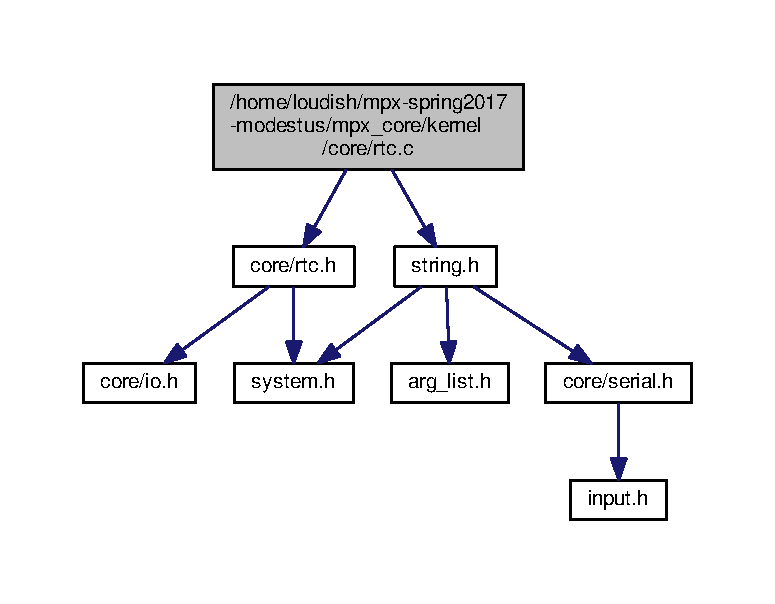
\includegraphics[width=350pt]{rtc_8c__incl}
\end{center}
\end{figure}
\subsection*{Functions}
\begin{DoxyCompactItemize}
\item 
void \hyperlink{rtc_8c_a35fa24488cb7eb077e8dc995729202cf}{get\+\_\+time} (int $\ast$hours, int $\ast$minutes, int $\ast$seconds)
\begin{DoxyCompactList}\small\item\em get\+\_\+time this function will retrieve the system time and place it in three pointers \end{DoxyCompactList}\item 
void \hyperlink{rtc_8c_a9f75815e4f89e0ff7065999f43867e92}{set\+\_\+time} (int hours, int minutes, int seconds)
\begin{DoxyCompactList}\small\item\em set\+\_\+time sets the R\+TC time \end{DoxyCompactList}\item 
void \hyperlink{rtc_8c_ab43f56447c49f42bb4baee3e59e2d1f9}{get\+\_\+date} (int $\ast$day, int $\ast$month, int $\ast$year)
\begin{DoxyCompactList}\small\item\em get\+\_\+date this function will retrieve the system date and place in three pointers \end{DoxyCompactList}\item 
void \hyperlink{rtc_8c_a7903b907981d739e3d156a964255d45e}{set\+\_\+date} (int day, int month, int year)
\begin{DoxyCompactList}\small\item\em set\+\_\+date sets the R\+TC Date \end{DoxyCompactList}\end{DoxyCompactItemize}


\subsection{Function Documentation}
\index{rtc.\+c@{rtc.\+c}!get\+\_\+date@{get\+\_\+date}}
\index{get\+\_\+date@{get\+\_\+date}!rtc.\+c@{rtc.\+c}}
\subsubsection[{\texorpdfstring{get\+\_\+date(int $\ast$day, int $\ast$month, int $\ast$year)}{get_date(int *day, int *month, int *year)}}]{\setlength{\rightskip}{0pt plus 5cm}void get\+\_\+date (
\begin{DoxyParamCaption}
\item[{int $\ast$}]{day, }
\item[{int $\ast$}]{month, }
\item[{int $\ast$}]{year}
\end{DoxyParamCaption}
)}\hypertarget{rtc_8c_ab43f56447c49f42bb4baee3e59e2d1f9}{}\label{rtc_8c_ab43f56447c49f42bb4baee3e59e2d1f9}


get\+\_\+date this function will retrieve the system date and place in three pointers 


\begin{DoxyParams}{Parameters}
{\em day} & pointer to int where the current day will be stored, U\+TC Time zone \\
\hline
{\em months} & pointer to int where the current month will be stored, U\+TC Time zone \\
\hline
{\em year} & pointer to int where the current year will be stored, U\+TC Time zone \\
\hline
\end{DoxyParams}


Definition at line 56 of file rtc.\+c.



References D\+A\+Y\+\_\+\+O\+F\+\_\+\+M\+O\+N\+T\+H\+\_\+\+I\+N\+D\+EX, inb, M\+O\+N\+T\+H\+S\+\_\+\+I\+N\+D\+EX, outb, R\+T\+C\+\_\+\+I\+N\+D\+E\+X\+\_\+\+R\+EG, and Y\+E\+A\+R\+\_\+\+I\+N\+D\+EX.



Referenced by get\+Date(), and kmain().


\begin{DoxyCode}
57 \{
58     \textcolor{keywordtype}{char} temp = 0;
59     \hyperlink{io_8h_a0e661d36f40638a36550a534076f155b}{outb}(\hyperlink{rtc_8h_a52aed4f0dce6c69eec85228a1fc15e2c}{RTC\_INDEX\_REG}, \hyperlink{rtc_8h_a3524da1819943d5a94067c1c9e8aa5cc}{DAY\_OF\_MONTH\_INDEX});
60     temp = \hyperlink{io_8h_ad6488a48837d179b1833e2f48dac9665}{inb}(0x71);
61     *day = ((temp & 0xf0) >>4 ) *10 + (temp & 0x0f);
62 
63     \hyperlink{io_8h_a0e661d36f40638a36550a534076f155b}{outb}(\hyperlink{rtc_8h_a52aed4f0dce6c69eec85228a1fc15e2c}{RTC\_INDEX\_REG}, \hyperlink{rtc_8h_a69a2fa993700fb8058ec48611ebbf5c8}{MONTHS\_INDEX});
64     temp = \hyperlink{io_8h_ad6488a48837d179b1833e2f48dac9665}{inb}(0x71);
65     *month = ((temp & 0xf0) >>4 ) *10 + (temp & 0x0f);
66 
67     \hyperlink{io_8h_a0e661d36f40638a36550a534076f155b}{outb}(\hyperlink{rtc_8h_a52aed4f0dce6c69eec85228a1fc15e2c}{RTC\_INDEX\_REG}, \hyperlink{rtc_8h_a940c790a06a199a1e2136bea0058799e}{YEAR\_INDEX});
68     temp = \hyperlink{io_8h_ad6488a48837d179b1833e2f48dac9665}{inb}(0x71);
69     *year = ((temp & 0xf0) >>4 ) *10 + (temp & 0x0f);
70 \}
\end{DoxyCode}
\index{rtc.\+c@{rtc.\+c}!get\+\_\+time@{get\+\_\+time}}
\index{get\+\_\+time@{get\+\_\+time}!rtc.\+c@{rtc.\+c}}
\subsubsection[{\texorpdfstring{get\+\_\+time(int $\ast$hours, int $\ast$minutes, int $\ast$seconds)}{get_time(int *hours, int *minutes, int *seconds)}}]{\setlength{\rightskip}{0pt plus 5cm}void get\+\_\+time (
\begin{DoxyParamCaption}
\item[{int $\ast$}]{hours, }
\item[{int $\ast$}]{minutes, }
\item[{int $\ast$}]{seconds}
\end{DoxyParamCaption}
)}\hypertarget{rtc_8c_a35fa24488cb7eb077e8dc995729202cf}{}\label{rtc_8c_a35fa24488cb7eb077e8dc995729202cf}


get\+\_\+time this function will retrieve the system time and place it in three pointers 

get\+\_\+time this function will retrieve the system time and place it in three pointers. Military time


\begin{DoxyParams}{Parameters}
{\em hours} & pointer to int where the current hours will be stored, in U\+TC timezone \\
\hline
{\em minutes} & pointer to int where the current minutes will be stored, in U\+TC timezone \\
\hline
{\em seconds} & pointer to int where the current seconds will be stored, in U\+TC timezone \\
\hline
\end{DoxyParams}


Definition at line 10 of file rtc.\+c.



References H\+O\+U\+R\+S\+\_\+\+I\+N\+D\+EX, inb, M\+I\+N\+U\+T\+E\+S\+\_\+\+I\+N\+D\+EX, outb, R\+T\+C\+\_\+\+I\+N\+D\+E\+X\+\_\+\+R\+EG, and S\+E\+C\+O\+N\+D\+S\+\_\+\+I\+N\+D\+EX.



Referenced by get\+Time(), and kmain().


\begin{DoxyCode}
11 \{
12     \textcolor{keywordtype}{char} temp = 0;
13     \hyperlink{io_8h_a0e661d36f40638a36550a534076f155b}{outb}(\hyperlink{rtc_8h_a52aed4f0dce6c69eec85228a1fc15e2c}{RTC\_INDEX\_REG}, \hyperlink{rtc_8h_ad5172920660b0cc3a01124769f769da8}{SECONDS\_INDEX});
14     temp = \hyperlink{io_8h_ad6488a48837d179b1833e2f48dac9665}{inb}(0x71);
15     *seconds = ((temp & 0xf0) >>4 ) *10 + (temp & 0x0f);
16 
17     \hyperlink{io_8h_a0e661d36f40638a36550a534076f155b}{outb}(\hyperlink{rtc_8h_a52aed4f0dce6c69eec85228a1fc15e2c}{RTC\_INDEX\_REG}, \hyperlink{rtc_8h_afb7672d6cea1669acd4f76d74ca28459}{MINUTES\_INDEX});
18     temp = \hyperlink{io_8h_ad6488a48837d179b1833e2f48dac9665}{inb}(0x71);
19     *minutes = ((temp & 0xf0) >>4 ) *10 + (temp & 0x0f);
20 
21     \hyperlink{io_8h_a0e661d36f40638a36550a534076f155b}{outb}(\hyperlink{rtc_8h_a52aed4f0dce6c69eec85228a1fc15e2c}{RTC\_INDEX\_REG}, \hyperlink{rtc_8h_a58095ff2a9d2a6b458d6ef46fa9d4f68}{HOURS\_INDEX});
22     temp = \hyperlink{io_8h_ad6488a48837d179b1833e2f48dac9665}{inb}(0x71);
23     *hours = ((temp & 0xf0) >>4 ) *10 + (temp & 0x0f);
24 \}
\end{DoxyCode}
\index{rtc.\+c@{rtc.\+c}!set\+\_\+date@{set\+\_\+date}}
\index{set\+\_\+date@{set\+\_\+date}!rtc.\+c@{rtc.\+c}}
\subsubsection[{\texorpdfstring{set\+\_\+date(int day, int month, int year)}{set_date(int day, int month, int year)}}]{\setlength{\rightskip}{0pt plus 5cm}void set\+\_\+date (
\begin{DoxyParamCaption}
\item[{int}]{day, }
\item[{int}]{month, }
\item[{int}]{year}
\end{DoxyParamCaption}
)}\hypertarget{rtc_8c_a7903b907981d739e3d156a964255d45e}{}\label{rtc_8c_a7903b907981d739e3d156a964255d45e}


set\+\_\+date sets the R\+TC Date 


\begin{DoxyParams}{Parameters}
{\em day} & the day to set the clock to, must be valid for the month. U\+TC Time zone \\
\hline
{\em month} & the month to set the clock to, must be between 1 and 12. U\+TC Time zone \\
\hline
{\em year} & the year to set the clock to, must be less than 100. U\+TC Time zone \\
\hline
\end{DoxyParams}


Definition at line 79 of file rtc.\+c.



References cli, D\+A\+Y\+\_\+\+O\+F\+\_\+\+M\+O\+N\+T\+H\+\_\+\+I\+N\+D\+EX, M\+O\+N\+T\+H\+S\+\_\+\+I\+N\+D\+EX, outb, R\+T\+C\+\_\+\+D\+A\+T\+A\+\_\+\+R\+EG, R\+T\+C\+\_\+\+I\+N\+D\+E\+X\+\_\+\+R\+EG, sti, and Y\+E\+A\+R\+\_\+\+I\+N\+D\+EX.



Referenced by set\+Date().


\begin{DoxyCode}
80 \{
81     \hyperlink{system_8h_ac5d15f274bc9b1e96230f3d3c60fd1f8}{sti}();
82 
83     \hyperlink{io_8h_a0e661d36f40638a36550a534076f155b}{outb}(\hyperlink{rtc_8h_a52aed4f0dce6c69eec85228a1fc15e2c}{RTC\_INDEX\_REG}, \hyperlink{rtc_8h_a3524da1819943d5a94067c1c9e8aa5cc}{DAY\_OF\_MONTH\_INDEX});
84     \hyperlink{io_8h_a0e661d36f40638a36550a534076f155b}{outb}(\hyperlink{rtc_8h_a2f258a00c59c3f347c8d2d4a75471ce0}{RTC\_DATA\_REG}, ((day/10)<<4)|(day%10));
85 
86     \hyperlink{io_8h_a0e661d36f40638a36550a534076f155b}{outb}(\hyperlink{rtc_8h_a52aed4f0dce6c69eec85228a1fc15e2c}{RTC\_INDEX\_REG}, \hyperlink{rtc_8h_a69a2fa993700fb8058ec48611ebbf5c8}{MONTHS\_INDEX});
87     \hyperlink{io_8h_a0e661d36f40638a36550a534076f155b}{outb}(\hyperlink{rtc_8h_a2f258a00c59c3f347c8d2d4a75471ce0}{RTC\_DATA\_REG}, ((month/10)<<4)|(month%10));
88 
89     \hyperlink{io_8h_a0e661d36f40638a36550a534076f155b}{outb}(\hyperlink{rtc_8h_a52aed4f0dce6c69eec85228a1fc15e2c}{RTC\_INDEX\_REG}, \hyperlink{rtc_8h_a940c790a06a199a1e2136bea0058799e}{YEAR\_INDEX});
90     \hyperlink{io_8h_a0e661d36f40638a36550a534076f155b}{outb}(\hyperlink{rtc_8h_a2f258a00c59c3f347c8d2d4a75471ce0}{RTC\_DATA\_REG}, (((year-(year/100)*100)/10)<<4)|(year%10) );
91 
92     \hyperlink{system_8h_a68c330e94fe121eba993e5a5973c3162}{cli}();
93 \}
\end{DoxyCode}
\index{rtc.\+c@{rtc.\+c}!set\+\_\+time@{set\+\_\+time}}
\index{set\+\_\+time@{set\+\_\+time}!rtc.\+c@{rtc.\+c}}
\subsubsection[{\texorpdfstring{set\+\_\+time(int hours, int minutes, int seconds)}{set_time(int hours, int minutes, int seconds)}}]{\setlength{\rightskip}{0pt plus 5cm}void set\+\_\+time (
\begin{DoxyParamCaption}
\item[{int}]{hours, }
\item[{int}]{minutes, }
\item[{int}]{seconds}
\end{DoxyParamCaption}
)}\hypertarget{rtc_8c_a9f75815e4f89e0ff7065999f43867e92}{}\label{rtc_8c_a9f75815e4f89e0ff7065999f43867e92}


set\+\_\+time sets the R\+TC time 

set\+\_\+time sets the R\+TC time. Military time


\begin{DoxyParams}{Parameters}
{\em hours} & the hours to set the clock to, must be less than 24. In U\+TC Time zone \\
\hline
{\em minutes} & the minutes to set the clock to, must be less than 60. In U\+TC Time zone \\
\hline
{\em seconds} & the seconds to set the clock to, must be less than 60. In U\+TC Time zone \\
\hline
\end{DoxyParams}


Definition at line 33 of file rtc.\+c.



References cli, H\+O\+U\+R\+S\+\_\+\+I\+N\+D\+EX, M\+I\+N\+U\+T\+E\+S\+\_\+\+I\+N\+D\+EX, outb, R\+T\+C\+\_\+\+D\+A\+T\+A\+\_\+\+R\+EG, R\+T\+C\+\_\+\+I\+N\+D\+E\+X\+\_\+\+R\+EG, S\+E\+C\+O\+N\+D\+S\+\_\+\+I\+N\+D\+EX, and sti.



Referenced by set\+Time().


\begin{DoxyCode}
34 \{
35     \hyperlink{system_8h_ac5d15f274bc9b1e96230f3d3c60fd1f8}{sti}();
36 
37     \hyperlink{io_8h_a0e661d36f40638a36550a534076f155b}{outb}(\hyperlink{rtc_8h_a52aed4f0dce6c69eec85228a1fc15e2c}{RTC\_INDEX\_REG}, \hyperlink{rtc_8h_a58095ff2a9d2a6b458d6ef46fa9d4f68}{HOURS\_INDEX});
38     \hyperlink{io_8h_a0e661d36f40638a36550a534076f155b}{outb}(\hyperlink{rtc_8h_a2f258a00c59c3f347c8d2d4a75471ce0}{RTC\_DATA\_REG}, ((hours/10)<<4)|(hours%10) );
39 
40     \hyperlink{io_8h_a0e661d36f40638a36550a534076f155b}{outb}(\hyperlink{rtc_8h_a52aed4f0dce6c69eec85228a1fc15e2c}{RTC\_INDEX\_REG}, \hyperlink{rtc_8h_afb7672d6cea1669acd4f76d74ca28459}{MINUTES\_INDEX});
41     \hyperlink{io_8h_a0e661d36f40638a36550a534076f155b}{outb}(\hyperlink{rtc_8h_a2f258a00c59c3f347c8d2d4a75471ce0}{RTC\_DATA\_REG}, ((minutes/10)<<4)|(minutes%10) );
42 
43     \hyperlink{io_8h_a0e661d36f40638a36550a534076f155b}{outb}(\hyperlink{rtc_8h_a52aed4f0dce6c69eec85228a1fc15e2c}{RTC\_INDEX\_REG}, \hyperlink{rtc_8h_ad5172920660b0cc3a01124769f769da8}{SECONDS\_INDEX});
44     \hyperlink{io_8h_a0e661d36f40638a36550a534076f155b}{outb}(\hyperlink{rtc_8h_a2f258a00c59c3f347c8d2d4a75471ce0}{RTC\_DATA\_REG}, ((seconds/10)<<4)|(seconds%10) );
45 
46     \hyperlink{system_8h_a68c330e94fe121eba993e5a5973c3162}{cli}();
47 \}
\end{DoxyCode}

\hypertarget{serial_8c}{}\section{/home/loudish/mpx-\/spring2017-\/modestus/mpx\+\_\+core/kernel/core/serial.c File Reference}
\label{serial_8c}\index{/home/loudish/mpx-\/spring2017-\/modestus/mpx\+\_\+core/kernel/core/serial.\+c@{/home/loudish/mpx-\/spring2017-\/modestus/mpx\+\_\+core/kernel/core/serial.\+c}}
{\ttfamily \#include $<$stdint.\+h$>$}\\*
{\ttfamily \#include $<$string.\+h$>$}\\*
{\ttfamily \#include $<$core/io.\+h$>$}\\*
{\ttfamily \#include $<$core/serial.\+h$>$}\\*
{\ttfamily \#include $<$core/commhand.\+h$>$}\\*
{\ttfamily \#include $<$input.\+h$>$}\\*
Include dependency graph for serial.\+c\+:\nopagebreak
\begin{figure}[H]
\begin{center}
\leavevmode
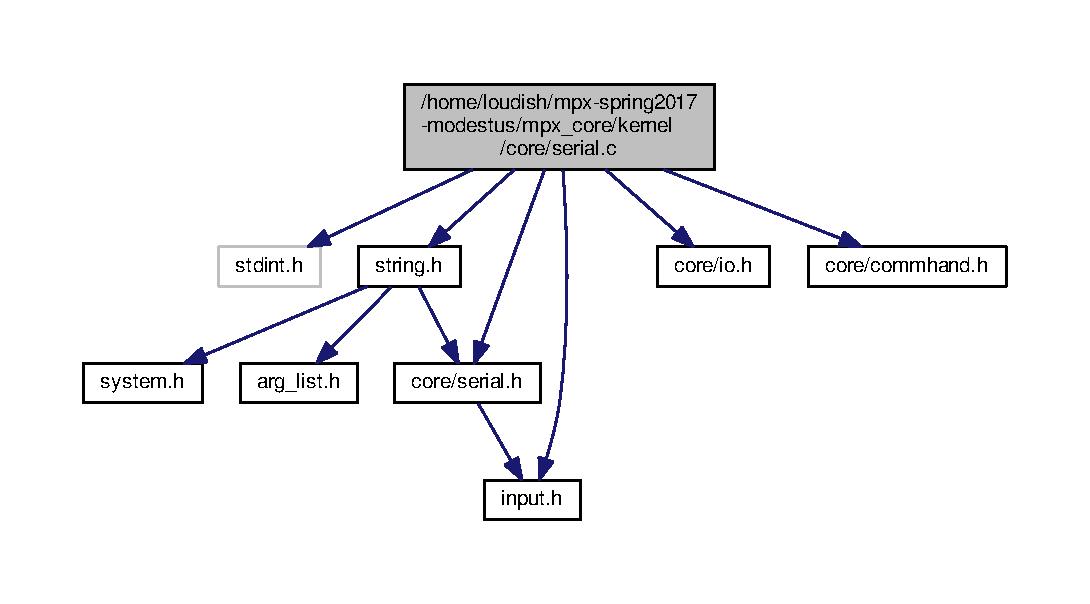
\includegraphics[width=350pt]{serial_8c__incl}
\end{center}
\end{figure}
\subsection*{Macros}
\begin{DoxyCompactItemize}
\item 
\#define \hyperlink{serial_8c_a258bb72419ef143530a2f8f55e7d57af}{N\+O\+\_\+\+E\+R\+R\+OR}~0
\end{DoxyCompactItemize}
\subsection*{Functions}
\begin{DoxyCompactItemize}
\item 
int \hyperlink{serial_8c_a7078c07ff8b2c48780558549a8f7cf90}{init\+\_\+serial} (int device)
\item 
int \hyperlink{serial_8c_a3514f7abff236a4e00a6c46021ce5e22}{serial\+\_\+println} (const char $\ast$msg)
\item 
int \hyperlink{serial_8c_a995827efcd4dcfb780c9fbb9645410a4}{serial\+\_\+print} (const char $\ast$msg)
\item 
int \hyperlink{serial_8c_ae97b87ee1f57c687e7fca6f9958e03ef}{set\+\_\+serial\+\_\+out} (int device)
\item 
int \hyperlink{serial_8c_a3f4008da5feabfb7e086f6673a81104b}{set\+\_\+serial\+\_\+in} (int device)
\item 
void \hyperlink{serial_8c_a337da5154672f3b359cf70d7b78f0c0d}{clear\+\_\+buff} ()
\item 
void \hyperlink{serial_8c_a8f0293a95ba79d7dafe198c2cb75549f}{return\+\_\+cursor} (int cursor\+\_\+loc, int length)
\item 
char $\ast$ \hyperlink{serial_8c_a4b7cdfe478986c0d41a54f2c4a683136}{serial\+\_\+poll} (char \hyperlink{commhand_8c_a304f731e770f19e932c39d189c8cb56f}{in\+\_\+string}\mbox{[}\hyperlink{input_8h_a7a9a231e30b47bc0345749c8bd1e5077}{M\+A\+X\+\_\+\+L\+E\+N\+G\+TH}\mbox{]})
\end{DoxyCompactItemize}
\subsection*{Variables}
\begin{DoxyCompactItemize}
\item 
int \hyperlink{serial_8c_adbb2c18b0aaab5c1927a6f674768a710}{serial\+\_\+port\+\_\+out} = 0
\item 
int \hyperlink{serial_8c_a1a756238531fc5bf1096f89dc18e835e}{serial\+\_\+port\+\_\+in} = 0
\end{DoxyCompactItemize}


\subsection{Macro Definition Documentation}
\index{serial.\+c@{serial.\+c}!N\+O\+\_\+\+E\+R\+R\+OR@{N\+O\+\_\+\+E\+R\+R\+OR}}
\index{N\+O\+\_\+\+E\+R\+R\+OR@{N\+O\+\_\+\+E\+R\+R\+OR}!serial.\+c@{serial.\+c}}
\subsubsection[{\texorpdfstring{N\+O\+\_\+\+E\+R\+R\+OR}{NO_ERROR}}]{\setlength{\rightskip}{0pt plus 5cm}\#define N\+O\+\_\+\+E\+R\+R\+OR~0}\hypertarget{serial_8c_a258bb72419ef143530a2f8f55e7d57af}{}\label{serial_8c_a258bb72419ef143530a2f8f55e7d57af}


Definition at line 16 of file serial.\+c.



Referenced by init\+\_\+serial(), serial\+\_\+print(), serial\+\_\+println(), set\+\_\+serial\+\_\+in(), and set\+\_\+serial\+\_\+out().



\subsection{Function Documentation}
\index{serial.\+c@{serial.\+c}!clear\+\_\+buff@{clear\+\_\+buff}}
\index{clear\+\_\+buff@{clear\+\_\+buff}!serial.\+c@{serial.\+c}}
\subsubsection[{\texorpdfstring{clear\+\_\+buff()}{clear_buff()}}]{\setlength{\rightskip}{0pt plus 5cm}void clear\+\_\+buff (
\begin{DoxyParamCaption}
{}
\end{DoxyParamCaption}
)}\hypertarget{serial_8c_a337da5154672f3b359cf70d7b78f0c0d}{}\label{serial_8c_a337da5154672f3b359cf70d7b78f0c0d}


Definition at line 94 of file serial.\+c.



References serial\+\_\+print().



Referenced by serial\+\_\+poll().


\begin{DoxyCode}
94                   \{
95     \hyperlink{serial_8c_a995827efcd4dcfb780c9fbb9645410a4}{serial\_print}(\textcolor{stringliteral}{"\(\backslash\)033[2K"});
96     \hyperlink{serial_8c_a995827efcd4dcfb780c9fbb9645410a4}{serial\_print}(\textcolor{stringliteral}{"\(\backslash\)033[G"});
97     \hyperlink{serial_8c_a995827efcd4dcfb780c9fbb9645410a4}{serial\_print}(\textcolor{stringliteral}{"> "});
98 \}
\end{DoxyCode}
\index{serial.\+c@{serial.\+c}!init\+\_\+serial@{init\+\_\+serial}}
\index{init\+\_\+serial@{init\+\_\+serial}!serial.\+c@{serial.\+c}}
\subsubsection[{\texorpdfstring{init\+\_\+serial(int device)}{init_serial(int device)}}]{\setlength{\rightskip}{0pt plus 5cm}int init\+\_\+serial (
\begin{DoxyParamCaption}
\item[{int}]{device}
\end{DoxyParamCaption}
)}\hypertarget{serial_8c_a7078c07ff8b2c48780558549a8f7cf90}{}\label{serial_8c_a7078c07ff8b2c48780558549a8f7cf90}


Definition at line 26 of file serial.\+c.



References inb, N\+O\+\_\+\+E\+R\+R\+OR, and outb.


\begin{DoxyCode}
27 \{
28   \hyperlink{io_8h_a0e661d36f40638a36550a534076f155b}{outb}(device + 1, 0x00); \textcolor{comment}{//disable interrupts}
29   \hyperlink{io_8h_a0e661d36f40638a36550a534076f155b}{outb}(device + 3, 0x80); \textcolor{comment}{//set line control register}
30   \hyperlink{io_8h_a0e661d36f40638a36550a534076f155b}{outb}(device + 0, 115200/9600); \textcolor{comment}{//set bsd least sig bit}
31   \hyperlink{io_8h_a0e661d36f40638a36550a534076f155b}{outb}(device + 1, 0x00); \textcolor{comment}{//brd most significant bit}
32   \hyperlink{io_8h_a0e661d36f40638a36550a534076f155b}{outb}(device + 3, 0x03); \textcolor{comment}{//lock divisor; 8bits, no parity, one stop}
33   \hyperlink{io_8h_a0e661d36f40638a36550a534076f155b}{outb}(device + 2, 0xC7); \textcolor{comment}{//enable fifo, clear, 14byte threshold}
34   \hyperlink{io_8h_a0e661d36f40638a36550a534076f155b}{outb}(device + 4, 0x0B); \textcolor{comment}{//enable interrupts, rts/dsr set}
35   (void)\hyperlink{io_8h_ad6488a48837d179b1833e2f48dac9665}{inb}(device);      \textcolor{comment}{//read bit to reset port}
36   \textcolor{keywordflow}{return} \hyperlink{serial_8c_a258bb72419ef143530a2f8f55e7d57af}{NO\_ERROR};
37 \}
\end{DoxyCode}
\index{serial.\+c@{serial.\+c}!return\+\_\+cursor@{return\+\_\+cursor}}
\index{return\+\_\+cursor@{return\+\_\+cursor}!serial.\+c@{serial.\+c}}
\subsubsection[{\texorpdfstring{return\+\_\+cursor(int cursor\+\_\+loc, int length)}{return_cursor(int cursor_loc, int length)}}]{\setlength{\rightskip}{0pt plus 5cm}void return\+\_\+cursor (
\begin{DoxyParamCaption}
\item[{int}]{cursor\+\_\+loc, }
\item[{int}]{length}
\end{DoxyParamCaption}
)}\hypertarget{serial_8c_a8f0293a95ba79d7dafe198c2cb75549f}{}\label{serial_8c_a8f0293a95ba79d7dafe198c2cb75549f}


Definition at line 100 of file serial.\+c.



References serial\+\_\+print().



Referenced by serial\+\_\+poll().


\begin{DoxyCode}
100                                                \{
101     \textcolor{keywordtype}{int} move = length - cursor\_loc;
102     \textcolor{keywordtype}{int} i = 0;
103     \textcolor{keywordflow}{for} (; i < move; i++) \{
104         \hyperlink{serial_8c_a995827efcd4dcfb780c9fbb9645410a4}{serial\_print}(\textcolor{stringliteral}{"\(\backslash\)033[D"});
105     \}
106 \}
\end{DoxyCode}
\index{serial.\+c@{serial.\+c}!serial\+\_\+poll@{serial\+\_\+poll}}
\index{serial\+\_\+poll@{serial\+\_\+poll}!serial.\+c@{serial.\+c}}
\subsubsection[{\texorpdfstring{serial\+\_\+poll(char in\+\_\+string[M\+A\+X\+\_\+\+L\+E\+N\+G\+TH])}{serial_poll(char in_string[MAX_LENGTH])}}]{\setlength{\rightskip}{0pt plus 5cm}char$\ast$ serial\+\_\+poll (
\begin{DoxyParamCaption}
\item[{char}]{in\+\_\+string\mbox{[}\+M\+A\+X\+\_\+\+L\+E\+N\+G\+T\+H\mbox{]}}
\end{DoxyParamCaption}
)}\hypertarget{serial_8c_a4b7cdfe478986c0d41a54f2c4a683136}{}\label{serial_8c_a4b7cdfe478986c0d41a54f2c4a683136}


Definition at line 114 of file serial.\+c.



References B\+A\+C\+K\+S\+P\+A\+CE, clear\+\_\+buff(), C\+O\+M1, D\+E\+L\+E\+TE, E\+SC, in\+\_\+string, inb, N\+E\+W\+\_\+\+L\+I\+NE, R\+E\+T\+U\+RN, return\+\_\+cursor(), serial\+\_\+print(), and strcpy().



Referenced by init\+\_\+commhand().


\begin{DoxyCode}
114                                               \{
115     \textcolor{comment}{//in\_char is the character read from the register}
116     \textcolor{comment}{//out\_char is that character with a null terminator appended on the end}
117     \textcolor{comment}{//length is the current size of the input}
118     \textcolor{comment}{//cursor\_loc is the current location of the cursor in the input}
119     \textcolor{keywordtype}{char} in\_char;
120     \textcolor{keywordtype}{char} out\_char[2];
121     out\_char[1] = \textcolor{charliteral}{'\(\backslash\)0'};
122     \textcolor{keywordtype}{int} length = 0;
123     \textcolor{keywordtype}{int} cursor\_loc = 0;
124 
125     \textcolor{comment}{//polling for user input}
126     \textcolor{keywordflow}{while} (1) \{
127 
128         \textcolor{keywordflow}{if} (\hyperlink{io_8h_ad6488a48837d179b1833e2f48dac9665}{inb}(\hyperlink{serial_8h_a00dbb3ab1c59e14699be9393693e2248}{COM1}+5)&1) \{
129             \textcolor{comment}{//the character is read from the register}
130             in\_char = \hyperlink{io_8h_ad6488a48837d179b1833e2f48dac9665}{inb}(\hyperlink{serial_8h_a00dbb3ab1c59e14699be9393693e2248}{COM1});
131             out\_char[0] = in\_char;
132 
133             \textcolor{keywordflow}{if} (in\_char == \hyperlink{input_8h_a629568514359445d2fbda71d70eeb1ce}{BACKSPACE}) \{
134                 \textcolor{keywordflow}{if} (length != 0) \{
135                     \textcolor{keywordflow}{if} (cursor\_loc == length)
136                     \{
137                         cursor\_loc--;
138                         \hyperlink{commhand_8c_a304f731e770f19e932c39d189c8cb56f}{in\_string}[cursor\_loc] = \textcolor{charliteral}{'\(\backslash\)0'};
139                         \hyperlink{serial_8c_a337da5154672f3b359cf70d7b78f0c0d}{clear\_buff}();
140                         \hyperlink{serial_8c_a995827efcd4dcfb780c9fbb9645410a4}{serial\_print}(\hyperlink{commhand_8c_a304f731e770f19e932c39d189c8cb56f}{in\_string});
141                         length--;
142                         \hyperlink{serial_8c_a8f0293a95ba79d7dafe198c2cb75549f}{return\_cursor}(cursor\_loc, length);
143 
144                     \}
145                     \textcolor{keywordflow}{else}
146                     \{
147                         cursor\_loc--;
148                         \hyperlink{string_8h_a1eb9cae61e6a6282c28dbc298ef7297e}{strcpy}(&\hyperlink{commhand_8c_a304f731e770f19e932c39d189c8cb56f}{in\_string}[cursor\_loc], &\hyperlink{commhand_8c_a304f731e770f19e932c39d189c8cb56f}{in\_string}[cursor\_loc + 1]);
149                         \hyperlink{commhand_8c_a304f731e770f19e932c39d189c8cb56f}{in\_string}[length - 1] = \textcolor{charliteral}{'\(\backslash\)0'};
150                         \hyperlink{serial_8c_a337da5154672f3b359cf70d7b78f0c0d}{clear\_buff}();
151                         \hyperlink{serial_8c_a995827efcd4dcfb780c9fbb9645410a4}{serial\_print}(\hyperlink{commhand_8c_a304f731e770f19e932c39d189c8cb56f}{in\_string});
152                         length--;
153                         \hyperlink{serial_8c_a8f0293a95ba79d7dafe198c2cb75549f}{return\_cursor}(cursor\_loc, length);
154                     \}
155                 \}
156             \} \textcolor{keywordflow}{else} \textcolor{keywordflow}{if} (in\_char == \hyperlink{input_8h_abbbe5949f3c1f72e439924f8cf503509}{DELETE}) \{
157             \} \textcolor{keywordflow}{else} \textcolor{keywordflow}{if} (in\_char == \hyperlink{input_8h_a6a0e6b80dd3d5ca395cf58151749f5e2}{RETURN} || in\_char == \hyperlink{input_8h_a7b99dc1e1c86b4897498c2d436ead1b5}{NEW\_LINE}) \{
158                     
159                 \textcolor{keywordflow}{return} \hyperlink{commhand_8c_a304f731e770f19e932c39d189c8cb56f}{in\_string};
160             \} \textcolor{keywordflow}{else} \textcolor{keywordflow}{if} (in\_char == \hyperlink{input_8h_a4af1b6159e447ba72652bb7fcdfa726e}{ESC}) \{
161                 \textcolor{comment}{//buffer through ansi escape keys ([)}
162                 in\_char = \hyperlink{io_8h_ad6488a48837d179b1833e2f48dac9665}{inb}(\hyperlink{serial_8h_a00dbb3ab1c59e14699be9393693e2248}{COM1});
163                 in\_char = \hyperlink{io_8h_ad6488a48837d179b1833e2f48dac9665}{inb}(\hyperlink{serial_8h_a00dbb3ab1c59e14699be9393693e2248}{COM1});
164 
165                 \textcolor{keywordflow}{if} (in\_char == \textcolor{charliteral}{'A'}) \{           \textcolor{comment}{//UP}
166                     \hyperlink{serial_8c_a337da5154672f3b359cf70d7b78f0c0d}{clear\_buff}();
167                     \hyperlink{commhand_8c_a304f731e770f19e932c39d189c8cb56f}{in\_string}[0] = \textcolor{charliteral}{'\(\backslash\)0'};
168                     cursor\_loc = 0;
169                     length = 0;
170                     \textcolor{comment}{//go backwards in command history}
171                 \} \textcolor{keywordflow}{else} \textcolor{keywordflow}{if} (in\_char == \textcolor{charliteral}{'B'}) \{    \textcolor{comment}{//DOWN}
172                     \hyperlink{serial_8c_a337da5154672f3b359cf70d7b78f0c0d}{clear\_buff}();
173                     \hyperlink{commhand_8c_a304f731e770f19e932c39d189c8cb56f}{in\_string}[0] = \textcolor{charliteral}{'\(\backslash\)0'};
174                     cursor\_loc = 0;
175                     length = 0;
176                     \textcolor{comment}{//go forward in command history}
177                 \} \textcolor{keywordflow}{else} \textcolor{keywordflow}{if} (in\_char == \textcolor{charliteral}{'C'}) \{    \textcolor{comment}{//RIGHT}
178                     \textcolor{keywordflow}{if} (cursor\_loc < length) \{
179                         \hyperlink{serial_8c_a995827efcd4dcfb780c9fbb9645410a4}{serial\_print}(\textcolor{stringliteral}{"\(\backslash\)033[C"}); 
180                         cursor\_loc++;
181                     \}
182                 \} \textcolor{keywordflow}{else} \textcolor{keywordflow}{if} (in\_char == \textcolor{charliteral}{'D'}) \{    \textcolor{comment}{//LEFT}
183                     \textcolor{keywordflow}{if} (cursor\_loc > 0) \{
184                         \hyperlink{serial_8c_a995827efcd4dcfb780c9fbb9645410a4}{serial\_print}(\textcolor{stringliteral}{"\(\backslash\)033[D"});
185                         cursor\_loc--;
186                     \}   
187                 \} \textcolor{keywordflow}{else} \textcolor{keywordflow}{if} (in\_char == \textcolor{charliteral}{'3'}) \{  \textcolor{comment}{//DEL}
188                     \hyperlink{string_8h_a1eb9cae61e6a6282c28dbc298ef7297e}{strcpy}(&\hyperlink{commhand_8c_a304f731e770f19e932c39d189c8cb56f}{in\_string}[cursor\_loc], &\hyperlink{commhand_8c_a304f731e770f19e932c39d189c8cb56f}{in\_string}[cursor\_loc + 1]);
189                     \hyperlink{commhand_8c_a304f731e770f19e932c39d189c8cb56f}{in\_string}[length] = \textcolor{charliteral}{'\(\backslash\)0'};
190                     \hyperlink{serial_8c_a337da5154672f3b359cf70d7b78f0c0d}{clear\_buff}();
191                     \hyperlink{serial_8c_a995827efcd4dcfb780c9fbb9645410a4}{serial\_print}(\hyperlink{commhand_8c_a304f731e770f19e932c39d189c8cb56f}{in\_string});
192                     length--;
193                     \hyperlink{serial_8c_a8f0293a95ba79d7dafe198c2cb75549f}{return\_cursor}(cursor\_loc, length);
194                 \}
195 
196             \} \textcolor{keywordflow}{else} \{
197                 \textcolor{keywordflow}{if} (length < \hyperlink{input_8h_a7a9a231e30b47bc0345749c8bd1e5077}{MAX\_LENGTH} - 1) \{
198                     \textcolor{keywordflow}{if} (length == cursor\_loc) \{
199                         \hyperlink{commhand_8c_a304f731e770f19e932c39d189c8cb56f}{in\_string}[length] = in\_char;
200                         \hyperlink{commhand_8c_a304f731e770f19e932c39d189c8cb56f}{in\_string}[length + 1] = \textcolor{charliteral}{'\(\backslash\)0'};
201                         \hyperlink{serial_8c_a995827efcd4dcfb780c9fbb9645410a4}{serial\_print}(out\_char);
202                         cursor\_loc++;
203                         length++;
204                     \}
205                     \textcolor{keywordflow}{else} \{
206                         \textcolor{keywordtype}{int} i = length;
207                         \hyperlink{commhand_8c_a304f731e770f19e932c39d189c8cb56f}{in\_string}[length+1] = \textcolor{charliteral}{'\(\backslash\)0'};
208                         \textcolor{keywordflow}{for} (; i >= cursor\_loc; i--) \{
209                             \hyperlink{commhand_8c_a304f731e770f19e932c39d189c8cb56f}{in\_string}[i + 1] = \hyperlink{commhand_8c_a304f731e770f19e932c39d189c8cb56f}{in\_string}[i]; 
210                         \}
211                         \hyperlink{commhand_8c_a304f731e770f19e932c39d189c8cb56f}{in\_string}[cursor\_loc] = in\_char;
212                         length++;
213                         cursor\_loc++;
214                         \hyperlink{serial_8c_a337da5154672f3b359cf70d7b78f0c0d}{clear\_buff}();
215                         \hyperlink{serial_8c_a995827efcd4dcfb780c9fbb9645410a4}{serial\_print}(\hyperlink{commhand_8c_a304f731e770f19e932c39d189c8cb56f}{in\_string});
216                         \hyperlink{serial_8c_a8f0293a95ba79d7dafe198c2cb75549f}{return\_cursor}(cursor\_loc, length);
217                     \}
218                 \}
219             \}
220         \}
221     \}
222     \textcolor{keywordflow}{return} \hyperlink{commhand_8c_a304f731e770f19e932c39d189c8cb56f}{in\_string};
223 \}
\end{DoxyCode}
\index{serial.\+c@{serial.\+c}!serial\+\_\+print@{serial\+\_\+print}}
\index{serial\+\_\+print@{serial\+\_\+print}!serial.\+c@{serial.\+c}}
\subsubsection[{\texorpdfstring{serial\+\_\+print(const char $\ast$msg)}{serial_print(const char *msg)}}]{\setlength{\rightskip}{0pt plus 5cm}int serial\+\_\+print (
\begin{DoxyParamCaption}
\item[{const char $\ast$}]{msg}
\end{DoxyParamCaption}
)}\hypertarget{serial_8c_a995827efcd4dcfb780c9fbb9645410a4}{}\label{serial_8c_a995827efcd4dcfb780c9fbb9645410a4}


Definition at line 59 of file serial.\+c.



References N\+O\+\_\+\+E\+R\+R\+OR, outb, and serial\+\_\+port\+\_\+out.



Referenced by clear\+\_\+buff(), do\+\_\+isr(), get\+Time(), init\+\_\+commhand(), pcb\+Func(), return\+\_\+cursor(), serial\+\_\+poll(), and version().


\begin{DoxyCode}
60 \{
61   \textcolor{keywordtype}{int} i;
62   \textcolor{keywordflow}{for}(i=0; *(i+msg)!=\textcolor{charliteral}{'\(\backslash\)0'}; i++)\{
63     \hyperlink{io_8h_a0e661d36f40638a36550a534076f155b}{outb}(\hyperlink{serial_8c_adbb2c18b0aaab5c1927a6f674768a710}{serial\_port\_out},*(i+msg));
64   \}
65   \textcolor{keywordflow}{if} (*msg == \textcolor{charliteral}{'\(\backslash\)r'}) \hyperlink{io_8h_a0e661d36f40638a36550a534076f155b}{outb}(\hyperlink{serial_8c_adbb2c18b0aaab5c1927a6f674768a710}{serial\_port\_out},\textcolor{charliteral}{'\(\backslash\)n'});
66   \textcolor{keywordflow}{return} \hyperlink{serial_8c_a258bb72419ef143530a2f8f55e7d57af}{NO\_ERROR};
67 \}
\end{DoxyCode}
\index{serial.\+c@{serial.\+c}!serial\+\_\+println@{serial\+\_\+println}}
\index{serial\+\_\+println@{serial\+\_\+println}!serial.\+c@{serial.\+c}}
\subsubsection[{\texorpdfstring{serial\+\_\+println(const char $\ast$msg)}{serial_println(const char *msg)}}]{\setlength{\rightskip}{0pt plus 5cm}int serial\+\_\+println (
\begin{DoxyParamCaption}
\item[{const char $\ast$}]{msg}
\end{DoxyParamCaption}
)}\hypertarget{serial_8c_a3514f7abff236a4e00a6c46021ce5e22}{}\label{serial_8c_a3514f7abff236a4e00a6c46021ce5e22}


Definition at line 44 of file serial.\+c.



References N\+O\+\_\+\+E\+R\+R\+OR, outb, and serial\+\_\+port\+\_\+out.



Referenced by alloc(), clear\+\_\+screen(), date(), do\+\_\+isr(), do\+\_\+reserved(), exec\+\_\+comm(), help(), help\+Create\+P\+C\+B(), help\+Date(), help\+Func(), help\+Get\+Date(), help\+Get\+Time(), help\+Get\+Version(), help\+Resume\+P\+C\+B(), help\+Set\+Date(), help\+Set\+Priority(), help\+Set\+Time(), help\+Show\+All\+Processes(), help\+Show\+Blocked\+Processes(), help\+Show\+P\+C\+B(), help\+Show\+Ready\+Processes(), help\+Shutdown(), help\+Suspend\+P\+C\+B(), help\+Time(), help\+Version(), klogv(), pcb\+Func(), set\+Date(), set\+Time(), shutdown\+Func(), start\+\_\+up\+\_\+anim(), time(), and version().


\begin{DoxyCode}
45 \{
46   \textcolor{keywordtype}{int} i;
47   \textcolor{keywordflow}{for}(i=0; *(i+msg)!=\textcolor{charliteral}{'\(\backslash\)0'}; i++)\{
48     \hyperlink{io_8h_a0e661d36f40638a36550a534076f155b}{outb}(\hyperlink{serial_8c_adbb2c18b0aaab5c1927a6f674768a710}{serial\_port\_out},*(i+msg));
49   \}
50   \hyperlink{io_8h_a0e661d36f40638a36550a534076f155b}{outb}(\hyperlink{serial_8c_adbb2c18b0aaab5c1927a6f674768a710}{serial\_port\_out},\textcolor{charliteral}{'\(\backslash\)r'});
51   \hyperlink{io_8h_a0e661d36f40638a36550a534076f155b}{outb}(\hyperlink{serial_8c_adbb2c18b0aaab5c1927a6f674768a710}{serial\_port\_out},\textcolor{charliteral}{'\(\backslash\)n'});  
52   \textcolor{keywordflow}{return} \hyperlink{serial_8c_a258bb72419ef143530a2f8f55e7d57af}{NO\_ERROR};
53 \}
\end{DoxyCode}
\index{serial.\+c@{serial.\+c}!set\+\_\+serial\+\_\+in@{set\+\_\+serial\+\_\+in}}
\index{set\+\_\+serial\+\_\+in@{set\+\_\+serial\+\_\+in}!serial.\+c@{serial.\+c}}
\subsubsection[{\texorpdfstring{set\+\_\+serial\+\_\+in(int device)}{set_serial_in(int device)}}]{\setlength{\rightskip}{0pt plus 5cm}int set\+\_\+serial\+\_\+in (
\begin{DoxyParamCaption}
\item[{int}]{device}
\end{DoxyParamCaption}
)}\hypertarget{serial_8c_a3f4008da5feabfb7e086f6673a81104b}{}\label{serial_8c_a3f4008da5feabfb7e086f6673a81104b}


Definition at line 87 of file serial.\+c.



References N\+O\+\_\+\+E\+R\+R\+OR, and serial\+\_\+port\+\_\+in.



Referenced by kmain().


\begin{DoxyCode}
88 \{
89   \hyperlink{serial_8c_a1a756238531fc5bf1096f89dc18e835e}{serial\_port\_in} = device;
90   \textcolor{keywordflow}{return} \hyperlink{serial_8c_a258bb72419ef143530a2f8f55e7d57af}{NO\_ERROR};
91 \}
\end{DoxyCode}
\index{serial.\+c@{serial.\+c}!set\+\_\+serial\+\_\+out@{set\+\_\+serial\+\_\+out}}
\index{set\+\_\+serial\+\_\+out@{set\+\_\+serial\+\_\+out}!serial.\+c@{serial.\+c}}
\subsubsection[{\texorpdfstring{set\+\_\+serial\+\_\+out(int device)}{set_serial_out(int device)}}]{\setlength{\rightskip}{0pt plus 5cm}int set\+\_\+serial\+\_\+out (
\begin{DoxyParamCaption}
\item[{int}]{device}
\end{DoxyParamCaption}
)}\hypertarget{serial_8c_ae97b87ee1f57c687e7fca6f9958e03ef}{}\label{serial_8c_ae97b87ee1f57c687e7fca6f9958e03ef}


Definition at line 75 of file serial.\+c.



References N\+O\+\_\+\+E\+R\+R\+OR, and serial\+\_\+port\+\_\+out.



Referenced by kmain().


\begin{DoxyCode}
76 \{
77   \hyperlink{serial_8c_adbb2c18b0aaab5c1927a6f674768a710}{serial\_port\_out} = device;
78   \textcolor{keywordflow}{return} \hyperlink{serial_8c_a258bb72419ef143530a2f8f55e7d57af}{NO\_ERROR};
79 \}
\end{DoxyCode}


\subsection{Variable Documentation}
\index{serial.\+c@{serial.\+c}!serial\+\_\+port\+\_\+in@{serial\+\_\+port\+\_\+in}}
\index{serial\+\_\+port\+\_\+in@{serial\+\_\+port\+\_\+in}!serial.\+c@{serial.\+c}}
\subsubsection[{\texorpdfstring{serial\+\_\+port\+\_\+in}{serial_port_in}}]{\setlength{\rightskip}{0pt plus 5cm}int serial\+\_\+port\+\_\+in = 0}\hypertarget{serial_8c_a1a756238531fc5bf1096f89dc18e835e}{}\label{serial_8c_a1a756238531fc5bf1096f89dc18e835e}


Definition at line 20 of file serial.\+c.



Referenced by set\+\_\+serial\+\_\+in().

\index{serial.\+c@{serial.\+c}!serial\+\_\+port\+\_\+out@{serial\+\_\+port\+\_\+out}}
\index{serial\+\_\+port\+\_\+out@{serial\+\_\+port\+\_\+out}!serial.\+c@{serial.\+c}}
\subsubsection[{\texorpdfstring{serial\+\_\+port\+\_\+out}{serial_port_out}}]{\setlength{\rightskip}{0pt plus 5cm}int serial\+\_\+port\+\_\+out = 0}\hypertarget{serial_8c_adbb2c18b0aaab5c1927a6f674768a710}{}\label{serial_8c_adbb2c18b0aaab5c1927a6f674768a710}


Definition at line 19 of file serial.\+c.



Referenced by serial\+\_\+print(), serial\+\_\+println(), and set\+\_\+serial\+\_\+out().


\hypertarget{system_8c}{}\section{/home/loudish/mpx-\/spring2017-\/modestus/mpx\+\_\+core/kernel/core/system.c File Reference}
\label{system_8c}\index{/home/loudish/mpx-\/spring2017-\/modestus/mpx\+\_\+core/kernel/core/system.\+c@{/home/loudish/mpx-\/spring2017-\/modestus/mpx\+\_\+core/kernel/core/system.\+c}}
{\ttfamily \#include $<$string.\+h$>$}\\*
{\ttfamily \#include $<$system.\+h$>$}\\*
{\ttfamily \#include $<$core/serial.\+h$>$}\\*
Include dependency graph for system.\+c\+:\nopagebreak
\begin{figure}[H]
\begin{center}
\leavevmode
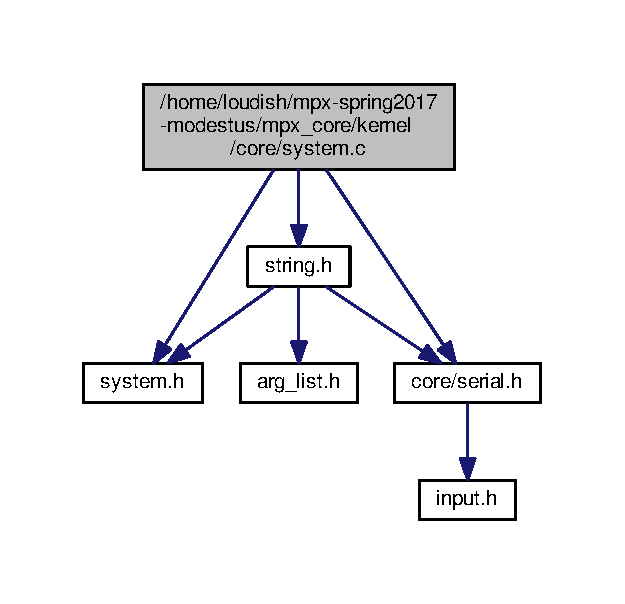
\includegraphics[width=300pt]{system_8c__incl}
\end{center}
\end{figure}
\subsection*{Functions}
\begin{DoxyCompactItemize}
\item 
void \hyperlink{system_8c_abdb09834267dd4a2a0d07d43ca4d230d}{klogv} (const char $\ast$msg)
\item 
void \hyperlink{system_8c_aff8473f901d828d76d3548130731c41d}{kpanic} (const char $\ast$msg)
\end{DoxyCompactItemize}


\subsection{Function Documentation}
\index{system.\+c@{system.\+c}!klogv@{klogv}}
\index{klogv@{klogv}!system.\+c@{system.\+c}}
\subsubsection[{\texorpdfstring{klogv(const char $\ast$msg)}{klogv(const char *msg)}}]{\setlength{\rightskip}{0pt plus 5cm}void klogv (
\begin{DoxyParamCaption}
\item[{const char $\ast$}]{msg}
\end{DoxyParamCaption}
)}\hypertarget{system_8c_abdb09834267dd4a2a0d07d43ca4d230d}{}\label{system_8c_abdb09834267dd4a2a0d07d43ca4d230d}


Definition at line 11 of file system.\+c.



References serial\+\_\+println(), and strcat().



Referenced by kmain(), and kpanic().


\begin{DoxyCode}
12 \{
13   \textcolor{keywordtype}{char} logmsg[64] = \{\textcolor{charliteral}{'\(\backslash\)0'}\}, prefix[] = \textcolor{stringliteral}{"klogv: "};
14   \hyperlink{string_8h_a8908188ae9fc2f05d993257ef001d553}{strcat}(logmsg, prefix);
15   \hyperlink{string_8h_a8908188ae9fc2f05d993257ef001d553}{strcat}(logmsg, msg);
16   \hyperlink{serial_8h_a3514f7abff236a4e00a6c46021ce5e22}{serial\_println}(logmsg);
17 \}
\end{DoxyCode}
\index{system.\+c@{system.\+c}!kpanic@{kpanic}}
\index{kpanic@{kpanic}!system.\+c@{system.\+c}}
\subsubsection[{\texorpdfstring{kpanic(const char $\ast$msg)}{kpanic(const char *msg)}}]{\setlength{\rightskip}{0pt plus 5cm}void kpanic (
\begin{DoxyParamCaption}
\item[{const char $\ast$}]{msg}
\end{DoxyParamCaption}
)}\hypertarget{system_8c_aff8473f901d828d76d3548130731c41d}{}\label{system_8c_aff8473f901d828d76d3548130731c41d}


Definition at line 24 of file system.\+c.



References cli, hlt, klogv(), and strcat().



Referenced by do\+\_\+bounds(), do\+\_\+breakpoint(), do\+\_\+coprocessor(), do\+\_\+coprocessor\+\_\+segment(), do\+\_\+debug(), do\+\_\+device\+\_\+not\+\_\+available(), do\+\_\+divide\+\_\+error(), do\+\_\+double\+\_\+fault(), do\+\_\+general\+\_\+protection(), do\+\_\+invalid\+\_\+op(), do\+\_\+invalid\+\_\+tss(), do\+\_\+nmi(), do\+\_\+overflow(), do\+\_\+page\+\_\+fault(), do\+\_\+segment\+\_\+not\+\_\+present(), do\+\_\+stack\+\_\+segment(), and new\+\_\+frame().


\begin{DoxyCode}
25 \{
26   \hyperlink{system_8h_a68c330e94fe121eba993e5a5973c3162}{cli}(); \textcolor{comment}{//disable interrupts}
27   \textcolor{keywordtype}{char} logmsg[64] = \{\textcolor{charliteral}{'\(\backslash\)0'}\}, prefix[] = \textcolor{stringliteral}{"Panic: "};
28   \hyperlink{string_8h_a8908188ae9fc2f05d993257ef001d553}{strcat}(logmsg, prefix);
29   \hyperlink{string_8h_a8908188ae9fc2f05d993257ef001d553}{strcat}(logmsg, msg);
30   \hyperlink{system_8c_abdb09834267dd4a2a0d07d43ca4d230d}{klogv}(logmsg);
31   \hyperlink{system_8h_a954b0134ce21d80f0efb22c77e821da3}{hlt}(); \textcolor{comment}{//halt}
32 \}
\end{DoxyCode}

\hypertarget{tables_8c}{}\section{/home/loudish/mpx-\/spring2017-\/modestus/mpx\+\_\+core/kernel/core/tables.c File Reference}
\label{tables_8c}\index{/home/loudish/mpx-\/spring2017-\/modestus/mpx\+\_\+core/kernel/core/tables.\+c@{/home/loudish/mpx-\/spring2017-\/modestus/mpx\+\_\+core/kernel/core/tables.\+c}}
{\ttfamily \#include $<$string.\+h$>$}\\*
{\ttfamily \#include $<$core/tables.\+h$>$}\\*
Include dependency graph for tables.\+c\+:\nopagebreak
\begin{figure}[H]
\begin{center}
\leavevmode
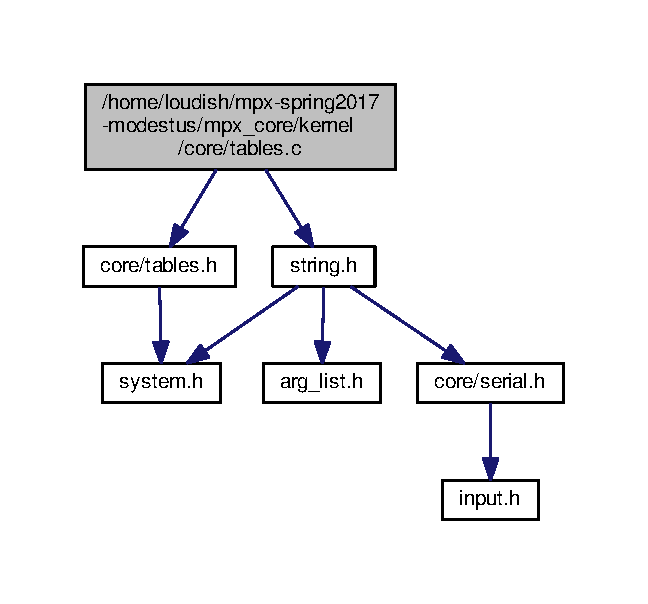
\includegraphics[width=311pt]{tables_8c__incl}
\end{center}
\end{figure}
\subsection*{Functions}
\begin{DoxyCompactItemize}
\item 
void \hyperlink{tables_8c_ab603373c64fb0a6d51482121d0800be4}{write\+\_\+gdt\+\_\+ptr} (\hyperlink{system_8h_a757de76cafbcddaac0d1632902fe4cb8}{u32int}, \hyperlink{system_8h_a7c94ea6f8948649f8d181ae55911eeaf}{size\+\_\+t})
\item 
void \hyperlink{tables_8c_a77fec66a455d3275b67be5c3d7868555}{write\+\_\+idt\+\_\+ptr} (\hyperlink{system_8h_a757de76cafbcddaac0d1632902fe4cb8}{u32int})
\item 
void \hyperlink{tables_8c_a9eca3fe1465f8d7d383551d804853139}{idt\+\_\+set\+\_\+gate} (\hyperlink{system_8h_a1026e682ffdadc1701c42cd44ce9efcf}{u8int} idx, \hyperlink{system_8h_a757de76cafbcddaac0d1632902fe4cb8}{u32int} \hyperlink{tables_8h_ab5763c2b18c825c8b8fba44b2e60ddc1}{base}, \hyperlink{system_8h_a863d9497073aad2b991aeab2211d87af}{u16int} sel, \hyperlink{system_8h_a1026e682ffdadc1701c42cd44ce9efcf}{u8int} \hyperlink{tables_8h_a138dda98fcd4738346af61bcca8cf4b4}{flags})
\item 
void \hyperlink{tables_8c_a35fe413107af682030ab7a4b6dff19b8}{init\+\_\+idt} ()
\item 
void \hyperlink{tables_8c_a0b5aee548c88c40ecb07741be1be2e27}{gdt\+\_\+init\+\_\+entry} (int idx, \hyperlink{system_8h_a757de76cafbcddaac0d1632902fe4cb8}{u32int} \hyperlink{tables_8h_ab5763c2b18c825c8b8fba44b2e60ddc1}{base}, \hyperlink{system_8h_a757de76cafbcddaac0d1632902fe4cb8}{u32int} \hyperlink{tables_8h_a68fd3b4f6c14a331ca9b226cbf122e13}{limit}, \hyperlink{system_8h_a1026e682ffdadc1701c42cd44ce9efcf}{u8int} \hyperlink{tables_8h_a360a726ac0b61d9e4e1be3ad34f80244}{access}, \hyperlink{system_8h_a1026e682ffdadc1701c42cd44ce9efcf}{u8int} \hyperlink{tables_8h_a138dda98fcd4738346af61bcca8cf4b4}{flags})
\item 
void \hyperlink{tables_8c_a86bb50044169930202cc403376ef40c3}{init\+\_\+gdt} ()
\end{DoxyCompactItemize}
\subsection*{Variables}
\begin{DoxyCompactItemize}
\item 
gdt\+\_\+descriptor \hyperlink{tables_8c_aedb4641b02b4a269294e53be7c9b280e}{gdt\+\_\+ptr}
\item 
gdt\+\_\+entry \hyperlink{tables_8c_ac64ff6d00454e0b88d43b55536418288}{gdt\+\_\+entries} \mbox{[}5\mbox{]}
\item 
idt\+\_\+descriptor \hyperlink{tables_8c_a76f617adbc46449bbc39e7b46504b7c4}{idt\+\_\+ptr}
\item 
idt\+\_\+entry \hyperlink{tables_8c_a3c386c59636822ce451be20cc1433a55}{idt\+\_\+entries} \mbox{[}256\mbox{]}
\end{DoxyCompactItemize}


\subsection{Function Documentation}
\index{tables.\+c@{tables.\+c}!gdt\+\_\+init\+\_\+entry@{gdt\+\_\+init\+\_\+entry}}
\index{gdt\+\_\+init\+\_\+entry@{gdt\+\_\+init\+\_\+entry}!tables.\+c@{tables.\+c}}
\subsubsection[{\texorpdfstring{gdt\+\_\+init\+\_\+entry(int idx, u32int base, u32int limit, u8int access, u8int flags)}{gdt_init_entry(int idx, u32int base, u32int limit, u8int access, u8int flags)}}]{\setlength{\rightskip}{0pt plus 5cm}void gdt\+\_\+init\+\_\+entry (
\begin{DoxyParamCaption}
\item[{int}]{idx, }
\item[{{\bf u32int}}]{base, }
\item[{{\bf u32int}}]{limit, }
\item[{{\bf u8int}}]{access, }
\item[{{\bf u8int}}]{flags}
\end{DoxyParamCaption}
)}\hypertarget{tables_8c_a0b5aee548c88c40ecb07741be1be2e27}{}\label{tables_8c_a0b5aee548c88c40ecb07741be1be2e27}


Definition at line 57 of file tables.\+c.



References access, and gdt\+\_\+entries.



Referenced by init\+\_\+gdt().


\begin{DoxyCode}
59 \{
60   gdt\_entry *new\_entry = &\hyperlink{tables_8c_ac64ff6d00454e0b88d43b55536418288}{gdt\_entries}[idx];
61   new\_entry->base\_low  = (\hyperlink{tables_8h_ab5763c2b18c825c8b8fba44b2e60ddc1}{base} & 0xFFFF);
62   new\_entry->base\_mid  = (\hyperlink{tables_8h_ab5763c2b18c825c8b8fba44b2e60ddc1}{base} >> 16) & 0xFF;
63   new\_entry->base\_high = (\hyperlink{tables_8h_ab5763c2b18c825c8b8fba44b2e60ddc1}{base} >> 24) & 0xFF;
64   new\_entry->limit\_low = (\hyperlink{tables_8h_a68fd3b4f6c14a331ca9b226cbf122e13}{limit} & 0xFFFF);
65   new\_entry->flags  = (\hyperlink{tables_8h_a68fd3b4f6c14a331ca9b226cbf122e13}{limit} >> 16) & 0xFF;
66   new\_entry->flags |= \hyperlink{tables_8h_a138dda98fcd4738346af61bcca8cf4b4}{flags} & 0xF0;
67   new\_entry->access = \hyperlink{tables_8h_a360a726ac0b61d9e4e1be3ad34f80244}{access};
68 \}
\end{DoxyCode}
\index{tables.\+c@{tables.\+c}!idt\+\_\+set\+\_\+gate@{idt\+\_\+set\+\_\+gate}}
\index{idt\+\_\+set\+\_\+gate@{idt\+\_\+set\+\_\+gate}!tables.\+c@{tables.\+c}}
\subsubsection[{\texorpdfstring{idt\+\_\+set\+\_\+gate(u8int idx, u32int base, u16int sel, u8int flags)}{idt_set_gate(u8int idx, u32int base, u16int sel, u8int flags)}}]{\setlength{\rightskip}{0pt plus 5cm}void idt\+\_\+set\+\_\+gate (
\begin{DoxyParamCaption}
\item[{{\bf u8int}}]{idx, }
\item[{{\bf u32int}}]{base, }
\item[{{\bf u16int}}]{sel, }
\item[{{\bf u8int}}]{flags}
\end{DoxyParamCaption}
)}\hypertarget{tables_8c_a9eca3fe1465f8d7d383551d804853139}{}\label{tables_8c_a9eca3fe1465f8d7d383551d804853139}


Definition at line 27 of file tables.\+c.



References flags, and idt\+\_\+entries.



Referenced by init\+\_\+irq().


\begin{DoxyCode}
29 \{
30   idt\_entry *new\_entry = &\hyperlink{tables_8c_a3c386c59636822ce451be20cc1433a55}{idt\_entries}[idx];
31   new\_entry->base\_low  = (\hyperlink{tables_8h_ab5763c2b18c825c8b8fba44b2e60ddc1}{base} &  0xFFFF);
32   new\_entry->base\_high = (\hyperlink{tables_8h_ab5763c2b18c825c8b8fba44b2e60ddc1}{base} >> 16) & 0xFFFF;
33   new\_entry->sselect   = sel;
34   new\_entry->zero = 0;
35   new\_entry->flags = \hyperlink{tables_8h_a138dda98fcd4738346af61bcca8cf4b4}{flags};
36 \}
\end{DoxyCode}
\index{tables.\+c@{tables.\+c}!init\+\_\+gdt@{init\+\_\+gdt}}
\index{init\+\_\+gdt@{init\+\_\+gdt}!tables.\+c@{tables.\+c}}
\subsubsection[{\texorpdfstring{init\+\_\+gdt()}{init_gdt()}}]{\setlength{\rightskip}{0pt plus 5cm}void init\+\_\+gdt (
\begin{DoxyParamCaption}
{}
\end{DoxyParamCaption}
)}\hypertarget{tables_8c_a86bb50044169930202cc403376ef40c3}{}\label{tables_8c_a86bb50044169930202cc403376ef40c3}


Definition at line 75 of file tables.\+c.



References gdt\+\_\+entries, gdt\+\_\+init\+\_\+entry(), gdt\+\_\+ptr, limit, and write\+\_\+gdt\+\_\+ptr().



Referenced by kmain().


\begin{DoxyCode}
76 \{
77   \hyperlink{tables_8c_aedb4641b02b4a269294e53be7c9b280e}{gdt\_ptr}.limit = 5 * \textcolor{keyword}{sizeof}(gdt\_entry) - 1;
78   \hyperlink{tables_8c_aedb4641b02b4a269294e53be7c9b280e}{gdt\_ptr}.base  = (\hyperlink{system_8h_a757de76cafbcddaac0d1632902fe4cb8}{u32int}) \hyperlink{tables_8c_ac64ff6d00454e0b88d43b55536418288}{gdt\_entries};
79 
80   \hyperlink{system_8h_a757de76cafbcddaac0d1632902fe4cb8}{u32int} \hyperlink{tables_8h_a68fd3b4f6c14a331ca9b226cbf122e13}{limit} = 0xFFFFFFFF;
81   \hyperlink{tables_8c_a0b5aee548c88c40ecb07741be1be2e27}{gdt\_init\_entry}(0, 0, 0, 0, 0);           \textcolor{comment}{//required null segment}
82   \hyperlink{tables_8c_a0b5aee548c88c40ecb07741be1be2e27}{gdt\_init\_entry}(1, 0, limit, 0x9A, 0xCF); \textcolor{comment}{//code segment}
83   \hyperlink{tables_8c_a0b5aee548c88c40ecb07741be1be2e27}{gdt\_init\_entry}(2, 0, limit, 0x92, 0xCF); \textcolor{comment}{//data segment}
84   \hyperlink{tables_8c_a0b5aee548c88c40ecb07741be1be2e27}{gdt\_init\_entry}(3, 0, limit, 0xFA, 0xCF); \textcolor{comment}{//user mode code segment}
85   \hyperlink{tables_8c_a0b5aee548c88c40ecb07741be1be2e27}{gdt\_init\_entry}(4, 0, limit, 0xF2, 0xCF); \textcolor{comment}{//user mode data segment}
86 
87   \hyperlink{tables_8c_ab603373c64fb0a6d51482121d0800be4}{write\_gdt\_ptr}((\hyperlink{system_8h_a757de76cafbcddaac0d1632902fe4cb8}{u32int}) &\hyperlink{tables_8c_aedb4641b02b4a269294e53be7c9b280e}{gdt\_ptr}, \textcolor{keyword}{sizeof}(gdt\_ptr));
88 \}
\end{DoxyCode}
\index{tables.\+c@{tables.\+c}!init\+\_\+idt@{init\+\_\+idt}}
\index{init\+\_\+idt@{init\+\_\+idt}!tables.\+c@{tables.\+c}}
\subsubsection[{\texorpdfstring{init\+\_\+idt()}{init_idt()}}]{\setlength{\rightskip}{0pt plus 5cm}void init\+\_\+idt (
\begin{DoxyParamCaption}
{}
\end{DoxyParamCaption}
)}\hypertarget{tables_8c_a35fe413107af682030ab7a4b6dff19b8}{}\label{tables_8c_a35fe413107af682030ab7a4b6dff19b8}


Definition at line 43 of file tables.\+c.



References idt\+\_\+entries, idt\+\_\+ptr, memset(), and write\+\_\+idt\+\_\+ptr().



Referenced by kmain().


\begin{DoxyCode}
44 \{
45   \hyperlink{tables_8c_a76f617adbc46449bbc39e7b46504b7c4}{idt\_ptr}.limit = 256*\textcolor{keyword}{sizeof}(idt\_descriptor) - 1;
46   \hyperlink{tables_8c_a76f617adbc46449bbc39e7b46504b7c4}{idt\_ptr}.base  = (\hyperlink{system_8h_a757de76cafbcddaac0d1632902fe4cb8}{u32int})\hyperlink{tables_8c_a3c386c59636822ce451be20cc1433a55}{idt\_entries};
47   \hyperlink{string_8h_ace6ee45c30e71865e6eb635200379db9}{memset}(\hyperlink{tables_8c_a3c386c59636822ce451be20cc1433a55}{idt\_entries}, 0, 256*\textcolor{keyword}{sizeof}(idt\_descriptor));
48   
49   \hyperlink{tables_8c_a77fec66a455d3275b67be5c3d7868555}{write\_idt\_ptr}((\hyperlink{system_8h_a757de76cafbcddaac0d1632902fe4cb8}{u32int})&\hyperlink{tables_8c_a76f617adbc46449bbc39e7b46504b7c4}{idt\_ptr});
50 \}
\end{DoxyCode}
\index{tables.\+c@{tables.\+c}!write\+\_\+gdt\+\_\+ptr@{write\+\_\+gdt\+\_\+ptr}}
\index{write\+\_\+gdt\+\_\+ptr@{write\+\_\+gdt\+\_\+ptr}!tables.\+c@{tables.\+c}}
\subsubsection[{\texorpdfstring{write\+\_\+gdt\+\_\+ptr(u32int, size\+\_\+t)}{write_gdt_ptr(u32int, size_t)}}]{\setlength{\rightskip}{0pt plus 5cm}void write\+\_\+gdt\+\_\+ptr (
\begin{DoxyParamCaption}
\item[{{\bf u32int}}]{, }
\item[{{\bf size\+\_\+t}}]{}
\end{DoxyParamCaption}
)}\hypertarget{tables_8c_ab603373c64fb0a6d51482121d0800be4}{}\label{tables_8c_ab603373c64fb0a6d51482121d0800be4}


Referenced by init\+\_\+gdt().

\index{tables.\+c@{tables.\+c}!write\+\_\+idt\+\_\+ptr@{write\+\_\+idt\+\_\+ptr}}
\index{write\+\_\+idt\+\_\+ptr@{write\+\_\+idt\+\_\+ptr}!tables.\+c@{tables.\+c}}
\subsubsection[{\texorpdfstring{write\+\_\+idt\+\_\+ptr(u32int)}{write_idt_ptr(u32int)}}]{\setlength{\rightskip}{0pt plus 5cm}void write\+\_\+idt\+\_\+ptr (
\begin{DoxyParamCaption}
\item[{{\bf u32int}}]{}
\end{DoxyParamCaption}
)}\hypertarget{tables_8c_a77fec66a455d3275b67be5c3d7868555}{}\label{tables_8c_a77fec66a455d3275b67be5c3d7868555}


Referenced by init\+\_\+idt().



\subsection{Variable Documentation}
\index{tables.\+c@{tables.\+c}!gdt\+\_\+entries@{gdt\+\_\+entries}}
\index{gdt\+\_\+entries@{gdt\+\_\+entries}!tables.\+c@{tables.\+c}}
\subsubsection[{\texorpdfstring{gdt\+\_\+entries}{gdt_entries}}]{\setlength{\rightskip}{0pt plus 5cm}gdt\+\_\+entry gdt\+\_\+entries\mbox{[}5\mbox{]}}\hypertarget{tables_8c_ac64ff6d00454e0b88d43b55536418288}{}\label{tables_8c_ac64ff6d00454e0b88d43b55536418288}


Definition at line 13 of file tables.\+c.



Referenced by gdt\+\_\+init\+\_\+entry(), and init\+\_\+gdt().

\index{tables.\+c@{tables.\+c}!gdt\+\_\+ptr@{gdt\+\_\+ptr}}
\index{gdt\+\_\+ptr@{gdt\+\_\+ptr}!tables.\+c@{tables.\+c}}
\subsubsection[{\texorpdfstring{gdt\+\_\+ptr}{gdt_ptr}}]{\setlength{\rightskip}{0pt plus 5cm}gdt\+\_\+descriptor gdt\+\_\+ptr}\hypertarget{tables_8c_aedb4641b02b4a269294e53be7c9b280e}{}\label{tables_8c_aedb4641b02b4a269294e53be7c9b280e}


Definition at line 12 of file tables.\+c.



Referenced by init\+\_\+gdt().

\index{tables.\+c@{tables.\+c}!idt\+\_\+entries@{idt\+\_\+entries}}
\index{idt\+\_\+entries@{idt\+\_\+entries}!tables.\+c@{tables.\+c}}
\subsubsection[{\texorpdfstring{idt\+\_\+entries}{idt_entries}}]{\setlength{\rightskip}{0pt plus 5cm}idt\+\_\+entry idt\+\_\+entries\mbox{[}256\mbox{]}}\hypertarget{tables_8c_a3c386c59636822ce451be20cc1433a55}{}\label{tables_8c_a3c386c59636822ce451be20cc1433a55}


Definition at line 17 of file tables.\+c.



Referenced by idt\+\_\+set\+\_\+gate(), and init\+\_\+idt().

\index{tables.\+c@{tables.\+c}!idt\+\_\+ptr@{idt\+\_\+ptr}}
\index{idt\+\_\+ptr@{idt\+\_\+ptr}!tables.\+c@{tables.\+c}}
\subsubsection[{\texorpdfstring{idt\+\_\+ptr}{idt_ptr}}]{\setlength{\rightskip}{0pt plus 5cm}idt\+\_\+descriptor idt\+\_\+ptr}\hypertarget{tables_8c_a76f617adbc46449bbc39e7b46504b7c4}{}\label{tables_8c_a76f617adbc46449bbc39e7b46504b7c4}


Definition at line 16 of file tables.\+c.



Referenced by init\+\_\+idt().


\hypertarget{heap_8c}{}\section{/home/loudish/mpx-\/spring2017-\/modestus/mpx\+\_\+core/kernel/mem/heap.c File Reference}
\label{heap_8c}\index{/home/loudish/mpx-\/spring2017-\/modestus/mpx\+\_\+core/kernel/mem/heap.\+c@{/home/loudish/mpx-\/spring2017-\/modestus/mpx\+\_\+core/kernel/mem/heap.\+c}}
{\ttfamily \#include $<$system.\+h$>$}\\*
{\ttfamily \#include $<$string.\+h$>$}\\*
{\ttfamily \#include $<$core/serial.\+h$>$}\\*
{\ttfamily \#include $<$mem/heap.\+h$>$}\\*
{\ttfamily \#include $<$mem/paging.\+h$>$}\\*
Include dependency graph for heap.\+c\+:\nopagebreak
\begin{figure}[H]
\begin{center}
\leavevmode
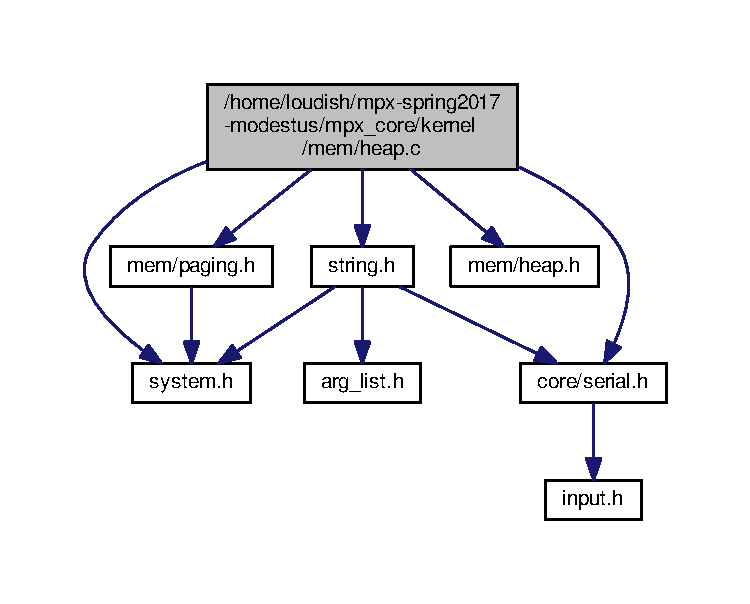
\includegraphics[width=350pt]{heap_8c__incl}
\end{center}
\end{figure}
\subsection*{Functions}
\begin{DoxyCompactItemize}
\item 
\hyperlink{system_8h_a757de76cafbcddaac0d1632902fe4cb8}{u32int} \hyperlink{heap_8c_a014b54e36b61f133f53dd509c461f35e}{\+\_\+kmalloc} (\hyperlink{system_8h_a757de76cafbcddaac0d1632902fe4cb8}{u32int} size, int page\+\_\+align, \hyperlink{system_8h_a757de76cafbcddaac0d1632902fe4cb8}{u32int} $\ast$phys\+\_\+addr)
\item 
\hyperlink{system_8h_a757de76cafbcddaac0d1632902fe4cb8}{u32int} \hyperlink{heap_8c_a15d6a52c5c080c8c7ffc73e336d8e574}{kmalloc} (\hyperlink{system_8h_a757de76cafbcddaac0d1632902fe4cb8}{u32int} size)
\item 
\hyperlink{system_8h_a757de76cafbcddaac0d1632902fe4cb8}{u32int} \hyperlink{heap_8c_a06dae34c7e7c73d518de00212a7c92da}{alloc} (\hyperlink{system_8h_a757de76cafbcddaac0d1632902fe4cb8}{u32int} size, \hyperlink{structheap}{heap} $\ast$h, int align)
\item 
\hyperlink{structheap}{heap} $\ast$ \hyperlink{heap_8c_a686135c02695aef4208f93d4549a15d0}{make\+\_\+heap} (\hyperlink{system_8h_a757de76cafbcddaac0d1632902fe4cb8}{u32int} \hyperlink{tables_8h_ab5763c2b18c825c8b8fba44b2e60ddc1}{base}, \hyperlink{system_8h_a757de76cafbcddaac0d1632902fe4cb8}{u32int} max, \hyperlink{system_8h_a757de76cafbcddaac0d1632902fe4cb8}{u32int} min)
\end{DoxyCompactItemize}
\subsection*{Variables}
\begin{DoxyCompactItemize}
\item 
\hyperlink{structheap}{heap} $\ast$ \hyperlink{heap_8c_a61825456a33b09780a5493c95adcae8a}{kheap} = 0
\item 
\hyperlink{structheap}{heap} $\ast$ \hyperlink{heap_8c_afaac4d3fb801ecbd3c6fe3c995d5cf82}{curr\+\_\+heap} = 0
\item 
\hyperlink{structpage__dir}{page\+\_\+dir} $\ast$ \hyperlink{heap_8c_a61ce943ba80d9dfab89a826cae9ddc4a}{kdir}
\item 
void $\ast$ \hyperlink{heap_8c_a57dfa4d169c6b9c0b4e7352bc0c34366}{end}
\item 
void \hyperlink{heap_8c_a850b19392dca6170001ce200467ab610}{\+\_\+end}
\item 
void \hyperlink{heap_8c_a51f2442fadb8ffd3019f4aeb1b04c4d6}{\+\_\+\+\_\+end}
\item 
\hyperlink{system_8h_a757de76cafbcddaac0d1632902fe4cb8}{u32int} \hyperlink{heap_8c_a6dfa4ef84e115e891b3679e4932b5c49}{phys\+\_\+alloc\+\_\+addr} = (\hyperlink{system_8h_a757de76cafbcddaac0d1632902fe4cb8}{u32int})\&\hyperlink{heap_8c_a57dfa4d169c6b9c0b4e7352bc0c34366}{end}
\end{DoxyCompactItemize}


\subsection{Function Documentation}
\index{heap.\+c@{heap.\+c}!\+\_\+kmalloc@{\+\_\+kmalloc}}
\index{\+\_\+kmalloc@{\+\_\+kmalloc}!heap.\+c@{heap.\+c}}
\subsubsection[{\texorpdfstring{\+\_\+kmalloc(u32int size, int page\+\_\+align, u32int $\ast$phys\+\_\+addr)}{_kmalloc(u32int size, int page_align, u32int *phys_addr)}}]{\setlength{\rightskip}{0pt plus 5cm}{\bf u32int} \+\_\+kmalloc (
\begin{DoxyParamCaption}
\item[{{\bf u32int}}]{size, }
\item[{int}]{page\+\_\+align, }
\item[{{\bf u32int} $\ast$}]{phys\+\_\+addr}
\end{DoxyParamCaption}
)}\hypertarget{heap_8c_a014b54e36b61f133f53dd509c461f35e}{}\label{heap_8c_a014b54e36b61f133f53dd509c461f35e}


Definition at line 24 of file heap.\+c.



References alloc(), page\+\_\+entry\+::frameaddr, get\+\_\+page(), and phys\+\_\+alloc\+\_\+addr.



Referenced by get\+\_\+page(), init\+\_\+paging(), and kmalloc().


\begin{DoxyCode}
25 \{
26   \hyperlink{system_8h_a757de76cafbcddaac0d1632902fe4cb8}{u32int} *addr;
27 
28   \textcolor{comment}{// Allocate on the kernel heap if one has been created}
29   \textcolor{keywordflow}{if} (\hyperlink{heap_8c_a61825456a33b09780a5493c95adcae8a}{kheap} != 0)\{
30     addr = (\hyperlink{system_8h_a757de76cafbcddaac0d1632902fe4cb8}{u32int}*)\hyperlink{heap_8c_a06dae34c7e7c73d518de00212a7c92da}{alloc}(size, \hyperlink{heap_8c_a61825456a33b09780a5493c95adcae8a}{kheap}, page\_align);
31     \textcolor{keywordflow}{if} (phys\_addr)\{
32       \hyperlink{structpage__entry}{page\_entry} *page = \hyperlink{paging_8h_a69b165b3d1adf3aeaae126ca7a5aac3e}{get\_page}((\hyperlink{system_8h_a757de76cafbcddaac0d1632902fe4cb8}{u32int})addr, \hyperlink{heap_8c_a61ce943ba80d9dfab89a826cae9ddc4a}{kdir}, 0);
33       *phys\_addr = (page->\hyperlink{structpage__entry_a68a6dc54a7ab6f7fb1a068476190bf67}{frameaddr}*0x1000) + ((\hyperlink{system_8h_a757de76cafbcddaac0d1632902fe4cb8}{u32int})addr & 0xFFF);
34     \}
35     \textcolor{keywordflow}{return} (\hyperlink{system_8h_a757de76cafbcddaac0d1632902fe4cb8}{u32int})addr;
36   \}
37   \textcolor{comment}{// Else, allocate directly from physical memory}
38   \textcolor{keywordflow}{else} \{
39     \textcolor{keywordflow}{if} (page\_align && (\hyperlink{heap_8c_a6dfa4ef84e115e891b3679e4932b5c49}{phys\_alloc\_addr} & 0xFFFFF000))\{
40       \hyperlink{heap_8c_a6dfa4ef84e115e891b3679e4932b5c49}{phys\_alloc\_addr} &= 0xFFFFF000;
41       \hyperlink{heap_8c_a6dfa4ef84e115e891b3679e4932b5c49}{phys\_alloc\_addr} += 0x1000;
42     \}
43     addr = (\hyperlink{system_8h_a757de76cafbcddaac0d1632902fe4cb8}{u32int}*)\hyperlink{heap_8c_a6dfa4ef84e115e891b3679e4932b5c49}{phys\_alloc\_addr};
44     \textcolor{keywordflow}{if} (phys\_addr)\{
45       *phys\_addr = \hyperlink{heap_8c_a6dfa4ef84e115e891b3679e4932b5c49}{phys\_alloc\_addr};
46     \}
47     \hyperlink{heap_8c_a6dfa4ef84e115e891b3679e4932b5c49}{phys\_alloc\_addr} += size;
48     \textcolor{keywordflow}{return} (\hyperlink{system_8h_a757de76cafbcddaac0d1632902fe4cb8}{u32int})addr;
49   \}
50 \}
\end{DoxyCode}
\index{heap.\+c@{heap.\+c}!alloc@{alloc}}
\index{alloc@{alloc}!heap.\+c@{heap.\+c}}
\subsubsection[{\texorpdfstring{alloc(u32int size, heap $\ast$h, int align)}{alloc(u32int size, heap *h, int align)}}]{\setlength{\rightskip}{0pt plus 5cm}{\bf u32int} alloc (
\begin{DoxyParamCaption}
\item[{{\bf u32int}}]{size, }
\item[{{\bf heap} $\ast$}]{h, }
\item[{int}]{align}
\end{DoxyParamCaption}
)}\hypertarget{heap_8c_a06dae34c7e7c73d518de00212a7c92da}{}\label{heap_8c_a06dae34c7e7c73d518de00212a7c92da}


Definition at line 57 of file heap.\+c.



References base, K\+H\+E\+A\+P\+\_\+\+B\+A\+SE, K\+H\+E\+A\+P\+\_\+\+M\+IN, no\+\_\+warn, and serial\+\_\+println().



Referenced by \+\_\+kmalloc().


\begin{DoxyCode}
58 \{
59   \hyperlink{system_8h_ab3bb695e7817363c7bdb781f214e83a2}{no\_warn}(size||align||h);
60   \textcolor{keyword}{static} \hyperlink{system_8h_a757de76cafbcddaac0d1632902fe4cb8}{u32int} heap\_addr = \hyperlink{heap_8h_a15073b9742f7e29d8174509197eb4ab9}{KHEAP\_BASE};
61 
62   \hyperlink{system_8h_a757de76cafbcddaac0d1632902fe4cb8}{u32int} \hyperlink{tables_8h_ab5763c2b18c825c8b8fba44b2e60ddc1}{base} = heap\_addr;
63   heap\_addr += size;
64 
65   \textcolor{keywordflow}{if} (heap\_addr > \hyperlink{heap_8h_a15073b9742f7e29d8174509197eb4ab9}{KHEAP\_BASE} + \hyperlink{heap_8h_aee52619f74498ad224eb8e4354b89e40}{KHEAP\_MIN})
66     \hyperlink{serial_8h_a3514f7abff236a4e00a6c46021ce5e22}{serial\_println}(\textcolor{stringliteral}{"Heap is full!"});
67 
68   \textcolor{keywordflow}{return} \hyperlink{tables_8h_ab5763c2b18c825c8b8fba44b2e60ddc1}{base};
69 \}
\end{DoxyCode}
\index{heap.\+c@{heap.\+c}!kmalloc@{kmalloc}}
\index{kmalloc@{kmalloc}!heap.\+c@{heap.\+c}}
\subsubsection[{\texorpdfstring{kmalloc(u32int size)}{kmalloc(u32int size)}}]{\setlength{\rightskip}{0pt plus 5cm}{\bf u32int} kmalloc (
\begin{DoxyParamCaption}
\item[{{\bf u32int}}]{size}
\end{DoxyParamCaption}
)}\hypertarget{heap_8c_a15d6a52c5c080c8c7ffc73e336d8e574}{}\label{heap_8c_a15d6a52c5c080c8c7ffc73e336d8e574}


Definition at line 52 of file heap.\+c.



References \+\_\+kmalloc().



Referenced by init\+\_\+paging(), make\+\_\+heap(), and sys\+\_\+alloc\+\_\+mem().


\begin{DoxyCode}
53 \{
54   \textcolor{keywordflow}{return} \hyperlink{heap_8c_a014b54e36b61f133f53dd509c461f35e}{\_kmalloc}(size,0,0);
55 \}
\end{DoxyCode}
\index{heap.\+c@{heap.\+c}!make\+\_\+heap@{make\+\_\+heap}}
\index{make\+\_\+heap@{make\+\_\+heap}!heap.\+c@{heap.\+c}}
\subsubsection[{\texorpdfstring{make\+\_\+heap(u32int base, u32int max, u32int min)}{make_heap(u32int base, u32int max, u32int min)}}]{\setlength{\rightskip}{0pt plus 5cm}{\bf heap}$\ast$ make\+\_\+heap (
\begin{DoxyParamCaption}
\item[{{\bf u32int}}]{base, }
\item[{{\bf u32int}}]{max, }
\item[{{\bf u32int}}]{min}
\end{DoxyParamCaption}
)}\hypertarget{heap_8c_a686135c02695aef4208f93d4549a15d0}{}\label{heap_8c_a686135c02695aef4208f93d4549a15d0}


Definition at line 71 of file heap.\+c.



References kmalloc(), and no\+\_\+warn.



Referenced by init\+\_\+paging().


\begin{DoxyCode}
72 \{  
73   \hyperlink{system_8h_ab3bb695e7817363c7bdb781f214e83a2}{no\_warn}(\hyperlink{tables_8h_ab5763c2b18c825c8b8fba44b2e60ddc1}{base}||max||min);
74   \textcolor{keywordflow}{return} (\hyperlink{structheap}{heap}*)\hyperlink{heap_8c_a15d6a52c5c080c8c7ffc73e336d8e574}{kmalloc}(\textcolor{keyword}{sizeof}(\hyperlink{structheap}{heap}));
75 \}
\end{DoxyCode}


\subsection{Variable Documentation}
\index{heap.\+c@{heap.\+c}!\+\_\+\+\_\+end@{\+\_\+\+\_\+end}}
\index{\+\_\+\+\_\+end@{\+\_\+\+\_\+end}!heap.\+c@{heap.\+c}}
\subsubsection[{\texorpdfstring{\+\_\+\+\_\+end}{__end}}]{\setlength{\rightskip}{0pt plus 5cm}void \+\_\+\+\_\+end}\hypertarget{heap_8c_a51f2442fadb8ffd3019f4aeb1b04c4d6}{}\label{heap_8c_a51f2442fadb8ffd3019f4aeb1b04c4d6}
\index{heap.\+c@{heap.\+c}!\+\_\+end@{\+\_\+end}}
\index{\+\_\+end@{\+\_\+end}!heap.\+c@{heap.\+c}}
\subsubsection[{\texorpdfstring{\+\_\+end}{_end}}]{\setlength{\rightskip}{0pt plus 5cm}void \+\_\+end}\hypertarget{heap_8c_a850b19392dca6170001ce200467ab610}{}\label{heap_8c_a850b19392dca6170001ce200467ab610}
\index{heap.\+c@{heap.\+c}!curr\+\_\+heap@{curr\+\_\+heap}}
\index{curr\+\_\+heap@{curr\+\_\+heap}!heap.\+c@{heap.\+c}}
\subsubsection[{\texorpdfstring{curr\+\_\+heap}{curr_heap}}]{\setlength{\rightskip}{0pt plus 5cm}{\bf heap}$\ast$ curr\+\_\+heap = 0}\hypertarget{heap_8c_afaac4d3fb801ecbd3c6fe3c995d5cf82}{}\label{heap_8c_afaac4d3fb801ecbd3c6fe3c995d5cf82}


Definition at line 15 of file heap.\+c.

\index{heap.\+c@{heap.\+c}!end@{end}}
\index{end@{end}!heap.\+c@{heap.\+c}}
\subsubsection[{\texorpdfstring{end}{end}}]{\setlength{\rightskip}{0pt plus 5cm}void$\ast$ end}\hypertarget{heap_8c_a57dfa4d169c6b9c0b4e7352bc0c34366}{}\label{heap_8c_a57dfa4d169c6b9c0b4e7352bc0c34366}
\index{heap.\+c@{heap.\+c}!kdir@{kdir}}
\index{kdir@{kdir}!heap.\+c@{heap.\+c}}
\subsubsection[{\texorpdfstring{kdir}{kdir}}]{\setlength{\rightskip}{0pt plus 5cm}{\bf page\+\_\+dir}$\ast$ kdir}\hypertarget{heap_8c_a61ce943ba80d9dfab89a826cae9ddc4a}{}\label{heap_8c_a61ce943ba80d9dfab89a826cae9ddc4a}


Definition at line 21 of file paging.\+c.

\index{heap.\+c@{heap.\+c}!kheap@{kheap}}
\index{kheap@{kheap}!heap.\+c@{heap.\+c}}
\subsubsection[{\texorpdfstring{kheap}{kheap}}]{\setlength{\rightskip}{0pt plus 5cm}{\bf heap}$\ast$ kheap = 0}\hypertarget{heap_8c_a61825456a33b09780a5493c95adcae8a}{}\label{heap_8c_a61825456a33b09780a5493c95adcae8a}


Definition at line 14 of file heap.\+c.

\index{heap.\+c@{heap.\+c}!phys\+\_\+alloc\+\_\+addr@{phys\+\_\+alloc\+\_\+addr}}
\index{phys\+\_\+alloc\+\_\+addr@{phys\+\_\+alloc\+\_\+addr}!heap.\+c@{heap.\+c}}
\subsubsection[{\texorpdfstring{phys\+\_\+alloc\+\_\+addr}{phys_alloc_addr}}]{\setlength{\rightskip}{0pt plus 5cm}{\bf u32int} phys\+\_\+alloc\+\_\+addr = ({\bf u32int})\&{\bf end}}\hypertarget{heap_8c_a6dfa4ef84e115e891b3679e4932b5c49}{}\label{heap_8c_a6dfa4ef84e115e891b3679e4932b5c49}


Definition at line 22 of file heap.\+c.



Referenced by \+\_\+kmalloc(), and init\+\_\+paging().


\hypertarget{paging_8c}{}\section{/home/loudish/mpx-\/spring2017-\/modestus/mpx\+\_\+core/kernel/mem/paging.c File Reference}
\label{paging_8c}\index{/home/loudish/mpx-\/spring2017-\/modestus/mpx\+\_\+core/kernel/mem/paging.\+c@{/home/loudish/mpx-\/spring2017-\/modestus/mpx\+\_\+core/kernel/mem/paging.\+c}}
{\ttfamily \#include $<$system.\+h$>$}\\*
{\ttfamily \#include $<$string.\+h$>$}\\*
{\ttfamily \#include \char`\"{}mem/heap.\+h\char`\"{}}\\*
{\ttfamily \#include \char`\"{}mem/paging.\+h\char`\"{}}\\*
Include dependency graph for paging.\+c\+:\nopagebreak
\begin{figure}[H]
\begin{center}
\leavevmode
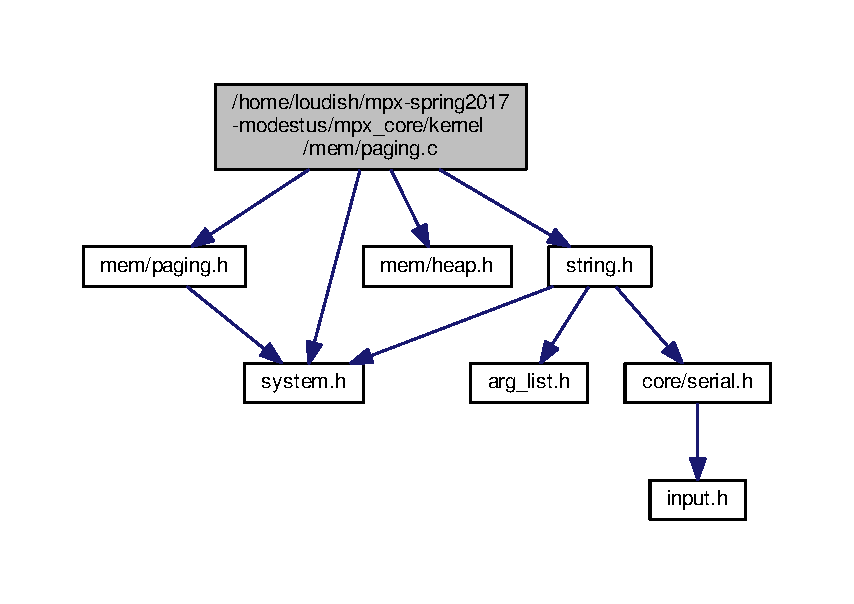
\includegraphics[width=350pt]{paging_8c__incl}
\end{center}
\end{figure}
\subsection*{Functions}
\begin{DoxyCompactItemize}
\item 
void \hyperlink{paging_8c_a70101fc152ff58caafbe36ab391a9a68}{set\+\_\+bit} (\hyperlink{system_8h_a757de76cafbcddaac0d1632902fe4cb8}{u32int} addr)
\item 
void \hyperlink{paging_8c_adcef508c82c20a032508f871e79e1b92}{clear\+\_\+bit} (\hyperlink{system_8h_a757de76cafbcddaac0d1632902fe4cb8}{u32int} addr)
\item 
\hyperlink{system_8h_a757de76cafbcddaac0d1632902fe4cb8}{u32int} \hyperlink{paging_8c_a317b4797bc81f65bd01cfa190800ecdd}{get\+\_\+bit} (\hyperlink{system_8h_a757de76cafbcddaac0d1632902fe4cb8}{u32int} addr)
\item 
\hyperlink{system_8h_a757de76cafbcddaac0d1632902fe4cb8}{u32int} \hyperlink{paging_8c_abe201f9294ab23125146fff36fe95187}{find\+\_\+free} ()
\item 
\hyperlink{structpage__entry}{page\+\_\+entry} $\ast$ \hyperlink{paging_8c_a69b165b3d1adf3aeaae126ca7a5aac3e}{get\+\_\+page} (\hyperlink{system_8h_a757de76cafbcddaac0d1632902fe4cb8}{u32int} addr, \hyperlink{structpage__dir}{page\+\_\+dir} $\ast$dir, int make\+\_\+table)
\item 
void \hyperlink{paging_8c_a919b727f386797a8b9d8eceb5c4e7313}{init\+\_\+paging} ()
\item 
void \hyperlink{paging_8c_a31e6c585cbda542534f1b0fc83e40689}{load\+\_\+page\+\_\+dir} (\hyperlink{structpage__dir}{page\+\_\+dir} $\ast$new\+\_\+dir)
\item 
void \hyperlink{paging_8c_a04bce9da2c1d7c59f6efd8e4d9b54db7}{new\+\_\+frame} (\hyperlink{structpage__entry}{page\+\_\+entry} $\ast$page)
\end{DoxyCompactItemize}
\subsection*{Variables}
\begin{DoxyCompactItemize}
\item 
\hyperlink{system_8h_a757de76cafbcddaac0d1632902fe4cb8}{u32int} \hyperlink{paging_8c_abf8475f59bfb67fac4b6b5a254dfe56d}{mem\+\_\+size} = 0x4000000
\item 
\hyperlink{system_8h_a757de76cafbcddaac0d1632902fe4cb8}{u32int} \hyperlink{paging_8c_a1cc472551ec40b65eef931fde01054e7}{page\+\_\+size} = 0x1000
\item 
\hyperlink{system_8h_a757de76cafbcddaac0d1632902fe4cb8}{u32int} \hyperlink{paging_8c_abf36580d5618820f15388083c9313e60}{nframes}
\item 
\hyperlink{system_8h_a757de76cafbcddaac0d1632902fe4cb8}{u32int} $\ast$ \hyperlink{paging_8c_a76492529572a1a20a06076ac40d66b29}{frames}
\item 
\hyperlink{structpage__dir}{page\+\_\+dir} $\ast$ \hyperlink{paging_8c_a61ce943ba80d9dfab89a826cae9ddc4a}{kdir} = 0
\item 
\hyperlink{structpage__dir}{page\+\_\+dir} $\ast$ \hyperlink{paging_8c_af7da380833e92d5c7d3c3db41484713b}{cdir} = 0
\item 
\hyperlink{system_8h_a757de76cafbcddaac0d1632902fe4cb8}{u32int} \hyperlink{paging_8c_a6dfa4ef84e115e891b3679e4932b5c49}{phys\+\_\+alloc\+\_\+addr}
\item 
\hyperlink{structheap}{heap} $\ast$ \hyperlink{paging_8c_a61825456a33b09780a5493c95adcae8a}{kheap}
\end{DoxyCompactItemize}


\subsection{Function Documentation}
\index{paging.\+c@{paging.\+c}!clear\+\_\+bit@{clear\+\_\+bit}}
\index{clear\+\_\+bit@{clear\+\_\+bit}!paging.\+c@{paging.\+c}}
\subsubsection[{\texorpdfstring{clear\+\_\+bit(u32int addr)}{clear_bit(u32int addr)}}]{\setlength{\rightskip}{0pt plus 5cm}void clear\+\_\+bit (
\begin{DoxyParamCaption}
\item[{{\bf u32int}}]{addr}
\end{DoxyParamCaption}
)}\hypertarget{paging_8c_adcef508c82c20a032508f871e79e1b92}{}\label{paging_8c_adcef508c82c20a032508f871e79e1b92}


Definition at line 44 of file paging.\+c.



References frames, and page\+\_\+size.


\begin{DoxyCode}
45 \{
46   \hyperlink{system_8h_a757de76cafbcddaac0d1632902fe4cb8}{u32int} frame  = addr/\hyperlink{paging_8c_a1cc472551ec40b65eef931fde01054e7}{page\_size};
47   \hyperlink{system_8h_a757de76cafbcddaac0d1632902fe4cb8}{u32int} index  = frame/32;
48   \hyperlink{system_8h_a757de76cafbcddaac0d1632902fe4cb8}{u32int} offset = frame%32;
49   \hyperlink{paging_8c_a76492529572a1a20a06076ac40d66b29}{frames}[index] &= ~(1 << offset);
50 \}
\end{DoxyCode}
\index{paging.\+c@{paging.\+c}!find\+\_\+free@{find\+\_\+free}}
\index{find\+\_\+free@{find\+\_\+free}!paging.\+c@{paging.\+c}}
\subsubsection[{\texorpdfstring{find\+\_\+free()}{find_free()}}]{\setlength{\rightskip}{0pt plus 5cm}{\bf u32int} find\+\_\+free (
\begin{DoxyParamCaption}
{}
\end{DoxyParamCaption}
)}\hypertarget{paging_8c_abe201f9294ab23125146fff36fe95187}{}\label{paging_8c_abe201f9294ab23125146fff36fe95187}


Definition at line 68 of file paging.\+c.



References frames, and nframes.



Referenced by new\+\_\+frame().


\begin{DoxyCode}
69 \{
70   \hyperlink{system_8h_a757de76cafbcddaac0d1632902fe4cb8}{u32int} i,j;
71   \textcolor{keywordflow}{for} (i=0; i<\hyperlink{paging_8c_abf36580d5618820f15388083c9313e60}{nframes}/32; i++)
72     \textcolor{keywordflow}{if} (\hyperlink{paging_8c_a76492529572a1a20a06076ac40d66b29}{frames}[i] != 0xFFFFFFFF) \textcolor{comment}{//if frame not full}
73       \textcolor{keywordflow}{for} (j=0; j<32; j++) \textcolor{comment}{//find first free bit}
74     \textcolor{keywordflow}{if} (!(\hyperlink{paging_8c_a76492529572a1a20a06076ac40d66b29}{frames}[i] & (1 << j)))
75       \textcolor{keywordflow}{return} i*32+j;
76 
77   \textcolor{keywordflow}{return} -1; \textcolor{comment}{//no free frames}
78 \}
\end{DoxyCode}
\index{paging.\+c@{paging.\+c}!get\+\_\+bit@{get\+\_\+bit}}
\index{get\+\_\+bit@{get\+\_\+bit}!paging.\+c@{paging.\+c}}
\subsubsection[{\texorpdfstring{get\+\_\+bit(u32int addr)}{get_bit(u32int addr)}}]{\setlength{\rightskip}{0pt plus 5cm}{\bf u32int} get\+\_\+bit (
\begin{DoxyParamCaption}
\item[{{\bf u32int}}]{addr}
\end{DoxyParamCaption}
)}\hypertarget{paging_8c_a317b4797bc81f65bd01cfa190800ecdd}{}\label{paging_8c_a317b4797bc81f65bd01cfa190800ecdd}


Definition at line 56 of file paging.\+c.



References frames, and page\+\_\+size.


\begin{DoxyCode}
57 \{
58   \hyperlink{system_8h_a757de76cafbcddaac0d1632902fe4cb8}{u32int} frame  = addr/\hyperlink{paging_8c_a1cc472551ec40b65eef931fde01054e7}{page\_size};
59   \hyperlink{system_8h_a757de76cafbcddaac0d1632902fe4cb8}{u32int} index  = frame/32;
60   \hyperlink{system_8h_a757de76cafbcddaac0d1632902fe4cb8}{u32int} offset = frame%32;
61   \textcolor{keywordflow}{return} (\hyperlink{paging_8c_a76492529572a1a20a06076ac40d66b29}{frames}[index] & (1 << offset));  
62 \}
\end{DoxyCode}
\index{paging.\+c@{paging.\+c}!get\+\_\+page@{get\+\_\+page}}
\index{get\+\_\+page@{get\+\_\+page}!paging.\+c@{paging.\+c}}
\subsubsection[{\texorpdfstring{get\+\_\+page(u32int addr, page\+\_\+dir $\ast$dir, int make\+\_\+table)}{get_page(u32int addr, page_dir *dir, int make_table)}}]{\setlength{\rightskip}{0pt plus 5cm}{\bf page\+\_\+entry}$\ast$ get\+\_\+page (
\begin{DoxyParamCaption}
\item[{{\bf u32int}}]{addr, }
\item[{{\bf page\+\_\+dir} $\ast$}]{dir, }
\item[{int}]{make\+\_\+table}
\end{DoxyParamCaption}
)}\hypertarget{paging_8c_a69b165b3d1adf3aeaae126ca7a5aac3e}{}\label{paging_8c_a69b165b3d1adf3aeaae126ca7a5aac3e}


Definition at line 85 of file paging.\+c.



References \+\_\+kmalloc(), page\+\_\+size, page\+\_\+table\+::pages, page\+\_\+dir\+::tables, and page\+\_\+dir\+::tables\+\_\+phys.



Referenced by \+\_\+kmalloc(), and init\+\_\+paging().


\begin{DoxyCode}
86 \{
87   \hyperlink{system_8h_a757de76cafbcddaac0d1632902fe4cb8}{u32int} phys\_addr;
88   \hyperlink{system_8h_a757de76cafbcddaac0d1632902fe4cb8}{u32int} index = addr / \hyperlink{paging_8c_a1cc472551ec40b65eef931fde01054e7}{page\_size} / 1024;
89   \hyperlink{system_8h_a757de76cafbcddaac0d1632902fe4cb8}{u32int} offset = addr / \hyperlink{paging_8c_a1cc472551ec40b65eef931fde01054e7}{page\_size} % 1024;
90   
91   \textcolor{comment}{//return it if it exists}
92   \textcolor{keywordflow}{if} (dir->\hyperlink{structpage__dir_ac89434e3fccabfe9481ea77fdda82faf}{tables}[index])
93     \textcolor{keywordflow}{return} &dir->\hyperlink{structpage__dir_ac89434e3fccabfe9481ea77fdda82faf}{tables}[index]->\hyperlink{structpage__table_aa066e0fa847ce2fafb6a2feddfa340ff}{pages}[offset];
94   
95   \textcolor{comment}{//create it}
96   \textcolor{keywordflow}{else} \textcolor{keywordflow}{if} (make\_table)\{
97     dir->\hyperlink{structpage__dir_ac89434e3fccabfe9481ea77fdda82faf}{tables}[index] = (\hyperlink{structpage__table}{page\_table}*)\hyperlink{heap_8h_a9bfb8053c2382598ef5b2175f475d49a}{\_kmalloc}(\textcolor{keyword}{sizeof}(
      \hyperlink{structpage__table}{page\_table}), 1, &phys\_addr);
98     dir->\hyperlink{structpage__dir_a7336b695acaf516613dda626129129d0}{tables\_phys}[index] = phys\_addr | 0x7; \textcolor{comment}{//enable present, writable}
99     \textcolor{keywordflow}{return} &dir->\hyperlink{structpage__dir_ac89434e3fccabfe9481ea77fdda82faf}{tables}[index]->\hyperlink{structpage__table_aa066e0fa847ce2fafb6a2feddfa340ff}{pages}[offset];
100   \}
101   \textcolor{keywordflow}{else} \textcolor{keywordflow}{return} 0;
102 \}
\end{DoxyCode}
\index{paging.\+c@{paging.\+c}!init\+\_\+paging@{init\+\_\+paging}}
\index{init\+\_\+paging@{init\+\_\+paging}!paging.\+c@{paging.\+c}}
\subsubsection[{\texorpdfstring{init\+\_\+paging()}{init_paging()}}]{\setlength{\rightskip}{0pt plus 5cm}void init\+\_\+paging (
\begin{DoxyParamCaption}
{}
\end{DoxyParamCaption}
)}\hypertarget{paging_8c_a919b727f386797a8b9d8eceb5c4e7313}{}\label{paging_8c_a919b727f386797a8b9d8eceb5c4e7313}


Definition at line 111 of file paging.\+c.



References \+\_\+kmalloc(), frames, get\+\_\+page(), K\+H\+E\+A\+P\+\_\+\+B\+A\+SE, K\+H\+E\+A\+P\+\_\+\+M\+IN, K\+H\+E\+A\+P\+\_\+\+S\+I\+ZE, kmalloc(), load\+\_\+page\+\_\+dir(), make\+\_\+heap(), mem\+\_\+size, memset(), new\+\_\+frame(), nframes, P\+A\+G\+E\+\_\+\+S\+I\+ZE, page\+\_\+size, and phys\+\_\+alloc\+\_\+addr.



Referenced by kmain().


\begin{DoxyCode}
112 \{
113   \textcolor{comment}{//create frame bitmap}
114   \hyperlink{paging_8c_abf36580d5618820f15388083c9313e60}{nframes} = (\hyperlink{system_8h_a757de76cafbcddaac0d1632902fe4cb8}{u32int})(\hyperlink{paging_8c_abf8475f59bfb67fac4b6b5a254dfe56d}{mem\_size}/\hyperlink{paging_8c_a1cc472551ec40b65eef931fde01054e7}{page\_size});
115   \hyperlink{paging_8c_a76492529572a1a20a06076ac40d66b29}{frames} = (\hyperlink{system_8h_a757de76cafbcddaac0d1632902fe4cb8}{u32int}*)\hyperlink{heap_8h_a15d6a52c5c080c8c7ffc73e336d8e574}{kmalloc}(\hyperlink{paging_8c_abf36580d5618820f15388083c9313e60}{nframes}/32);
116   \hyperlink{string_8h_ace6ee45c30e71865e6eb635200379db9}{memset}(\hyperlink{paging_8c_a76492529572a1a20a06076ac40d66b29}{frames}, 0, \hyperlink{paging_8c_abf36580d5618820f15388083c9313e60}{nframes}/32);
117 
118   \textcolor{comment}{//create kernel directory}
119   \hyperlink{paging_8c_a61ce943ba80d9dfab89a826cae9ddc4a}{kdir} = (\hyperlink{structpage__dir}{page\_dir}*)\hyperlink{heap_8h_a9bfb8053c2382598ef5b2175f475d49a}{\_kmalloc}(\textcolor{keyword}{sizeof}(\hyperlink{structpage__dir}{page\_dir}), 1, 0); \textcolor{comment}{//page aligned}
120   \hyperlink{string_8h_ace6ee45c30e71865e6eb635200379db9}{memset}(\hyperlink{paging_8c_a61ce943ba80d9dfab89a826cae9ddc4a}{kdir}, 0, \textcolor{keyword}{sizeof}(\hyperlink{structpage__dir}{page\_dir}));
121 
122   \textcolor{comment}{//get pages for kernel heap}
123   \hyperlink{system_8h_a757de76cafbcddaac0d1632902fe4cb8}{u32int} i = 0x0;
124   \textcolor{keywordflow}{for}(i=\hyperlink{heap_8h_a15073b9742f7e29d8174509197eb4ab9}{KHEAP\_BASE}; i<(\hyperlink{heap_8h_a15073b9742f7e29d8174509197eb4ab9}{KHEAP\_BASE}+\hyperlink{heap_8h_aee52619f74498ad224eb8e4354b89e40}{KHEAP\_MIN}); i+=1)\{
125     \hyperlink{paging_8c_a69b165b3d1adf3aeaae126ca7a5aac3e}{get\_page}(i,\hyperlink{paging_8c_a61ce943ba80d9dfab89a826cae9ddc4a}{kdir},1);
126   \}
127 
128   \textcolor{comment}{//perform identity mapping of used memory}
129   \textcolor{comment}{//note: placement\_addr gets incremented in get\_page,}
130   \textcolor{comment}{//so we're mapping the first frames as well}
131   i = 0x0;
132   \textcolor{keywordflow}{while} (i < (\hyperlink{paging_8c_a6dfa4ef84e115e891b3679e4932b5c49}{phys\_alloc\_addr}+0x10000))\{
133     \hyperlink{paging_8c_a04bce9da2c1d7c59f6efd8e4d9b54db7}{new\_frame}(\hyperlink{paging_8c_a69b165b3d1adf3aeaae126ca7a5aac3e}{get\_page}(i,\hyperlink{paging_8c_a61ce943ba80d9dfab89a826cae9ddc4a}{kdir},1));
134     i += \hyperlink{paging_8c_a1cc472551ec40b65eef931fde01054e7}{page\_size};
135   \}
136 
137   \textcolor{comment}{//allocate heap frames now that the placement addr has increased.}
138   \textcolor{comment}{//placement addr increases here for heap}
139   \textcolor{keywordflow}{for}(i=\hyperlink{heap_8h_a15073b9742f7e29d8174509197eb4ab9}{KHEAP\_BASE}; i<(\hyperlink{heap_8h_a15073b9742f7e29d8174509197eb4ab9}{KHEAP\_BASE}+\hyperlink{heap_8h_aee52619f74498ad224eb8e4354b89e40}{KHEAP\_MIN});i+=
      \hyperlink{paging_8h_a7d467c1d283fdfa1f2081ba1e0d01b6e}{PAGE\_SIZE})\{
140     \hyperlink{paging_8c_a04bce9da2c1d7c59f6efd8e4d9b54db7}{new\_frame}(\hyperlink{paging_8c_a69b165b3d1adf3aeaae126ca7a5aac3e}{get\_page}(i,\hyperlink{paging_8c_a61ce943ba80d9dfab89a826cae9ddc4a}{kdir},1));
141   \}
142 
143   \textcolor{comment}{//load the kernel page directory; enable paging}
144   \hyperlink{paging_8c_a31e6c585cbda542534f1b0fc83e40689}{load\_page\_dir}(\hyperlink{paging_8c_a61ce943ba80d9dfab89a826cae9ddc4a}{kdir});
145 
146   \textcolor{comment}{//setup the kernel heap}
147   \hyperlink{paging_8c_a61825456a33b09780a5493c95adcae8a}{kheap} = \hyperlink{heap_8h_a686135c02695aef4208f93d4549a15d0}{make\_heap}(\hyperlink{heap_8h_a15073b9742f7e29d8174509197eb4ab9}{KHEAP\_BASE}, \hyperlink{heap_8h_a0f2696767a10e6efffc64e9b459c4ea6}{KHEAP\_SIZE}, 
      \hyperlink{heap_8h_a15073b9742f7e29d8174509197eb4ab9}{KHEAP\_BASE}+\hyperlink{heap_8h_aee52619f74498ad224eb8e4354b89e40}{KHEAP\_MIN});
148 \}
\end{DoxyCode}
\index{paging.\+c@{paging.\+c}!load\+\_\+page\+\_\+dir@{load\+\_\+page\+\_\+dir}}
\index{load\+\_\+page\+\_\+dir@{load\+\_\+page\+\_\+dir}!paging.\+c@{paging.\+c}}
\subsubsection[{\texorpdfstring{load\+\_\+page\+\_\+dir(page\+\_\+dir $\ast$new\+\_\+dir)}{load_page_dir(page_dir *new_dir)}}]{\setlength{\rightskip}{0pt plus 5cm}void load\+\_\+page\+\_\+dir (
\begin{DoxyParamCaption}
\item[{{\bf page\+\_\+dir} $\ast$}]{new\+\_\+dir}
\end{DoxyParamCaption}
)}\hypertarget{paging_8c_a31e6c585cbda542534f1b0fc83e40689}{}\label{paging_8c_a31e6c585cbda542534f1b0fc83e40689}


Definition at line 158 of file paging.\+c.



References page\+\_\+dir\+::tables\+\_\+phys.



Referenced by init\+\_\+paging().


\begin{DoxyCode}
159 \{
160   \hyperlink{paging_8c_af7da380833e92d5c7d3c3db41484713b}{cdir} = new\_dir;
161   \textcolor{keyword}{asm} \textcolor{keyword}{volatile} (\textcolor{stringliteral}{"mov %0,%%cr3"}:: \textcolor{stringliteral}{"b"}(&\hyperlink{paging_8c_af7da380833e92d5c7d3c3db41484713b}{cdir}->\hyperlink{structpage__dir_a7336b695acaf516613dda626129129d0}{tables\_phys}[0]));
162   \hyperlink{system_8h_a757de76cafbcddaac0d1632902fe4cb8}{u32int} cr0;
163   \textcolor{keyword}{asm} \textcolor{keyword}{volatile} (\textcolor{stringliteral}{"mov %%cr0,%0"}: \textcolor{stringliteral}{"=b"}(cr0));
164   cr0 |= 0x80000000;
165   \textcolor{keyword}{asm} \textcolor{keyword}{volatile} (\textcolor{stringliteral}{"mov %0,%%cr0"}:: \textcolor{stringliteral}{"b"}(cr0));
166 \}
\end{DoxyCode}
\index{paging.\+c@{paging.\+c}!new\+\_\+frame@{new\+\_\+frame}}
\index{new\+\_\+frame@{new\+\_\+frame}!paging.\+c@{paging.\+c}}
\subsubsection[{\texorpdfstring{new\+\_\+frame(page\+\_\+entry $\ast$page)}{new_frame(page_entry *page)}}]{\setlength{\rightskip}{0pt plus 5cm}void new\+\_\+frame (
\begin{DoxyParamCaption}
\item[{{\bf page\+\_\+entry} $\ast$}]{page}
\end{DoxyParamCaption}
)}\hypertarget{paging_8c_a04bce9da2c1d7c59f6efd8e4d9b54db7}{}\label{paging_8c_a04bce9da2c1d7c59f6efd8e4d9b54db7}


Definition at line 173 of file paging.\+c.



References find\+\_\+free(), page\+\_\+entry\+::frameaddr, kpanic(), page\+\_\+size, page\+\_\+entry\+::present, set\+\_\+bit(), page\+\_\+entry\+::usermode, and page\+\_\+entry\+::writeable.



Referenced by init\+\_\+paging().


\begin{DoxyCode}
174 \{
175   \hyperlink{system_8h_a757de76cafbcddaac0d1632902fe4cb8}{u32int} index;
176   \textcolor{keywordflow}{if} (page->\hyperlink{structpage__entry_a68a6dc54a7ab6f7fb1a068476190bf67}{frameaddr} != 0) \textcolor{keywordflow}{return};
177   \textcolor{keywordflow}{if} ( (\hyperlink{system_8h_a757de76cafbcddaac0d1632902fe4cb8}{u32int})(-1) == (index=\hyperlink{paging_8c_abe201f9294ab23125146fff36fe95187}{find\_free}()) ) \hyperlink{system_8h_aff8473f901d828d76d3548130731c41d}{kpanic}(\textcolor{stringliteral}{"Out of memory"});
178   
179   \textcolor{comment}{//mark a frame as in-use}
180   \hyperlink{paging_8c_a70101fc152ff58caafbe36ab391a9a68}{set\_bit}(index*\hyperlink{paging_8c_a1cc472551ec40b65eef931fde01054e7}{page\_size});
181   page->\hyperlink{structpage__entry_a34148a94af9bfabbb8c4f00f9865dfee}{present}   = 1;
182   page->\hyperlink{structpage__entry_a68a6dc54a7ab6f7fb1a068476190bf67}{frameaddr} = index;
183   page->\hyperlink{structpage__entry_a2ea8d7684fe45772b6acba70d46e41d9}{writeable} = 1;
184   page->\hyperlink{structpage__entry_a2beafd3900a1f36f09af9c35a9a14f18}{usermode}  = 0;
185 \}
\end{DoxyCode}
\index{paging.\+c@{paging.\+c}!set\+\_\+bit@{set\+\_\+bit}}
\index{set\+\_\+bit@{set\+\_\+bit}!paging.\+c@{paging.\+c}}
\subsubsection[{\texorpdfstring{set\+\_\+bit(u32int addr)}{set_bit(u32int addr)}}]{\setlength{\rightskip}{0pt plus 5cm}void set\+\_\+bit (
\begin{DoxyParamCaption}
\item[{{\bf u32int}}]{addr}
\end{DoxyParamCaption}
)}\hypertarget{paging_8c_a70101fc152ff58caafbe36ab391a9a68}{}\label{paging_8c_a70101fc152ff58caafbe36ab391a9a68}


Definition at line 32 of file paging.\+c.



References frames, and page\+\_\+size.



Referenced by new\+\_\+frame().


\begin{DoxyCode}
33 \{
34   \hyperlink{system_8h_a757de76cafbcddaac0d1632902fe4cb8}{u32int} frame  = addr/\hyperlink{paging_8c_a1cc472551ec40b65eef931fde01054e7}{page\_size};
35   \hyperlink{system_8h_a757de76cafbcddaac0d1632902fe4cb8}{u32int} index  = frame/32;
36   \hyperlink{system_8h_a757de76cafbcddaac0d1632902fe4cb8}{u32int} offset = frame%32;
37   \hyperlink{paging_8c_a76492529572a1a20a06076ac40d66b29}{frames}[index] |= (1 << offset);
38 \}
\end{DoxyCode}


\subsection{Variable Documentation}
\index{paging.\+c@{paging.\+c}!cdir@{cdir}}
\index{cdir@{cdir}!paging.\+c@{paging.\+c}}
\subsubsection[{\texorpdfstring{cdir}{cdir}}]{\setlength{\rightskip}{0pt plus 5cm}{\bf page\+\_\+dir}$\ast$ cdir = 0}\hypertarget{paging_8c_af7da380833e92d5c7d3c3db41484713b}{}\label{paging_8c_af7da380833e92d5c7d3c3db41484713b}


Definition at line 22 of file paging.\+c.

\index{paging.\+c@{paging.\+c}!frames@{frames}}
\index{frames@{frames}!paging.\+c@{paging.\+c}}
\subsubsection[{\texorpdfstring{frames}{frames}}]{\setlength{\rightskip}{0pt plus 5cm}{\bf u32int}$\ast$ frames}\hypertarget{paging_8c_a76492529572a1a20a06076ac40d66b29}{}\label{paging_8c_a76492529572a1a20a06076ac40d66b29}


Definition at line 19 of file paging.\+c.



Referenced by clear\+\_\+bit(), find\+\_\+free(), get\+\_\+bit(), init\+\_\+paging(), and set\+\_\+bit().

\index{paging.\+c@{paging.\+c}!kdir@{kdir}}
\index{kdir@{kdir}!paging.\+c@{paging.\+c}}
\subsubsection[{\texorpdfstring{kdir}{kdir}}]{\setlength{\rightskip}{0pt plus 5cm}{\bf page\+\_\+dir}$\ast$ kdir = 0}\hypertarget{paging_8c_a61ce943ba80d9dfab89a826cae9ddc4a}{}\label{paging_8c_a61ce943ba80d9dfab89a826cae9ddc4a}


Definition at line 21 of file paging.\+c.

\index{paging.\+c@{paging.\+c}!kheap@{kheap}}
\index{kheap@{kheap}!paging.\+c@{paging.\+c}}
\subsubsection[{\texorpdfstring{kheap}{kheap}}]{\setlength{\rightskip}{0pt plus 5cm}{\bf heap}$\ast$ kheap}\hypertarget{paging_8c_a61825456a33b09780a5493c95adcae8a}{}\label{paging_8c_a61825456a33b09780a5493c95adcae8a}


Definition at line 14 of file heap.\+c.

\index{paging.\+c@{paging.\+c}!mem\+\_\+size@{mem\+\_\+size}}
\index{mem\+\_\+size@{mem\+\_\+size}!paging.\+c@{paging.\+c}}
\subsubsection[{\texorpdfstring{mem\+\_\+size}{mem_size}}]{\setlength{\rightskip}{0pt plus 5cm}{\bf u32int} mem\+\_\+size = 0x4000000}\hypertarget{paging_8c_abf8475f59bfb67fac4b6b5a254dfe56d}{}\label{paging_8c_abf8475f59bfb67fac4b6b5a254dfe56d}


Definition at line 15 of file paging.\+c.



Referenced by init\+\_\+paging().

\index{paging.\+c@{paging.\+c}!nframes@{nframes}}
\index{nframes@{nframes}!paging.\+c@{paging.\+c}}
\subsubsection[{\texorpdfstring{nframes}{nframes}}]{\setlength{\rightskip}{0pt plus 5cm}{\bf u32int} nframes}\hypertarget{paging_8c_abf36580d5618820f15388083c9313e60}{}\label{paging_8c_abf36580d5618820f15388083c9313e60}


Definition at line 18 of file paging.\+c.



Referenced by find\+\_\+free(), and init\+\_\+paging().

\index{paging.\+c@{paging.\+c}!page\+\_\+size@{page\+\_\+size}}
\index{page\+\_\+size@{page\+\_\+size}!paging.\+c@{paging.\+c}}
\subsubsection[{\texorpdfstring{page\+\_\+size}{page_size}}]{\setlength{\rightskip}{0pt plus 5cm}{\bf u32int} page\+\_\+size = 0x1000}\hypertarget{paging_8c_a1cc472551ec40b65eef931fde01054e7}{}\label{paging_8c_a1cc472551ec40b65eef931fde01054e7}


Definition at line 16 of file paging.\+c.



Referenced by clear\+\_\+bit(), get\+\_\+bit(), get\+\_\+page(), init\+\_\+paging(), new\+\_\+frame(), and set\+\_\+bit().

\index{paging.\+c@{paging.\+c}!phys\+\_\+alloc\+\_\+addr@{phys\+\_\+alloc\+\_\+addr}}
\index{phys\+\_\+alloc\+\_\+addr@{phys\+\_\+alloc\+\_\+addr}!paging.\+c@{paging.\+c}}
\subsubsection[{\texorpdfstring{phys\+\_\+alloc\+\_\+addr}{phys_alloc_addr}}]{\setlength{\rightskip}{0pt plus 5cm}{\bf u32int} phys\+\_\+alloc\+\_\+addr}\hypertarget{paging_8c_a6dfa4ef84e115e891b3679e4932b5c49}{}\label{paging_8c_a6dfa4ef84e115e891b3679e4932b5c49}


Definition at line 22 of file heap.\+c.



Referenced by \+\_\+kmalloc(), and init\+\_\+paging().


\hypertarget{linked__list_8c}{}\section{/home/loudish/mpx-\/spring2017-\/modestus/mpx\+\_\+core/lib/linked\+\_\+list.c File Reference}
\label{linked__list_8c}\index{/home/loudish/mpx-\/spring2017-\/modestus/mpx\+\_\+core/lib/linked\+\_\+list.\+c@{/home/loudish/mpx-\/spring2017-\/modestus/mpx\+\_\+core/lib/linked\+\_\+list.\+c}}
{\ttfamily \#include \char`\"{}linked\+\_\+list.\+h\char`\"{}}\\*
Include dependency graph for linked\+\_\+list.\+c\+:\nopagebreak
\begin{figure}[H]
\begin{center}
\leavevmode
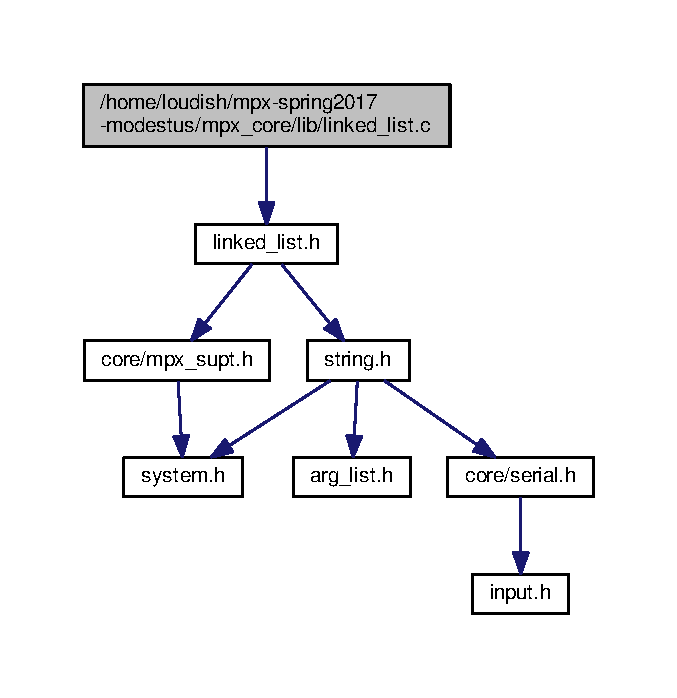
\includegraphics[width=325pt]{linked__list_8c__incl}
\end{center}
\end{figure}
\subsection*{Functions}
\begin{DoxyCompactItemize}
\item 
void \hyperlink{linked__list_8c_a88e42961d952fbe5abb7e8cb26c916cc}{init\+Linked\+List} (\hyperlink{structlinked_list__t}{linked\+List\+\_\+t} $\ast$list)
\begin{DoxyCompactList}\small\item\em initilize list and the optional array that backs the list \end{DoxyCompactList}\item 
\hyperlink{structnode__t}{node\+\_\+t} $\ast$ \hyperlink{linked__list_8c_a042e8aa38eb81453dd7e81ade7d38b5b}{make\+New\+Node} (\hyperlink{structlinked_list__t}{linked\+List\+\_\+t} $\ast$list, void $\ast$data)
\begin{DoxyCompactList}\small\item\em get new node, allocate a new node or find an unused node from the list\textquotesingle{}s pool \end{DoxyCompactList}\item 
void \hyperlink{linked__list_8c_a45d030386936adffa3eb5586ce93d131}{set\+Insert\+Comparison\+Function} (\hyperlink{structlinked_list__t}{linked\+List\+\_\+t} $\ast$list, int($\ast$new\+Comp\+Func)(void $\ast$, void $\ast$))
\begin{DoxyCompactList}\small\item\em takes in a function pointer and sets the library shared comparison pointer \end{DoxyCompactList}\item 
void \hyperlink{linked__list_8c_a3b6f817f74d12d2cf4a35405f447c73d}{set\+Free\+Function} (\hyperlink{structlinked_list__t}{linked\+List\+\_\+t} $\ast$list, int($\ast$new\+Free\+Func)(\hyperlink{structnode__t}{node\+\_\+t} $\ast$))
\begin{DoxyCompactList}\small\item\em sets the function whose job it is to free the node\textquotesingle{}s memory \end{DoxyCompactList}\item 
void \hyperlink{linked__list_8c_a12e5138ac02af0f6b42ff2f1b29c610a}{set\+Search\+Comparison\+Function} (\hyperlink{structlinked_list__t}{linked\+List\+\_\+t} $\ast$list, int($\ast$new\+Search\+Func)(void $\ast$, void $\ast$))
\begin{DoxyCompactList}\small\item\em sets the function whose job it is to compare the input data with the data in the list. the first void parameter will always be the data contained in the list, the second will be the data passed to the search function. \end{DoxyCompactList}\item 
\hyperlink{structnode__t}{node\+\_\+t} $\ast$ \hyperlink{linked__list_8c_a20871a48a5ca68065f74200de139228b}{insert\+After\+Node} (\hyperlink{structnode__t}{node\+\_\+t} $\ast$preceeding\+Node, \hyperlink{structnode__t}{node\+\_\+t} $\ast$new\+Node)
\begin{DoxyCompactList}\small\item\em insert a node into the parent list of the preceeding\+Node after preceeding\+Node \end{DoxyCompactList}\item 
\hyperlink{structnode__t}{node\+\_\+t} $\ast$ \hyperlink{linked__list_8c_a04df23f8eb8508551930249bad9f159a}{insert\+Before\+Node} (\hyperlink{structnode__t}{node\+\_\+t} $\ast$node\+To\+Follow, \hyperlink{structnode__t}{node\+\_\+t} $\ast$new\+Node)
\begin{DoxyCompactList}\small\item\em insert a node into the parent list of the node\+To\+Follow before node\+To\+Follow \end{DoxyCompactList}\item 
\hyperlink{structnode__t}{node\+\_\+t} $\ast$ \hyperlink{linked__list_8c_ad225d0f3d9e1b59a58117ba0bc491189}{remove\+Node} (\hyperlink{structnode__t}{node\+\_\+t} $\ast$node\+To\+Remove)
\begin{DoxyCompactList}\small\item\em will remove the node from the list. the list hierarchy will change to reflect the missing node. \end{DoxyCompactList}\item 
\hyperlink{structnode__t}{node\+\_\+t} $\ast$ \hyperlink{linked__list_8c_a1573ed6fa569b80577b596e78cd90b4a}{move\+Node\+To\+New\+List} (\hyperlink{structnode__t}{node\+\_\+t} $\ast$node\+To\+Move, \hyperlink{structlinked_list__t}{linked\+List\+\_\+t} $\ast$new\+List)
\begin{DoxyCompactList}\small\item\em If a node needs to move lists and lists are array backed, instead of just moving preceeding and suceeding pointers of the node, the node actaully needs to move backing arrays so one list\textquotesingle{}s nodes are not the only ones being consumed. The equivalent process will be to execute the parent list\textquotesingle{}s remove\+Node funcion, execute the make\+New\+Node function on the new\+List, copy all structure members to the new node, and return the new node. The list of node\+To\+Move free\+Node\+Func will be called with node\+To\+Mov as the argument. If the lists are not array backed, the function simply removes the node from its containing list and calls insert\+Node on the new list. \end{DoxyCompactList}\item 
\hyperlink{structnode__t}{node\+\_\+t} $\ast$ \hyperlink{linked__list_8c_a75ff37d4b2282fa64cb59415e17f8ee5}{search\+List} (\hyperlink{structlinked_list__t}{linked\+List\+\_\+t} $\ast$list\+To\+Search, void $\ast$data)
\begin{DoxyCompactList}\small\item\em goes through the list using the list\textquotesingle{}s comparison function to find the node which matches the data. if the search function is undefined for this list, the function returns null immedietly. \end{DoxyCompactList}\item 
\hyperlink{structnode__t}{node\+\_\+t} $\ast$ \hyperlink{linked__list_8c_a40b9cae4db9ce33443e541191e75f540}{insert\+Node} (\hyperlink{structlinked_list__t}{linked\+List\+\_\+t} $\ast$list, \hyperlink{structnode__t}{node\+\_\+t} $\ast$new\+Node)
\begin{DoxyCompactList}\small\item\em Will insert the node into the list. This function will attempt to call the list\textquotesingle{}s \hyperlink{linked__list_8c_a45d030386936adffa3eb5586ce93d131}{insert comparison} function if defined. The function will insert the new node into the list after this function returns $>$ 0. If the \hyperlink{linked__list_8c_a45d030386936adffa3eb5586ce93d131}{insert comparison} function is not defined for this list, the inserting function will placed the new node at the end of the list before the tail. \end{DoxyCompactList}\item 
void \hyperlink{group___r2_gafc8969d7969f61c928a01f4c302e669b}{set\+Print\+Function} (\hyperlink{structlinked_list__t}{linked\+List\+\_\+t} $\ast$list, void($\ast$new\+Print\+Func)(void $\ast$))
\begin{DoxyCompactList}\small\item\em sets the function whose job it is to print the list to the screen. \end{DoxyCompactList}\item 
void \hyperlink{linked__list_8c_a9bbec3837a303ae4bbc5eafb23ead2d5}{print\+List} (\hyperlink{structlinked_list__t}{linked\+List\+\_\+t} $\ast$list)
\begin{DoxyCompactList}\small\item\em test function to show list functionality. uses const char$\ast$ as test data \end{DoxyCompactList}\item 
int \hyperlink{linked__list_8c_aa034eb9ccc5e7790304204b1cb0ed60f}{comp\+Function} (void $\ast$node\+Data1, void $\ast$node\+Data2)
\item 
int \hyperlink{linked__list_8c_aec835b94f0f2d661880b5e2f75cefada}{searchcomp\+Function} (void $\ast$node\+Data1, void $\ast$node\+Data2)
\item 
void \hyperlink{linked__list_8c_abce3e0a671a927747db173dea67b2afc}{test\+Print\+Func} (void $\ast$node\+Data)
\item 
void \hyperlink{linked__list_8c_a0a60ac1fe6e5055de61277ac9703b13e}{list\+Test} ()
\begin{DoxyCompactList}\small\item\em test the linked\+\_\+list class with const char$\ast$ data and output to screen the results of the test \end{DoxyCompactList}\end{DoxyCompactItemize}


\subsection{Function Documentation}
\index{linked\+\_\+list.\+c@{linked\+\_\+list.\+c}!comp\+Function@{comp\+Function}}
\index{comp\+Function@{comp\+Function}!linked\+\_\+list.\+c@{linked\+\_\+list.\+c}}
\subsubsection[{\texorpdfstring{comp\+Function(void $\ast$node\+Data1, void $\ast$node\+Data2)}{compFunction(void *nodeData1, void *nodeData2)}}]{\setlength{\rightskip}{0pt plus 5cm}int comp\+Function (
\begin{DoxyParamCaption}
\item[{void $\ast$}]{node\+Data1, }
\item[{void $\ast$}]{node\+Data2}
\end{DoxyParamCaption}
)}\hypertarget{linked__list_8c_aa034eb9ccc5e7790304204b1cb0ed60f}{}\label{linked__list_8c_aa034eb9ccc5e7790304204b1cb0ed60f}


Definition at line 230 of file linked\+\_\+list.\+c.



Referenced by list\+Test().


\begin{DoxyCode}
231 \{
232     \textcolor{comment}{//return strcmp((const char*)(nodeData1), (const char*)(nodeData2));}
233     (void)nodeData1; (void)nodeData2;
234     \textcolor{keywordflow}{return} -1;
235 \}
\end{DoxyCode}
\index{linked\+\_\+list.\+c@{linked\+\_\+list.\+c}!init\+Linked\+List@{init\+Linked\+List}}
\index{init\+Linked\+List@{init\+Linked\+List}!linked\+\_\+list.\+c@{linked\+\_\+list.\+c}}
\subsubsection[{\texorpdfstring{init\+Linked\+List(linked\+List\+\_\+t $\ast$list)}{initLinkedList(linkedList_t *list)}}]{\setlength{\rightskip}{0pt plus 5cm}void init\+Linked\+List (
\begin{DoxyParamCaption}
\item[{{\bf linked\+List\+\_\+t} $\ast$}]{list}
\end{DoxyParamCaption}
)}\hypertarget{linked__list_8c_a88e42961d952fbe5abb7e8cb26c916cc}{}\label{linked__list_8c_a88e42961d952fbe5abb7e8cb26c916cc}


initilize list and the optional array that backs the list 


\begin{DoxyParams}{Parameters}
{\em list} & pointer to list \\
\hline
\end{DoxyParams}


Definition at line 3 of file linked\+\_\+list.\+c.



References M\+A\+X\+\_\+\+N\+U\+M\+\_\+\+O\+F\+\_\+\+L\+L\+\_\+\+N\+O\+D\+ES.



Referenced by init\+P\+C\+B\+Queues(), and list\+Test().


\begin{DoxyCode}
4 \{
5 \textcolor{preprocessor}{#ifdef LL\_IS\_ARRAY\_BACKED}
6     \textcolor{keywordtype}{int} i;
7     \textcolor{keywordflow}{for}(i=0; i < \hyperlink{linked__list_8h_a4bdabb4388c831c1f8c4d31e67801e74}{MAX\_NUM\_OF\_LL\_NODES}; i++)
8     \{
9         list->backingArray[i].data=0;
10         list->backingArray[i].inUse=0;
11         list->backingArray[i].next=0;
12         list->backingArray[i].prev=0;
13         list->backingArray[i].parentList = list;
14     \}
15 
16     list->head.parentList = list;
17     list->head.inUse=1;
18 
19     list->tail.parentList = list;
20     list->tail.inUse=1;
21 \textcolor{preprocessor}{#endif}
22 
23     list->head.data=0;
24     list->head.next =
25         list->head.prev = &list->tail;
26 
27     list->tail.data=0;
28     list->tail.next =
29         list->tail.prev = &list->head;
30 
31     list->length = 0;
32     list->insertCompFunc = 0;
33     list->freeNodeFunc = 0;
34     list->searchCompFunc = 0;
35 \}
\end{DoxyCode}
\index{linked\+\_\+list.\+c@{linked\+\_\+list.\+c}!insert\+After\+Node@{insert\+After\+Node}}
\index{insert\+After\+Node@{insert\+After\+Node}!linked\+\_\+list.\+c@{linked\+\_\+list.\+c}}
\subsubsection[{\texorpdfstring{insert\+After\+Node(node\+\_\+t $\ast$preceeding\+Node, node\+\_\+t $\ast$new\+Node)}{insertAfterNode(node_t *preceedingNode, node_t *newNode)}}]{\setlength{\rightskip}{0pt plus 5cm}{\bf node\+\_\+t}$\ast$ insert\+After\+Node (
\begin{DoxyParamCaption}
\item[{{\bf node\+\_\+t} $\ast$}]{preceeding\+Node, }
\item[{{\bf node\+\_\+t} $\ast$}]{new\+Node}
\end{DoxyParamCaption}
)}\hypertarget{linked__list_8c_a20871a48a5ca68065f74200de139228b}{}\label{linked__list_8c_a20871a48a5ca68065f74200de139228b}


insert a node into the parent list of the preceeding\+Node after preceeding\+Node 


\begin{DoxyParams}{Parameters}
{\em preceeding\+Node} & node to insert the new node afterwards \\
\hline
{\em new\+Node} & the new node to insert. if the list is array backed, the new\+Node will be copied to the list\textquotesingle{}s node pool if it currently does not reside there \\
\hline
\end{DoxyParams}
\begin{DoxyReturn}{Returns}
pointer to node inserted in the parent list of preceeding\+Node, null if insertion failed 
\end{DoxyReturn}


Definition at line 78 of file linked\+\_\+list.\+c.



References move\+Node\+To\+New\+List().


\begin{DoxyCode}
79 \{
80 \textcolor{preprocessor}{#ifdef LL\_IS\_ARRAY\_BACKED}
81     \textcolor{keywordflow}{if}(preceedingNode->parentList != newNode->parentList)
82     \{
83         \textcolor{comment}{//if the node to insert is not apart of the list to insert after, the function moveNodeToNewList
       makes a}
84             \textcolor{comment}{//new node in the parent list of the preceedingNode and recursively calls this function with
       the newly moved node}
85         \textcolor{keywordflow}{return} \hyperlink{linked__list_8c_a20871a48a5ca68065f74200de139228b}{insertAfterNode}(preceedingNode,
86                             \hyperlink{linked__list_8c_a1573ed6fa569b80577b596e78cd90b4a}{moveNodeToNewList}(newNode, preceedingNode->parentList));
87     \}
88 \textcolor{preprocessor}{#endif}
89 
90     newNode->next = preceedingNode->next;
91     newNode->prev = preceedingNode;
92 
93     newNode->next->prev = newNode;
94     newNode->prev->next = newNode;
95 
96     \textcolor{keywordflow}{return} newNode;
97 \}
\end{DoxyCode}
\index{linked\+\_\+list.\+c@{linked\+\_\+list.\+c}!insert\+Before\+Node@{insert\+Before\+Node}}
\index{insert\+Before\+Node@{insert\+Before\+Node}!linked\+\_\+list.\+c@{linked\+\_\+list.\+c}}
\subsubsection[{\texorpdfstring{insert\+Before\+Node(node\+\_\+t $\ast$node\+To\+Follow, node\+\_\+t $\ast$new\+Node)}{insertBeforeNode(node_t *nodeToFollow, node_t *newNode)}}]{\setlength{\rightskip}{0pt plus 5cm}{\bf node\+\_\+t}$\ast$ insert\+Before\+Node (
\begin{DoxyParamCaption}
\item[{{\bf node\+\_\+t} $\ast$}]{node\+To\+Follow, }
\item[{{\bf node\+\_\+t} $\ast$}]{new\+Node}
\end{DoxyParamCaption}
)}\hypertarget{linked__list_8c_a04df23f8eb8508551930249bad9f159a}{}\label{linked__list_8c_a04df23f8eb8508551930249bad9f159a}


insert a node into the parent list of the node\+To\+Follow before node\+To\+Follow 


\begin{DoxyParams}{Parameters}
{\em node\+To\+Follow} & node to insert the new\+Node before \\
\hline
{\em new\+Node} & the new node to insert. if the list is array backed, the new\+Node will be copied to the list\textquotesingle{}s node pool if it currently does not reside there \\
\hline
\end{DoxyParams}
\begin{DoxyReturn}{Returns}
pointer to node inserted in the parent list of node\+To\+Follow, null if insertion failed 
\end{DoxyReturn}


Definition at line 99 of file linked\+\_\+list.\+c.



References move\+Node\+To\+New\+List().



Referenced by insert\+Node().


\begin{DoxyCode}
100 \{
101 \textcolor{preprocessor}{#ifdef LL\_IS\_ARRAY\_BACKED}
102     \textcolor{keywordflow}{if}(nodeToFollow->parentList != newNode->parentList)
103     \{
104         \textcolor{comment}{//if the node to insert is not apart of the list to insert after, the function moveNodeToNewList
       makes a}
105             \textcolor{comment}{//new node in the parent list of the preceedingNode and recursively calls this function with
       the newly moved node}
106         \textcolor{keywordflow}{return} \hyperlink{linked__list_8c_a04df23f8eb8508551930249bad9f159a}{insertBeforeNode}(nodeToFollow,
107                             \hyperlink{linked__list_8c_a1573ed6fa569b80577b596e78cd90b4a}{moveNodeToNewList}(newNode, nodeToFollow->parentList));
108     \}
109 \textcolor{preprocessor}{#endif}
110 
111     newNode->next = nodeToFollow;
112     newNode->prev = nodeToFollow->prev;
113 
114     newNode->next->prev = newNode;
115     newNode->prev->next = newNode;
116 
117     \textcolor{keywordflow}{return} newNode;
118 \}
\end{DoxyCode}
\index{linked\+\_\+list.\+c@{linked\+\_\+list.\+c}!insert\+Node@{insert\+Node}}
\index{insert\+Node@{insert\+Node}!linked\+\_\+list.\+c@{linked\+\_\+list.\+c}}
\subsubsection[{\texorpdfstring{insert\+Node(linked\+List\+\_\+t $\ast$list, node\+\_\+t $\ast$new\+Node)}{insertNode(linkedList_t *list, node_t *newNode)}}]{\setlength{\rightskip}{0pt plus 5cm}{\bf node\+\_\+t}$\ast$ insert\+Node (
\begin{DoxyParamCaption}
\item[{{\bf linked\+List\+\_\+t} $\ast$}]{list, }
\item[{{\bf node\+\_\+t} $\ast$}]{new\+Node}
\end{DoxyParamCaption}
)}\hypertarget{linked__list_8c_a40b9cae4db9ce33443e541191e75f540}{}\label{linked__list_8c_a40b9cae4db9ce33443e541191e75f540}


Will insert the node into the list. This function will attempt to call the list\textquotesingle{}s \hyperlink{linked__list_8c_a45d030386936adffa3eb5586ce93d131}{insert comparison} function if defined. The function will insert the new node into the list after this function returns $>$ 0. If the \hyperlink{linked__list_8c_a45d030386936adffa3eb5586ce93d131}{insert comparison} function is not defined for this list, the inserting function will placed the new node at the end of the list before the tail. 


\begin{DoxyParams}{Parameters}
{\em list} & list to place the node \\
\hline
{\em new\+Node} & the new node to insert. if the list is array backed, the new\+Node will be copied to the list\textquotesingle{}s node pool if it currently does not reside there \\
\hline
\end{DoxyParams}
\begin{DoxyReturn}{Returns}
pointer to the node in the new list, or null if inserting failed. 
\end{DoxyReturn}


Definition at line 173 of file linked\+\_\+list.\+c.



References insert\+Before\+Node(), and move\+Node\+To\+New\+List().



Referenced by insert\+P\+C\+B(), list\+Test(), move\+Node\+To\+New\+List(), and setup\+P\+C\+B().


\begin{DoxyCode}
174 \{
175     \textcolor{comment}{//if newNode is not valid, do not insert any node}
176     \textcolor{keywordflow}{if}(!newNode)
177     \{
178         \textcolor{keywordflow}{return} 0;
179     \}
180 
181 \textcolor{preprocessor}{#ifdef LL\_IS\_ARRAY\_BACKED}
182     \textcolor{keywordflow}{if}(newNode->parentList != list)
183     \{
184         \textcolor{comment}{//if the node to insert is not apart of the list to insert after, the function moveNodeToNewList
       makes a}
185             \textcolor{comment}{//new node in the parent list of the preceedingNode and recursively calls this function with
       the newly moved node}
186         \textcolor{keywordflow}{return} \hyperlink{linked__list_8c_a40b9cae4db9ce33443e541191e75f540}{insertNode}(list, \hyperlink{linked__list_8c_a1573ed6fa569b80577b596e78cd90b4a}{moveNodeToNewList}(newNode, list));
187     \}
188 \textcolor{preprocessor}{#endif}
189 
190     \textcolor{keywordflow}{if}(list->insertCompFunc)
191     \{
192         \hyperlink{structnode__t}{node\_t} * itNode = list->head.next;
193         \textcolor{keywordflow}{for}(; itNode != &(list->tail); itNode = itNode->next)
194         \{
195             \textcolor{keywordtype}{int} result = ((*(list->insertCompFunc))(itNode->data, newNode->data));
196             \textcolor{keywordflow}{if}(result > 0)
197             \{
198                 list->length++;
199                 \textcolor{keywordflow}{return} \hyperlink{linked__list_8c_a04df23f8eb8508551930249bad9f159a}{insertBeforeNode}(itNode, newNode);
200             \}
201         \}
202     \}
203     \textcolor{keywordflow}{return} \hyperlink{linked__list_8c_a04df23f8eb8508551930249bad9f159a}{insertBeforeNode}(&(list->tail), newNode);
204 \}
\end{DoxyCode}
\index{linked\+\_\+list.\+c@{linked\+\_\+list.\+c}!list\+Test@{list\+Test}}
\index{list\+Test@{list\+Test}!linked\+\_\+list.\+c@{linked\+\_\+list.\+c}}
\subsubsection[{\texorpdfstring{list\+Test()}{listTest()}}]{\setlength{\rightskip}{0pt plus 5cm}void list\+Test (
\begin{DoxyParamCaption}
{}
\end{DoxyParamCaption}
)}\hypertarget{linked__list_8c_a0a60ac1fe6e5055de61277ac9703b13e}{}\label{linked__list_8c_a0a60ac1fe6e5055de61277ac9703b13e}


test the linked\+\_\+list class with const char$\ast$ data and output to screen the results of the test 



Definition at line 249 of file linked\+\_\+list.\+c.



References comp\+Function(), init\+Linked\+List(), insert\+Node(), make\+New\+Node(), printf, print\+List(), searchcomp\+Function(), search\+List(), set\+Insert\+Comparison\+Function(), set\+Print\+Function(), set\+Search\+Comparison\+Function(), and test\+Print\+Func().



Referenced by kmain().


\begin{DoxyCode}
250 \{
251     \hyperlink{structlinked_list__t}{linkedList\_t} list1;
252     \hyperlink{structlinked_list__t}{linkedList\_t} list2;
253 
254     \hyperlink{linked__list_8c_a88e42961d952fbe5abb7e8cb26c916cc}{initLinkedList}(&list1);
255     \hyperlink{linked__list_8c_a88e42961d952fbe5abb7e8cb26c916cc}{initLinkedList}(&list2);
256 
257     \hyperlink{linked__list_8c_a45d030386936adffa3eb5586ce93d131}{setInsertComparisonFunction}(&list1, &\hyperlink{linked__list_8c_aa034eb9ccc5e7790304204b1cb0ed60f}{compFunction});
258     \hyperlink{linked__list_8c_a12e5138ac02af0f6b42ff2f1b29c610a}{setSearchComparisonFunction}(&list1, &
      \hyperlink{linked__list_8c_aec835b94f0f2d661880b5e2f75cefada}{searchcompFunction});
259     \hyperlink{group___r2_gafc8969d7969f61c928a01f4c302e669b}{setPrintFunction}(&list1, &\hyperlink{linked__list_8c_abce3e0a671a927747db173dea67b2afc}{testPrintFunc});
260 
261     \hyperlink{linked__list_8c_a40b9cae4db9ce33443e541191e75f540}{insertNode}(&list1, \hyperlink{linked__list_8c_a042e8aa38eb81453dd7e81ade7d38b5b}{makeNewNode}(&list2, (\textcolor{keywordtype}{void}*)\textcolor{stringliteral}{"test3"}));
262     \hyperlink{linked__list_8c_a40b9cae4db9ce33443e541191e75f540}{insertNode}(&list1, \hyperlink{linked__list_8c_a042e8aa38eb81453dd7e81ade7d38b5b}{makeNewNode}(&list2, (\textcolor{keywordtype}{void}*)\textcolor{stringliteral}{"test1"}));
263     \hyperlink{linked__list_8c_a40b9cae4db9ce33443e541191e75f540}{insertNode}(&list1, \hyperlink{linked__list_8c_a042e8aa38eb81453dd7e81ade7d38b5b}{makeNewNode}(&list2, (\textcolor{keywordtype}{void}*)\textcolor{stringliteral}{"test5"}));
264     \hyperlink{linked__list_8c_a40b9cae4db9ce33443e541191e75f540}{insertNode}(&list1, \hyperlink{linked__list_8c_a042e8aa38eb81453dd7e81ade7d38b5b}{makeNewNode}(&list2, (\textcolor{keywordtype}{void}*)\textcolor{stringliteral}{"test2"}));
265     \hyperlink{linked__list_8c_a40b9cae4db9ce33443e541191e75f540}{insertNode}(&list1, \hyperlink{linked__list_8c_a042e8aa38eb81453dd7e81ade7d38b5b}{makeNewNode}(&list2, (\textcolor{keywordtype}{void}*)\textcolor{stringliteral}{"test7"}));
266     \hyperlink{linked__list_8c_a40b9cae4db9ce33443e541191e75f540}{insertNode}(&list1, \hyperlink{linked__list_8c_a042e8aa38eb81453dd7e81ade7d38b5b}{makeNewNode}(&list2, (\textcolor{keywordtype}{void}*)\textcolor{stringliteral}{"test4"}));
267     \hyperlink{linked__list_8c_a40b9cae4db9ce33443e541191e75f540}{insertNode}(&list1, \hyperlink{linked__list_8c_a042e8aa38eb81453dd7e81ade7d38b5b}{makeNewNode}(&list2, (\textcolor{keywordtype}{void}*)\textcolor{stringliteral}{"test8"}));
268     \hyperlink{linked__list_8c_a40b9cae4db9ce33443e541191e75f540}{insertNode}(&list1, \hyperlink{linked__list_8c_a042e8aa38eb81453dd7e81ade7d38b5b}{makeNewNode}(&list2, (\textcolor{keywordtype}{void}*)\textcolor{stringliteral}{"test3"}));
269 
270 
271    \textcolor{comment}{// node\_t * nodeFound = searchList(&list1, (void*)"test3");}
272 
273     \hyperlink{structnode__t}{node\_t} * nodeFound = \hyperlink{linked__list_8c_a75ff37d4b2282fa64cb59415e17f8ee5}{searchList}(&list1, (\textcolor{keywordtype}{void}*)\textcolor{stringliteral}{"test5"});
274     \hyperlink{string_8h_a0f459d16901ef591acaafa4b67fd4be5}{printf}(\textcolor{stringliteral}{"looking for node whose data is: %s\(\backslash\)r\(\backslash\)nsearch return: %d\(\backslash\)r\(\backslash\)n"}, \textcolor{stringliteral}{"test5"}, (\textcolor{keywordtype}{int})nodeFound);
275 
276     \textcolor{keywordflow}{if}(nodeFound)
277     \{
278         \hyperlink{string_8h_a0f459d16901ef591acaafa4b67fd4be5}{printf}(\textcolor{stringliteral}{"found node:: data string = %s\(\backslash\)r\(\backslash\)n"}, (\textcolor{keyword}{const} \textcolor{keywordtype}{char}*)nodeFound->data);
279     \}
280 
281     \hyperlink{linked__list_8c_a9bbec3837a303ae4bbc5eafb23ead2d5}{printList}(&list1);
282 \}
\end{DoxyCode}
\index{linked\+\_\+list.\+c@{linked\+\_\+list.\+c}!make\+New\+Node@{make\+New\+Node}}
\index{make\+New\+Node@{make\+New\+Node}!linked\+\_\+list.\+c@{linked\+\_\+list.\+c}}
\subsubsection[{\texorpdfstring{make\+New\+Node(linked\+List\+\_\+t $\ast$list, void $\ast$data)}{makeNewNode(linkedList_t *list, void *data)}}]{\setlength{\rightskip}{0pt plus 5cm}{\bf node\+\_\+t}$\ast$ make\+New\+Node (
\begin{DoxyParamCaption}
\item[{{\bf linked\+List\+\_\+t} $\ast$}]{list, }
\item[{void $\ast$}]{data}
\end{DoxyParamCaption}
)}\hypertarget{linked__list_8c_a042e8aa38eb81453dd7e81ade7d38b5b}{}\label{linked__list_8c_a042e8aa38eb81453dd7e81ade7d38b5b}


get new node, allocate a new node or find an unused node from the list\textquotesingle{}s pool 


\begin{DoxyParams}{Parameters}
{\em list} & to find an unused node from. This argument is ignored if the list is dynamically allocated \\
\hline
{\em data} & pointer to the data the new node should contain, the pointer must be valid obviously \\
\hline
\end{DoxyParams}
\begin{DoxyReturn}{Returns}
pointer to new node, null if no new node could be found or created 
\end{DoxyReturn}


Definition at line 37 of file linked\+\_\+list.\+c.



References M\+A\+X\+\_\+\+N\+U\+M\+\_\+\+O\+F\+\_\+\+L\+L\+\_\+\+N\+O\+D\+ES, and sys\+\_\+alloc\+\_\+mem().



Referenced by allocate\+P\+C\+B(), list\+Test(), and move\+Node\+To\+New\+List().


\begin{DoxyCode}
38 \{
39 \textcolor{preprocessor}{#ifdef LL\_IS\_ARRAY\_BACKED}
40     \textcolor{keywordtype}{int} i;
41     \textcolor{keywordflow}{for}(i=0; i < \hyperlink{linked__list_8h_a4bdabb4388c831c1f8c4d31e67801e74}{MAX\_NUM\_OF\_LL\_NODES}; i++)
42     \{
43         \textcolor{keywordflow}{if}(!list->backingArray[i].inUse)
44         \{
45             list->backingArray[i].inUse = 1;
46             list->numNodesInUse++;
47             list->backingArray[i].data = data;
48             \textcolor{keywordflow}{return} &(list->backingArray[i]);
49         \}
50     \}
51     \textcolor{keywordflow}{return} 0;
52 \textcolor{preprocessor}{#else}
53     (void)list;
54     \hyperlink{structnode__t}{node\_t} * newNode = \hyperlink{include_2core_2mpx__supt_8h_a61adad2abba0a3a225c2290b3de1fe93}{sys\_alloc\_mem}(\textcolor{keyword}{sizeof}(\hyperlink{structnode__t}{node\_t}));
55     newNode->data = data;
56     newNode->next=0;
57     newNode->prev=0;
58     \textcolor{keywordflow}{return} newNode;
59 
60 \textcolor{preprocessor}{#endif}
61 \}
\end{DoxyCode}
\index{linked\+\_\+list.\+c@{linked\+\_\+list.\+c}!move\+Node\+To\+New\+List@{move\+Node\+To\+New\+List}}
\index{move\+Node\+To\+New\+List@{move\+Node\+To\+New\+List}!linked\+\_\+list.\+c@{linked\+\_\+list.\+c}}
\subsubsection[{\texorpdfstring{move\+Node\+To\+New\+List(node\+\_\+t $\ast$node\+To\+Move, linked\+List\+\_\+t $\ast$new\+List)}{moveNodeToNewList(node_t *nodeToMove, linkedList_t *newList)}}]{\setlength{\rightskip}{0pt plus 5cm}{\bf node\+\_\+t}$\ast$ move\+Node\+To\+New\+List (
\begin{DoxyParamCaption}
\item[{{\bf node\+\_\+t} $\ast$}]{node\+To\+Move, }
\item[{{\bf linked\+List\+\_\+t} $\ast$}]{new\+List}
\end{DoxyParamCaption}
)}\hypertarget{linked__list_8c_a1573ed6fa569b80577b596e78cd90b4a}{}\label{linked__list_8c_a1573ed6fa569b80577b596e78cd90b4a}


If a node needs to move lists and lists are array backed, instead of just moving preceeding and suceeding pointers of the node, the node actaully needs to move backing arrays so one list\textquotesingle{}s nodes are not the only ones being consumed. The equivalent process will be to execute the parent list\textquotesingle{}s remove\+Node funcion, execute the make\+New\+Node function on the new\+List, copy all structure members to the new node, and return the new node. The list of node\+To\+Move free\+Node\+Func will be called with node\+To\+Mov as the argument. If the lists are not array backed, the function simply removes the node from its containing list and calls insert\+Node on the new list. 


\begin{DoxyParams}{Parameters}
{\em node\+To\+Move} & the node to move, this pointer is no longer guarenteed to be valid. Stop using this pointer, \\
\hline
{\em new\+List} & the list to move the node to, this will be the node\textquotesingle{}s new parent list \\
\hline
\end{DoxyParams}
\begin{DoxyReturn}{Returns}
the pointer of param node\+To\+Move will no longer be valid, the pointer to the node in the new list will be returned on sucess. Null on failure and node\+To\+Move will remain valid 
\end{DoxyReturn}


Definition at line 132 of file linked\+\_\+list.\+c.



References insert\+Node(), make\+New\+Node(), and remove\+Node().



Referenced by insert\+After\+Node(), insert\+Before\+Node(), and insert\+Node().


\begin{DoxyCode}
133 \{
134 \textcolor{preprocessor}{#ifdef LL\_IS\_ARRAY\_BACKED}
135     \hyperlink{structnode__t}{node\_t} *  newNodeInList = \hyperlink{linked__list_8c_a042e8aa38eb81453dd7e81ade7d38b5b}{makeNewNode}(newList, nodeToMove->data);
136     \textcolor{keywordflow}{if}(!newNodeInList)
137     \{
138         \textcolor{keywordflow}{return} 0;
139     \}
140 
141     \hyperlink{linked__list_8c_ad225d0f3d9e1b59a58117ba0bc491189}{removeNode}(nodeToMove);
142 
143     \textcolor{keywordflow}{if}(nodeToMove->parentList->freeNodeFunc)
144     \{
145         (*(nodeToMove->parentList->freeNodeFunc))(nodeToMove);
146     \}
147     \textcolor{keywordflow}{return} newNodeInList;
148 \textcolor{preprocessor}{#else}
149     \hyperlink{structnode__t}{node\_t}* removedNode = \hyperlink{linked__list_8c_ad225d0f3d9e1b59a58117ba0bc491189}{removeNode}(nodeToMove);
150     \textcolor{keywordflow}{return} \hyperlink{linked__list_8c_a40b9cae4db9ce33443e541191e75f540}{insertNode}(newList, removedNode);
151 \textcolor{preprocessor}{#endif}
152 \}
\end{DoxyCode}
\index{linked\+\_\+list.\+c@{linked\+\_\+list.\+c}!print\+List@{print\+List}}
\index{print\+List@{print\+List}!linked\+\_\+list.\+c@{linked\+\_\+list.\+c}}
\subsubsection[{\texorpdfstring{print\+List(linked\+List\+\_\+t $\ast$list)}{printList(linkedList_t *list)}}]{\setlength{\rightskip}{0pt plus 5cm}void print\+List (
\begin{DoxyParamCaption}
\item[{{\bf linked\+List\+\_\+t} $\ast$}]{list}
\end{DoxyParamCaption}
)}\hypertarget{linked__list_8c_a9bbec3837a303ae4bbc5eafb23ead2d5}{}\label{linked__list_8c_a9bbec3837a303ae4bbc5eafb23ead2d5}


test function to show list functionality. uses const char$\ast$ as test data 


\begin{DoxyParams}{Parameters}
{\em list} & list to print the nodes of \\
\hline
\end{DoxyParams}


Definition at line 211 of file linked\+\_\+list.\+c.



References printf.



Referenced by list\+Test(), pcb\+Test(), show\+All\+Processes(), show\+Blocked\+Processes(), and show\+Ready\+Processes().


\begin{DoxyCode}
212 \{
213     \textcolor{keywordflow}{if}(list->printNodeFunc)
214     \{
215         \hyperlink{structnode__t}{node\_t} * itNode = list->head.next;
216         \textcolor{keywordflow}{if}(itNode == &(list->tail))
217         \{
218             \hyperlink{string_8h_a0f459d16901ef591acaafa4b67fd4be5}{printf}(\textcolor{stringliteral}{"%s"},\textcolor{stringliteral}{"<List is Empty>\(\backslash\)r\(\backslash\)n"});
219         \}
220         \textcolor{keywordflow}{for}(; itNode != &(list->tail); itNode = itNode->next)
221         \{
222             list->printNodeFunc(itNode->data);
223         \}
224     \}\textcolor{keywordflow}{else}
225     \{
226         \hyperlink{string_8h_a0f459d16901ef591acaafa4b67fd4be5}{printf}(\textcolor{stringliteral}{"No Search Function provided for List!%s\(\backslash\)r\(\backslash\)n"},\textcolor{stringliteral}{" "});
227     \}
228 \}
\end{DoxyCode}
\index{linked\+\_\+list.\+c@{linked\+\_\+list.\+c}!remove\+Node@{remove\+Node}}
\index{remove\+Node@{remove\+Node}!linked\+\_\+list.\+c@{linked\+\_\+list.\+c}}
\subsubsection[{\texorpdfstring{remove\+Node(node\+\_\+t $\ast$node\+To\+Remove)}{removeNode(node_t *nodeToRemove)}}]{\setlength{\rightskip}{0pt plus 5cm}{\bf node\+\_\+t}$\ast$ remove\+Node (
\begin{DoxyParamCaption}
\item[{{\bf node\+\_\+t} $\ast$}]{node\+To\+Remove}
\end{DoxyParamCaption}
)}\hypertarget{linked__list_8c_ad225d0f3d9e1b59a58117ba0bc491189}{}\label{linked__list_8c_ad225d0f3d9e1b59a58117ba0bc491189}


will remove the node from the list. the list hierarchy will change to reflect the missing node. 


\begin{DoxyParams}{Parameters}
{\em node\+To\+Remove} & pointer to the node to remove \\
\hline
\end{DoxyParams}
\begin{DoxyReturn}{Returns}
pointer to the removed node 
\end{DoxyReturn}


Definition at line 120 of file linked\+\_\+list.\+c.



Referenced by move\+Node\+To\+New\+List(), and remove\+P\+C\+B().


\begin{DoxyCode}
121 \{
122     \textcolor{keywordflow}{if}(nodeToRemove)
123     \{
124         \textcolor{keywordflow}{if}(nodeToRemove->prev)\{nodeToRemove->prev->next = nodeToRemove->next;\}
125         \textcolor{keywordflow}{if}(nodeToRemove->next)\{nodeToRemove->next->prev = nodeToRemove->prev;\}
126         nodeToRemove->next = 0;
127         nodeToRemove->prev = 0;
128     \}
129     \textcolor{keywordflow}{return} nodeToRemove;
130 \}
\end{DoxyCode}
\index{linked\+\_\+list.\+c@{linked\+\_\+list.\+c}!searchcomp\+Function@{searchcomp\+Function}}
\index{searchcomp\+Function@{searchcomp\+Function}!linked\+\_\+list.\+c@{linked\+\_\+list.\+c}}
\subsubsection[{\texorpdfstring{searchcomp\+Function(void $\ast$node\+Data1, void $\ast$node\+Data2)}{searchcompFunction(void *nodeData1, void *nodeData2)}}]{\setlength{\rightskip}{0pt plus 5cm}int searchcomp\+Function (
\begin{DoxyParamCaption}
\item[{void $\ast$}]{node\+Data1, }
\item[{void $\ast$}]{node\+Data2}
\end{DoxyParamCaption}
)}\hypertarget{linked__list_8c_aec835b94f0f2d661880b5e2f75cefada}{}\label{linked__list_8c_aec835b94f0f2d661880b5e2f75cefada}


Definition at line 237 of file linked\+\_\+list.\+c.



References strcmp().



Referenced by list\+Test().


\begin{DoxyCode}
238 \{
239     \textcolor{keywordflow}{return} \hyperlink{string_8h_a11bd144d7d44914099a3aeddf1c8567d}{strcmp}((\textcolor{keyword}{const} \textcolor{keywordtype}{char}*)(nodeData1), (\textcolor{keyword}{const} \textcolor{keywordtype}{char}*)(nodeData2));
240     \textcolor{comment}{//(void)nodeData1; (void)nodeData2;}
241     \textcolor{comment}{//return -1;}
242 \}
\end{DoxyCode}
\index{linked\+\_\+list.\+c@{linked\+\_\+list.\+c}!search\+List@{search\+List}}
\index{search\+List@{search\+List}!linked\+\_\+list.\+c@{linked\+\_\+list.\+c}}
\subsubsection[{\texorpdfstring{search\+List(linked\+List\+\_\+t $\ast$list\+To\+Search, void $\ast$data)}{searchList(linkedList_t *listToSearch, void *data)}}]{\setlength{\rightskip}{0pt plus 5cm}{\bf node\+\_\+t}$\ast$ search\+List (
\begin{DoxyParamCaption}
\item[{{\bf linked\+List\+\_\+t} $\ast$}]{list\+To\+Search, }
\item[{void $\ast$}]{data}
\end{DoxyParamCaption}
)}\hypertarget{linked__list_8c_a75ff37d4b2282fa64cb59415e17f8ee5}{}\label{linked__list_8c_a75ff37d4b2282fa64cb59415e17f8ee5}


goes through the list using the list\textquotesingle{}s comparison function to find the node which matches the data. if the search function is undefined for this list, the function returns null immedietly. 


\begin{DoxyParams}{Parameters}
{\em list\+To\+Search} & the list to search \\
\hline
{\em data} & valid pointer to data that can be dereferenced. this pointer will be the second argument to the list\textquotesingle{}s \hyperlink{linked__list_8c_a12e5138ac02af0f6b42ff2f1b29c610a}{search comparison} function \\
\hline
\end{DoxyParams}
\begin{DoxyReturn}{Returns}
null if not found, else pointer to the node that matches. 
\end{DoxyReturn}


Definition at line 154 of file linked\+\_\+list.\+c.



Referenced by find\+P\+C\+B(), and list\+Test().


\begin{DoxyCode}
155 \{
156     int (*compFunctCpy)(\textcolor{keywordtype}{void}*,\textcolor{keywordtype}{void}*)  = (listToSearch->searchCompFunc) ?
157                                             listToSearch->searchCompFunc :
158                                                 listToSearch->insertCompFunc;
159     \textcolor{keywordflow}{if}(compFunctCpy)
160     \{
161         \hyperlink{structnode__t}{node\_t} * itNode = listToSearch->head.next;
162         \textcolor{keywordflow}{for}(; itNode != &(listToSearch->tail); itNode = itNode->next)
163         \{
164             \textcolor{keywordflow}{if}(!(*(compFunctCpy))(itNode->data, data))
165             \{
166                 \textcolor{keywordflow}{return} itNode;
167             \}
168         \}
169     \}
170     \textcolor{keywordflow}{return} 0;
171 \}
\end{DoxyCode}
\index{linked\+\_\+list.\+c@{linked\+\_\+list.\+c}!set\+Free\+Function@{set\+Free\+Function}}
\index{set\+Free\+Function@{set\+Free\+Function}!linked\+\_\+list.\+c@{linked\+\_\+list.\+c}}
\subsubsection[{\texorpdfstring{set\+Free\+Function(linked\+List\+\_\+t $\ast$list, int($\ast$new\+Free\+Func)(node\+\_\+t $\ast$))}{setFreeFunction(linkedList_t *list, int(*newFreeFunc)(node_t *))}}]{\setlength{\rightskip}{0pt plus 5cm}void set\+Free\+Function (
\begin{DoxyParamCaption}
\item[{{\bf linked\+List\+\_\+t} $\ast$}]{list, }
\item[{int($\ast$)({\bf node\+\_\+t} $\ast$)}]{new\+Free\+Func}
\end{DoxyParamCaption}
)}\hypertarget{linked__list_8c_a3b6f817f74d12d2cf4a35405f447c73d}{}\label{linked__list_8c_a3b6f817f74d12d2cf4a35405f447c73d}


sets the function whose job it is to free the node\textquotesingle{}s memory 


\begin{DoxyParams}{Parameters}
{\em list} & the list to set the function pointer for \\
\hline
{\em new\+Free\+Func} & the job of this function should be to free the memory with the node once it the list no longer needs it. This can be literally through free() or by other means. \\
\hline
\end{DoxyParams}


Definition at line 68 of file linked\+\_\+list.\+c.


\begin{DoxyCode}
69 \{
70     list->freeNodeFunc = newFreeFunc;
71 \}
\end{DoxyCode}
\index{linked\+\_\+list.\+c@{linked\+\_\+list.\+c}!set\+Insert\+Comparison\+Function@{set\+Insert\+Comparison\+Function}}
\index{set\+Insert\+Comparison\+Function@{set\+Insert\+Comparison\+Function}!linked\+\_\+list.\+c@{linked\+\_\+list.\+c}}
\subsubsection[{\texorpdfstring{set\+Insert\+Comparison\+Function(linked\+List\+\_\+t $\ast$list, int($\ast$new\+Comp\+Func)(void $\ast$, void $\ast$))}{setInsertComparisonFunction(linkedList_t *list, int(*newCompFunc)(void *, void *))}}]{\setlength{\rightskip}{0pt plus 5cm}void set\+Insert\+Comparison\+Function (
\begin{DoxyParamCaption}
\item[{{\bf linked\+List\+\_\+t} $\ast$}]{list, }
\item[{int($\ast$)(void $\ast$, void $\ast$)}]{new\+Comp\+Func}
\end{DoxyParamCaption}
)}\hypertarget{linked__list_8c_a45d030386936adffa3eb5586ce93d131}{}\label{linked__list_8c_a45d030386936adffa3eb5586ce93d131}


takes in a function pointer and sets the library shared comparison pointer 


\begin{DoxyParams}{Parameters}
{\em list} & the list to set the function pointer for \\
\hline
{\em new\+Comp\+Func} & pointer to function whose job is to define the comparison of the data stored in the node this function should return 0 if the comparison succeeds. The function should return $<$ 0 if the data to compare comes after the data in the node. The function should return $>$ 0 if the data to compare comes before the data in the node. The first void argument is guarenteed to be the data from the list to compare against. The second void argument is the data in the node passed to the \hyperlink{linked__list_8c_a40b9cae4db9ce33443e541191e75f540}{insert\+Node} function \\
\hline
\end{DoxyParams}


Definition at line 63 of file linked\+\_\+list.\+c.



Referenced by init\+P\+C\+B\+Queues(), and list\+Test().


\begin{DoxyCode}
64 \{
65     list->insertCompFunc = newCompFunc;
66 \}
\end{DoxyCode}
\index{linked\+\_\+list.\+c@{linked\+\_\+list.\+c}!set\+Search\+Comparison\+Function@{set\+Search\+Comparison\+Function}}
\index{set\+Search\+Comparison\+Function@{set\+Search\+Comparison\+Function}!linked\+\_\+list.\+c@{linked\+\_\+list.\+c}}
\subsubsection[{\texorpdfstring{set\+Search\+Comparison\+Function(linked\+List\+\_\+t $\ast$list, int($\ast$new\+Search\+Func)(void $\ast$, void $\ast$))}{setSearchComparisonFunction(linkedList_t *list, int(*newSearchFunc)(void *, void *))}}]{\setlength{\rightskip}{0pt plus 5cm}void set\+Search\+Comparison\+Function (
\begin{DoxyParamCaption}
\item[{{\bf linked\+List\+\_\+t} $\ast$}]{list, }
\item[{int($\ast$)(void $\ast$, void $\ast$)}]{new\+Search\+Func}
\end{DoxyParamCaption}
)}\hypertarget{linked__list_8c_a12e5138ac02af0f6b42ff2f1b29c610a}{}\label{linked__list_8c_a12e5138ac02af0f6b42ff2f1b29c610a}


sets the function whose job it is to compare the input data with the data in the list. the first void parameter will always be the data contained in the list, the second will be the data passed to the search function. 


\begin{DoxyParams}{Parameters}
{\em list} & to set the search function for \\
\hline
{\em new\+Seach\+Func} & pointer to function whose job is to define the comparison of the data stored in the node this function should return 0 if the comparison succeeds. The function should return $<$ 0 if the data to compare comes after the data in the node. The function should return $>$ 0 if the data to compare comes before the data in the node. The first void argument is guarenteed to be the data from the list to compare against. The second void argument is the data passed to the \hyperlink{linked__list_8c_a75ff37d4b2282fa64cb59415e17f8ee5}{search\+List} function \\
\hline
\end{DoxyParams}


Definition at line 73 of file linked\+\_\+list.\+c.



Referenced by init\+P\+C\+B\+Queues(), and list\+Test().


\begin{DoxyCode}
74 \{
75     list->searchCompFunc = newSearchFunc;
76 \}
\end{DoxyCode}
\index{linked\+\_\+list.\+c@{linked\+\_\+list.\+c}!test\+Print\+Func@{test\+Print\+Func}}
\index{test\+Print\+Func@{test\+Print\+Func}!linked\+\_\+list.\+c@{linked\+\_\+list.\+c}}
\subsubsection[{\texorpdfstring{test\+Print\+Func(void $\ast$node\+Data)}{testPrintFunc(void *nodeData)}}]{\setlength{\rightskip}{0pt plus 5cm}void test\+Print\+Func (
\begin{DoxyParamCaption}
\item[{void $\ast$}]{node\+Data}
\end{DoxyParamCaption}
)}\hypertarget{linked__list_8c_abce3e0a671a927747db173dea67b2afc}{}\label{linked__list_8c_abce3e0a671a927747db173dea67b2afc}


Definition at line 244 of file linked\+\_\+list.\+c.



References printf.



Referenced by list\+Test().


\begin{DoxyCode}
245 \{
246     \hyperlink{string_8h_a0f459d16901ef591acaafa4b67fd4be5}{printf}(\textcolor{stringliteral}{"List Test Print: data is string: %s\(\backslash\)r\(\backslash\)n"}, (\textcolor{keyword}{const} \textcolor{keywordtype}{char}*)nodeData);
247 \}
\end{DoxyCode}

\hypertarget{string_8c}{}\section{/home/loudish/mpx-\/spring2017-\/modestus/mpx\+\_\+core/lib/string.c File Reference}
\label{string_8c}\index{/home/loudish/mpx-\/spring2017-\/modestus/mpx\+\_\+core/lib/string.\+c@{/home/loudish/mpx-\/spring2017-\/modestus/mpx\+\_\+core/lib/string.\+c}}
{\ttfamily \#include $<$system.\+h$>$}\\*
{\ttfamily \#include $<$string.\+h$>$}\\*
Include dependency graph for string.\+c\+:\nopagebreak
\begin{figure}[H]
\begin{center}
\leavevmode
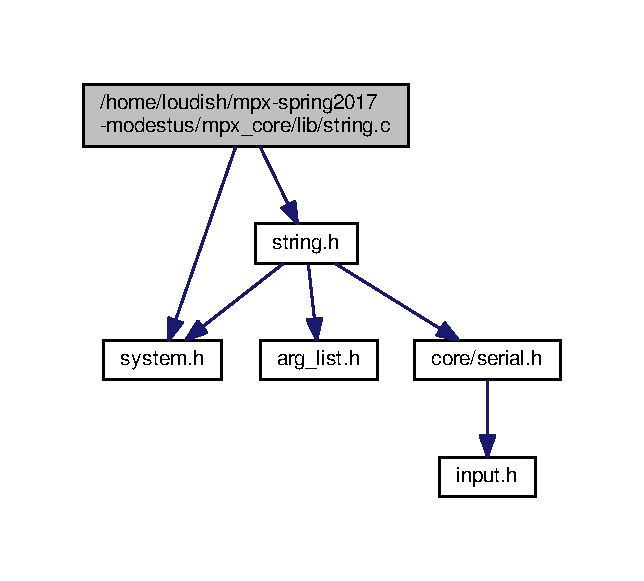
\includegraphics[width=309pt]{string_8c__incl}
\end{center}
\end{figure}
\subsection*{Functions}
\begin{DoxyCompactItemize}
\item 
int \hyperlink{string_8c_a2dee044e4e667b5b789b493abd21cfa4}{strlen} (const char $\ast$s)
\begin{DoxyCompactList}\small\item\em strlen returns the length of a string \end{DoxyCompactList}\item 
char $\ast$ \hyperlink{string_8c_a1eb9cae61e6a6282c28dbc298ef7297e}{strcpy} (char $\ast$s1, const char $\ast$s2)
\begin{DoxyCompactList}\small\item\em strcpy copies one string to another string \end{DoxyCompactList}\item 
int \hyperlink{string_8c_a30670a60464f77af17dfb353353d6df8}{atoi} (const char $\ast$s)
\begin{DoxyCompactList}\small\item\em atoi converts and A\+S\+C\+II string to an integer \end{DoxyCompactList}\item 
int \hyperlink{string_8c_a11bd144d7d44914099a3aeddf1c8567d}{strcmp} (const char $\ast$s1, const char $\ast$s2)
\begin{DoxyCompactList}\small\item\em strcmp compares two strings. \end{DoxyCompactList}\item 
char $\ast$ \hyperlink{string_8c_a8908188ae9fc2f05d993257ef001d553}{strcat} (char $\ast$s1, const char $\ast$s2)
\begin{DoxyCompactList}\small\item\em strcat concatenates the contents of one string onto another. \end{DoxyCompactList}\item 
int \hyperlink{string_8c_a0f3d37d605e9e6d4fc1853ff9d4b91bf}{isspace} (const char $\ast$c)
\begin{DoxyCompactList}\small\item\em isspace Determines if a character is a whitespace. \end{DoxyCompactList}\item 
void $\ast$ \hyperlink{string_8c_ace6ee45c30e71865e6eb635200379db9}{memset} (void $\ast$s, int c, \hyperlink{system_8h_a7c94ea6f8948649f8d181ae55911eeaf}{size\+\_\+t} n)
\begin{DoxyCompactList}\small\item\em memset Set a region of memory. \end{DoxyCompactList}\item 
char $\ast$ \hyperlink{string_8c_af1a867dcea42fc1215d0eddf19283ef3}{strtok} (char $\ast$s1, const char $\ast$s2)
\begin{DoxyCompactList}\small\item\em strtok Split string into tokens. \end{DoxyCompactList}\item 
int \hyperlink{string_8c_a4adae2826c898e6fded351cfebc561b4}{\+\_\+\+\_\+attribute\+\_\+\+\_\+} ((format(\hyperlink{string_8h_a0f459d16901ef591acaafa4b67fd4be5}{printf}, 3, 4)))
\begin{DoxyCompactList}\small\item\em sprintf print with format to specified string buffer \end{DoxyCompactList}\item 
int \hyperlink{string_8c_a397a240a4a5dc802bd2ba2054d25ae15}{int\+ToS} (const int $\ast$const i, char $\ast$buf, int buf\+Length)
\begin{DoxyCompactList}\small\item\em int\+ToS converts a signed integer to string \end{DoxyCompactList}\item 
char \hyperlink{string_8c_aca5e96bcd4ba56fb4d7ac75160f2161c}{is\+\_\+conversion\+\_\+specifier} (char c)
\begin{DoxyCompactList}\small\item\em is\+\_\+conversion\+\_\+specifier checks to see if the character is one of the standard printf formats \end{DoxyCompactList}\item 
int \hyperlink{string_8c_a1153bdbe1c0758a66d46bdefa2eb755d}{isnum} (const char c)
\begin{DoxyCompactList}\small\item\em isnum inline helper function to check if a character is represents an ascii number \end{DoxyCompactList}\end{DoxyCompactItemize}


\subsection{Function Documentation}
\index{string.\+c@{string.\+c}!\+\_\+\+\_\+attribute\+\_\+\+\_\+@{\+\_\+\+\_\+attribute\+\_\+\+\_\+}}
\index{\+\_\+\+\_\+attribute\+\_\+\+\_\+@{\+\_\+\+\_\+attribute\+\_\+\+\_\+}!string.\+c@{string.\+c}}
\subsubsection[{\texorpdfstring{\+\_\+\+\_\+attribute\+\_\+\+\_\+((format(printf, 3, 4)))}{__attribute__((format(printf, 3, 4)))}}]{\setlength{\rightskip}{0pt plus 5cm}int \+\_\+\+\_\+attribute\+\_\+\+\_\+ (
\begin{DoxyParamCaption}
\item[{(format({\bf printf}, 3, 4))}]{}
\end{DoxyParamCaption}
)}\hypertarget{string_8c_a4adae2826c898e6fded351cfebc561b4}{}\label{string_8c_a4adae2826c898e6fded351cfebc561b4}


sprintf print with format to specified string buffer 


\begin{DoxyParams}{Parameters}
{\em str} & a char $\ast$, place where the built string will be placed \\
\hline
{\em buf\+Length} & the size of the buffer of the char $\ast$, string writing will not exceed this value \\
\hline
{\em format} & a format string confirming to the std library format \\
\hline
{\em ...} & any number of parameters that will be printed according to the format. if wrong type is specified, behavior is undefined \\
\hline
\end{DoxyParams}
\begin{DoxyReturn}{Returns}
the number of characters placed in the output buffer 
\end{DoxyReturn}


Definition at line 225 of file string.\+c.



References arg\+\_\+list, atoi(), init\+\_\+arg\+\_\+list, int\+To\+S(), is\+\_\+conversion\+\_\+specifier(), isnum(), strcpy(), and strlen().


\begin{DoxyCode}
226 \{ 
227 
228     \textcolor{keywordflow}{if}(!str || bufLength <= 0) \{
229      \textcolor{keywordflow}{return} 0;
230     \}
231 
232     \hyperlink{arg__list_8h_abb821de0a9df92f33d827f2008093ddc}{arg\_list} list;
233     \hyperlink{arg__list_8h_a65f99a627ef400f9d875acca35dbac69}{init\_arg\_list}(list, format);
234 
235     \textcolor{keywordtype}{int} newStrIndex = 0;
236     \textcolor{keywordtype}{int} index, formatLength = \hyperlink{string_8c_a2dee044e4e667b5b789b493abd21cfa4}{strlen}(format);
237     \textcolor{keywordflow}{for}(index = 0; format[index] != \textcolor{charliteral}{'\(\backslash\)0'} && index < formatLength; index++)
238     \{
239      
240      \textcolor{comment}{//flag is -1 until fulfilled, flag is 0 if not requested}
241         \textcolor{keywordflow}{if}(format[index] == \textcolor{charliteral}{'%'})
242         \{
243             \textcolor{keywordtype}{char} leftJustified=0, alwaysAppendSign=0, subSignWithSpace=0, altForm=0, padWithZeros=0;
244             \textcolor{keywordtype}{int} minFieldWidth=0, precision=0;
245             (void)padWithZeros;
246             \textcolor{keywordflow}{for}(; !\hyperlink{string_8c_aca5e96bcd4ba56fb4d7ac75160f2161c}{is\_conversion\_specifier}(format[index]); index++)
247             \{
248                 \textcolor{keywordflow}{if}(format[index]==\textcolor{charliteral}{'\(\backslash\)0'})
249                 \{
250                     \textcolor{keywordflow}{return} 0; \textcolor{comment}{//if we reach the end of the string, exit as the format is missing}
251                 \}
252                 \textcolor{keywordflow}{if}(!minFieldWidth && !precision)
253                 \{
254                     \textcolor{keywordflow}{switch}(format[index])
255                     \{           
256                         \textcolor{keywordflow}{case} \textcolor{charliteral}{'-'}: leftJustified=1; \textcolor{keywordflow}{break};
257                         \textcolor{keywordflow}{case} \textcolor{charliteral}{'+'}: \textcolor{keywordflow}{if}(!leftJustified) \{alwaysAppendSign=1;\} \textcolor{keywordflow}{break};
258                         \textcolor{keywordflow}{case} \textcolor{charliteral}{' '}: \textcolor{keywordflow}{if}(!leftJustified && !alwaysAppendSign)\{subSignWithSpace=1;\} \textcolor{keywordflow}{break};
259                         \textcolor{keywordflow}{case} \textcolor{charliteral}{'#'}: \textcolor{keywordflow}{if}(!leftJustified && !alwaysAppendSign && !subSignWithSpace) \{altForm=1;\}
       \textcolor{keywordflow}{break};
260                         \textcolor{keywordflow}{case} \textcolor{charliteral}{'0'}: \textcolor{keywordflow}{if}(!leftJustified && !alwaysAppendSign && !subSignWithSpace && !altForm)\{
      padWithZeros=1;\} \textcolor{keywordflow}{break};
261                     \}
262                 \}
263                 \textcolor{keywordflow}{if}(format[index] == \textcolor{charliteral}{'.'})\{ precision = -1;\}
264                 \textcolor{keywordflow}{if}(\hyperlink{string_8c_a1153bdbe1c0758a66d46bdefa2eb755d}{isnum}(format[index])) \textcolor{comment}{//implement the * modifier here}
265                 \{
266                     \textcolor{keywordflow}{if}(precision==-1)
267                     \{ 
268                         precision = \hyperlink{string_8c_a30670a60464f77af17dfb353353d6df8}{atoi}(&format[index]); 
269                     \}
270                     \textcolor{keywordflow}{else} \textcolor{keywordflow}{if}(!minFieldWidth) 
271                     \{ 
272                         minFieldWidth = \hyperlink{string_8c_a30670a60464f77af17dfb353353d6df8}{atoi}(&format[index]); 
273                     \}
274                 \}
275             \}\textcolor{comment}{//finished parsing one conversion   }
276             \textcolor{comment}{//need to implement all modifiers}
277             \textcolor{keywordflow}{if}(format[index]==\textcolor{charliteral}{'d'})
278             \{
279                 newStrIndex += \hyperlink{string_8c_a397a240a4a5dc802bd2ba2054d25ae15}{intToS}((\textcolor{keywordtype}{int}*)next\_arg\_in\_list(&list, &format[index], 0), &str[
      newStrIndex], bufLength-newStrIndex) - 1;
280             \}
281             \textcolor{keywordflow}{else} \textcolor{keywordflow}{if}(format[index]==\textcolor{charliteral}{'c'})
282             \{
283                 str[newStrIndex]= **((\textcolor{keywordtype}{char}**)next\_arg\_in\_list(&list, &format[index], 0));
284                 newStrIndex++;
285             \}
286             \textcolor{keywordflow}{else} \textcolor{keywordflow}{if}(format[index]==\textcolor{charliteral}{'s'})
287             \{
288                 \textcolor{keywordtype}{char} *strToCopy = *((\textcolor{keywordtype}{char}**)next\_arg\_in\_list(&list, &format[index], 0));
289                 \textcolor{keywordtype}{int} lengthOfCopy = \hyperlink{string_8c_a2dee044e4e667b5b789b493abd21cfa4}{strlen}(strToCopy);
290                 \hyperlink{string_8c_a1eb9cae61e6a6282c28dbc298ef7297e}{strcpy}(&str[newStrIndex], strToCopy);
291                 newStrIndex += lengthOfCopy-1;
292             \}
293         \}
294         \textcolor{keywordflow}{else}
295         \{
296             str[newStrIndex] = format[index];
297             newStrIndex++;
298         \}
299     \}
300     str[newStrIndex]=0;
301     \textcolor{keywordflow}{return} newStrIndex;
302 \}
\end{DoxyCode}
\index{string.\+c@{string.\+c}!atoi@{atoi}}
\index{atoi@{atoi}!string.\+c@{string.\+c}}
\subsubsection[{\texorpdfstring{atoi(const char $\ast$s)}{atoi(const char *s)}}]{\setlength{\rightskip}{0pt plus 5cm}int atoi (
\begin{DoxyParamCaption}
\item[{const char $\ast$}]{s}
\end{DoxyParamCaption}
)}\hypertarget{string_8c_a30670a60464f77af17dfb353353d6df8}{}\label{string_8c_a30670a60464f77af17dfb353353d6df8}


atoi converts and A\+S\+C\+II string to an integer 


\begin{DoxyParams}{Parameters}
{\em s} & const char $\ast$s, character pointer to a string. \\
\hline
\end{DoxyParams}
\begin{DoxyReturn}{Returns}
the integer value of s. 
\end{DoxyReturn}


Definition at line 45 of file string.\+c.



Referenced by \+\_\+\+\_\+attribute\+\_\+\+\_\+(), kmain(), set\+Date(), and set\+Time().


\begin{DoxyCode}
46 \{
47     \textcolor{keywordtype}{int} num = 0;
48     \textcolor{keywordflow}{if}(!s)
49     \{
50         \textcolor{keywordflow}{return} 0;
51     \}
52 
53     \textcolor{keywordtype}{int} isNeg = ( *s == \textcolor{charliteral}{'-'});
54     \textcolor{keywordflow}{while}((*s >= \textcolor{charliteral}{'0'}) && (*s <= \textcolor{charliteral}{'9'} ))
55     \{
56         num = (num*10) + (*s - \textcolor{charliteral}{'0'});
57         s++;
58     \}
59     \textcolor{keywordflow}{if}(isNeg)
60     \{
61         num = num *(-1);
62     \}
63 
64     \textcolor{keywordflow}{return} num; \textcolor{comment}{// return integer}
65 \}
\end{DoxyCode}
\index{string.\+c@{string.\+c}!int\+ToS@{int\+ToS}}
\index{int\+ToS@{int\+ToS}!string.\+c@{string.\+c}}
\subsubsection[{\texorpdfstring{int\+To\+S(const int $\ast$const i, char $\ast$buf, int buf\+Length)}{intToS(const int *const i, char *buf, int bufLength)}}]{\setlength{\rightskip}{0pt plus 5cm}int int\+ToS (
\begin{DoxyParamCaption}
\item[{const int $\ast$const}]{i, }
\item[{char $\ast$}]{buf, }
\item[{int}]{buf\+Length}
\end{DoxyParamCaption}
)}\hypertarget{string_8c_a397a240a4a5dc802bd2ba2054d25ae15}{}\label{string_8c_a397a240a4a5dc802bd2ba2054d25ae15}


int\+ToS converts a signed integer to string 


\begin{DoxyParams}{Parameters}
{\em i} & integer to convert \\
\hline
{\em buf} & buf to place the converted string \\
\hline
{\em buf\+Length} & length of the buffer, string writing will not exceed this value \\
\hline
\end{DoxyParams}
\begin{DoxyReturn}{Returns}
num of characters written to buffer 
\end{DoxyReturn}


Definition at line 313 of file string.\+c.



References strlen().



Referenced by \+\_\+\+\_\+attribute\+\_\+\+\_\+().


\begin{DoxyCode}
314 \{
315     \textcolor{keywordflow}{if}(!buf)
316     \{ 
317         \textcolor{keywordflow}{return} 0; 
318     \}
319     
320     \textcolor{keywordtype}{int} cpy=*i;
321     \textcolor{keywordtype}{int} length = 1;
322     \textcolor{keywordflow}{if}(*i < 0)
323     \{ 
324         cpy*=-1;
325         length++;
326     \}
327     
328     \textcolor{keywordflow}{do}\{
329         length++;
330     \}\textcolor{keywordflow}{while}((cpy/=10)); \textcolor{comment}{//find total length of string}
331     
332     \textcolor{keywordflow}{if}(bufLength<length+1) \textcolor{comment}{//if the bufLength is less than the length+null term, return 0}
333     \{
334         \textcolor{keywordflow}{return} 0;
335     \}
336             
337     cpy=(*i<0)?(*i) * -1: *i;      \textcolor{comment}{//reset val copy}
338     length--;
339     buf[length]=\textcolor{charliteral}{'\(\backslash\)0'}; \textcolor{comment}{//insert null terminator at end of string}
340     length--;
341     \textcolor{keywordflow}{for}(; length >= 0; length--) \textcolor{comment}{//convert int to char and copy into buffer backwards}
342     \{
343         buf[length] = cpy%10 + \textcolor{charliteral}{'0'}; 
344         cpy/=10;
345     \}
346     \textcolor{keywordflow}{if}(*i<0)
347     \{
348         buf[0]=\textcolor{charliteral}{'-'};
349     \}
350     
351     \textcolor{keywordflow}{return} \hyperlink{string_8c_a2dee044e4e667b5b789b493abd21cfa4}{strlen}(buf);
352 \}
\end{DoxyCode}
\index{string.\+c@{string.\+c}!is\+\_\+conversion\+\_\+specifier@{is\+\_\+conversion\+\_\+specifier}}
\index{is\+\_\+conversion\+\_\+specifier@{is\+\_\+conversion\+\_\+specifier}!string.\+c@{string.\+c}}
\subsubsection[{\texorpdfstring{is\+\_\+conversion\+\_\+specifier(char c)}{is_conversion_specifier(char c)}}]{\setlength{\rightskip}{0pt plus 5cm}char is\+\_\+conversion\+\_\+specifier (
\begin{DoxyParamCaption}
\item[{char}]{c}
\end{DoxyParamCaption}
)}\hypertarget{string_8c_aca5e96bcd4ba56fb4d7ac75160f2161c}{}\label{string_8c_aca5e96bcd4ba56fb4d7ac75160f2161c}


is\+\_\+conversion\+\_\+specifier checks to see if the character is one of the standard printf formats 


\begin{DoxyParams}{Parameters}
{\em c} & character to check \\
\hline
\end{DoxyParams}
\begin{DoxyReturn}{Returns}
returns the character if the character is a format specifier, else returns 0 
\end{DoxyReturn}


Definition at line 359 of file string.\+c.



Referenced by \+\_\+\+\_\+attribute\+\_\+\+\_\+().


\begin{DoxyCode}
360 \{
361     \textcolor{keywordflow}{switch}(c)
362     \{
363         \textcolor{keywordflow}{case} \textcolor{charliteral}{'c'}: 
364         \textcolor{keywordflow}{case} \textcolor{charliteral}{'s'}: 
365         \textcolor{keywordflow}{case} \textcolor{charliteral}{'d'}: \textcolor{keywordflow}{case} \textcolor{charliteral}{'i'}: 
366         \textcolor{keywordflow}{case} \textcolor{charliteral}{'u'}: \textcolor{keywordflow}{case} \textcolor{charliteral}{'o'}: \textcolor{keywordflow}{case} \textcolor{charliteral}{'x'}: \textcolor{keywordflow}{case} \textcolor{charliteral}{'X'}: 
367         \textcolor{keywordflow}{case} \textcolor{charliteral}{'f'}: \textcolor{keywordflow}{case} \textcolor{charliteral}{'F'}: \textcolor{keywordflow}{case} \textcolor{charliteral}{'e'}: \textcolor{keywordflow}{case} \textcolor{charliteral}{'E'}: \textcolor{keywordflow}{case} \textcolor{charliteral}{'a'}: \textcolor{keywordflow}{case}\textcolor{charliteral}{'A'}: \textcolor{keywordflow}{case} \textcolor{charliteral}{'g'}: \textcolor{keywordflow}{case} \textcolor{charliteral}{'G'}:
368         \textcolor{keywordflow}{case} \textcolor{charliteral}{'p'}: 
369             \textcolor{keywordflow}{return} c; 
370         
371         \textcolor{keywordflow}{default}: \textcolor{keywordflow}{return} 0;
372     \}
373     \textcolor{keywordflow}{return} 0;
374 \}
\end{DoxyCode}
\index{string.\+c@{string.\+c}!isnum@{isnum}}
\index{isnum@{isnum}!string.\+c@{string.\+c}}
\subsubsection[{\texorpdfstring{isnum(const char c)}{isnum(const char c)}}]{\setlength{\rightskip}{0pt plus 5cm}int isnum (
\begin{DoxyParamCaption}
\item[{const char}]{c}
\end{DoxyParamCaption}
)\hspace{0.3cm}{\ttfamily [inline]}}\hypertarget{string_8c_a1153bdbe1c0758a66d46bdefa2eb755d}{}\label{string_8c_a1153bdbe1c0758a66d46bdefa2eb755d}


isnum inline helper function to check if a character is represents an ascii number 


\begin{DoxyParams}{Parameters}
{\em c} & character to check \\
\hline
\end{DoxyParams}
\begin{DoxyReturn}{Returns}
returns 1 if the character is an ascii number, else returns 0 
\end{DoxyReturn}


Definition at line 381 of file string.\+c.



Referenced by \+\_\+\+\_\+attribute\+\_\+\+\_\+().


\begin{DoxyCode}
382 \{
383    \textcolor{keywordflow}{return} ((c >= \textcolor{charliteral}{'0'}) && (c <= \textcolor{charliteral}{'9'}));
384 \}
\end{DoxyCode}
\index{string.\+c@{string.\+c}!isspace@{isspace}}
\index{isspace@{isspace}!string.\+c@{string.\+c}}
\subsubsection[{\texorpdfstring{isspace(const char $\ast$c)}{isspace(const char *c)}}]{\setlength{\rightskip}{0pt plus 5cm}int isspace (
\begin{DoxyParamCaption}
\item[{const char $\ast$}]{c}
\end{DoxyParamCaption}
)}\hypertarget{string_8c_a0f3d37d605e9e6d4fc1853ff9d4b91bf}{}\label{string_8c_a0f3d37d605e9e6d4fc1853ff9d4b91bf}


isspace Determines if a character is a whitespace. 


\begin{DoxyParams}{Parameters}
{\em c} & character to check. \\
\hline
\end{DoxyParams}
\begin{DoxyReturn}{Returns}
1 if it is a whitespace, 0 if it is not a whitespace. 
\end{DoxyReturn}


Definition at line 110 of file string.\+c.


\begin{DoxyCode}
111 \{
112   \textcolor{keywordflow}{if} (*c == \textcolor{charliteral}{' '}  ||
113       *c == \textcolor{charliteral}{'\(\backslash\)n'} ||
114       *c == \textcolor{charliteral}{'\(\backslash\)r'} ||
115       *c == \textcolor{charliteral}{'\(\backslash\)f'} ||
116       *c == \textcolor{charliteral}{'\(\backslash\)t'} ||
117       *c == \textcolor{charliteral}{'\(\backslash\)v'})\{
118     \textcolor{keywordflow}{return} 1;
119   \}
120   \textcolor{keywordflow}{return} 0;
121 \}
\end{DoxyCode}
\index{string.\+c@{string.\+c}!memset@{memset}}
\index{memset@{memset}!string.\+c@{string.\+c}}
\subsubsection[{\texorpdfstring{memset(void $\ast$s, int c, size\+\_\+t n)}{memset(void *s, int c, size_t n)}}]{\setlength{\rightskip}{0pt plus 5cm}void$\ast$ memset (
\begin{DoxyParamCaption}
\item[{void $\ast$}]{s, }
\item[{int}]{c, }
\item[{{\bf size\+\_\+t}}]{n}
\end{DoxyParamCaption}
)}\hypertarget{string_8c_ace6ee45c30e71865e6eb635200379db9}{}\label{string_8c_ace6ee45c30e71865e6eb635200379db9}


memset Set a region of memory. 


\begin{DoxyParams}{Parameters}
{\em s} & destination. \\
\hline
{\em c} & byte to write. \\
\hline
{\em n} & count. \\
\hline
\end{DoxyParams}
\begin{DoxyReturn}{Returns}
void. 
\end{DoxyReturn}


Definition at line 135 of file string.\+c.



Referenced by init\+\_\+idt(), and init\+\_\+paging().


\begin{DoxyCode}
136 \{
137   \textcolor{keywordtype}{unsigned} \textcolor{keywordtype}{char} *p = (\textcolor{keywordtype}{unsigned} \textcolor{keywordtype}{char} *) s;
138   \textcolor{keywordflow}{while}(n--)\{
139     *p++ = (\textcolor{keywordtype}{unsigned} char) c;
140   \}
141   \textcolor{keywordflow}{return} s;
142 \}
\end{DoxyCode}
\index{string.\+c@{string.\+c}!strcat@{strcat}}
\index{strcat@{strcat}!string.\+c@{string.\+c}}
\subsubsection[{\texorpdfstring{strcat(char $\ast$s1, const char $\ast$s2)}{strcat(char *s1, const char *s2)}}]{\setlength{\rightskip}{0pt plus 5cm}char$\ast$ strcat (
\begin{DoxyParamCaption}
\item[{char $\ast$}]{s1, }
\item[{const char $\ast$}]{s2}
\end{DoxyParamCaption}
)}\hypertarget{string_8c_a8908188ae9fc2f05d993257ef001d553}{}\label{string_8c_a8908188ae9fc2f05d993257ef001d553}


strcat concatenates the contents of one string onto another. 


\begin{DoxyParams}{Parameters}
{\em s1} & destination string. \\
\hline
{\em s2} & source string. \\
\hline
\end{DoxyParams}
\begin{DoxyReturn}{Returns}
The combined string s1 and s2. 
\end{DoxyReturn}


Definition at line 97 of file string.\+c.



Referenced by klogv(), kmain(), and kpanic().


\begin{DoxyCode}
98 \{
99   \textcolor{keywordtype}{char} *rc = s1;
100   \textcolor{keywordflow}{if} (*s1) \textcolor{keywordflow}{while}(*++s1);
101   \textcolor{keywordflow}{while}( (*s1++ = *s2++) );
102   \textcolor{keywordflow}{return} rc;
103 \}
\end{DoxyCode}
\index{string.\+c@{string.\+c}!strcmp@{strcmp}}
\index{strcmp@{strcmp}!string.\+c@{string.\+c}}
\subsubsection[{\texorpdfstring{strcmp(const char $\ast$s1, const char $\ast$s2)}{strcmp(const char *s1, const char *s2)}}]{\setlength{\rightskip}{0pt plus 5cm}int strcmp (
\begin{DoxyParamCaption}
\item[{const char $\ast$}]{s1, }
\item[{const char $\ast$}]{s2}
\end{DoxyParamCaption}
)}\hypertarget{string_8c_a11bd144d7d44914099a3aeddf1c8567d}{}\label{string_8c_a11bd144d7d44914099a3aeddf1c8567d}


strcmp compares two strings. 


\begin{DoxyParams}{Parameters}
{\em s1} & string 1 to compare. \\
\hline
{\em s2} & string 2 to compare. \\
\hline
\end{DoxyParams}
\begin{DoxyReturn}{Returns}
if the two strings are equal. If they are equal it will return 0, otherwise will return a non-\/zero integer. 
\end{DoxyReturn}


Definition at line 73 of file string.\+c.



Referenced by date(), exec\+\_\+comm(), help\+Date(), help\+Func(), help\+Time(), is\+Empty(), pcb\+Func(), pcb\+Search\+Func(), searchcomp\+Function(), string\+To\+Class(), and time().


\begin{DoxyCode}
74 \{
75 
76   \textcolor{comment}{// Remarks:}
77   \textcolor{comment}{// 1) If we made it to the end of both strings (i. e. our pointer points to a}
78   \textcolor{comment}{//    '\(\backslash\)0' character), the function will return 0}
79   \textcolor{comment}{// 2) If we didn't make it to the end of both strings, the function will}
80   \textcolor{comment}{//    return the difference of the characters at the first index of}
81   \textcolor{comment}{//    indifference.}
82   \textcolor{keywordtype}{int} i = 0;
83   \textcolor{keywordflow}{for}(; (s1[i]) && (s2[i]) && (s1[i]==s2[i]); i++)
84   \{
85   \}
86   
87   \textcolor{keywordflow}{return} s1[i]-s2[i];
88 \}
\end{DoxyCode}
\index{string.\+c@{string.\+c}!strcpy@{strcpy}}
\index{strcpy@{strcpy}!string.\+c@{string.\+c}}
\subsubsection[{\texorpdfstring{strcpy(char $\ast$s1, const char $\ast$s2)}{strcpy(char *s1, const char *s2)}}]{\setlength{\rightskip}{0pt plus 5cm}char$\ast$ strcpy (
\begin{DoxyParamCaption}
\item[{char $\ast$}]{s1, }
\item[{const char $\ast$}]{s2}
\end{DoxyParamCaption}
)}\hypertarget{string_8c_a1eb9cae61e6a6282c28dbc298ef7297e}{}\label{string_8c_a1eb9cae61e6a6282c28dbc298ef7297e}


strcpy copies one string to another string 


\begin{DoxyParams}{Parameters}
{\em s1} & destination string. Character pointer to a string. \\
\hline
{\em s2} & source string. Character pointer to a string. \\
\hline
\end{DoxyParams}
\begin{DoxyReturn}{Returns}
return s1. 
\end{DoxyReturn}


Definition at line 26 of file string.\+c.



Referenced by \+\_\+\+\_\+attribute\+\_\+\+\_\+(), init\+\_\+commhand(), parse\+\_\+comm(), serial\+\_\+poll(), and setup\+P\+C\+B().


\begin{DoxyCode}
27 \{
28   \textcolor{keywordflow}{while}(*s2 != \textcolor{charliteral}{'\(\backslash\)0'}) \{
29       *s1 = *s2;
30       s1++;
31       s2++;
32    \}
33    \textcolor{keywordflow}{if}(*s2 == \textcolor{charliteral}{'\(\backslash\)0'}) \{
34       
35       *s1 = *s2;
36    \}
37   \textcolor{keywordflow}{return} s1; \textcolor{comment}{// return pointer to destination string}
38 \}
\end{DoxyCode}
\index{string.\+c@{string.\+c}!strlen@{strlen}}
\index{strlen@{strlen}!string.\+c@{string.\+c}}
\subsubsection[{\texorpdfstring{strlen(const char $\ast$s)}{strlen(const char *s)}}]{\setlength{\rightskip}{0pt plus 5cm}int strlen (
\begin{DoxyParamCaption}
\item[{const char $\ast$}]{s}
\end{DoxyParamCaption}
)}\hypertarget{string_8c_a2dee044e4e667b5b789b493abd21cfa4}{}\label{string_8c_a2dee044e4e667b5b789b493abd21cfa4}


strlen returns the length of a string 


\begin{DoxyParams}{Parameters}
{\em s} & character pointer to a string \\
\hline
\end{DoxyParams}
\begin{DoxyReturn}{Returns}
the length of the string 
\end{DoxyReturn}


Definition at line 10 of file string.\+c.



Referenced by \+\_\+\+\_\+attribute\+\_\+\+\_\+(), help\+Date(), help\+Time(), int\+To\+S(), set\+Date(), set\+Time(), and setup\+P\+C\+B().


\begin{DoxyCode}
11 \{
12    \textcolor{keywordtype}{int} length = 0;
13    \textcolor{keywordflow}{while}(s[length] != \textcolor{charliteral}{'\(\backslash\)0'}) \{
14     length++;
15    \}
16    length++;
17   \textcolor{keywordflow}{return} length; \textcolor{comment}{// return length of string}
18 \}
\end{DoxyCode}
\index{string.\+c@{string.\+c}!strtok@{strtok}}
\index{strtok@{strtok}!string.\+c@{string.\+c}}
\subsubsection[{\texorpdfstring{strtok(char $\ast$s1, const char $\ast$s2)}{strtok(char *s1, const char *s2)}}]{\setlength{\rightskip}{0pt plus 5cm}char$\ast$ strtok (
\begin{DoxyParamCaption}
\item[{char $\ast$}]{s1, }
\item[{const char $\ast$}]{s2}
\end{DoxyParamCaption}
)}\hypertarget{string_8c_af1a867dcea42fc1215d0eddf19283ef3}{}\label{string_8c_af1a867dcea42fc1215d0eddf19283ef3}


strtok Split string into tokens. 


\begin{DoxyParams}{Parameters}
{\em s1} & String to split \\
\hline
{\em s2} & Delimeter. \\
\hline
\end{DoxyParams}
\begin{DoxyReturn}{Returns}
String split into delimeters. 
\end{DoxyReturn}


Definition at line 150 of file string.\+c.



References N\+U\+LL.



Referenced by parse\+\_\+comm().


\begin{DoxyCode}
151 \{
152   \textcolor{keyword}{static} \textcolor{keywordtype}{char} *tok\_tmp = \hyperlink{system_8h_a070d2ce7b6bb7e5c05602aa8c308d0c4}{NULL};
153   \textcolor{keyword}{const} \textcolor{keywordtype}{char} *p = s2;
154 
155   \textcolor{comment}{//new string}
156   \textcolor{keywordflow}{if} (s1!=\hyperlink{system_8h_a070d2ce7b6bb7e5c05602aa8c308d0c4}{NULL})\{
157     tok\_tmp = s1;
158   \}
159   \textcolor{comment}{//old string cont'd}
160   \textcolor{keywordflow}{else} \{
161     \textcolor{keywordflow}{if} (tok\_tmp==\hyperlink{system_8h_a070d2ce7b6bb7e5c05602aa8c308d0c4}{NULL})\{
162       \textcolor{keywordflow}{return} \hyperlink{system_8h_a070d2ce7b6bb7e5c05602aa8c308d0c4}{NULL};
163     \}
164     s1 = tok\_tmp;
165   \}
166 
167   \textcolor{comment}{//skip leading s2 characters}
168   \textcolor{keywordflow}{while} ( *p && *s1 )\{
169     \textcolor{keywordflow}{if} (*s1==*p)\{
170       ++s1;
171       p = s2;
172       \textcolor{keywordflow}{continue};
173     \}
174     ++p;
175   \}
176 
177   \textcolor{comment}{//no more to parse}
178   \textcolor{keywordflow}{if} (!*s1)\{
179     \textcolor{keywordflow}{return} (tok\_tmp = \hyperlink{system_8h_a070d2ce7b6bb7e5c05602aa8c308d0c4}{NULL});
180   \}
181 
182   \textcolor{comment}{//skip non-s2 characters}
183   tok\_tmp = s1;
184   \textcolor{keywordflow}{while} (*tok\_tmp)\{
185     p = s2;
186     \textcolor{keywordflow}{while} (*p)\{
187       \textcolor{keywordflow}{if} (*tok\_tmp==*p++)\{
188     *tok\_tmp++ = \textcolor{charliteral}{'\(\backslash\)0'};
189     \textcolor{keywordflow}{return} s1;
190       \}
191     \}
192     ++tok\_tmp;
193   \}
194 
195   \textcolor{comment}{//end of string}
196   tok\_tmp = \hyperlink{system_8h_a070d2ce7b6bb7e5c05602aa8c308d0c4}{NULL};
197   \textcolor{keywordflow}{return} s1;
198 \}
\end{DoxyCode}

\hypertarget{anim_8c}{}\section{/home/loudish/mpx-\/spring2017-\/modestus/mpx\+\_\+core/modules/\+R1/anim.c File Reference}
\label{anim_8c}\index{/home/loudish/mpx-\/spring2017-\/modestus/mpx\+\_\+core/modules/\+R1/anim.\+c@{/home/loudish/mpx-\/spring2017-\/modestus/mpx\+\_\+core/modules/\+R1/anim.\+c}}
{\ttfamily \#include $<$core/serial.\+h$>$}\\*
Include dependency graph for anim.\+c\+:\nopagebreak
\begin{figure}[H]
\begin{center}
\leavevmode
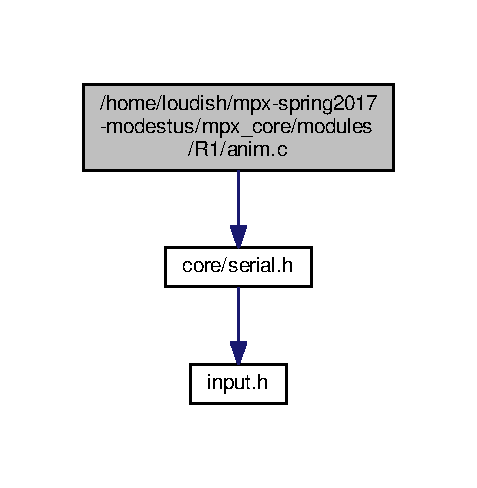
\includegraphics[width=229pt]{anim_8c__incl}
\end{center}
\end{figure}
\subsection*{Functions}
\begin{DoxyCompactItemize}
\item 
void \hyperlink{anim_8c_a251b758efbc88876a3f556ccc47fe40f}{busy\+\_\+wait} ()
\item 
void \hyperlink{anim_8c_a4953d1edcbbfc7e420c423ded1d5621a}{clear\+\_\+screen} ()
\item 
void \hyperlink{anim_8c_a07c0f5d662e90e4f24eda36ba3e46b16}{start\+\_\+up\+\_\+anim} ()
\end{DoxyCompactItemize}


\subsection{Function Documentation}
\index{anim.\+c@{anim.\+c}!busy\+\_\+wait@{busy\+\_\+wait}}
\index{busy\+\_\+wait@{busy\+\_\+wait}!anim.\+c@{anim.\+c}}
\subsubsection[{\texorpdfstring{busy\+\_\+wait()}{busy_wait()}}]{\setlength{\rightskip}{0pt plus 5cm}void busy\+\_\+wait (
\begin{DoxyParamCaption}
\item[{void}]{}
\end{DoxyParamCaption}
)}\hypertarget{anim_8c_a251b758efbc88876a3f556ccc47fe40f}{}\label{anim_8c_a251b758efbc88876a3f556ccc47fe40f}
R\+E-\/\+W\+R\+I\+TE T\+H\+IS SO T\+H\+AT IS IS M\+O\+RE E\+F\+F\+I\+C\+I\+E\+NT R\+U\+N\+N\+I\+NG 9999999 A\+SM C\+A\+L\+LS TO W\+A\+IT IS D\+U\+MB I\+N\+T\+E\+R\+R\+U\+P\+TS OR C\+H\+E\+CK T\+I\+ME W\+O\+U\+LD BE B\+E\+T\+T\+ER 

Definition at line 10 of file anim.\+c.



Referenced by start\+\_\+up\+\_\+anim().


\begin{DoxyCode}
10                  \{
11     \textcolor{keywordtype}{int} i = 0;
12     \textcolor{keywordflow}{for} (; i < 9999999; i++) \{
13         \textcolor{keyword}{asm} \textcolor{keyword}{volatile}(\textcolor{stringliteral}{"nop"});
14     \}
15 \}
\end{DoxyCode}
\index{anim.\+c@{anim.\+c}!clear\+\_\+screen@{clear\+\_\+screen}}
\index{clear\+\_\+screen@{clear\+\_\+screen}!anim.\+c@{anim.\+c}}
\subsubsection[{\texorpdfstring{clear\+\_\+screen()}{clear_screen()}}]{\setlength{\rightskip}{0pt plus 5cm}void clear\+\_\+screen (
\begin{DoxyParamCaption}
\item[{void}]{}
\end{DoxyParamCaption}
)}\hypertarget{anim_8c_a4953d1edcbbfc7e420c423ded1d5621a}{}\label{anim_8c_a4953d1edcbbfc7e420c423ded1d5621a}


Definition at line 17 of file anim.\+c.



References serial\+\_\+println().



Referenced by start\+\_\+up\+\_\+anim().


\begin{DoxyCode}
17                     \{
18     \hyperlink{serial_8h_a3514f7abff236a4e00a6c46021ce5e22}{serial\_println}(\textcolor{stringliteral}{"\(\backslash\)033[2J"});
19 \}
\end{DoxyCode}
\index{anim.\+c@{anim.\+c}!start\+\_\+up\+\_\+anim@{start\+\_\+up\+\_\+anim}}
\index{start\+\_\+up\+\_\+anim@{start\+\_\+up\+\_\+anim}!anim.\+c@{anim.\+c}}
\subsubsection[{\texorpdfstring{start\+\_\+up\+\_\+anim()}{start_up_anim()}}]{\setlength{\rightskip}{0pt plus 5cm}void start\+\_\+up\+\_\+anim (
\begin{DoxyParamCaption}
\item[{void}]{}
\end{DoxyParamCaption}
)}\hypertarget{anim_8c_a07c0f5d662e90e4f24eda36ba3e46b16}{}\label{anim_8c_a07c0f5d662e90e4f24eda36ba3e46b16}


Definition at line 21 of file anim.\+c.



References busy\+\_\+wait(), clear\+\_\+screen(), and serial\+\_\+println().



Referenced by kmain().


\begin{DoxyCode}
21                      \{
22     \hyperlink{serial_8h_a3514f7abff236a4e00a6c46021ce5e22}{serial\_println}(\textcolor{stringliteral}{"                 .------------.                                        "})
      ;
23     \hyperlink{serial_8h_a3514f7abff236a4e00a6c46021ce5e22}{serial\_println}(\textcolor{stringliteral}{"             .--'  o     . .   `--.                                "});
24     \hyperlink{serial_8h_a3514f7abff236a4e00a6c46021ce5e22}{serial\_println}(\textcolor{stringliteral}{"          .-'   .    O   .       . `-.                             "});
25     \hyperlink{serial_8h_a3514f7abff236a4e00a6c46021ce5e22}{serial\_println}(\textcolor{stringliteral}{"       .-'@   @@@@@@@   .  @@@@@      `-.                          "});
26     \hyperlink{serial_8h_a3514f7abff236a4e00a6c46021ce5e22}{serial\_println}(\textcolor{stringliteral}{"      /@@@  @@@@@@@@@@@   @@@@@@@   .    \(\backslash\)\(\backslash\)                        "});
27     \hyperlink{serial_8h_a3514f7abff236a4e00a6c46021ce5e22}{serial\_println}(\textcolor{stringliteral}{"    ./    o @@@@@@@@@@@   @@@@@@@       . \(\backslash\)\(\backslash\).                      "});
28     \hyperlink{serial_8h_a3514f7abff236a4e00a6c46021ce5e22}{serial\_println}(\textcolor{stringliteral}{"   /@@  o   @@@@@@@@@@@.   @@@@@@@   O      \(\backslash\)\(\backslash\)                     "});
29     \hyperlink{serial_8h_a3514f7abff236a4e00a6c46021ce5e22}{serial\_println}(\textcolor{stringliteral}{"  /@@@@   .   @@@@@@@o    @@@@@@@@@@     @@@ \(\backslash\)\(\backslash\)                    "});
30     \hyperlink{serial_8h_a3514f7abff236a4e00a6c46021ce5e22}{serial\_println}(\textcolor{stringliteral}{"  |@@@@@               . @@@@@@@@@@@@@ o @@@@|                     "});
31     \hyperlink{serial_8h_a3514f7abff236a4e00a6c46021ce5e22}{serial\_println}(\textcolor{stringliteral}{" /@@@@@  O  `.-./  .      @@@@@@@@@@@@    @@  \(\backslash\)\(\backslash\)                   "});
32     \hyperlink{serial_8h_a3514f7abff236a4e00a6c46021ce5e22}{serial\_println}(\textcolor{stringliteral}{" | @@@@    --`-'       o     @@@@@@@@ @@@@    |                   "});
33     \hyperlink{serial_8h_a3514f7abff236a4e00a6c46021ce5e22}{serial\_println}(\textcolor{stringliteral}{" |@ @@@        `    o      .  @@   . @@@@@@@  |                    "});
34     \hyperlink{serial_8h_a3514f7abff236a4e00a6c46021ce5e22}{serial\_println}(\textcolor{stringliteral}{" |       @@  @         .-.     @@@   @@@@@@@  |                   "});
35     \hyperlink{serial_8h_a3514f7abff236a4e00a6c46021ce5e22}{serial\_println}(\textcolor{stringliteral}{" \(\backslash\)\(\backslash\)  . @        @@@     `-'   . @@@@   @@@@  o /                   "});
36     \hyperlink{serial_8h_a3514f7abff236a4e00a6c46021ce5e22}{serial\_println}(\textcolor{stringliteral}{"  |      @@   @@@@@ .           @@   .       |                     "});
37     \hyperlink{serial_8h_a3514f7abff236a4e00a6c46021ce5e22}{serial\_println}(\textcolor{stringliteral}{"  \(\backslash\)\(\backslash\)     @@@@  @\(\backslash\)\(\backslash\)@@    /  .  O    .     o   . /                   "});
38     \hyperlink{serial_8h_a3514f7abff236a4e00a6c46021ce5e22}{serial\_println}(\textcolor{stringliteral}{"   \(\backslash\)\(\backslash\)  o  @@     \(\backslash\)\(\backslash\) \(\backslash\)\(\backslash\)  /         .    .       /                   "});
39     \hyperlink{serial_8h_a3514f7abff236a4e00a6c46021ce5e22}{serial\_println}(\textcolor{stringliteral}{"    `\(\backslash\)\(\backslash\)     .    .\(\backslash\)\(\backslash\).-.\_\_\_   .      .   .-. /'                     "});
40     \hyperlink{serial_8h_a3514f7abff236a4e00a6c46021ce5e22}{serial\_println}(\textcolor{stringliteral}{"      \(\backslash\)\(\backslash\)           `-'                `-' /                        "});
41     \hyperlink{serial_8h_a3514f7abff236a4e00a6c46021ce5e22}{serial\_println}(\textcolor{stringliteral}{"       `-.   o   / |     o    O   .   .-'                          "});
42     \hyperlink{serial_8h_a3514f7abff236a4e00a6c46021ce5e22}{serial\_println}(\textcolor{stringliteral}{"          `-.   /     .       .    .-'                             "});
43     \hyperlink{serial_8h_a3514f7abff236a4e00a6c46021ce5e22}{serial\_println}(\textcolor{stringliteral}{"             `--.       .      .--'                                "});
44     \hyperlink{serial_8h_a3514f7abff236a4e00a6c46021ce5e22}{serial\_println}(\textcolor{stringliteral}{"                 `------------'                                        "})
      ;
45     
46     \hyperlink{anim_8c_a251b758efbc88876a3f556ccc47fe40f}{busy\_wait}();
47     \hyperlink{anim_8c_a4953d1edcbbfc7e420c423ded1d5621a}{clear\_screen}();
48 
49     \hyperlink{serial_8h_a3514f7abff236a4e00a6c46021ce5e22}{serial\_println}(\textcolor{stringliteral}{"                  ------------.    "});
50     \hyperlink{serial_8h_a3514f7abff236a4e00a6c46021ce5e22}{serial\_println}(\textcolor{stringliteral}{"              --'  o     . .   `--.    "});
51     \hyperlink{serial_8h_a3514f7abff236a4e00a6c46021ce5e22}{serial\_println}(\textcolor{stringliteral}{"           -'   .    O   .       . `-.     "});
52     \hyperlink{serial_8h_a3514f7abff236a4e00a6c46021ce5e22}{serial\_println}(\textcolor{stringliteral}{"         '@   @@@@@@@   .  @@@@@      `-.  "});
53     \hyperlink{serial_8h_a3514f7abff236a4e00a6c46021ce5e22}{serial\_println}(\textcolor{stringliteral}{"        @@  @@@@@@@@@@@   @@@@@@@   .    \(\backslash\)\(\backslash\)    "});
54     \hyperlink{serial_8h_a3514f7abff236a4e00a6c46021ce5e22}{serial\_println}(\textcolor{stringliteral}{"          o @@@@@@@@@@@   @@@@@@@       . \(\backslash\)\(\backslash\).  "});
55     \hyperlink{serial_8h_a3514f7abff236a4e00a6c46021ce5e22}{serial\_println}(\textcolor{stringliteral}{"        o   @@@@@@@@@@@.   @@@@@@@   O      \(\backslash\)\(\backslash\)     "});
56     \hyperlink{serial_8h_a3514f7abff236a4e00a6c46021ce5e22}{serial\_println}(\textcolor{stringliteral}{"     @@   .   @@@@@@@o    @@@@@@@@@@     @@@ \(\backslash\)\(\backslash\)    "});
57     \hyperlink{serial_8h_a3514f7abff236a4e00a6c46021ce5e22}{serial\_println}(\textcolor{stringliteral}{"    @@@@               . @@@@@@@@@@@@@ o @@@@|     "});
58     \hyperlink{serial_8h_a3514f7abff236a4e00a6c46021ce5e22}{serial\_println}(\textcolor{stringliteral}{"    @@@  O  `.-./  .      @@@@@@@@@@@@    @@  \(\backslash\)\(\backslash\) "});
59     \hyperlink{serial_8h_a3514f7abff236a4e00a6c46021ce5e22}{serial\_println}(\textcolor{stringliteral}{"    @@@    --`-'       o     @@@@@@@@ @@@@    |    "});
60     \hyperlink{serial_8h_a3514f7abff236a4e00a6c46021ce5e22}{serial\_println}(\textcolor{stringliteral}{"    @@@        `    o      .  @@   . @@@@@@@  |    "});
61     \hyperlink{serial_8h_a3514f7abff236a4e00a6c46021ce5e22}{serial\_println}(\textcolor{stringliteral}{"         @@  @         .-.     @@@   @@@@@@@  |    "});
62     \hyperlink{serial_8h_a3514f7abff236a4e00a6c46021ce5e22}{serial\_println}(\textcolor{stringliteral}{"    . @        @@@     `-'   . @@@@   @@@@  o /    "});
63     \hyperlink{serial_8h_a3514f7abff236a4e00a6c46021ce5e22}{serial\_println}(\textcolor{stringliteral}{"         @@   @@@@@ .           @@   .       |     "});
64     \hyperlink{serial_8h_a3514f7abff236a4e00a6c46021ce5e22}{serial\_println}(\textcolor{stringliteral}{"        @@@@  @\(\backslash\)\(\backslash\)@@    /  .  O    .     o   . /    "});
65     \hyperlink{serial_8h_a3514f7abff236a4e00a6c46021ce5e22}{serial\_println}(\textcolor{stringliteral}{"      o  @@     \(\backslash\)\(\backslash\) \(\backslash\)\(\backslash\)  /         .    .       /    "});
66     \hyperlink{serial_8h_a3514f7abff236a4e00a6c46021ce5e22}{serial\_println}(\textcolor{stringliteral}{"           .    .\(\backslash\)\(\backslash\).-.\_\_\_   .      .   .-. /'  "});
67     \hyperlink{serial_8h_a3514f7abff236a4e00a6c46021ce5e22}{serial\_println}(\textcolor{stringliteral}{"                  `-'                `-' /     "});
68     \hyperlink{serial_8h_a3514f7abff236a4e00a6c46021ce5e22}{serial\_println}(\textcolor{stringliteral}{"         .   o   / |     o    O   .   .-'  "});
69     \hyperlink{serial_8h_a3514f7abff236a4e00a6c46021ce5e22}{serial\_println}(\textcolor{stringliteral}{"           -.   /     .       .    .-'     "});
70     \hyperlink{serial_8h_a3514f7abff236a4e00a6c46021ce5e22}{serial\_println}(\textcolor{stringliteral}{"              --.       .      .--'    "});
71     \hyperlink{serial_8h_a3514f7abff236a4e00a6c46021ce5e22}{serial\_println}(\textcolor{stringliteral}{"                  ------------'          "});
72 
73     \hyperlink{anim_8c_a251b758efbc88876a3f556ccc47fe40f}{busy\_wait}();
74     \hyperlink{anim_8c_a4953d1edcbbfc7e420c423ded1d5621a}{clear\_screen}();
75 
76     \hyperlink{serial_8h_a3514f7abff236a4e00a6c46021ce5e22}{serial\_println}(\textcolor{stringliteral}{"                    ----------.    "});
77     \hyperlink{serial_8h_a3514f7abff236a4e00a6c46021ce5e22}{serial\_println}(\textcolor{stringliteral}{"                   o     . .   `--.    "});
78     \hyperlink{serial_8h_a3514f7abff236a4e00a6c46021ce5e22}{serial\_println}(\textcolor{stringliteral}{"                .    O   .       . `-.     "});
79     \hyperlink{serial_8h_a3514f7abff236a4e00a6c46021ce5e22}{serial\_println}(\textcolor{stringliteral}{"              @@@@@@@   .  @@@@@      `-.  "});
80     \hyperlink{serial_8h_a3514f7abff236a4e00a6c46021ce5e22}{serial\_println}(\textcolor{stringliteral}{"             @@@@@@@@@@   @@@@@@@   .    \(\backslash\)\(\backslash\)    "});
81     \hyperlink{serial_8h_a3514f7abff236a4e00a6c46021ce5e22}{serial\_println}(\textcolor{stringliteral}{"            @@@@@@@@@@@   @@@@@@@       . \(\backslash\)\(\backslash\).  "});
82     \hyperlink{serial_8h_a3514f7abff236a4e00a6c46021ce5e22}{serial\_println}(\textcolor{stringliteral}{"            @@@@@@@@@@@.   @@@@@@@   O      \(\backslash\)\(\backslash\)     "});
83     \hyperlink{serial_8h_a3514f7abff236a4e00a6c46021ce5e22}{serial\_println}(\textcolor{stringliteral}{"              @@@@@@@o    @@@@@@@@@@     @@@ \(\backslash\)\(\backslash\)    "});
84     \hyperlink{serial_8h_a3514f7abff236a4e00a6c46021ce5e22}{serial\_println}(\textcolor{stringliteral}{"                       . @@@@@@@@@@@@@ o @@@@|     "});
85     \hyperlink{serial_8h_a3514f7abff236a4e00a6c46021ce5e22}{serial\_println}(\textcolor{stringliteral}{"            `.-./  .      @@@@@@@@@@@@    @@  \(\backslash\)\(\backslash\) "});
86     \hyperlink{serial_8h_a3514f7abff236a4e00a6c46021ce5e22}{serial\_println}(\textcolor{stringliteral}{"           --`-'       o     @@@@@@@@ @@@@    |    "});
87     \hyperlink{serial_8h_a3514f7abff236a4e00a6c46021ce5e22}{serial\_println}(\textcolor{stringliteral}{"               `    o      .  @@   . @@@@@@@  |    "});
88     \hyperlink{serial_8h_a3514f7abff236a4e00a6c46021ce5e22}{serial\_println}(\textcolor{stringliteral}{"          @  @         .-.     @@@   @@@@@@@  |    "});
89     \hyperlink{serial_8h_a3514f7abff236a4e00a6c46021ce5e22}{serial\_println}(\textcolor{stringliteral}{"               @@@     `-'   . @@@@   @@@@  o /    "});
90     \hyperlink{serial_8h_a3514f7abff236a4e00a6c46021ce5e22}{serial\_println}(\textcolor{stringliteral}{"              @@@@@ .           @@   .       |     "});
91     \hyperlink{serial_8h_a3514f7abff236a4e00a6c46021ce5e22}{serial\_println}(\textcolor{stringliteral}{"           @  @\(\backslash\)\(\backslash\)@@    /  .  O    .     o   . /    "});
92     \hyperlink{serial_8h_a3514f7abff236a4e00a6c46021ce5e22}{serial\_println}(\textcolor{stringliteral}{"                \(\backslash\)\(\backslash\) \(\backslash\)\(\backslash\)  /         .    .       /    "});
93     \hyperlink{serial_8h_a3514f7abff236a4e00a6c46021ce5e22}{serial\_println}(\textcolor{stringliteral}{"                .\(\backslash\)\(\backslash\).-.\_\_\_   .      .   .-. /'  "});
94     \hyperlink{serial_8h_a3514f7abff236a4e00a6c46021ce5e22}{serial\_println}(\textcolor{stringliteral}{"                  `-'                `-' /     "});
95     \hyperlink{serial_8h_a3514f7abff236a4e00a6c46021ce5e22}{serial\_println}(\textcolor{stringliteral}{"                 / |     o    O   .   .-'  "});
96     \hyperlink{serial_8h_a3514f7abff236a4e00a6c46021ce5e22}{serial\_println}(\textcolor{stringliteral}{"                /     .       .    .-'     "});
97     \hyperlink{serial_8h_a3514f7abff236a4e00a6c46021ce5e22}{serial\_println}(\textcolor{stringliteral}{"                        .      .--'    "});
98     \hyperlink{serial_8h_a3514f7abff236a4e00a6c46021ce5e22}{serial\_println}(\textcolor{stringliteral}{"                    ----------'          "});
99     
100     \hyperlink{anim_8c_a251b758efbc88876a3f556ccc47fe40f}{busy\_wait}();
101     \hyperlink{anim_8c_a4953d1edcbbfc7e420c423ded1d5621a}{clear\_screen}();
102 
103     \hyperlink{serial_8h_a3514f7abff236a4e00a6c46021ce5e22}{serial\_println}(\textcolor{stringliteral}{"                       -------.    "});
104     \hyperlink{serial_8h_a3514f7abff236a4e00a6c46021ce5e22}{serial\_println}(\textcolor{stringliteral}{"                         . .   `--.    "});
105     \hyperlink{serial_8h_a3514f7abff236a4e00a6c46021ce5e22}{serial\_println}(\textcolor{stringliteral}{"                         .       . `-.     "});
106     \hyperlink{serial_8h_a3514f7abff236a4e00a6c46021ce5e22}{serial\_println}(\textcolor{stringliteral}{"                        .  @@@@@      `-.  "});
107     \hyperlink{serial_8h_a3514f7abff236a4e00a6c46021ce5e22}{serial\_println}(\textcolor{stringliteral}{"                     @@   @@@@@@@   .    \(\backslash\)\(\backslash\)    "});
108     \hyperlink{serial_8h_a3514f7abff236a4e00a6c46021ce5e22}{serial\_println}(\textcolor{stringliteral}{"                     @@   @@@@@@@       . \(\backslash\)\(\backslash\).  "});
109     \hyperlink{serial_8h_a3514f7abff236a4e00a6c46021ce5e22}{serial\_println}(\textcolor{stringliteral}{"                    @@@.   @@@@@@@   O      \(\backslash\)\(\backslash\)     "});
110     \hyperlink{serial_8h_a3514f7abff236a4e00a6c46021ce5e22}{serial\_println}(\textcolor{stringliteral}{"                    @o    @@@@@@@@@@     @@@ \(\backslash\)\(\backslash\)    "});
111     \hyperlink{serial_8h_a3514f7abff236a4e00a6c46021ce5e22}{serial\_println}(\textcolor{stringliteral}{"                       . @@@@@@@@@@@@@ o @@@@|     "});
112     \hyperlink{serial_8h_a3514f7abff236a4e00a6c46021ce5e22}{serial\_println}(\textcolor{stringliteral}{"                          @@@@@@@@@@@@    @@  \(\backslash\)\(\backslash\)   "});
113     \hyperlink{serial_8h_a3514f7abff236a4e00a6c46021ce5e22}{serial\_println}(\textcolor{stringliteral}{"                       o     @@@@@@@@ @@@@    |    "});
114     \hyperlink{serial_8h_a3514f7abff236a4e00a6c46021ce5e22}{serial\_println}(\textcolor{stringliteral}{"                    o      .  @@   . @@@@@@@  |        "});
115     \hyperlink{serial_8h_a3514f7abff236a4e00a6c46021ce5e22}{serial\_println}(\textcolor{stringliteral}{"                       .-.     @@@   @@@@@@@  |    "});
116     \hyperlink{serial_8h_a3514f7abff236a4e00a6c46021ce5e22}{serial\_println}(\textcolor{stringliteral}{"                       `-'   . @@@@   @@@@  o /    "});
117     \hyperlink{serial_8h_a3514f7abff236a4e00a6c46021ce5e22}{serial\_println}(\textcolor{stringliteral}{"                    .           @@   .       |     "});
118     \hyperlink{serial_8h_a3514f7abff236a4e00a6c46021ce5e22}{serial\_println}(\textcolor{stringliteral}{"                      /  .  O    .     o   . /     "});
119     \hyperlink{serial_8h_a3514f7abff236a4e00a6c46021ce5e22}{serial\_println}(\textcolor{stringliteral}{"                     /         .    .       /  "});
120     \hyperlink{serial_8h_a3514f7abff236a4e00a6c46021ce5e22}{serial\_println}(\textcolor{stringliteral}{"                     \_\_\_   .      .   .-. /'   "});
121     \hyperlink{serial_8h_a3514f7abff236a4e00a6c46021ce5e22}{serial\_println}(\textcolor{stringliteral}{"                                     `-' /     "});
122     \hyperlink{serial_8h_a3514f7abff236a4e00a6c46021ce5e22}{serial\_println}(\textcolor{stringliteral}{"                         o    O   .   .-'  "});
123     \hyperlink{serial_8h_a3514f7abff236a4e00a6c46021ce5e22}{serial\_println}(\textcolor{stringliteral}{"                      .       .    .-'     "});
124     \hyperlink{serial_8h_a3514f7abff236a4e00a6c46021ce5e22}{serial\_println}(\textcolor{stringliteral}{"                        .      .--'    "});
125     \hyperlink{serial_8h_a3514f7abff236a4e00a6c46021ce5e22}{serial\_println}(\textcolor{stringliteral}{"                       -------'          "});
126 
127     \hyperlink{anim_8c_a251b758efbc88876a3f556ccc47fe40f}{busy\_wait}();
128     \hyperlink{anim_8c_a4953d1edcbbfc7e420c423ded1d5621a}{clear\_screen}();
129     
130     \hyperlink{serial_8h_a3514f7abff236a4e00a6c46021ce5e22}{serial\_println}(\textcolor{stringliteral}{"                         -----.    "});
131     \hyperlink{serial_8h_a3514f7abff236a4e00a6c46021ce5e22}{serial\_println}(\textcolor{stringliteral}{"                           .   `--.    "});
132     \hyperlink{serial_8h_a3514f7abff236a4e00a6c46021ce5e22}{serial\_println}(\textcolor{stringliteral}{"                                 . `-.     "});
133     \hyperlink{serial_8h_a3514f7abff236a4e00a6c46021ce5e22}{serial\_println}(\textcolor{stringliteral}{"                            @@@@      `-.  "});
134     \hyperlink{serial_8h_a3514f7abff236a4e00a6c46021ce5e22}{serial\_println}(\textcolor{stringliteral}{"                            @@@@@   .    \(\backslash\)\(\backslash\)    "});
135     \hyperlink{serial_8h_a3514f7abff236a4e00a6c46021ce5e22}{serial\_println}(\textcolor{stringliteral}{"                             @@@@       . \(\backslash\)\(\backslash\).  "});
136     \hyperlink{serial_8h_a3514f7abff236a4e00a6c46021ce5e22}{serial\_println}(\textcolor{stringliteral}{"                             @@@@@   O      \(\backslash\)\(\backslash\)     "});
137     \hyperlink{serial_8h_a3514f7abff236a4e00a6c46021ce5e22}{serial\_println}(\textcolor{stringliteral}{"                             @@@@@@@     @@@ \(\backslash\)\(\backslash\)    "});
138     \hyperlink{serial_8h_a3514f7abff236a4e00a6c46021ce5e22}{serial\_println}(\textcolor{stringliteral}{"                             @@@@@@@@@ o @@@@|     "});
139     \hyperlink{serial_8h_a3514f7abff236a4e00a6c46021ce5e22}{serial\_println}(\textcolor{stringliteral}{"                             @@@@@@@@@    @@  \(\backslash\)\(\backslash\) "});
140     \hyperlink{serial_8h_a3514f7abff236a4e00a6c46021ce5e22}{serial\_println}(\textcolor{stringliteral}{"                             @@@@@@@@ @@@@    |    "});
141     \hyperlink{serial_8h_a3514f7abff236a4e00a6c46021ce5e22}{serial\_println}(\textcolor{stringliteral}{"                              @@   . @@@@@@@  |    "});
142     \hyperlink{serial_8h_a3514f7abff236a4e00a6c46021ce5e22}{serial\_println}(\textcolor{stringliteral}{"                               @@@   @@@@@@@  |    "});
143     \hyperlink{serial_8h_a3514f7abff236a4e00a6c46021ce5e22}{serial\_println}(\textcolor{stringliteral}{"                             . @@@@   @@@@  o /    "});
144     \hyperlink{serial_8h_a3514f7abff236a4e00a6c46021ce5e22}{serial\_println}(\textcolor{stringliteral}{"                                @@   .       |     "});
145     \hyperlink{serial_8h_a3514f7abff236a4e00a6c46021ce5e22}{serial\_println}(\textcolor{stringliteral}{"                                 .     o   . /     "});
146     \hyperlink{serial_8h_a3514f7abff236a4e00a6c46021ce5e22}{serial\_println}(\textcolor{stringliteral}{"                               .    .       /  "});
147     \hyperlink{serial_8h_a3514f7abff236a4e00a6c46021ce5e22}{serial\_println}(\textcolor{stringliteral}{"                                  .   .-. /'   "});
148     \hyperlink{serial_8h_a3514f7abff236a4e00a6c46021ce5e22}{serial\_println}(\textcolor{stringliteral}{"                                     `-' /     "});
149     \hyperlink{serial_8h_a3514f7abff236a4e00a6c46021ce5e22}{serial\_println}(\textcolor{stringliteral}{"                              O   .   .-'  "});
150     \hyperlink{serial_8h_a3514f7abff236a4e00a6c46021ce5e22}{serial\_println}(\textcolor{stringliteral}{"                              .    .-'     "});
151     \hyperlink{serial_8h_a3514f7abff236a4e00a6c46021ce5e22}{serial\_println}(\textcolor{stringliteral}{"                               .--'    "});
152     \hyperlink{serial_8h_a3514f7abff236a4e00a6c46021ce5e22}{serial\_println}(\textcolor{stringliteral}{"                         -----'          "});
153 
154     \hyperlink{anim_8c_a251b758efbc88876a3f556ccc47fe40f}{busy\_wait}();
155     \hyperlink{anim_8c_a4953d1edcbbfc7e420c423ded1d5621a}{clear\_screen}();
156 
157     \hyperlink{serial_8h_a3514f7abff236a4e00a6c46021ce5e22}{serial\_println}(\textcolor{stringliteral}{"                           ---.    "});
158     \hyperlink{serial_8h_a3514f7abff236a4e00a6c46021ce5e22}{serial\_println}(\textcolor{stringliteral}{"                               `--.    "});
159     \hyperlink{serial_8h_a3514f7abff236a4e00a6c46021ce5e22}{serial\_println}(\textcolor{stringliteral}{"                                 . `-.     "});
160     \hyperlink{serial_8h_a3514f7abff236a4e00a6c46021ce5e22}{serial\_println}(\textcolor{stringliteral}{"                                      `-.  "});
161     \hyperlink{serial_8h_a3514f7abff236a4e00a6c46021ce5e22}{serial\_println}(\textcolor{stringliteral}{"                                    .    \(\backslash\)\(\backslash\)    "});
162     \hyperlink{serial_8h_a3514f7abff236a4e00a6c46021ce5e22}{serial\_println}(\textcolor{stringliteral}{"                                        . \(\backslash\)\(\backslash\).  "});
163     \hyperlink{serial_8h_a3514f7abff236a4e00a6c46021ce5e22}{serial\_println}(\textcolor{stringliteral}{"                                     O      \(\backslash\)\(\backslash\)     "});
164     \hyperlink{serial_8h_a3514f7abff236a4e00a6c46021ce5e22}{serial\_println}(\textcolor{stringliteral}{"                                         @@@ \(\backslash\)\(\backslash\)    "});
165     \hyperlink{serial_8h_a3514f7abff236a4e00a6c46021ce5e22}{serial\_println}(\textcolor{stringliteral}{"                                       o @@@@|        "});
166     \hyperlink{serial_8h_a3514f7abff236a4e00a6c46021ce5e22}{serial\_println}(\textcolor{stringliteral}{"                                          @@  \(\backslash\)\(\backslash\)   "});
167     \hyperlink{serial_8h_a3514f7abff236a4e00a6c46021ce5e22}{serial\_println}(\textcolor{stringliteral}{"                                      @@@@    |    "});
168     \hyperlink{serial_8h_a3514f7abff236a4e00a6c46021ce5e22}{serial\_println}(\textcolor{stringliteral}{"                                      @@@@@@  |    "});
169     \hyperlink{serial_8h_a3514f7abff236a4e00a6c46021ce5e22}{serial\_println}(\textcolor{stringliteral}{"                                      @@@@@@  |    "});
170     \hyperlink{serial_8h_a3514f7abff236a4e00a6c46021ce5e22}{serial\_println}(\textcolor{stringliteral}{"                                      @@@@  o /    "});
171     \hyperlink{serial_8h_a3514f7abff236a4e00a6c46021ce5e22}{serial\_println}(\textcolor{stringliteral}{"                                             |     "});
172     \hyperlink{serial_8h_a3514f7abff236a4e00a6c46021ce5e22}{serial\_println}(\textcolor{stringliteral}{"                                       o   . /     "});
173     \hyperlink{serial_8h_a3514f7abff236a4e00a6c46021ce5e22}{serial\_println}(\textcolor{stringliteral}{"                                            /  "});
174     \hyperlink{serial_8h_a3514f7abff236a4e00a6c46021ce5e22}{serial\_println}(\textcolor{stringliteral}{"                                      .-. /'   "});
175     \hyperlink{serial_8h_a3514f7abff236a4e00a6c46021ce5e22}{serial\_println}(\textcolor{stringliteral}{"                                     `-' /     "});
176     \hyperlink{serial_8h_a3514f7abff236a4e00a6c46021ce5e22}{serial\_println}(\textcolor{stringliteral}{"                                  .   .-'  "});
177     \hyperlink{serial_8h_a3514f7abff236a4e00a6c46021ce5e22}{serial\_println}(\textcolor{stringliteral}{"                                   .-'     "});
178     \hyperlink{serial_8h_a3514f7abff236a4e00a6c46021ce5e22}{serial\_println}(\textcolor{stringliteral}{"                               .--'    "});
179     \hyperlink{serial_8h_a3514f7abff236a4e00a6c46021ce5e22}{serial\_println}(\textcolor{stringliteral}{"                           ---'          "});
180 
181     \hyperlink{anim_8c_a251b758efbc88876a3f556ccc47fe40f}{busy\_wait}();
182     \hyperlink{anim_8c_a4953d1edcbbfc7e420c423ded1d5621a}{clear\_screen}();
183 
184     \hyperlink{serial_8h_a3514f7abff236a4e00a6c46021ce5e22}{serial\_println}(\textcolor{stringliteral}{"                             -.    "});
185     \hyperlink{serial_8h_a3514f7abff236a4e00a6c46021ce5e22}{serial\_println}(\textcolor{stringliteral}{"                                 -.    "});
186     \hyperlink{serial_8h_a3514f7abff236a4e00a6c46021ce5e22}{serial\_println}(\textcolor{stringliteral}{"                                    -.     "});
187     \hyperlink{serial_8h_a3514f7abff236a4e00a6c46021ce5e22}{serial\_println}(\textcolor{stringliteral}{"                                      `-.  "});
188     \hyperlink{serial_8h_a3514f7abff236a4e00a6c46021ce5e22}{serial\_println}(\textcolor{stringliteral}{"                                         \(\backslash\)\(\backslash\)    "});
189     \hyperlink{serial_8h_a3514f7abff236a4e00a6c46021ce5e22}{serial\_println}(\textcolor{stringliteral}{"                                          \(\backslash\)\(\backslash\).  "});
190     \hyperlink{serial_8h_a3514f7abff236a4e00a6c46021ce5e22}{serial\_println}(\textcolor{stringliteral}{"                                            \(\backslash\)\(\backslash\)     "});
191     \hyperlink{serial_8h_a3514f7abff236a4e00a6c46021ce5e22}{serial\_println}(\textcolor{stringliteral}{"                                           @ \(\backslash\)\(\backslash\)    "});
192     \hyperlink{serial_8h_a3514f7abff236a4e00a6c46021ce5e22}{serial\_println}(\textcolor{stringliteral}{"                                           @@|     "});
193     \hyperlink{serial_8h_a3514f7abff236a4e00a6c46021ce5e22}{serial\_println}(\textcolor{stringliteral}{"                                              \(\backslash\)\(\backslash\)        "});
194     \hyperlink{serial_8h_a3514f7abff236a4e00a6c46021ce5e22}{serial\_println}(\textcolor{stringliteral}{"                                              |    "});
195     \hyperlink{serial_8h_a3514f7abff236a4e00a6c46021ce5e22}{serial\_println}(\textcolor{stringliteral}{"                                              |    "});
196     \hyperlink{serial_8h_a3514f7abff236a4e00a6c46021ce5e22}{serial\_println}(\textcolor{stringliteral}{"                                              |    "});
197     \hyperlink{serial_8h_a3514f7abff236a4e00a6c46021ce5e22}{serial\_println}(\textcolor{stringliteral}{"                                            o /    "});
198     \hyperlink{serial_8h_a3514f7abff236a4e00a6c46021ce5e22}{serial\_println}(\textcolor{stringliteral}{"                                             |     "});
199     \hyperlink{serial_8h_a3514f7abff236a4e00a6c46021ce5e22}{serial\_println}(\textcolor{stringliteral}{"                                           . /     "});
200     \hyperlink{serial_8h_a3514f7abff236a4e00a6c46021ce5e22}{serial\_println}(\textcolor{stringliteral}{"                                            /  "});
201     \hyperlink{serial_8h_a3514f7abff236a4e00a6c46021ce5e22}{serial\_println}(\textcolor{stringliteral}{"                                          /'   "});
202     \hyperlink{serial_8h_a3514f7abff236a4e00a6c46021ce5e22}{serial\_println}(\textcolor{stringliteral}{"                                         /     "});
203     \hyperlink{serial_8h_a3514f7abff236a4e00a6c46021ce5e22}{serial\_println}(\textcolor{stringliteral}{"                                      .-'  "});
204     \hyperlink{serial_8h_a3514f7abff236a4e00a6c46021ce5e22}{serial\_println}(\textcolor{stringliteral}{"                                    -'     "});
205     \hyperlink{serial_8h_a3514f7abff236a4e00a6c46021ce5e22}{serial\_println}(\textcolor{stringliteral}{"                                 -'    "});
206     \hyperlink{serial_8h_a3514f7abff236a4e00a6c46021ce5e22}{serial\_println}(\textcolor{stringliteral}{"                             -'          "});
207 
208     \hyperlink{anim_8c_a251b758efbc88876a3f556ccc47fe40f}{busy\_wait}();
209     \hyperlink{anim_8c_a4953d1edcbbfc7e420c423ded1d5621a}{clear\_screen}();
210 
211     \hyperlink{serial_8h_a3514f7abff236a4e00a6c46021ce5e22}{serial\_println}(\textcolor{stringliteral}{"                  .    "});
212     \hyperlink{serial_8h_a3514f7abff236a4e00a6c46021ce5e22}{serial\_println}(\textcolor{stringliteral}{"             .     "});
213     \hyperlink{serial_8h_a3514f7abff236a4e00a6c46021ce5e22}{serial\_println}(\textcolor{stringliteral}{"          .    "});
214     \hyperlink{serial_8h_a3514f7abff236a4e00a6c46021ce5e22}{serial\_println}(\textcolor{stringliteral}{"       .-  "});
215     \hyperlink{serial_8h_a3514f7abff236a4e00a6c46021ce5e22}{serial\_println}(\textcolor{stringliteral}{"      /    "});
216     \hyperlink{serial_8h_a3514f7abff236a4e00a6c46021ce5e22}{serial\_println}(\textcolor{stringliteral}{"    .  "});
217     \hyperlink{serial_8h_a3514f7abff236a4e00a6c46021ce5e22}{serial\_println}(\textcolor{stringliteral}{"   /   "});
218     \hyperlink{serial_8h_a3514f7abff236a4e00a6c46021ce5e22}{serial\_println}(\textcolor{stringliteral}{"  /    "});
219     \hyperlink{serial_8h_a3514f7abff236a4e00a6c46021ce5e22}{serial\_println}(\textcolor{stringliteral}{"  |    "});
220     \hyperlink{serial_8h_a3514f7abff236a4e00a6c46021ce5e22}{serial\_println}(\textcolor{stringliteral}{" /          "});
221     \hyperlink{serial_8h_a3514f7abff236a4e00a6c46021ce5e22}{serial\_println}(\textcolor{stringliteral}{" |     "});
222     \hyperlink{serial_8h_a3514f7abff236a4e00a6c46021ce5e22}{serial\_println}(\textcolor{stringliteral}{" |     "});
223     \hyperlink{serial_8h_a3514f7abff236a4e00a6c46021ce5e22}{serial\_println}(\textcolor{stringliteral}{" |     "});
224     \hyperlink{serial_8h_a3514f7abff236a4e00a6c46021ce5e22}{serial\_println}(\textcolor{stringliteral}{" \(\backslash\)\(\backslash\)    "});
225     \hyperlink{serial_8h_a3514f7abff236a4e00a6c46021ce5e22}{serial\_println}(\textcolor{stringliteral}{"  |    "});
226     \hyperlink{serial_8h_a3514f7abff236a4e00a6c46021ce5e22}{serial\_println}(\textcolor{stringliteral}{"  \(\backslash\)\(\backslash\)   "});
227     \hyperlink{serial_8h_a3514f7abff236a4e00a6c46021ce5e22}{serial\_println}(\textcolor{stringliteral}{"   \(\backslash\)\(\backslash\)  "});
228     \hyperlink{serial_8h_a3514f7abff236a4e00a6c46021ce5e22}{serial\_println}(\textcolor{stringliteral}{"    `  "});
229     \hyperlink{serial_8h_a3514f7abff236a4e00a6c46021ce5e22}{serial\_println}(\textcolor{stringliteral}{"      \(\backslash\)\(\backslash\)   "});
230     \hyperlink{serial_8h_a3514f7abff236a4e00a6c46021ce5e22}{serial\_println}(\textcolor{stringliteral}{"       `-  "});
231     \hyperlink{serial_8h_a3514f7abff236a4e00a6c46021ce5e22}{serial\_println}(\textcolor{stringliteral}{"          `    "});
232     \hyperlink{serial_8h_a3514f7abff236a4e00a6c46021ce5e22}{serial\_println}(\textcolor{stringliteral}{"             `     "});
233     \hyperlink{serial_8h_a3514f7abff236a4e00a6c46021ce5e22}{serial\_println}(\textcolor{stringliteral}{"                 ` "});
234 
235     \hyperlink{anim_8c_a251b758efbc88876a3f556ccc47fe40f}{busy\_wait}();
236     \hyperlink{anim_8c_a4953d1edcbbfc7e420c423ded1d5621a}{clear\_screen}();
237 
238     \hyperlink{serial_8h_a3514f7abff236a4e00a6c46021ce5e22}{serial\_println}(\textcolor{stringliteral}{"                 .-    "});
239     \hyperlink{serial_8h_a3514f7abff236a4e00a6c46021ce5e22}{serial\_println}(\textcolor{stringliteral}{"             .-    "});
240     \hyperlink{serial_8h_a3514f7abff236a4e00a6c46021ce5e22}{serial\_println}(\textcolor{stringliteral}{"          .-   "});
241     \hyperlink{serial_8h_a3514f7abff236a4e00a6c46021ce5e22}{serial\_println}(\textcolor{stringliteral}{"       .-'@    "});
242     \hyperlink{serial_8h_a3514f7abff236a4e00a6c46021ce5e22}{serial\_println}(\textcolor{stringliteral}{"      /@@  "});
243     \hyperlink{serial_8h_a3514f7abff236a4e00a6c46021ce5e22}{serial\_println}(\textcolor{stringliteral}{"    ./     "});
244     \hyperlink{serial_8h_a3514f7abff236a4e00a6c46021ce5e22}{serial\_println}(\textcolor{stringliteral}{"   /@@     "});
245     \hyperlink{serial_8h_a3514f7abff236a4e00a6c46021ce5e22}{serial\_println}(\textcolor{stringliteral}{"  /@@@     "});
246     \hyperlink{serial_8h_a3514f7abff236a4e00a6c46021ce5e22}{serial\_println}(\textcolor{stringliteral}{"  |@@@     "});
247     \hyperlink{serial_8h_a3514f7abff236a4e00a6c46021ce5e22}{serial\_println}(\textcolor{stringliteral}{" /@@@   "});
248     \hyperlink{serial_8h_a3514f7abff236a4e00a6c46021ce5e22}{serial\_println}(\textcolor{stringliteral}{" | @@  "});
249     \hyperlink{serial_8h_a3514f7abff236a4e00a6c46021ce5e22}{serial\_println}(\textcolor{stringliteral}{" |@ @       "});
250     \hyperlink{serial_8h_a3514f7abff236a4e00a6c46021ce5e22}{serial\_println}(\textcolor{stringliteral}{" |     "});
251     \hyperlink{serial_8h_a3514f7abff236a4e00a6c46021ce5e22}{serial\_println}(\textcolor{stringliteral}{" \(\backslash\)\(\backslash\)  .     "});
252     \hyperlink{serial_8h_a3514f7abff236a4e00a6c46021ce5e22}{serial\_println}(\textcolor{stringliteral}{"  |        "});
253     \hyperlink{serial_8h_a3514f7abff236a4e00a6c46021ce5e22}{serial\_println}(\textcolor{stringliteral}{"  \(\backslash\)\(\backslash\)       "});
254     \hyperlink{serial_8h_a3514f7abff236a4e00a6c46021ce5e22}{serial\_println}(\textcolor{stringliteral}{"   \(\backslash\)\(\backslash\)  o   "});
255     \hyperlink{serial_8h_a3514f7abff236a4e00a6c46021ce5e22}{serial\_println}(\textcolor{stringliteral}{"    `\(\backslash\)\(\backslash\)    "});
256     \hyperlink{serial_8h_a3514f7abff236a4e00a6c46021ce5e22}{serial\_println}(\textcolor{stringliteral}{"      \(\backslash\)\(\backslash\)       "});
257     \hyperlink{serial_8h_a3514f7abff236a4e00a6c46021ce5e22}{serial\_println}(\textcolor{stringliteral}{"       `-.     "});
258     \hyperlink{serial_8h_a3514f7abff236a4e00a6c46021ce5e22}{serial\_println}(\textcolor{stringliteral}{"          `-   "});
259     \hyperlink{serial_8h_a3514f7abff236a4e00a6c46021ce5e22}{serial\_println}(\textcolor{stringliteral}{"             `-    "});
260     \hyperlink{serial_8h_a3514f7abff236a4e00a6c46021ce5e22}{serial\_println}(\textcolor{stringliteral}{"                 `-   "});
261 
262     \hyperlink{anim_8c_a251b758efbc88876a3f556ccc47fe40f}{busy\_wait}();
263     \hyperlink{anim_8c_a4953d1edcbbfc7e420c423ded1d5621a}{clear\_screen}();
264 
265     \hyperlink{serial_8h_a3514f7abff236a4e00a6c46021ce5e22}{serial\_println}(\textcolor{stringliteral}{"                 .---  "});
266     \hyperlink{serial_8h_a3514f7abff236a4e00a6c46021ce5e22}{serial\_println}(\textcolor{stringliteral}{"             .--'      "});
267     \hyperlink{serial_8h_a3514f7abff236a4e00a6c46021ce5e22}{serial\_println}(\textcolor{stringliteral}{"          .-'      "});
268     \hyperlink{serial_8h_a3514f7abff236a4e00a6c46021ce5e22}{serial\_println}(\textcolor{stringliteral}{"       .-'@   @    "});
269     \hyperlink{serial_8h_a3514f7abff236a4e00a6c46021ce5e22}{serial\_println}(\textcolor{stringliteral}{"      /@@@  @@     "});
270     \hyperlink{serial_8h_a3514f7abff236a4e00a6c46021ce5e22}{serial\_println}(\textcolor{stringliteral}{"    ./    o @  "});
271     \hyperlink{serial_8h_a3514f7abff236a4e00a6c46021ce5e22}{serial\_println}(\textcolor{stringliteral}{"   /@@  o   @  "});
272     \hyperlink{serial_8h_a3514f7abff236a4e00a6c46021ce5e22}{serial\_println}(\textcolor{stringliteral}{"  /@@@@   .    "});
273     \hyperlink{serial_8h_a3514f7abff236a4e00a6c46021ce5e22}{serial\_println}(\textcolor{stringliteral}{"  |@@@@@       "});
274     \hyperlink{serial_8h_a3514f7abff236a4e00a6c46021ce5e22}{serial\_println}(\textcolor{stringliteral}{" /@@@@@  O      "});
275     \hyperlink{serial_8h_a3514f7abff236a4e00a6c46021ce5e22}{serial\_println}(\textcolor{stringliteral}{" | @@@@        "});
276     \hyperlink{serial_8h_a3514f7abff236a4e00a6c46021ce5e22}{serial\_println}(\textcolor{stringliteral}{" |@ @@@             "});
277     \hyperlink{serial_8h_a3514f7abff236a4e00a6c46021ce5e22}{serial\_println}(\textcolor{stringliteral}{" |       @@    "});
278     \hyperlink{serial_8h_a3514f7abff236a4e00a6c46021ce5e22}{serial\_println}(\textcolor{stringliteral}{" \(\backslash\)\(\backslash\)  . @       "});
279     \hyperlink{serial_8h_a3514f7abff236a4e00a6c46021ce5e22}{serial\_println}(\textcolor{stringliteral}{"  |      @@    "});
280     \hyperlink{serial_8h_a3514f7abff236a4e00a6c46021ce5e22}{serial\_println}(\textcolor{stringliteral}{"  \(\backslash\)\(\backslash\)     @@@@  "});
281     \hyperlink{serial_8h_a3514f7abff236a4e00a6c46021ce5e22}{serial\_println}(\textcolor{stringliteral}{"   \(\backslash\)\(\backslash\)  o  @@       "});
282     \hyperlink{serial_8h_a3514f7abff236a4e00a6c46021ce5e22}{serial\_println}(\textcolor{stringliteral}{"    `\(\backslash\)\(\backslash\)     .      "});
283     \hyperlink{serial_8h_a3514f7abff236a4e00a6c46021ce5e22}{serial\_println}(\textcolor{stringliteral}{"      \(\backslash\)\(\backslash\)           "});
284     \hyperlink{serial_8h_a3514f7abff236a4e00a6c46021ce5e22}{serial\_println}(\textcolor{stringliteral}{"       `-.   o     "});
285     \hyperlink{serial_8h_a3514f7abff236a4e00a6c46021ce5e22}{serial\_println}(\textcolor{stringliteral}{"          `-.      "});
286     \hyperlink{serial_8h_a3514f7abff236a4e00a6c46021ce5e22}{serial\_println}(\textcolor{stringliteral}{"             `--.      "});
287     \hyperlink{serial_8h_a3514f7abff236a4e00a6c46021ce5e22}{serial\_println}(\textcolor{stringliteral}{"                 `---  "});
288 
289     \hyperlink{anim_8c_a251b758efbc88876a3f556ccc47fe40f}{busy\_wait}();
290     \hyperlink{anim_8c_a4953d1edcbbfc7e420c423ded1d5621a}{clear\_screen}();
291 
292     \hyperlink{serial_8h_a3514f7abff236a4e00a6c46021ce5e22}{serial\_println}(\textcolor{stringliteral}{"                 .-----    "});
293     \hyperlink{serial_8h_a3514f7abff236a4e00a6c46021ce5e22}{serial\_println}(\textcolor{stringliteral}{"             .--'  o       "});
294     \hyperlink{serial_8h_a3514f7abff236a4e00a6c46021ce5e22}{serial\_println}(\textcolor{stringliteral}{"          .-'   .    O     "});
295     \hyperlink{serial_8h_a3514f7abff236a4e00a6c46021ce5e22}{serial\_println}(\textcolor{stringliteral}{"       .-'@   @@@@@@@  "});
296     \hyperlink{serial_8h_a3514f7abff236a4e00a6c46021ce5e22}{serial\_println}(\textcolor{stringliteral}{"      /@@@  @@@@@@@@@  "});
297     \hyperlink{serial_8h_a3514f7abff236a4e00a6c46021ce5e22}{serial\_println}(\textcolor{stringliteral}{"    ./    o @@@@@@@@   "});
298     \hyperlink{serial_8h_a3514f7abff236a4e00a6c46021ce5e22}{serial\_println}(\textcolor{stringliteral}{"   /@@  o   @@@@@@@@   "});
299     \hyperlink{serial_8h_a3514f7abff236a4e00a6c46021ce5e22}{serial\_println}(\textcolor{stringliteral}{"  /@@@@   .   @@@@@@   "});
300     \hyperlink{serial_8h_a3514f7abff236a4e00a6c46021ce5e22}{serial\_println}(\textcolor{stringliteral}{"  |@@@@@               "});
301     \hyperlink{serial_8h_a3514f7abff236a4e00a6c46021ce5e22}{serial\_println}(\textcolor{stringliteral}{" /@@@@@  O  `.-./  .    "});
302     \hyperlink{serial_8h_a3514f7abff236a4e00a6c46021ce5e22}{serial\_println}(\textcolor{stringliteral}{" | @@@@    --`-'       "});
303     \hyperlink{serial_8h_a3514f7abff236a4e00a6c46021ce5e22}{serial\_println}(\textcolor{stringliteral}{" |@ @@@        `            "});
304     \hyperlink{serial_8h_a3514f7abff236a4e00a6c46021ce5e22}{serial\_println}(\textcolor{stringliteral}{" |       @@  @         "});
305     \hyperlink{serial_8h_a3514f7abff236a4e00a6c46021ce5e22}{serial\_println}(\textcolor{stringliteral}{" \(\backslash\)\(\backslash\)  . @        @@@    "});
306     \hyperlink{serial_8h_a3514f7abff236a4e00a6c46021ce5e22}{serial\_println}(\textcolor{stringliteral}{"  |      @@   @@@@@    "});
307     \hyperlink{serial_8h_a3514f7abff236a4e00a6c46021ce5e22}{serial\_println}(\textcolor{stringliteral}{"  \(\backslash\)\(\backslash\)     @@@@  @\(\backslash\)\(\backslash\)@@       "});
308     \hyperlink{serial_8h_a3514f7abff236a4e00a6c46021ce5e22}{serial\_println}(\textcolor{stringliteral}{"   \(\backslash\)\(\backslash\)  o  @@     \(\backslash\)\(\backslash\) \(\backslash\)\(\backslash\)     "});
309     \hyperlink{serial_8h_a3514f7abff236a4e00a6c46021ce5e22}{serial\_println}(\textcolor{stringliteral}{"    `\(\backslash\)\(\backslash\)     .    .\(\backslash\)\(\backslash\).-     "});
310     \hyperlink{serial_8h_a3514f7abff236a4e00a6c46021ce5e22}{serial\_println}(\textcolor{stringliteral}{"      \(\backslash\)\(\backslash\)           `-'     "});
311     \hyperlink{serial_8h_a3514f7abff236a4e00a6c46021ce5e22}{serial\_println}(\textcolor{stringliteral}{"       `-.   o   / |   "});
312     \hyperlink{serial_8h_a3514f7abff236a4e00a6c46021ce5e22}{serial\_println}(\textcolor{stringliteral}{"          `-.   /          "});
313     \hyperlink{serial_8h_a3514f7abff236a4e00a6c46021ce5e22}{serial\_println}(\textcolor{stringliteral}{"             `--.          "});
314     \hyperlink{serial_8h_a3514f7abff236a4e00a6c46021ce5e22}{serial\_println}(\textcolor{stringliteral}{"                 `-----  "});
315 
316     \hyperlink{anim_8c_a251b758efbc88876a3f556ccc47fe40f}{busy\_wait}();
317     \hyperlink{anim_8c_a4953d1edcbbfc7e420c423ded1d5621a}{clear\_screen}();
318 
319     \hyperlink{serial_8h_a3514f7abff236a4e00a6c46021ce5e22}{serial\_println}(\textcolor{stringliteral}{"                 .---------    "});
320     \hyperlink{serial_8h_a3514f7abff236a4e00a6c46021ce5e22}{serial\_println}(\textcolor{stringliteral}{"             .--'  o     . .       "});
321     \hyperlink{serial_8h_a3514f7abff236a4e00a6c46021ce5e22}{serial\_println}(\textcolor{stringliteral}{"          .-'   .    O   .         "});
322     \hyperlink{serial_8h_a3514f7abff236a4e00a6c46021ce5e22}{serial\_println}(\textcolor{stringliteral}{"       .-'@   @@@@@@@   .  @@@@@   "});
323     \hyperlink{serial_8h_a3514f7abff236a4e00a6c46021ce5e22}{serial\_println}(\textcolor{stringliteral}{"      /@@@  @@@@@@@@@@@   @@@@@@@  "});
324     \hyperlink{serial_8h_a3514f7abff236a4e00a6c46021ce5e22}{serial\_println}(\textcolor{stringliteral}{"    ./    o @@@@@@@@@@@   @@@@@@@      "});
325     \hyperlink{serial_8h_a3514f7abff236a4e00a6c46021ce5e22}{serial\_println}(\textcolor{stringliteral}{"   /@@  o   @@@@@@@@@@@.   @@@@@@@     "});
326     \hyperlink{serial_8h_a3514f7abff236a4e00a6c46021ce5e22}{serial\_println}(\textcolor{stringliteral}{"  /@@@@   .   @@@@@@@o    @@@@@@@@@    "});
327     \hyperlink{serial_8h_a3514f7abff236a4e00a6c46021ce5e22}{serial\_println}(\textcolor{stringliteral}{"  |@@@@@               . @@@@@@@@@@    "});
328     \hyperlink{serial_8h_a3514f7abff236a4e00a6c46021ce5e22}{serial\_println}(\textcolor{stringliteral}{" /@@@@@  O  `.-./  .      @@@@@@@@@        "});
329     \hyperlink{serial_8h_a3514f7abff236a4e00a6c46021ce5e22}{serial\_println}(\textcolor{stringliteral}{" | @@@@    --`-'       o     @@@@@@    "});
330     \hyperlink{serial_8h_a3514f7abff236a4e00a6c46021ce5e22}{serial\_println}(\textcolor{stringliteral}{" |@ @@@        `    o      .  @@        "});
331     \hyperlink{serial_8h_a3514f7abff236a4e00a6c46021ce5e22}{serial\_println}(\textcolor{stringliteral}{" |       @@  @         .-.     @@@     "});
332     \hyperlink{serial_8h_a3514f7abff236a4e00a6c46021ce5e22}{serial\_println}(\textcolor{stringliteral}{" \(\backslash\)\(\backslash\)  . @        @@@     `-'   . @@@@   "});
333     \hyperlink{serial_8h_a3514f7abff236a4e00a6c46021ce5e22}{serial\_println}(\textcolor{stringliteral}{"  |      @@   @@@@@ .           @@     "});
334     \hyperlink{serial_8h_a3514f7abff236a4e00a6c46021ce5e22}{serial\_println}(\textcolor{stringliteral}{"  \(\backslash\)\(\backslash\)     @@@@  @\(\backslash\)\(\backslash\)@@    /  .  O    .   "});
335     \hyperlink{serial_8h_a3514f7abff236a4e00a6c46021ce5e22}{serial\_println}(\textcolor{stringliteral}{"   \(\backslash\)\(\backslash\)  o  @@     \(\backslash\)\(\backslash\) \(\backslash\)\(\backslash\)  /         .    "});
336     \hyperlink{serial_8h_a3514f7abff236a4e00a6c46021ce5e22}{serial\_println}(\textcolor{stringliteral}{"    `\(\backslash\)\(\backslash\)     .    .\(\backslash\)\(\backslash\).-.\_\_\_   .         "});
337     \hyperlink{serial_8h_a3514f7abff236a4e00a6c46021ce5e22}{serial\_println}(\textcolor{stringliteral}{"      \(\backslash\)\(\backslash\)           `-'                 "});
338     \hyperlink{serial_8h_a3514f7abff236a4e00a6c46021ce5e22}{serial\_println}(\textcolor{stringliteral}{"       `-.   o   / |     o    O    "});
339     \hyperlink{serial_8h_a3514f7abff236a4e00a6c46021ce5e22}{serial\_println}(\textcolor{stringliteral}{"          `-.   /     .       .    "});
340     \hyperlink{serial_8h_a3514f7abff236a4e00a6c46021ce5e22}{serial\_println}(\textcolor{stringliteral}{"             `--.       .          "});
341     \hyperlink{serial_8h_a3514f7abff236a4e00a6c46021ce5e22}{serial\_println}(\textcolor{stringliteral}{"                 `---------   "});
342     
343     \hyperlink{anim_8c_a251b758efbc88876a3f556ccc47fe40f}{busy\_wait}();
344     \hyperlink{anim_8c_a4953d1edcbbfc7e420c423ded1d5621a}{clear\_screen}();
345 
346     \hyperlink{serial_8h_a3514f7abff236a4e00a6c46021ce5e22}{serial\_println}(\textcolor{stringliteral}{"                 .-----------  "});
347     \hyperlink{serial_8h_a3514f7abff236a4e00a6c46021ce5e22}{serial\_println}(\textcolor{stringliteral}{"             .--'  o     . .   `-  "});
348     \hyperlink{serial_8h_a3514f7abff236a4e00a6c46021ce5e22}{serial\_println}(\textcolor{stringliteral}{"          .-'   .    O   .       .     "});
349     \hyperlink{serial_8h_a3514f7abff236a4e00a6c46021ce5e22}{serial\_println}(\textcolor{stringliteral}{"       .-'@   @@@@@@@   .  @@@@@       "});
350     \hyperlink{serial_8h_a3514f7abff236a4e00a6c46021ce5e22}{serial\_println}(\textcolor{stringliteral}{"      /@@@  @@@@@@@@@@@   @@@@@@@   .      "});
351     \hyperlink{serial_8h_a3514f7abff236a4e00a6c46021ce5e22}{serial\_println}(\textcolor{stringliteral}{"    ./    o @@@@@@@@@@@   @@@@@@@          "});
352     \hyperlink{serial_8h_a3514f7abff236a4e00a6c46021ce5e22}{serial\_println}(\textcolor{stringliteral}{"   /@@  o   @@@@@@@@@@@.   @@@@@@@   O     "});
353     \hyperlink{serial_8h_a3514f7abff236a4e00a6c46021ce5e22}{serial\_println}(\textcolor{stringliteral}{"  /@@@@   .   @@@@@@@o    @@@@@@@@@@       "});
354     \hyperlink{serial_8h_a3514f7abff236a4e00a6c46021ce5e22}{serial\_println}(\textcolor{stringliteral}{"  |@@@@@               . @@@@@@@@@@@@@ o   "});
355     \hyperlink{serial_8h_a3514f7abff236a4e00a6c46021ce5e22}{serial\_println}(\textcolor{stringliteral}{" /@@@@@  O  `.-./  .      @@@@@@@@@@@@             "});
356     \hyperlink{serial_8h_a3514f7abff236a4e00a6c46021ce5e22}{serial\_println}(\textcolor{stringliteral}{" | @@@@    --`-'       o     @@@@@@@@ @@@@     "});
357     \hyperlink{serial_8h_a3514f7abff236a4e00a6c46021ce5e22}{serial\_println}(\textcolor{stringliteral}{" |@ @@@        `    o      .  @@   . @@@@@      "});
358     \hyperlink{serial_8h_a3514f7abff236a4e00a6c46021ce5e22}{serial\_println}(\textcolor{stringliteral}{" |       @@  @         .-.     @@@   @@@@@     "});
359     \hyperlink{serial_8h_a3514f7abff236a4e00a6c46021ce5e22}{serial\_println}(\textcolor{stringliteral}{" \(\backslash\)\(\backslash\)  . @        @@@     `-'   . @@@@   @@@@    "});
360     \hyperlink{serial_8h_a3514f7abff236a4e00a6c46021ce5e22}{serial\_println}(\textcolor{stringliteral}{"  |      @@   @@@@@ .           @@   .     "});
361     \hyperlink{serial_8h_a3514f7abff236a4e00a6c46021ce5e22}{serial\_println}(\textcolor{stringliteral}{"  \(\backslash\)\(\backslash\)     @@@@  @\(\backslash\)\(\backslash\)@@    /  .  O    .     o     "});
362     \hyperlink{serial_8h_a3514f7abff236a4e00a6c46021ce5e22}{serial\_println}(\textcolor{stringliteral}{"   \(\backslash\)\(\backslash\)  o  @@     \(\backslash\)\(\backslash\) \(\backslash\)\(\backslash\)  /         .    .       "});
363     \hyperlink{serial_8h_a3514f7abff236a4e00a6c46021ce5e22}{serial\_println}(\textcolor{stringliteral}{"    `\(\backslash\)\(\backslash\)     .    .\(\backslash\)\(\backslash\).-.\_\_\_   .      .   .  "});
364     \hyperlink{serial_8h_a3514f7abff236a4e00a6c46021ce5e22}{serial\_println}(\textcolor{stringliteral}{"      \(\backslash\)\(\backslash\)           `-'                `    "});
365     \hyperlink{serial_8h_a3514f7abff236a4e00a6c46021ce5e22}{serial\_println}(\textcolor{stringliteral}{"       `-.   o   / |     o    O   .    "});
366     \hyperlink{serial_8h_a3514f7abff236a4e00a6c46021ce5e22}{serial\_println}(\textcolor{stringliteral}{"          `-.   /     .       .        "});
367     \hyperlink{serial_8h_a3514f7abff236a4e00a6c46021ce5e22}{serial\_println}(\textcolor{stringliteral}{"             `--.       .      .-  "});
368     \hyperlink{serial_8h_a3514f7abff236a4e00a6c46021ce5e22}{serial\_println}(\textcolor{stringliteral}{"                 `-----------          "});
369 
370     \hyperlink{anim_8c_a251b758efbc88876a3f556ccc47fe40f}{busy\_wait}();
371     \hyperlink{anim_8c_a4953d1edcbbfc7e420c423ded1d5621a}{clear\_screen}();
372 
373     \hyperlink{serial_8h_a3514f7abff236a4e00a6c46021ce5e22}{serial\_println}(\textcolor{stringliteral}{"                 .------------     "});
374     \hyperlink{serial_8h_a3514f7abff236a4e00a6c46021ce5e22}{serial\_println}(\textcolor{stringliteral}{"             .--'  o     . .   `--.    "});
375     \hyperlink{serial_8h_a3514f7abff236a4e00a6c46021ce5e22}{serial\_println}(\textcolor{stringliteral}{"          .-'   .    O   .       . `-.     "});
376     \hyperlink{serial_8h_a3514f7abff236a4e00a6c46021ce5e22}{serial\_println}(\textcolor{stringliteral}{"       .-'@   @@@@@@@   .  @@@@@      `-   "});
377     \hyperlink{serial_8h_a3514f7abff236a4e00a6c46021ce5e22}{serial\_println}(\textcolor{stringliteral}{"      /@@@  @@@@@@@@@@@   @@@@@@@   .    \(\backslash\)\(\backslash\)    "});
378     \hyperlink{serial_8h_a3514f7abff236a4e00a6c46021ce5e22}{serial\_println}(\textcolor{stringliteral}{"    ./    o @@@@@@@@@@@   @@@@@@@       . \(\backslash\)\(\backslash\)   "});
379     \hyperlink{serial_8h_a3514f7abff236a4e00a6c46021ce5e22}{serial\_println}(\textcolor{stringliteral}{"   /@@  o   @@@@@@@@@@@.   @@@@@@@   O         "});
380     \hyperlink{serial_8h_a3514f7abff236a4e00a6c46021ce5e22}{serial\_println}(\textcolor{stringliteral}{"  /@@@@   .   @@@@@@@o    @@@@@@@@@@     @@@   "});
381     \hyperlink{serial_8h_a3514f7abff236a4e00a6c46021ce5e22}{serial\_println}(\textcolor{stringliteral}{"  |@@@@@               . @@@@@@@@@@@@@ o @@@@  "});
382     \hyperlink{serial_8h_a3514f7abff236a4e00a6c46021ce5e22}{serial\_println}(\textcolor{stringliteral}{" /@@@@@  O  `.-./  .      @@@@@@@@@@@@    @@       "});
383     \hyperlink{serial_8h_a3514f7abff236a4e00a6c46021ce5e22}{serial\_println}(\textcolor{stringliteral}{" | @@@@    --`-'       o     @@@@@@@@ @@@@         "});
384     \hyperlink{serial_8h_a3514f7abff236a4e00a6c46021ce5e22}{serial\_println}(\textcolor{stringliteral}{" |@ @@@        `    o      .  @@   . @@@@@@@       "});
385     \hyperlink{serial_8h_a3514f7abff236a4e00a6c46021ce5e22}{serial\_println}(\textcolor{stringliteral}{" |       @@  @         .-.     @@@   @@@@@@@       "});
386     \hyperlink{serial_8h_a3514f7abff236a4e00a6c46021ce5e22}{serial\_println}(\textcolor{stringliteral}{" \(\backslash\)\(\backslash\)  . @        @@@     `-'   . @@@@   @@@@  o     "});
387     \hyperlink{serial_8h_a3514f7abff236a4e00a6c46021ce5e22}{serial\_println}(\textcolor{stringliteral}{"  |      @@   @@@@@ .           @@   .         "});
388     \hyperlink{serial_8h_a3514f7abff236a4e00a6c46021ce5e22}{serial\_println}(\textcolor{stringliteral}{"  \(\backslash\)\(\backslash\)     @@@@  @\(\backslash\)\(\backslash\)@@    /  .  O    .     o   .     "});
389     \hyperlink{serial_8h_a3514f7abff236a4e00a6c46021ce5e22}{serial\_println}(\textcolor{stringliteral}{"   \(\backslash\)\(\backslash\)  o  @@     \(\backslash\)\(\backslash\) \(\backslash\)\(\backslash\)  /         .    .           "});
390     \hyperlink{serial_8h_a3514f7abff236a4e00a6c46021ce5e22}{serial\_println}(\textcolor{stringliteral}{"    `\(\backslash\)\(\backslash\)     .    .\(\backslash\)\(\backslash\).-.\_\_\_   .      .   .-. /  "});
391     \hyperlink{serial_8h_a3514f7abff236a4e00a6c46021ce5e22}{serial\_println}(\textcolor{stringliteral}{"      \(\backslash\)\(\backslash\)           `-'                `-' /    "});
392     \hyperlink{serial_8h_a3514f7abff236a4e00a6c46021ce5e22}{serial\_println}(\textcolor{stringliteral}{"       `-.   o   / |     o    O   .   .-   "});
393     \hyperlink{serial_8h_a3514f7abff236a4e00a6c46021ce5e22}{serial\_println}(\textcolor{stringliteral}{"          `-.   /     .       .    .-'     "});
394     \hyperlink{serial_8h_a3514f7abff236a4e00a6c46021ce5e22}{serial\_println}(\textcolor{stringliteral}{"             `--.       .      .--'    "});
395     \hyperlink{serial_8h_a3514f7abff236a4e00a6c46021ce5e22}{serial\_println}(\textcolor{stringliteral}{"                 `------------             "});
396 
397     \hyperlink{anim_8c_a251b758efbc88876a3f556ccc47fe40f}{busy\_wait}();
398     \hyperlink{anim_8c_a4953d1edcbbfc7e420c423ded1d5621a}{clear\_screen}();
399 
400     \hyperlink{serial_8h_a3514f7abff236a4e00a6c46021ce5e22}{serial\_println}(\textcolor{stringliteral}{"                 .------------.                                        "})
      ;
401     \hyperlink{serial_8h_a3514f7abff236a4e00a6c46021ce5e22}{serial\_println}(\textcolor{stringliteral}{"             .--'  o     . .   `--.                                "});
402     \hyperlink{serial_8h_a3514f7abff236a4e00a6c46021ce5e22}{serial\_println}(\textcolor{stringliteral}{"          .-'   .    O   .       . `-.                             "});
403     \hyperlink{serial_8h_a3514f7abff236a4e00a6c46021ce5e22}{serial\_println}(\textcolor{stringliteral}{"       .-'@   @@@@@@@   .  @@@@@      `-.                          "});
404     \hyperlink{serial_8h_a3514f7abff236a4e00a6c46021ce5e22}{serial\_println}(\textcolor{stringliteral}{"      /@@@  @@@@@@@@@@@   @@@@@@@   .    \(\backslash\)\(\backslash\)                        "});
405     \hyperlink{serial_8h_a3514f7abff236a4e00a6c46021ce5e22}{serial\_println}(\textcolor{stringliteral}{"    ./    o @@@@@@@@@@@   @@@@@@@       . \(\backslash\)\(\backslash\).                      "});
406     \hyperlink{serial_8h_a3514f7abff236a4e00a6c46021ce5e22}{serial\_println}(\textcolor{stringliteral}{"   /@@  o   @@@@@@@@@@@.   @@@@@@@   O      \(\backslash\)\(\backslash\)                     "});
407     \hyperlink{serial_8h_a3514f7abff236a4e00a6c46021ce5e22}{serial\_println}(\textcolor{stringliteral}{"  /@@@@   .   @@@@@@@o    @@@@@@@@@@     @@@ \(\backslash\)\(\backslash\)                    "});
408     \hyperlink{serial_8h_a3514f7abff236a4e00a6c46021ce5e22}{serial\_println}(\textcolor{stringliteral}{"  |@@@@@               . @@@@@@@@@@@@@ o @@@@|                     "});
409     \hyperlink{serial_8h_a3514f7abff236a4e00a6c46021ce5e22}{serial\_println}(\textcolor{stringliteral}{" /@@@@@  O  `.-./  .      @@@@@@@@@@@@    @@  \(\backslash\)\(\backslash\)                   "});
410     \hyperlink{serial_8h_a3514f7abff236a4e00a6c46021ce5e22}{serial\_println}(\textcolor{stringliteral}{" | @@@@    --`-'       o     @@@@@@@@ @@@@    |                   "});
411     \hyperlink{serial_8h_a3514f7abff236a4e00a6c46021ce5e22}{serial\_println}(\textcolor{stringliteral}{" |@ @@@        `    o      .  @@   . @@@@@@@  |   \(\backslash\)033[3m\(\backslash\)033[4mFull Moon
       OS\(\backslash\)033[0m"});
412     \hyperlink{serial_8h_a3514f7abff236a4e00a6c46021ce5e22}{serial\_println}(\textcolor{stringliteral}{" |       @@  @         .-.     @@@   @@@@@@@  |   Version: R1  "});
413     \hyperlink{serial_8h_a3514f7abff236a4e00a6c46021ce5e22}{serial\_println}(\textcolor{stringliteral}{" \(\backslash\)\(\backslash\)  . @        @@@     `-'   . @@@@   @@@@  o /                   "});
414     \hyperlink{serial_8h_a3514f7abff236a4e00a6c46021ce5e22}{serial\_println}(\textcolor{stringliteral}{"  |      @@   @@@@@ .           @@   .       |                     "});
415     \hyperlink{serial_8h_a3514f7abff236a4e00a6c46021ce5e22}{serial\_println}(\textcolor{stringliteral}{"  \(\backslash\)\(\backslash\)     @@@@  @\(\backslash\)\(\backslash\)@@    /  .  O    .     o   . /                   "});
416     \hyperlink{serial_8h_a3514f7abff236a4e00a6c46021ce5e22}{serial\_println}(\textcolor{stringliteral}{"   \(\backslash\)\(\backslash\)  o  @@     \(\backslash\)\(\backslash\) \(\backslash\)\(\backslash\)  /         .    .       /                   "});
417     \hyperlink{serial_8h_a3514f7abff236a4e00a6c46021ce5e22}{serial\_println}(\textcolor{stringliteral}{"    `\(\backslash\)\(\backslash\)     .    .\(\backslash\)\(\backslash\).-.\_\_\_   .      .   .-. /'                     "});
418     \hyperlink{serial_8h_a3514f7abff236a4e00a6c46021ce5e22}{serial\_println}(\textcolor{stringliteral}{"      \(\backslash\)\(\backslash\)           `-'                `-' /                        "});
419     \hyperlink{serial_8h_a3514f7abff236a4e00a6c46021ce5e22}{serial\_println}(\textcolor{stringliteral}{"       `-.   o   / |     o    O   .   .-'                          "});
420     \hyperlink{serial_8h_a3514f7abff236a4e00a6c46021ce5e22}{serial\_println}(\textcolor{stringliteral}{"          `-.   /     .       .    .-'                             "});
421     \hyperlink{serial_8h_a3514f7abff236a4e00a6c46021ce5e22}{serial\_println}(\textcolor{stringliteral}{"             `--.       .      .--'                                "});
422     \hyperlink{serial_8h_a3514f7abff236a4e00a6c46021ce5e22}{serial\_println}(\textcolor{stringliteral}{"                 `------------'                                        "})
      ;
423 \}
\end{DoxyCode}

\hypertarget{comm__list_8c}{}\section{/home/loudish/mpx-\/spring2017-\/modestus/mpx\+\_\+core/modules/\+R1/comm\+\_\+list.c File Reference}
\label{comm__list_8c}\index{/home/loudish/mpx-\/spring2017-\/modestus/mpx\+\_\+core/modules/\+R1/comm\+\_\+list.\+c@{/home/loudish/mpx-\/spring2017-\/modestus/mpx\+\_\+core/modules/\+R1/comm\+\_\+list.\+c}}
{\ttfamily \#include $<$comm\+\_\+vars.\+h$>$}\\*
{\ttfamily \#include $<$core/rtc.\+h$>$}\\*
{\ttfamily \#include $<$string.\+h$>$}\\*
{\ttfamily \#include $<$input.\+h$>$}\\*
{\ttfamily \#include \char`\"{}include/comm\+\_\+list.\+h\char`\"{}}\\*
{\ttfamily \#include $<$core/pcb.\+h$>$}\\*
{\ttfamily \#include $<$linked\+\_\+list.\+h$>$}\\*
Include dependency graph for comm\+\_\+list.\+c\+:\nopagebreak
\begin{figure}[H]
\begin{center}
\leavevmode
\includegraphics[width=350pt]{comm__list_8c__incl}
\end{center}
\end{figure}
\subsection*{Functions}
\begin{DoxyCompactItemize}
\item 
int \hyperlink{comm__list_8c_a63e5b5d633e0beec232fe5765124ad7e}{get\+Num\+Days\+In\+Month} (int month, int year)
\begin{DoxyCompactList}\small\item\em get\+Num\+Days\+In\+Month is a helper function to allow the easy retrieval of days in a month based on the month input by the user. \end{DoxyCompactList}\item 
int \hyperlink{comm__list_8c_a123c1c0d25a5a737a49a812d4bfd5d8d}{is\+Empty} (char parameters\mbox{[}$\,$\mbox{]}\mbox{[}\hyperlink{input_8h_a7a9a231e30b47bc0345749c8bd1e5077}{M\+A\+X\+\_\+\+L\+E\+N\+G\+TH}\mbox{]})
\item 
int \hyperlink{comm__list_8c_af4729cc64f3f6ec814af70e26c9ab9ca}{help\+Func} (char parameters\mbox{[}$\,$\mbox{]}\mbox{[}\hyperlink{input_8h_a7a9a231e30b47bc0345749c8bd1e5077}{M\+A\+X\+\_\+\+L\+E\+N\+G\+TH}\mbox{]})
\begin{DoxyCompactList}\small\item\em help\+Func compares the parameters after the \textquotesingle{}help\textquotesingle{} command and determines which function to call. \end{DoxyCompactList}\item 
void \hyperlink{comm__list_8c_a97ee70a8770dc30d06c744b24eb2fcfc}{help} ()
\begin{DoxyCompactList}\small\item\em help prints out a list of all possible commands and a brief description of what they do. \end{DoxyCompactList}\item 
int \hyperlink{comm__list_8c_aa0721512217377ef46085ce000a6daf4}{help\+Get\+Version} ()
\begin{DoxyCompactList}\small\item\em help\+Get\+Version prints the help instructions for version. Tells the user what the command and arguments for \textquotesingle{}version\textquotesingle{} are. \end{DoxyCompactList}\item 
void \hyperlink{comm__list_8c_a0f223b2f9d2c4887ab9d4943a565a20f}{help\+Get\+Date} ()
\begin{DoxyCompactList}\small\item\em help\+Get\+Date prints the help instructions for get date. Tells the user what the command and arguments for \textquotesingle{}get date\textquotesingle{} are. \end{DoxyCompactList}\item 
void \hyperlink{comm__list_8c_a315b74fd1af8e5c10ae8fea09a7f1343}{help\+Set\+Date} ()
\begin{DoxyCompactList}\small\item\em help\+Set\+Date prints the help instructions for set date. Tells the user what the command and arguments for \textquotesingle{}set date\textquotesingle{} are. \end{DoxyCompactList}\item 
void \hyperlink{comm__list_8c_ab023cd64db7b635c8e4048430fdd51c9}{help\+Get\+Time} ()
\begin{DoxyCompactList}\small\item\em help\+Get\+Time prints the help instructions for get time. Tells the user what the commands and arguments for \textquotesingle{}get time\textquotesingle{} are. \end{DoxyCompactList}\item 
void \hyperlink{comm__list_8c_a38bedc7695ebaf1fddec31cac15327b0}{help\+Set\+Time} ()
\begin{DoxyCompactList}\small\item\em help\+Set\+Time prints the help instructions for set time. Tells the user what the command and arguments for \textquotesingle{}set time\textquotesingle{} are. \end{DoxyCompactList}\item 
void \hyperlink{comm__list_8c_af128492f8bc92a7110f7e2de0bf26fa0}{help\+Shutdown} ()
\begin{DoxyCompactList}\small\item\em help\+Shutdown prints the help instructions for set date. Tells the user what the command and arguments for \textquotesingle{}set date\textquotesingle{} are. \end{DoxyCompactList}\item 
void \hyperlink{comm__list_8c_a6b64cff6b85c2b7edb02636de6e9d2ba}{help\+Version} ()
\begin{DoxyCompactList}\small\item\em help\+Version prints the help instructions for using the version command. No arguments are required. \end{DoxyCompactList}\item 
void \hyperlink{comm__list_8c_ae7390c4786bfe500bab96f1e0439902a}{help\+Date} (char parameters\mbox{[}$\,$\mbox{]}\mbox{[}\hyperlink{input_8h_a7a9a231e30b47bc0345749c8bd1e5077}{M\+A\+X\+\_\+\+L\+E\+N\+G\+TH}\mbox{]})
\item 
void \hyperlink{comm__list_8c_a4ade66f75a1cf0af90a2e983c6d4e656}{help\+Time} (char parameters\mbox{[}$\,$\mbox{]}\mbox{[}\hyperlink{input_8h_a7a9a231e30b47bc0345749c8bd1e5077}{M\+A\+X\+\_\+\+L\+E\+N\+G\+TH}\mbox{]})
\item 
void \hyperlink{comm__list_8c_a5c4cb1d2574709bc85d25706f5534cf4}{help\+Suspend\+P\+CB} ()
\begin{DoxyCompactList}\small\item\em help\+Suspend\+P\+CB prints the help instructions for the suspend\+P\+CB command. \end{DoxyCompactList}\item 
void \hyperlink{comm__list_8c_aba83fcaebd5841ba00582be3913d012d}{help\+Resume\+P\+CB} ()
\item 
void \hyperlink{comm__list_8c_ace39d9c4df8b991ae1db257969f511f3}{help\+Set\+Priority} ()
\item 
void \hyperlink{comm__list_8c_a8f9ff33592233864136430a150026353}{help\+Show\+P\+CB} ()
\item 
void \hyperlink{comm__list_8c_a20c49565baaff2aec112f4d99d63058f}{help\+Show\+All\+Processes} ()
\begin{DoxyCompactList}\small\item\em show\+All\+Processes shows all processes in the system. \end{DoxyCompactList}\item 
void \hyperlink{comm__list_8c_afc0abad04f83d121f3c7d8f4e08eade7}{help\+Show\+Ready\+Processes} ()
\begin{DoxyCompactList}\small\item\em show\+Ready\+Processes shows all processes that are ready, in the ready queue (linked list). \end{DoxyCompactList}\item 
void \hyperlink{comm__list_8c_a42841eb74573504baa22dd0c76ca83e9}{help\+Show\+Blocked\+Processes} ()
\begin{DoxyCompactList}\small\item\em show\+Blocked\+Processes shows all processes that are blocked. \end{DoxyCompactList}\item 
void \hyperlink{comm__list_8c_a72381b23fce4dc8d86d6ef7fbc440eda}{help\+Create\+P\+CB} ()
\begin{DoxyCompactList}\small\item\em create\+P\+CB creates a P\+CB \end{DoxyCompactList}\item 
void \hyperlink{comm__list_8c_a603af725d8289ae121f4ba45d55e654f}{help\+Delete\+P\+CB} ()
\begin{DoxyCompactList}\small\item\em delete\+P\+CB deletes the P\+CB requested by the user. \end{DoxyCompactList}\item 
void \hyperlink{comm__list_8c_a35106b0a99fb607930e3caa5f2a88974}{help\+Block\+P\+CB} ()
\begin{DoxyCompactList}\small\item\em block\+P\+CB blocks the specified P\+CB \end{DoxyCompactList}\item 
void \hyperlink{comm__list_8c_a2f4de74d76cc04ea63e4f253fcdf5aec}{help\+Unblock\+P\+CB} ()
\begin{DoxyCompactList}\small\item\em unblock\+P\+CB unblocks the specified P\+CB. \end{DoxyCompactList}\item 
int \hyperlink{comm__list_8c_ab21bb30658e69c3d4906e435384fa5fd}{version} (char parameters\mbox{[}$\,$\mbox{]}\mbox{[}\hyperlink{input_8h_a7a9a231e30b47bc0345749c8bd1e5077}{M\+A\+X\+\_\+\+L\+E\+N\+G\+TH}\mbox{]})
\begin{DoxyCompactList}\small\item\em version prints out the current version of the operating system. It will print out R1, R2, R3, ... depending on the current module. \end{DoxyCompactList}\item 
int \hyperlink{comm__list_8c_a2b5b0b260a749c7a0371b96f079b9d69}{date} (char parameters\mbox{[}$\,$\mbox{]}\mbox{[}\hyperlink{input_8h_a7a9a231e30b47bc0345749c8bd1e5077}{M\+A\+X\+\_\+\+L\+E\+N\+G\+TH}\mbox{]})
\item 
void \hyperlink{comm__list_8c_affb6f9c7b2c1d585677a5bba1da35c06}{get\+Date} ()
\begin{DoxyCompactList}\small\item\em get\+Date Get the current date from the system. \end{DoxyCompactList}\item 
void \hyperlink{comm__list_8c_abcb304e34ec42b6fa3df07249ce8c1b7}{set\+Date} (char parameters\mbox{[}$\,$\mbox{]}\mbox{[}\hyperlink{input_8h_a7a9a231e30b47bc0345749c8bd1e5077}{M\+A\+X\+\_\+\+L\+E\+N\+G\+TH}\mbox{]})
\begin{DoxyCompactList}\small\item\em set\+Date sets the system date using the input from the user. \end{DoxyCompactList}\item 
int \hyperlink{comm__list_8c_a5dac732108bdce081376535bd2d51221}{time} (char parameters\mbox{[}$\,$\mbox{]}\mbox{[}\hyperlink{input_8h_a7a9a231e30b47bc0345749c8bd1e5077}{M\+A\+X\+\_\+\+L\+E\+N\+G\+TH}\mbox{]})
\item 
void \hyperlink{comm__list_8c_a1c7c164fd3c7dea7004ece3c6251fc94}{get\+Time} ()
\begin{DoxyCompactList}\small\item\em get\+Time this function has the side-\/effect of printing the current time to the terminal. \end{DoxyCompactList}\item 
void \hyperlink{comm__list_8c_a684ac3c738428c05031f6b5c5b121d85}{set\+Time} (char parameters\mbox{[}$\,$\mbox{]}\mbox{[}\hyperlink{input_8h_a7a9a231e30b47bc0345749c8bd1e5077}{M\+A\+X\+\_\+\+L\+E\+N\+G\+TH}\mbox{]})
\begin{DoxyCompactList}\small\item\em set\+Time sets the current system time from the users input. \end{DoxyCompactList}\item 
int \hyperlink{comm__list_8c_a514416c2792fdc8614585266d618fbf8}{shutdown\+Func} (char parameters\mbox{[}$\,$\mbox{]}\mbox{[}\hyperlink{input_8h_a7a9a231e30b47bc0345749c8bd1e5077}{M\+A\+X\+\_\+\+L\+E\+N\+G\+TH}\mbox{]})
\item 
int \hyperlink{comm__list_8c_ac903af80a2e0afe97b30f5ca88a1505a}{pcb\+Func} (char parameters\mbox{[}$\,$\mbox{]}\mbox{[}\hyperlink{input_8h_a7a9a231e30b47bc0345749c8bd1e5077}{M\+A\+X\+\_\+\+L\+E\+N\+G\+TH}\mbox{]})
\item 
int \hyperlink{comm__list_8c_adb12aae9347bfdc11c97b2c89c448ce2}{suspend\+P\+CB} (char parameters\mbox{[}$\,$\mbox{]}\mbox{[}\hyperlink{input_8h_a7a9a231e30b47bc0345749c8bd1e5077}{M\+A\+X\+\_\+\+L\+E\+N\+G\+TH}\mbox{]})
\begin{DoxyCompactList}\small\item\em suspend\+P\+CB suspends the pcb passed in by the user \end{DoxyCompactList}\item 
int \hyperlink{comm__list_8c_a672eae99ab4e3da15306bc6df644bb50}{resume\+P\+CB} (char parameters\mbox{[}$\,$\mbox{]}\mbox{[}\hyperlink{input_8h_a7a9a231e30b47bc0345749c8bd1e5077}{M\+A\+X\+\_\+\+L\+E\+N\+G\+TH}\mbox{]})
\begin{DoxyCompactList}\small\item\em resume\+P\+CB resumes the P\+CB passed in by the user \end{DoxyCompactList}\item 
int \hyperlink{comm__list_8c_a3c30cca674e48a10a60180721d65cee0}{set\+Priority} (char parameters\mbox{[}$\,$\mbox{]}\mbox{[}\hyperlink{input_8h_a7a9a231e30b47bc0345749c8bd1e5077}{M\+A\+X\+\_\+\+L\+E\+N\+G\+TH}\mbox{]})
\begin{DoxyCompactList}\small\item\em set\+Priority sets the priority of a particular process \end{DoxyCompactList}\item 
int \hyperlink{comm__list_8c_a9b84e5992ebbf428fc68351c9453e52e}{show\+P\+CB} (char parameters\mbox{[}$\,$\mbox{]}\mbox{[}\hyperlink{input_8h_a7a9a231e30b47bc0345749c8bd1e5077}{M\+A\+X\+\_\+\+L\+E\+N\+G\+TH}\mbox{]})
\begin{DoxyCompactList}\small\item\em show\+P\+CB shows the process information for the process requested by the user \end{DoxyCompactList}\item 
int \hyperlink{comm__list_8c_a15a1fce149a24a3c2925b6ca44cb79c7}{show\+All\+Processes} (char parameters\mbox{[}$\,$\mbox{]}\mbox{[}\hyperlink{input_8h_a7a9a231e30b47bc0345749c8bd1e5077}{M\+A\+X\+\_\+\+L\+E\+N\+G\+TH}\mbox{]})
\begin{DoxyCompactList}\small\item\em show\+All\+Processes shows all processes in the system. \end{DoxyCompactList}\item 
int \hyperlink{comm__list_8c_abc0ff5bef60dfc962f4455492297a191}{show\+Ready\+Processes} (char parameters\mbox{[}$\,$\mbox{]}\mbox{[}\hyperlink{input_8h_a7a9a231e30b47bc0345749c8bd1e5077}{M\+A\+X\+\_\+\+L\+E\+N\+G\+TH}\mbox{]})
\begin{DoxyCompactList}\small\item\em show\+Ready\+Processes shows all processes that are ready, in the ready queue (linked list). \end{DoxyCompactList}\item 
int \hyperlink{comm__list_8c_aea06cb173ad17f9139253574d010d678}{show\+Blocked\+Processes} (char parameters\mbox{[}$\,$\mbox{]}\mbox{[}\hyperlink{input_8h_a7a9a231e30b47bc0345749c8bd1e5077}{M\+A\+X\+\_\+\+L\+E\+N\+G\+TH}\mbox{]})
\begin{DoxyCompactList}\small\item\em show\+Blocked\+Processes shows all processes that are blocked. \end{DoxyCompactList}\item 
int \hyperlink{comm__list_8c_ae147f79757d354c727a87836c71f1b05}{create\+P\+CB} (char parameters\mbox{[}$\,$\mbox{]}\mbox{[}\hyperlink{input_8h_a7a9a231e30b47bc0345749c8bd1e5077}{M\+A\+X\+\_\+\+L\+E\+N\+G\+TH}\mbox{]})
\begin{DoxyCompactList}\small\item\em create\+P\+CB creates a P\+CB \end{DoxyCompactList}\item 
int \hyperlink{comm__list_8c_a3602fa2889ad77ef2f323f6db3dd967e}{delete\+P\+CB} (char parameters\mbox{[}$\,$\mbox{]}\mbox{[}\hyperlink{input_8h_a7a9a231e30b47bc0345749c8bd1e5077}{M\+A\+X\+\_\+\+L\+E\+N\+G\+TH}\mbox{]})
\begin{DoxyCompactList}\small\item\em delete\+P\+CB deletes the P\+CB requested by the user. \end{DoxyCompactList}\item 
int \hyperlink{comm__list_8c_af8c8690ef4431e1629f9ab7c5539eeae}{block\+P\+CB} (char parameters\mbox{[}$\,$\mbox{]}\mbox{[}\hyperlink{input_8h_a7a9a231e30b47bc0345749c8bd1e5077}{M\+A\+X\+\_\+\+L\+E\+N\+G\+TH}\mbox{]})
\begin{DoxyCompactList}\small\item\em block\+P\+CB blocks the specified P\+CB \end{DoxyCompactList}\item 
int \hyperlink{comm__list_8c_ac26704b8c23bbe0e0fdf8e838915e29d}{unblock\+P\+CB} (char parameters\mbox{[}$\,$\mbox{]}\mbox{[}\hyperlink{input_8h_a7a9a231e30b47bc0345749c8bd1e5077}{M\+A\+X\+\_\+\+L\+E\+N\+G\+TH}\mbox{]})
\begin{DoxyCompactList}\small\item\em unblock\+P\+CB unblocks the specified P\+CB. \end{DoxyCompactList}\end{DoxyCompactItemize}


\subsection{Function Documentation}
\index{comm\+\_\+list.\+c@{comm\+\_\+list.\+c}!block\+P\+CB@{block\+P\+CB}}
\index{block\+P\+CB@{block\+P\+CB}!comm\+\_\+list.\+c@{comm\+\_\+list.\+c}}
\subsubsection[{\texorpdfstring{block\+P\+C\+B(char parameters[][M\+A\+X\+\_\+\+L\+E\+N\+G\+TH])}{blockPCB(char parameters[][MAX_LENGTH])}}]{\setlength{\rightskip}{0pt plus 5cm}int block\+P\+CB (
\begin{DoxyParamCaption}
\item[{char}]{parameters\mbox{[}$\,$\mbox{]}\mbox{[}\+M\+A\+X\+\_\+\+L\+E\+N\+G\+T\+H\mbox{]}}
\end{DoxyParamCaption}
)}\hypertarget{comm__list_8c_af8c8690ef4431e1629f9ab7c5539eeae}{}\label{comm__list_8c_af8c8690ef4431e1629f9ab7c5539eeae}


block\+P\+CB blocks the specified P\+CB 


\begin{DoxyParams}{Parameters}
{\em parameters} & \\
\hline
\end{DoxyParams}


Definition at line 738 of file comm\+\_\+list.\+c.



References B\+L\+O\+C\+K\+ED, and change\+Process\+State().



Referenced by pcb\+Func().


\begin{DoxyCode}
738                                             \{
739     \textcolor{keyword}{const} \textcolor{keywordtype}{char}* name = parameters[0];
740     \hyperlink{group___r2_ga83a5983d76f08725aadc23bf47930436}{changeProcessState}(name, \hyperlink{pcb_8h_a8461d6c03c00b03bad59b5a29d27b902a376c1b6a3f75d283a2efacf737438d61}{BLOCKED});
741     \textcolor{keywordflow}{return} 0;
742 \}
\end{DoxyCode}
\index{comm\+\_\+list.\+c@{comm\+\_\+list.\+c}!create\+P\+CB@{create\+P\+CB}}
\index{create\+P\+CB@{create\+P\+CB}!comm\+\_\+list.\+c@{comm\+\_\+list.\+c}}
\subsubsection[{\texorpdfstring{create\+P\+C\+B(char parameters[][M\+A\+X\+\_\+\+L\+E\+N\+G\+TH])}{createPCB(char parameters[][MAX_LENGTH])}}]{\setlength{\rightskip}{0pt plus 5cm}int create\+P\+CB (
\begin{DoxyParamCaption}
\item[{char}]{parameters\mbox{[}$\,$\mbox{]}\mbox{[}\+M\+A\+X\+\_\+\+L\+E\+N\+G\+T\+H\mbox{]}}
\end{DoxyParamCaption}
)}\hypertarget{comm__list_8c_ae147f79757d354c727a87836c71f1b05}{}\label{comm__list_8c_ae147f79757d354c727a87836c71f1b05}


create\+P\+CB creates a P\+CB 


\begin{DoxyParams}{Parameters}
{\em parameters} & \\
\hline
\end{DoxyParams}


Definition at line 714 of file comm\+\_\+list.\+c.



References setup\+P\+C\+B().



Referenced by pcb\+Func().


\begin{DoxyCode}
714                                              \{
715     \textcolor{keyword}{const} \textcolor{keywordtype}{char}* name = (\textcolor{keyword}{const} \textcolor{keywordtype}{char}*)parameters[0];
716     \hyperlink{pcb_8h_ab3268ce0bdfc94e5757917d42c73d9f1}{e\_PROCESS\_CLASS\_t} \textcolor{keyword}{class }= (\hyperlink{pcb_8h_ab3268ce0bdfc94e5757917d42c73d9f1}{e\_PROCESS\_CLASS\_t})parameters[1];
717     \hyperlink{pcb_8h_aade1badcda6beffd30258586dcad6550}{processPriority\_t} priority = (\hyperlink{pcb_8h_aade1badcda6beffd30258586dcad6550}{processPriority\_t})parameters[2];
718 
719     \hyperlink{pcb_8h_a9928a07bb6f59213464656fdab142e70}{setupPCB}(name, \textcolor{keyword}{class}, priority);
720     \textcolor{keywordflow}{return} 0;
721 \}
\end{DoxyCode}
\index{comm\+\_\+list.\+c@{comm\+\_\+list.\+c}!date@{date}}
\index{date@{date}!comm\+\_\+list.\+c@{comm\+\_\+list.\+c}}
\subsubsection[{\texorpdfstring{date(char parameters[][M\+A\+X\+\_\+\+L\+E\+N\+G\+TH])}{date(char parameters[][MAX_LENGTH])}}]{\setlength{\rightskip}{0pt plus 5cm}int date (
\begin{DoxyParamCaption}
\item[{char}]{parameters\mbox{[}$\,$\mbox{]}\mbox{[}\+M\+A\+X\+\_\+\+L\+E\+N\+G\+T\+H\mbox{]}}
\end{DoxyParamCaption}
)}\hypertarget{comm__list_8c_a2b5b0b260a749c7a0371b96f079b9d69}{}\label{comm__list_8c_a2b5b0b260a749c7a0371b96f079b9d69}


Definition at line 363 of file comm\+\_\+list.\+c.



References get\+Date(), serial\+\_\+println(), set\+Date(), and strcmp().



Referenced by init\+Cmd\+Array().


\begin{DoxyCode}
363                                         \{
364     \textcolor{keywordflow}{if}(!\hyperlink{string_8h_a11bd144d7d44914099a3aeddf1c8567d}{strcmp}(parameters[0],\textcolor{stringliteral}{"--get"})) \{
365         \hyperlink{comm__list_8c_affb6f9c7b2c1d585677a5bba1da35c06}{getDate}();
366     \} \textcolor{keywordflow}{else} \textcolor{keywordflow}{if}(!\hyperlink{string_8h_a11bd144d7d44914099a3aeddf1c8567d}{strcmp}(parameters[0],\textcolor{stringliteral}{"--set"})) \{
367         \hyperlink{comm__list_8c_abcb304e34ec42b6fa3df07249ce8c1b7}{setDate}(&parameters[1]);
368     \} \textcolor{keywordflow}{else} \{
369         \hyperlink{serial_8h_a3514f7abff236a4e00a6c46021ce5e22}{serial\_println}(\textcolor{stringliteral}{"ERROR HAS BEEN NOTICED"});
370     \}
371     \textcolor{keywordflow}{return} 0;
372 \}
\end{DoxyCode}
\index{comm\+\_\+list.\+c@{comm\+\_\+list.\+c}!delete\+P\+CB@{delete\+P\+CB}}
\index{delete\+P\+CB@{delete\+P\+CB}!comm\+\_\+list.\+c@{comm\+\_\+list.\+c}}
\subsubsection[{\texorpdfstring{delete\+P\+C\+B(char parameters[][M\+A\+X\+\_\+\+L\+E\+N\+G\+TH])}{deletePCB(char parameters[][MAX_LENGTH])}}]{\setlength{\rightskip}{0pt plus 5cm}int delete\+P\+CB (
\begin{DoxyParamCaption}
\item[{char}]{parameters\mbox{[}$\,$\mbox{]}\mbox{[}\+M\+A\+X\+\_\+\+L\+E\+N\+G\+T\+H\mbox{]}}
\end{DoxyParamCaption}
)}\hypertarget{comm__list_8c_a3602fa2889ad77ef2f323f6db3dd967e}{}\label{comm__list_8c_a3602fa2889ad77ef2f323f6db3dd967e}


delete\+P\+CB deletes the P\+CB requested by the user. 


\begin{DoxyParams}{Parameters}
{\em parameters} & \\
\hline
\end{DoxyParams}


Definition at line 727 of file comm\+\_\+list.\+c.



References find\+P\+C\+B(), and remove\+P\+C\+B().



Referenced by pcb\+Func().


\begin{DoxyCode}
727                                              \{
728     \textcolor{keyword}{const} \textcolor{keywordtype}{char}* name = (\textcolor{keyword}{const} \textcolor{keywordtype}{char}*)parameters[0];
729     \hyperlink{structpcb__t}{pcb\_t}* pcbToRem = \hyperlink{pcb_8h_a3ddbd6b7d5425cfb586dabc05862e9b1}{findPCB}(name);
730     \hyperlink{pcb_8h_aa7ccac95996427cc60aaee4eec35caf4}{removePCB}(pcbToRem);
731     \textcolor{keywordflow}{return} 0;
732 \}
\end{DoxyCode}
\index{comm\+\_\+list.\+c@{comm\+\_\+list.\+c}!get\+Date@{get\+Date}}
\index{get\+Date@{get\+Date}!comm\+\_\+list.\+c@{comm\+\_\+list.\+c}}
\subsubsection[{\texorpdfstring{get\+Date()}{getDate()}}]{\setlength{\rightskip}{0pt plus 5cm}void get\+Date (
\begin{DoxyParamCaption}
{}
\end{DoxyParamCaption}
)}\hypertarget{comm__list_8c_affb6f9c7b2c1d585677a5bba1da35c06}{}\label{comm__list_8c_affb6f9c7b2c1d585677a5bba1da35c06}


get\+Date Get the current date from the system. 

No parameters required, prints out a date. 

Definition at line 380 of file comm\+\_\+list.\+c.



References get\+\_\+date(), and printf.



Referenced by date(), and set\+Date().


\begin{DoxyCode}
380                \{
381     \textcolor{keywordtype}{int} month=0, day=0, year=0;
382     \hyperlink{rtc_8h_ab43f56447c49f42bb4baee3e59e2d1f9}{get\_date}(&day, &month, &year);
383     \hyperlink{string_8h_a0f459d16901ef591acaafa4b67fd4be5}{printf}(\textcolor{stringliteral}{"The current date is %d/%d/20%d UTC\(\backslash\)r\(\backslash\)n"}, day, month, year);
384 \}
\end{DoxyCode}
\index{comm\+\_\+list.\+c@{comm\+\_\+list.\+c}!get\+Num\+Days\+In\+Month@{get\+Num\+Days\+In\+Month}}
\index{get\+Num\+Days\+In\+Month@{get\+Num\+Days\+In\+Month}!comm\+\_\+list.\+c@{comm\+\_\+list.\+c}}
\subsubsection[{\texorpdfstring{get\+Num\+Days\+In\+Month(int month, int year)}{getNumDaysInMonth(int month, int year)}}]{\setlength{\rightskip}{0pt plus 5cm}int get\+Num\+Days\+In\+Month (
\begin{DoxyParamCaption}
\item[{int}]{month, }
\item[{int}]{year}
\end{DoxyParamCaption}
)}\hypertarget{comm__list_8c_a63e5b5d633e0beec232fe5765124ad7e}{}\label{comm__list_8c_a63e5b5d633e0beec232fe5765124ad7e}


get\+Num\+Days\+In\+Month is a helper function to allow the easy retrieval of days in a month based on the month input by the user. 


\begin{DoxyParams}{Parameters}
{\em month} & is an integer from 1-\/12 \\
\hline
{\em year} & is an integer representing the year to check if it\textquotesingle{}s a leap year \\
\hline
\end{DoxyParams}
\begin{DoxyReturn}{Returns}
the number of days in the corresponding month 
\end{DoxyReturn}


Definition at line 19 of file comm\+\_\+list.\+c.



Referenced by set\+Date().


\begin{DoxyCode}
19                                            \{
20     \textcolor{keywordtype}{int} days = 0;
21     \textcolor{keywordflow}{switch} (month) \{
22     \textcolor{keywordflow}{case} 01: \textcolor{keywordflow}{case} 3: \textcolor{keywordflow}{case} 5: \textcolor{keywordflow}{case} 7: \textcolor{keywordflow}{case} 8: \textcolor{keywordflow}{case} 10: \textcolor{keywordflow}{case} 12:
23         days = 31;
24         \textcolor{keywordflow}{break};
25     \textcolor{keywordflow}{case} 4: \textcolor{keywordflow}{case} 6: \textcolor{keywordflow}{case} 9: \textcolor{keywordflow}{case} 11:
26         days = 30;
27         \textcolor{keywordflow}{break};
28     \textcolor{keywordflow}{case} 2:
29         \textcolor{keywordflow}{if}(year%4==0)
30             days = 29;
31         \textcolor{keywordflow}{else}
32             days = 28;
33     \textcolor{keywordflow}{default}:
34         \textcolor{keywordflow}{break};
35     \}
36     \textcolor{keywordflow}{return} days;
37 \}
\end{DoxyCode}
\index{comm\+\_\+list.\+c@{comm\+\_\+list.\+c}!get\+Time@{get\+Time}}
\index{get\+Time@{get\+Time}!comm\+\_\+list.\+c@{comm\+\_\+list.\+c}}
\subsubsection[{\texorpdfstring{get\+Time()}{getTime()}}]{\setlength{\rightskip}{0pt plus 5cm}void get\+Time (
\begin{DoxyParamCaption}
{}
\end{DoxyParamCaption}
)}\hypertarget{comm__list_8c_a1c7c164fd3c7dea7004ece3c6251fc94}{}\label{comm__list_8c_a1c7c164fd3c7dea7004ece3c6251fc94}


get\+Time this function has the side-\/effect of printing the current time to the terminal. 

No parameters are required. 

Definition at line 444 of file comm\+\_\+list.\+c.



References get\+\_\+time(), serial\+\_\+print(), and sprintf().



Referenced by set\+Time(), and time().


\begin{DoxyCode}
444                \{
445     \textcolor{keywordtype}{int} hour=0, minutes=0, seconds=0;
446     \hyperlink{rtc_8h_a35fa24488cb7eb077e8dc995729202cf}{get\_time}(&hour, &minutes, &seconds);
447 
448     \textcolor{keywordtype}{char} buf[500]; \hyperlink{string_8h_ae9cac82f3293a00d8ec8705a3fc5cf64}{\(\backslash\)}
449 \hyperlink{string_8h_ae9cac82f3293a00d8ec8705a3fc5cf64}{    sprintf}(buf, 500, \textcolor{stringliteral}{"\(\backslash\)033[38;2;255;0;255mThe current time is %d:%d.%d UTC\(\backslash\)r\(\backslash\)n\(\backslash\)0
      33[38;2;255;255;255m"}, hour, minutes, seconds); \hyperlink{serial_8h_a995827efcd4dcfb780c9fbb9645410a4}{\(\backslash\)}
450 \hyperlink{serial_8h_a995827efcd4dcfb780c9fbb9645410a4}{    serial\_print}(buf);
451     \textcolor{comment}{//printf("\(\backslash\)033[38;2;255;0;255mThe current time is %d:%d.%d UTC\(\backslash\)r\(\backslash\)n\(\backslash\)033[38;2;255;255;255m", hour,
       minutes, seconds);}
452 \}
\end{DoxyCode}
\index{comm\+\_\+list.\+c@{comm\+\_\+list.\+c}!help@{help}}
\index{help@{help}!comm\+\_\+list.\+c@{comm\+\_\+list.\+c}}
\subsubsection[{\texorpdfstring{help()}{help()}}]{\setlength{\rightskip}{0pt plus 5cm}void help (
\begin{DoxyParamCaption}
{}
\end{DoxyParamCaption}
)}\hypertarget{comm__list_8c_a97ee70a8770dc30d06c744b24eb2fcfc}{}\label{comm__list_8c_a97ee70a8770dc30d06c744b24eb2fcfc}


help prints out a list of all possible commands and a brief description of what they do. 



Definition at line 80 of file comm\+\_\+list.\+c.



References serial\+\_\+println().



Referenced by help\+Func().


\begin{DoxyCode}
80             \{
81 
82     \hyperlink{serial_8h_a3514f7abff236a4e00a6c46021ce5e22}{serial\_println}(\textcolor{stringliteral}{"UNIX style commands\(\backslash\)r\(\backslash\)n"});
83     \hyperlink{serial_8h_a3514f7abff236a4e00a6c46021ce5e22}{serial\_println}(\textcolor{stringliteral}{"Command   | what it does"});
84     \hyperlink{serial_8h_a3514f7abff236a4e00a6c46021ce5e22}{serial\_println}(\textcolor{stringliteral}{"\_\_\_\_\_\_\_   | \_\_\_\_\_\_\_\_\_\_\_\_\_\_\_\_\_\_\_\_\_\_\_\_\_\_\_\_\_\_\_\_\_"});
85     \hyperlink{serial_8h_a3514f7abff236a4e00a6c46021ce5e22}{serial\_println}(\textcolor{stringliteral}{"version   | Get the current version of the OS"});
86     \hyperlink{serial_8h_a3514f7abff236a4e00a6c46021ce5e22}{serial\_println}(\textcolor{stringliteral}{"date      | Interact with the current system date"});
87     \hyperlink{serial_8h_a3514f7abff236a4e00a6c46021ce5e22}{serial\_println}(\textcolor{stringliteral}{"time      | Interact with the current system time"});
88     \hyperlink{serial_8h_a3514f7abff236a4e00a6c46021ce5e22}{serial\_println}(\textcolor{stringliteral}{"help      | Shows the command options"});
89     \hyperlink{serial_8h_a3514f7abff236a4e00a6c46021ce5e22}{serial\_println}(\textcolor{stringliteral}{"shutdown  | Shut down the system"});
90     \hyperlink{serial_8h_a3514f7abff236a4e00a6c46021ce5e22}{serial\_println}(\textcolor{stringliteral}{" "});
91     \hyperlink{serial_8h_a3514f7abff236a4e00a6c46021ce5e22}{serial\_println}(\textcolor{stringliteral}{"Type 'help [command]' to see what the command does and arguments it
       requires."});
92     \hyperlink{serial_8h_a3514f7abff236a4e00a6c46021ce5e22}{serial\_println}(\textcolor{stringliteral}{" "});
93 
94 \}
\end{DoxyCode}
\index{comm\+\_\+list.\+c@{comm\+\_\+list.\+c}!help\+Block\+P\+CB@{help\+Block\+P\+CB}}
\index{help\+Block\+P\+CB@{help\+Block\+P\+CB}!comm\+\_\+list.\+c@{comm\+\_\+list.\+c}}
\subsubsection[{\texorpdfstring{help\+Block\+P\+C\+B()}{helpBlockPCB()}}]{\setlength{\rightskip}{0pt plus 5cm}void help\+Block\+P\+CB (
\begin{DoxyParamCaption}
{}
\end{DoxyParamCaption}
)}\hypertarget{comm__list_8c_a35106b0a99fb607930e3caa5f2a88974}{}\label{comm__list_8c_a35106b0a99fb607930e3caa5f2a88974}


block\+P\+CB blocks the specified P\+CB 



Definition at line 329 of file comm\+\_\+list.\+c.


\begin{DoxyCode}
329                     \{
330 
331 \}
\end{DoxyCode}
\index{comm\+\_\+list.\+c@{comm\+\_\+list.\+c}!help\+Create\+P\+CB@{help\+Create\+P\+CB}}
\index{help\+Create\+P\+CB@{help\+Create\+P\+CB}!comm\+\_\+list.\+c@{comm\+\_\+list.\+c}}
\subsubsection[{\texorpdfstring{help\+Create\+P\+C\+B()}{helpCreatePCB()}}]{\setlength{\rightskip}{0pt plus 5cm}void help\+Create\+P\+CB (
\begin{DoxyParamCaption}
{}
\end{DoxyParamCaption}
)}\hypertarget{comm__list_8c_a72381b23fce4dc8d86d6ef7fbc440eda}{}\label{comm__list_8c_a72381b23fce4dc8d86d6ef7fbc440eda}


create\+P\+CB creates a P\+CB 


\begin{DoxyParams}{Parameters}
{\em parameters} & \\
\hline
\end{DoxyParams}


Definition at line 311 of file comm\+\_\+list.\+c.



References serial\+\_\+println().


\begin{DoxyCode}
311                      \{
312     \hyperlink{serial_8h_a3514f7abff236a4e00a6c46021ce5e22}{serial\_println}(\textcolor{stringliteral}{"Creates a PCB."});
313     \hyperlink{serial_8h_a3514f7abff236a4e00a6c46021ce5e22}{serial\_println}(\textcolor{stringliteral}{"Command: show -processes -b 'PCBname'"});
314     \hyperlink{serial_8h_a3514f7abff236a4e00a6c46021ce5e22}{serial\_println}(\textcolor{stringliteral}{"Arguments:"});
315     \hyperlink{serial_8h_a3514f7abff236a4e00a6c46021ce5e22}{serial\_println}(\textcolor{stringliteral}{"-processes -b -'the name of the PCB'"});
316     \hyperlink{serial_8h_a3514f7abff236a4e00a6c46021ce5e22}{serial\_println}(\textcolor{stringliteral}{" "});
317 \}
\end{DoxyCode}
\index{comm\+\_\+list.\+c@{comm\+\_\+list.\+c}!help\+Date@{help\+Date}}
\index{help\+Date@{help\+Date}!comm\+\_\+list.\+c@{comm\+\_\+list.\+c}}
\subsubsection[{\texorpdfstring{help\+Date(char parameters[][M\+A\+X\+\_\+\+L\+E\+N\+G\+TH])}{helpDate(char parameters[][MAX_LENGTH])}}]{\setlength{\rightskip}{0pt plus 5cm}void help\+Date (
\begin{DoxyParamCaption}
\item[{char}]{parameters\mbox{[}$\,$\mbox{]}\mbox{[}\+M\+A\+X\+\_\+\+L\+E\+N\+G\+T\+H\mbox{]}}
\end{DoxyParamCaption}
)}\hypertarget{comm__list_8c_ae7390c4786bfe500bab96f1e0439902a}{}\label{comm__list_8c_ae7390c4786bfe500bab96f1e0439902a}


Definition at line 194 of file comm\+\_\+list.\+c.



References serial\+\_\+println(), strcmp(), and strlen().



Referenced by help\+Func().


\begin{DoxyCode}
195 \{
196     \textcolor{keywordflow}{if}(\hyperlink{string_8h_a2dee044e4e667b5b789b493abd21cfa4}{strlen}(parameters[0]) <= 1)
197     \{
198         \hyperlink{serial_8h_a3514f7abff236a4e00a6c46021ce5e22}{serial\_println}(\textcolor{stringliteral}{"Retireves or Sets the system date"});
199         \hyperlink{serial_8h_a3514f7abff236a4e00a6c46021ce5e22}{serial\_println}(\textcolor{stringliteral}{"Command: 'date'"});
200         \hyperlink{serial_8h_a3514f7abff236a4e00a6c46021ce5e22}{serial\_println}(\textcolor{stringliteral}{"\(\backslash\)033[38;2;255;255;0mArguments available: \(\backslash\)033[38;2;255;0;0m--set,
       --get\(\backslash\)033[0m"});
201         \hyperlink{serial_8h_a3514f7abff236a4e00a6c46021ce5e22}{serial\_println}(\textcolor{stringliteral}{"Enter the command 'help date --get' or 'help date --set'"});
202     \}
203     \textcolor{keywordflow}{else} \textcolor{keywordflow}{if}(!\hyperlink{string_8h_a11bd144d7d44914099a3aeddf1c8567d}{strcmp}(parameters[0], \textcolor{stringliteral}{"set"}))
204     \{
205         \hyperlink{serial_8h_a3514f7abff236a4e00a6c46021ce5e22}{serial\_println}(\textcolor{stringliteral}{"Sets the system date"});
206         \hyperlink{serial_8h_a3514f7abff236a4e00a6c46021ce5e22}{serial\_println}(\textcolor{stringliteral}{"Command: 'date --set'"});
207         \hyperlink{serial_8h_a3514f7abff236a4e00a6c46021ce5e22}{serial\_println}(\textcolor{stringliteral}{"Usage: \(\backslash\)033[38;2;255;255;0m 'date --set' \(\backslash\)"DD/MM/YYYY\(\backslash\)" \(\backslash\)033[0m"});
208     \}
209     \textcolor{keywordflow}{else} \textcolor{keywordflow}{if}(!\hyperlink{string_8h_a11bd144d7d44914099a3aeddf1c8567d}{strcmp}(parameters[0], \textcolor{stringliteral}{"get"}))
210     \{
211         \hyperlink{serial_8h_a3514f7abff236a4e00a6c46021ce5e22}{serial\_println}(\textcolor{stringliteral}{"Gets the system date"});
212         \hyperlink{serial_8h_a3514f7abff236a4e00a6c46021ce5e22}{serial\_println}(\textcolor{stringliteral}{"Command: 'date --get'"});
213         \hyperlink{serial_8h_a3514f7abff236a4e00a6c46021ce5e22}{serial\_println}(\textcolor{stringliteral}{"Usage: \(\backslash\)033[38;2;255;255;0m 'date --get' \(\backslash\)033[0m"});
214     \}
215 \}
\end{DoxyCode}
\index{comm\+\_\+list.\+c@{comm\+\_\+list.\+c}!help\+Delete\+P\+CB@{help\+Delete\+P\+CB}}
\index{help\+Delete\+P\+CB@{help\+Delete\+P\+CB}!comm\+\_\+list.\+c@{comm\+\_\+list.\+c}}
\subsubsection[{\texorpdfstring{help\+Delete\+P\+C\+B()}{helpDeletePCB()}}]{\setlength{\rightskip}{0pt plus 5cm}void help\+Delete\+P\+CB (
\begin{DoxyParamCaption}
{}
\end{DoxyParamCaption}
)}\hypertarget{comm__list_8c_a603af725d8289ae121f4ba45d55e654f}{}\label{comm__list_8c_a603af725d8289ae121f4ba45d55e654f}


delete\+P\+CB deletes the P\+CB requested by the user. 



Definition at line 322 of file comm\+\_\+list.\+c.


\begin{DoxyCode}
322                      \{
323 
324 \}
\end{DoxyCode}
\index{comm\+\_\+list.\+c@{comm\+\_\+list.\+c}!help\+Func@{help\+Func}}
\index{help\+Func@{help\+Func}!comm\+\_\+list.\+c@{comm\+\_\+list.\+c}}
\subsubsection[{\texorpdfstring{help\+Func(char parameters[][M\+A\+X\+\_\+\+L\+E\+N\+G\+TH])}{helpFunc(char parameters[][MAX_LENGTH])}}]{\setlength{\rightskip}{0pt plus 5cm}int help\+Func (
\begin{DoxyParamCaption}
\item[{char}]{parameters\mbox{[}$\,$\mbox{]}\mbox{[}\+M\+A\+X\+\_\+\+L\+E\+N\+G\+T\+H\mbox{]}}
\end{DoxyParamCaption}
)}\hypertarget{comm__list_8c_af4729cc64f3f6ec814af70e26c9ab9ca}{}\label{comm__list_8c_af4729cc64f3f6ec814af70e26c9ab9ca}


help\+Func compares the parameters after the \textquotesingle{}help\textquotesingle{} command and determines which function to call. 

help\+Func calls the other help functions


\begin{DoxyParams}{Parameters}
{\em parameters} & the command that you want to print the help information about. \\
\hline
\end{DoxyParams}
\begin{DoxyReturn}{Returns}
an integer 
\end{DoxyReturn}


Definition at line 59 of file comm\+\_\+list.\+c.



References help(), help\+Date(), help\+Get\+Version(), help\+Shutdown(), help\+Time(), I\+M\+P\+R\+O\+P\+E\+R\+\_\+\+C\+O\+M\+M\+A\+ND, serial\+\_\+println(), and strcmp().



Referenced by init\+Cmd\+Array().


\begin{DoxyCode}
59                                             \{
60     \textcolor{keywordflow}{if}(!\hyperlink{string_8h_a11bd144d7d44914099a3aeddf1c8567d}{strcmp}(parameters[0],\textcolor{stringliteral}{""}) || !\hyperlink{string_8h_a11bd144d7d44914099a3aeddf1c8567d}{strcmp}(parameters[0],\textcolor{stringliteral}{"\(\backslash\)0"})) \{
61         \hyperlink{comm__list_8c_a97ee70a8770dc30d06c744b24eb2fcfc}{help}();
62     \} \textcolor{keywordflow}{else} \textcolor{keywordflow}{if}(\hyperlink{string_8h_a11bd144d7d44914099a3aeddf1c8567d}{strcmp}(parameters[0],\textcolor{stringliteral}{"shutdown"})==0) \{
63         \hyperlink{comm__list_8c_af128492f8bc92a7110f7e2de0bf26fa0}{helpShutdown}();
64     \} \textcolor{keywordflow}{else} \textcolor{keywordflow}{if}(\hyperlink{string_8h_a11bd144d7d44914099a3aeddf1c8567d}{strcmp}(parameters[0],\textcolor{stringliteral}{"version"})==0) \{
65         \hyperlink{comm__list_8c_aa0721512217377ef46085ce000a6daf4}{helpGetVersion}();
66     \} \textcolor{keywordflow}{else} \textcolor{keywordflow}{if}(\hyperlink{string_8h_a11bd144d7d44914099a3aeddf1c8567d}{strcmp}(parameters[0],\textcolor{stringliteral}{"time"})==0) \{
67         \hyperlink{comm__list_8c_a4ade66f75a1cf0af90a2e983c6d4e656}{helpTime}(&parameters[1]);
68     \} \textcolor{keywordflow}{else} \textcolor{keywordflow}{if}(\hyperlink{string_8h_a11bd144d7d44914099a3aeddf1c8567d}{strcmp}(parameters[0],\textcolor{stringliteral}{"date"})==0) \{
69         \hyperlink{comm__list_8c_ae7390c4786bfe500bab96f1e0439902a}{helpDate}(&parameters[1]);
70     \} \textcolor{keywordflow}{else} \{
71         \hyperlink{serial_8h_a3514f7abff236a4e00a6c46021ce5e22}{serial\_println}(\hyperlink{comm__vars_8h_adc0c870b429ed41ab22e23dbba9e6af1}{IMPROPER\_COMMAND});
72     \}
73     \textcolor{keywordflow}{return} 0;
74 \}
\end{DoxyCode}
\index{comm\+\_\+list.\+c@{comm\+\_\+list.\+c}!help\+Get\+Date@{help\+Get\+Date}}
\index{help\+Get\+Date@{help\+Get\+Date}!comm\+\_\+list.\+c@{comm\+\_\+list.\+c}}
\subsubsection[{\texorpdfstring{help\+Get\+Date()}{helpGetDate()}}]{\setlength{\rightskip}{0pt plus 5cm}void help\+Get\+Date (
\begin{DoxyParamCaption}
{}
\end{DoxyParamCaption}
)}\hypertarget{comm__list_8c_a0f223b2f9d2c4887ab9d4943a565a20f}{}\label{comm__list_8c_a0f223b2f9d2c4887ab9d4943a565a20f}


help\+Get\+Date prints the help instructions for get date. Tells the user what the command and arguments for \textquotesingle{}get date\textquotesingle{} are. 

No parameters are needed to be passed in, as it just prints to the console. 

Definition at line 118 of file comm\+\_\+list.\+c.



References serial\+\_\+println().


\begin{DoxyCode}
118                    \{
119     \hyperlink{serial_8h_a3514f7abff236a4e00a6c46021ce5e22}{serial\_println}(\textcolor{stringliteral}{"Get the current date."});
120     \hyperlink{serial_8h_a3514f7abff236a4e00a6c46021ce5e22}{serial\_println}(\textcolor{stringliteral}{"Command: 'get date'"});
121     \hyperlink{serial_8h_a3514f7abff236a4e00a6c46021ce5e22}{serial\_println}(\textcolor{stringliteral}{"There are no arguments required."});
122     \hyperlink{serial_8h_a3514f7abff236a4e00a6c46021ce5e22}{serial\_println}(\textcolor{stringliteral}{" "});
123 \}
\end{DoxyCode}
\index{comm\+\_\+list.\+c@{comm\+\_\+list.\+c}!help\+Get\+Time@{help\+Get\+Time}}
\index{help\+Get\+Time@{help\+Get\+Time}!comm\+\_\+list.\+c@{comm\+\_\+list.\+c}}
\subsubsection[{\texorpdfstring{help\+Get\+Time()}{helpGetTime()}}]{\setlength{\rightskip}{0pt plus 5cm}void help\+Get\+Time (
\begin{DoxyParamCaption}
{}
\end{DoxyParamCaption}
)}\hypertarget{comm__list_8c_ab023cd64db7b635c8e4048430fdd51c9}{}\label{comm__list_8c_ab023cd64db7b635c8e4048430fdd51c9}


help\+Get\+Time prints the help instructions for get time. Tells the user what the commands and arguments for \textquotesingle{}get time\textquotesingle{} are. 

No parameters are needed to be passed in, as it just prints to the console. 

Definition at line 146 of file comm\+\_\+list.\+c.



References serial\+\_\+println().


\begin{DoxyCode}
146                    \{
147     \hyperlink{serial_8h_a3514f7abff236a4e00a6c46021ce5e22}{serial\_println}(\textcolor{stringliteral}{"Get the current time in UTC."});
148     \hyperlink{serial_8h_a3514f7abff236a4e00a6c46021ce5e22}{serial\_println}(\textcolor{stringliteral}{"Command: 'get time'"});
149     \hyperlink{serial_8h_a3514f7abff236a4e00a6c46021ce5e22}{serial\_println}(\textcolor{stringliteral}{"There are no arguments required."});
150     \hyperlink{serial_8h_a3514f7abff236a4e00a6c46021ce5e22}{serial\_println}(\textcolor{stringliteral}{" "});
151 \}
\end{DoxyCode}
\index{comm\+\_\+list.\+c@{comm\+\_\+list.\+c}!help\+Get\+Version@{help\+Get\+Version}}
\index{help\+Get\+Version@{help\+Get\+Version}!comm\+\_\+list.\+c@{comm\+\_\+list.\+c}}
\subsubsection[{\texorpdfstring{help\+Get\+Version()}{helpGetVersion()}}]{\setlength{\rightskip}{0pt plus 5cm}int help\+Get\+Version (
\begin{DoxyParamCaption}
{}
\end{DoxyParamCaption}
)}\hypertarget{comm__list_8c_aa0721512217377ef46085ce000a6daf4}{}\label{comm__list_8c_aa0721512217377ef46085ce000a6daf4}


help\+Get\+Version prints the help instructions for version. Tells the user what the command and arguments for \textquotesingle{}version\textquotesingle{} are. 

No parameters are needed to be passed in, as it just prints to the console. 

Definition at line 102 of file comm\+\_\+list.\+c.



References serial\+\_\+println().



Referenced by help\+Func().


\begin{DoxyCode}
102                      \{
103     \hyperlink{serial_8h_a3514f7abff236a4e00a6c46021ce5e22}{serial\_println}(\textcolor{stringliteral}{"Get the current version of the operating system."});
104     \hyperlink{serial_8h_a3514f7abff236a4e00a6c46021ce5e22}{serial\_println}(\textcolor{stringliteral}{"Command: 'version'"});
105     \hyperlink{serial_8h_a3514f7abff236a4e00a6c46021ce5e22}{serial\_println}(\textcolor{stringliteral}{"There are no arguments required."});
106     \hyperlink{serial_8h_a3514f7abff236a4e00a6c46021ce5e22}{serial\_println}(\textcolor{stringliteral}{"This will return R1, R2,... showing the current module."});
107     \hyperlink{serial_8h_a3514f7abff236a4e00a6c46021ce5e22}{serial\_println}(\textcolor{stringliteral}{" "});
108     \textcolor{keywordflow}{return} 0;
109 \}
\end{DoxyCode}
\index{comm\+\_\+list.\+c@{comm\+\_\+list.\+c}!help\+Resume\+P\+CB@{help\+Resume\+P\+CB}}
\index{help\+Resume\+P\+CB@{help\+Resume\+P\+CB}!comm\+\_\+list.\+c@{comm\+\_\+list.\+c}}
\subsubsection[{\texorpdfstring{help\+Resume\+P\+C\+B()}{helpResumePCB()}}]{\setlength{\rightskip}{0pt plus 5cm}void help\+Resume\+P\+CB (
\begin{DoxyParamCaption}
{}
\end{DoxyParamCaption}
)}\hypertarget{comm__list_8c_aba83fcaebd5841ba00582be3913d012d}{}\label{comm__list_8c_aba83fcaebd5841ba00582be3913d012d}


Definition at line 251 of file comm\+\_\+list.\+c.



References serial\+\_\+println().


\begin{DoxyCode}
251                      \{
252     \hyperlink{serial_8h_a3514f7abff236a4e00a6c46021ce5e22}{serial\_println}(\textcolor{stringliteral}{"Resume a particular PCB from running."});
253     \hyperlink{serial_8h_a3514f7abff236a4e00a6c46021ce5e22}{serial\_println}(\textcolor{stringliteral}{"Command: pcb --resume 'pcb name'"});
254     \hyperlink{serial_8h_a3514f7abff236a4e00a6c46021ce5e22}{serial\_println}(\textcolor{stringliteral}{"Arguments:"});
255     \hyperlink{serial_8h_a3514f7abff236a4e00a6c46021ce5e22}{serial\_println}(\textcolor{stringliteral}{"'the name of the PCB to be resumed'"});
256     \hyperlink{serial_8h_a3514f7abff236a4e00a6c46021ce5e22}{serial\_println}(\textcolor{stringliteral}{" "});
257 \}
\end{DoxyCode}
\index{comm\+\_\+list.\+c@{comm\+\_\+list.\+c}!help\+Set\+Date@{help\+Set\+Date}}
\index{help\+Set\+Date@{help\+Set\+Date}!comm\+\_\+list.\+c@{comm\+\_\+list.\+c}}
\subsubsection[{\texorpdfstring{help\+Set\+Date()}{helpSetDate()}}]{\setlength{\rightskip}{0pt plus 5cm}void help\+Set\+Date (
\begin{DoxyParamCaption}
{}
\end{DoxyParamCaption}
)}\hypertarget{comm__list_8c_a315b74fd1af8e5c10ae8fea09a7f1343}{}\label{comm__list_8c_a315b74fd1af8e5c10ae8fea09a7f1343}


help\+Set\+Date prints the help instructions for set date. Tells the user what the command and arguments for \textquotesingle{}set date\textquotesingle{} are. 

No parameters are needed to be passed in, as it just prints to the console. 

Definition at line 131 of file comm\+\_\+list.\+c.



References serial\+\_\+println().


\begin{DoxyCode}
131                    \{
132     \hyperlink{serial_8h_a3514f7abff236a4e00a6c46021ce5e22}{serial\_println}(\textcolor{stringliteral}{"Set the current date"});
133     \hyperlink{serial_8h_a3514f7abff236a4e00a6c46021ce5e22}{serial\_println}(\textcolor{stringliteral}{"Command: 'set date --set \(\backslash\)"DD/MM/YYYY\(\backslash\)" "});
134     \hyperlink{serial_8h_a3514f7abff236a4e00a6c46021ce5e22}{serial\_println}(\textcolor{stringliteral}{"Arguments:"});
135     \hyperlink{serial_8h_a3514f7abff236a4e00a6c46021ce5e22}{serial\_println}(\textcolor{stringliteral}{"--set \(\backslash\)"MM/DD/YYYY\(\backslash\)""});
136     \hyperlink{serial_8h_a3514f7abff236a4e00a6c46021ce5e22}{serial\_println}(\textcolor{stringliteral}{"ex. 'set date --set \(\backslash\)"03/12/2017\(\backslash\)"'"});
137     \hyperlink{serial_8h_a3514f7abff236a4e00a6c46021ce5e22}{serial\_println}(\textcolor{stringliteral}{" "});
138 \}
\end{DoxyCode}
\index{comm\+\_\+list.\+c@{comm\+\_\+list.\+c}!help\+Set\+Priority@{help\+Set\+Priority}}
\index{help\+Set\+Priority@{help\+Set\+Priority}!comm\+\_\+list.\+c@{comm\+\_\+list.\+c}}
\subsubsection[{\texorpdfstring{help\+Set\+Priority()}{helpSetPriority()}}]{\setlength{\rightskip}{0pt plus 5cm}void help\+Set\+Priority (
\begin{DoxyParamCaption}
{}
\end{DoxyParamCaption}
)}\hypertarget{comm__list_8c_ace39d9c4df8b991ae1db257969f511f3}{}\label{comm__list_8c_ace39d9c4df8b991ae1db257969f511f3}


Definition at line 259 of file comm\+\_\+list.\+c.



References serial\+\_\+println().


\begin{DoxyCode}
259                        \{
260     \hyperlink{serial_8h_a3514f7abff236a4e00a6c46021ce5e22}{serial\_println}(\textcolor{stringliteral}{"Set the priority of a particular PCB."});
261     \hyperlink{serial_8h_a3514f7abff236a4e00a6c46021ce5e22}{serial\_println}(\textcolor{stringliteral}{"Command: pcb --setpriority -n 'pcb name' -p 'pcb priority'"});
262     \hyperlink{serial_8h_a3514f7abff236a4e00a6c46021ce5e22}{serial\_println}(\textcolor{stringliteral}{"Arguments:"});
263     \hyperlink{serial_8h_a3514f7abff236a4e00a6c46021ce5e22}{serial\_println}(\textcolor{stringliteral}{"-'the name of the PCB' -'the priority level for the PCB'"});
264     \hyperlink{serial_8h_a3514f7abff236a4e00a6c46021ce5e22}{serial\_println}(\textcolor{stringliteral}{" "});
265 \}
\end{DoxyCode}
\index{comm\+\_\+list.\+c@{comm\+\_\+list.\+c}!help\+Set\+Time@{help\+Set\+Time}}
\index{help\+Set\+Time@{help\+Set\+Time}!comm\+\_\+list.\+c@{comm\+\_\+list.\+c}}
\subsubsection[{\texorpdfstring{help\+Set\+Time()}{helpSetTime()}}]{\setlength{\rightskip}{0pt plus 5cm}void help\+Set\+Time (
\begin{DoxyParamCaption}
{}
\end{DoxyParamCaption}
)}\hypertarget{comm__list_8c_a38bedc7695ebaf1fddec31cac15327b0}{}\label{comm__list_8c_a38bedc7695ebaf1fddec31cac15327b0}


help\+Set\+Time prints the help instructions for set time. Tells the user what the command and arguments for \textquotesingle{}set time\textquotesingle{} are. 

No parameters are needed to be passed in, as it just prints to the console. 

Definition at line 160 of file comm\+\_\+list.\+c.



References serial\+\_\+println().


\begin{DoxyCode}
160                   \{
161     \hyperlink{serial_8h_a3514f7abff236a4e00a6c46021ce5e22}{serial\_println}(\textcolor{stringliteral}{"Set the current time in UTC"});
162     \hyperlink{serial_8h_a3514f7abff236a4e00a6c46021ce5e22}{serial\_println}(\textcolor{stringliteral}{"Command: 'set time --set \(\backslash\)"HH:MM.SS\(\backslash\)"'"});
163     \hyperlink{serial_8h_a3514f7abff236a4e00a6c46021ce5e22}{serial\_println}(\textcolor{stringliteral}{"Arguments: "});
164     \hyperlink{serial_8h_a3514f7abff236a4e00a6c46021ce5e22}{serial\_println}(\textcolor{stringliteral}{"--set \(\backslash\)"HH:MM.SS\(\backslash\)"   using 24 hour"});
165     \hyperlink{serial_8h_a3514f7abff236a4e00a6c46021ce5e22}{serial\_println}(\textcolor{stringliteral}{"ex. 'set time --set[14:20.00]' to set the system time to 2:20.00 PM"});
166     \hyperlink{serial_8h_a3514f7abff236a4e00a6c46021ce5e22}{serial\_println}(\textcolor{stringliteral}{" "});
167 \}
\end{DoxyCode}
\index{comm\+\_\+list.\+c@{comm\+\_\+list.\+c}!help\+Show\+All\+Processes@{help\+Show\+All\+Processes}}
\index{help\+Show\+All\+Processes@{help\+Show\+All\+Processes}!comm\+\_\+list.\+c@{comm\+\_\+list.\+c}}
\subsubsection[{\texorpdfstring{help\+Show\+All\+Processes()}{helpShowAllProcesses()}}]{\setlength{\rightskip}{0pt plus 5cm}void help\+Show\+All\+Processes (
\begin{DoxyParamCaption}
{}
\end{DoxyParamCaption}
)}\hypertarget{comm__list_8c_a20c49565baaff2aec112f4d99d63058f}{}\label{comm__list_8c_a20c49565baaff2aec112f4d99d63058f}


show\+All\+Processes shows all processes in the system. 



Definition at line 278 of file comm\+\_\+list.\+c.



References serial\+\_\+println().


\begin{DoxyCode}
278                             \{
279     \hyperlink{serial_8h_a3514f7abff236a4e00a6c46021ce5e22}{serial\_println}(\textcolor{stringliteral}{"Show all of the processes in the system."});
280     \hyperlink{serial_8h_a3514f7abff236a4e00a6c46021ce5e22}{serial\_println}(\textcolor{stringliteral}{"Command: pcb --showall"});
281     \hyperlink{serial_8h_a3514f7abff236a4e00a6c46021ce5e22}{serial\_println}(\textcolor{stringliteral}{"Arguments:"});
282     \hyperlink{serial_8h_a3514f7abff236a4e00a6c46021ce5e22}{serial\_println}(\textcolor{stringliteral}{" "});
283 \}
\end{DoxyCode}
\index{comm\+\_\+list.\+c@{comm\+\_\+list.\+c}!help\+Show\+Blocked\+Processes@{help\+Show\+Blocked\+Processes}}
\index{help\+Show\+Blocked\+Processes@{help\+Show\+Blocked\+Processes}!comm\+\_\+list.\+c@{comm\+\_\+list.\+c}}
\subsubsection[{\texorpdfstring{help\+Show\+Blocked\+Processes()}{helpShowBlockedProcesses()}}]{\setlength{\rightskip}{0pt plus 5cm}void help\+Show\+Blocked\+Processes (
\begin{DoxyParamCaption}
{}
\end{DoxyParamCaption}
)}\hypertarget{comm__list_8c_a42841eb74573504baa22dd0c76ca83e9}{}\label{comm__list_8c_a42841eb74573504baa22dd0c76ca83e9}


show\+Blocked\+Processes shows all processes that are blocked. 



Definition at line 299 of file comm\+\_\+list.\+c.



References serial\+\_\+println().


\begin{DoxyCode}
299                                 \{
300     \hyperlink{serial_8h_a3514f7abff236a4e00a6c46021ce5e22}{serial\_println}(\textcolor{stringliteral}{"Show all of the processes that are blocked."});
301     \hyperlink{serial_8h_a3514f7abff236a4e00a6c46021ce5e22}{serial\_println}(\textcolor{stringliteral}{"Command: show -processes -b 'PCBname'"});
302     \hyperlink{serial_8h_a3514f7abff236a4e00a6c46021ce5e22}{serial\_println}(\textcolor{stringliteral}{"Arguments:"});
303     \hyperlink{serial_8h_a3514f7abff236a4e00a6c46021ce5e22}{serial\_println}(\textcolor{stringliteral}{"-processes -b -'the name of the PCB'"});
304     \hyperlink{serial_8h_a3514f7abff236a4e00a6c46021ce5e22}{serial\_println}(\textcolor{stringliteral}{" "});
305 \}
\end{DoxyCode}
\index{comm\+\_\+list.\+c@{comm\+\_\+list.\+c}!help\+Show\+P\+CB@{help\+Show\+P\+CB}}
\index{help\+Show\+P\+CB@{help\+Show\+P\+CB}!comm\+\_\+list.\+c@{comm\+\_\+list.\+c}}
\subsubsection[{\texorpdfstring{help\+Show\+P\+C\+B()}{helpShowPCB()}}]{\setlength{\rightskip}{0pt plus 5cm}void help\+Show\+P\+CB (
\begin{DoxyParamCaption}
{}
\end{DoxyParamCaption}
)}\hypertarget{comm__list_8c_a8f9ff33592233864136430a150026353}{}\label{comm__list_8c_a8f9ff33592233864136430a150026353}


Definition at line 267 of file comm\+\_\+list.\+c.



References serial\+\_\+println().


\begin{DoxyCode}
267                    \{
268     \hyperlink{serial_8h_a3514f7abff236a4e00a6c46021ce5e22}{serial\_println}(\textcolor{stringliteral}{"Show the information of a particular PCB."});
269     \hyperlink{serial_8h_a3514f7abff236a4e00a6c46021ce5e22}{serial\_println}(\textcolor{stringliteral}{"Command: pcb --show 'PCBname'"});
270     \hyperlink{serial_8h_a3514f7abff236a4e00a6c46021ce5e22}{serial\_println}(\textcolor{stringliteral}{"Arguments:"});
271     \hyperlink{serial_8h_a3514f7abff236a4e00a6c46021ce5e22}{serial\_println}(\textcolor{stringliteral}{"-show 'the name of the PCB'"});
272     \hyperlink{serial_8h_a3514f7abff236a4e00a6c46021ce5e22}{serial\_println}(\textcolor{stringliteral}{" "});
273 \}
\end{DoxyCode}
\index{comm\+\_\+list.\+c@{comm\+\_\+list.\+c}!help\+Show\+Ready\+Processes@{help\+Show\+Ready\+Processes}}
\index{help\+Show\+Ready\+Processes@{help\+Show\+Ready\+Processes}!comm\+\_\+list.\+c@{comm\+\_\+list.\+c}}
\subsubsection[{\texorpdfstring{help\+Show\+Ready\+Processes()}{helpShowReadyProcesses()}}]{\setlength{\rightskip}{0pt plus 5cm}void help\+Show\+Ready\+Processes (
\begin{DoxyParamCaption}
{}
\end{DoxyParamCaption}
)}\hypertarget{comm__list_8c_afc0abad04f83d121f3c7d8f4e08eade7}{}\label{comm__list_8c_afc0abad04f83d121f3c7d8f4e08eade7}


show\+Ready\+Processes shows all processes that are ready, in the ready queue (linked list). 



Definition at line 288 of file comm\+\_\+list.\+c.



References serial\+\_\+println().


\begin{DoxyCode}
288                               \{
289     \hyperlink{serial_8h_a3514f7abff236a4e00a6c46021ce5e22}{serial\_println}(\textcolor{stringliteral}{"Show all of the processes that are ready."});
290     \hyperlink{serial_8h_a3514f7abff236a4e00a6c46021ce5e22}{serial\_println}(\textcolor{stringliteral}{"Command: show -processes -r 'PCBname'"});
291     \hyperlink{serial_8h_a3514f7abff236a4e00a6c46021ce5e22}{serial\_println}(\textcolor{stringliteral}{"Arguments:"});
292     \hyperlink{serial_8h_a3514f7abff236a4e00a6c46021ce5e22}{serial\_println}(\textcolor{stringliteral}{"-processes -r -'the name of the PCB'"});
293     \hyperlink{serial_8h_a3514f7abff236a4e00a6c46021ce5e22}{serial\_println}(\textcolor{stringliteral}{" "});
294 \}
\end{DoxyCode}
\index{comm\+\_\+list.\+c@{comm\+\_\+list.\+c}!help\+Shutdown@{help\+Shutdown}}
\index{help\+Shutdown@{help\+Shutdown}!comm\+\_\+list.\+c@{comm\+\_\+list.\+c}}
\subsubsection[{\texorpdfstring{help\+Shutdown()}{helpShutdown()}}]{\setlength{\rightskip}{0pt plus 5cm}void help\+Shutdown (
\begin{DoxyParamCaption}
{}
\end{DoxyParamCaption}
)}\hypertarget{comm__list_8c_af128492f8bc92a7110f7e2de0bf26fa0}{}\label{comm__list_8c_af128492f8bc92a7110f7e2de0bf26fa0}


help\+Shutdown prints the help instructions for set date. Tells the user what the command and arguments for \textquotesingle{}set date\textquotesingle{} are. 

No parameters are needed to be passed in, as it just prints to the console. 

Definition at line 175 of file comm\+\_\+list.\+c.



References serial\+\_\+println().



Referenced by help\+Func().


\begin{DoxyCode}
175                     \{
176     \hyperlink{serial_8h_a3514f7abff236a4e00a6c46021ce5e22}{serial\_println}(\textcolor{stringliteral}{"Shut down the system."});
177     \hyperlink{serial_8h_a3514f7abff236a4e00a6c46021ce5e22}{serial\_println}(\textcolor{stringliteral}{"Command: 'shutdown'"});
178     \hyperlink{serial_8h_a3514f7abff236a4e00a6c46021ce5e22}{serial\_println}(\textcolor{stringliteral}{"No arguments required."});
179     \hyperlink{serial_8h_a3514f7abff236a4e00a6c46021ce5e22}{serial\_println}(\textcolor{stringliteral}{"You will be prompted to confirm that you want to shutdown."});
180     \hyperlink{serial_8h_a3514f7abff236a4e00a6c46021ce5e22}{serial\_println}(\textcolor{stringliteral}{" "});
181 \}
\end{DoxyCode}
\index{comm\+\_\+list.\+c@{comm\+\_\+list.\+c}!help\+Suspend\+P\+CB@{help\+Suspend\+P\+CB}}
\index{help\+Suspend\+P\+CB@{help\+Suspend\+P\+CB}!comm\+\_\+list.\+c@{comm\+\_\+list.\+c}}
\subsubsection[{\texorpdfstring{help\+Suspend\+P\+C\+B()}{helpSuspendPCB()}}]{\setlength{\rightskip}{0pt plus 5cm}void help\+Suspend\+P\+CB (
\begin{DoxyParamCaption}
{}
\end{DoxyParamCaption}
)}\hypertarget{comm__list_8c_a5c4cb1d2574709bc85d25706f5534cf4}{}\label{comm__list_8c_a5c4cb1d2574709bc85d25706f5534cf4}


help\+Suspend\+P\+CB prints the help instructions for the suspend\+P\+CB command. 



Definition at line 243 of file comm\+\_\+list.\+c.



References serial\+\_\+println().


\begin{DoxyCode}
243                       \{
244     \hyperlink{serial_8h_a3514f7abff236a4e00a6c46021ce5e22}{serial\_println}(\textcolor{stringliteral}{"Suspend a particular PCB from running."});
245     \hyperlink{serial_8h_a3514f7abff236a4e00a6c46021ce5e22}{serial\_println}(\textcolor{stringliteral}{"Command: pcb --suspend 'pcb name'"});
246     \hyperlink{serial_8h_a3514f7abff236a4e00a6c46021ce5e22}{serial\_println}(\textcolor{stringliteral}{"Arguments:"});
247     \hyperlink{serial_8h_a3514f7abff236a4e00a6c46021ce5e22}{serial\_println}(\textcolor{stringliteral}{"'the name of the PCB to be suspended'"});
248     \hyperlink{serial_8h_a3514f7abff236a4e00a6c46021ce5e22}{serial\_println}(\textcolor{stringliteral}{" "});
249 \}
\end{DoxyCode}
\index{comm\+\_\+list.\+c@{comm\+\_\+list.\+c}!help\+Time@{help\+Time}}
\index{help\+Time@{help\+Time}!comm\+\_\+list.\+c@{comm\+\_\+list.\+c}}
\subsubsection[{\texorpdfstring{help\+Time(char parameters[][M\+A\+X\+\_\+\+L\+E\+N\+G\+TH])}{helpTime(char parameters[][MAX_LENGTH])}}]{\setlength{\rightskip}{0pt plus 5cm}void help\+Time (
\begin{DoxyParamCaption}
\item[{char}]{parameters\mbox{[}$\,$\mbox{]}\mbox{[}\+M\+A\+X\+\_\+\+L\+E\+N\+G\+T\+H\mbox{]}}
\end{DoxyParamCaption}
)}\hypertarget{comm__list_8c_a4ade66f75a1cf0af90a2e983c6d4e656}{}\label{comm__list_8c_a4ade66f75a1cf0af90a2e983c6d4e656}


Definition at line 217 of file comm\+\_\+list.\+c.



References serial\+\_\+println(), strcmp(), and strlen().



Referenced by help\+Func().


\begin{DoxyCode}
218 \{
219     \textcolor{keywordflow}{if}(\hyperlink{string_8h_a2dee044e4e667b5b789b493abd21cfa4}{strlen}(parameters[0]) <= 1)
220     \{
221         \hyperlink{serial_8h_a3514f7abff236a4e00a6c46021ce5e22}{serial\_println}(\textcolor{stringliteral}{"Retireves or Sets the system time"});
222         \hyperlink{serial_8h_a3514f7abff236a4e00a6c46021ce5e22}{serial\_println}(\textcolor{stringliteral}{"Command: 'time'"});
223         \hyperlink{serial_8h_a3514f7abff236a4e00a6c46021ce5e22}{serial\_println}(\textcolor{stringliteral}{"\(\backslash\)033[38;2;255;255;0mArguments available: \(\backslash\)033[38;2;255;0;0m--set,
       --get\(\backslash\)033[0m"});
224         \hyperlink{serial_8h_a3514f7abff236a4e00a6c46021ce5e22}{serial\_println}(\textcolor{stringliteral}{"Enter the command 'help time --get' or 'help time --set'"});
225     \}
226     \textcolor{keywordflow}{else} \textcolor{keywordflow}{if}(!\hyperlink{string_8h_a11bd144d7d44914099a3aeddf1c8567d}{strcmp}(parameters[0], \textcolor{stringliteral}{"set"}))
227     \{
228         \hyperlink{serial_8h_a3514f7abff236a4e00a6c46021ce5e22}{serial\_println}(\textcolor{stringliteral}{"Sets the system time"});
229         \hyperlink{serial_8h_a3514f7abff236a4e00a6c46021ce5e22}{serial\_println}(\textcolor{stringliteral}{"Command: 'time --set'"});
230         \hyperlink{serial_8h_a3514f7abff236a4e00a6c46021ce5e22}{serial\_println}(\textcolor{stringliteral}{"Usage: \(\backslash\)033[38;2;255;255;0m 'time --set' \(\backslash\)"DD/MM/YYYY\(\backslash\)" \(\backslash\)033[0m"});
231     \}
232     \textcolor{keywordflow}{else} \textcolor{keywordflow}{if}(!\hyperlink{string_8h_a11bd144d7d44914099a3aeddf1c8567d}{strcmp}(parameters[0], \textcolor{stringliteral}{"get"}))
233     \{
234         \hyperlink{serial_8h_a3514f7abff236a4e00a6c46021ce5e22}{serial\_println}(\textcolor{stringliteral}{"Gets the system date"});
235         \hyperlink{serial_8h_a3514f7abff236a4e00a6c46021ce5e22}{serial\_println}(\textcolor{stringliteral}{"Command: 'time --get'"});
236         \hyperlink{serial_8h_a3514f7abff236a4e00a6c46021ce5e22}{serial\_println}(\textcolor{stringliteral}{"Usage: \(\backslash\)033[38;2;255;255;0m 'time --get' \(\backslash\)033[0m"});
237     \}
238 \}
\end{DoxyCode}
\index{comm\+\_\+list.\+c@{comm\+\_\+list.\+c}!help\+Unblock\+P\+CB@{help\+Unblock\+P\+CB}}
\index{help\+Unblock\+P\+CB@{help\+Unblock\+P\+CB}!comm\+\_\+list.\+c@{comm\+\_\+list.\+c}}
\subsubsection[{\texorpdfstring{help\+Unblock\+P\+C\+B()}{helpUnblockPCB()}}]{\setlength{\rightskip}{0pt plus 5cm}void help\+Unblock\+P\+CB (
\begin{DoxyParamCaption}
{}
\end{DoxyParamCaption}
)}\hypertarget{comm__list_8c_a2f4de74d76cc04ea63e4f253fcdf5aec}{}\label{comm__list_8c_a2f4de74d76cc04ea63e4f253fcdf5aec}


unblock\+P\+CB unblocks the specified P\+CB. 



Definition at line 336 of file comm\+\_\+list.\+c.


\begin{DoxyCode}
336                       \{
337 
338 \}
\end{DoxyCode}
\index{comm\+\_\+list.\+c@{comm\+\_\+list.\+c}!help\+Version@{help\+Version}}
\index{help\+Version@{help\+Version}!comm\+\_\+list.\+c@{comm\+\_\+list.\+c}}
\subsubsection[{\texorpdfstring{help\+Version()}{helpVersion()}}]{\setlength{\rightskip}{0pt plus 5cm}void help\+Version (
\begin{DoxyParamCaption}
{}
\end{DoxyParamCaption}
)}\hypertarget{comm__list_8c_a6b64cff6b85c2b7edb02636de6e9d2ba}{}\label{comm__list_8c_a6b64cff6b85c2b7edb02636de6e9d2ba}


help\+Version prints the help instructions for using the version command. No arguments are required. 



Definition at line 187 of file comm\+\_\+list.\+c.



References serial\+\_\+println().


\begin{DoxyCode}
187                    \{
188     \hyperlink{serial_8h_a3514f7abff236a4e00a6c46021ce5e22}{serial\_println}(\textcolor{stringliteral}{"Shows the version of the operating system."});
189     \hyperlink{serial_8h_a3514f7abff236a4e00a6c46021ce5e22}{serial\_println}(\textcolor{stringliteral}{"Command: 'version'"});
190     \hyperlink{serial_8h_a3514f7abff236a4e00a6c46021ce5e22}{serial\_println}(\textcolor{stringliteral}{"No arguments required."});
191     \hyperlink{serial_8h_a3514f7abff236a4e00a6c46021ce5e22}{serial\_println}(\textcolor{stringliteral}{"\(\backslash\)r\(\backslash\)n"});
192 \}
\end{DoxyCode}
\index{comm\+\_\+list.\+c@{comm\+\_\+list.\+c}!is\+Empty@{is\+Empty}}
\index{is\+Empty@{is\+Empty}!comm\+\_\+list.\+c@{comm\+\_\+list.\+c}}
\subsubsection[{\texorpdfstring{is\+Empty(char parameters[][M\+A\+X\+\_\+\+L\+E\+N\+G\+TH])}{isEmpty(char parameters[][MAX_LENGTH])}}]{\setlength{\rightskip}{0pt plus 5cm}int is\+Empty (
\begin{DoxyParamCaption}
\item[{char}]{parameters\mbox{[}$\,$\mbox{]}\mbox{[}\+M\+A\+X\+\_\+\+L\+E\+N\+G\+T\+H\mbox{]}}
\end{DoxyParamCaption}
)}\hypertarget{comm__list_8c_a123c1c0d25a5a737a49a812d4bfd5d8d}{}\label{comm__list_8c_a123c1c0d25a5a737a49a812d4bfd5d8d}


Definition at line 39 of file comm\+\_\+list.\+c.



References strcmp().



Referenced by pcb\+Func().


\begin{DoxyCode}
39                                            \{
40     \textcolor{keywordtype}{int} empty = 0;
41     \textcolor{keywordflow}{if}((!\hyperlink{string_8h_a11bd144d7d44914099a3aeddf1c8567d}{strcmp}(parameters[0],\textcolor{stringliteral}{""})) || (!\hyperlink{string_8h_a11bd144d7d44914099a3aeddf1c8567d}{strcmp}(parameters[0],\textcolor{stringliteral}{"\(\backslash\)0"}))) \{
42         empty = 1;
43     \}
44     \textcolor{keywordflow}{return} empty;
45 \}
\end{DoxyCode}
\index{comm\+\_\+list.\+c@{comm\+\_\+list.\+c}!pcb\+Func@{pcb\+Func}}
\index{pcb\+Func@{pcb\+Func}!comm\+\_\+list.\+c@{comm\+\_\+list.\+c}}
\subsubsection[{\texorpdfstring{pcb\+Func(char parameters[][M\+A\+X\+\_\+\+L\+E\+N\+G\+TH])}{pcbFunc(char parameters[][MAX_LENGTH])}}]{\setlength{\rightskip}{0pt plus 5cm}int pcb\+Func (
\begin{DoxyParamCaption}
\item[{char}]{parameters\mbox{[}$\,$\mbox{]}\mbox{[}\+M\+A\+X\+\_\+\+L\+E\+N\+G\+T\+H\mbox{]}}
\end{DoxyParamCaption}
)}\hypertarget{comm__list_8c_ac903af80a2e0afe97b30f5ca88a1505a}{}\label{comm__list_8c_ac903af80a2e0afe97b30f5ca88a1505a}


Definition at line 499 of file comm\+\_\+list.\+c.



References block\+P\+C\+B(), create\+P\+C\+B(), delete\+P\+C\+B(), E\+X\+T\+R\+A\+\_\+\+P\+A\+R\+A\+M\+E\+T\+E\+RS, is\+Empty(), printf, resume\+P\+C\+B(), serial\+\_\+print(), serial\+\_\+println(), show\+All\+Processes(), show\+Blocked\+Processes(), show\+P\+C\+B(), show\+Ready\+Processes(), strcmp(), suspend\+P\+C\+B(), and unblock\+P\+C\+B().



Referenced by init\+Cmd\+Array().


\begin{DoxyCode}
499                                            \{
500     \textcolor{keywordflow}{if}(!\hyperlink{string_8h_a11bd144d7d44914099a3aeddf1c8567d}{strcmp}(parameters[0],\textcolor{stringliteral}{"--suspend"})) \{
501         \textcolor{keywordflow}{if}(\hyperlink{comm__list_8c_a123c1c0d25a5a737a49a812d4bfd5d8d}{isEmpty}(&parameters[1])) \{
502             \hyperlink{serial_8h_a3514f7abff236a4e00a6c46021ce5e22}{serial\_println}(\textcolor{stringliteral}{"Missing name of PCB to suspend."});
503         \} \textcolor{keywordflow}{else} \{
504             \textcolor{keywordflow}{if}(\hyperlink{comm__list_8c_a123c1c0d25a5a737a49a812d4bfd5d8d}{isEmpty}(&parameters[2])) \{
505                 \hyperlink{comm__list_8c_adb12aae9347bfdc11c97b2c89c448ce2}{suspendPCB}(&parameters[1]);
506             \} \textcolor{keywordflow}{else} \{
507                 \hyperlink{comm__list_8c_adb12aae9347bfdc11c97b2c89c448ce2}{suspendPCB}((&parameters[1]));
508                 \hyperlink{serial_8h_a995827efcd4dcfb780c9fbb9645410a4}{serial\_print}(\hyperlink{comm__vars_8h_a3d75ee5ce40f6fc7b3182661c2e11fde}{EXTRA\_PARAMETERS});
509                 \hyperlink{serial_8h_a995827efcd4dcfb780c9fbb9645410a4}{serial\_print}(parameters[2]);
510                 \hyperlink{serial_8h_a995827efcd4dcfb780c9fbb9645410a4}{serial\_print}(\textcolor{stringliteral}{"\(\backslash\)r\(\backslash\)n"});
511             \}
512         \}
513     \} \textcolor{keywordflow}{else} \textcolor{keywordflow}{if}(!\hyperlink{string_8h_a11bd144d7d44914099a3aeddf1c8567d}{strcmp}(parameters[0],\textcolor{stringliteral}{"--resume"})) \{
514         \textcolor{keywordflow}{if}(\hyperlink{comm__list_8c_a123c1c0d25a5a737a49a812d4bfd5d8d}{isEmpty}(&parameters[1])) \{
515             \hyperlink{serial_8h_a3514f7abff236a4e00a6c46021ce5e22}{serial\_println}(\textcolor{stringliteral}{"Missing name of PCB to suspend."});
516         \} \textcolor{keywordflow}{else} \{
517             \textcolor{keywordflow}{if}(\hyperlink{comm__list_8c_a123c1c0d25a5a737a49a812d4bfd5d8d}{isEmpty}(&parameters[2])) \{
518                 \hyperlink{comm__list_8c_a672eae99ab4e3da15306bc6df644bb50}{resumePCB}(&parameters[1]);
519             \} \textcolor{keywordflow}{else} \{
520                 \hyperlink{comm__list_8c_a672eae99ab4e3da15306bc6df644bb50}{resumePCB}((&parameters[1]));
521                 \hyperlink{serial_8h_a995827efcd4dcfb780c9fbb9645410a4}{serial\_print}(\hyperlink{comm__vars_8h_a3d75ee5ce40f6fc7b3182661c2e11fde}{EXTRA\_PARAMETERS});
522                 \hyperlink{serial_8h_a995827efcd4dcfb780c9fbb9645410a4}{serial\_print}(parameters[2]);
523                 \hyperlink{serial_8h_a995827efcd4dcfb780c9fbb9645410a4}{serial\_print}(\textcolor{stringliteral}{"\(\backslash\)r\(\backslash\)n"});            \}
524         \}
525 
526     \} \textcolor{keywordflow}{else} \textcolor{keywordflow}{if}(!\hyperlink{string_8h_a11bd144d7d44914099a3aeddf1c8567d}{strcmp}(parameters[0],\textcolor{stringliteral}{"--setpriority"})) \{
527         \textcolor{keywordflow}{if}(\hyperlink{comm__list_8c_a123c1c0d25a5a737a49a812d4bfd5d8d}{isEmpty}(&parameters[4])) \{
528             \hyperlink{serial_8h_a3514f7abff236a4e00a6c46021ce5e22}{serial\_println}(\textcolor{stringliteral}{"Missing parameters."});
529         \} \textcolor{keywordflow}{else} \{
530     \textcolor{comment}{/*        if((!strcmp(parameters[1],"--name") || !strcmp(parameters[1],"-n")) &&
       (!strcmp(parameters[3],"--priority") || !strcmp(parameters[3],"-p"))) \{}
531 \textcolor{comment}{                setPriority(&parameters[2], &parameters[4]);}
532 \textcolor{comment}{            \} else if((!strcmp(parameters[3],"--name") || !strcmp(parameters[3],"-n")) &&
       (!strcmp(parameters[1],"--priority") || !strcmp(parameters[1],"-p"))) \{}
533 \textcolor{comment}{                setPriority(&parameters[4], &parameters[2]);}
534 \textcolor{comment}{            \} else \{}
535 \textcolor{comment}{                printf("%sProper command: 'pcb --setpriority -n \(\backslash\)"pcb name\(\backslash\)" -p \(\backslash\)"pcb priority\(\backslash\)"","");}
536 \textcolor{comment}{            \}*/}
537         \}
538     \} \textcolor{keywordflow}{else} \textcolor{keywordflow}{if}(!\hyperlink{string_8h_a11bd144d7d44914099a3aeddf1c8567d}{strcmp}(parameters[0],\textcolor{stringliteral}{"--show"})) \{
539         \textcolor{keywordflow}{if}(\hyperlink{comm__list_8c_a123c1c0d25a5a737a49a812d4bfd5d8d}{isEmpty}(&parameters[2])) \{
540             \hyperlink{string_8h_a0f459d16901ef591acaafa4b67fd4be5}{printf}(\textcolor{stringliteral}{"Missing name of pcb to show%s.\(\backslash\)n"},\textcolor{stringliteral}{""});
541         \} \textcolor{keywordflow}{else} \{
542             \textcolor{keywordflow}{if}(!\hyperlink{string_8h_a11bd144d7d44914099a3aeddf1c8567d}{strcmp}(parameters[1],\textcolor{stringliteral}{"-n"}) || !\hyperlink{string_8h_a11bd144d7d44914099a3aeddf1c8567d}{strcmp}(parameters[1],\textcolor{stringliteral}{"--name"})) \{
543                 \hyperlink{comm__list_8c_a9b84e5992ebbf428fc68351c9453e52e}{showPCB}(&parameters[2]);
544             \} \textcolor{keywordflow}{else} \{
545                 \hyperlink{string_8h_a0f459d16901ef591acaafa4b67fd4be5}{printf}(\textcolor{stringliteral}{"Type 'help pcb --show' to see the arguments required.%s\(\backslash\)n"},\textcolor{stringliteral}{""});
546             \}
547         \}
548     \} \textcolor{keywordflow}{else} \textcolor{keywordflow}{if}(!\hyperlink{string_8h_a11bd144d7d44914099a3aeddf1c8567d}{strcmp}(parameters[0],\textcolor{stringliteral}{"--showall"})) \{
549         \textcolor{keywordflow}{if}(\hyperlink{comm__list_8c_a123c1c0d25a5a737a49a812d4bfd5d8d}{isEmpty}(&parameters[1])) \{
550             \hyperlink{comm__list_8c_a15a1fce149a24a3c2925b6ca44cb79c7}{showAllProcesses}(&parameters[0]);
551 
552         \} \textcolor{keywordflow}{else} \{
553             \hyperlink{string_8h_a0f459d16901ef591acaafa4b67fd4be5}{printf}(\textcolor{stringliteral}{"No arguments required%s\(\backslash\)n"},\textcolor{stringliteral}{""});
554             \hyperlink{comm__list_8c_a15a1fce149a24a3c2925b6ca44cb79c7}{showAllProcesses}(&parameters[0]);
555         \}
556     \} \textcolor{keywordflow}{else} \textcolor{keywordflow}{if}(!\hyperlink{string_8h_a11bd144d7d44914099a3aeddf1c8567d}{strcmp}(parameters[0],\textcolor{stringliteral}{"--showready"})) \{
557         \textcolor{keywordflow}{if}(\hyperlink{comm__list_8c_a123c1c0d25a5a737a49a812d4bfd5d8d}{isEmpty}(&parameters[1])) \{
558             \hyperlink{comm__list_8c_abc0ff5bef60dfc962f4455492297a191}{showReadyProcesses}(&parameters[0]);
559 
560         \} \textcolor{keywordflow}{else} \{
561             \hyperlink{string_8h_a0f459d16901ef591acaafa4b67fd4be5}{printf}(\textcolor{stringliteral}{"No arguments required%s\(\backslash\)n"},\textcolor{stringliteral}{""});
562             \hyperlink{comm__list_8c_abc0ff5bef60dfc962f4455492297a191}{showReadyProcesses}(&parameters[0]);
563         \}
564     \} \textcolor{keywordflow}{else} \textcolor{keywordflow}{if}(!\hyperlink{string_8h_a11bd144d7d44914099a3aeddf1c8567d}{strcmp}(parameters[0],\textcolor{stringliteral}{"--showblocked"})) \{
565         \textcolor{keywordflow}{if}(\hyperlink{comm__list_8c_a123c1c0d25a5a737a49a812d4bfd5d8d}{isEmpty}(&parameters[1])) \{
566             \hyperlink{comm__list_8c_aea06cb173ad17f9139253574d010d678}{showBlockedProcesses}(&parameters[0]);
567 
568         \} \textcolor{keywordflow}{else} \{
569             \hyperlink{string_8h_a0f459d16901ef591acaafa4b67fd4be5}{printf}(\textcolor{stringliteral}{"No arguments required%s\(\backslash\)n"},\textcolor{stringliteral}{""});
570             \hyperlink{comm__list_8c_aea06cb173ad17f9139253574d010d678}{showBlockedProcesses}(&parameters[0]);
571         \}
572     \} \textcolor{keywordflow}{else} \textcolor{keywordflow}{if}(!\hyperlink{string_8h_a11bd144d7d44914099a3aeddf1c8567d}{strcmp}(parameters[0],\textcolor{stringliteral}{"--create"})) \{
573         \textcolor{keywordflow}{if}(\hyperlink{comm__list_8c_a123c1c0d25a5a737a49a812d4bfd5d8d}{isEmpty}(&parameters[2])) \{
574             \hyperlink{string_8h_a0f459d16901ef591acaafa4b67fd4be5}{printf}(\textcolor{stringliteral}{"Missing name of pcb to create%s.\(\backslash\)n"},\textcolor{stringliteral}{""});
575         \} \textcolor{keywordflow}{else} \{
576             \textcolor{keywordflow}{if}(!\hyperlink{string_8h_a11bd144d7d44914099a3aeddf1c8567d}{strcmp}(parameters[1],\textcolor{stringliteral}{"-n"}) || !\hyperlink{string_8h_a11bd144d7d44914099a3aeddf1c8567d}{strcmp}(parameters[1],\textcolor{stringliteral}{"--name"})) \{
577                 \hyperlink{comm__list_8c_ae147f79757d354c727a87836c71f1b05}{createPCB}(&parameters[2]);
578             \} \textcolor{keywordflow}{else} \{
579                 \hyperlink{string_8h_a0f459d16901ef591acaafa4b67fd4be5}{printf}(\textcolor{stringliteral}{"Type 'help pcb --create' to see the arguments required.%s\(\backslash\)n"},\textcolor{stringliteral}{""});
580             \}
581         \}
582     \} \textcolor{keywordflow}{else} \textcolor{keywordflow}{if}(!\hyperlink{string_8h_a11bd144d7d44914099a3aeddf1c8567d}{strcmp}(parameters[0],\textcolor{stringliteral}{"--delete"})) \{
583         \textcolor{keywordflow}{if}(\hyperlink{comm__list_8c_a123c1c0d25a5a737a49a812d4bfd5d8d}{isEmpty}(&parameters[2])) \{
584             \hyperlink{string_8h_a0f459d16901ef591acaafa4b67fd4be5}{printf}(\textcolor{stringliteral}{"Missing name of pcb to create%s.\(\backslash\)n"},\textcolor{stringliteral}{""});
585         \} \textcolor{keywordflow}{else} \{
586             \textcolor{keywordflow}{if}(!\hyperlink{string_8h_a11bd144d7d44914099a3aeddf1c8567d}{strcmp}(parameters[1],\textcolor{stringliteral}{"-n"}) || !\hyperlink{string_8h_a11bd144d7d44914099a3aeddf1c8567d}{strcmp}(parameters[1],\textcolor{stringliteral}{"--name"})) \{
587                 \hyperlink{comm__list_8c_a3602fa2889ad77ef2f323f6db3dd967e}{deletePCB}(&parameters[2]);
588             \} \textcolor{keywordflow}{else} \{
589                 \hyperlink{string_8h_a0f459d16901ef591acaafa4b67fd4be5}{printf}(\textcolor{stringliteral}{"Type 'help pcb --delete' to see the arguments required.%s\(\backslash\)n"},\textcolor{stringliteral}{""});
590             \}
591         \}
592     \} \textcolor{keywordflow}{else} \textcolor{keywordflow}{if}(!\hyperlink{string_8h_a11bd144d7d44914099a3aeddf1c8567d}{strcmp}(parameters[0],\textcolor{stringliteral}{"--block"})) \{
593         \textcolor{keywordflow}{if}(\hyperlink{comm__list_8c_a123c1c0d25a5a737a49a812d4bfd5d8d}{isEmpty}(&parameters[2])) \{
594             \hyperlink{string_8h_a0f459d16901ef591acaafa4b67fd4be5}{printf}(\textcolor{stringliteral}{"Missing name of pcb to create%s.\(\backslash\)n"},\textcolor{stringliteral}{""});
595         \} \textcolor{keywordflow}{else} \{
596             \textcolor{keywordflow}{if}(!\hyperlink{string_8h_a11bd144d7d44914099a3aeddf1c8567d}{strcmp}(parameters[1],\textcolor{stringliteral}{"-n"}) || !\hyperlink{string_8h_a11bd144d7d44914099a3aeddf1c8567d}{strcmp}(parameters[1],\textcolor{stringliteral}{"--name"})) \{
597                 \hyperlink{comm__list_8c_af8c8690ef4431e1629f9ab7c5539eeae}{blockPCB}(&parameters[2]);
598             \} \textcolor{keywordflow}{else} \{
599                 \hyperlink{string_8h_a0f459d16901ef591acaafa4b67fd4be5}{printf}(\textcolor{stringliteral}{"Type 'help pcb --block' to see the arguments required.%s\(\backslash\)n"},\textcolor{stringliteral}{""});
600             \}
601         \}
602     \} \textcolor{keywordflow}{else} \textcolor{keywordflow}{if}(!\hyperlink{string_8h_a11bd144d7d44914099a3aeddf1c8567d}{strcmp}(parameters[0],\textcolor{stringliteral}{"--unblock"})) \{
603         \textcolor{keywordflow}{if}(\hyperlink{comm__list_8c_a123c1c0d25a5a737a49a812d4bfd5d8d}{isEmpty}(&parameters[2])) \{
604             \hyperlink{string_8h_a0f459d16901ef591acaafa4b67fd4be5}{printf}(\textcolor{stringliteral}{"Missing name of pcb to create%s.\(\backslash\)n"},\textcolor{stringliteral}{""});
605         \} \textcolor{keywordflow}{else} \{
606             \textcolor{keywordflow}{if}(!\hyperlink{string_8h_a11bd144d7d44914099a3aeddf1c8567d}{strcmp}(parameters[1],\textcolor{stringliteral}{"-n"}) || !\hyperlink{string_8h_a11bd144d7d44914099a3aeddf1c8567d}{strcmp}(parameters[1],\textcolor{stringliteral}{"--name"})) \{
607                 \hyperlink{comm__list_8c_ac26704b8c23bbe0e0fdf8e838915e29d}{unblockPCB}(&parameters[2]);
608             \} \textcolor{keywordflow}{else} \{
609                 \hyperlink{string_8h_a0f459d16901ef591acaafa4b67fd4be5}{printf}(\textcolor{stringliteral}{"Type 'help pcb --unblock' to see the arguments required.%s\(\backslash\)n"},\textcolor{stringliteral}{""});
610             \}
611         \}
612     \}
613     \textcolor{keywordflow}{return} 0;
614 \}
\end{DoxyCode}
\index{comm\+\_\+list.\+c@{comm\+\_\+list.\+c}!resume\+P\+CB@{resume\+P\+CB}}
\index{resume\+P\+CB@{resume\+P\+CB}!comm\+\_\+list.\+c@{comm\+\_\+list.\+c}}
\subsubsection[{\texorpdfstring{resume\+P\+C\+B(char parameters[][M\+A\+X\+\_\+\+L\+E\+N\+G\+TH])}{resumePCB(char parameters[][MAX_LENGTH])}}]{\setlength{\rightskip}{0pt plus 5cm}int resume\+P\+CB (
\begin{DoxyParamCaption}
\item[{char}]{parameters\mbox{[}$\,$\mbox{]}\mbox{[}\+M\+A\+X\+\_\+\+L\+E\+N\+G\+T\+H\mbox{]}}
\end{DoxyParamCaption}
)}\hypertarget{comm__list_8c_a672eae99ab4e3da15306bc6df644bb50}{}\label{comm__list_8c_a672eae99ab4e3da15306bc6df644bb50}


resume\+P\+CB resumes the P\+CB passed in by the user 


\begin{DoxyParams}{Parameters}
{\em parameters} & \\
\hline
\end{DoxyParams}
\begin{DoxyReturn}{Returns}
an integer. 
\end{DoxyReturn}


Definition at line 635 of file comm\+\_\+list.\+c.



References change\+Process\+State(), and R\+U\+N\+N\+I\+NG.



Referenced by pcb\+Func().


\begin{DoxyCode}
635                                              \{
636     \textcolor{keyword}{const} \textcolor{keywordtype}{char}* name = (\textcolor{keyword}{const} \textcolor{keywordtype}{char}*)parameters[0];
637     \hyperlink{group___r2_ga83a5983d76f08725aadc23bf47930436}{changeProcessState}(name, \hyperlink{pcb_8h_a8461d6c03c00b03bad59b5a29d27b902a1061be6c3fb88d32829cba6f6b2be304}{RUNNING});
638     \textcolor{keywordflow}{return} 0;
639 \}
\end{DoxyCode}
\index{comm\+\_\+list.\+c@{comm\+\_\+list.\+c}!set\+Date@{set\+Date}}
\index{set\+Date@{set\+Date}!comm\+\_\+list.\+c@{comm\+\_\+list.\+c}}
\subsubsection[{\texorpdfstring{set\+Date(char parameters[][M\+A\+X\+\_\+\+L\+E\+N\+G\+TH])}{setDate(char parameters[][MAX_LENGTH])}}]{\setlength{\rightskip}{0pt plus 5cm}void set\+Date (
\begin{DoxyParamCaption}
\item[{char}]{parameters\mbox{[}$\,$\mbox{]}\mbox{[}\+M\+A\+X\+\_\+\+L\+E\+N\+G\+T\+H\mbox{]}}
\end{DoxyParamCaption}
)}\hypertarget{comm__list_8c_abcb304e34ec42b6fa3df07249ce8c1b7}{}\label{comm__list_8c_abcb304e34ec42b6fa3df07249ce8c1b7}


set\+Date sets the system date using the input from the user. 


\begin{DoxyParams}{Parameters}
{\em parameters} & take the unconsumed parameters from commhandler from the command prompt.\\
\hline
\end{DoxyParams}
Checks if the parameters exist, otherwise will return improper command. If paramters exist, will check to make sure the parameters are correct, such that the days and months are valid.

Calls set\+\_\+date from rtc to set the current date. After setting the date, will print the current date.

Ex. Command is "date --set \textquotesingle{}03/12/2017\textquotesingle{}, 03, 12 , 2017 are passed over. parameters\mbox{[}0\mbox{]} is the day parameters\mbox{[}1\mbox{]} is the month parameters\mbox{[}2\mbox{]} is the year 

Definition at line 402 of file comm\+\_\+list.\+c.



References atoi(), get\+Date(), get\+Num\+Days\+In\+Month(), I\+M\+P\+R\+O\+P\+E\+R\+\_\+\+C\+O\+M\+M\+A\+ND, printf, serial\+\_\+println(), set\+\_\+date(), and strlen().



Referenced by date().


\begin{DoxyCode}
402                                             \{
403     \textcolor{comment}{//printf("day %d %s, month %d %s, year %d %s\(\backslash\)r\(\backslash\)n", atoi(parameters[0]), parameters[0],
       atoi(parameters[1]), parameters[1], atoi(parameters[2]), parameters[2]);}
404     \textcolor{keywordflow}{if}(\hyperlink{string_8h_a2dee044e4e667b5b789b493abd21cfa4}{strlen}(parameters[2]) <= 1 || !\hyperlink{string_8h_a30670a60464f77af17dfb353353d6df8}{atoi}(parameters[0]) || !\hyperlink{string_8h_a30670a60464f77af17dfb353353d6df8}{atoi}(parameters[1]) || !
      \hyperlink{string_8h_a30670a60464f77af17dfb353353d6df8}{atoi}(parameters[2]))
405     \{
406         \hyperlink{serial_8h_a3514f7abff236a4e00a6c46021ce5e22}{serial\_println}(\hyperlink{comm__vars_8h_adc0c870b429ed41ab22e23dbba9e6af1}{IMPROPER\_COMMAND});
407         \hyperlink{serial_8h_a3514f7abff236a4e00a6c46021ce5e22}{serial\_println}(\textcolor{stringliteral}{"\(\backslash\)r\(\backslash\)nInvalid Parameters"});
408     \}
409     \textcolor{keywordflow}{else}
410     \{
411         \textcolor{keywordtype}{int} daysInMonth = \hyperlink{comm__list_8c_a63e5b5d633e0beec232fe5765124ad7e}{getNumDaysInMonth}(\hyperlink{string_8h_a30670a60464f77af17dfb353353d6df8}{atoi}(parameters[1]), 
      \hyperlink{string_8h_a30670a60464f77af17dfb353353d6df8}{atoi}(parameters[2]));
412         \textcolor{keywordflow}{if}((\hyperlink{string_8h_a30670a60464f77af17dfb353353d6df8}{atoi}(parameters[0]) > 0) && (daysInMonth >= \hyperlink{string_8h_a30670a60464f77af17dfb353353d6df8}{atoi}(parameters[0])))\{
413             \hyperlink{rtc_8h_a7903b907981d739e3d156a964255d45e}{set\_date}(\hyperlink{string_8h_a30670a60464f77af17dfb353353d6df8}{atoi}(parameters[0]), \hyperlink{string_8h_a30670a60464f77af17dfb353353d6df8}{atoi}(parameters[1]), 
      \hyperlink{string_8h_a30670a60464f77af17dfb353353d6df8}{atoi}(parameters[2]));
414         \} \textcolor{keywordflow}{else} \{
415             \hyperlink{serial_8h_a3514f7abff236a4e00a6c46021ce5e22}{serial\_println}(\textcolor{stringliteral}{"Double check the input parameters"});
416             \hyperlink{string_8h_a0f459d16901ef591acaafa4b67fd4be5}{printf}(\textcolor{stringliteral}{"\(\backslash\)033[38;2;255;0;255mTotal days in your selected month are:  %d UTC\(\backslash\)r\(\backslash\)n\(\backslash\)0
      33[38;2;255;255;255m"}, daysInMonth);
417             \hyperlink{serial_8h_a3514f7abff236a4e00a6c46021ce5e22}{serial\_println}(\textcolor{stringliteral}{"\(\backslash\)r\(\backslash\)n"});
418         \}
419     \}
420     \hyperlink{comm__list_8c_affb6f9c7b2c1d585677a5bba1da35c06}{getDate}();
421 \}
\end{DoxyCode}
\index{comm\+\_\+list.\+c@{comm\+\_\+list.\+c}!set\+Priority@{set\+Priority}}
\index{set\+Priority@{set\+Priority}!comm\+\_\+list.\+c@{comm\+\_\+list.\+c}}
\subsubsection[{\texorpdfstring{set\+Priority(char parameters[][M\+A\+X\+\_\+\+L\+E\+N\+G\+TH])}{setPriority(char parameters[][MAX_LENGTH])}}]{\setlength{\rightskip}{0pt plus 5cm}int set\+Priority (
\begin{DoxyParamCaption}
\item[{char}]{parameters\mbox{[}$\,$\mbox{]}\mbox{[}\+M\+A\+X\+\_\+\+L\+E\+N\+G\+T\+H\mbox{]}}
\end{DoxyParamCaption}
)}\hypertarget{comm__list_8c_a3c30cca674e48a10a60180721d65cee0}{}\label{comm__list_8c_a3c30cca674e48a10a60180721d65cee0}


set\+Priority sets the priority of a particular process 


\begin{DoxyParams}{Parameters}
{\em parameters} & takes in an array\\
\hline
\end{DoxyParams}
\mbox{[}0\mbox{]} is the process \mbox{[}1\mbox{]} is the priority 

Definition at line 649 of file comm\+\_\+list.\+c.



References find\+P\+C\+B(), and printf.


\begin{DoxyCode}
649                                                \{
650     \hyperlink{string_8h_a0f459d16901ef591acaafa4b67fd4be5}{printf}(\textcolor{stringliteral}{"Priority: %s, Name: %s\(\backslash\)n"},parameters[1], parameters[0]);
651     \textcolor{keyword}{const} \textcolor{keywordtype}{char}* name = (\textcolor{keyword}{const} \textcolor{keywordtype}{char}*)parameters[0];
652     \hyperlink{pcb_8h_aade1badcda6beffd30258586dcad6550}{processPriority\_t} newPriority = (\hyperlink{pcb_8h_aade1badcda6beffd30258586dcad6550}{processPriority\_t})parameters[0];
653     \hyperlink{structpcb__t}{pcb\_t}* process = \hyperlink{pcb_8h_a3ddbd6b7d5425cfb586dabc05862e9b1}{findPCB}(name);
654     process->priority = newPriority;
655     \textcolor{keywordflow}{return} 0;
656 \}
\end{DoxyCode}
\index{comm\+\_\+list.\+c@{comm\+\_\+list.\+c}!set\+Time@{set\+Time}}
\index{set\+Time@{set\+Time}!comm\+\_\+list.\+c@{comm\+\_\+list.\+c}}
\subsubsection[{\texorpdfstring{set\+Time(char parameters[][M\+A\+X\+\_\+\+L\+E\+N\+G\+TH])}{setTime(char parameters[][MAX_LENGTH])}}]{\setlength{\rightskip}{0pt plus 5cm}void set\+Time (
\begin{DoxyParamCaption}
\item[{char}]{parameters\mbox{[}$\,$\mbox{]}\mbox{[}\+M\+A\+X\+\_\+\+L\+E\+N\+G\+T\+H\mbox{]}}
\end{DoxyParamCaption}
)}\hypertarget{comm__list_8c_a684ac3c738428c05031f6b5c5b121d85}{}\label{comm__list_8c_a684ac3c738428c05031f6b5c5b121d85}


set\+Time sets the current system time from the users input. 


\begin{DoxyParams}{Parameters}
{\em parameters} & take the unconsumed parameters from commhandler from the command prompt.\\
\hline
\end{DoxyParams}
Calls set\+\_\+time from rtc to set the sytem time. Then prints out the current time.

Ex. Command is "time --set \textquotesingle{}14\+:20.\+55\textquotesingle{}, 14, 20 , 55 are passed over. parameters\mbox{[}1\mbox{]} is the hour (24 hour) parameters\mbox{[}2\mbox{]} is the minute parameters\mbox{[}3\mbox{]} is the second 

Definition at line 466 of file comm\+\_\+list.\+c.



References atoi(), get\+Time(), I\+M\+P\+R\+O\+P\+E\+R\+\_\+\+C\+O\+M\+M\+A\+ND, serial\+\_\+println(), set\+\_\+time(), and strlen().



Referenced by time().


\begin{DoxyCode}
466                                             \{
467     \textcolor{keywordflow}{if}(\hyperlink{string_8h_a2dee044e4e667b5b789b493abd21cfa4}{strlen}(parameters[2]) <= 1 || !\hyperlink{string_8h_a30670a60464f77af17dfb353353d6df8}{atoi}(parameters[0]) || !\hyperlink{string_8h_a30670a60464f77af17dfb353353d6df8}{atoi}(parameters[1]) || !
      \hyperlink{string_8h_a30670a60464f77af17dfb353353d6df8}{atoi}(parameters[2]))
468     \{
469         \hyperlink{serial_8h_a3514f7abff236a4e00a6c46021ce5e22}{serial\_println}(\hyperlink{comm__vars_8h_adc0c870b429ed41ab22e23dbba9e6af1}{IMPROPER\_COMMAND});
470         \hyperlink{serial_8h_a3514f7abff236a4e00a6c46021ce5e22}{serial\_println}(\textcolor{stringliteral}{"\(\backslash\)r\(\backslash\)nInvalid Parameters"});
471     \}
472     \textcolor{keywordflow}{else}
473     \{
474         \textcolor{keywordflow}{if}(\hyperlink{string_8h_a30670a60464f77af17dfb353353d6df8}{atoi}(parameters[0]) < 0 || \hyperlink{string_8h_a30670a60464f77af17dfb353353d6df8}{atoi}(parameters[0]) > 24 || \hyperlink{string_8h_a30670a60464f77af17dfb353353d6df8}{atoi}(parameters[1]) < 0 || 
      \hyperlink{string_8h_a30670a60464f77af17dfb353353d6df8}{atoi}(parameters[1]) > 59 || \hyperlink{string_8h_a30670a60464f77af17dfb353353d6df8}{atoi}(parameters[2]) < 0 || \hyperlink{string_8h_a30670a60464f77af17dfb353353d6df8}{atoi}(parameters[2]) > 59) \{
475             \hyperlink{serial_8h_a3514f7abff236a4e00a6c46021ce5e22}{serial\_println}(\textcolor{stringliteral}{"Double check the input parameters"});
476             \hyperlink{serial_8h_a3514f7abff236a4e00a6c46021ce5e22}{serial\_println}(\textcolor{stringliteral}{"Make sure 0 HH 24 and 0 MM 59 and 0 SS 59"});
477             \hyperlink{serial_8h_a3514f7abff236a4e00a6c46021ce5e22}{serial\_println}(\textcolor{stringliteral}{"\(\backslash\)r\(\backslash\)n"});
478         \} \textcolor{keywordflow}{else} \{
479             \hyperlink{rtc_8h_a9f75815e4f89e0ff7065999f43867e92}{set\_time}(\hyperlink{string_8h_a30670a60464f77af17dfb353353d6df8}{atoi}(parameters[0]), \hyperlink{string_8h_a30670a60464f77af17dfb353353d6df8}{atoi}(parameters[1]), 
      \hyperlink{string_8h_a30670a60464f77af17dfb353353d6df8}{atoi}(parameters[2]));
480         \}
481     \}
482     \hyperlink{comm__list_8c_a1c7c164fd3c7dea7004ece3c6251fc94}{getTime}();
483 \}
\end{DoxyCode}
\index{comm\+\_\+list.\+c@{comm\+\_\+list.\+c}!show\+All\+Processes@{show\+All\+Processes}}
\index{show\+All\+Processes@{show\+All\+Processes}!comm\+\_\+list.\+c@{comm\+\_\+list.\+c}}
\subsubsection[{\texorpdfstring{show\+All\+Processes(char parameters[][M\+A\+X\+\_\+\+L\+E\+N\+G\+TH])}{showAllProcesses(char parameters[][MAX_LENGTH])}}]{\setlength{\rightskip}{0pt plus 5cm}int show\+All\+Processes (
\begin{DoxyParamCaption}
\item[{char}]{parameters\mbox{[}$\,$\mbox{]}\mbox{[}\+M\+A\+X\+\_\+\+L\+E\+N\+G\+T\+H\mbox{]}}
\end{DoxyParamCaption}
)}\hypertarget{comm__list_8c_a15a1fce149a24a3c2925b6ca44cb79c7}{}\label{comm__list_8c_a15a1fce149a24a3c2925b6ca44cb79c7}


show\+All\+Processes shows all processes in the system. 



Definition at line 677 of file comm\+\_\+list.\+c.



References blocked\+Queue, printf, print\+List(), ready\+Queue, suspended\+Blocked\+Queue, and suspended\+Ready\+Queue.



Referenced by pcb\+Func().


\begin{DoxyCode}
677                                                     \{
678     (void)parameters;
679     \hyperlink{string_8h_a0f459d16901ef591acaafa4b67fd4be5}{printf}(\textcolor{stringliteral}{"%s"}, \textcolor{stringliteral}{"\(\backslash\)n\(\backslash\)nReady Queue:\(\backslash\)n"});
680     \hyperlink{linked__list_8h_a9bbec3837a303ae4bbc5eafb23ead2d5}{printList}(&\hyperlink{pcb_8h_a7b1bca867586a0a58222b805dbe3be28}{readyQueue});
681     \hyperlink{string_8h_a0f459d16901ef591acaafa4b67fd4be5}{printf}(\textcolor{stringliteral}{"%s"}, \textcolor{stringliteral}{"\(\backslash\)n\(\backslash\)nBlocked Queue:\(\backslash\)n"});
682     \hyperlink{linked__list_8h_a9bbec3837a303ae4bbc5eafb23ead2d5}{printList}(&\hyperlink{pcb_8h_aa3eb63b40a5cf1eb03b494f7ddd1af2a}{blockedQueue});
683     \hyperlink{string_8h_a0f459d16901ef591acaafa4b67fd4be5}{printf}(\textcolor{stringliteral}{"%s"}, \textcolor{stringliteral}{"\(\backslash\)n\(\backslash\)nSuspended-Ready Queue:\(\backslash\)n"});
684     \hyperlink{linked__list_8h_a9bbec3837a303ae4bbc5eafb23ead2d5}{printList}(&\hyperlink{pcb_8h_a95c66b02e576aabe04df3fdc9e981fc3}{suspendedReadyQueue});
685     \hyperlink{string_8h_a0f459d16901ef591acaafa4b67fd4be5}{printf}(\textcolor{stringliteral}{"%s"}, \textcolor{stringliteral}{"\(\backslash\)n\(\backslash\)nSuspended-Blocked Queue:\(\backslash\)n"});
686     \hyperlink{linked__list_8h_a9bbec3837a303ae4bbc5eafb23ead2d5}{printList}(&\hyperlink{pcb_8h_ae83c9a71ab217215db8dfe3eb9c94e8e}{suspendedBlockedQueue});
687     \textcolor{keywordflow}{return} 0;
688 \}
\end{DoxyCode}
\index{comm\+\_\+list.\+c@{comm\+\_\+list.\+c}!show\+Blocked\+Processes@{show\+Blocked\+Processes}}
\index{show\+Blocked\+Processes@{show\+Blocked\+Processes}!comm\+\_\+list.\+c@{comm\+\_\+list.\+c}}
\subsubsection[{\texorpdfstring{show\+Blocked\+Processes(char parameters[][M\+A\+X\+\_\+\+L\+E\+N\+G\+TH])}{showBlockedProcesses(char parameters[][MAX_LENGTH])}}]{\setlength{\rightskip}{0pt plus 5cm}int show\+Blocked\+Processes (
\begin{DoxyParamCaption}
\item[{char}]{parameters\mbox{[}$\,$\mbox{]}\mbox{[}\+M\+A\+X\+\_\+\+L\+E\+N\+G\+T\+H\mbox{]}}
\end{DoxyParamCaption}
)}\hypertarget{comm__list_8c_aea06cb173ad17f9139253574d010d678}{}\label{comm__list_8c_aea06cb173ad17f9139253574d010d678}


show\+Blocked\+Processes shows all processes that are blocked. 



Definition at line 703 of file comm\+\_\+list.\+c.



References blocked\+Queue, printf, and print\+List().



Referenced by pcb\+Func().


\begin{DoxyCode}
703                                                         \{
704     (void)parameters;
705     \hyperlink{string_8h_a0f459d16901ef591acaafa4b67fd4be5}{printf}(\textcolor{stringliteral}{"%s"}, \textcolor{stringliteral}{"\(\backslash\)n\(\backslash\)nBlocked Queue:\(\backslash\)n"});
706     \hyperlink{linked__list_8h_a9bbec3837a303ae4bbc5eafb23ead2d5}{printList}(&\hyperlink{pcb_8h_aa3eb63b40a5cf1eb03b494f7ddd1af2a}{blockedQueue});
707     \textcolor{keywordflow}{return} 0;
708 \}
\end{DoxyCode}
\index{comm\+\_\+list.\+c@{comm\+\_\+list.\+c}!show\+P\+CB@{show\+P\+CB}}
\index{show\+P\+CB@{show\+P\+CB}!comm\+\_\+list.\+c@{comm\+\_\+list.\+c}}
\subsubsection[{\texorpdfstring{show\+P\+C\+B(char parameters[][M\+A\+X\+\_\+\+L\+E\+N\+G\+TH])}{showPCB(char parameters[][MAX_LENGTH])}}]{\setlength{\rightskip}{0pt plus 5cm}int show\+P\+CB (
\begin{DoxyParamCaption}
\item[{char}]{parameters\mbox{[}$\,$\mbox{]}\mbox{[}\+M\+A\+X\+\_\+\+L\+E\+N\+G\+T\+H\mbox{]}}
\end{DoxyParamCaption}
)}\hypertarget{comm__list_8c_a9b84e5992ebbf428fc68351c9453e52e}{}\label{comm__list_8c_a9b84e5992ebbf428fc68351c9453e52e}


show\+P\+CB shows the process information for the process requested by the user 


\begin{DoxyParams}{Parameters}
{\em parameters} & the process the user requests \\
\hline
\end{DoxyParams}


Definition at line 662 of file comm\+\_\+list.\+c.



References class\+To\+String(), find\+P\+C\+B(), is\+Suspended(), printf, and state\+To\+String().



Referenced by pcb\+Func().


\begin{DoxyCode}
662                                            \{
663     (void)parameters;
664     \textcolor{keyword}{const} \textcolor{keywordtype}{char}* name = (\textcolor{keyword}{const} \textcolor{keywordtype}{char}*)parameters[0];
665     \hyperlink{structpcb__t}{pcb\_t}* process = \hyperlink{pcb_8h_a3ddbd6b7d5425cfb586dabc05862e9b1}{findPCB}(name);
666     \textcolor{keyword}{const} \textcolor{keywordtype}{char}* \textcolor{keyword}{class }= \hyperlink{group___r2_gac38459f8731293f12b7fb0170c923471}{classToString}(process->processClass);
667     \textcolor{keyword}{const} \textcolor{keywordtype}{char}* state = \hyperlink{group___r2_ga8667e4228a987f7d43e598f9855e9a52}{stateToString}(process->processState);
668     \textcolor{keywordtype}{int} priority = (int) process->priority;
669     \textcolor{keywordtype}{int} isSus = \hyperlink{group___r2_ga1e42e70128de8086a07dbcd97e000942}{isSuspended}(process->processState);
670     \hyperlink{string_8h_a0f459d16901ef591acaafa4b67fd4be5}{printf}(\textcolor{stringliteral}{"Process name: %s  Class: %s  State: %s  Suspended: %s  Priority: %d"}, name, \textcolor{keyword}{class}, state,
       isSus ? \textcolor{stringliteral}{"true"} : \textcolor{stringliteral}{"false"}, priority);
671     \textcolor{keywordflow}{return} 0;
672 \}
\end{DoxyCode}
\index{comm\+\_\+list.\+c@{comm\+\_\+list.\+c}!show\+Ready\+Processes@{show\+Ready\+Processes}}
\index{show\+Ready\+Processes@{show\+Ready\+Processes}!comm\+\_\+list.\+c@{comm\+\_\+list.\+c}}
\subsubsection[{\texorpdfstring{show\+Ready\+Processes(char parameters[][M\+A\+X\+\_\+\+L\+E\+N\+G\+TH])}{showReadyProcesses(char parameters[][MAX_LENGTH])}}]{\setlength{\rightskip}{0pt plus 5cm}int show\+Ready\+Processes (
\begin{DoxyParamCaption}
\item[{char}]{parameters\mbox{[}$\,$\mbox{]}\mbox{[}\+M\+A\+X\+\_\+\+L\+E\+N\+G\+T\+H\mbox{]}}
\end{DoxyParamCaption}
)}\hypertarget{comm__list_8c_abc0ff5bef60dfc962f4455492297a191}{}\label{comm__list_8c_abc0ff5bef60dfc962f4455492297a191}


show\+Ready\+Processes shows all processes that are ready, in the ready queue (linked list). 



Definition at line 693 of file comm\+\_\+list.\+c.



References printf, print\+List(), and ready\+Queue.



Referenced by pcb\+Func().


\begin{DoxyCode}
693                                                       \{
694     (void)parameters;
695     \hyperlink{string_8h_a0f459d16901ef591acaafa4b67fd4be5}{printf}(\textcolor{stringliteral}{"%s"}, \textcolor{stringliteral}{"\(\backslash\)n\(\backslash\)nReady Queue:\(\backslash\)n"});
696     \hyperlink{linked__list_8h_a9bbec3837a303ae4bbc5eafb23ead2d5}{printList}(&\hyperlink{pcb_8h_a7b1bca867586a0a58222b805dbe3be28}{readyQueue});
697     \textcolor{keywordflow}{return} 0;
698 \}
\end{DoxyCode}
\index{comm\+\_\+list.\+c@{comm\+\_\+list.\+c}!shutdown\+Func@{shutdown\+Func}}
\index{shutdown\+Func@{shutdown\+Func}!comm\+\_\+list.\+c@{comm\+\_\+list.\+c}}
\subsubsection[{\texorpdfstring{shutdown\+Func(char parameters[][M\+A\+X\+\_\+\+L\+E\+N\+G\+TH])}{shutdownFunc(char parameters[][MAX_LENGTH])}}]{\setlength{\rightskip}{0pt plus 5cm}int shutdown\+Func (
\begin{DoxyParamCaption}
\item[{char}]{parameters\mbox{[}$\,$\mbox{]}\mbox{[}\+M\+A\+X\+\_\+\+L\+E\+N\+G\+T\+H\mbox{]}}
\end{DoxyParamCaption}
)}\hypertarget{comm__list_8c_a514416c2792fdc8614585266d618fbf8}{}\label{comm__list_8c_a514416c2792fdc8614585266d618fbf8}


Definition at line 487 of file comm\+\_\+list.\+c.



References serial\+\_\+println(), and sprintf().



Referenced by init\+Cmd\+Array().


\begin{DoxyCode}
487                                                 \{
488     (void)parameters;
489     \textcolor{keywordtype}{char} buf[500]; \hyperlink{string_8h_ae9cac82f3293a00d8ec8705a3fc5cf64}{\(\backslash\)}
490 \hyperlink{string_8h_ae9cac82f3293a00d8ec8705a3fc5cf64}{    sprintf}(buf, 500, \textcolor{stringliteral}{"\(\backslash\)033[38;2;255;0;255mShutdown called\(\backslash\)r\(\backslash\)n\(\backslash\)033[38;2;255;255;255m"}); 
      \hyperlink{serial_8h_a3514f7abff236a4e00a6c46021ce5e22}{\(\backslash\)}
491 \hyperlink{serial_8h_a3514f7abff236a4e00a6c46021ce5e22}{}
492 \hyperlink{serial_8h_a3514f7abff236a4e00a6c46021ce5e22}{    serial\_println}(\textcolor{stringliteral}{"Shutdown was called.\(\backslash\)r\(\backslash\)n"});
493 
494     \textcolor{keywordflow}{return} 0;
495 \}
\end{DoxyCode}
\index{comm\+\_\+list.\+c@{comm\+\_\+list.\+c}!suspend\+P\+CB@{suspend\+P\+CB}}
\index{suspend\+P\+CB@{suspend\+P\+CB}!comm\+\_\+list.\+c@{comm\+\_\+list.\+c}}
\subsubsection[{\texorpdfstring{suspend\+P\+C\+B(char parameters[][M\+A\+X\+\_\+\+L\+E\+N\+G\+TH])}{suspendPCB(char parameters[][MAX_LENGTH])}}]{\setlength{\rightskip}{0pt plus 5cm}int suspend\+P\+CB (
\begin{DoxyParamCaption}
\item[{char}]{parameters\mbox{[}$\,$\mbox{]}\mbox{[}\+M\+A\+X\+\_\+\+L\+E\+N\+G\+T\+H\mbox{]}}
\end{DoxyParamCaption}
)}\hypertarget{comm__list_8c_adb12aae9347bfdc11c97b2c89c448ce2}{}\label{comm__list_8c_adb12aae9347bfdc11c97b2c89c448ce2}


suspend\+P\+CB suspends the pcb passed in by the user 


\begin{DoxyParams}{Parameters}
{\em parameters} & \\
\hline
\end{DoxyParams}
\begin{DoxyReturn}{Returns}
an integer. 
\end{DoxyReturn}


Definition at line 621 of file comm\+\_\+list.\+c.



Referenced by pcb\+Func().


\begin{DoxyCode}
621                                               \{
622     (void)parameters;
623     \textcolor{comment}{//const char* name = (const char*)parameters[0];}
624     \textcolor{comment}{//e\_PROCESS\_STATE\_t state = getState(name);}
625     \textcolor{comment}{//TODO: FINISH THIS METHOD}
626 
627     \textcolor{keywordflow}{return} 0;
628 \}
\end{DoxyCode}
\index{comm\+\_\+list.\+c@{comm\+\_\+list.\+c}!time@{time}}
\index{time@{time}!comm\+\_\+list.\+c@{comm\+\_\+list.\+c}}
\subsubsection[{\texorpdfstring{time(char parameters[][M\+A\+X\+\_\+\+L\+E\+N\+G\+TH])}{time(char parameters[][MAX_LENGTH])}}]{\setlength{\rightskip}{0pt plus 5cm}int time (
\begin{DoxyParamCaption}
\item[{char}]{parameters\mbox{[}$\,$\mbox{]}\mbox{[}\+M\+A\+X\+\_\+\+L\+E\+N\+G\+T\+H\mbox{]}}
\end{DoxyParamCaption}
)}\hypertarget{comm__list_8c_a5dac732108bdce081376535bd2d51221}{}\label{comm__list_8c_a5dac732108bdce081376535bd2d51221}


Definition at line 428 of file comm\+\_\+list.\+c.



References get\+Time(), serial\+\_\+println(), set\+Time(), and strcmp().



Referenced by init\+Cmd\+Array().


\begin{DoxyCode}
428                                         \{
429     \textcolor{keywordflow}{if}(!\hyperlink{string_8h_a11bd144d7d44914099a3aeddf1c8567d}{strcmp}(parameters[0],\textcolor{stringliteral}{"--get"})) \{
430         \hyperlink{comm__list_8c_a1c7c164fd3c7dea7004ece3c6251fc94}{getTime}();
431     \} \textcolor{keywordflow}{else} \textcolor{keywordflow}{if}(!\hyperlink{string_8h_a11bd144d7d44914099a3aeddf1c8567d}{strcmp}(parameters[0],\textcolor{stringliteral}{"--set"})) \{
432         \hyperlink{comm__list_8c_a684ac3c738428c05031f6b5c5b121d85}{setTime}(&parameters[1]);
433     \} \textcolor{keywordflow}{else} \{
434         \hyperlink{serial_8h_a3514f7abff236a4e00a6c46021ce5e22}{serial\_println}(\textcolor{stringliteral}{"ERROR HAS BEEN NOTICED"});
435     \}
436     \textcolor{keywordflow}{return} 0;
437 \}
\end{DoxyCode}
\index{comm\+\_\+list.\+c@{comm\+\_\+list.\+c}!unblock\+P\+CB@{unblock\+P\+CB}}
\index{unblock\+P\+CB@{unblock\+P\+CB}!comm\+\_\+list.\+c@{comm\+\_\+list.\+c}}
\subsubsection[{\texorpdfstring{unblock\+P\+C\+B(char parameters[][M\+A\+X\+\_\+\+L\+E\+N\+G\+TH])}{unblockPCB(char parameters[][MAX_LENGTH])}}]{\setlength{\rightskip}{0pt plus 5cm}int unblock\+P\+CB (
\begin{DoxyParamCaption}
\item[{char}]{parameters\mbox{[}$\,$\mbox{]}\mbox{[}\+M\+A\+X\+\_\+\+L\+E\+N\+G\+T\+H\mbox{]}}
\end{DoxyParamCaption}
)}\hypertarget{comm__list_8c_ac26704b8c23bbe0e0fdf8e838915e29d}{}\label{comm__list_8c_ac26704b8c23bbe0e0fdf8e838915e29d}


unblock\+P\+CB unblocks the specified P\+CB. 


\begin{DoxyParams}{Parameters}
{\em parameters} & \\
\hline
\end{DoxyParams}


Definition at line 748 of file comm\+\_\+list.\+c.



Referenced by pcb\+Func().


\begin{DoxyCode}
748                                               \{
749     (void)parameters;
750     \textcolor{keywordflow}{return} 0;
751 \}
\end{DoxyCode}
\index{comm\+\_\+list.\+c@{comm\+\_\+list.\+c}!version@{version}}
\index{version@{version}!comm\+\_\+list.\+c@{comm\+\_\+list.\+c}}
\subsubsection[{\texorpdfstring{version(char parameters[][M\+A\+X\+\_\+\+L\+E\+N\+G\+TH])}{version(char parameters[][MAX_LENGTH])}}]{\setlength{\rightskip}{0pt plus 5cm}int version (
\begin{DoxyParamCaption}
\item[{char}]{parameters\mbox{[}$\,$\mbox{]}\mbox{[}\+M\+A\+X\+\_\+\+L\+E\+N\+G\+T\+H\mbox{]}}
\end{DoxyParamCaption}
)}\hypertarget{comm__list_8c_ab21bb30658e69c3d4906e435384fa5fd}{}\label{comm__list_8c_ab21bb30658e69c3d4906e435384fa5fd}


version prints out the current version of the operating system. It will print out R1, R2, R3, ... depending on the current module. 

Print the version of the operating system. It will print out R1, R2, R3... depending on the current module No parameters are required. 

Definition at line 352 of file comm\+\_\+list.\+c.



References serial\+\_\+print(), serial\+\_\+println(), and V\+E\+R\+S\+I\+ON.



Referenced by init\+Cmd\+Array().


\begin{DoxyCode}
352                                            \{
353     (void)parameters;
354     \hyperlink{serial_8h_a995827efcd4dcfb780c9fbb9645410a4}{serial\_print}(\textcolor{stringliteral}{"Version: "});
355     \hyperlink{serial_8h_a995827efcd4dcfb780c9fbb9645410a4}{serial\_print}(\hyperlink{comm__vars_8h_a1c6d5de492ac61ad29aec7aa9a436bbf}{VERSION});
356     \hyperlink{serial_8h_a3514f7abff236a4e00a6c46021ce5e22}{serial\_println}(\textcolor{stringliteral}{" "});
357     \textcolor{keywordflow}{return} 0;
358 \}
\end{DoxyCode}

\hypertarget{commhand_8c}{}\section{/home/loudish/mpx-\/spring2017-\/modestus/mpx\+\_\+core/modules/\+R1/commhand.c File Reference}
\label{commhand_8c}\index{/home/loudish/mpx-\/spring2017-\/modestus/mpx\+\_\+core/modules/\+R1/commhand.\+c@{/home/loudish/mpx-\/spring2017-\/modestus/mpx\+\_\+core/modules/\+R1/commhand.\+c}}
{\ttfamily \#include $<$core/serial.\+h$>$}\\*
{\ttfamily \#include $<$input.\+h$>$}\\*
{\ttfamily \#include $<$string.\+h$>$}\\*
{\ttfamily \#include \char`\"{}include/comm\+\_\+list.\+h\char`\"{}}\\*
Include dependency graph for commhand.\+c\+:\nopagebreak
\begin{figure}[H]
\begin{center}
\leavevmode
\includegraphics[width=350pt]{commhand_8c__incl}
\end{center}
\end{figure}
\subsection*{Functions}
\begin{DoxyCompactItemize}
\item 
void \hyperlink{commhand_8c_a54379c88e3cd7f51bce123975078b052}{parse\+\_\+comm} (char \hyperlink{commhand_8c_a304f731e770f19e932c39d189c8cb56f}{in\+\_\+string}\mbox{[}\hyperlink{input_8h_a7a9a231e30b47bc0345749c8bd1e5077}{M\+A\+X\+\_\+\+L\+E\+N\+G\+TH}\mbox{]}, char parsed\mbox{[}\hyperlink{input_8h_a7a9a231e30b47bc0345749c8bd1e5077}{M\+A\+X\+\_\+\+L\+E\+N\+G\+TH}\mbox{]}\mbox{[}\hyperlink{input_8h_a7a9a231e30b47bc0345749c8bd1e5077}{M\+A\+X\+\_\+\+L\+E\+N\+G\+TH}\mbox{]})
\begin{DoxyCompactList}\small\item\em parse\+\_\+comm Parses the input recieved from the user input using \textquotesingle{} \textquotesingle{} as a delimeter \end{DoxyCompactList}\item 
void \hyperlink{commhand_8c_aeac60d828269ea566f8d5481017467ba}{exec\+\_\+comm} (char \hyperlink{commhand_8c_a304f731e770f19e932c39d189c8cb56f}{in\+\_\+string}\mbox{[}\hyperlink{input_8h_a7a9a231e30b47bc0345749c8bd1e5077}{M\+A\+X\+\_\+\+L\+E\+N\+G\+TH}\mbox{]})
\begin{DoxyCompactList}\small\item\em exec\+\_\+comm Takes parsed input and calls the proper command \end{DoxyCompactList}\item 
char $\ast$ \hyperlink{commhand_8c_aeee2b9b089e25eeb449905835d6f3d5d}{get\+\_\+hist\+\_\+up} ()
\item 
void \hyperlink{commhand_8c_a95b7dfd9ea5945e05a5e443355de389e}{init\+Cmd\+Array} (cmd\+\_\+struct\+\_\+t $\ast$arr)
\item 
void \hyperlink{commhand_8c_a5f6c259a5d805f1a24d35f36cb9207d3}{init\+\_\+commhand} (void)
\begin{DoxyCompactList}\small\item\em init\+\_\+commhand Starts input loop and waits for shutdown code \end{DoxyCompactList}\end{DoxyCompactItemize}
\subsection*{Variables}
\begin{DoxyCompactItemize}
\item 
char \hyperlink{commhand_8c_a304f731e770f19e932c39d189c8cb56f}{in\+\_\+string} \mbox{[}\hyperlink{input_8h_a7a9a231e30b47bc0345749c8bd1e5077}{M\+A\+X\+\_\+\+L\+E\+N\+G\+TH}\mbox{]}
\item 
char $\ast$ \hyperlink{commhand_8c_a3d3b206df340b640d0fca3a5c7436dfe}{comm\+\_\+hist} \mbox{[}128\mbox{]}
\item 
int \hyperlink{commhand_8c_addd367ad6cf3ffe96855b76b451d02d5}{hist\+\_\+i} = 0
\item 
int \hyperlink{commhand_8c_a5161d377a61befc3f8103e794d5cb582}{shutdown} = 0
\item 
cmd\+\_\+struct\+\_\+t \hyperlink{commhand_8c_a5582c68677f88e6cacb6b1a2086f34c1}{cmd\+Array} \mbox{[}\hyperlink{comm__list_8h_a13a1c44288a1d29092e5a6fb152b4861}{M\+A\+X\+\_\+\+C\+M\+D\+\_\+\+L\+I\+S\+T\+\_\+\+L\+E\+N\+G\+TH}\mbox{]}
\end{DoxyCompactItemize}


\subsection{Function Documentation}
\index{commhand.\+c@{commhand.\+c}!exec\+\_\+comm@{exec\+\_\+comm}}
\index{exec\+\_\+comm@{exec\+\_\+comm}!commhand.\+c@{commhand.\+c}}
\subsubsection[{\texorpdfstring{exec\+\_\+comm(char in\+\_\+string[M\+A\+X\+\_\+\+L\+E\+N\+G\+TH])}{exec_comm(char in_string[MAX_LENGTH])}}]{\setlength{\rightskip}{0pt plus 5cm}void exec\+\_\+comm (
\begin{DoxyParamCaption}
\item[{char}]{in\+\_\+string\mbox{[}\+M\+A\+X\+\_\+\+L\+E\+N\+G\+T\+H\mbox{]}}
\end{DoxyParamCaption}
)}\hypertarget{commhand_8c_aeac60d828269ea566f8d5481017467ba}{}\label{commhand_8c_aeac60d828269ea566f8d5481017467ba}


exec\+\_\+comm Takes parsed input and calls the proper command 


\begin{DoxyParams}{Parameters}
{\em in\+\_\+string} & The string input recieved from the user \\
\hline
\end{DoxyParams}


Definition at line 35 of file commhand.\+c.



References cmd\+Array, comm\+\_\+hist, hist\+\_\+i, in\+\_\+string, M\+A\+X\+\_\+\+C\+M\+D\+\_\+\+L\+I\+S\+T\+\_\+\+L\+E\+N\+G\+TH, M\+A\+X\+\_\+\+L\+E\+N\+G\+TH, parse\+\_\+comm(), serial\+\_\+println(), and strcmp().



Referenced by init\+\_\+commhand().


\begin{DoxyCode}
35                                            \{
36     \hyperlink{serial_8h_a3514f7abff236a4e00a6c46021ce5e22}{serial\_println}(\textcolor{stringliteral}{""});
37     \hyperlink{commhand_8c_a3d3b206df340b640d0fca3a5c7436dfe}{comm\_hist}[\hyperlink{commhand_8c_addd367ad6cf3ffe96855b76b451d02d5}{hist\_i}] = \hyperlink{commhand_8c_a304f731e770f19e932c39d189c8cb56f}{in\_string};
38     \hyperlink{commhand_8c_addd367ad6cf3ffe96855b76b451d02d5}{hist\_i}++;
39 
40     \textcolor{keywordtype}{char} parsed[\hyperlink{input_8h_a7a9a231e30b47bc0345749c8bd1e5077}{MAX\_LENGTH}][\hyperlink{input_8h_a7a9a231e30b47bc0345749c8bd1e5077}{MAX\_LENGTH}];
41     \hyperlink{commhand_8c_a54379c88e3cd7f51bce123975078b052}{parse\_comm}(\hyperlink{commhand_8c_a304f731e770f19e932c39d189c8cb56f}{in\_string}, parsed);
42 
43     \textcolor{comment}{/*OLD WAY*/}
44 \textcolor{comment}{//    if(strcmp(parsed[0],"help")==0) \{}
45 \textcolor{comment}{//        if(strcmp(parsed[1],"")==0) \{}
46 \textcolor{comment}{//            help();}
47 \textcolor{comment}{//        \} else if(strcmp(parsed[1],"version")==0) \{}
48 \textcolor{comment}{//            helpGetVersion();}
49 \textcolor{comment}{//        \}  else if(strcmp(parsed[1],"shutdown")==0) \{}
50 \textcolor{comment}{//            helpShutdown();}
51 \textcolor{comment}{//        \} else if(strcmp(parsed[1],"time")==0) \{}
52 \textcolor{comment}{//            helpTime(&parsed[2]);}
53 \textcolor{comment}{//            //serial\_println("Did you mean 'get time' or 'get date'?");}
54 \textcolor{comment}{//        \} else if(strcmp(parsed[1],"date")==0) \{}
55 \textcolor{comment}{//            helpDate(&parsed[2]);}
56 \textcolor{comment}{//            //serial\_println("Did you mean 'set time' or 'set date'?");}
57 \textcolor{comment}{//        \} else \{}
58 \textcolor{comment}{//            serial\_println(IMPROPER\_COMMAND);}
59 \textcolor{comment}{//        \}}
60 \textcolor{comment}{//        //        else \{}
61 \textcolor{comment}{//        //            serial\_println(IMPROPER\_COMMAND);}
62 \textcolor{comment}{//        //        \}}
63 
64 
65 \textcolor{comment}{//    \} else if(strcmp(parsed[0],"version")==0) \{}
66 \textcolor{comment}{//        if(strcmp(parsed[2],"")==0) \{}
67 \textcolor{comment}{//            if(strcmp(parsed[1],"")==0) \{}
68 \textcolor{comment}{//                version();}
69 
70 \textcolor{comment}{//            \} else \{}
71 \textcolor{comment}{//                serial\_println(UNKNOWN\_COMMAND);}
72 \textcolor{comment}{//            \}}
73 \textcolor{comment}{//        \}}
74 \textcolor{comment}{//    \} else if(strcmp(parsed[0],"date")==0) \{}
75 \textcolor{comment}{//        if(strcmp(parsed[1],"get")==0) \{}
76 \textcolor{comment}{//            getDate();}
77 \textcolor{comment}{//        \} else if(strcmp(parsed[1],"set")==0) \{}
78 \textcolor{comment}{//            setDate(&parsed[2]);}
79 \textcolor{comment}{//        \} else \{}
80 \textcolor{comment}{//            serial\_println(IMPROPER\_COMMAND);}
81 \textcolor{comment}{//        \}}
82 
83 \textcolor{comment}{//    \} else if(strcmp(parsed[0],"time")==0) \{}
84 \textcolor{comment}{//        if(strcmp(parsed[1],"set")==0) \{}
85 \textcolor{comment}{//            setTime(&parsed[2]);}
86 \textcolor{comment}{//        \} else if(strcmp(parsed[1],"get")==0) \{}
87 \textcolor{comment}{//            getTime();}
88 \textcolor{comment}{//        \} else \{}
89 \textcolor{comment}{//            serial\_println(IMPROPER\_COMMAND);}
90 \textcolor{comment}{//        \}}
91 
92 \textcolor{comment}{//    \} else if(strcmp(parsed[0],"shutdown")==0) \{}
93 \textcolor{comment}{//        if(strcmp(parsed[1],"")==0) \{}
94 \textcolor{comment}{//            int confirm = 0;}
95 
96 \textcolor{comment}{//            serial\_print("Confirm shutdown y/n?: ");}
97 
98 \textcolor{comment}{//            if(confirm == 0) \{}
99 \textcolor{comment}{//                serial\_print(PROMPT);}
100 \textcolor{comment}{//                strcpy(in\_string, serial\_poll(in\_string));}
101 \textcolor{comment}{//                if(strcmp(in\_string, "y")==0)}
102 \textcolor{comment}{//                    confirm = 1;}
103 \textcolor{comment}{//                else if (strcmp(in\_string, "n")==0)}
104 \textcolor{comment}{//                    confirm = 2;}
105 \textcolor{comment}{//            \}}
106 \textcolor{comment}{//            serial\_println(" ");}
107 \textcolor{comment}{//            if(confirm == 1)}
108 \textcolor{comment}{//                shutdown = 1;}
109 \textcolor{comment}{//        \} else \{}
110 \textcolor{comment}{//            serial\_println(UNKNOWN\_COMMAND);}
111 \textcolor{comment}{//        \}}
112 
113 
114 \textcolor{comment}{//    \} else \{}
115 \textcolor{comment}{//        serial\_println(IMPROPER\_COMMAND);}
116 \textcolor{comment}{//    \}}
117 
118     \textcolor{comment}{/*END OLD WAY*/}
119     \textcolor{comment}{/*}
120 \textcolor{comment}{    serial\_println("0");}
121 \textcolor{comment}{    serial\_println((const char *)parsed[0]);}
122 \textcolor{comment}{    serial\_println("1");}
123 \textcolor{comment}{        serial\_println((const char *)parsed[1]);}
124 \textcolor{comment}{    serial\_println("2");}
125 \textcolor{comment}{        serial\_println((const char *)parsed[2]);}
126 \textcolor{comment}{    serial\_println("3");}
127 \textcolor{comment}{        serial\_println((const char *)parsed[3]);}
128 \textcolor{comment}{    serial\_println("4");}
129 \textcolor{comment}{        serial\_println((const char *)parsed[4]);}
130 \textcolor{comment}{    serial\_println("5");}
131 \textcolor{comment}{        serial\_println((const char *)parsed[5]);}
132 \textcolor{comment}{    serial\_println("6");}
133 \textcolor{comment}{        serial\_println((const char *)parsed[6]);}
134 \textcolor{comment}{    serial\_println("7");}
135 \textcolor{comment}{        serial\_println((const char *)parsed[7]);}
136 \textcolor{comment}{*/}
137 
138     \textcolor{comment}{/* Check for valid input */}
139     \textcolor{keywordtype}{int} j=0;
140     \textcolor{keywordflow}{for}(;j<\hyperlink{comm__list_8h_a13a1c44288a1d29092e5a6fb152b4861}{MAX\_CMD\_LIST\_LENGTH};j++) \{
141         \textcolor{keywordflow}{if}(\hyperlink{string_8h_a11bd144d7d44914099a3aeddf1c8567d}{strcmp}(\hyperlink{commhand_8c_a5582c68677f88e6cacb6b1a2086f34c1}{cmdArray}[j].cmdName, parsed[0])==0) \{
142             (*(\hyperlink{commhand_8c_a5582c68677f88e6cacb6b1a2086f34c1}{cmdArray}[j].cmdFunc))(&(parsed[1]));
143         \}
144     \}
145 
146     \textcolor{comment}{/* Reset the array of parsed input */}
147     \textcolor{keywordtype}{int} i=0;\textcolor{comment}{//, j=0;}
148     \textcolor{keywordflow}{for}(;i<\hyperlink{input_8h_a7a9a231e30b47bc0345749c8bd1e5077}{MAX\_LENGTH};i++) \{
149         \textcolor{comment}{/*for(;j<MAX\_LENGTH;j++) \{}
150 \textcolor{comment}{            //parsed[i][j] = (char)' ';}
151 \textcolor{comment}{}
152 \textcolor{comment}{        \} */}
153         *parsed[i] = (char)\textcolor{charliteral}{'\(\backslash\)0'};
154 
155         \textcolor{comment}{//serial\_println((const char *)parsed[i]);}
156 
157     \}
158 
159 
160 \}
\end{DoxyCode}
\index{commhand.\+c@{commhand.\+c}!get\+\_\+hist\+\_\+up@{get\+\_\+hist\+\_\+up}}
\index{get\+\_\+hist\+\_\+up@{get\+\_\+hist\+\_\+up}!commhand.\+c@{commhand.\+c}}
\subsubsection[{\texorpdfstring{get\+\_\+hist\+\_\+up()}{get_hist_up()}}]{\setlength{\rightskip}{0pt plus 5cm}char$\ast$ get\+\_\+hist\+\_\+up (
\begin{DoxyParamCaption}
\item[{void}]{}
\end{DoxyParamCaption}
)}\hypertarget{commhand_8c_aeee2b9b089e25eeb449905835d6f3d5d}{}\label{commhand_8c_aeee2b9b089e25eeb449905835d6f3d5d}


Definition at line 162 of file commhand.\+c.



References comm\+\_\+hist, and hist\+\_\+i.


\begin{DoxyCode}
162                     \{
163     \hyperlink{commhand_8c_addd367ad6cf3ffe96855b76b451d02d5}{hist\_i}--;
164     \textcolor{keywordflow}{return} \hyperlink{commhand_8c_a3d3b206df340b640d0fca3a5c7436dfe}{comm\_hist}[\hyperlink{commhand_8c_addd367ad6cf3ffe96855b76b451d02d5}{hist\_i}];
165 \}
\end{DoxyCode}
\index{commhand.\+c@{commhand.\+c}!init\+\_\+commhand@{init\+\_\+commhand}}
\index{init\+\_\+commhand@{init\+\_\+commhand}!commhand.\+c@{commhand.\+c}}
\subsubsection[{\texorpdfstring{init\+\_\+commhand(void)}{init_commhand(void)}}]{\setlength{\rightskip}{0pt plus 5cm}void init\+\_\+commhand (
\begin{DoxyParamCaption}
\item[{void}]{}
\end{DoxyParamCaption}
)}\hypertarget{commhand_8c_a5f6c259a5d805f1a24d35f36cb9207d3}{}\label{commhand_8c_a5f6c259a5d805f1a24d35f36cb9207d3}


init\+\_\+commhand Starts input loop and waits for shutdown code 



Definition at line 193 of file commhand.\+c.



References cmd\+Array, exec\+\_\+comm(), in\+\_\+string, init\+Cmd\+Array(), M\+A\+X\+\_\+\+L\+E\+N\+G\+TH, P\+R\+O\+M\+PT, serial\+\_\+poll(), serial\+\_\+print(), shutdown, and strcpy().



Referenced by kmain().


\begin{DoxyCode}
193                          \{
194     \hyperlink{commhand_8c_a95b7dfd9ea5945e05a5e443355de389e}{initCmdArray}(\hyperlink{commhand_8c_a5582c68677f88e6cacb6b1a2086f34c1}{cmdArray});
195 
196     \textcolor{keywordflow}{while}(!\hyperlink{commhand_8c_a5161d377a61befc3f8103e794d5cb582}{shutdown}) \{
197         \hyperlink{serial_8h_a995827efcd4dcfb780c9fbb9645410a4}{serial\_print}(\hyperlink{input_8h_accdbea14ea06c15e271784368bd993e8}{PROMPT});
198         \textcolor{keywordtype}{char} \hyperlink{commhand_8c_a304f731e770f19e932c39d189c8cb56f}{in\_string}[\hyperlink{input_8h_a7a9a231e30b47bc0345749c8bd1e5077}{MAX\_LENGTH}];
199         \hyperlink{string_8h_a1eb9cae61e6a6282c28dbc298ef7297e}{strcpy}(in\_string, \hyperlink{serial_8h_a4b7cdfe478986c0d41a54f2c4a683136}{serial\_poll}(in\_string));
200         \hyperlink{commhand_8c_aeac60d828269ea566f8d5481017467ba}{exec\_comm}(in\_string);
201     \}
202 \}
\end{DoxyCode}
\index{commhand.\+c@{commhand.\+c}!init\+Cmd\+Array@{init\+Cmd\+Array}}
\index{init\+Cmd\+Array@{init\+Cmd\+Array}!commhand.\+c@{commhand.\+c}}
\subsubsection[{\texorpdfstring{init\+Cmd\+Array(cmd\+\_\+struct\+\_\+t $\ast$arr)}{initCmdArray(cmd_struct_t *arr)}}]{\setlength{\rightskip}{0pt plus 5cm}void init\+Cmd\+Array (
\begin{DoxyParamCaption}
\item[{cmd\+\_\+struct\+\_\+t $\ast$}]{arr}
\end{DoxyParamCaption}
)}\hypertarget{commhand_8c_a95b7dfd9ea5945e05a5e443355de389e}{}\label{commhand_8c_a95b7dfd9ea5945e05a5e443355de389e}


Definition at line 167 of file commhand.\+c.



References date(), help\+Func(), pcb\+Func(), shutdown\+Func(), time(), and version().



Referenced by init\+\_\+commhand().


\begin{DoxyCode}
167                                      \{
168     arr[0].cmdName = \textcolor{stringliteral}{"help"};
169     arr[0].cmdFunc = &\hyperlink{comm__list_8c_af4729cc64f3f6ec814af70e26c9ab9ca}{helpFunc};
170 
171     arr[1].cmdName = \textcolor{stringliteral}{"version"};
172     arr[1].cmdFunc = &\hyperlink{comm__list_8c_ab21bb30658e69c3d4906e435384fa5fd}{version};
173 
174     arr[2].cmdName = \textcolor{stringliteral}{"date"};
175     arr[2].cmdFunc = &\hyperlink{comm__list_8c_a2b5b0b260a749c7a0371b96f079b9d69}{date};
176 
177     arr[3].cmdName = \textcolor{stringliteral}{"time"};
178     arr[3].cmdFunc = &\hyperlink{comm__list_8c_a5dac732108bdce081376535bd2d51221}{time};
179 
180     arr[4].cmdName = \textcolor{stringliteral}{"shutdown"};
181     arr[4].cmdFunc = &\hyperlink{comm__list_8c_a514416c2792fdc8614585266d618fbf8}{shutdownFunc};
182 
183     arr[5].cmdName = \textcolor{stringliteral}{"pcb"};
184     arr[5].cmdFunc = &\hyperlink{comm__list_8c_ac903af80a2e0afe97b30f5ca88a1505a}{pcbFunc};
185 
186 \}
\end{DoxyCode}
\index{commhand.\+c@{commhand.\+c}!parse\+\_\+comm@{parse\+\_\+comm}}
\index{parse\+\_\+comm@{parse\+\_\+comm}!commhand.\+c@{commhand.\+c}}
\subsubsection[{\texorpdfstring{parse\+\_\+comm(char in\+\_\+string[M\+A\+X\+\_\+\+L\+E\+N\+G\+TH], char parsed[M\+A\+X\+\_\+\+L\+E\+N\+G\+TH][M\+A\+X\+\_\+\+L\+E\+N\+G\+TH])}{parse_comm(char in_string[MAX_LENGTH], char parsed[MAX_LENGTH][MAX_LENGTH])}}]{\setlength{\rightskip}{0pt plus 5cm}void parse\+\_\+comm (
\begin{DoxyParamCaption}
\item[{char}]{in\+\_\+string\mbox{[}\+M\+A\+X\+\_\+\+L\+E\+N\+G\+T\+H\mbox{]}, }
\item[{char}]{parsed\mbox{[}\+M\+A\+X\+\_\+\+L\+E\+N\+G\+T\+H\mbox{]}\mbox{[}\+M\+A\+X\+\_\+\+L\+E\+N\+G\+T\+H\mbox{]}}
\end{DoxyParamCaption}
)}\hypertarget{commhand_8c_a54379c88e3cd7f51bce123975078b052}{}\label{commhand_8c_a54379c88e3cd7f51bce123975078b052}


parse\+\_\+comm Parses the input recieved from the user input using \textquotesingle{} \textquotesingle{} as a delimeter 


\begin{DoxyParams}{Parameters}
{\em in\+\_\+string} & The string input recieved from the user \\
\hline
{\em parsed} & The pointer to each parsed string \\
\hline
\end{DoxyParams}


Definition at line 20 of file commhand.\+c.



References in\+\_\+string, N\+U\+LL, strcpy(), and strtok().



Referenced by exec\+\_\+comm().


\begin{DoxyCode}
20                                                                                  \{
21     \textcolor{keyword}{const} \textcolor{keywordtype}{char} *tokens = \textcolor{stringliteral}{" '\(\backslash\)"/:."};
22     \textcolor{keywordtype}{char} *token = \hyperlink{string_8h_af1a867dcea42fc1215d0eddf19283ef3}{strtok}(\hyperlink{commhand_8c_a304f731e770f19e932c39d189c8cb56f}{in\_string}, tokens);
23     \textcolor{keywordtype}{int} i = 0;
24     \textcolor{keywordflow}{while} (token != \hyperlink{system_8h_a070d2ce7b6bb7e5c05602aa8c308d0c4}{NULL}) \{
25         \hyperlink{string_8h_a1eb9cae61e6a6282c28dbc298ef7297e}{strcpy}(parsed[i], token);
26         token = \hyperlink{string_8h_af1a867dcea42fc1215d0eddf19283ef3}{strtok}(\hyperlink{system_8h_a070d2ce7b6bb7e5c05602aa8c308d0c4}{NULL}, tokens);
27         i++;
28     \}
29 \}
\end{DoxyCode}


\subsection{Variable Documentation}
\index{commhand.\+c@{commhand.\+c}!cmd\+Array@{cmd\+Array}}
\index{cmd\+Array@{cmd\+Array}!commhand.\+c@{commhand.\+c}}
\subsubsection[{\texorpdfstring{cmd\+Array}{cmdArray}}]{\setlength{\rightskip}{0pt plus 5cm}cmd\+\_\+struct\+\_\+t cmd\+Array\mbox{[}{\bf M\+A\+X\+\_\+\+C\+M\+D\+\_\+\+L\+I\+S\+T\+\_\+\+L\+E\+N\+G\+TH}\mbox{]}}\hypertarget{commhand_8c_a5582c68677f88e6cacb6b1a2086f34c1}{}\label{commhand_8c_a5582c68677f88e6cacb6b1a2086f34c1}


Definition at line 12 of file commhand.\+c.



Referenced by exec\+\_\+comm(), and init\+\_\+commhand().

\index{commhand.\+c@{commhand.\+c}!comm\+\_\+hist@{comm\+\_\+hist}}
\index{comm\+\_\+hist@{comm\+\_\+hist}!commhand.\+c@{commhand.\+c}}
\subsubsection[{\texorpdfstring{comm\+\_\+hist}{comm_hist}}]{\setlength{\rightskip}{0pt plus 5cm}char$\ast$ comm\+\_\+hist\mbox{[}128\mbox{]}}\hypertarget{commhand_8c_a3d3b206df340b640d0fca3a5c7436dfe}{}\label{commhand_8c_a3d3b206df340b640d0fca3a5c7436dfe}


Definition at line 7 of file commhand.\+c.



Referenced by exec\+\_\+comm(), and get\+\_\+hist\+\_\+up().

\index{commhand.\+c@{commhand.\+c}!hist\+\_\+i@{hist\+\_\+i}}
\index{hist\+\_\+i@{hist\+\_\+i}!commhand.\+c@{commhand.\+c}}
\subsubsection[{\texorpdfstring{hist\+\_\+i}{hist_i}}]{\setlength{\rightskip}{0pt plus 5cm}int hist\+\_\+i = 0}\hypertarget{commhand_8c_addd367ad6cf3ffe96855b76b451d02d5}{}\label{commhand_8c_addd367ad6cf3ffe96855b76b451d02d5}


Definition at line 8 of file commhand.\+c.



Referenced by exec\+\_\+comm(), and get\+\_\+hist\+\_\+up().

\index{commhand.\+c@{commhand.\+c}!in\+\_\+string@{in\+\_\+string}}
\index{in\+\_\+string@{in\+\_\+string}!commhand.\+c@{commhand.\+c}}
\subsubsection[{\texorpdfstring{in\+\_\+string}{in_string}}]{\setlength{\rightskip}{0pt plus 5cm}char in\+\_\+string\mbox{[}{\bf M\+A\+X\+\_\+\+L\+E\+N\+G\+TH}\mbox{]}}\hypertarget{commhand_8c_a304f731e770f19e932c39d189c8cb56f}{}\label{commhand_8c_a304f731e770f19e932c39d189c8cb56f}


Definition at line 6 of file commhand.\+c.



Referenced by exec\+\_\+comm(), init\+\_\+commhand(), parse\+\_\+comm(), and serial\+\_\+poll().

\index{commhand.\+c@{commhand.\+c}!shutdown@{shutdown}}
\index{shutdown@{shutdown}!commhand.\+c@{commhand.\+c}}
\subsubsection[{\texorpdfstring{shutdown}{shutdown}}]{\setlength{\rightskip}{0pt plus 5cm}int shutdown = 0}\hypertarget{commhand_8c_a5161d377a61befc3f8103e794d5cb582}{}\label{commhand_8c_a5161d377a61befc3f8103e794d5cb582}


Definition at line 9 of file commhand.\+c.



Referenced by init\+\_\+commhand().


\hypertarget{comm__list_8h}{}\section{/home/loudish/mpx-\/spring2017-\/modestus/mpx\+\_\+core/modules/\+R1/include/comm\+\_\+list.h File Reference}
\label{comm__list_8h}\index{/home/loudish/mpx-\/spring2017-\/modestus/mpx\+\_\+core/modules/\+R1/include/comm\+\_\+list.\+h@{/home/loudish/mpx-\/spring2017-\/modestus/mpx\+\_\+core/modules/\+R1/include/comm\+\_\+list.\+h}}
{\ttfamily \#include $<$input.\+h$>$}\\*
Include dependency graph for comm\+\_\+list.\+h\+:\nopagebreak
\begin{figure}[H]
\begin{center}
\leavevmode
\includegraphics[width=229pt]{comm__list_8h__incl}
\end{center}
\end{figure}
This graph shows which files directly or indirectly include this file\+:\nopagebreak
\begin{figure}[H]
\begin{center}
\leavevmode
\includegraphics[width=350pt]{comm__list_8h__dep__incl}
\end{center}
\end{figure}
\subsection*{Data Structures}
\begin{DoxyCompactItemize}
\item 
struct \hyperlink{structs__cmd__struct}{cmd\+\_\+struct\+\_\+t}
\end{DoxyCompactItemize}
\subsection*{Macros}
\begin{DoxyCompactItemize}
\item 
\#define \hyperlink{comm__list_8h_a13a1c44288a1d29092e5a6fb152b4861}{M\+A\+X\+\_\+\+C\+M\+D\+\_\+\+L\+I\+S\+T\+\_\+\+L\+E\+N\+G\+TH}~50
\end{DoxyCompactItemize}
\subsection*{Functions}
\begin{DoxyCompactItemize}
\item 
int \hyperlink{comm__list_8h_a63e5b5d633e0beec232fe5765124ad7e}{get\+Num\+Days\+In\+Month} (int month, int year)
\begin{DoxyCompactList}\small\item\em get\+Num\+Days\+In\+Month is a helper function to allow the easy retrieval of days in a month based on the month input by the user. \end{DoxyCompactList}\item 
int \hyperlink{comm__list_8h_a123c1c0d25a5a737a49a812d4bfd5d8d}{is\+Empty} (char parameters\mbox{[}$\,$\mbox{]}\mbox{[}\hyperlink{input_8h_a7a9a231e30b47bc0345749c8bd1e5077}{M\+A\+X\+\_\+\+L\+E\+N\+G\+TH}\mbox{]})
\item 
int \hyperlink{comm__list_8h_af4729cc64f3f6ec814af70e26c9ab9ca}{help\+Func} (char parameters\mbox{[}$\,$\mbox{]}\mbox{[}\hyperlink{input_8h_a7a9a231e30b47bc0345749c8bd1e5077}{M\+A\+X\+\_\+\+L\+E\+N\+G\+TH}\mbox{]})
\begin{DoxyCompactList}\small\item\em help\+Func calls the other help functions \end{DoxyCompactList}\item 
void \hyperlink{comm__list_8h_a97ee70a8770dc30d06c744b24eb2fcfc}{help} ()
\begin{DoxyCompactList}\small\item\em help prints out a list of all possible commands and a brief description of what they do. \end{DoxyCompactList}\item 
int \hyperlink{comm__list_8h_aa0721512217377ef46085ce000a6daf4}{help\+Get\+Version} ()
\begin{DoxyCompactList}\small\item\em help\+Get\+Version prints the help instructions for version. Tells the user what the command and arguments for \textquotesingle{}version\textquotesingle{} are. \end{DoxyCompactList}\item 
void \hyperlink{comm__list_8h_a0f223b2f9d2c4887ab9d4943a565a20f}{help\+Get\+Date} ()
\begin{DoxyCompactList}\small\item\em help\+Get\+Date prints the help instructions for get date. Tells the user what the command and arguments for \textquotesingle{}get date\textquotesingle{} are. \end{DoxyCompactList}\item 
void \hyperlink{comm__list_8h_a315b74fd1af8e5c10ae8fea09a7f1343}{help\+Set\+Date} ()
\begin{DoxyCompactList}\small\item\em help\+Set\+Date prints the help instructions for set date. Tells the user what the command and arguments for \textquotesingle{}set date\textquotesingle{} are. \end{DoxyCompactList}\item 
void \hyperlink{comm__list_8h_ab023cd64db7b635c8e4048430fdd51c9}{help\+Get\+Time} ()
\begin{DoxyCompactList}\small\item\em help\+Get\+Time prints the help instructions for get time. Tells the user what the commands and arguments for \textquotesingle{}get time\textquotesingle{} are. \end{DoxyCompactList}\item 
void \hyperlink{comm__list_8h_a38bedc7695ebaf1fddec31cac15327b0}{help\+Set\+Time} ()
\begin{DoxyCompactList}\small\item\em help\+Set\+Time prints the help instructions for set time. Tells the user what the command and arguments for \textquotesingle{}set time\textquotesingle{} are. \end{DoxyCompactList}\item 
void \hyperlink{comm__list_8h_af128492f8bc92a7110f7e2de0bf26fa0}{help\+Shutdown} ()
\begin{DoxyCompactList}\small\item\em help\+Shutdown prints the help instructions for set date. Tells the user what the command and arguments for \textquotesingle{}set date\textquotesingle{} are. \end{DoxyCompactList}\item 
void \hyperlink{comm__list_8h_a6b64cff6b85c2b7edb02636de6e9d2ba}{help\+Version} ()
\begin{DoxyCompactList}\small\item\em help\+Version prints the help instructions for using the version command. No arguments are required. \end{DoxyCompactList}\item 
void \hyperlink{comm__list_8h_ae7390c4786bfe500bab96f1e0439902a}{help\+Date} (char parameters\mbox{[}$\,$\mbox{]}\mbox{[}\hyperlink{input_8h_a7a9a231e30b47bc0345749c8bd1e5077}{M\+A\+X\+\_\+\+L\+E\+N\+G\+TH}\mbox{]})
\item 
void \hyperlink{comm__list_8h_a4ade66f75a1cf0af90a2e983c6d4e656}{help\+Time} (char parameters\mbox{[}$\,$\mbox{]}\mbox{[}\hyperlink{input_8h_a7a9a231e30b47bc0345749c8bd1e5077}{M\+A\+X\+\_\+\+L\+E\+N\+G\+TH}\mbox{]})
\item 
void \hyperlink{comm__list_8h_a5c4cb1d2574709bc85d25706f5534cf4}{help\+Suspend\+P\+CB} ()
\begin{DoxyCompactList}\small\item\em help\+Suspend\+P\+CB prints the help instructions for the suspend\+P\+CB command. \end{DoxyCompactList}\item 
void \hyperlink{comm__list_8h_aba83fcaebd5841ba00582be3913d012d}{help\+Resume\+P\+CB} ()
\item 
void \hyperlink{comm__list_8h_ace39d9c4df8b991ae1db257969f511f3}{help\+Set\+Priority} ()
\item 
void \hyperlink{comm__list_8h_a8f9ff33592233864136430a150026353}{help\+Show\+P\+CB} ()
\item 
void \hyperlink{comm__list_8h_a20c49565baaff2aec112f4d99d63058f}{help\+Show\+All\+Processes} ()
\begin{DoxyCompactList}\small\item\em show\+All\+Processes shows all processes in the system. \end{DoxyCompactList}\item 
void \hyperlink{comm__list_8h_afc0abad04f83d121f3c7d8f4e08eade7}{help\+Show\+Ready\+Processes} ()
\begin{DoxyCompactList}\small\item\em show\+Ready\+Processes shows all processes that are ready, in the ready queue (linked list). \end{DoxyCompactList}\item 
void \hyperlink{comm__list_8h_a42841eb74573504baa22dd0c76ca83e9}{help\+Show\+Blocked\+Processes} ()
\begin{DoxyCompactList}\small\item\em show\+Blocked\+Processes shows all processes that are blocked. \end{DoxyCompactList}\item 
void \hyperlink{comm__list_8h_a72381b23fce4dc8d86d6ef7fbc440eda}{help\+Create\+P\+CB} ()
\begin{DoxyCompactList}\small\item\em create\+P\+CB creates a P\+CB \end{DoxyCompactList}\item 
void \hyperlink{comm__list_8h_a603af725d8289ae121f4ba45d55e654f}{help\+Delete\+P\+CB} ()
\begin{DoxyCompactList}\small\item\em delete\+P\+CB deletes the P\+CB requested by the user. \end{DoxyCompactList}\item 
void \hyperlink{comm__list_8h_a35106b0a99fb607930e3caa5f2a88974}{help\+Block\+P\+CB} ()
\begin{DoxyCompactList}\small\item\em block\+P\+CB blocks the specified P\+CB \end{DoxyCompactList}\item 
void \hyperlink{comm__list_8h_a2f4de74d76cc04ea63e4f253fcdf5aec}{help\+Unblock\+P\+CB} ()
\begin{DoxyCompactList}\small\item\em unblock\+P\+CB unblocks the specified P\+CB. \end{DoxyCompactList}\item 
int \hyperlink{comm__list_8h_ab21bb30658e69c3d4906e435384fa5fd}{version} (char parameters\mbox{[}$\,$\mbox{]}\mbox{[}\hyperlink{input_8h_a7a9a231e30b47bc0345749c8bd1e5077}{M\+A\+X\+\_\+\+L\+E\+N\+G\+TH}\mbox{]})
\begin{DoxyCompactList}\small\item\em version prints out the current version of the operating system. It will print out R1, R2, R3, ... depending on the current module. \end{DoxyCompactList}\item 
int \hyperlink{comm__list_8h_a2b5b0b260a749c7a0371b96f079b9d69}{date} (char parameters\mbox{[}$\,$\mbox{]}\mbox{[}\hyperlink{input_8h_a7a9a231e30b47bc0345749c8bd1e5077}{M\+A\+X\+\_\+\+L\+E\+N\+G\+TH}\mbox{]})
\item 
void \hyperlink{comm__list_8h_affb6f9c7b2c1d585677a5bba1da35c06}{get\+Date} ()
\begin{DoxyCompactList}\small\item\em get\+Date Get the current date from the system. \end{DoxyCompactList}\item 
void \hyperlink{comm__list_8h_abcb304e34ec42b6fa3df07249ce8c1b7}{set\+Date} (char parameters\mbox{[}$\,$\mbox{]}\mbox{[}\hyperlink{input_8h_a7a9a231e30b47bc0345749c8bd1e5077}{M\+A\+X\+\_\+\+L\+E\+N\+G\+TH}\mbox{]})
\begin{DoxyCompactList}\small\item\em set\+Date sets the system date using the input from the user. \end{DoxyCompactList}\item 
int \hyperlink{comm__list_8h_a5dac732108bdce081376535bd2d51221}{time} (char parameters\mbox{[}$\,$\mbox{]}\mbox{[}\hyperlink{input_8h_a7a9a231e30b47bc0345749c8bd1e5077}{M\+A\+X\+\_\+\+L\+E\+N\+G\+TH}\mbox{]})
\item 
void \hyperlink{comm__list_8h_a1c7c164fd3c7dea7004ece3c6251fc94}{get\+Time} ()
\begin{DoxyCompactList}\small\item\em get\+Time this function has the side-\/effect of printing the current time to the terminal. \end{DoxyCompactList}\item 
void \hyperlink{comm__list_8h_a684ac3c738428c05031f6b5c5b121d85}{set\+Time} (char parameters\mbox{[}$\,$\mbox{]}\mbox{[}\hyperlink{input_8h_a7a9a231e30b47bc0345749c8bd1e5077}{M\+A\+X\+\_\+\+L\+E\+N\+G\+TH}\mbox{]})
\begin{DoxyCompactList}\small\item\em set\+Time sets the current system time from the users input. \end{DoxyCompactList}\item 
int \hyperlink{comm__list_8h_a514416c2792fdc8614585266d618fbf8}{shutdown\+Func} (char parameters\mbox{[}$\,$\mbox{]}\mbox{[}\hyperlink{input_8h_a7a9a231e30b47bc0345749c8bd1e5077}{M\+A\+X\+\_\+\+L\+E\+N\+G\+TH}\mbox{]})
\item 
int \hyperlink{comm__list_8h_ac903af80a2e0afe97b30f5ca88a1505a}{pcb\+Func} (char parameters\mbox{[}$\,$\mbox{]}\mbox{[}\hyperlink{input_8h_a7a9a231e30b47bc0345749c8bd1e5077}{M\+A\+X\+\_\+\+L\+E\+N\+G\+TH}\mbox{]})
\item 
int \hyperlink{comm__list_8h_adb12aae9347bfdc11c97b2c89c448ce2}{suspend\+P\+CB} (char parameters\mbox{[}$\,$\mbox{]}\mbox{[}\hyperlink{input_8h_a7a9a231e30b47bc0345749c8bd1e5077}{M\+A\+X\+\_\+\+L\+E\+N\+G\+TH}\mbox{]})
\begin{DoxyCompactList}\small\item\em suspend\+P\+CB suspends the pcb passed in by the user \end{DoxyCompactList}\item 
int \hyperlink{comm__list_8h_a672eae99ab4e3da15306bc6df644bb50}{resume\+P\+CB} (char parameters\mbox{[}$\,$\mbox{]}\mbox{[}\hyperlink{input_8h_a7a9a231e30b47bc0345749c8bd1e5077}{M\+A\+X\+\_\+\+L\+E\+N\+G\+TH}\mbox{]})
\begin{DoxyCompactList}\small\item\em resume\+P\+CB resumes the P\+CB passed in by the user \end{DoxyCompactList}\item 
int \hyperlink{comm__list_8h_a3c30cca674e48a10a60180721d65cee0}{set\+Priority} (char parameters\mbox{[}$\,$\mbox{]}\mbox{[}\hyperlink{input_8h_a7a9a231e30b47bc0345749c8bd1e5077}{M\+A\+X\+\_\+\+L\+E\+N\+G\+TH}\mbox{]})
\begin{DoxyCompactList}\small\item\em set\+Priority sets the priority of a particular process \end{DoxyCompactList}\item 
int \hyperlink{comm__list_8h_a9b84e5992ebbf428fc68351c9453e52e}{show\+P\+CB} (char parameters\mbox{[}$\,$\mbox{]}\mbox{[}\hyperlink{input_8h_a7a9a231e30b47bc0345749c8bd1e5077}{M\+A\+X\+\_\+\+L\+E\+N\+G\+TH}\mbox{]})
\begin{DoxyCompactList}\small\item\em show\+P\+CB shows the process information for the process requested by the user \end{DoxyCompactList}\item 
int \hyperlink{comm__list_8h_a15a1fce149a24a3c2925b6ca44cb79c7}{show\+All\+Processes} (char parameters\mbox{[}$\,$\mbox{]}\mbox{[}\hyperlink{input_8h_a7a9a231e30b47bc0345749c8bd1e5077}{M\+A\+X\+\_\+\+L\+E\+N\+G\+TH}\mbox{]})
\begin{DoxyCompactList}\small\item\em show\+All\+Processes shows all processes in the system. \end{DoxyCompactList}\item 
int \hyperlink{comm__list_8h_abc0ff5bef60dfc962f4455492297a191}{show\+Ready\+Processes} (char parameters\mbox{[}$\,$\mbox{]}\mbox{[}\hyperlink{input_8h_a7a9a231e30b47bc0345749c8bd1e5077}{M\+A\+X\+\_\+\+L\+E\+N\+G\+TH}\mbox{]})
\begin{DoxyCompactList}\small\item\em show\+Ready\+Processes shows all processes that are ready, in the ready queue (linked list). \end{DoxyCompactList}\item 
int \hyperlink{comm__list_8h_aea06cb173ad17f9139253574d010d678}{show\+Blocked\+Processes} (char parameters\mbox{[}$\,$\mbox{]}\mbox{[}\hyperlink{input_8h_a7a9a231e30b47bc0345749c8bd1e5077}{M\+A\+X\+\_\+\+L\+E\+N\+G\+TH}\mbox{]})
\begin{DoxyCompactList}\small\item\em show\+Blocked\+Processes shows all processes that are blocked. \end{DoxyCompactList}\item 
int \hyperlink{comm__list_8h_ae147f79757d354c727a87836c71f1b05}{create\+P\+CB} (char parameters\mbox{[}$\,$\mbox{]}\mbox{[}\hyperlink{input_8h_a7a9a231e30b47bc0345749c8bd1e5077}{M\+A\+X\+\_\+\+L\+E\+N\+G\+TH}\mbox{]})
\begin{DoxyCompactList}\small\item\em create\+P\+CB creates a P\+CB \end{DoxyCompactList}\item 
int \hyperlink{comm__list_8h_a3602fa2889ad77ef2f323f6db3dd967e}{delete\+P\+CB} (char parameters\mbox{[}$\,$\mbox{]}\mbox{[}\hyperlink{input_8h_a7a9a231e30b47bc0345749c8bd1e5077}{M\+A\+X\+\_\+\+L\+E\+N\+G\+TH}\mbox{]})
\begin{DoxyCompactList}\small\item\em delete\+P\+CB deletes the P\+CB requested by the user. \end{DoxyCompactList}\item 
int \hyperlink{comm__list_8h_af8c8690ef4431e1629f9ab7c5539eeae}{block\+P\+CB} (char parameters\mbox{[}$\,$\mbox{]}\mbox{[}\hyperlink{input_8h_a7a9a231e30b47bc0345749c8bd1e5077}{M\+A\+X\+\_\+\+L\+E\+N\+G\+TH}\mbox{]})
\begin{DoxyCompactList}\small\item\em block\+P\+CB blocks the specified P\+CB \end{DoxyCompactList}\item 
int \hyperlink{comm__list_8h_ac26704b8c23bbe0e0fdf8e838915e29d}{unblock\+P\+CB} (char parameters\mbox{[}$\,$\mbox{]}\mbox{[}\hyperlink{input_8h_a7a9a231e30b47bc0345749c8bd1e5077}{M\+A\+X\+\_\+\+L\+E\+N\+G\+TH}\mbox{]})
\begin{DoxyCompactList}\small\item\em unblock\+P\+CB unblocks the specified P\+CB. \end{DoxyCompactList}\item 
void \hyperlink{comm__list_8h_a95b7dfd9ea5945e05a5e443355de389e}{init\+Cmd\+Array} (cmd\+\_\+struct\+\_\+t $\ast$arr)
\end{DoxyCompactItemize}
\subsection*{Variables}
\begin{DoxyCompactItemize}
\item 
cmd\+\_\+struct\+\_\+t \hyperlink{comm__list_8h_a5582c68677f88e6cacb6b1a2086f34c1}{cmd\+Array} \mbox{[}\hyperlink{comm__list_8h_a13a1c44288a1d29092e5a6fb152b4861}{M\+A\+X\+\_\+\+C\+M\+D\+\_\+\+L\+I\+S\+T\+\_\+\+L\+E\+N\+G\+TH}\mbox{]}
\end{DoxyCompactItemize}


\subsection{Macro Definition Documentation}
\index{comm\+\_\+list.\+h@{comm\+\_\+list.\+h}!M\+A\+X\+\_\+\+C\+M\+D\+\_\+\+L\+I\+S\+T\+\_\+\+L\+E\+N\+G\+TH@{M\+A\+X\+\_\+\+C\+M\+D\+\_\+\+L\+I\+S\+T\+\_\+\+L\+E\+N\+G\+TH}}
\index{M\+A\+X\+\_\+\+C\+M\+D\+\_\+\+L\+I\+S\+T\+\_\+\+L\+E\+N\+G\+TH@{M\+A\+X\+\_\+\+C\+M\+D\+\_\+\+L\+I\+S\+T\+\_\+\+L\+E\+N\+G\+TH}!comm\+\_\+list.\+h@{comm\+\_\+list.\+h}}
\subsubsection[{\texorpdfstring{M\+A\+X\+\_\+\+C\+M\+D\+\_\+\+L\+I\+S\+T\+\_\+\+L\+E\+N\+G\+TH}{MAX_CMD_LIST_LENGTH}}]{\setlength{\rightskip}{0pt plus 5cm}\#define M\+A\+X\+\_\+\+C\+M\+D\+\_\+\+L\+I\+S\+T\+\_\+\+L\+E\+N\+G\+TH~50}\hypertarget{comm__list_8h_a13a1c44288a1d29092e5a6fb152b4861}{}\label{comm__list_8h_a13a1c44288a1d29092e5a6fb152b4861}


Definition at line 6 of file comm\+\_\+list.\+h.



Referenced by exec\+\_\+comm().



\subsection{Function Documentation}
\index{comm\+\_\+list.\+h@{comm\+\_\+list.\+h}!block\+P\+CB@{block\+P\+CB}}
\index{block\+P\+CB@{block\+P\+CB}!comm\+\_\+list.\+h@{comm\+\_\+list.\+h}}
\subsubsection[{\texorpdfstring{block\+P\+C\+B(char parameters[][M\+A\+X\+\_\+\+L\+E\+N\+G\+TH])}{blockPCB(char parameters[][MAX_LENGTH])}}]{\setlength{\rightskip}{0pt plus 5cm}int block\+P\+CB (
\begin{DoxyParamCaption}
\item[{char}]{parameters\mbox{[}$\,$\mbox{]}\mbox{[}\+M\+A\+X\+\_\+\+L\+E\+N\+G\+T\+H\mbox{]}}
\end{DoxyParamCaption}
)}\hypertarget{comm__list_8h_af8c8690ef4431e1629f9ab7c5539eeae}{}\label{comm__list_8h_af8c8690ef4431e1629f9ab7c5539eeae}


block\+P\+CB blocks the specified P\+CB 


\begin{DoxyParams}{Parameters}
{\em parameters} & \\
\hline
\end{DoxyParams}


Definition at line 738 of file comm\+\_\+list.\+c.



References B\+L\+O\+C\+K\+ED, and change\+Process\+State().



Referenced by pcb\+Func().


\begin{DoxyCode}
738                                             \{
739     \textcolor{keyword}{const} \textcolor{keywordtype}{char}* name = parameters[0];
740     \hyperlink{group___r2_ga83a5983d76f08725aadc23bf47930436}{changeProcessState}(name, \hyperlink{pcb_8h_a8461d6c03c00b03bad59b5a29d27b902a376c1b6a3f75d283a2efacf737438d61}{BLOCKED});
741     \textcolor{keywordflow}{return} 0;
742 \}
\end{DoxyCode}
\index{comm\+\_\+list.\+h@{comm\+\_\+list.\+h}!create\+P\+CB@{create\+P\+CB}}
\index{create\+P\+CB@{create\+P\+CB}!comm\+\_\+list.\+h@{comm\+\_\+list.\+h}}
\subsubsection[{\texorpdfstring{create\+P\+C\+B(char parameters[][M\+A\+X\+\_\+\+L\+E\+N\+G\+TH])}{createPCB(char parameters[][MAX_LENGTH])}}]{\setlength{\rightskip}{0pt plus 5cm}int create\+P\+CB (
\begin{DoxyParamCaption}
\item[{char}]{parameters\mbox{[}$\,$\mbox{]}\mbox{[}\+M\+A\+X\+\_\+\+L\+E\+N\+G\+T\+H\mbox{]}}
\end{DoxyParamCaption}
)}\hypertarget{comm__list_8h_ae147f79757d354c727a87836c71f1b05}{}\label{comm__list_8h_ae147f79757d354c727a87836c71f1b05}


create\+P\+CB creates a P\+CB 


\begin{DoxyParams}{Parameters}
{\em parameters} & \\
\hline
\end{DoxyParams}


Definition at line 714 of file comm\+\_\+list.\+c.



References setup\+P\+C\+B().



Referenced by pcb\+Func().


\begin{DoxyCode}
714                                              \{
715     \textcolor{keyword}{const} \textcolor{keywordtype}{char}* name = (\textcolor{keyword}{const} \textcolor{keywordtype}{char}*)parameters[0];
716     \hyperlink{pcb_8h_ab3268ce0bdfc94e5757917d42c73d9f1}{e\_PROCESS\_CLASS\_t} \textcolor{keyword}{class }= (\hyperlink{pcb_8h_ab3268ce0bdfc94e5757917d42c73d9f1}{e\_PROCESS\_CLASS\_t})parameters[1];
717     \hyperlink{pcb_8h_aade1badcda6beffd30258586dcad6550}{processPriority\_t} priority = (\hyperlink{pcb_8h_aade1badcda6beffd30258586dcad6550}{processPriority\_t})parameters[2];
718 
719     \hyperlink{pcb_8h_a9928a07bb6f59213464656fdab142e70}{setupPCB}(name, \textcolor{keyword}{class}, priority);
720     \textcolor{keywordflow}{return} 0;
721 \}
\end{DoxyCode}
\index{comm\+\_\+list.\+h@{comm\+\_\+list.\+h}!date@{date}}
\index{date@{date}!comm\+\_\+list.\+h@{comm\+\_\+list.\+h}}
\subsubsection[{\texorpdfstring{date(char parameters[][M\+A\+X\+\_\+\+L\+E\+N\+G\+TH])}{date(char parameters[][MAX_LENGTH])}}]{\setlength{\rightskip}{0pt plus 5cm}int date (
\begin{DoxyParamCaption}
\item[{char}]{parameters\mbox{[}$\,$\mbox{]}\mbox{[}\+M\+A\+X\+\_\+\+L\+E\+N\+G\+T\+H\mbox{]}}
\end{DoxyParamCaption}
)}\hypertarget{comm__list_8h_a2b5b0b260a749c7a0371b96f079b9d69}{}\label{comm__list_8h_a2b5b0b260a749c7a0371b96f079b9d69}


Definition at line 363 of file comm\+\_\+list.\+c.



References get\+Date(), serial\+\_\+println(), set\+Date(), and strcmp().



Referenced by init\+Cmd\+Array().


\begin{DoxyCode}
363                                         \{
364     \textcolor{keywordflow}{if}(!\hyperlink{string_8h_a11bd144d7d44914099a3aeddf1c8567d}{strcmp}(parameters[0],\textcolor{stringliteral}{"--get"})) \{
365         \hyperlink{comm__list_8c_affb6f9c7b2c1d585677a5bba1da35c06}{getDate}();
366     \} \textcolor{keywordflow}{else} \textcolor{keywordflow}{if}(!\hyperlink{string_8h_a11bd144d7d44914099a3aeddf1c8567d}{strcmp}(parameters[0],\textcolor{stringliteral}{"--set"})) \{
367         \hyperlink{comm__list_8c_abcb304e34ec42b6fa3df07249ce8c1b7}{setDate}(&parameters[1]);
368     \} \textcolor{keywordflow}{else} \{
369         \hyperlink{serial_8h_a3514f7abff236a4e00a6c46021ce5e22}{serial\_println}(\textcolor{stringliteral}{"ERROR HAS BEEN NOTICED"});
370     \}
371     \textcolor{keywordflow}{return} 0;
372 \}
\end{DoxyCode}
\index{comm\+\_\+list.\+h@{comm\+\_\+list.\+h}!delete\+P\+CB@{delete\+P\+CB}}
\index{delete\+P\+CB@{delete\+P\+CB}!comm\+\_\+list.\+h@{comm\+\_\+list.\+h}}
\subsubsection[{\texorpdfstring{delete\+P\+C\+B(char parameters[][M\+A\+X\+\_\+\+L\+E\+N\+G\+TH])}{deletePCB(char parameters[][MAX_LENGTH])}}]{\setlength{\rightskip}{0pt plus 5cm}int delete\+P\+CB (
\begin{DoxyParamCaption}
\item[{char}]{parameters\mbox{[}$\,$\mbox{]}\mbox{[}\+M\+A\+X\+\_\+\+L\+E\+N\+G\+T\+H\mbox{]}}
\end{DoxyParamCaption}
)}\hypertarget{comm__list_8h_a3602fa2889ad77ef2f323f6db3dd967e}{}\label{comm__list_8h_a3602fa2889ad77ef2f323f6db3dd967e}


delete\+P\+CB deletes the P\+CB requested by the user. 


\begin{DoxyParams}{Parameters}
{\em parameters} & \\
\hline
\end{DoxyParams}


Definition at line 727 of file comm\+\_\+list.\+c.



References find\+P\+C\+B(), and remove\+P\+C\+B().



Referenced by pcb\+Func().


\begin{DoxyCode}
727                                              \{
728     \textcolor{keyword}{const} \textcolor{keywordtype}{char}* name = (\textcolor{keyword}{const} \textcolor{keywordtype}{char}*)parameters[0];
729     \hyperlink{structpcb__t}{pcb\_t}* pcbToRem = \hyperlink{pcb_8h_a3ddbd6b7d5425cfb586dabc05862e9b1}{findPCB}(name);
730     \hyperlink{pcb_8h_aa7ccac95996427cc60aaee4eec35caf4}{removePCB}(pcbToRem);
731     \textcolor{keywordflow}{return} 0;
732 \}
\end{DoxyCode}
\index{comm\+\_\+list.\+h@{comm\+\_\+list.\+h}!get\+Date@{get\+Date}}
\index{get\+Date@{get\+Date}!comm\+\_\+list.\+h@{comm\+\_\+list.\+h}}
\subsubsection[{\texorpdfstring{get\+Date()}{getDate()}}]{\setlength{\rightskip}{0pt plus 5cm}void get\+Date (
\begin{DoxyParamCaption}
{}
\end{DoxyParamCaption}
)}\hypertarget{comm__list_8h_affb6f9c7b2c1d585677a5bba1da35c06}{}\label{comm__list_8h_affb6f9c7b2c1d585677a5bba1da35c06}


get\+Date Get the current date from the system. 

No parameters required, prints out a date. 

Definition at line 380 of file comm\+\_\+list.\+c.



References get\+\_\+date(), and printf.



Referenced by date(), and set\+Date().


\begin{DoxyCode}
380                \{
381     \textcolor{keywordtype}{int} month=0, day=0, year=0;
382     \hyperlink{rtc_8h_ab43f56447c49f42bb4baee3e59e2d1f9}{get\_date}(&day, &month, &year);
383     \hyperlink{string_8h_a0f459d16901ef591acaafa4b67fd4be5}{printf}(\textcolor{stringliteral}{"The current date is %d/%d/20%d UTC\(\backslash\)r\(\backslash\)n"}, day, month, year);
384 \}
\end{DoxyCode}
\index{comm\+\_\+list.\+h@{comm\+\_\+list.\+h}!get\+Num\+Days\+In\+Month@{get\+Num\+Days\+In\+Month}}
\index{get\+Num\+Days\+In\+Month@{get\+Num\+Days\+In\+Month}!comm\+\_\+list.\+h@{comm\+\_\+list.\+h}}
\subsubsection[{\texorpdfstring{get\+Num\+Days\+In\+Month(int month, int year)}{getNumDaysInMonth(int month, int year)}}]{\setlength{\rightskip}{0pt plus 5cm}int get\+Num\+Days\+In\+Month (
\begin{DoxyParamCaption}
\item[{int}]{month, }
\item[{int}]{year}
\end{DoxyParamCaption}
)}\hypertarget{comm__list_8h_a63e5b5d633e0beec232fe5765124ad7e}{}\label{comm__list_8h_a63e5b5d633e0beec232fe5765124ad7e}


get\+Num\+Days\+In\+Month is a helper function to allow the easy retrieval of days in a month based on the month input by the user. 


\begin{DoxyParams}{Parameters}
{\em month} & is an integer from 1-\/12 \\
\hline
{\em year} & is an integer representing the year to check if it\textquotesingle{}s a leap year \\
\hline
\end{DoxyParams}
\begin{DoxyReturn}{Returns}
the number of days in the corresponding month 
\end{DoxyReturn}


Definition at line 19 of file comm\+\_\+list.\+c.



Referenced by set\+Date().


\begin{DoxyCode}
19                                            \{
20     \textcolor{keywordtype}{int} days = 0;
21     \textcolor{keywordflow}{switch} (month) \{
22     \textcolor{keywordflow}{case} 01: \textcolor{keywordflow}{case} 3: \textcolor{keywordflow}{case} 5: \textcolor{keywordflow}{case} 7: \textcolor{keywordflow}{case} 8: \textcolor{keywordflow}{case} 10: \textcolor{keywordflow}{case} 12:
23         days = 31;
24         \textcolor{keywordflow}{break};
25     \textcolor{keywordflow}{case} 4: \textcolor{keywordflow}{case} 6: \textcolor{keywordflow}{case} 9: \textcolor{keywordflow}{case} 11:
26         days = 30;
27         \textcolor{keywordflow}{break};
28     \textcolor{keywordflow}{case} 2:
29         \textcolor{keywordflow}{if}(year%4==0)
30             days = 29;
31         \textcolor{keywordflow}{else}
32             days = 28;
33     \textcolor{keywordflow}{default}:
34         \textcolor{keywordflow}{break};
35     \}
36     \textcolor{keywordflow}{return} days;
37 \}
\end{DoxyCode}
\index{comm\+\_\+list.\+h@{comm\+\_\+list.\+h}!get\+Time@{get\+Time}}
\index{get\+Time@{get\+Time}!comm\+\_\+list.\+h@{comm\+\_\+list.\+h}}
\subsubsection[{\texorpdfstring{get\+Time()}{getTime()}}]{\setlength{\rightskip}{0pt plus 5cm}void get\+Time (
\begin{DoxyParamCaption}
{}
\end{DoxyParamCaption}
)}\hypertarget{comm__list_8h_a1c7c164fd3c7dea7004ece3c6251fc94}{}\label{comm__list_8h_a1c7c164fd3c7dea7004ece3c6251fc94}


get\+Time this function has the side-\/effect of printing the current time to the terminal. 

No parameters are required. 

Definition at line 444 of file comm\+\_\+list.\+c.



References get\+\_\+time(), serial\+\_\+print(), and sprintf().



Referenced by set\+Time(), and time().


\begin{DoxyCode}
444                \{
445     \textcolor{keywordtype}{int} hour=0, minutes=0, seconds=0;
446     \hyperlink{rtc_8h_a35fa24488cb7eb077e8dc995729202cf}{get\_time}(&hour, &minutes, &seconds);
447 
448     \textcolor{keywordtype}{char} buf[500]; \hyperlink{string_8h_ae9cac82f3293a00d8ec8705a3fc5cf64}{\(\backslash\)}
449 \hyperlink{string_8h_ae9cac82f3293a00d8ec8705a3fc5cf64}{    sprintf}(buf, 500, \textcolor{stringliteral}{"\(\backslash\)033[38;2;255;0;255mThe current time is %d:%d.%d UTC\(\backslash\)r\(\backslash\)n\(\backslash\)0
      33[38;2;255;255;255m"}, hour, minutes, seconds); \hyperlink{serial_8h_a995827efcd4dcfb780c9fbb9645410a4}{\(\backslash\)}
450 \hyperlink{serial_8h_a995827efcd4dcfb780c9fbb9645410a4}{    serial\_print}(buf);
451     \textcolor{comment}{//printf("\(\backslash\)033[38;2;255;0;255mThe current time is %d:%d.%d UTC\(\backslash\)r\(\backslash\)n\(\backslash\)033[38;2;255;255;255m", hour,
       minutes, seconds);}
452 \}
\end{DoxyCode}
\index{comm\+\_\+list.\+h@{comm\+\_\+list.\+h}!help@{help}}
\index{help@{help}!comm\+\_\+list.\+h@{comm\+\_\+list.\+h}}
\subsubsection[{\texorpdfstring{help()}{help()}}]{\setlength{\rightskip}{0pt plus 5cm}void help (
\begin{DoxyParamCaption}
{}
\end{DoxyParamCaption}
)}\hypertarget{comm__list_8h_a97ee70a8770dc30d06c744b24eb2fcfc}{}\label{comm__list_8h_a97ee70a8770dc30d06c744b24eb2fcfc}


help prints out a list of all possible commands and a brief description of what they do. 



Definition at line 80 of file comm\+\_\+list.\+c.



References serial\+\_\+println().



Referenced by help\+Func().


\begin{DoxyCode}
80             \{
81 
82     \hyperlink{serial_8h_a3514f7abff236a4e00a6c46021ce5e22}{serial\_println}(\textcolor{stringliteral}{"UNIX style commands\(\backslash\)r\(\backslash\)n"});
83     \hyperlink{serial_8h_a3514f7abff236a4e00a6c46021ce5e22}{serial\_println}(\textcolor{stringliteral}{"Command   | what it does"});
84     \hyperlink{serial_8h_a3514f7abff236a4e00a6c46021ce5e22}{serial\_println}(\textcolor{stringliteral}{"\_\_\_\_\_\_\_   | \_\_\_\_\_\_\_\_\_\_\_\_\_\_\_\_\_\_\_\_\_\_\_\_\_\_\_\_\_\_\_\_\_"});
85     \hyperlink{serial_8h_a3514f7abff236a4e00a6c46021ce5e22}{serial\_println}(\textcolor{stringliteral}{"version   | Get the current version of the OS"});
86     \hyperlink{serial_8h_a3514f7abff236a4e00a6c46021ce5e22}{serial\_println}(\textcolor{stringliteral}{"date      | Interact with the current system date"});
87     \hyperlink{serial_8h_a3514f7abff236a4e00a6c46021ce5e22}{serial\_println}(\textcolor{stringliteral}{"time      | Interact with the current system time"});
88     \hyperlink{serial_8h_a3514f7abff236a4e00a6c46021ce5e22}{serial\_println}(\textcolor{stringliteral}{"help      | Shows the command options"});
89     \hyperlink{serial_8h_a3514f7abff236a4e00a6c46021ce5e22}{serial\_println}(\textcolor{stringliteral}{"shutdown  | Shut down the system"});
90     \hyperlink{serial_8h_a3514f7abff236a4e00a6c46021ce5e22}{serial\_println}(\textcolor{stringliteral}{" "});
91     \hyperlink{serial_8h_a3514f7abff236a4e00a6c46021ce5e22}{serial\_println}(\textcolor{stringliteral}{"Type 'help [command]' to see what the command does and arguments it
       requires."});
92     \hyperlink{serial_8h_a3514f7abff236a4e00a6c46021ce5e22}{serial\_println}(\textcolor{stringliteral}{" "});
93 
94 \}
\end{DoxyCode}
\index{comm\+\_\+list.\+h@{comm\+\_\+list.\+h}!help\+Block\+P\+CB@{help\+Block\+P\+CB}}
\index{help\+Block\+P\+CB@{help\+Block\+P\+CB}!comm\+\_\+list.\+h@{comm\+\_\+list.\+h}}
\subsubsection[{\texorpdfstring{help\+Block\+P\+C\+B()}{helpBlockPCB()}}]{\setlength{\rightskip}{0pt plus 5cm}void help\+Block\+P\+CB (
\begin{DoxyParamCaption}
{}
\end{DoxyParamCaption}
)}\hypertarget{comm__list_8h_a35106b0a99fb607930e3caa5f2a88974}{}\label{comm__list_8h_a35106b0a99fb607930e3caa5f2a88974}


block\+P\+CB blocks the specified P\+CB 



Definition at line 329 of file comm\+\_\+list.\+c.


\begin{DoxyCode}
329                     \{
330 
331 \}
\end{DoxyCode}
\index{comm\+\_\+list.\+h@{comm\+\_\+list.\+h}!help\+Create\+P\+CB@{help\+Create\+P\+CB}}
\index{help\+Create\+P\+CB@{help\+Create\+P\+CB}!comm\+\_\+list.\+h@{comm\+\_\+list.\+h}}
\subsubsection[{\texorpdfstring{help\+Create\+P\+C\+B()}{helpCreatePCB()}}]{\setlength{\rightskip}{0pt plus 5cm}void help\+Create\+P\+CB (
\begin{DoxyParamCaption}
{}
\end{DoxyParamCaption}
)}\hypertarget{comm__list_8h_a72381b23fce4dc8d86d6ef7fbc440eda}{}\label{comm__list_8h_a72381b23fce4dc8d86d6ef7fbc440eda}


create\+P\+CB creates a P\+CB 


\begin{DoxyParams}{Parameters}
{\em parameters} & \\
\hline
\end{DoxyParams}


Definition at line 311 of file comm\+\_\+list.\+c.



References serial\+\_\+println().


\begin{DoxyCode}
311                      \{
312     \hyperlink{serial_8h_a3514f7abff236a4e00a6c46021ce5e22}{serial\_println}(\textcolor{stringliteral}{"Creates a PCB."});
313     \hyperlink{serial_8h_a3514f7abff236a4e00a6c46021ce5e22}{serial\_println}(\textcolor{stringliteral}{"Command: show -processes -b 'PCBname'"});
314     \hyperlink{serial_8h_a3514f7abff236a4e00a6c46021ce5e22}{serial\_println}(\textcolor{stringliteral}{"Arguments:"});
315     \hyperlink{serial_8h_a3514f7abff236a4e00a6c46021ce5e22}{serial\_println}(\textcolor{stringliteral}{"-processes -b -'the name of the PCB'"});
316     \hyperlink{serial_8h_a3514f7abff236a4e00a6c46021ce5e22}{serial\_println}(\textcolor{stringliteral}{" "});
317 \}
\end{DoxyCode}
\index{comm\+\_\+list.\+h@{comm\+\_\+list.\+h}!help\+Date@{help\+Date}}
\index{help\+Date@{help\+Date}!comm\+\_\+list.\+h@{comm\+\_\+list.\+h}}
\subsubsection[{\texorpdfstring{help\+Date(char parameters[][M\+A\+X\+\_\+\+L\+E\+N\+G\+TH])}{helpDate(char parameters[][MAX_LENGTH])}}]{\setlength{\rightskip}{0pt plus 5cm}void help\+Date (
\begin{DoxyParamCaption}
\item[{char}]{parameters\mbox{[}$\,$\mbox{]}\mbox{[}\+M\+A\+X\+\_\+\+L\+E\+N\+G\+T\+H\mbox{]}}
\end{DoxyParamCaption}
)}\hypertarget{comm__list_8h_ae7390c4786bfe500bab96f1e0439902a}{}\label{comm__list_8h_ae7390c4786bfe500bab96f1e0439902a}


Definition at line 194 of file comm\+\_\+list.\+c.



References serial\+\_\+println(), strcmp(), and strlen().



Referenced by help\+Func().


\begin{DoxyCode}
195 \{
196     \textcolor{keywordflow}{if}(\hyperlink{string_8h_a2dee044e4e667b5b789b493abd21cfa4}{strlen}(parameters[0]) <= 1)
197     \{
198         \hyperlink{serial_8h_a3514f7abff236a4e00a6c46021ce5e22}{serial\_println}(\textcolor{stringliteral}{"Retireves or Sets the system date"});
199         \hyperlink{serial_8h_a3514f7abff236a4e00a6c46021ce5e22}{serial\_println}(\textcolor{stringliteral}{"Command: 'date'"});
200         \hyperlink{serial_8h_a3514f7abff236a4e00a6c46021ce5e22}{serial\_println}(\textcolor{stringliteral}{"\(\backslash\)033[38;2;255;255;0mArguments available: \(\backslash\)033[38;2;255;0;0m--set,
       --get\(\backslash\)033[0m"});
201         \hyperlink{serial_8h_a3514f7abff236a4e00a6c46021ce5e22}{serial\_println}(\textcolor{stringliteral}{"Enter the command 'help date --get' or 'help date --set'"});
202     \}
203     \textcolor{keywordflow}{else} \textcolor{keywordflow}{if}(!\hyperlink{string_8h_a11bd144d7d44914099a3aeddf1c8567d}{strcmp}(parameters[0], \textcolor{stringliteral}{"set"}))
204     \{
205         \hyperlink{serial_8h_a3514f7abff236a4e00a6c46021ce5e22}{serial\_println}(\textcolor{stringliteral}{"Sets the system date"});
206         \hyperlink{serial_8h_a3514f7abff236a4e00a6c46021ce5e22}{serial\_println}(\textcolor{stringliteral}{"Command: 'date --set'"});
207         \hyperlink{serial_8h_a3514f7abff236a4e00a6c46021ce5e22}{serial\_println}(\textcolor{stringliteral}{"Usage: \(\backslash\)033[38;2;255;255;0m 'date --set' \(\backslash\)"DD/MM/YYYY\(\backslash\)" \(\backslash\)033[0m"});
208     \}
209     \textcolor{keywordflow}{else} \textcolor{keywordflow}{if}(!\hyperlink{string_8h_a11bd144d7d44914099a3aeddf1c8567d}{strcmp}(parameters[0], \textcolor{stringliteral}{"get"}))
210     \{
211         \hyperlink{serial_8h_a3514f7abff236a4e00a6c46021ce5e22}{serial\_println}(\textcolor{stringliteral}{"Gets the system date"});
212         \hyperlink{serial_8h_a3514f7abff236a4e00a6c46021ce5e22}{serial\_println}(\textcolor{stringliteral}{"Command: 'date --get'"});
213         \hyperlink{serial_8h_a3514f7abff236a4e00a6c46021ce5e22}{serial\_println}(\textcolor{stringliteral}{"Usage: \(\backslash\)033[38;2;255;255;0m 'date --get' \(\backslash\)033[0m"});
214     \}
215 \}
\end{DoxyCode}
\index{comm\+\_\+list.\+h@{comm\+\_\+list.\+h}!help\+Delete\+P\+CB@{help\+Delete\+P\+CB}}
\index{help\+Delete\+P\+CB@{help\+Delete\+P\+CB}!comm\+\_\+list.\+h@{comm\+\_\+list.\+h}}
\subsubsection[{\texorpdfstring{help\+Delete\+P\+C\+B()}{helpDeletePCB()}}]{\setlength{\rightskip}{0pt plus 5cm}void help\+Delete\+P\+CB (
\begin{DoxyParamCaption}
{}
\end{DoxyParamCaption}
)}\hypertarget{comm__list_8h_a603af725d8289ae121f4ba45d55e654f}{}\label{comm__list_8h_a603af725d8289ae121f4ba45d55e654f}


delete\+P\+CB deletes the P\+CB requested by the user. 



Definition at line 322 of file comm\+\_\+list.\+c.


\begin{DoxyCode}
322                      \{
323 
324 \}
\end{DoxyCode}
\index{comm\+\_\+list.\+h@{comm\+\_\+list.\+h}!help\+Func@{help\+Func}}
\index{help\+Func@{help\+Func}!comm\+\_\+list.\+h@{comm\+\_\+list.\+h}}
\subsubsection[{\texorpdfstring{help\+Func(char parameters[][M\+A\+X\+\_\+\+L\+E\+N\+G\+TH])}{helpFunc(char parameters[][MAX_LENGTH])}}]{\setlength{\rightskip}{0pt plus 5cm}int help\+Func (
\begin{DoxyParamCaption}
\item[{char}]{parameters\mbox{[}$\,$\mbox{]}\mbox{[}\+M\+A\+X\+\_\+\+L\+E\+N\+G\+T\+H\mbox{]}}
\end{DoxyParamCaption}
)}\hypertarget{comm__list_8h_af4729cc64f3f6ec814af70e26c9ab9ca}{}\label{comm__list_8h_af4729cc64f3f6ec814af70e26c9ab9ca}


help\+Func calls the other help functions 


\begin{DoxyParams}{Parameters}
{\em parameters} & used to determine if just help or help set date was called \\
\hline
\end{DoxyParams}
\begin{DoxyReturn}{Returns}
an integer.
\end{DoxyReturn}
help\+Func calls the other help functions


\begin{DoxyParams}{Parameters}
{\em parameters} & the command that you want to print the help information about. \\
\hline
\end{DoxyParams}
\begin{DoxyReturn}{Returns}
an integer 
\end{DoxyReturn}


Definition at line 59 of file comm\+\_\+list.\+c.



References help(), help\+Date(), help\+Get\+Version(), help\+Shutdown(), help\+Time(), I\+M\+P\+R\+O\+P\+E\+R\+\_\+\+C\+O\+M\+M\+A\+ND, serial\+\_\+println(), and strcmp().



Referenced by init\+Cmd\+Array().


\begin{DoxyCode}
59                                             \{
60     \textcolor{keywordflow}{if}(!\hyperlink{string_8h_a11bd144d7d44914099a3aeddf1c8567d}{strcmp}(parameters[0],\textcolor{stringliteral}{""}) || !\hyperlink{string_8h_a11bd144d7d44914099a3aeddf1c8567d}{strcmp}(parameters[0],\textcolor{stringliteral}{"\(\backslash\)0"})) \{
61         \hyperlink{comm__list_8c_a97ee70a8770dc30d06c744b24eb2fcfc}{help}();
62     \} \textcolor{keywordflow}{else} \textcolor{keywordflow}{if}(\hyperlink{string_8h_a11bd144d7d44914099a3aeddf1c8567d}{strcmp}(parameters[0],\textcolor{stringliteral}{"shutdown"})==0) \{
63         \hyperlink{comm__list_8c_af128492f8bc92a7110f7e2de0bf26fa0}{helpShutdown}();
64     \} \textcolor{keywordflow}{else} \textcolor{keywordflow}{if}(\hyperlink{string_8h_a11bd144d7d44914099a3aeddf1c8567d}{strcmp}(parameters[0],\textcolor{stringliteral}{"version"})==0) \{
65         \hyperlink{comm__list_8c_aa0721512217377ef46085ce000a6daf4}{helpGetVersion}();
66     \} \textcolor{keywordflow}{else} \textcolor{keywordflow}{if}(\hyperlink{string_8h_a11bd144d7d44914099a3aeddf1c8567d}{strcmp}(parameters[0],\textcolor{stringliteral}{"time"})==0) \{
67         \hyperlink{comm__list_8c_a4ade66f75a1cf0af90a2e983c6d4e656}{helpTime}(&parameters[1]);
68     \} \textcolor{keywordflow}{else} \textcolor{keywordflow}{if}(\hyperlink{string_8h_a11bd144d7d44914099a3aeddf1c8567d}{strcmp}(parameters[0],\textcolor{stringliteral}{"date"})==0) \{
69         \hyperlink{comm__list_8c_ae7390c4786bfe500bab96f1e0439902a}{helpDate}(&parameters[1]);
70     \} \textcolor{keywordflow}{else} \{
71         \hyperlink{serial_8h_a3514f7abff236a4e00a6c46021ce5e22}{serial\_println}(\hyperlink{comm__vars_8h_adc0c870b429ed41ab22e23dbba9e6af1}{IMPROPER\_COMMAND});
72     \}
73     \textcolor{keywordflow}{return} 0;
74 \}
\end{DoxyCode}
\index{comm\+\_\+list.\+h@{comm\+\_\+list.\+h}!help\+Get\+Date@{help\+Get\+Date}}
\index{help\+Get\+Date@{help\+Get\+Date}!comm\+\_\+list.\+h@{comm\+\_\+list.\+h}}
\subsubsection[{\texorpdfstring{help\+Get\+Date()}{helpGetDate()}}]{\setlength{\rightskip}{0pt plus 5cm}void help\+Get\+Date (
\begin{DoxyParamCaption}
{}
\end{DoxyParamCaption}
)}\hypertarget{comm__list_8h_a0f223b2f9d2c4887ab9d4943a565a20f}{}\label{comm__list_8h_a0f223b2f9d2c4887ab9d4943a565a20f}


help\+Get\+Date prints the help instructions for get date. Tells the user what the command and arguments for \textquotesingle{}get date\textquotesingle{} are. 

No parameters are needed to be passed in, as it just prints to the console. 

Definition at line 118 of file comm\+\_\+list.\+c.



References serial\+\_\+println().


\begin{DoxyCode}
118                    \{
119     \hyperlink{serial_8h_a3514f7abff236a4e00a6c46021ce5e22}{serial\_println}(\textcolor{stringliteral}{"Get the current date."});
120     \hyperlink{serial_8h_a3514f7abff236a4e00a6c46021ce5e22}{serial\_println}(\textcolor{stringliteral}{"Command: 'get date'"});
121     \hyperlink{serial_8h_a3514f7abff236a4e00a6c46021ce5e22}{serial\_println}(\textcolor{stringliteral}{"There are no arguments required."});
122     \hyperlink{serial_8h_a3514f7abff236a4e00a6c46021ce5e22}{serial\_println}(\textcolor{stringliteral}{" "});
123 \}
\end{DoxyCode}
\index{comm\+\_\+list.\+h@{comm\+\_\+list.\+h}!help\+Get\+Time@{help\+Get\+Time}}
\index{help\+Get\+Time@{help\+Get\+Time}!comm\+\_\+list.\+h@{comm\+\_\+list.\+h}}
\subsubsection[{\texorpdfstring{help\+Get\+Time()}{helpGetTime()}}]{\setlength{\rightskip}{0pt plus 5cm}void help\+Get\+Time (
\begin{DoxyParamCaption}
{}
\end{DoxyParamCaption}
)}\hypertarget{comm__list_8h_ab023cd64db7b635c8e4048430fdd51c9}{}\label{comm__list_8h_ab023cd64db7b635c8e4048430fdd51c9}


help\+Get\+Time prints the help instructions for get time. Tells the user what the commands and arguments for \textquotesingle{}get time\textquotesingle{} are. 

No parameters are needed to be passed in, as it just prints to the console. 

Definition at line 146 of file comm\+\_\+list.\+c.



References serial\+\_\+println().


\begin{DoxyCode}
146                    \{
147     \hyperlink{serial_8h_a3514f7abff236a4e00a6c46021ce5e22}{serial\_println}(\textcolor{stringliteral}{"Get the current time in UTC."});
148     \hyperlink{serial_8h_a3514f7abff236a4e00a6c46021ce5e22}{serial\_println}(\textcolor{stringliteral}{"Command: 'get time'"});
149     \hyperlink{serial_8h_a3514f7abff236a4e00a6c46021ce5e22}{serial\_println}(\textcolor{stringliteral}{"There are no arguments required."});
150     \hyperlink{serial_8h_a3514f7abff236a4e00a6c46021ce5e22}{serial\_println}(\textcolor{stringliteral}{" "});
151 \}
\end{DoxyCode}
\index{comm\+\_\+list.\+h@{comm\+\_\+list.\+h}!help\+Get\+Version@{help\+Get\+Version}}
\index{help\+Get\+Version@{help\+Get\+Version}!comm\+\_\+list.\+h@{comm\+\_\+list.\+h}}
\subsubsection[{\texorpdfstring{help\+Get\+Version()}{helpGetVersion()}}]{\setlength{\rightskip}{0pt plus 5cm}int help\+Get\+Version (
\begin{DoxyParamCaption}
{}
\end{DoxyParamCaption}
)}\hypertarget{comm__list_8h_aa0721512217377ef46085ce000a6daf4}{}\label{comm__list_8h_aa0721512217377ef46085ce000a6daf4}


help\+Get\+Version prints the help instructions for version. Tells the user what the command and arguments for \textquotesingle{}version\textquotesingle{} are. 

No parameters are needed to be passed in, as it just prints to the console. 

Definition at line 102 of file comm\+\_\+list.\+c.



References serial\+\_\+println().



Referenced by help\+Func().


\begin{DoxyCode}
102                      \{
103     \hyperlink{serial_8h_a3514f7abff236a4e00a6c46021ce5e22}{serial\_println}(\textcolor{stringliteral}{"Get the current version of the operating system."});
104     \hyperlink{serial_8h_a3514f7abff236a4e00a6c46021ce5e22}{serial\_println}(\textcolor{stringliteral}{"Command: 'version'"});
105     \hyperlink{serial_8h_a3514f7abff236a4e00a6c46021ce5e22}{serial\_println}(\textcolor{stringliteral}{"There are no arguments required."});
106     \hyperlink{serial_8h_a3514f7abff236a4e00a6c46021ce5e22}{serial\_println}(\textcolor{stringliteral}{"This will return R1, R2,... showing the current module."});
107     \hyperlink{serial_8h_a3514f7abff236a4e00a6c46021ce5e22}{serial\_println}(\textcolor{stringliteral}{" "});
108     \textcolor{keywordflow}{return} 0;
109 \}
\end{DoxyCode}
\index{comm\+\_\+list.\+h@{comm\+\_\+list.\+h}!help\+Resume\+P\+CB@{help\+Resume\+P\+CB}}
\index{help\+Resume\+P\+CB@{help\+Resume\+P\+CB}!comm\+\_\+list.\+h@{comm\+\_\+list.\+h}}
\subsubsection[{\texorpdfstring{help\+Resume\+P\+C\+B()}{helpResumePCB()}}]{\setlength{\rightskip}{0pt plus 5cm}void help\+Resume\+P\+CB (
\begin{DoxyParamCaption}
{}
\end{DoxyParamCaption}
)}\hypertarget{comm__list_8h_aba83fcaebd5841ba00582be3913d012d}{}\label{comm__list_8h_aba83fcaebd5841ba00582be3913d012d}


Definition at line 251 of file comm\+\_\+list.\+c.



References serial\+\_\+println().


\begin{DoxyCode}
251                      \{
252     \hyperlink{serial_8h_a3514f7abff236a4e00a6c46021ce5e22}{serial\_println}(\textcolor{stringliteral}{"Resume a particular PCB from running."});
253     \hyperlink{serial_8h_a3514f7abff236a4e00a6c46021ce5e22}{serial\_println}(\textcolor{stringliteral}{"Command: pcb --resume 'pcb name'"});
254     \hyperlink{serial_8h_a3514f7abff236a4e00a6c46021ce5e22}{serial\_println}(\textcolor{stringliteral}{"Arguments:"});
255     \hyperlink{serial_8h_a3514f7abff236a4e00a6c46021ce5e22}{serial\_println}(\textcolor{stringliteral}{"'the name of the PCB to be resumed'"});
256     \hyperlink{serial_8h_a3514f7abff236a4e00a6c46021ce5e22}{serial\_println}(\textcolor{stringliteral}{" "});
257 \}
\end{DoxyCode}
\index{comm\+\_\+list.\+h@{comm\+\_\+list.\+h}!help\+Set\+Date@{help\+Set\+Date}}
\index{help\+Set\+Date@{help\+Set\+Date}!comm\+\_\+list.\+h@{comm\+\_\+list.\+h}}
\subsubsection[{\texorpdfstring{help\+Set\+Date()}{helpSetDate()}}]{\setlength{\rightskip}{0pt plus 5cm}void help\+Set\+Date (
\begin{DoxyParamCaption}
{}
\end{DoxyParamCaption}
)}\hypertarget{comm__list_8h_a315b74fd1af8e5c10ae8fea09a7f1343}{}\label{comm__list_8h_a315b74fd1af8e5c10ae8fea09a7f1343}


help\+Set\+Date prints the help instructions for set date. Tells the user what the command and arguments for \textquotesingle{}set date\textquotesingle{} are. 

No parameters are needed to be passed in, as it just prints to the console. 

Definition at line 131 of file comm\+\_\+list.\+c.



References serial\+\_\+println().


\begin{DoxyCode}
131                    \{
132     \hyperlink{serial_8h_a3514f7abff236a4e00a6c46021ce5e22}{serial\_println}(\textcolor{stringliteral}{"Set the current date"});
133     \hyperlink{serial_8h_a3514f7abff236a4e00a6c46021ce5e22}{serial\_println}(\textcolor{stringliteral}{"Command: 'set date --set \(\backslash\)"DD/MM/YYYY\(\backslash\)" "});
134     \hyperlink{serial_8h_a3514f7abff236a4e00a6c46021ce5e22}{serial\_println}(\textcolor{stringliteral}{"Arguments:"});
135     \hyperlink{serial_8h_a3514f7abff236a4e00a6c46021ce5e22}{serial\_println}(\textcolor{stringliteral}{"--set \(\backslash\)"MM/DD/YYYY\(\backslash\)""});
136     \hyperlink{serial_8h_a3514f7abff236a4e00a6c46021ce5e22}{serial\_println}(\textcolor{stringliteral}{"ex. 'set date --set \(\backslash\)"03/12/2017\(\backslash\)"'"});
137     \hyperlink{serial_8h_a3514f7abff236a4e00a6c46021ce5e22}{serial\_println}(\textcolor{stringliteral}{" "});
138 \}
\end{DoxyCode}
\index{comm\+\_\+list.\+h@{comm\+\_\+list.\+h}!help\+Set\+Priority@{help\+Set\+Priority}}
\index{help\+Set\+Priority@{help\+Set\+Priority}!comm\+\_\+list.\+h@{comm\+\_\+list.\+h}}
\subsubsection[{\texorpdfstring{help\+Set\+Priority()}{helpSetPriority()}}]{\setlength{\rightskip}{0pt plus 5cm}void help\+Set\+Priority (
\begin{DoxyParamCaption}
{}
\end{DoxyParamCaption}
)}\hypertarget{comm__list_8h_ace39d9c4df8b991ae1db257969f511f3}{}\label{comm__list_8h_ace39d9c4df8b991ae1db257969f511f3}


Definition at line 259 of file comm\+\_\+list.\+c.



References serial\+\_\+println().


\begin{DoxyCode}
259                        \{
260     \hyperlink{serial_8h_a3514f7abff236a4e00a6c46021ce5e22}{serial\_println}(\textcolor{stringliteral}{"Set the priority of a particular PCB."});
261     \hyperlink{serial_8h_a3514f7abff236a4e00a6c46021ce5e22}{serial\_println}(\textcolor{stringliteral}{"Command: pcb --setpriority -n 'pcb name' -p 'pcb priority'"});
262     \hyperlink{serial_8h_a3514f7abff236a4e00a6c46021ce5e22}{serial\_println}(\textcolor{stringliteral}{"Arguments:"});
263     \hyperlink{serial_8h_a3514f7abff236a4e00a6c46021ce5e22}{serial\_println}(\textcolor{stringliteral}{"-'the name of the PCB' -'the priority level for the PCB'"});
264     \hyperlink{serial_8h_a3514f7abff236a4e00a6c46021ce5e22}{serial\_println}(\textcolor{stringliteral}{" "});
265 \}
\end{DoxyCode}
\index{comm\+\_\+list.\+h@{comm\+\_\+list.\+h}!help\+Set\+Time@{help\+Set\+Time}}
\index{help\+Set\+Time@{help\+Set\+Time}!comm\+\_\+list.\+h@{comm\+\_\+list.\+h}}
\subsubsection[{\texorpdfstring{help\+Set\+Time()}{helpSetTime()}}]{\setlength{\rightskip}{0pt plus 5cm}void help\+Set\+Time (
\begin{DoxyParamCaption}
{}
\end{DoxyParamCaption}
)}\hypertarget{comm__list_8h_a38bedc7695ebaf1fddec31cac15327b0}{}\label{comm__list_8h_a38bedc7695ebaf1fddec31cac15327b0}


help\+Set\+Time prints the help instructions for set time. Tells the user what the command and arguments for \textquotesingle{}set time\textquotesingle{} are. 

No parameters are needed to be passed in, as it just prints to the console. 

Definition at line 160 of file comm\+\_\+list.\+c.



References serial\+\_\+println().


\begin{DoxyCode}
160                   \{
161     \hyperlink{serial_8h_a3514f7abff236a4e00a6c46021ce5e22}{serial\_println}(\textcolor{stringliteral}{"Set the current time in UTC"});
162     \hyperlink{serial_8h_a3514f7abff236a4e00a6c46021ce5e22}{serial\_println}(\textcolor{stringliteral}{"Command: 'set time --set \(\backslash\)"HH:MM.SS\(\backslash\)"'"});
163     \hyperlink{serial_8h_a3514f7abff236a4e00a6c46021ce5e22}{serial\_println}(\textcolor{stringliteral}{"Arguments: "});
164     \hyperlink{serial_8h_a3514f7abff236a4e00a6c46021ce5e22}{serial\_println}(\textcolor{stringliteral}{"--set \(\backslash\)"HH:MM.SS\(\backslash\)"   using 24 hour"});
165     \hyperlink{serial_8h_a3514f7abff236a4e00a6c46021ce5e22}{serial\_println}(\textcolor{stringliteral}{"ex. 'set time --set[14:20.00]' to set the system time to 2:20.00 PM"});
166     \hyperlink{serial_8h_a3514f7abff236a4e00a6c46021ce5e22}{serial\_println}(\textcolor{stringliteral}{" "});
167 \}
\end{DoxyCode}
\index{comm\+\_\+list.\+h@{comm\+\_\+list.\+h}!help\+Show\+All\+Processes@{help\+Show\+All\+Processes}}
\index{help\+Show\+All\+Processes@{help\+Show\+All\+Processes}!comm\+\_\+list.\+h@{comm\+\_\+list.\+h}}
\subsubsection[{\texorpdfstring{help\+Show\+All\+Processes()}{helpShowAllProcesses()}}]{\setlength{\rightskip}{0pt plus 5cm}void help\+Show\+All\+Processes (
\begin{DoxyParamCaption}
{}
\end{DoxyParamCaption}
)}\hypertarget{comm__list_8h_a20c49565baaff2aec112f4d99d63058f}{}\label{comm__list_8h_a20c49565baaff2aec112f4d99d63058f}


show\+All\+Processes shows all processes in the system. 



Definition at line 278 of file comm\+\_\+list.\+c.



References serial\+\_\+println().


\begin{DoxyCode}
278                             \{
279     \hyperlink{serial_8h_a3514f7abff236a4e00a6c46021ce5e22}{serial\_println}(\textcolor{stringliteral}{"Show all of the processes in the system."});
280     \hyperlink{serial_8h_a3514f7abff236a4e00a6c46021ce5e22}{serial\_println}(\textcolor{stringliteral}{"Command: pcb --showall"});
281     \hyperlink{serial_8h_a3514f7abff236a4e00a6c46021ce5e22}{serial\_println}(\textcolor{stringliteral}{"Arguments:"});
282     \hyperlink{serial_8h_a3514f7abff236a4e00a6c46021ce5e22}{serial\_println}(\textcolor{stringliteral}{" "});
283 \}
\end{DoxyCode}
\index{comm\+\_\+list.\+h@{comm\+\_\+list.\+h}!help\+Show\+Blocked\+Processes@{help\+Show\+Blocked\+Processes}}
\index{help\+Show\+Blocked\+Processes@{help\+Show\+Blocked\+Processes}!comm\+\_\+list.\+h@{comm\+\_\+list.\+h}}
\subsubsection[{\texorpdfstring{help\+Show\+Blocked\+Processes()}{helpShowBlockedProcesses()}}]{\setlength{\rightskip}{0pt plus 5cm}void help\+Show\+Blocked\+Processes (
\begin{DoxyParamCaption}
{}
\end{DoxyParamCaption}
)}\hypertarget{comm__list_8h_a42841eb74573504baa22dd0c76ca83e9}{}\label{comm__list_8h_a42841eb74573504baa22dd0c76ca83e9}


show\+Blocked\+Processes shows all processes that are blocked. 



Definition at line 299 of file comm\+\_\+list.\+c.



References serial\+\_\+println().


\begin{DoxyCode}
299                                 \{
300     \hyperlink{serial_8h_a3514f7abff236a4e00a6c46021ce5e22}{serial\_println}(\textcolor{stringliteral}{"Show all of the processes that are blocked."});
301     \hyperlink{serial_8h_a3514f7abff236a4e00a6c46021ce5e22}{serial\_println}(\textcolor{stringliteral}{"Command: show -processes -b 'PCBname'"});
302     \hyperlink{serial_8h_a3514f7abff236a4e00a6c46021ce5e22}{serial\_println}(\textcolor{stringliteral}{"Arguments:"});
303     \hyperlink{serial_8h_a3514f7abff236a4e00a6c46021ce5e22}{serial\_println}(\textcolor{stringliteral}{"-processes -b -'the name of the PCB'"});
304     \hyperlink{serial_8h_a3514f7abff236a4e00a6c46021ce5e22}{serial\_println}(\textcolor{stringliteral}{" "});
305 \}
\end{DoxyCode}
\index{comm\+\_\+list.\+h@{comm\+\_\+list.\+h}!help\+Show\+P\+CB@{help\+Show\+P\+CB}}
\index{help\+Show\+P\+CB@{help\+Show\+P\+CB}!comm\+\_\+list.\+h@{comm\+\_\+list.\+h}}
\subsubsection[{\texorpdfstring{help\+Show\+P\+C\+B()}{helpShowPCB()}}]{\setlength{\rightskip}{0pt plus 5cm}void help\+Show\+P\+CB (
\begin{DoxyParamCaption}
{}
\end{DoxyParamCaption}
)}\hypertarget{comm__list_8h_a8f9ff33592233864136430a150026353}{}\label{comm__list_8h_a8f9ff33592233864136430a150026353}


Definition at line 267 of file comm\+\_\+list.\+c.



References serial\+\_\+println().


\begin{DoxyCode}
267                    \{
268     \hyperlink{serial_8h_a3514f7abff236a4e00a6c46021ce5e22}{serial\_println}(\textcolor{stringliteral}{"Show the information of a particular PCB."});
269     \hyperlink{serial_8h_a3514f7abff236a4e00a6c46021ce5e22}{serial\_println}(\textcolor{stringliteral}{"Command: pcb --show 'PCBname'"});
270     \hyperlink{serial_8h_a3514f7abff236a4e00a6c46021ce5e22}{serial\_println}(\textcolor{stringliteral}{"Arguments:"});
271     \hyperlink{serial_8h_a3514f7abff236a4e00a6c46021ce5e22}{serial\_println}(\textcolor{stringliteral}{"-show 'the name of the PCB'"});
272     \hyperlink{serial_8h_a3514f7abff236a4e00a6c46021ce5e22}{serial\_println}(\textcolor{stringliteral}{" "});
273 \}
\end{DoxyCode}
\index{comm\+\_\+list.\+h@{comm\+\_\+list.\+h}!help\+Show\+Ready\+Processes@{help\+Show\+Ready\+Processes}}
\index{help\+Show\+Ready\+Processes@{help\+Show\+Ready\+Processes}!comm\+\_\+list.\+h@{comm\+\_\+list.\+h}}
\subsubsection[{\texorpdfstring{help\+Show\+Ready\+Processes()}{helpShowReadyProcesses()}}]{\setlength{\rightskip}{0pt plus 5cm}void help\+Show\+Ready\+Processes (
\begin{DoxyParamCaption}
{}
\end{DoxyParamCaption}
)}\hypertarget{comm__list_8h_afc0abad04f83d121f3c7d8f4e08eade7}{}\label{comm__list_8h_afc0abad04f83d121f3c7d8f4e08eade7}


show\+Ready\+Processes shows all processes that are ready, in the ready queue (linked list). 



Definition at line 288 of file comm\+\_\+list.\+c.



References serial\+\_\+println().


\begin{DoxyCode}
288                               \{
289     \hyperlink{serial_8h_a3514f7abff236a4e00a6c46021ce5e22}{serial\_println}(\textcolor{stringliteral}{"Show all of the processes that are ready."});
290     \hyperlink{serial_8h_a3514f7abff236a4e00a6c46021ce5e22}{serial\_println}(\textcolor{stringliteral}{"Command: show -processes -r 'PCBname'"});
291     \hyperlink{serial_8h_a3514f7abff236a4e00a6c46021ce5e22}{serial\_println}(\textcolor{stringliteral}{"Arguments:"});
292     \hyperlink{serial_8h_a3514f7abff236a4e00a6c46021ce5e22}{serial\_println}(\textcolor{stringliteral}{"-processes -r -'the name of the PCB'"});
293     \hyperlink{serial_8h_a3514f7abff236a4e00a6c46021ce5e22}{serial\_println}(\textcolor{stringliteral}{" "});
294 \}
\end{DoxyCode}
\index{comm\+\_\+list.\+h@{comm\+\_\+list.\+h}!help\+Shutdown@{help\+Shutdown}}
\index{help\+Shutdown@{help\+Shutdown}!comm\+\_\+list.\+h@{comm\+\_\+list.\+h}}
\subsubsection[{\texorpdfstring{help\+Shutdown()}{helpShutdown()}}]{\setlength{\rightskip}{0pt plus 5cm}void help\+Shutdown (
\begin{DoxyParamCaption}
{}
\end{DoxyParamCaption}
)}\hypertarget{comm__list_8h_af128492f8bc92a7110f7e2de0bf26fa0}{}\label{comm__list_8h_af128492f8bc92a7110f7e2de0bf26fa0}


help\+Shutdown prints the help instructions for set date. Tells the user what the command and arguments for \textquotesingle{}set date\textquotesingle{} are. 

No parameters are needed to be passed in, as it just prints to the console. 

Definition at line 175 of file comm\+\_\+list.\+c.



References serial\+\_\+println().



Referenced by help\+Func().


\begin{DoxyCode}
175                     \{
176     \hyperlink{serial_8h_a3514f7abff236a4e00a6c46021ce5e22}{serial\_println}(\textcolor{stringliteral}{"Shut down the system."});
177     \hyperlink{serial_8h_a3514f7abff236a4e00a6c46021ce5e22}{serial\_println}(\textcolor{stringliteral}{"Command: 'shutdown'"});
178     \hyperlink{serial_8h_a3514f7abff236a4e00a6c46021ce5e22}{serial\_println}(\textcolor{stringliteral}{"No arguments required."});
179     \hyperlink{serial_8h_a3514f7abff236a4e00a6c46021ce5e22}{serial\_println}(\textcolor{stringliteral}{"You will be prompted to confirm that you want to shutdown."});
180     \hyperlink{serial_8h_a3514f7abff236a4e00a6c46021ce5e22}{serial\_println}(\textcolor{stringliteral}{" "});
181 \}
\end{DoxyCode}
\index{comm\+\_\+list.\+h@{comm\+\_\+list.\+h}!help\+Suspend\+P\+CB@{help\+Suspend\+P\+CB}}
\index{help\+Suspend\+P\+CB@{help\+Suspend\+P\+CB}!comm\+\_\+list.\+h@{comm\+\_\+list.\+h}}
\subsubsection[{\texorpdfstring{help\+Suspend\+P\+C\+B()}{helpSuspendPCB()}}]{\setlength{\rightskip}{0pt plus 5cm}void help\+Suspend\+P\+CB (
\begin{DoxyParamCaption}
{}
\end{DoxyParamCaption}
)}\hypertarget{comm__list_8h_a5c4cb1d2574709bc85d25706f5534cf4}{}\label{comm__list_8h_a5c4cb1d2574709bc85d25706f5534cf4}


help\+Suspend\+P\+CB prints the help instructions for the suspend\+P\+CB command. 



Definition at line 243 of file comm\+\_\+list.\+c.



References serial\+\_\+println().


\begin{DoxyCode}
243                       \{
244     \hyperlink{serial_8h_a3514f7abff236a4e00a6c46021ce5e22}{serial\_println}(\textcolor{stringliteral}{"Suspend a particular PCB from running."});
245     \hyperlink{serial_8h_a3514f7abff236a4e00a6c46021ce5e22}{serial\_println}(\textcolor{stringliteral}{"Command: pcb --suspend 'pcb name'"});
246     \hyperlink{serial_8h_a3514f7abff236a4e00a6c46021ce5e22}{serial\_println}(\textcolor{stringliteral}{"Arguments:"});
247     \hyperlink{serial_8h_a3514f7abff236a4e00a6c46021ce5e22}{serial\_println}(\textcolor{stringliteral}{"'the name of the PCB to be suspended'"});
248     \hyperlink{serial_8h_a3514f7abff236a4e00a6c46021ce5e22}{serial\_println}(\textcolor{stringliteral}{" "});
249 \}
\end{DoxyCode}
\index{comm\+\_\+list.\+h@{comm\+\_\+list.\+h}!help\+Time@{help\+Time}}
\index{help\+Time@{help\+Time}!comm\+\_\+list.\+h@{comm\+\_\+list.\+h}}
\subsubsection[{\texorpdfstring{help\+Time(char parameters[][M\+A\+X\+\_\+\+L\+E\+N\+G\+TH])}{helpTime(char parameters[][MAX_LENGTH])}}]{\setlength{\rightskip}{0pt plus 5cm}void help\+Time (
\begin{DoxyParamCaption}
\item[{char}]{parameters\mbox{[}$\,$\mbox{]}\mbox{[}\+M\+A\+X\+\_\+\+L\+E\+N\+G\+T\+H\mbox{]}}
\end{DoxyParamCaption}
)}\hypertarget{comm__list_8h_a4ade66f75a1cf0af90a2e983c6d4e656}{}\label{comm__list_8h_a4ade66f75a1cf0af90a2e983c6d4e656}


Definition at line 217 of file comm\+\_\+list.\+c.



References serial\+\_\+println(), strcmp(), and strlen().



Referenced by help\+Func().


\begin{DoxyCode}
218 \{
219     \textcolor{keywordflow}{if}(\hyperlink{string_8h_a2dee044e4e667b5b789b493abd21cfa4}{strlen}(parameters[0]) <= 1)
220     \{
221         \hyperlink{serial_8h_a3514f7abff236a4e00a6c46021ce5e22}{serial\_println}(\textcolor{stringliteral}{"Retireves or Sets the system time"});
222         \hyperlink{serial_8h_a3514f7abff236a4e00a6c46021ce5e22}{serial\_println}(\textcolor{stringliteral}{"Command: 'time'"});
223         \hyperlink{serial_8h_a3514f7abff236a4e00a6c46021ce5e22}{serial\_println}(\textcolor{stringliteral}{"\(\backslash\)033[38;2;255;255;0mArguments available: \(\backslash\)033[38;2;255;0;0m--set,
       --get\(\backslash\)033[0m"});
224         \hyperlink{serial_8h_a3514f7abff236a4e00a6c46021ce5e22}{serial\_println}(\textcolor{stringliteral}{"Enter the command 'help time --get' or 'help time --set'"});
225     \}
226     \textcolor{keywordflow}{else} \textcolor{keywordflow}{if}(!\hyperlink{string_8h_a11bd144d7d44914099a3aeddf1c8567d}{strcmp}(parameters[0], \textcolor{stringliteral}{"set"}))
227     \{
228         \hyperlink{serial_8h_a3514f7abff236a4e00a6c46021ce5e22}{serial\_println}(\textcolor{stringliteral}{"Sets the system time"});
229         \hyperlink{serial_8h_a3514f7abff236a4e00a6c46021ce5e22}{serial\_println}(\textcolor{stringliteral}{"Command: 'time --set'"});
230         \hyperlink{serial_8h_a3514f7abff236a4e00a6c46021ce5e22}{serial\_println}(\textcolor{stringliteral}{"Usage: \(\backslash\)033[38;2;255;255;0m 'time --set' \(\backslash\)"DD/MM/YYYY\(\backslash\)" \(\backslash\)033[0m"});
231     \}
232     \textcolor{keywordflow}{else} \textcolor{keywordflow}{if}(!\hyperlink{string_8h_a11bd144d7d44914099a3aeddf1c8567d}{strcmp}(parameters[0], \textcolor{stringliteral}{"get"}))
233     \{
234         \hyperlink{serial_8h_a3514f7abff236a4e00a6c46021ce5e22}{serial\_println}(\textcolor{stringliteral}{"Gets the system date"});
235         \hyperlink{serial_8h_a3514f7abff236a4e00a6c46021ce5e22}{serial\_println}(\textcolor{stringliteral}{"Command: 'time --get'"});
236         \hyperlink{serial_8h_a3514f7abff236a4e00a6c46021ce5e22}{serial\_println}(\textcolor{stringliteral}{"Usage: \(\backslash\)033[38;2;255;255;0m 'time --get' \(\backslash\)033[0m"});
237     \}
238 \}
\end{DoxyCode}
\index{comm\+\_\+list.\+h@{comm\+\_\+list.\+h}!help\+Unblock\+P\+CB@{help\+Unblock\+P\+CB}}
\index{help\+Unblock\+P\+CB@{help\+Unblock\+P\+CB}!comm\+\_\+list.\+h@{comm\+\_\+list.\+h}}
\subsubsection[{\texorpdfstring{help\+Unblock\+P\+C\+B()}{helpUnblockPCB()}}]{\setlength{\rightskip}{0pt plus 5cm}void help\+Unblock\+P\+CB (
\begin{DoxyParamCaption}
{}
\end{DoxyParamCaption}
)}\hypertarget{comm__list_8h_a2f4de74d76cc04ea63e4f253fcdf5aec}{}\label{comm__list_8h_a2f4de74d76cc04ea63e4f253fcdf5aec}


unblock\+P\+CB unblocks the specified P\+CB. 



Definition at line 336 of file comm\+\_\+list.\+c.


\begin{DoxyCode}
336                       \{
337 
338 \}
\end{DoxyCode}
\index{comm\+\_\+list.\+h@{comm\+\_\+list.\+h}!help\+Version@{help\+Version}}
\index{help\+Version@{help\+Version}!comm\+\_\+list.\+h@{comm\+\_\+list.\+h}}
\subsubsection[{\texorpdfstring{help\+Version()}{helpVersion()}}]{\setlength{\rightskip}{0pt plus 5cm}void help\+Version (
\begin{DoxyParamCaption}
{}
\end{DoxyParamCaption}
)}\hypertarget{comm__list_8h_a6b64cff6b85c2b7edb02636de6e9d2ba}{}\label{comm__list_8h_a6b64cff6b85c2b7edb02636de6e9d2ba}


help\+Version prints the help instructions for using the version command. No arguments are required. 



Definition at line 187 of file comm\+\_\+list.\+c.



References serial\+\_\+println().


\begin{DoxyCode}
187                    \{
188     \hyperlink{serial_8h_a3514f7abff236a4e00a6c46021ce5e22}{serial\_println}(\textcolor{stringliteral}{"Shows the version of the operating system."});
189     \hyperlink{serial_8h_a3514f7abff236a4e00a6c46021ce5e22}{serial\_println}(\textcolor{stringliteral}{"Command: 'version'"});
190     \hyperlink{serial_8h_a3514f7abff236a4e00a6c46021ce5e22}{serial\_println}(\textcolor{stringliteral}{"No arguments required."});
191     \hyperlink{serial_8h_a3514f7abff236a4e00a6c46021ce5e22}{serial\_println}(\textcolor{stringliteral}{"\(\backslash\)r\(\backslash\)n"});
192 \}
\end{DoxyCode}
\index{comm\+\_\+list.\+h@{comm\+\_\+list.\+h}!init\+Cmd\+Array@{init\+Cmd\+Array}}
\index{init\+Cmd\+Array@{init\+Cmd\+Array}!comm\+\_\+list.\+h@{comm\+\_\+list.\+h}}
\subsubsection[{\texorpdfstring{init\+Cmd\+Array(cmd\+\_\+struct\+\_\+t $\ast$arr)}{initCmdArray(cmd_struct_t *arr)}}]{\setlength{\rightskip}{0pt plus 5cm}void init\+Cmd\+Array (
\begin{DoxyParamCaption}
\item[{cmd\+\_\+struct\+\_\+t $\ast$}]{arr}
\end{DoxyParamCaption}
)}\hypertarget{comm__list_8h_a95b7dfd9ea5945e05a5e443355de389e}{}\label{comm__list_8h_a95b7dfd9ea5945e05a5e443355de389e}


Definition at line 167 of file commhand.\+c.



References date(), help\+Func(), pcb\+Func(), shutdown\+Func(), time(), and version().



Referenced by init\+\_\+commhand().


\begin{DoxyCode}
167                                      \{
168     arr[0].cmdName = \textcolor{stringliteral}{"help"};
169     arr[0].cmdFunc = &\hyperlink{comm__list_8c_af4729cc64f3f6ec814af70e26c9ab9ca}{helpFunc};
170 
171     arr[1].cmdName = \textcolor{stringliteral}{"version"};
172     arr[1].cmdFunc = &\hyperlink{comm__list_8c_ab21bb30658e69c3d4906e435384fa5fd}{version};
173 
174     arr[2].cmdName = \textcolor{stringliteral}{"date"};
175     arr[2].cmdFunc = &\hyperlink{comm__list_8c_a2b5b0b260a749c7a0371b96f079b9d69}{date};
176 
177     arr[3].cmdName = \textcolor{stringliteral}{"time"};
178     arr[3].cmdFunc = &\hyperlink{comm__list_8c_a5dac732108bdce081376535bd2d51221}{time};
179 
180     arr[4].cmdName = \textcolor{stringliteral}{"shutdown"};
181     arr[4].cmdFunc = &\hyperlink{comm__list_8c_a514416c2792fdc8614585266d618fbf8}{shutdownFunc};
182 
183     arr[5].cmdName = \textcolor{stringliteral}{"pcb"};
184     arr[5].cmdFunc = &\hyperlink{comm__list_8c_ac903af80a2e0afe97b30f5ca88a1505a}{pcbFunc};
185 
186 \}
\end{DoxyCode}
\index{comm\+\_\+list.\+h@{comm\+\_\+list.\+h}!is\+Empty@{is\+Empty}}
\index{is\+Empty@{is\+Empty}!comm\+\_\+list.\+h@{comm\+\_\+list.\+h}}
\subsubsection[{\texorpdfstring{is\+Empty(char parameters[][M\+A\+X\+\_\+\+L\+E\+N\+G\+TH])}{isEmpty(char parameters[][MAX_LENGTH])}}]{\setlength{\rightskip}{0pt plus 5cm}int is\+Empty (
\begin{DoxyParamCaption}
\item[{char}]{parameters\mbox{[}$\,$\mbox{]}\mbox{[}\+M\+A\+X\+\_\+\+L\+E\+N\+G\+T\+H\mbox{]}}
\end{DoxyParamCaption}
)}\hypertarget{comm__list_8h_a123c1c0d25a5a737a49a812d4bfd5d8d}{}\label{comm__list_8h_a123c1c0d25a5a737a49a812d4bfd5d8d}


Definition at line 39 of file comm\+\_\+list.\+c.



References strcmp().



Referenced by pcb\+Func().


\begin{DoxyCode}
39                                            \{
40     \textcolor{keywordtype}{int} empty = 0;
41     \textcolor{keywordflow}{if}((!\hyperlink{string_8h_a11bd144d7d44914099a3aeddf1c8567d}{strcmp}(parameters[0],\textcolor{stringliteral}{""})) || (!\hyperlink{string_8h_a11bd144d7d44914099a3aeddf1c8567d}{strcmp}(parameters[0],\textcolor{stringliteral}{"\(\backslash\)0"}))) \{
42         empty = 1;
43     \}
44     \textcolor{keywordflow}{return} empty;
45 \}
\end{DoxyCode}
\index{comm\+\_\+list.\+h@{comm\+\_\+list.\+h}!pcb\+Func@{pcb\+Func}}
\index{pcb\+Func@{pcb\+Func}!comm\+\_\+list.\+h@{comm\+\_\+list.\+h}}
\subsubsection[{\texorpdfstring{pcb\+Func(char parameters[][M\+A\+X\+\_\+\+L\+E\+N\+G\+TH])}{pcbFunc(char parameters[][MAX_LENGTH])}}]{\setlength{\rightskip}{0pt plus 5cm}int pcb\+Func (
\begin{DoxyParamCaption}
\item[{char}]{parameters\mbox{[}$\,$\mbox{]}\mbox{[}\+M\+A\+X\+\_\+\+L\+E\+N\+G\+T\+H\mbox{]}}
\end{DoxyParamCaption}
)}\hypertarget{comm__list_8h_ac903af80a2e0afe97b30f5ca88a1505a}{}\label{comm__list_8h_ac903af80a2e0afe97b30f5ca88a1505a}


Definition at line 499 of file comm\+\_\+list.\+c.



References block\+P\+C\+B(), create\+P\+C\+B(), delete\+P\+C\+B(), E\+X\+T\+R\+A\+\_\+\+P\+A\+R\+A\+M\+E\+T\+E\+RS, is\+Empty(), printf, resume\+P\+C\+B(), serial\+\_\+print(), serial\+\_\+println(), show\+All\+Processes(), show\+Blocked\+Processes(), show\+P\+C\+B(), show\+Ready\+Processes(), strcmp(), suspend\+P\+C\+B(), and unblock\+P\+C\+B().



Referenced by init\+Cmd\+Array().


\begin{DoxyCode}
499                                            \{
500     \textcolor{keywordflow}{if}(!\hyperlink{string_8h_a11bd144d7d44914099a3aeddf1c8567d}{strcmp}(parameters[0],\textcolor{stringliteral}{"--suspend"})) \{
501         \textcolor{keywordflow}{if}(\hyperlink{comm__list_8c_a123c1c0d25a5a737a49a812d4bfd5d8d}{isEmpty}(&parameters[1])) \{
502             \hyperlink{serial_8h_a3514f7abff236a4e00a6c46021ce5e22}{serial\_println}(\textcolor{stringliteral}{"Missing name of PCB to suspend."});
503         \} \textcolor{keywordflow}{else} \{
504             \textcolor{keywordflow}{if}(\hyperlink{comm__list_8c_a123c1c0d25a5a737a49a812d4bfd5d8d}{isEmpty}(&parameters[2])) \{
505                 \hyperlink{comm__list_8c_adb12aae9347bfdc11c97b2c89c448ce2}{suspendPCB}(&parameters[1]);
506             \} \textcolor{keywordflow}{else} \{
507                 \hyperlink{comm__list_8c_adb12aae9347bfdc11c97b2c89c448ce2}{suspendPCB}((&parameters[1]));
508                 \hyperlink{serial_8h_a995827efcd4dcfb780c9fbb9645410a4}{serial\_print}(\hyperlink{comm__vars_8h_a3d75ee5ce40f6fc7b3182661c2e11fde}{EXTRA\_PARAMETERS});
509                 \hyperlink{serial_8h_a995827efcd4dcfb780c9fbb9645410a4}{serial\_print}(parameters[2]);
510                 \hyperlink{serial_8h_a995827efcd4dcfb780c9fbb9645410a4}{serial\_print}(\textcolor{stringliteral}{"\(\backslash\)r\(\backslash\)n"});
511             \}
512         \}
513     \} \textcolor{keywordflow}{else} \textcolor{keywordflow}{if}(!\hyperlink{string_8h_a11bd144d7d44914099a3aeddf1c8567d}{strcmp}(parameters[0],\textcolor{stringliteral}{"--resume"})) \{
514         \textcolor{keywordflow}{if}(\hyperlink{comm__list_8c_a123c1c0d25a5a737a49a812d4bfd5d8d}{isEmpty}(&parameters[1])) \{
515             \hyperlink{serial_8h_a3514f7abff236a4e00a6c46021ce5e22}{serial\_println}(\textcolor{stringliteral}{"Missing name of PCB to suspend."});
516         \} \textcolor{keywordflow}{else} \{
517             \textcolor{keywordflow}{if}(\hyperlink{comm__list_8c_a123c1c0d25a5a737a49a812d4bfd5d8d}{isEmpty}(&parameters[2])) \{
518                 \hyperlink{comm__list_8c_a672eae99ab4e3da15306bc6df644bb50}{resumePCB}(&parameters[1]);
519             \} \textcolor{keywordflow}{else} \{
520                 \hyperlink{comm__list_8c_a672eae99ab4e3da15306bc6df644bb50}{resumePCB}((&parameters[1]));
521                 \hyperlink{serial_8h_a995827efcd4dcfb780c9fbb9645410a4}{serial\_print}(\hyperlink{comm__vars_8h_a3d75ee5ce40f6fc7b3182661c2e11fde}{EXTRA\_PARAMETERS});
522                 \hyperlink{serial_8h_a995827efcd4dcfb780c9fbb9645410a4}{serial\_print}(parameters[2]);
523                 \hyperlink{serial_8h_a995827efcd4dcfb780c9fbb9645410a4}{serial\_print}(\textcolor{stringliteral}{"\(\backslash\)r\(\backslash\)n"});            \}
524         \}
525 
526     \} \textcolor{keywordflow}{else} \textcolor{keywordflow}{if}(!\hyperlink{string_8h_a11bd144d7d44914099a3aeddf1c8567d}{strcmp}(parameters[0],\textcolor{stringliteral}{"--setpriority"})) \{
527         \textcolor{keywordflow}{if}(\hyperlink{comm__list_8c_a123c1c0d25a5a737a49a812d4bfd5d8d}{isEmpty}(&parameters[4])) \{
528             \hyperlink{serial_8h_a3514f7abff236a4e00a6c46021ce5e22}{serial\_println}(\textcolor{stringliteral}{"Missing parameters."});
529         \} \textcolor{keywordflow}{else} \{
530     \textcolor{comment}{/*        if((!strcmp(parameters[1],"--name") || !strcmp(parameters[1],"-n")) &&
       (!strcmp(parameters[3],"--priority") || !strcmp(parameters[3],"-p"))) \{}
531 \textcolor{comment}{                setPriority(&parameters[2], &parameters[4]);}
532 \textcolor{comment}{            \} else if((!strcmp(parameters[3],"--name") || !strcmp(parameters[3],"-n")) &&
       (!strcmp(parameters[1],"--priority") || !strcmp(parameters[1],"-p"))) \{}
533 \textcolor{comment}{                setPriority(&parameters[4], &parameters[2]);}
534 \textcolor{comment}{            \} else \{}
535 \textcolor{comment}{                printf("%sProper command: 'pcb --setpriority -n \(\backslash\)"pcb name\(\backslash\)" -p \(\backslash\)"pcb priority\(\backslash\)"","");}
536 \textcolor{comment}{            \}*/}
537         \}
538     \} \textcolor{keywordflow}{else} \textcolor{keywordflow}{if}(!\hyperlink{string_8h_a11bd144d7d44914099a3aeddf1c8567d}{strcmp}(parameters[0],\textcolor{stringliteral}{"--show"})) \{
539         \textcolor{keywordflow}{if}(\hyperlink{comm__list_8c_a123c1c0d25a5a737a49a812d4bfd5d8d}{isEmpty}(&parameters[2])) \{
540             \hyperlink{string_8h_a0f459d16901ef591acaafa4b67fd4be5}{printf}(\textcolor{stringliteral}{"Missing name of pcb to show%s.\(\backslash\)n"},\textcolor{stringliteral}{""});
541         \} \textcolor{keywordflow}{else} \{
542             \textcolor{keywordflow}{if}(!\hyperlink{string_8h_a11bd144d7d44914099a3aeddf1c8567d}{strcmp}(parameters[1],\textcolor{stringliteral}{"-n"}) || !\hyperlink{string_8h_a11bd144d7d44914099a3aeddf1c8567d}{strcmp}(parameters[1],\textcolor{stringliteral}{"--name"})) \{
543                 \hyperlink{comm__list_8c_a9b84e5992ebbf428fc68351c9453e52e}{showPCB}(&parameters[2]);
544             \} \textcolor{keywordflow}{else} \{
545                 \hyperlink{string_8h_a0f459d16901ef591acaafa4b67fd4be5}{printf}(\textcolor{stringliteral}{"Type 'help pcb --show' to see the arguments required.%s\(\backslash\)n"},\textcolor{stringliteral}{""});
546             \}
547         \}
548     \} \textcolor{keywordflow}{else} \textcolor{keywordflow}{if}(!\hyperlink{string_8h_a11bd144d7d44914099a3aeddf1c8567d}{strcmp}(parameters[0],\textcolor{stringliteral}{"--showall"})) \{
549         \textcolor{keywordflow}{if}(\hyperlink{comm__list_8c_a123c1c0d25a5a737a49a812d4bfd5d8d}{isEmpty}(&parameters[1])) \{
550             \hyperlink{comm__list_8c_a15a1fce149a24a3c2925b6ca44cb79c7}{showAllProcesses}(&parameters[0]);
551 
552         \} \textcolor{keywordflow}{else} \{
553             \hyperlink{string_8h_a0f459d16901ef591acaafa4b67fd4be5}{printf}(\textcolor{stringliteral}{"No arguments required%s\(\backslash\)n"},\textcolor{stringliteral}{""});
554             \hyperlink{comm__list_8c_a15a1fce149a24a3c2925b6ca44cb79c7}{showAllProcesses}(&parameters[0]);
555         \}
556     \} \textcolor{keywordflow}{else} \textcolor{keywordflow}{if}(!\hyperlink{string_8h_a11bd144d7d44914099a3aeddf1c8567d}{strcmp}(parameters[0],\textcolor{stringliteral}{"--showready"})) \{
557         \textcolor{keywordflow}{if}(\hyperlink{comm__list_8c_a123c1c0d25a5a737a49a812d4bfd5d8d}{isEmpty}(&parameters[1])) \{
558             \hyperlink{comm__list_8c_abc0ff5bef60dfc962f4455492297a191}{showReadyProcesses}(&parameters[0]);
559 
560         \} \textcolor{keywordflow}{else} \{
561             \hyperlink{string_8h_a0f459d16901ef591acaafa4b67fd4be5}{printf}(\textcolor{stringliteral}{"No arguments required%s\(\backslash\)n"},\textcolor{stringliteral}{""});
562             \hyperlink{comm__list_8c_abc0ff5bef60dfc962f4455492297a191}{showReadyProcesses}(&parameters[0]);
563         \}
564     \} \textcolor{keywordflow}{else} \textcolor{keywordflow}{if}(!\hyperlink{string_8h_a11bd144d7d44914099a3aeddf1c8567d}{strcmp}(parameters[0],\textcolor{stringliteral}{"--showblocked"})) \{
565         \textcolor{keywordflow}{if}(\hyperlink{comm__list_8c_a123c1c0d25a5a737a49a812d4bfd5d8d}{isEmpty}(&parameters[1])) \{
566             \hyperlink{comm__list_8c_aea06cb173ad17f9139253574d010d678}{showBlockedProcesses}(&parameters[0]);
567 
568         \} \textcolor{keywordflow}{else} \{
569             \hyperlink{string_8h_a0f459d16901ef591acaafa4b67fd4be5}{printf}(\textcolor{stringliteral}{"No arguments required%s\(\backslash\)n"},\textcolor{stringliteral}{""});
570             \hyperlink{comm__list_8c_aea06cb173ad17f9139253574d010d678}{showBlockedProcesses}(&parameters[0]);
571         \}
572     \} \textcolor{keywordflow}{else} \textcolor{keywordflow}{if}(!\hyperlink{string_8h_a11bd144d7d44914099a3aeddf1c8567d}{strcmp}(parameters[0],\textcolor{stringliteral}{"--create"})) \{
573         \textcolor{keywordflow}{if}(\hyperlink{comm__list_8c_a123c1c0d25a5a737a49a812d4bfd5d8d}{isEmpty}(&parameters[2])) \{
574             \hyperlink{string_8h_a0f459d16901ef591acaafa4b67fd4be5}{printf}(\textcolor{stringliteral}{"Missing name of pcb to create%s.\(\backslash\)n"},\textcolor{stringliteral}{""});
575         \} \textcolor{keywordflow}{else} \{
576             \textcolor{keywordflow}{if}(!\hyperlink{string_8h_a11bd144d7d44914099a3aeddf1c8567d}{strcmp}(parameters[1],\textcolor{stringliteral}{"-n"}) || !\hyperlink{string_8h_a11bd144d7d44914099a3aeddf1c8567d}{strcmp}(parameters[1],\textcolor{stringliteral}{"--name"})) \{
577                 \hyperlink{comm__list_8c_ae147f79757d354c727a87836c71f1b05}{createPCB}(&parameters[2]);
578             \} \textcolor{keywordflow}{else} \{
579                 \hyperlink{string_8h_a0f459d16901ef591acaafa4b67fd4be5}{printf}(\textcolor{stringliteral}{"Type 'help pcb --create' to see the arguments required.%s\(\backslash\)n"},\textcolor{stringliteral}{""});
580             \}
581         \}
582     \} \textcolor{keywordflow}{else} \textcolor{keywordflow}{if}(!\hyperlink{string_8h_a11bd144d7d44914099a3aeddf1c8567d}{strcmp}(parameters[0],\textcolor{stringliteral}{"--delete"})) \{
583         \textcolor{keywordflow}{if}(\hyperlink{comm__list_8c_a123c1c0d25a5a737a49a812d4bfd5d8d}{isEmpty}(&parameters[2])) \{
584             \hyperlink{string_8h_a0f459d16901ef591acaafa4b67fd4be5}{printf}(\textcolor{stringliteral}{"Missing name of pcb to create%s.\(\backslash\)n"},\textcolor{stringliteral}{""});
585         \} \textcolor{keywordflow}{else} \{
586             \textcolor{keywordflow}{if}(!\hyperlink{string_8h_a11bd144d7d44914099a3aeddf1c8567d}{strcmp}(parameters[1],\textcolor{stringliteral}{"-n"}) || !\hyperlink{string_8h_a11bd144d7d44914099a3aeddf1c8567d}{strcmp}(parameters[1],\textcolor{stringliteral}{"--name"})) \{
587                 \hyperlink{comm__list_8c_a3602fa2889ad77ef2f323f6db3dd967e}{deletePCB}(&parameters[2]);
588             \} \textcolor{keywordflow}{else} \{
589                 \hyperlink{string_8h_a0f459d16901ef591acaafa4b67fd4be5}{printf}(\textcolor{stringliteral}{"Type 'help pcb --delete' to see the arguments required.%s\(\backslash\)n"},\textcolor{stringliteral}{""});
590             \}
591         \}
592     \} \textcolor{keywordflow}{else} \textcolor{keywordflow}{if}(!\hyperlink{string_8h_a11bd144d7d44914099a3aeddf1c8567d}{strcmp}(parameters[0],\textcolor{stringliteral}{"--block"})) \{
593         \textcolor{keywordflow}{if}(\hyperlink{comm__list_8c_a123c1c0d25a5a737a49a812d4bfd5d8d}{isEmpty}(&parameters[2])) \{
594             \hyperlink{string_8h_a0f459d16901ef591acaafa4b67fd4be5}{printf}(\textcolor{stringliteral}{"Missing name of pcb to create%s.\(\backslash\)n"},\textcolor{stringliteral}{""});
595         \} \textcolor{keywordflow}{else} \{
596             \textcolor{keywordflow}{if}(!\hyperlink{string_8h_a11bd144d7d44914099a3aeddf1c8567d}{strcmp}(parameters[1],\textcolor{stringliteral}{"-n"}) || !\hyperlink{string_8h_a11bd144d7d44914099a3aeddf1c8567d}{strcmp}(parameters[1],\textcolor{stringliteral}{"--name"})) \{
597                 \hyperlink{comm__list_8c_af8c8690ef4431e1629f9ab7c5539eeae}{blockPCB}(&parameters[2]);
598             \} \textcolor{keywordflow}{else} \{
599                 \hyperlink{string_8h_a0f459d16901ef591acaafa4b67fd4be5}{printf}(\textcolor{stringliteral}{"Type 'help pcb --block' to see the arguments required.%s\(\backslash\)n"},\textcolor{stringliteral}{""});
600             \}
601         \}
602     \} \textcolor{keywordflow}{else} \textcolor{keywordflow}{if}(!\hyperlink{string_8h_a11bd144d7d44914099a3aeddf1c8567d}{strcmp}(parameters[0],\textcolor{stringliteral}{"--unblock"})) \{
603         \textcolor{keywordflow}{if}(\hyperlink{comm__list_8c_a123c1c0d25a5a737a49a812d4bfd5d8d}{isEmpty}(&parameters[2])) \{
604             \hyperlink{string_8h_a0f459d16901ef591acaafa4b67fd4be5}{printf}(\textcolor{stringliteral}{"Missing name of pcb to create%s.\(\backslash\)n"},\textcolor{stringliteral}{""});
605         \} \textcolor{keywordflow}{else} \{
606             \textcolor{keywordflow}{if}(!\hyperlink{string_8h_a11bd144d7d44914099a3aeddf1c8567d}{strcmp}(parameters[1],\textcolor{stringliteral}{"-n"}) || !\hyperlink{string_8h_a11bd144d7d44914099a3aeddf1c8567d}{strcmp}(parameters[1],\textcolor{stringliteral}{"--name"})) \{
607                 \hyperlink{comm__list_8c_ac26704b8c23bbe0e0fdf8e838915e29d}{unblockPCB}(&parameters[2]);
608             \} \textcolor{keywordflow}{else} \{
609                 \hyperlink{string_8h_a0f459d16901ef591acaafa4b67fd4be5}{printf}(\textcolor{stringliteral}{"Type 'help pcb --unblock' to see the arguments required.%s\(\backslash\)n"},\textcolor{stringliteral}{""});
610             \}
611         \}
612     \}
613     \textcolor{keywordflow}{return} 0;
614 \}
\end{DoxyCode}
\index{comm\+\_\+list.\+h@{comm\+\_\+list.\+h}!resume\+P\+CB@{resume\+P\+CB}}
\index{resume\+P\+CB@{resume\+P\+CB}!comm\+\_\+list.\+h@{comm\+\_\+list.\+h}}
\subsubsection[{\texorpdfstring{resume\+P\+C\+B(char parameters[][M\+A\+X\+\_\+\+L\+E\+N\+G\+TH])}{resumePCB(char parameters[][MAX_LENGTH])}}]{\setlength{\rightskip}{0pt plus 5cm}int resume\+P\+CB (
\begin{DoxyParamCaption}
\item[{char}]{parameters\mbox{[}$\,$\mbox{]}\mbox{[}\+M\+A\+X\+\_\+\+L\+E\+N\+G\+T\+H\mbox{]}}
\end{DoxyParamCaption}
)}\hypertarget{comm__list_8h_a672eae99ab4e3da15306bc6df644bb50}{}\label{comm__list_8h_a672eae99ab4e3da15306bc6df644bb50}


resume\+P\+CB resumes the P\+CB passed in by the user 


\begin{DoxyParams}{Parameters}
{\em parameters} & \\
\hline
\end{DoxyParams}
\begin{DoxyReturn}{Returns}
an integer. 
\end{DoxyReturn}


Definition at line 635 of file comm\+\_\+list.\+c.



References change\+Process\+State(), and R\+U\+N\+N\+I\+NG.



Referenced by pcb\+Func().


\begin{DoxyCode}
635                                              \{
636     \textcolor{keyword}{const} \textcolor{keywordtype}{char}* name = (\textcolor{keyword}{const} \textcolor{keywordtype}{char}*)parameters[0];
637     \hyperlink{group___r2_ga83a5983d76f08725aadc23bf47930436}{changeProcessState}(name, \hyperlink{pcb_8h_a8461d6c03c00b03bad59b5a29d27b902a1061be6c3fb88d32829cba6f6b2be304}{RUNNING});
638     \textcolor{keywordflow}{return} 0;
639 \}
\end{DoxyCode}
\index{comm\+\_\+list.\+h@{comm\+\_\+list.\+h}!set\+Date@{set\+Date}}
\index{set\+Date@{set\+Date}!comm\+\_\+list.\+h@{comm\+\_\+list.\+h}}
\subsubsection[{\texorpdfstring{set\+Date(char parameters[][M\+A\+X\+\_\+\+L\+E\+N\+G\+TH])}{setDate(char parameters[][MAX_LENGTH])}}]{\setlength{\rightskip}{0pt plus 5cm}void set\+Date (
\begin{DoxyParamCaption}
\item[{char}]{parameters\mbox{[}$\,$\mbox{]}\mbox{[}\+M\+A\+X\+\_\+\+L\+E\+N\+G\+T\+H\mbox{]}}
\end{DoxyParamCaption}
)}\hypertarget{comm__list_8h_abcb304e34ec42b6fa3df07249ce8c1b7}{}\label{comm__list_8h_abcb304e34ec42b6fa3df07249ce8c1b7}


set\+Date sets the system date using the input from the user. 


\begin{DoxyParams}{Parameters}
{\em parameters} & take the unconsumed parameters from commhandler from the command prompt.\\
\hline
\end{DoxyParams}
Checks if the parameters exist, otherwise will return improper command. If paramters exist, will check to make sure the parameters are correct, such that the days and months are valid.

Calls set\+\_\+date from rtc to set the current date. After setting the date, will print the current date.

Ex. Command is "date --set \textquotesingle{}03/12/2017\textquotesingle{}, 03, 12 , 2017 are passed over. parameters\mbox{[}0\mbox{]} is the day parameters\mbox{[}1\mbox{]} is the month parameters\mbox{[}2\mbox{]} is the year 

Definition at line 402 of file comm\+\_\+list.\+c.



References atoi(), get\+Date(), get\+Num\+Days\+In\+Month(), I\+M\+P\+R\+O\+P\+E\+R\+\_\+\+C\+O\+M\+M\+A\+ND, printf, serial\+\_\+println(), set\+\_\+date(), and strlen().



Referenced by date().


\begin{DoxyCode}
402                                             \{
403     \textcolor{comment}{//printf("day %d %s, month %d %s, year %d %s\(\backslash\)r\(\backslash\)n", atoi(parameters[0]), parameters[0],
       atoi(parameters[1]), parameters[1], atoi(parameters[2]), parameters[2]);}
404     \textcolor{keywordflow}{if}(\hyperlink{string_8h_a2dee044e4e667b5b789b493abd21cfa4}{strlen}(parameters[2]) <= 1 || !\hyperlink{string_8h_a30670a60464f77af17dfb353353d6df8}{atoi}(parameters[0]) || !\hyperlink{string_8h_a30670a60464f77af17dfb353353d6df8}{atoi}(parameters[1]) || !
      \hyperlink{string_8h_a30670a60464f77af17dfb353353d6df8}{atoi}(parameters[2]))
405     \{
406         \hyperlink{serial_8h_a3514f7abff236a4e00a6c46021ce5e22}{serial\_println}(\hyperlink{comm__vars_8h_adc0c870b429ed41ab22e23dbba9e6af1}{IMPROPER\_COMMAND});
407         \hyperlink{serial_8h_a3514f7abff236a4e00a6c46021ce5e22}{serial\_println}(\textcolor{stringliteral}{"\(\backslash\)r\(\backslash\)nInvalid Parameters"});
408     \}
409     \textcolor{keywordflow}{else}
410     \{
411         \textcolor{keywordtype}{int} daysInMonth = \hyperlink{comm__list_8c_a63e5b5d633e0beec232fe5765124ad7e}{getNumDaysInMonth}(\hyperlink{string_8h_a30670a60464f77af17dfb353353d6df8}{atoi}(parameters[1]), 
      \hyperlink{string_8h_a30670a60464f77af17dfb353353d6df8}{atoi}(parameters[2]));
412         \textcolor{keywordflow}{if}((\hyperlink{string_8h_a30670a60464f77af17dfb353353d6df8}{atoi}(parameters[0]) > 0) && (daysInMonth >= \hyperlink{string_8h_a30670a60464f77af17dfb353353d6df8}{atoi}(parameters[0])))\{
413             \hyperlink{rtc_8h_a7903b907981d739e3d156a964255d45e}{set\_date}(\hyperlink{string_8h_a30670a60464f77af17dfb353353d6df8}{atoi}(parameters[0]), \hyperlink{string_8h_a30670a60464f77af17dfb353353d6df8}{atoi}(parameters[1]), 
      \hyperlink{string_8h_a30670a60464f77af17dfb353353d6df8}{atoi}(parameters[2]));
414         \} \textcolor{keywordflow}{else} \{
415             \hyperlink{serial_8h_a3514f7abff236a4e00a6c46021ce5e22}{serial\_println}(\textcolor{stringliteral}{"Double check the input parameters"});
416             \hyperlink{string_8h_a0f459d16901ef591acaafa4b67fd4be5}{printf}(\textcolor{stringliteral}{"\(\backslash\)033[38;2;255;0;255mTotal days in your selected month are:  %d UTC\(\backslash\)r\(\backslash\)n\(\backslash\)0
      33[38;2;255;255;255m"}, daysInMonth);
417             \hyperlink{serial_8h_a3514f7abff236a4e00a6c46021ce5e22}{serial\_println}(\textcolor{stringliteral}{"\(\backslash\)r\(\backslash\)n"});
418         \}
419     \}
420     \hyperlink{comm__list_8c_affb6f9c7b2c1d585677a5bba1da35c06}{getDate}();
421 \}
\end{DoxyCode}
\index{comm\+\_\+list.\+h@{comm\+\_\+list.\+h}!set\+Priority@{set\+Priority}}
\index{set\+Priority@{set\+Priority}!comm\+\_\+list.\+h@{comm\+\_\+list.\+h}}
\subsubsection[{\texorpdfstring{set\+Priority(char parameters[][M\+A\+X\+\_\+\+L\+E\+N\+G\+TH])}{setPriority(char parameters[][MAX_LENGTH])}}]{\setlength{\rightskip}{0pt plus 5cm}int set\+Priority (
\begin{DoxyParamCaption}
\item[{char}]{parameters\mbox{[}$\,$\mbox{]}\mbox{[}\+M\+A\+X\+\_\+\+L\+E\+N\+G\+T\+H\mbox{]}}
\end{DoxyParamCaption}
)}\hypertarget{comm__list_8h_a3c30cca674e48a10a60180721d65cee0}{}\label{comm__list_8h_a3c30cca674e48a10a60180721d65cee0}


set\+Priority sets the priority of a particular process 


\begin{DoxyParams}{Parameters}
{\em parameters} & takes in an array\\
\hline
\end{DoxyParams}
\mbox{[}0\mbox{]} is the process \mbox{[}1\mbox{]} is the priority 

Definition at line 649 of file comm\+\_\+list.\+c.



References find\+P\+C\+B(), and printf.


\begin{DoxyCode}
649                                                \{
650     \hyperlink{string_8h_a0f459d16901ef591acaafa4b67fd4be5}{printf}(\textcolor{stringliteral}{"Priority: %s, Name: %s\(\backslash\)n"},parameters[1], parameters[0]);
651     \textcolor{keyword}{const} \textcolor{keywordtype}{char}* name = (\textcolor{keyword}{const} \textcolor{keywordtype}{char}*)parameters[0];
652     \hyperlink{pcb_8h_aade1badcda6beffd30258586dcad6550}{processPriority\_t} newPriority = (\hyperlink{pcb_8h_aade1badcda6beffd30258586dcad6550}{processPriority\_t})parameters[0];
653     \hyperlink{structpcb__t}{pcb\_t}* process = \hyperlink{pcb_8h_a3ddbd6b7d5425cfb586dabc05862e9b1}{findPCB}(name);
654     process->priority = newPriority;
655     \textcolor{keywordflow}{return} 0;
656 \}
\end{DoxyCode}
\index{comm\+\_\+list.\+h@{comm\+\_\+list.\+h}!set\+Time@{set\+Time}}
\index{set\+Time@{set\+Time}!comm\+\_\+list.\+h@{comm\+\_\+list.\+h}}
\subsubsection[{\texorpdfstring{set\+Time(char parameters[][M\+A\+X\+\_\+\+L\+E\+N\+G\+TH])}{setTime(char parameters[][MAX_LENGTH])}}]{\setlength{\rightskip}{0pt plus 5cm}void set\+Time (
\begin{DoxyParamCaption}
\item[{char}]{parameters\mbox{[}$\,$\mbox{]}\mbox{[}\+M\+A\+X\+\_\+\+L\+E\+N\+G\+T\+H\mbox{]}}
\end{DoxyParamCaption}
)}\hypertarget{comm__list_8h_a684ac3c738428c05031f6b5c5b121d85}{}\label{comm__list_8h_a684ac3c738428c05031f6b5c5b121d85}


set\+Time sets the current system time from the users input. 


\begin{DoxyParams}{Parameters}
{\em parameters} & take the unconsumed parameters from commhandler from the command prompt.\\
\hline
\end{DoxyParams}
Calls set\+\_\+time from rtc to set the sytem time. Then prints out the current time.

Ex. Command is "time --set \textquotesingle{}14\+:20.\+55\textquotesingle{}, 14, 20 , 55 are passed over. parameters\mbox{[}1\mbox{]} is the hour (24 hour) parameters\mbox{[}2\mbox{]} is the minute parameters\mbox{[}3\mbox{]} is the second 

Definition at line 466 of file comm\+\_\+list.\+c.



References atoi(), get\+Time(), I\+M\+P\+R\+O\+P\+E\+R\+\_\+\+C\+O\+M\+M\+A\+ND, serial\+\_\+println(), set\+\_\+time(), and strlen().



Referenced by time().


\begin{DoxyCode}
466                                             \{
467     \textcolor{keywordflow}{if}(\hyperlink{string_8h_a2dee044e4e667b5b789b493abd21cfa4}{strlen}(parameters[2]) <= 1 || !\hyperlink{string_8h_a30670a60464f77af17dfb353353d6df8}{atoi}(parameters[0]) || !\hyperlink{string_8h_a30670a60464f77af17dfb353353d6df8}{atoi}(parameters[1]) || !
      \hyperlink{string_8h_a30670a60464f77af17dfb353353d6df8}{atoi}(parameters[2]))
468     \{
469         \hyperlink{serial_8h_a3514f7abff236a4e00a6c46021ce5e22}{serial\_println}(\hyperlink{comm__vars_8h_adc0c870b429ed41ab22e23dbba9e6af1}{IMPROPER\_COMMAND});
470         \hyperlink{serial_8h_a3514f7abff236a4e00a6c46021ce5e22}{serial\_println}(\textcolor{stringliteral}{"\(\backslash\)r\(\backslash\)nInvalid Parameters"});
471     \}
472     \textcolor{keywordflow}{else}
473     \{
474         \textcolor{keywordflow}{if}(\hyperlink{string_8h_a30670a60464f77af17dfb353353d6df8}{atoi}(parameters[0]) < 0 || \hyperlink{string_8h_a30670a60464f77af17dfb353353d6df8}{atoi}(parameters[0]) > 24 || \hyperlink{string_8h_a30670a60464f77af17dfb353353d6df8}{atoi}(parameters[1]) < 0 || 
      \hyperlink{string_8h_a30670a60464f77af17dfb353353d6df8}{atoi}(parameters[1]) > 59 || \hyperlink{string_8h_a30670a60464f77af17dfb353353d6df8}{atoi}(parameters[2]) < 0 || \hyperlink{string_8h_a30670a60464f77af17dfb353353d6df8}{atoi}(parameters[2]) > 59) \{
475             \hyperlink{serial_8h_a3514f7abff236a4e00a6c46021ce5e22}{serial\_println}(\textcolor{stringliteral}{"Double check the input parameters"});
476             \hyperlink{serial_8h_a3514f7abff236a4e00a6c46021ce5e22}{serial\_println}(\textcolor{stringliteral}{"Make sure 0 HH 24 and 0 MM 59 and 0 SS 59"});
477             \hyperlink{serial_8h_a3514f7abff236a4e00a6c46021ce5e22}{serial\_println}(\textcolor{stringliteral}{"\(\backslash\)r\(\backslash\)n"});
478         \} \textcolor{keywordflow}{else} \{
479             \hyperlink{rtc_8h_a9f75815e4f89e0ff7065999f43867e92}{set\_time}(\hyperlink{string_8h_a30670a60464f77af17dfb353353d6df8}{atoi}(parameters[0]), \hyperlink{string_8h_a30670a60464f77af17dfb353353d6df8}{atoi}(parameters[1]), 
      \hyperlink{string_8h_a30670a60464f77af17dfb353353d6df8}{atoi}(parameters[2]));
480         \}
481     \}
482     \hyperlink{comm__list_8c_a1c7c164fd3c7dea7004ece3c6251fc94}{getTime}();
483 \}
\end{DoxyCode}
\index{comm\+\_\+list.\+h@{comm\+\_\+list.\+h}!show\+All\+Processes@{show\+All\+Processes}}
\index{show\+All\+Processes@{show\+All\+Processes}!comm\+\_\+list.\+h@{comm\+\_\+list.\+h}}
\subsubsection[{\texorpdfstring{show\+All\+Processes(char parameters[][M\+A\+X\+\_\+\+L\+E\+N\+G\+TH])}{showAllProcesses(char parameters[][MAX_LENGTH])}}]{\setlength{\rightskip}{0pt plus 5cm}int show\+All\+Processes (
\begin{DoxyParamCaption}
\item[{char}]{parameters\mbox{[}$\,$\mbox{]}\mbox{[}\+M\+A\+X\+\_\+\+L\+E\+N\+G\+T\+H\mbox{]}}
\end{DoxyParamCaption}
)}\hypertarget{comm__list_8h_a15a1fce149a24a3c2925b6ca44cb79c7}{}\label{comm__list_8h_a15a1fce149a24a3c2925b6ca44cb79c7}


show\+All\+Processes shows all processes in the system. 



Definition at line 677 of file comm\+\_\+list.\+c.



References blocked\+Queue, printf, print\+List(), ready\+Queue, suspended\+Blocked\+Queue, and suspended\+Ready\+Queue.



Referenced by pcb\+Func().


\begin{DoxyCode}
677                                                     \{
678     (void)parameters;
679     \hyperlink{string_8h_a0f459d16901ef591acaafa4b67fd4be5}{printf}(\textcolor{stringliteral}{"%s"}, \textcolor{stringliteral}{"\(\backslash\)n\(\backslash\)nReady Queue:\(\backslash\)n"});
680     \hyperlink{linked__list_8h_a9bbec3837a303ae4bbc5eafb23ead2d5}{printList}(&\hyperlink{pcb_8h_a7b1bca867586a0a58222b805dbe3be28}{readyQueue});
681     \hyperlink{string_8h_a0f459d16901ef591acaafa4b67fd4be5}{printf}(\textcolor{stringliteral}{"%s"}, \textcolor{stringliteral}{"\(\backslash\)n\(\backslash\)nBlocked Queue:\(\backslash\)n"});
682     \hyperlink{linked__list_8h_a9bbec3837a303ae4bbc5eafb23ead2d5}{printList}(&\hyperlink{pcb_8h_aa3eb63b40a5cf1eb03b494f7ddd1af2a}{blockedQueue});
683     \hyperlink{string_8h_a0f459d16901ef591acaafa4b67fd4be5}{printf}(\textcolor{stringliteral}{"%s"}, \textcolor{stringliteral}{"\(\backslash\)n\(\backslash\)nSuspended-Ready Queue:\(\backslash\)n"});
684     \hyperlink{linked__list_8h_a9bbec3837a303ae4bbc5eafb23ead2d5}{printList}(&\hyperlink{pcb_8h_a95c66b02e576aabe04df3fdc9e981fc3}{suspendedReadyQueue});
685     \hyperlink{string_8h_a0f459d16901ef591acaafa4b67fd4be5}{printf}(\textcolor{stringliteral}{"%s"}, \textcolor{stringliteral}{"\(\backslash\)n\(\backslash\)nSuspended-Blocked Queue:\(\backslash\)n"});
686     \hyperlink{linked__list_8h_a9bbec3837a303ae4bbc5eafb23ead2d5}{printList}(&\hyperlink{pcb_8h_ae83c9a71ab217215db8dfe3eb9c94e8e}{suspendedBlockedQueue});
687     \textcolor{keywordflow}{return} 0;
688 \}
\end{DoxyCode}
\index{comm\+\_\+list.\+h@{comm\+\_\+list.\+h}!show\+Blocked\+Processes@{show\+Blocked\+Processes}}
\index{show\+Blocked\+Processes@{show\+Blocked\+Processes}!comm\+\_\+list.\+h@{comm\+\_\+list.\+h}}
\subsubsection[{\texorpdfstring{show\+Blocked\+Processes(char parameters[][M\+A\+X\+\_\+\+L\+E\+N\+G\+TH])}{showBlockedProcesses(char parameters[][MAX_LENGTH])}}]{\setlength{\rightskip}{0pt plus 5cm}int show\+Blocked\+Processes (
\begin{DoxyParamCaption}
\item[{char}]{parameters\mbox{[}$\,$\mbox{]}\mbox{[}\+M\+A\+X\+\_\+\+L\+E\+N\+G\+T\+H\mbox{]}}
\end{DoxyParamCaption}
)}\hypertarget{comm__list_8h_aea06cb173ad17f9139253574d010d678}{}\label{comm__list_8h_aea06cb173ad17f9139253574d010d678}


show\+Blocked\+Processes shows all processes that are blocked. 



Definition at line 703 of file comm\+\_\+list.\+c.



References blocked\+Queue, printf, and print\+List().



Referenced by pcb\+Func().


\begin{DoxyCode}
703                                                         \{
704     (void)parameters;
705     \hyperlink{string_8h_a0f459d16901ef591acaafa4b67fd4be5}{printf}(\textcolor{stringliteral}{"%s"}, \textcolor{stringliteral}{"\(\backslash\)n\(\backslash\)nBlocked Queue:\(\backslash\)n"});
706     \hyperlink{linked__list_8h_a9bbec3837a303ae4bbc5eafb23ead2d5}{printList}(&\hyperlink{pcb_8h_aa3eb63b40a5cf1eb03b494f7ddd1af2a}{blockedQueue});
707     \textcolor{keywordflow}{return} 0;
708 \}
\end{DoxyCode}
\index{comm\+\_\+list.\+h@{comm\+\_\+list.\+h}!show\+P\+CB@{show\+P\+CB}}
\index{show\+P\+CB@{show\+P\+CB}!comm\+\_\+list.\+h@{comm\+\_\+list.\+h}}
\subsubsection[{\texorpdfstring{show\+P\+C\+B(char parameters[][M\+A\+X\+\_\+\+L\+E\+N\+G\+TH])}{showPCB(char parameters[][MAX_LENGTH])}}]{\setlength{\rightskip}{0pt plus 5cm}int show\+P\+CB (
\begin{DoxyParamCaption}
\item[{char}]{parameters\mbox{[}$\,$\mbox{]}\mbox{[}\+M\+A\+X\+\_\+\+L\+E\+N\+G\+T\+H\mbox{]}}
\end{DoxyParamCaption}
)}\hypertarget{comm__list_8h_a9b84e5992ebbf428fc68351c9453e52e}{}\label{comm__list_8h_a9b84e5992ebbf428fc68351c9453e52e}


show\+P\+CB shows the process information for the process requested by the user 


\begin{DoxyParams}{Parameters}
{\em parameters} & the process the user requests \\
\hline
\end{DoxyParams}


Definition at line 662 of file comm\+\_\+list.\+c.



References class\+To\+String(), find\+P\+C\+B(), is\+Suspended(), printf, and state\+To\+String().



Referenced by pcb\+Func().


\begin{DoxyCode}
662                                            \{
663     (void)parameters;
664     \textcolor{keyword}{const} \textcolor{keywordtype}{char}* name = (\textcolor{keyword}{const} \textcolor{keywordtype}{char}*)parameters[0];
665     \hyperlink{structpcb__t}{pcb\_t}* process = \hyperlink{pcb_8h_a3ddbd6b7d5425cfb586dabc05862e9b1}{findPCB}(name);
666     \textcolor{keyword}{const} \textcolor{keywordtype}{char}* \textcolor{keyword}{class }= \hyperlink{group___r2_gac38459f8731293f12b7fb0170c923471}{classToString}(process->processClass);
667     \textcolor{keyword}{const} \textcolor{keywordtype}{char}* state = \hyperlink{group___r2_ga8667e4228a987f7d43e598f9855e9a52}{stateToString}(process->processState);
668     \textcolor{keywordtype}{int} priority = (int) process->priority;
669     \textcolor{keywordtype}{int} isSus = \hyperlink{group___r2_ga1e42e70128de8086a07dbcd97e000942}{isSuspended}(process->processState);
670     \hyperlink{string_8h_a0f459d16901ef591acaafa4b67fd4be5}{printf}(\textcolor{stringliteral}{"Process name: %s  Class: %s  State: %s  Suspended: %s  Priority: %d"}, name, \textcolor{keyword}{class}, state,
       isSus ? \textcolor{stringliteral}{"true"} : \textcolor{stringliteral}{"false"}, priority);
671     \textcolor{keywordflow}{return} 0;
672 \}
\end{DoxyCode}
\index{comm\+\_\+list.\+h@{comm\+\_\+list.\+h}!show\+Ready\+Processes@{show\+Ready\+Processes}}
\index{show\+Ready\+Processes@{show\+Ready\+Processes}!comm\+\_\+list.\+h@{comm\+\_\+list.\+h}}
\subsubsection[{\texorpdfstring{show\+Ready\+Processes(char parameters[][M\+A\+X\+\_\+\+L\+E\+N\+G\+TH])}{showReadyProcesses(char parameters[][MAX_LENGTH])}}]{\setlength{\rightskip}{0pt plus 5cm}int show\+Ready\+Processes (
\begin{DoxyParamCaption}
\item[{char}]{parameters\mbox{[}$\,$\mbox{]}\mbox{[}\+M\+A\+X\+\_\+\+L\+E\+N\+G\+T\+H\mbox{]}}
\end{DoxyParamCaption}
)}\hypertarget{comm__list_8h_abc0ff5bef60dfc962f4455492297a191}{}\label{comm__list_8h_abc0ff5bef60dfc962f4455492297a191}


show\+Ready\+Processes shows all processes that are ready, in the ready queue (linked list). 



Definition at line 693 of file comm\+\_\+list.\+c.



References printf, print\+List(), and ready\+Queue.



Referenced by pcb\+Func().


\begin{DoxyCode}
693                                                       \{
694     (void)parameters;
695     \hyperlink{string_8h_a0f459d16901ef591acaafa4b67fd4be5}{printf}(\textcolor{stringliteral}{"%s"}, \textcolor{stringliteral}{"\(\backslash\)n\(\backslash\)nReady Queue:\(\backslash\)n"});
696     \hyperlink{linked__list_8h_a9bbec3837a303ae4bbc5eafb23ead2d5}{printList}(&\hyperlink{pcb_8h_a7b1bca867586a0a58222b805dbe3be28}{readyQueue});
697     \textcolor{keywordflow}{return} 0;
698 \}
\end{DoxyCode}
\index{comm\+\_\+list.\+h@{comm\+\_\+list.\+h}!shutdown\+Func@{shutdown\+Func}}
\index{shutdown\+Func@{shutdown\+Func}!comm\+\_\+list.\+h@{comm\+\_\+list.\+h}}
\subsubsection[{\texorpdfstring{shutdown\+Func(char parameters[][M\+A\+X\+\_\+\+L\+E\+N\+G\+TH])}{shutdownFunc(char parameters[][MAX_LENGTH])}}]{\setlength{\rightskip}{0pt plus 5cm}int shutdown\+Func (
\begin{DoxyParamCaption}
\item[{char}]{parameters\mbox{[}$\,$\mbox{]}\mbox{[}\+M\+A\+X\+\_\+\+L\+E\+N\+G\+T\+H\mbox{]}}
\end{DoxyParamCaption}
)}\hypertarget{comm__list_8h_a514416c2792fdc8614585266d618fbf8}{}\label{comm__list_8h_a514416c2792fdc8614585266d618fbf8}


Definition at line 487 of file comm\+\_\+list.\+c.



References serial\+\_\+println(), and sprintf().



Referenced by init\+Cmd\+Array().


\begin{DoxyCode}
487                                                 \{
488     (void)parameters;
489     \textcolor{keywordtype}{char} buf[500]; \hyperlink{string_8h_ae9cac82f3293a00d8ec8705a3fc5cf64}{\(\backslash\)}
490 \hyperlink{string_8h_ae9cac82f3293a00d8ec8705a3fc5cf64}{    sprintf}(buf, 500, \textcolor{stringliteral}{"\(\backslash\)033[38;2;255;0;255mShutdown called\(\backslash\)r\(\backslash\)n\(\backslash\)033[38;2;255;255;255m"}); 
      \hyperlink{serial_8h_a3514f7abff236a4e00a6c46021ce5e22}{\(\backslash\)}
491 \hyperlink{serial_8h_a3514f7abff236a4e00a6c46021ce5e22}{}
492 \hyperlink{serial_8h_a3514f7abff236a4e00a6c46021ce5e22}{    serial\_println}(\textcolor{stringliteral}{"Shutdown was called.\(\backslash\)r\(\backslash\)n"});
493 
494     \textcolor{keywordflow}{return} 0;
495 \}
\end{DoxyCode}
\index{comm\+\_\+list.\+h@{comm\+\_\+list.\+h}!suspend\+P\+CB@{suspend\+P\+CB}}
\index{suspend\+P\+CB@{suspend\+P\+CB}!comm\+\_\+list.\+h@{comm\+\_\+list.\+h}}
\subsubsection[{\texorpdfstring{suspend\+P\+C\+B(char parameters[][M\+A\+X\+\_\+\+L\+E\+N\+G\+TH])}{suspendPCB(char parameters[][MAX_LENGTH])}}]{\setlength{\rightskip}{0pt plus 5cm}int suspend\+P\+CB (
\begin{DoxyParamCaption}
\item[{char}]{parameters\mbox{[}$\,$\mbox{]}\mbox{[}\+M\+A\+X\+\_\+\+L\+E\+N\+G\+T\+H\mbox{]}}
\end{DoxyParamCaption}
)}\hypertarget{comm__list_8h_adb12aae9347bfdc11c97b2c89c448ce2}{}\label{comm__list_8h_adb12aae9347bfdc11c97b2c89c448ce2}


suspend\+P\+CB suspends the pcb passed in by the user 


\begin{DoxyParams}{Parameters}
{\em parameters} & \\
\hline
\end{DoxyParams}
\begin{DoxyReturn}{Returns}
an integer
\end{DoxyReturn}

\begin{DoxyParams}{Parameters}
{\em parameters} & \\
\hline
\end{DoxyParams}
\begin{DoxyReturn}{Returns}
an integer. 
\end{DoxyReturn}


Definition at line 621 of file comm\+\_\+list.\+c.



Referenced by pcb\+Func().


\begin{DoxyCode}
621                                               \{
622     (void)parameters;
623     \textcolor{comment}{//const char* name = (const char*)parameters[0];}
624     \textcolor{comment}{//e\_PROCESS\_STATE\_t state = getState(name);}
625     \textcolor{comment}{//TODO: FINISH THIS METHOD}
626 
627     \textcolor{keywordflow}{return} 0;
628 \}
\end{DoxyCode}
\index{comm\+\_\+list.\+h@{comm\+\_\+list.\+h}!time@{time}}
\index{time@{time}!comm\+\_\+list.\+h@{comm\+\_\+list.\+h}}
\subsubsection[{\texorpdfstring{time(char parameters[][M\+A\+X\+\_\+\+L\+E\+N\+G\+TH])}{time(char parameters[][MAX_LENGTH])}}]{\setlength{\rightskip}{0pt plus 5cm}int time (
\begin{DoxyParamCaption}
\item[{char}]{parameters\mbox{[}$\,$\mbox{]}\mbox{[}\+M\+A\+X\+\_\+\+L\+E\+N\+G\+T\+H\mbox{]}}
\end{DoxyParamCaption}
)}\hypertarget{comm__list_8h_a5dac732108bdce081376535bd2d51221}{}\label{comm__list_8h_a5dac732108bdce081376535bd2d51221}


Definition at line 428 of file comm\+\_\+list.\+c.



References get\+Time(), serial\+\_\+println(), set\+Time(), and strcmp().



Referenced by init\+Cmd\+Array().


\begin{DoxyCode}
428                                         \{
429     \textcolor{keywordflow}{if}(!\hyperlink{string_8h_a11bd144d7d44914099a3aeddf1c8567d}{strcmp}(parameters[0],\textcolor{stringliteral}{"--get"})) \{
430         \hyperlink{comm__list_8c_a1c7c164fd3c7dea7004ece3c6251fc94}{getTime}();
431     \} \textcolor{keywordflow}{else} \textcolor{keywordflow}{if}(!\hyperlink{string_8h_a11bd144d7d44914099a3aeddf1c8567d}{strcmp}(parameters[0],\textcolor{stringliteral}{"--set"})) \{
432         \hyperlink{comm__list_8c_a684ac3c738428c05031f6b5c5b121d85}{setTime}(&parameters[1]);
433     \} \textcolor{keywordflow}{else} \{
434         \hyperlink{serial_8h_a3514f7abff236a4e00a6c46021ce5e22}{serial\_println}(\textcolor{stringliteral}{"ERROR HAS BEEN NOTICED"});
435     \}
436     \textcolor{keywordflow}{return} 0;
437 \}
\end{DoxyCode}
\index{comm\+\_\+list.\+h@{comm\+\_\+list.\+h}!unblock\+P\+CB@{unblock\+P\+CB}}
\index{unblock\+P\+CB@{unblock\+P\+CB}!comm\+\_\+list.\+h@{comm\+\_\+list.\+h}}
\subsubsection[{\texorpdfstring{unblock\+P\+C\+B(char parameters[][M\+A\+X\+\_\+\+L\+E\+N\+G\+TH])}{unblockPCB(char parameters[][MAX_LENGTH])}}]{\setlength{\rightskip}{0pt plus 5cm}int unblock\+P\+CB (
\begin{DoxyParamCaption}
\item[{char}]{parameters\mbox{[}$\,$\mbox{]}\mbox{[}\+M\+A\+X\+\_\+\+L\+E\+N\+G\+T\+H\mbox{]}}
\end{DoxyParamCaption}
)}\hypertarget{comm__list_8h_ac26704b8c23bbe0e0fdf8e838915e29d}{}\label{comm__list_8h_ac26704b8c23bbe0e0fdf8e838915e29d}


unblock\+P\+CB unblocks the specified P\+CB. 


\begin{DoxyParams}{Parameters}
{\em parameters} & \\
\hline
\end{DoxyParams}


Definition at line 748 of file comm\+\_\+list.\+c.



Referenced by pcb\+Func().


\begin{DoxyCode}
748                                               \{
749     (void)parameters;
750     \textcolor{keywordflow}{return} 0;
751 \}
\end{DoxyCode}
\index{comm\+\_\+list.\+h@{comm\+\_\+list.\+h}!version@{version}}
\index{version@{version}!comm\+\_\+list.\+h@{comm\+\_\+list.\+h}}
\subsubsection[{\texorpdfstring{version(char parameters[][M\+A\+X\+\_\+\+L\+E\+N\+G\+TH])}{version(char parameters[][MAX_LENGTH])}}]{\setlength{\rightskip}{0pt plus 5cm}int version (
\begin{DoxyParamCaption}
\item[{char}]{parameters\mbox{[}$\,$\mbox{]}\mbox{[}\+M\+A\+X\+\_\+\+L\+E\+N\+G\+T\+H\mbox{]}}
\end{DoxyParamCaption}
)}\hypertarget{comm__list_8h_ab21bb30658e69c3d4906e435384fa5fd}{}\label{comm__list_8h_ab21bb30658e69c3d4906e435384fa5fd}


version prints out the current version of the operating system. It will print out R1, R2, R3, ... depending on the current module. 

No parameters are required.

Print the version of the operating system. It will print out R1, R2, R3... depending on the current module No parameters are required. 

Definition at line 352 of file comm\+\_\+list.\+c.



References serial\+\_\+print(), serial\+\_\+println(), and V\+E\+R\+S\+I\+ON.



Referenced by init\+Cmd\+Array().


\begin{DoxyCode}
352                                            \{
353     (void)parameters;
354     \hyperlink{serial_8h_a995827efcd4dcfb780c9fbb9645410a4}{serial\_print}(\textcolor{stringliteral}{"Version: "});
355     \hyperlink{serial_8h_a995827efcd4dcfb780c9fbb9645410a4}{serial\_print}(\hyperlink{comm__vars_8h_a1c6d5de492ac61ad29aec7aa9a436bbf}{VERSION});
356     \hyperlink{serial_8h_a3514f7abff236a4e00a6c46021ce5e22}{serial\_println}(\textcolor{stringliteral}{" "});
357     \textcolor{keywordflow}{return} 0;
358 \}
\end{DoxyCode}


\subsection{Variable Documentation}
\index{comm\+\_\+list.\+h@{comm\+\_\+list.\+h}!cmd\+Array@{cmd\+Array}}
\index{cmd\+Array@{cmd\+Array}!comm\+\_\+list.\+h@{comm\+\_\+list.\+h}}
\subsubsection[{\texorpdfstring{cmd\+Array}{cmdArray}}]{\setlength{\rightskip}{0pt plus 5cm}cmd\+\_\+struct\+\_\+t cmd\+Array\mbox{[}{\bf M\+A\+X\+\_\+\+C\+M\+D\+\_\+\+L\+I\+S\+T\+\_\+\+L\+E\+N\+G\+TH}\mbox{]}}\hypertarget{comm__list_8h_a5582c68677f88e6cacb6b1a2086f34c1}{}\label{comm__list_8h_a5582c68677f88e6cacb6b1a2086f34c1}


Definition at line 12 of file commhand.\+c.



Referenced by exec\+\_\+comm(), and init\+\_\+commhand().


%--- End generated contents ---

% Index
\backmatter
\newpage
\phantomsection
\clearemptydoublepage
\addcontentsline{toc}{chapter}{Index}
\printindex

\end{document}
